% !TEX program = xelatex
% !TEX encoding = UTF-8

% customfont需要思源宋体、思源黑体、文泉驿微米黑、造字工坊的刻宋、郎宋、黄金时代,默认为 false
% \documentclass[openany]{HTNotes}
\documentclass[openany,customfont=true]{HTNotes}

\begin{document}
\maketitle
\makeflypage

\frontmatter
\tableofcontents

\mainmatter
\part{教材课后解析}
  \chapter{函数与极限}
    % !TEX program = xelatex
% !TEX root = ../HTNotes-Demo.tex
\begin{flushright}
  \color{zhanqing!80}
  \ding{43} 习题见\autopageref{cha:1}
\end{flushright}

\section{改成节标题}
\begin{flushright}
  \color{zhanqing!80}
  \color{zhanqing!80}
  \ding{43} 教材见 页 % 这里需要添加页数
\end{flushright}

\section{改成节标题}
\begin{flushright}
  \color{zhanqing!80}
  \color{zhanqing!80}
  \ding{43} 教材见 页 % 这里需要添加页数
\end{flushright}

添加内容

\section{改成节标题}
\begin{flushright}
  \color{zhanqing!80}
  \color{zhanqing!80}
  \ding{43} 教材见 页 % 这里需要添加页数
\end{flushright}

添加内容

  \chapter{导数与微分}
    % !TEX program = xelatex
% !TEX root = ../HTNotes-Demo.tex
\begin{flushright}
  \color{zhanqing!80}
  \ding{43} 习题见\autopageref{cha:2}
\end{flushright}

\section{改成节标题}
\begin{flushright}
  \color{zhanqing!80}
  \color{zhanqing!80}
  \ding{43} 教材见 页 % 这里需要添加页数
\end{flushright}

\section{改成节标题}
\begin{flushright}
  \color{zhanqing!80}
  \color{zhanqing!80}
  \ding{43} 教材见 页 % 这里需要添加页数
\end{flushright}

添加内容

\section{改成节标题}
\begin{flushright}
  \color{zhanqing!80}
  \color{zhanqing!80}
  \ding{43} 教材见 页 % 这里需要添加页数
\end{flushright}

添加内容

  \chapter{微分中值定理与导数的应用}
    % !TEX program = xelatex
% !TEX root = ./HTNotes-Demo.tex
\begin{flushright}
  \color{zhanqing!80}
  \ding{43} 习题见\autopageref{cha:3}
\end{flushright}

\section{微分中值定理}
\begin{flushright}
  \color{zhanqing!80}
  \color{zhanqing!80}
  \ding{43} 教材见 181页 % 这里需要添加页数
\end{flushright}
(A)

1.证明:显然$f(x)$在$[2,3]$上连续、可导,且$f(2)=f(3)$

$\because f'(x) = 3{x^2} - 12x + 11$,显然$f'(x)$在$[2,3]$连续.

$f'(2) = 12 - 24 + 11 =  - 1,f'(3) = 27 - 36 + 11 = 1$

则由介值定理可知,在$[2,3]$区间上$f'(x)$必存在一点$\xi $使得$f'(\xi ) = 0$ 

所以罗尔定理对$f(x)$在区间$[2,3]$上成立.

2.证明:显然函数在$[0,\dfrac{\pi }{2}]$上连续,可导,

$\dfrac{{f(\pi /2) - f(0)}}{{\pi /2 - 0}} =  - \dfrac{2}{\pi },f'(x) =  - \sin x$

又$f'(0) = 0,f'(1) =  - 1$,而$- 1 < - \dfrac{2}{\pi } < 0$

所以由介值定理可知必存在一点$ \xi $使得$f'(\xi ) = \dfrac{{f(\pi /2) - f(0)}}{{\pi /2 - 0}}$

所以拉格朗日中值定理对$f(x)$在区间$[0,\dfrac{\pi }{2}]$上成立.

3.证明:令$p(x) = f(x) - \ln 2g(x)$,显然其在[0,1]上连续,可导

$p(0) =  - \ln 2,p(1) =  - \ln 2$,由罗尔定理知,在$[0,1]$上必存在一点$\xi$使得$f'(\xi ) = 0$,即$\dfrac{{f'(\xi )}}{{g'(\xi )}} = \ln 2 = \dfrac{{f(1) - f(0)}}{{g(1) - g(0)}}$

所以在$[0,1]$上柯西中值定理对$f(x)$和$g(x)$成立.

4.证明:令$f(x) = \arctan x - \arcsin \dfrac{x}{{\sqrt {1 + {x^2}} }}$

则$f'(x) = \dfrac{1}{{1 + {x^2}}} - \dfrac{1}{{\sqrt {1 - {{(\frac{x}{{\sqrt {1 + {x^2}} }})}^2}} }}\dfrac{{\sqrt {1 + {x^2}}  - x\frac{x}{{\sqrt {1 + {x^2}} }}}}{{1 + {x^2}}} = 0$,即$f(x)$恒等于一常数,又
$f(0)$=0,所以$\arctan x = \arcsin \dfrac{x}{{\sqrt {1 + {x^2}} }}$.

5.证明:令$f(x) = 2\arctan (\sec x + \tan x) - x$,则

$f'(x) = 2\dfrac{{\sec x\tan x + {{\sec }^2}x}}{{1 + {{(\sec x + \tan x)}^2}}} - 1 = 2(\sec x\tan x + {\sec ^2}x)\dfrac{{{{\cos }^2}x}}{2} - 1 = 0$

即$f(x) = C$,又$f(0) = 2\arctan 1 - 0 = 2 \times \pi /4 = \pi /2$.

6.解:因为$f(0) = f(1) = f(2) = f(3) = f(4)$,由罗尔定理可知,在$[0,1],[1,2],[2,3],[3,4]$区间分别存在四个点${\xi _1},{\xi _2},{\xi _3},{\xi _4}$,使得$f'({\xi _i}) = 0$

7.证明:

(1)设$f(x) = \sin x$显然函数在整个定义域内连续、可导,则由拉格朗日中值定理可知:

$\dfrac{{\sin x - \sin y}}{{x - y}} = f'(\xi ) = \cos (\xi ) \Rightarrow \left| {\dfrac{{\sin x - \sin y}}{{x - y}}} \right| \le 1$,即$\left| {\sin x - \sin y} \right| \le \left| {x - y} \right|$.

(2)设$f(x) = \arctan (x)$,显然函数在整个定义域内连续、可导,则由拉格朗日中值定理可知:在$[a,b]$区间上有

$\left| {\dfrac{{\arctan (a) - \arctan b}}{{a - b}}} \right| = \left| {f'(\xi )} \right| = \left| {\dfrac{1}{{1 + {\xi ^2}}}} \right| \le 1$,即$\left| {\arctan a - \arctan b} \right| \le \left| {a - b} \right|$.

(3设$f(x) = \ln x$,$f'(\xi ) = \dfrac{1}{\xi } = \dfrac{{f(a) - f(b)}}{{a - b}} = \dfrac{{\ln \frac{a}{b}}}{{a - b}}$

又因为$b < \xi  < a$,所以$\dfrac{1}{a} < f'(\xi ) < \dfrac{1}{b}$,即
$\dfrac{{a - b}}{a} < \ln \dfrac{a}{b} < \dfrac{{a - b}}{b}$.

8.证明:$f(x) = {e^x},g(x) = \cos x$,二者在$[0,\dfrac{\pi }{2}]$上均连续、可导,并且对任意$x \in \left( {0,\dfrac{\pi }{2}} \right)$都有$g(x) \ne 0$,由柯西中值定理,存在$\xi  \in ({x_1},{x_2})$,使得$\dfrac{{{e^{{x_2}}} - {e^{x{}_1}}}}{{\cos {x_1} - \cos {x_2}}} =  - \dfrac{{{e^\xi }}}{{( - \sin \xi )}} > \dfrac{{{e^\xi }}}{1} > {e^{{x_1}}}$,即${e^{{x_2}}} - {e^{x{}_1}} > (\cos {x_1} - \cos {x_2}){e^{{x_1}}}$

9.证明:设$f(x) = {x^p},$则由拉格朗日中值定理知,$\exists \xi  \in (y,x)$,使得$\dfrac{{f(x) - f(y)}}{{x - y}} = \dfrac{{{x^p} - {y^p}}}{{x - y}} = p{\xi ^{p - 1}}$

$\therefore p{y^{p - 1}}(x - y) < {x^p} - {y^p} < p{x^{p - 1}}(x - y)$

10.证明:设$F(x) = f(x){e^{ - kx}}$,函数在$[a,b]$上连续,在$(a,b)$内可导,则$F(a) = f(a){e^{ - ka}} = 0 = F(b)$

由罗尔定理可知,在$(a,b)$内至少存在一点$\xi  \in (a,b)$使得:

$F'(\xi ) = f'(\xi ){e^{ - k\xi }} + f(\xi ){e^{ - k\xi }}( - k) = 0$,即$\dfrac{{f'(\xi )}}{{f(\xi )}} = k$.

11.证明:设$F(x) = f(x)(1 - {e^{ - x}})$其在$[0,1]$上连续,在$(0,1)$内可导.又$F(0) = f(0)(1 - 1) = 0 = F(1)$,由罗尔定理可得$\exists \xi  \in (0,1),F'(\xi ) = f'(\xi )(1 - {e^{ - \xi }}) + f(\xi )({e^{ - \xi }}) = 0$

12.证明:设$f(x) = {e^x} - a{x^2} - bx - c$,利用反证法,设若方程有至少4个根,${x_1},{x_2},{x_3},{x_4}, \ldots $,则$f({x_1}) = f({x_2}) = f({x_3}) = f({x_4}) = 0$;又$f(x)$在定义域内至少4阶连续、可导,则由罗尔定理可知,至少存在点${\xi _1},{\xi _2},{\xi _3}$,使得$f'({\xi _1}) = f'({\xi _2}) = f'({\xi _3}) = 0$.再次利用罗尔定理,至少存在点$\alpha ,\beta $,使得$f''(\alpha ) = f''(\beta ) = {e^x} - 2a = 0$由罗尔定理可知,在($\alpha ,\beta $)内至少存在一点使得$f'''(\gamma ) = 0$.

而$f'''(x) = {e^x} > 0$即不可能找到一点使得$f(x)$的三阶导数为零,所以假设不成立,即方程至多有3个根.

13.证明:令$F(x) = f(x)\tan x$其在$[0,{\dfrac{\pi }{4}}]$上连续,在$(0, {\dfrac{\pi }{4}})$内可导.又$F(0) = F(\dfrac{\pi }{4}) = 0$,所以由罗尔定理可知,至少存在一点$c \in \left( {0,\dfrac{\pi }{4}} \right)$时,使得$F'(c) = 0$,即$2f(c) + \sin 2cf'(c) = 0$.

14.证明:令$F(x) = f(x) - x$,此函数在此函数在$[0,1]$上连续,在$(0,1)$内可导,又因为$F(0) = 0,F(1/2) = 1/2,F(1) =  - 1$,由介值定理可知,在$[\dfrac{1}{2},1]$之间存在c使得$Fc = 0 = F\left( 0 \right)$由罗尔定理可知,在$[0,c]$内至少存在一点$\xi $使得$f'(\xi ) = 1$.

15.提示:令$g(x) = {x^2}$,对$f(x)$和$g(x)$用柯西中值定理即可得证.

16提示:令$g(x) = \ln x$,$f(x),g(x)$在$[a,b]$上用柯西中值定理可证.

(B)

17.证明:证明:因为$f(x)$在$[0,3]$上连续,所以$f(x)$在$[0,2]$上连续,且在$[0,2]$上必有最大值M和最小值m,于是$m \le f(0) \le M,m \le f(1) \le M,m \le f(2) \le M$

故$m \le \dfrac{{f(0) + f(1) + f(2)}}{3} \le M$

因为$f\left( c \right) = 1 = f\left( 3 \right)$,且$f(x)$在$[c,3]$上连续,在$(c,3)$内可导,所以由罗尔定理可知,必存在$\xi  \in (c,3) \subset (0,3),$使$f'(\xi ) = 0$

18.证明:因为$f(x)$在$[0,a]$上存在三阶函数,所以$F(x) = {x^3}f\left( x \right)$在$[0,a]$上存在三阶函数,且$F\left( 0 \right) = F\left( a \right) = 0$,则$F(x),F'(x),F''(x)$在$[0,a]$上连续,在$(0,a)$上可导;
$F'(x) = 3{x^2}f(x) - {x^3}f'(x),F''(x) = 6xf(x) - {x^3}f''(x)$;

由罗尔定理知在$(0,a)$内至少存在一点c使得$F'(c) = 0$又$F'(0) = 0$

由罗尔定理可知在$(0,c)$内至少存在一点z使得$F''(z) = 0$,又$F''(0) = 0$,

由罗尔定理可知,在$(0,z)$内至少存在一点$\xi $使得$F'''(\xi ) = 0$;

又$\left( {0,z} \right) \subset \left( {0,c} \right) \subset \left( {0,a} \right)$,得证.

19.证明:因为$y=f(x)$在x=0的某邻域内具有n阶导数,由柯西中值定理,得:$\exists {\xi _1} \in \left( {0,x} \right)$,使

$\dfrac{{f(x)}}{{{x^n}}} = \dfrac{{f(x) - f(0)}}{{{x^n} - {0^n}}} = \dfrac{{f'({\xi _1})}}{{n{\xi _1}^{n - 1}}} = \dfrac{{f'({\xi _1}) - f'(0)}}{{n{\xi _1}^{n - 1} - 0}}$

反复运用柯西中值定理,得:$\exists {\xi _2} \in (0,{\xi _1}),{\xi _3} \in (0,{\xi _2}), \ldots ,\xi  \in (0,{\xi _{n - 1}}) \subset (0,x)$

使得:$\dfrac{{f(x)}}{{{x^n}}} = \dfrac{{f'\left( {{\xi _1}} \right) - f'\left( 0 \right)}}{{n{\xi _1}^{n - 1} - 0}} = \dfrac{{f''\left( {{\xi _1}} \right) - f''\left( 0 \right)}}{{n\left( {n - 1} \right){\xi _2}^{n - 2} - 0}} = ... = \dfrac{{{f^{\left( n \right)}}\left( \xi  \right)}}{{n}}$

即$\exists \theta  \in (0,1),$使得$\theta x = \xi  \in (0,x)$,使得$\dfrac{{f(x)}}{{{x^n}}} = \dfrac{{{f^{(n)}}(\theta x)}}{{n!}},(0 < \theta  < 1)$

20.证明:设$F(x) = \dfrac{{f(x)}}{{g(x)}}$,由题知$F(x)$在$[a,b]$上连续,$(a,b)$内可导,则

$F'(x) = \dfrac{{f'(x)g(x) - f(x)g'(x)}}{{{{[g(x)]}^2}}}$又$\left| {\begin{array}{*{20}{c}}
{f(x)}&{g(x)}\\
{f'(x)}&{g'(x)}
\end{array}} \right| \equiv 0$

即$f'(x)g(x) - f(x)g'(x) \equiv 0$,即$F'(x) \equiv 0 \Rightarrow F(x) = C$

即$f(x) = Cg(x)$.




\section{洛必达法则}
\begin{flushright}
  \color{zhanqing!80}
  \color{zhanqing!80}
  \ding{43} 教材见190 页 % 这里需要添加页数
\end{flushright}

(A)

1,解析:

(1)$\mathop {\lim }\limits_{x \to 0} \dfrac{{\tan x - x}}{{x - \sin x}} = \mathop {\lim }\limits_{x \to 0} \dfrac{{{{\sec }^2}x - 1}}{{1 - \cos x}} = \mathop {\lim }\limits_{x \to 0} \dfrac{{1 + \cos x}}{{{{\cos }^2}x}} = 2$

(2)$\mathop {\lim }\limits_{x \to {0^ + }} \dfrac{{\ln \tan (ax)}}{{\ln \tan (bx)}}(a > 0,b > 0) = \mathop {\lim }\limits_{x \to {0^ + }} \dfrac{{\frac{1}{{\tan (ax)}} \cdot \frac{a}{{{{\cos }^2}(ax)}}}}{{\dfrac{1}{{\tan (bx)}} \cdot \frac{b}{{{{\cos }^2}(bx)}}}} = \dfrac{a}{b}\mathop {\lim }\limits_{x \to {0^ + }} \dfrac{{\sin 2bx}}{{\sin 2ax}} = \dfrac{a}{b}\mathop {\lim }\limits_{x \to {0^ + }} \dfrac{{\cos (2bx)}}{{\cos (2ax)}} \cdot \dfrac{{2b}}{{2a}} = 1$

$\left( 3 \right)\mathop {\lim }\limits_{x \to \frac{\pi }{2}} \dfrac{{\tan 3x}}{{\tan x}} = \mathop {\lim }\limits_{x \to \frac{\pi }{2}} \dfrac{{3{{\sec }^2}3x}}{{{{\sec }^2}x}} = 3\mathop {\lim }\limits_{x \to \frac{\pi }{2}} {(\dfrac{{\cos x}}{{\cos 3x}})^2} = 3{(\mathop {\lim }\limits_{x \to \frac{\pi }{2}} \dfrac{{\sin x}}{{3\sin 3x}})^2} = \dfrac{1}{3}$

(4)$\mathop {\lim }\limits_{x \to a} \dfrac{{{x^m} - {a^m}}}{{{x^n} - {a^n}}}(a \ne 0) = \mathop {\lim }\limits_{x \to a} \dfrac{{m{x^{m - 1}}}}{{n{x^{n - 1}}}} = \dfrac{m}{n}{a^{m - n}}$

(5)$\mathop {\lim }\limits_{x \to 0} \dfrac{{x - (1 + x)\ln (1 + x)}}{{{x^2}}} = \mathop {\lim }\limits_{x \to 0} \dfrac{{1 - \ln (1 + x) - 1}}{{2x}} = \mathop {\lim }\limits_{x \to 0} \dfrac{{ - \frac{1}{{1 + x}}}}{2} =  - \dfrac{1}{2}$

(6)$\mathop {\lim }\limits_{x \to 1} (\dfrac{{{x^x} - x}}{{\ln x - x + 1}}) = \mathop {\lim }\limits_{x \to 1} \dfrac{{{x^x}(\ln x + 1) - 1}}{{\dfrac{1}{x} - 1}} = \mathop {\lim }\limits_{x \to 1} \ddfrac{{{x^x}{{(\ln x + 1)}^2} + {x^{x - 1}}}}{{ - \dfrac{1}{{{x^2}}}}} =  - 2$

\begin{flalign*} \indent
    \begin{split}
    (7)\mathop {\lim }\limits_{x \to 0} \dfrac{{1 - \cos {x^2}}}{{{x^2} - {{\tan }^2}x}} 
    &= \dfrac{1}{2}\mathop {\lim }\limits_{x \to 0} \dfrac{{{x^4}}}{{(x + \tan x)(x - \tan x)}} = \dfrac{1}{2}\mathop {\lim }\limits_{x \to 0} \dfrac{x}{{x + \tan x}} \cdot \dfrac{{{x^3}}}{{x - \tan x}}\\
    &=\dfrac{1}{2} \cdot \dfrac{1}{2}\mathop {\lim }\limits_{x \to 0} \dfrac{{3{x^2}}}{{1 - {{\sec }^2}x}} =  - \dfrac{3}{4}\mathop {\lim }\limits_{x \to 0} \dfrac{{{x^2}}}{{{{\tan }^2}x}} =  - \frac{3}{4}.\\
    \end{split}&
\end{flalign*}

(8)$\mathop {\lim }\limits_{x \to 0} \dfrac{{x - \arctan x}}{{{{\sin }^3}x}} = \mathop {\lim }\limits_{x \to 0} \dfrac{{1 - \frac{1}{{1 + {x^2}}}}}{{3{x^2}}} = \mathop {\lim }\limits_{x \to 0} \dfrac{{{x^2}}}{{3{x^2}(1 + {x^2})}} = \dfrac{1}{3}$

(9)$\mathop {\lim }\limits_{x \to 0} \dfrac{{\ln (1 + {x^2})}}{{\sec x - \cos x}} = \mathop {\lim }\limits_{x \to 0} \dfrac{{{x^2} \cdot \cos x}}{{1 - {{\cos }^2}x}} = \mathop {\lim }\limits_{x \to 0} \dfrac{{{x^2}}}{{{{\sin }^2}x}} = 1$

(10)$\mathop {\lim }\limits_{x \to 0} (\frac{1}{{{x^2}}} - \frac{1}{{{{\tan }^2}x}}) = \mathop {\lim }\limits_{x \to 0} \frac{{{{\tan }^2}x - {x^2}}}{{{x^2}{{\tan }^2}x}} = \mathop {\lim }\limits_{x \to 0} \dfrac{{(\tan x + x)(\tan x - x)}}{{{x^4}}} = $

$\mathop {\lim }\limits_{x \to 0} \dfrac{{\tan x + x}}{x} \cdot \mathop {\lim }\limits_{x \to 0} \dfrac{{\tan x - x}}{{{x^3}}} = 2\mathop {\lim }\limits_{x \to 0} \dfrac{{{{\sec }^2}x - 1}}{{3{x^2}}} = \frac{2}{3}\mathop {\lim }\limits_{x \to 0} \dfrac{{{{\tan }^2}x}}{{{x^2}}} = \dfrac{2}{3}$

(11)$\mathop {\lim }\limits_{x \to 1} (\dfrac{1}{{\ln x}} - \dfrac{1}{{x - 1}}) = \mathop {\lim }\limits_{x \to 1} \dfrac{{x - \ln x - 1}}{{(x - 1)\ln x}} = \mathop {\lim }\limits_{x \to 1} \dfrac{{x - 1}}{{(x - 1) + x\ln x}} = \mathop {\lim }\limits_{x \to 1} \dfrac{1}{{1 + 1 + \ln x}} = \dfrac{1}{2}$

\begin{flalign*} \indent
    \begin{split}
    (12)\mathop {\lim }\limits_{x \to 0} {(\dfrac{{\tan x}}{x})^{\frac{1}{{{x^2}}}}} 
    &= \mathop {\lim }\limits_{x \to 0} {e^{\frac{1}{{{x^2}}} \cdot \ln \dfrac{{\tan x}}{x}}} = {e^{\mathop {\lim }\limits_{x \to 0} \dfrac{{\frac{x}{{\tan x}} \cdot \dfrac{{{{\sec }^2}x \cdot x - \tan x}}{{{x^2}}}}}{{2x}}}}  \\
    &={e^{\mathop {\lim }\limits_{x \to 0} \dfrac{{{{\sec }^2}x \cdot (x - \sin x\cos x)}}{{2{x^3}}}}} = {e^{\mathop {\lim }\limits_{x \to 0} \dfrac{{1 - \cos 2x}}{{6{x^2}}}}} \\
    &= {e^{\mathop {\lim }\limits_{x \to 0} \dfrac{1}{2} \cdot \dfrac{{{{(2x)}^2}}}{{6{x^2}}}}} = {e^{\dfrac{1}{3}}}\\
    \end{split}&
\end{flalign*}

(13)$\mathop {\lim }\limits_{x \to 1} (1 - x)\tan \dfrac{{\pi x}}{2} = \mathop {\lim }\limits_{x \to 1} \dfrac{{\tan \frac{{\pi x}}{2}}}{{\frac{1}{{1 - x}}}} = \mathop {\lim }\limits_{x \to 1} \frac{{{{(1 - x)}^2} \cdot \dfrac{\pi }{2}}}{{{{\cos }^2}\dfrac{{\pi x}}{2}}} = \mathop {\lim }\limits_{x \to 1} \dfrac{{2(1 - x)}}{{\sin \pi x}} =  - 2\mathop {\lim }\limits_{x \to 1} \dfrac{1}{{\cos \pi x \cdot \pi }} = \dfrac{2}{\pi }$

(14)$\mathop {\lim }\limits_{x \to {0^+}} {e^{ - \tan \ln x}} = \mathop {\lim }\limits_{x \to {0^+}} {e^{ - \frac{{\sin x\ln x}}{{\cos x}}}} = {e^0} = 1$

2.解析:

(1)$\mathop {\lim }\limits_{x \to 0} \dfrac{{{x^2}\sin \dfrac{1}{x}}}{{\sin x}} = \mathop {\lim }\limits_{x \to 0} \dfrac{{2x\sin \frac{1}{x} - \cos \dfrac{1}{x}}}{{\cos x}}$此极限不存在,洛必达法则不适用.

原极限$ = \mathop {\lim }\limits_{x \to 0} \dfrac{x}{{\sin x}} \cdot x \cdot \sin \dfrac{1}{x} = 1 \cdot 0 = 0$

(2)$\mathop {\lim }\limits_{x \to \infty } \dfrac{{x - \sin x}}{{x + \sin x}} = \mathop {\lim }\limits_{x \to \infty } \dfrac{{1 - \cos x}}{{1 + \cos x}}$此极限不存在,洛必达法则不适用.

原极限$= \mathop {\lim }\limits_{x \to \infty } \dfrac{{1 - \frac{{\sin x}}{x}}}{{1 + \frac{{\sin x}}{x}}} = 1$

3.解析:因$f(x)$具有一阶连续导数,从而$f(x)$连续,$x \to 0$时,$f(1 - \cos x) \to f(0) = 0$,

则$\mathop {\lim }\limits_{x \to 0} \dfrac{{f(1 - \cos x)}}{{\tan {x^2}}} = \mathop {\lim }\limits_{x \to 0} \dfrac{{f'(1 - \cos x) \cdot \sin x}}{{{{\sec }^2}{x^2} \cdot 2x}} = \dfrac{1}{2}\mathop {\lim }\limits_{x \to 0} f'(1 - \cos x) = \dfrac{1}{2}f'(0) = 1$

4.证明:当$h \to 0$时,$f(x + h) + f(x - h) - 2f(x) \to 0$,以及${h^2} \to 0$且分子、分母(视为h的函数)都有导数,又注意到分母的导数,$2h \ne 0,(h \to 0,h \ne 0)$,故对

\begin{flalign*}
    \begin{split}
    \mathop {\lim }\limits_{h \to 0} \dfrac{{f(x + h) + f(x - h) - 2f(x)}}{{{h^2}}} 
    &= \mathop {\lim }\limits_{h \to 0} \dfrac{{f'(x + h) - f'(x - h)}}{{2h}} \\
    &= 4\mathop {\lim }\limits_{x \to \frac{1}{2}} \dfrac{2}{{{\pi ^2}{e^{\sin \pi x}}({{\cos }^2}\pi x - \sin \pi x) - 9{\pi ^2}{e^{ - \sin 3\pi x}}({{\cos }^2}3\pi x + \sin 3\pi x)}} \\
    &=4 \cdot \dfrac{2}{{ - {\pi ^2}e + 9{\pi ^2}e}} = \dfrac{1}{{{\pi ^2}e}}\\
    \end{split}&
\end{flalign*}


\begin{flalign*}
    \begin{split}
    (2)\mathop {\lim }\limits_{x \to 0} \dfrac{{\sqrt {1 + \tan x}  - \sqrt {1 + \sin x} }}{{x\ln (1 + x) - {x^2}}} 
    & =  \mathop {\lim }\limits_{x \to 0} \dfrac{{\tan x(1 - \cos x)}}{{x(\sqrt {1 + \tan x}  + \sqrt {1 + \sin x} ) \cdot [\ln (1 + x) - x]}}\\
    & = \dfrac{1}{4}\mathop {\lim }\limits_{x \to 0} \dfrac{{2x}}{{\dfrac{1}{{1 + x}} - 1}} =  - \dfrac{1}{2}\\
    \end{split}&
\end{flalign*}

\begin{flalign*}
    \begin{split}
    (3)\mathop {\lim }\limits_{x \to {0^+}} {\left( {2-}{3^{{{\arctan }^2}\sqrt x }}} \right)^{\dfrac{2}{{\sin {x}}}}}
    & = {e^{\mathop {\lim }\limits_{x \to {0^ + }} \dfrac{2}{{\sin x}}\left( {2 - {3^{{{\arctan }^2}\sqrt x }}} \right)}} = {e^{\mathop {\lim }\limits_{x \to {0^ + }} \dfrac{2}{{\sin x}}\left( {1 - {3^{{{\arctan }^2}\sqrt x }}} \right)}}\\
    &  = {e^{ - 2\ln 3\mathop {\lim }\limits_{x \to {0^ + }} \dfrac{{3{{\arctan }^2}\sqrt x  \cdot 2\arctan \sqrt x }}{{\cos x}} \cdot \dfrac{1}{{1 + x}}}}\\
    &  = {e^0} = 1\\
    \end{split}&
\end{flalign*}

\begin{flalign*}
    \begin{split}
    (4)\mathop {\lim }\limits_{x \to  + \infty } \dfrac{{\ln (a + b{e^x})}}{{\sqrt {m + n{x^2}} }}(b > 0,n > 0) 
    &= \mathop {\lim }\limits_{x \to  + \infty } \dfrac{b}{{\frac{a}{{{e^x}}} + b}} \cdot \dfrac{{\sqrt {m + n{x^2}} }}{{nx}} = \mathop {\lim }\limits_{x \to  + \infty } \dfrac{{\frac{{nx}}{{\sqrt {m + n{x^2}} }}}}{n}\\
    &=\mathop {\lim }\limits_{x \to  + \infty } \dfrac{1}{{\sqrt {\dfrac{m}{{{x^2}}} + n} }} = \dfrac{1}{{\sqrt n }}\\
    \end{split}&
\end{flalign*}

\begin{flalign*}
    \begin{split}
    (5)\mathop {\lim }\limits_{n\to \infty } {n^2}\ln (n\sin \dfrac{1}{n}) 
    &= \mathop {\lim }\limits_{x \to  + \infty } {x^2}\ln (x\sin \dfrac{1}{x}) = \mathop {\lim }\limits_{x \to  + \infty } {x^2}(x\sin \dfrac{1}{x} - 1) = \mathop {\lim }\limits_{x \to {0^ + }} \dfrac{1}{{{x^2}}}(\dfrac{{\sin x}}{x} - 1)\\
    &  = \mathop {\lim }\limits_{x \to {0^ + }} \dfrac{{\sin x - x}}{{{x^3}}} = \mathop {\lim }\limits_{x \to {0^ + }} \dfrac{{\cos x - 1}}{{3{x^2}}} = \mathop {\lim }\limits_{x \to {0^ + }} \dfrac{{ - \sin x}}{{6x}}\\
    & =  - 6\\
    \end{split}&
\end{flalign*}

(6)$\mathop {\lim }\limits_{x \to 0} {(\dfrac{{{a^x} - x\ln a}}{{{b^x} - \ln b}})^{\frac{1}{{{x^2}}}}} = \mathop {\lim }\limits_{x \to 0} {e^{\frac{{\ln ({a^x} - x\ln a) - \ln ({b^x} - \ln b)}}{{{x^2}}}}} = {e^{\frac{1}{2}({{\ln }^2}a - {{\ln }^2}b)}}$

\begin{flalign*}
    \begin{split}
    (7)\mathop {\lim }\limits_{x \to 0} {\left( {\dfrac{{\arcsin x}}{{\rm{x}}}} \right)^{\frac{1}{{1 - \cos x}}}} 
    &= {e^{\mathop {\lim }\limits_{x \to 0} \frac{1}{{1 - \cos x}}\ln (\frac{{\arcsin x}}{x})}} = {e^{\lim \frac{1}{{1 - \cos x}}(\frac{{\arcsin x}}{x} - 1)}}\\
    & = {e^{\mathop {\lim }\limits_{x \to 0} \frac{{\arcsin x - x}}{{x(1 - \cos x)}}}} = {e^{2\mathop {\lim }\limits_{x \to 0} \frac{{\arcsin x - x}}{{{x^3}}}}} = {e^{2\mathop {\lim }\limits_{x \to 0} \frac{{\frac{1}{{\sqrt {1 - {x^2}} }} - 1}}{{3{x^2}}}}}\\
    & = {e^{2\mathop {\lim }\limits_{x \to 0} \frac{{1 - \sqrt {1 - {x^2}} }}{{3{x^2}\sqrt {1 - {x^2}} }}}} = {e^{2\mathop {\lim }\limits_{x \to 0} \frac{{\frac{1}{2}{x^2}}}{{3{x^2}}}}}\\
    & = {e^{2 \cdot \frac{1}{6}}} = \sqrt[3]{e}\\
     \end{split}&
\end{flalign*}

(8)$\mathop {\lim }\limits_{x \to  + \infty } {(1 + \dfrac{1}{x} + \dfrac{1}{{{x^2}}})^x} = \mathop {\lim }\limits_{x \to  + \infty } {(1 + \dfrac{{x + 1}}{{{x^2}}})^{\frac{{{x^2}}}{{x + 1}} \cdot \dfrac{{x + 1}}{x}}} = {e^{\mathop {\lim }\limits_{x \to  + \infty } \dfrac{{x + 1}}{x}}} = e$

所以$\mathop {\lim }\limits_{x \to  + \infty } {(1 + \fdrac{1}{n} + \dfrac{1}{{{n^2}}})^n} = e$

5.解:由于$\mathop {\lim }\limits_{x \to {0^ + }} \dfrac{1}{x}[\ln {(1 + x)^{\frac{1}{x}}} - 1] = \mathop {\lim }\limits_{x \to {0^ + }} \dfrac{{\ln (1 + x) - x}}{{{x^2}}} = \mathop {\lim }\limits_{x \to {0^ + }} \dfrac{{\frac{1}{{1 + x}} - 1}}{{2x}} =  - \dfrac{1}{2}$

所以$\mathop {\lim }\limits_{x \to {0^ + }} f(x) = \mathop {\lim }\limits_{x \to {0^ + }} {[\dfrac{{{{(1 + x)}^{\frac{1}{x}}}}}{e}]^{\frac{1}{x}}} = {e^{ - \frac{1}{2}}} = f(0)$即函数$f(x)$在点$x = 0$处连续.

6.解析:若使$f(x)$在$[\dfrac {1}{2} , 1)$连续,则满足$f(1) = \mathop {\lim }\limits_{x \to {1^ - }} f(x);$

\begin{flalign*} \indent
    \begin{split}
    \text {又} \mathop {\lim }\limits_{x \to {1^ - }} f(x) 
    &= \dfrac{1}{\pi } + \mathop {\lim }\limits_{x \to {1^ - }} [\frac{1}{{\sin \pi x}} - \dfrac{1}{{\pi (1 - x)}}] = d\frac{1}{\pi } + \mathop {\lim }\limits_{x \to {1^ - }} \dfrac{{\pi (1 - x) - \sin \pi x}}{{\pi (1 - x)\sin \pi x}}  \\
    &= \dfrac{1}{\pi } + \mathop {\lim }\limits_{x \to {1^ - }} \dfrac{{ - \pi  - \pi \cos \pi x}}{{ - \pi \sin \pi x + {\pi ^2}(1 - x)\cos \pi x}}\\
    & = \dfrac{1}{\pi } + \mathop {\lim }\limits_{x \to {1^ - }} \dfrac{{{\pi ^2}\sin \pi x}}{{ - {\pi ^2}\cos \pi x + {\pi ^2} + {\pi ^2}(1 - x)\sin \pi x}}\\
    & = \dfrac{1}{\pi }\\
    \end{split}&
\end{flalign*}

故当$f(1) = \dfrac{1}{\pi }$时,$f(x)$在$[\dfrac{1}{2},1)$上连续.












\section{泰勒公式}
\begin{flushright}
  \color{zhanqing!80}
  \color{zhanqing!80}
  \ding{43} 教材见199 页 % 这里需要添加页数
\end{flushright}

1.解析:$f(x) = 1 + 3x + 5{x^2} - 2{x^3},f( - 1) = 5;f'(x) = 3 + 10x - 6{x^2},f'( - 1) = 22;$

$f''(x) = 10 - 12x,f''( - 1) =  - 12;f'''(x) =  - 12,f'''( - 1) =  - 12;$

\[\therefore f(x) = 5 - 13(x + 1) + 11{(x + 1)^2} - 2{(x + 1)^3}\].

2.解析:令$f(x) = \sqrt {1 - 2x + {x^3}}  - \sqrt {1 - 3x + {x^2}} ,f(0) = 0;$

$f'(x) = \dfrac{1}{2}{(1 - 2x + {x^3})^{ - \frac{1}{2}}}( - 2 + 3{x^2}) - \dfrac{1}{3}{(1 - 3x + {x^2})^{ - \frac{2}{3}}}( - 3 + 2x),f'(0) = 0;$

同理可得$f''(0) = \dfrac{1}{3};f'''(0) = 6$

故\[f(x) = \sqrt {1 - 2x + {x^3}}  - \sqrt {1 - 3x + {x^2}}  = \frac{1}{6}{x^2} + {x^3} + o({x^3})\].

3.解析:$f(x) = \sqrt x ,f(1) = 1;f'(x) = \dfrac{1}{2}{x^{ - \frac{1}{2}}},f'(1) = \dfrac{1}{2};f''(x) =  - \dfrac{1}{4}{(x)^{ - \frac{3}{2}}},f''(1) =  - \dfrac{1}{4};$

\[ \therefore f(x) = 1 + \dfrac{1}{2}(x - 1) - \dfrac{1}{8}{(x - 1)^2} + o[{(x - 1)^2}]\].

4.解析:$f(x) = \dfrac{1}{{\sqrt {1 - x} }},f( - 3) = \dfrac{1}{2};f'(x) = \dfrac{1}{2}{(1 - x)^{ - \frac{3}{2}}},f'( - 3) = \dfrac{1}{2} \cdot \dfrac{1}{{{2^3}}};$

$f''(x) = \dfrac{3}{4}{(1 - x)^{ - \frac{5}{2}}},f''( - 3) = \dfrac{3}{4} \cdot \dfrac{1}{{{2^5}}};f'''(x) = \dfrac{3}{4} \cdot \dfrac{5}{2}{(1 - x)^{ - \frac{7}{2}}},f'''( - 3) = \dfrac{3}{4} \cdot \dfrac{5}{2} \cdot \dfrac{1}{{{2^7}}};$

\[\therefore f(x) = \dfrac{1}{2} + \dfrac{1}{2} \cdot \dfrac{1}{{{2^3}}}(x + 3) + \dfrac{1}{2} \cdot \dfrac{3}{4} \cdot \dfrac{1}{{{2^5}}}{(x + 3)^2} + \dfrac{1}{2} \cdot \dfrac{3}{4} \cdot \dfrac{5}{6} \cdot \dfrac{1}{{{2^7}}}{(x + 3)^3} + o[{(x + 3)^3}]\].

5.解析:$f(x) = \arctan x,f(0) = 0;f'(x) = \dfrac{1}{{1 + {x^2}}},f'(0) = 1;$

$f''(x) =  - \dfrac{{2x}}{{{{(1 + {x^2})}^2}}},f''(0) = 0;f'''(x) =  - \dfrac{2}{{{{(1 + {x^2})}^2}}} - \dfrac{{4{x^2}}}{{{{(1 + {x^2})}^3}}},f'''(0) =  - 2;$

\[\therefore f(x) = x - \frac{2}{{3!}}{x^3} + o({x^3}).\]

6.解析:$f(x) = x{e^x},f'(x) = {e^x} + x{e^x},f''(x) = 2{e^x} + x{e^x}, \cdots ,{f^{(n)}}(x) = n{e^x} + x{e^x};$

$f(0) = 0,f'(0) = 1,f''(0) = 2, \cdots {f^{(n)}}(n) = n;$并得到${f^{(n)}}(\xi ) = (n + 1 + \xi ){e^\xi }$

\[\therefore f(x) = x + {x^2} + \frac{1}{{2!}}{x^3} +  \cdots  + \frac{1}{{(n - 1)!}}{x^n} + \frac{{(n + 1 + \xi ){e^\xi }}}{{(n + 1)!}}{x^{n + 1}}(\xi 介于 0和x之间)\]

7.解析:$f(x) = \dfrac{1}{{1 - x}}$,

因为$f'(x) = \dfrac{1}{{{{(1 - x)}^2}}},f''(x) =  - \dfrac{{2(1 - x)}}{{{{(1 - x)}^4}}} =  - \dfrac{2}{{{{(1 - x)}^3}}},f'''(x) = \dfrac{{2 \cdot 3 \cdot {{(1 - x)}^2}}}{{{{(1 - x)}^6}}} = \dfrac{{2 \cdot 3}}{{{{(1 - x)}^4}}}$

${f^{(n)}}(x) = \dfrac{{{{( - 1)}^{n + 1}} \cdot n!}}{{{{(1 - x)}^{n + 1}}}},{f^{(n + 1)}}(\xi ) = \dfrac{{{{( - 1)}^{n + 2}}(n + 1)!}}{{{{(1 - \xi )}^{n + 2}}}}$

所以$f(0) = 1,f'(0) = 1,f''(0) =  - 2,f'''(0) = 3! \cdots {f^{(n)}}(0) = {( - 1)^{n + 1}}n!$

\[\therefore f(x) = 1 + x + {x^2} + {x^3} +  \cdots  + {( - 1)^{n + 1}}{x^n} + \dfrac{{{{( - 1)}^{n + 2}}}}{{{{(1 - \xi )}^{n + 2}}}}{x^{n + 1}} (\xi 介于0与x之间)\]

8.解析:由已知$\ln (1 + x) = x - \dfrac{1}{2}{x^2} + \dfrac{1}{3}{x^3} +  \cdots  + \dfrac{{{{( - 1)}^{2n - 1}}}}{{2n}}{x^{2n}} + o({x^{2n}})$

$\ln (1 - x) =  - x - \dfrac{1}{2}{x^2} - \dfrac{1}{3}{x^3} +  \cdots  + \dfrac{{{{( - 1)}^{2n - 1}}}}{{2n}}{x^{2n}} + o({x^{2n}})$

\[\therefore \ln \dfrac{{1 + x}}{{1 - x}} = \ln (1 + x) - \ln (1 - x) = 2(x + \dfrac{{{x^3}}}{3} + \dfrac{{{x^5}}}{5} +  \cdots  + \dfrac{{{x^{2n - 1}}}}{{2n - 1}}) + o({x^{2n}})\]

9.解析:

(1)令$f(x) = \sin x$,则${f^(}^{n)}(x) = \sin (x + n \cdot \frac{\pi }{2})(n = 0,1,2, \cdots )$,所以

${f^{(n)}}(0) = 0(n = 2m,m = 0,1,2, \cdots ),{f^{(n)}}(0) = {( - 1)^n}(n = 2m + 1,m = 0,1,2, \cdots )$,

故而$\sin x = x - \dfrac{1}{{3!}}{x^3} + \dfrac{1}{{5!}}{x^5} -  \cdots  + \dfrac{{{{( - 1)}^{m - 1}}}}{{(2m - 1)!}}{x^{2m - 1}} + {R_{2m}}(x)$

${R_{2m}}(x) = \dfrac{{\sin [\theta x + (2m + 1) \cdot \frac{\pi }{2}]}}{{(2m + 1)!}}{x^{2m + 1}} = {( - 1)^m}\dfrac{{\cos \theta x}}{{(2m + 1)!}}{x^{2m + 1}}(0 < \theta  < 1)$

当$m = 2$时,得近似$\sin x \approx x - \dfrac{{{x^3}}}{6},$又$\left| x \right| \le \dfrac{1}{2}$

此时误差\[\left| {{R_4}(x)} \right| = \left| {\dfrac{{\sin [\theta x + \dfrac{{5\pi }}{2}]}}{{5!}}{x^5}} \right| \le \dfrac{{\left| {{x^5}} \right|}}{{5!}} < 2.6 \times {10^{ - 4}}\]

(2)因为${(1 + x)^a} = 1 + ax + \dfrac{{a(a - 1)}}{{2!}}{x^2} +  \cdots  + \dfrac{{a(a - 1) \cdots (a - n + 1)}}{{n!}}{x^n} + {R_n}(x)$其中${R_n}(x) = \dfrac{{a(a - 1) \cdots (a - n + 1)(a - n)}}{{(n + 1)!}}{(1 + \theta x)^{a - n - 1}}{x^{n + 1}}(0 < \theta  < 1)$.

所以${(1 + x)^{\dfrac{1}{2}}} = 1 + \dfrac{1}{2}x - \dfrac{1}{8}{x^2} +  \cdots  + \dfrac{{\frac{1}{2} \cdot (\frac{1}{2} - 1) \cdots (\frac{1}{2} - n + 1)}}{{n!}}{x^n} + {R_n}(x)$

当$n = 2$时,得近似值$\sqrt {1 + x}  \approx 1 + \frac{1}{2}x - \frac{1}{8}{x^2},

$当$0 \le x \le 1$时,此时误差${R_3}(x) = \dfrac{1}{2} \cdot \dfrac{3}{4} \cdot \dfrac{1}{{3!}}{(1 + \theta x)^{ - \frac{1}{2}}}{x^3} < 6.25 \times {10^{ - 2}}$

10.解析:$\cos x = 1 - \dfrac{1}{{2!}}{x^2} + \dfrac{1}{{4!}}{x^4} -  \cdots  + \dfrac{{{{( - 1)}^m}}}{{(2m)!}}{x^{2m}} + {R_{2m + 1}}(x),$

其中${R_{2m + 1}}(x) = \dfrac{{\cos [\theta x + (m + 1)\pi ]}}{{(2m + 2)!}}{x^{2m + 2}} = {( - 1)^{m + 1}} \cdot \dfrac{{\cos (\theta x)}}{{(2m + 2)!}}{x^{2m + 2}}(0 < \theta  < 1)$

此时有$\cos x \approx 1 - \dfrac{{{x^2}}}{{2!}},$

则$\left| {{R_3}(x)} \right| = \dfrac{{\cos (\theta x)}}{{4!}} \cdot {x^4} \le \dfrac{{{x^4}}}{{4!}} \le 0.0001,\therefore \left| x \right| < 0.22134$

11.解析:

(1)$\cos x = 1 - \dfrac{1}{{2!}}{x^2} + \dfrac{1}{{4!}}{x^4} + 0({x^4}),{e^{ - \dfrac{{{x^2}}}{2}}} = 1 - \dfrac{{{x^2}}}{2} + \dfrac{1}{8}{x^4} + 0({x^4}),$

所以$\cos x - {e^{ - \frac{{{x^2}}}{2}}} = 1 - \dfrac{1}{{2!}}{x^2} + \dfrac{1}{{4!}}{x^4} + o({x^4}) - 1 + \dfrac{1}{2}{x^2} - \dfrac{1}{8}{x^4} - o({x^4}) =  - \dfrac{1}{{12}}{x^4} + o({x^4})$

$\mathop {\lim }\limits_{x \to 0} \dfrac{{\cos x - {e^{ - \frac{{{x^2}}}{2}}}}}{{{x^4}}} =  - \dfrac{1}{{12}}$

(2)因为${e^x} = 1 + x + \dfrac{1}{2}{x^2} + 0({x^2}),\sin x = x + o(x),$

所以$\mathop {\lim }\limits_{x \to 0} \dfrac{{{e^x}\sin x - x(1 + x)}}{{{x^3}}} = \dfrac{{x + {x^2} + \dfrac{1}{2}{x^3} + o({x^3}) - x - {x^2}}}{{{x^3}}} = \dfrac{1}{2}$

(3)${e^x} = 1 + x + \dfrac{1}{2}{x^2} + \dfrac{1}{6}{x^3} + 0({x^2}),\therefore {e^{\frac{1}{x}}} = 1 + \dfrac{1}{x} + \dfrac{1}{{2{x^2}}} + \dfrac{1}{{6{x^3}}} + 0(\dfrac{1}{{{x^3}}}),$

所以$\mathop {\lim }\limits_{x \to \infty } [({x^3} - {x^2} + \dfrac{x}{2}){e^{\frac{1}{x}}} - \sqrt {{x^6} - 1} ] = \mathop {\lim }\limits_{x \to \infty } ({x^3} - {x^2} + \dfrac{x}{2})\left( {1 + \dfrac{1}{x} + \dfrac{1}{{2{x^2}}} + \dfrac{1}{{6{x^3}}} + 0(\dfrac{1}{{{x^3}}})} \right) =  - \sqrt {{x^6} - 1}  = \dfrac{1}{6}$

(4)$\sin x = x + 0(x),\therefore \mathop {\lim }\limits_{x \to 0} (\dfrac{1}{x} - \dfrac{1}{{\sin x}}) = \mathop {\lim }\limits_{x \to 0} (\dfrac{1}{x} - \dfrac{1}{{x + 0(x)}}) = 0$

13.解析:由题意可得:$\mathop {\lim }\limits_{x \to 0} \dfrac{{f(x) - x}}{{{x^2}}} = \mathop {\lim }\limits_{x \to 0} \dfrac{{f'(x) - 1}}{{2x}} = \mathop {\lim }\limits_{x \to 0} \dfrac{{f''(x)}}{2} = \dfrac{{f''(x)}}{2}$

14.题目有误,无法证明.

15.证明:$\because f(1) = f(\dfrac{1}{2}) + f'(\dfrac{1}{2})(1 - \dfrac{1}{2}) + \dfrac{1}{{2!}}f''({\xi _1}){(1 - \dfrac{1}{2})^2},$

$f(0) = f(\dfrac{1}{2}) + f'(\dfrac{1}{2})(0 - \dfrac{1}{2}) + \dfrac{1}{{2!}}f''({\xi _2}){(0 - \dfrac{1}{2})^2},$其中$\dfrac{1}{2} < {\xi _1} < 1,0 < {\xi _2} < \dfrac{1}{2}$

$\therefore f(1) + f(0) = 2f(\dfrac{1}{2}) + \dfrac{1}{8}[f''({\xi _1}) + f({\xi _2})],$即$\frac{1}{2} = \frac{1}{8}[f''({\xi _1}) + f({\xi _2})].$

令$\xi  = \left\{ {{\xi _1},{\xi _2}} \right\}$,使得$4f''(\xi ) = \max \{ f''({\xi _1}),f''({\xi _2})\} $

则有$\dfrac{1}{2} = \dfrac{1}{8}[f''({\xi _1}) + f({\xi _2})] \le \dfrac{1}{8} \cdot 2 \cdot f''(\xi )$,即$2 \le f''(\xi ),\left( {0 < {\xi _2} < \frac{1}{2}} \right)$,

在$(0,1)$内至少有一点$\xi $使得$f''(\xi ) \le 2$.

(B)

16.解析:$\because {e^x} = 1 + x + \dfrac{1}{2}{x^2} + \dfrac{1}{6}{x^3} + o({x^3}),$

$\therefore {e^{2x - {x^2}}} = 1 + 2x - {x^2} + \dfrac{1}{2}{(2x - {x^2})^2} + \dfrac{1}{6}{(2x - {x^2})^3} + o({x^6}) = 1 + 2x + {x^2} - \dfrac{2}{3}{x^3} - \dfrac{5}{6}{x^4} - \dfrac{1}{{15}}{x^5} + o({x^5})$

18.解:${f^k}(x) = chx,k = 2n;{f^k}(x) = shx,k = 2n + 1;$

$ch(x) = f(0) + f'(0)x + \dfrac{1}{{2!}}f''(0){x^2} +  \cdots  + \dfrac{1}{{2n!}}{f^{(2n)}}(0){x^{2n}} + \dfrac{1}{{(2n + 1)!}}{f^{(2n + 1)}}(0){x^{2n + 1}} + \dfrac{{ch\xi }}{{(2n + 2)!}}{x^{2n + 2}}$

$ = 1 + \dfrac{1}{{2!}}{x^2} + \dfrac{1}{{4!}}{x^4} +  \cdots  + \dfrac{1}{{2n!}}{x^{2n}} + \dfrac{{ch\xi }}{{(2n + 2)!}}{x^{2n + 2}}$.$(\xi 介于0与x之间)$

20.解析:要使得$x - (a + b\cos x)\sin x$为关于x的5阶无穷小,即使得

$\mathop {\lim }\limits_{x \to 0} \dfrac{{x - (a + b\cos x)\sin x}}{{{x^5}}} = c(c \ne 0),$

$\cos x = 1 - \dfrac{1}{{2!}}x + \dfrac{1}{{4!}}{x^4} + o({x^5}),\sin x = x - \dfrac{1}{{3!}}{x^3} + \dfrac{1}{{5!}}{x^5} + o({x^5})$,

原式=$\dfrac{{x - a(x - \frac{1}{{3!}}{x^3} + \frac{1}{{5!}}{x^5} + o({x^5})) - b(x - \frac{1}{{2!}}{x^3} + \frac{1}{{4!}}{x^5} - \frac{1}{{3!}}{x^3} - 90\frac{1}{{2!3!}}{x^5} + \frac{1}{{5!}}{x^5} + o({x^5}))}}{{{x^5}}}$

欲使得$\mathop {\lim }\limits_{x \to 0} \frac{{x - (a + b\cos x)\sin x}}{{{x^5}}} = c(c \ne 0)$即$,1 - a - b = 0,\dfrac{1}{{3!}}a + \dfrac{1}{{2!}}b + \dfrac{1}{{3!}}b = 0,a = \dfrac{4}{3},b =  - \dfrac{1}{3}.$

$\therefore a = \dfrac{4}{3},b =  - \dfrac{1}{3}$时$x - (a + b\cos x)\sin x$为x的5阶无穷小.


\section{函数的单调性与极值判定}
\begin{flushright}
  \color{zhanqing!80}
  \color{zhanqing!80}
  \ding{43} 教材见214 页 % 这里需要添加页数
\end{flushright}

1.解析:1.(1)A(2)D(3)B(4)A(5)A(6)B(7)B.

2.解析:

(1)$f\left( x \right)$的定义域为$\left( { - \infty , + \infty } \right)$,${f^'}\left( x \right) = 3 - 3{x^2}$.

令${f^'}\left( x \right) = 0$得$x =  \pm 1$

当$ - 1 < x < 1$时,$f' \left( x \right) > 0$故在$f\left( x \right)\left( { - 1,1} \right)$上单调增加;

当$x <  - 1$或$x > 1$时,$f'\left( x \right) < 0$,故$f(x)$在$\left( { - \infty , - 1} \right),\left( {1, + \infty } \right)$上单调减少.

(2)$f\left( x \right)$的定义域为$x \ge 0$,$f'\left( x \right) = \dfrac{{100 - x}}{{2\sqrt x {{\left( {x + 100} \right)}^2}}}$

故$f\left( x \right)$在$\left[ {0,100} \right)$上单调增加,在$\left( {100, + \infty } \right)$上单调减少.

(3)由于$f'\left( x \right) = \dfrac{{2\left( {1 - {x^2}} \right)}}{{{{\left( {1 + {x^2}} \right)}^2}}}$,易知$f\left( x \right)$在$\left( { - 1,1} \right)$上单调增加,在$\left( { - \infty , - 1} \right),\left( {1, + \infty } \right)$上单调减少.

(4)当$x \in \left( {k\pi ,\frac{\pi }{2} + k\pi } \right)\left( {k \in Z} \right)$时,$f'\left( x \right) = 1 + 2\cos 2x$,令$f'\left( x \right) = 0$,得$x = \dfrac{\pi }{3} + k\pi $

当$x \in \left( {\dfrac{\pi }{2} + k\pi ,\pi  + k\pi } \right)\left( {k \in Z} \right)$时,$f'\left( x \right) = 1 - 2\cos 2x$,令$f'\left( x \right) = 0$,得$x = \dfrac{5}{6}\pi  + k\pi $

由极值的第一充分条件知:$f(x)$在$\left( {\dfrac{{k\pi }}{2},\dfrac{\pi }{3} + \dfrac{{k\pi }}{2}} \right)\left( {k \in Z} \right)$内单调增加,在$\left( {\dfrac{\pi }{3} + \dfrac{{k\pi }}{2},\dfrac{\pi }{2} + \dfrac{{k\pi }}{2}} \right)\left( {k \in Z} \right)$内单调减少.

(5)$f'\left( x \right) = \dfrac{{\left( {x - 3} \right)\left( {x + 1} \right)}}{{4{{\left( {x - 1} \right)}^2}}}$

故$f(x)$在$\left( { - \infty , - 1} \right),\left( {3, + \infty } \right)$上单调增加,在$\left( { - 1,1} \right),\left( {1,3} \right)$
上单调减少.

(6)$f'\left( x \right) = \dfrac{{2x - {x^2}\ln 2}}{{{2^x}}}$,故$f(x)$在$\left( {0,\dfrac{2}{{\ln 2}}} \right)$上单调增加,在$\left( { - \infty ,0} \right),\left( {\dfrac{2}{{\ln 2}}, + \infty } \right)$上单调减少.

(7)$f'\left( x \right) = {x^{n - 1}}{e^{ - x}}\left( {n - x} \right)$,故$f(x)$在$\left[ {0,n} \right)$上单调增加,在$\left( {n, + \infty } \right)$上单调减少.

(8)利用对数求导法,得$f'\left( x \right) = \dfrac{{2\left( {3x - 2a} \right)}}{{3{{\left( {2x - a} \right)}^{\frac{2}{3}}}{{\left( {x - a} \right)}^{\frac{1}{3}}}}}$.

故$f(x)$在$\left( {\dfrac{2}{3}a,a} \right)$上单调减少,在$\left( { - \infty ,\dfrac{{2a}}{3}} \right),\left( {a, + \infty } \right)$上单调增加.

3.解析:

(1)$f'\left( x \right) = 4{x^3} - 4x = 4x\left( {{x^2} - 1} \right)$

令$f'\left( x \right) = 0,$得$x = 0, \pm 1$.$f''\left( x \right) = 4\left( {3{x^2} - 1} \right)$,$f''\left( 0 \right) < 0,f''\left( { \pm 1} \right) > 0$,故该函数在$x = 0$处取得极大值5,在$x =  \pm 1$处该函数取得极小值4.

(2)$f'\left( x \right) = \dfrac{{x\left( {x + 4} \right)\left( {x - 1} \right)}}{{{{\left( {x + 1} \right)}^3}}}$令$f'\left( x \right) = 0$得$x = 0, - 4,1$.$x =  - 1$处导数不存在.列表讨论易知:极大值为 ,$f\left( { - 4} \right) =  - \dfrac{{32}}{3}$,$f\left( 0 \right) = 0$,极小值为$f\left( 1 \right) =  - \dfrac{1}{4}$.

(3)$f'\left( x \right) = \left\{ {\begin{array}{*{20}{l}}
{3 - 3{x^2}}&{x \in \left( { - \infty , - \sqrt 3 } \right) \cup \left( {0,\sqrt 3 } \right)}\\
{3{x^2} - 3}&{x \in \left( { - \sqrt 3 ,0} \right) \cup \left( {\sqrt 3 , + \infty } \right)}
\end{array}} \right.$

根据极值的第一充分条件知:$x = 0, \pm \sqrt 3 $处该函数取得极小值0,$x =  \pm 1$处该函数取得极大值2.

(4)$f'\left( x \right) = {e^x}\left( {\cos x + \sin x} \right)$ .

$f'\left( x \right) = 0 \Rightarrow x = \dfrac{3}{4}\pi  + k\pi \left( {k \in Z} \right)$

易知极大值为$f\left( {\dfrac{3}{4}\pi  + 2k\pi } \right) = \dfrac{{\sqrt 2 }}{2}{e^{\frac{3}{4}\pi  + 2k\pi }}$,极小值为$f\left( { - \dfrac{1}{4}\pi  + 2k\pi } \right) =  - \dfrac{{\sqrt 2 }}{2}{e^{ - \frac{1}{4}\pi  + 2k\pi }}$

(5)$f'\left( x \right) = 2x + \dfrac{{54}}{{{x^2}}}.f'\left( x \right) = 0 \Rightarrow x =  - 3$易知极小值为$f\left( { - 3} \right) = 27$.

(6)$f'\left( x \right) = \dfrac{{1 - x}}{{1 + {x^2}}}.f'\left( x \right) = 0 \Rightarrow x = 1$故极大值为$f\left( 1 \right) = \dfrac{\pi }{4} - \dfrac{1}{2}\ln 2$

4.证明:

(1)令$f\left( x \right) = {e^x} - x{e^x} - 1$,$f\left( x \right)$在$\left[ {0, + \infty } \right)$上连续,且$f\left( 0 \right) = 0$.
$x > 0$时,$f'\left( x \right) =  - x{e^x}$,显然$f'\left( x \right) < 0$.故$f\left( x \right)$在$\left[ {0, + \infty } \right)$上单调减少,$x > 0$时,$f\left( x \right) < f\left( 0 \right) = 0$,即${e^x} - 1 < x{e^x}$.

(2)令$f\left( x \right) = \sin x + \cos x - 1 - x + {x^2}$,$f\left( x \right)$在$\left[ {0, + \infty } \right)$上连续,且$f\left( 0 \right) = 0$.

$x > 0$时,$f'\left( x \right) = \cos x - \sin x + 2x - 1$,显然$f'\left( 0 \right) = 0$.故$f'\left( x \right)$在$\left[ {0, + \infty } \right)$上单调增加,即$f'\left( x \right) > f'\left( 0 \right) = 0$,

进而有$f\left( x \right)$在$\left[ {0, + \infty } \right)$内单调增加,$x > 0$时,$f\left( x \right) > f\left( 0 \right)$,即$\sin x + \cos x > 1 + x - {x^2}$.

(3)令$f\left( x \right) = \tan x - x - \dfrac{1}{3}{x^3}$,$f(x)$在$\left[ {0,\dfrac{\pi }{2}} \right)$上连续,且$f\left( 0 \right) = 0$.

$0 < x < \dfrac{\pi }{2}$时,$f'\left( x \right) = {\sec ^2}x - 1 - {x^2} = {\tan ^2}x - {x^2} > 0$,故$f(x)$在$\left[ {0,\dfrac{\pi }{2}} \right)$内单调增加,从而$f\left( x \right) > f\left( 0 \right) = 0$,即$\tan x > x + \frac{1}{3}{x^3}$.

(4)令$f\left( x \right) = {2^x} - {x^2}$,$f(x)$在$\left( {4, + \infty } \right)$上连续,且$f\left( 4 \right) = 0$.$x > 4$时,$f'\left( x \right) = {2^x}\ln 2 - 2x$,$f'\left( 4 \right) > 0$,$f''\left( x \right) = {2^x}{\left( {\ln 2} \right)^2} - 2 > 0$,故而$f'\left( x \right)$在$\left[ {4, + \infty } \right)$内单调增加,即当$x > 4$时,$f\left( x \right) > f\left( 4 \right) = 0$,于是${2^x} > {x^2}$,得证.

(5)令$f\left( x \right) = \ln \left( {1 + x} \right) - \dfrac{{\arctan x}}{{1 + x}}$,$f\left( x \right)$在$\left[ {0, + \infty } \right)$内连续,且$f\left( 0 \right) = 0$.

$x > 0$时,$f'\left( x \right) = \dfrac{1}{{1 + x}} + \dfrac{{\arctan x}}{{{{\left( {1 + x} \right)}^2}}} - \dfrac{1}{{\left( {1 + x} \right)\left( {1 + {x^2}} \right)}} = \dfrac{{\arctan x}}{{{{\left( {1 + x} \right)}^2}}} + \dfrac{{{x^2}}}{{\left( {1 + x} \right)\left( {1 + {x^2}} \right)}} > 0$

即$f(x)$在$\left( {0, + \infty } \right)$内单调增加,$f\left( x \right) > f\left( 0 \right) = 0$,即$\ln \left( {1 + x} \right) > \dfrac{{\arctan x}}{{1 + x}}$.

(6)令$f\left( x \right) = 1 + x\ln \left( {x + \sqrt {1 + {x^2}} } \right) - \sqrt {1 + {x^2}} $,$f(x)$在$\left[ {0, + \infty } \right)$内连续,且$f\left( 0 \right) = 0$.

$x > 0$时,$f'\left( x \right) = \ln \left( {x + \sqrt {1 + {x^2}} } \right) > 0$,即$f(x)$在$\left( {0, + \infty } \right)$内单调增加,$f\left( x \right) > f\left( 0 \right) = 0$,即$1 + x\ln \left( {x + \sqrt {1 + {x^2}} } \right) > \sqrt {1 + {x^2}} $.

5.解析:

(1)函数$f(x)$在$\left[ { - 3,10} \right]$上连续,必能取得最大值和最小值.

$f'\left( x \right) = 2x - 4 = 2\left( {x - 2} \right)$,$f\left( x \right)$有一个驻点$x = 2$.因为$f\left( { - 3} \right) = 27,f\left( 2 \right) = 2$,$f\left( {10} \right) = 66$比较后知$f(x)$在$\left[ { - 3,10} \right]$上的最大值为$f\left( {10} \right) = 66$,最小值为$f\left( 2 \right) = 2$.

(2)$f'\left( x \right) = \dfrac{{1 - {x^2}}}{{{{\left( {1 + {x^2}} \right)}^2}}}$,$f'\left( x \right) = 0 \Rightarrow x =  \pm 1$.又因为$x > 0$,所以$x = 1$是唯一的驻点.$f\left( 1 \right) = \dfrac{1}{2}$是极大值点即是最大值点.又因为对任意的$x > 0$有$f\left( x \right) > 0$,故$f\left( 0 \right) = 0$即为最小值点.

(3)当$1 \le x \le 2$时,$f\left( x \right) =  - {x^2} + 3x - 2$;

当$ - 10 \le x < 1$或$2 < x \le 10$时,$f\left( x \right) = {x^2} - 3x + 2$;

$f'\left( x \right) = 0 \Rightarrow x = \dfrac{3}{2}$,$f\left( { - 10} \right) = 132,f\left( {\dfrac{3}{2}} \right) = \dfrac{1}{4},f\left( {10} \right) = 72$,比较得$f\left( x \right)$的最大值为$f\left( { - 10} \right) = 132,$,最小值为$f\left( 1 \right) = f\left( 2 \right) = 0$.

(4)$f'\left( x \right) = 1 - \dfrac{1}{{2\sqrt {1 - x} }},f'\left( x \right) = 0 \Rightarrow x = \dfrac{3}{4}$

由$f\left( { - 5} \right) =  - 5 + \sqrt 6 ,f\left( {\dfrac{3}{4}} \right) = \dfrac{5}{4},f\left( 1 \right) = 1$得,函数$f\left( x \right)$的最大值为$f\left( {\dfrac{3}{4}} \right) = \dfrac{5}{4}$,最小值为
$f\left( { - 5} \right) =  - 5 + \sqrt 6 $.

6.解析:$f\left( x \right) = {x^3} - 6{x^2} + 9x - 10 \Rightarrow f'\left( x \right) = 3{x^2} - 12x + 9,$

$f'\left( x \right) = 0 \Rightarrow {x_1} = 3,{x_2} = 1$,易得$f\left( x \right)$在$\left[ {1,3} \right]$内单调减少,在$\left( { - \infty ,1} \right],\left[ {3, + \infty } \right)$内单调增加,$f\left( 1 \right) =  - 6 < 0,f\left( 3 \right) =  - 10 < 0,\mathop {\lim }\limits_{x \to  - \infty } f\left( x \right) =  - \infty ,\mathop {\lim }\limits_{x \to  + \infty } f\left( x \right) =  + \infty $,所以$f\left( x \right)$仅在$\left( {3, + \infty } \right)$内又一个实根.

7.解析:令$f\left( x \right) = \ln x - ax \Rightarrow f'\left( x \right) = \dfrac{1}{x} - a.$$f'\left( x \right) = 0 \Rightarrow x = \dfrac{1}{a}$,$f\left( x \right)$在$\left( {0,\dfrac{1}{a}} \right)$上单调增加,在$\left( {\dfrac{1}{a}, + \infty } \right)$上单调减少,$f\left( {\dfrac{1}{a}} \right) =  - \ln a - 1$,$f\left( x \right)$的根的数目取决于a的取值范围.

当$0 < a < \dfrac{1}{e}$时,$f\left( {\dfrac{1}{a}} \right) > 0$,此时
$\ln x = ax$有两个实根;

当$a = \dfrac{1}{e}$时,$f\left( {\dfrac{1}{a}} \right) = 0$,此时$\ln x = ax$有唯一实根$x = e$;

当$a > \dfrac{1}{e}$时,$f\left( {\dfrac{1}{a}} \right) < 0$,此时$\ln x = ax$无实根.

8.证明:$f\left( x \right) = {e^x} - x - 1 \Rightarrow f'\left( x \right) = {e^x} - 1.$

$f'\left( x \right) = 0 \Rightarrow x = 0.$当$x < 0$时,$f'\left( x \right) < 0,$当$x > 0$时,$f'\left( x \right) > 0$,且$f\left( 0 \right) = 0,$故而$e^x = x + 1$只有一个实根.

9.解析:$f\left( x \right) = {x^5} + 2a{x^3} + 3bx + 4c \Rightarrow f'\left( x \right) = 5{x^4} + 6a{x^2} + 3b$,$\Delta  = 36{a^2} - 60b < 0$,故$f'\left( x \right) > 0$,即$f\left( x \right)$在$\left( { - \infty , + \infty } \right)$内为增函数.

又$\mathop {\lim }\limits_{x \to  - \infty } f\left( x \right) =  - \infty ,\mathop {\lim }\limits_{x \to  + \infty } f\left( x \right) =  + \infty $,所以方程${x^5} + 2a{x^3} + 3bx + 4c = 0$有且仅有一个实根.

10.解析:$f'\left( x \right) = \dfrac{{x\left( {2{b^2} - 3{x^2}} \right)}}{{\sqrt {{b^2} - {x^2}} }}.f'\left( x \right) = 0 \Rightarrow {x_1} = 0,{x_2} = \dfrac{{\sqrt 6 b}}{3}\left( {0 \le x \le b} \right)$.

又因为$f\left( 0 \right) = f\left( b \right) = 0,f\left( {\dfrac{{\sqrt 6 b}}{3}} \right) = \dfrac{{2\sqrt 3 }}{9}{b^3}$.比较知$f\left( x \right)$的最大值为$f\left( {\dfrac{{\sqrt 6 b}}{3}} \right) = \dfrac{{2\sqrt 3 }}{9}{b^3}$,最小值为$f\left( 0 \right) = f\left( b \right) = 0$.

11.解析:$f\left( x \right) = \left( {1 + x + \dfrac{{{x^2}}}{{2!}} + \dfrac{{{x^3}}}{{3!}} +  \cdots  + \dfrac{{{x^n}}}{{n!}}} \right){e^{ - x}}$,$f'\left( x \right) =  - \dfrac{{{x^n}}}{{n!}}{e^{ - x}}$

当n为偶数时,$f'\left( x \right) \le 0$恒成立,故此时$f\left( x \right)$无极值;

当n为奇数时,令$f'\left( x \right) = 0 \Rightarrow x = 0$,由极值的第一充分条件知:$f\left( x \right)$在$\left( { - \infty ,0} \right)$内为增函数,在$\left( {0, + \infty } \right)$内为减函数,该函数在$x = 0$处取得极大值$f\left( 0 \right) = 1$.

12.解析:设内接矩形与椭圆在第一象限的交点为$P\left( {a\cos \theta ,b\sin \theta } \right)$$\left( {0 < \theta  < \dfrac{\pi }{2}} \right)$,内接矩形的面积记为S,则

$$S = 4ab\sin \theta \cos \theta  = 2ab\sin 2\theta $$

显然当$\theta  = \dfrac{\pi }{4}$时$,{S_{\max }} = 2ab$,即为椭圆$\dfrac{{{x^2}}}{{{a^2}}} + \dfrac{{{y^2}}}{{{b^2}}} = 1$的内接矩形中面积的最大值.

13.解析:设切点坐标为$P\left( {\dfrac{1}{2}\cos \alpha ,\sin \alpha } \right)$,所求的三角形面积为S,则切线的直线方程为

$$\left( {2\cos \alpha } \right)x + \left( {\sin \alpha } \right)y = 1$$

切线与坐标轴的交点为$A\left( {\dfrac{1}{{2\cos \alpha }},0} \right),B\left( {0,\dfrac{1}{{\sin \alpha }}} \right),$于是该切线与坐标轴所围成的三角形的面积为$S = \dfrac{1}{2} \times \dfrac{1}{{2\cos \alpha }} \times \dfrac{1}{{\sin \alpha }} = \dfrac{1}{{2\sin 2\alpha }}$

显然当$\alpha  = \dfrac{\pi }{4}$,即切点坐标为$\left( {\dfrac{{\sqrt 2 }}{4},\dfrac{{\sqrt 2 }}{2}} \right)$时,${S_{\min }} = \dfrac{1}{2}$.

14.解析:设圆锥形漏斗的高为h,体积为V,由题意知

$V = \dfrac{1}{3}\pi \left( {400 - {h^2}} \right)h,0 < h < 20$$ \Rightarrow V' = \dfrac{1}{3}\pi \left( {400 - 3{h^2}} \right)$

$V' = 0 \Rightarrow h = \dfrac{20}{{\sqrt 3 }}$因为$V =  - 2\pi h < 0$,故当$h = \dfrac{20}{{\sqrt 3 }}$时取得极大值同时也是最大值.

15.解析:设漏斗的高度为h,体积为V,由题意得

$V = \dfrac{1}{3}\pi \left( {{R^2} - {h^2}} \right)h \Rightarrow V' = \dfrac{1}{3}\pi \left( {{R^2} - 3{h^2}} \right)$

令$V' = 0 \Rightarrow h = \frac{R}{{\sqrt 3 }}$,截取的扇形弧长为$l = \dfrac{{2\sqrt 6 }}{3}\pi R$,此时留下的扇形中心角为$\phi  = 2\pi  - \frac{{2\sqrt 6 }}{3}\pi .$

16.解析:物体受到桌面的支持力为${F_N}$由力的正交分解原理有

$\left\{ {\begin{array}{*{20}{c}}
{F\sin \alpha  + {F_N} = mg}\\
{F\cos \alpha  = \mu {F_N}}
\end{array}} \right.$解得$F = \dfrac{{\mu mg}}{{\cos \alpha  + \mu \sin \alpha }}$

$$ \Rightarrow F' = \dfrac{{ - \mu mg\left( {\mu \cos \alpha  - \sin \alpha } \right)}}{{{{\left( {\cos \alpha  + \mu \sin \alpha } \right)}^2}}}$$

令$F' = 0 \Rightarrow \tan \alpha  = \mu  = \dfrac{1}{4}$,即力与水平线的夹角为$\alpha  = \arctan \dfrac{1}{4}$时,力F最小.

17.解析:$f\left( x \right) = {\left( {x - 5} \right)^2}\sqrt[3]{{{{\left( {x + 1} \right)}^2}}}$运用对数求导法

$f'\left( x \right) = \left( {\dfrac{2}{{x - 5}} + \dfrac{2}{{3\left( {x + 1} \right)}}} \right){\left( {x - 5} \right)^2}\sqrt[3]{{{{\left( {x + 1} \right)}^2}}} = \dfrac{{4\left( {2x - 1} \right)\left( {x - 5} \right)}}{{3\sqrt[3]{{x + 1}}}}$

$f'\left( x \right) = 0 \Rightarrow {x_1} = \dfrac{1}{2},{x_2} = 5,x =  - 1$时该函数不可导.

所以该函数在$\left( { - 1,\dfrac{1}{2}} \right),\left( {5, + \infty } \right)$上为单调递增函数,在$\left( { - \infty , - 1} \right),\left( {\dfrac{1}{2},5} \right)$为单调递减函数.

18.解析:$f\left( x \right) = \left| x \right|{e^{ - \left| {x - 1} \right|}} \Rightarrow f'\left( x \right) = \left\{ {\begin{array}{*{20}{l}}
{\left( {1 - x} \right){e^{ - \left( {x - 1} \right)}}}&{x > 1}\\
{\left( {1 + x} \right){e^{x - 1}}}&{0 < x < 1}\\
{ - \left( {1 + x} \right){e^{x - 1}}}&{x < 0}
\end{array}} \right.$

显然$f(x)$在$\left( { - \infty , - 1} \right),\left( {0,1} \right)$内为增函数;$f(x)$在$\left( { - 1,0} \right),\left( {1, + \infty } \right)$故该函数取得极大值为$f\left( { - 1} \right) = {e^{ - 2}},f\left( 1 \right) = 1,$取得极小值为$f\left( 0 \right) = 0.$

19.证明:$f\left( x \right) = 1 + \dfrac{{{x^2}}}{2} - {e^{ - x}} - \sin x,f'\left( x \right) = x + {e^{_{ - x}}} - \cos x$

$f'\left( 0 \right) = 0,$$f'\left( x \right)$在$ = 0$处连续.当$0 < x < 1$时,$f''\left( x \right) = 1 - {e^{ - x}} + \sin x > 0,$,故$f'\left( x \right)$在$(0,1)$上也为增函数,从而$f'\left( x \right) > 0$,即可表明$f\left( x \right)$在$(0,1)$上也为增函数,$f\left( x \right) > f\left( 0 \right) = 0$.

所以当$0 < x < 1$时,${e^{ - x}} + \sin x < 1 + \dfrac{{{x^2}}}{2}$.

20.证明:对任意的$x \ne 0$有,

${e^{ - \frac{3}{{\left| x \right|}}}} \le {e^{ - \frac{1}{{\left| x \right|}}\left( {2 + \sin \dfrac{1}{x}} \right)}} \le {e^{ - \frac{1}{{\left| x \right|}}}},\mathop {\lim }\limits_{x \to 0} {e^{ - \frac{3}{{\left| x \right|}}}} = \mathop {\lim }\limits_{x \to 0} {e^{ - \frac{1}{{\left| x \right|}}}} = 0.$

由极限的夹逼性可知,$\mathop {\lim }\limits_{x \to 0} {e^{ - \frac{1}{{\left| x \right|}}\left( {2 + \sin \frac{1}{x}} \right)}} = f\left( 0 \right) = 0$,从而$f\left( x \right)$在$x = 0$处连续.

当$x \ne 0$时,$f\left( x \right)$可导,又因为

$$f'\left( x \right) = \dfrac{1}{{{x^2}}}\left( {2 + \sin \dfrac{1}{x} + \dfrac{1}{x}\cos \dfrac{1}{x}} \right){e^{ - \frac{1}{x}\left( {2 + \sin \frac{1}{x}} \right)}}{\mathop{\rm sgn}} x \ne 0$$

$x = 0$显然为该函数的极值点,也为唯一的极值点.

21.证明:$f\left( x \right) = \dfrac{1}{p}{x^p} + \dfrac{1}{q} - x,f'\left( x \right) = {x^{p - 1}} - 1$

$f'\left( x \right) = 0 \Rightarrow x = 1$

当$0 < x < 1$时,$f'\left( x \right) < 0,$,故$f\left( x \right)$在$\left( {1, + \infty } \right)$上为递增函数.$f\left( 1 \right) = 0$为函数的唯一的极值点同时也是最小值点.所以$x > 0$时有$f\left( x \right) \ge f\left( 1 \right) = 0$,即$\dfrac{1}{p}{x^p} + \dfrac{1}{q} \ge x.$

22.证明:$f\left( x \right) = \left( {{x^2} - 1} \right)\ln x - {\left( {x - 1} \right)^2},f\left( 1 \right) = 0.$

$f'\left( x \right) = 2x\ln x - x - \dfrac{1}{x} + 2,f'\left( 1 \right) = 0,$由函数表达式易知,当$0 < x < 1$时,$f'\left( x \right) < 0$,即$f\left( x \right)$在$\left( {0,1} \right)$上为减函数;

由$f''\left( x \right) = 1 + 2\ln x + \dfrac{1}{{{x^2}}}$易知当$x > 1$时,$f''\left( x \right) > 0$,即$f'\left( x \right)$在$\left( {1, + \infty } \right)$上为增函数,$f'\left( x \right) > 0$,进而$f\left( x \right)$在$\left( {1, + \infty } \right)$内为增函数.

综上,$f\left( 1 \right) = 0$该函数的极小值也为最小值,于是$x > 0$时,$\left( {{x^2} - 1} \right)\ln x \ge {\left( {x - 1} \right)^2}$得证.

23.证明:$f\left( x \right) = {x^m}{\left( {a - x} \right)^n},f'\left( x \right) = {x^{m - 1}}{\left( {a - x} \right)^{n - 1}}\left[ {ma - \left( {m + n} \right)x} \right]$

令$f'\left( x \right) = 0$得${x_1} = \dfrac{{ma}}{{m + n}},{x_2} = 0,{x_3} = a$.$x = \dfrac{{ma}}{{m + n}}$是函数$f\left( x \right)$在$\left[ {0,a} \right]$上的唯一极大值点即是最大值点,此时$f\left( {\dfrac{{ma}}{{m + n}}} \right) = \dfrac{{{m^m}{n^n}}}{{{{\left( {m + n} \right)}^{m + n}}}}{a^{m + n}}$

24.证明:记$f\left( x \right) = {\left( {1 + \dfrac{1}{x}} \right)^x},f'\left( x \right) = {\left( {1 + \dfrac{1}{x}} \right)^x}\left[ {\ln \left( {1 + \dfrac{1}{x}} \right) - \dfrac{1}{{x + 1}}} \right]$

令$\varphi \left( x \right) = \ln \left( {1 + \dfrac{1}{x}} \right) - \dfrac{1}{{x + 1}},\varphi '\left( x \right) =  - \dfrac{1}{{x{{\left( {x + 1} \right)}^2}}}$,当$x <  - 1$时,$\varphi '\left( x \right) > 0$即$\varphi \left( x \right)$在$\left( { - \infty , - 1} \right)$内单调增加,又因为$\mathop {\lim }\limits_{x \to  - \infty } \varphi \left( x \right) = 0$,所以$\varphi \left( x \right) > 0$.

进而$f'\left( x \right) > 0$,${\left( {1 + \dfrac{1}{x}} \right)^x}$在区间$\left( { - \infty , - 1} \right)$内单调增加.


\section{曲线的凹凸性与拐点}
\begin{flushright}
  \color{zhanqing!80}
  \color{zhanqing!80}
  \ding{43} 教材见221 页 % 这里需要添加页数
\end{flushright}

1.解析:

(1)函数的定义域为
$\left( { - \infty , + \infty } \right),y' = 6x - 3{x^2},y'' = 6 - 6x.y'' = 0 \Rightarrow x = 1.$

$x \in \left( { - \infty ,1} \right),y'' > 0;x \in \left( {1, + \infty } \right),y'' < 0$,所以在$ \left( { - \infty ,1} \right)$内是凹的,在$\left( {1, + \infty } \right)$内是凸的,拐点为$\left( {1,2} \right)$

(2)$y = \dfrac{{{a^2}}}{{{a^2} + {x^2}}}\left( {a > 0} \right) \Rightarrow y' = {a^2}\left[ { - \dfrac{{2x}}{{{{\left( {{a^2} + {x^2}} \right)}^2}}}} \right],y'' =  - 2a\dfrac{{{a^4} - 2{a^2}{x^2} - 3{x^4}}}{{{{\left( {{a^2} + {x^2}} \right)}^4}}}$

$y'' = 0 \Rightarrow x =  \pm \dfrac{{\sqrt 3 }}{3}a$

$x \in \left( { - \infty , - \dfrac{{\sqrt 3 }}{3}a} \right),y'' > 0;x \in \left( { - \dfrac{{\sqrt 3 }}{3}a,\dfrac{{\sqrt 3 }}{3}a} \right),y'' < 0;x \in \left( {\dfrac{{\sqrt 3 }}{3}a, + \infty } \right),y'' > 0$

当 $x \in \left( { - \infty , - \dfrac{{\sqrt 3 }}{3}a} \right) ,x \in \left( {\frac{{\sqrt 3 }}{3}a, + \infty } \right)$时,曲线是凹的;当$x \in \left( { - \dfrac{{\sqrt 3 }}{3}a,\dfrac{{\sqrt 3 }}{3}a} \right)$时曲线是凹的。拐点为$\left( { \pm \dfrac{{\sqrt 3 }}{3}a,\dfrac{{3{a^2}}}{4}} \right)$

(3)函数的定义域为$x \ne 0$

$y' = 1 + \dfrac{5}{3}{x^{\frac{2}{3}}},y'' = \dfrac{5}{3} \times \dfrac{2}{3}{x^{ - \frac{1}{3}}},x = 0$时二阶导数不存在.

当$x \in \left( { - \infty ,0} \right),y'' < 0,$曲线是凸的;当$x \in \left( {0, + \infty } \right),y'' > 0$,曲线是凹的.拐点为$(0,0)$.

(4)函数的定义域为$\left( { - \infty , + \infty } \right)$

$y' = 1 + \cos x,y'' =  - \sin x$$y'' = 0 \Rightarrow x = k\pi ,k = 0, \pm 1, \pm 2, \pm 3......$

$x \in \left( {2k\pi ,2\left( {k + 1} \right)\pi } \right),y'' < 0$,曲线是凸的;$x \in \left( {2\left( {k + 1} \right)\pi ,2\left( {k + 2} \right)\pi } \right),y'' > 0$,曲线是凹的.拐点为$\left( {k\pi ,k\pi } \right)$


(5)函数的定义域为$\left( { - \infty , + \infty } \right)$

$y' = \dfrac{{2x}}{{1 + {x^2}}},y'' = \dfrac{{2\left( {1 + {x^2}} \right) - 2x \cdot 2x}}{{{{\left( {1 + {x^2}} \right)}^2}}} = \dfrac{{2 + 2{x^2} - 4{x^2}}}{{{{\left( {1 + {x^2}} \right)}^2}}} = \dfrac{{2 - 2{x^2}}}{{{{\left( {1 + {x^2}} \right)}^2}}}$

$x \in \left( { - \infty , - 1} \right),y'' < 0;x \in \left( { - 1,1} \right),y'' > 0;x \in \left( {1, + \infty } \right),y'' < 0$

故而曲线在$\left( { - 1,1} \right)$内是凹的,在$\left( { - \infty , - 1} \right),\left( {1, + \infty } \right)$内是凸的,拐点为$\left( { \pm 1,\ln 2} \right)$

(6)函数的定义域为$x > 0$

$y' = \sin \left( {\ln x} \right) + x\cos \left( {\ln x} \right) \cdot \dfrac{1}{x} = \sin \left( {\ln x} \right) + \cos \left( {\ln x} \right),y'' = \cos \left( {\ln x} \right) \cdot \dfrac{1}{x} - \sin \left( {\ln x} \right) \cdot \dfrac{1}{x}$

$y'' = 0 \Rightarrow \cos \left( {\ln x} \right) - \sin \left( {\ln x} \right) = 0,\ln x = k\pi  + \dfrac{\pi }{4},x = {e^{k\pi  + \dfrac{\pi }{4}}}$

当$x \in \left( {{e^{2k\pi  - \frac{{3\pi }}{4}}},{e^{2k\pi  + \frac{\pi }{4}}}} \right)$时,$y'' > 0$,曲线是凹的;

当$x \in \left( {{e^{2k\pi  + \frac{\pi }{4}}},{e^{2k\pi  + \frac{{5\pi }}{4}}}} \right)$时,$y'' < 0$,曲线是凸的.

曲线拐点为$\left( {{e^{k\pi  + \frac{\pi }{4}}},\dfrac{{\sqrt 2 }}{2}{e^{k\pi  + \frac{\pi }{4}}}} \right)$

3.证明:$x \in \left( { - \infty , + \infty } \right)$

$y' = \dfrac{{\left( {{x^2} + 1} \right) - \left( {x - 1} \right)2x}}{{{{\left( {{x^2} + 1} \right)}^2}}} = \dfrac{{ - {x^2} + 2x + 1}}{{{{\left( {{x^2} + 1} \right)}^2}}}$

$y'' = \dfrac{{\left( { - 2x + 2} \right){{\left( {{x^2} + 1} \right)}^2} - \left( {{x^2} + 2x + 1} \right) \cdot 2\left( {{x^2} + 1} \right)2x}}{{{{\left( {{x^2} + 1} \right)}^4}}} = \dfrac{{2{x^3} - 6{x^2} - 6x + 2}}{{{{\left( {{x^2} + 1} \right)}^3}}}$

$y'' = 0 \Rightarrow 2{x^3} - 6{x^2} - 6x + 2 = 2\left( {{x^3} - 3{x^2} - 3x + 1} \right) = 2\left[ {\left( {x + 1} \right)\left( {{x^2} - x + 1} \right) - 3x\left( {x + 1} \right)} \right] = \left( {x + 1} \right)\left( {{x^2} - 4x + 1} \right) = 0$

得${x_1} =  - 1,{x_{2,3}} = 2 \pm \sqrt 3 $,相应地${y_1} =  - 1,{y_2} = \dfrac{{\sqrt 3  - 1}}{4},{y_3} =  - \dfrac{{\sqrt 3  + 1}}{4}$

$\because \dfrac{{{y_3} - {y_2}}}{{{x_3} - {x_2}}} = \dfrac{{{y_3} - {y_1}}}{{{x_3} - {x_1}}},\therefore $曲线

$y = \dfrac{{x - 1}}{{{x^2} + 1}}$有三个拐点在同一条直线上.

5.证明:$y = {x^n}\left( {n > 1} \right),y' = n{x^{n - 1}},y'' = n\left( {n - 1} \right){x^{n - 2}},x \in \left( {0, + \infty } \right)$

当$n > 1$时,$y'' > 0$,故是凹的;当$0 < n < 1$时,$y'' < 0$,故是凸的;

$y = {e^x},y' = {e^x},y'' = {e^x},$当$x \in \left( {0, + \infty } \right)4时,$y'' > 0$故是凹的;

$y = x\ln x,y' = \ln x + 1,y'' = \frac{1}{x},$当$x \in \left( {0, + \infty } \right)$时$y'' > 0$,故是凹的

$y = \ln x,y' = \dfrac{1}{x},y'' =  - \dfrac{1}{{{x^2}}}$,当4x \in \left( {0, + \infty } \right)$时,$y'' < 0$,故是凸的.

6.解析:$f'\left( x \right) = 3a{x^2} + 2bx + c,f''\left( x \right) = 6ax + 2b$

 由题意可知,\[\left\{ {\begin{array}{*{20}{c}}
{f'(2) = 0}\\
{f''(1) = 0}\\
{f(1) =  - 10}\\
{f( - 2) = 44}
\end{array} \Rightarrow \left\{ {\begin{array}{*{20}{c}}
{12a + 4b + c = 0}\\
{6a + 2b = 0}\\
{a + b + c =  - 10}\\
{ - 8a + 4b - 2c + d = 44}
\end{array} \Rightarrow \left\{ {\begin{array}{*{20}{c}}
{a =  - 3}\\
{b = 9}\\
{c = 0}\\
{d =  - 16}
\end{array}} \right.} \right.} \right.\]

7.解析:

(1)可知函数$f(x) = {x^n}$的定义域为$(0, + \infty )$

则$f'(x) = n{x^{n - 1}},f''(x) = n(n - 1){x^{n - 2}},n > 1,f''(x) > 0$,曲线是凹的,

根据定义可知对任意的$x,y > 0$都有等式$\dfrac{{({x^n} + {y^n})}}{2} > {\left( {\dfrac{{x + y}}{2}} \right)^n}$成立.

(2)可知$f(x) = {e^x}$,函数的定义域为$\left( { - \infty , + \infty } \right)$,

则$f'(x) = {e^x},f''(x) = {e^x}.f''(x) > 0,$时,曲线是凹的.

根据定义可知对于任意的$x \ne y$,都有等式$\dfrac{{{e^x} + {e^y}}}{2} > {e^{\frac{{x + y}}{2}}}$成立.

(3)可知$f(x) = x\ln x$,函数的定义域为$\left( {0, + \infty } \right)$

则$f'(x) = \ln x + 1,f''(x) = \dfrac{1}{x},$当$x > 0$时,$f''(x) > 0$,曲线是凹的

根据定义可知对任意的$x,y > 0$且$x \ne y$都有等式$\dfrac{{\left( {x\ln x + y\ln y} \right)}}{2} > \dfrac{{x + y}}{2}\ln \dfrac{{x + y}}{2}$成立,

即$x\ln x + y\ln y > \left( {x + y} \right)\ln \dfrac{{x + y}}{2}$成立.

9.解析:函数的定义域为$\left( { - \infty , + \infty } \right)$

则$y' = 4{\left( {x + 1} \right)^3} + {e^x},y'' = 12{\left( {x + 1} \right)^2} + {e^x},y'' > 0$

 故函数的图形没有拐点,处处是凹的.

\section{函数图形的描绘}
\begin{flushright}
  \color{zhanqing!80}
  \color{zhanqing!80}
  \ding{43} 教材见229 页 % 这里需要添加页数
\end{flushright}
2.解析:$\mathop {\lim }\limits_{x \to 2} \dfrac{{{x^2} + x}}{{\left( {x - 2} \right)\left( {x + 3} \right)}} = \infty \mathop {\lim }\limits_{x \to  - 3} \dfrac{{{x^2} + x}}{{\left( {x - 2} \right)\left( {x + 3} \right)}} = \infty $,故$x = 2,x = -3$为曲线的铅直渐近线;

$\mathop {\lim }\limits_{x \to \infty } \dfrac{{{x^2} + x}}{{\left( {x - 2} \right)\left( {x + 3} \right)}} = 1$,故$y = 1$为曲线的水平渐近线.

4.解析:$\lim \dfrac{y}{x} = \lim \dfrac{y}{{x + 1}} = 1,\lim \left( {y - x} \right) = \lim \dfrac{{ - x}}{{x + 1}} = 1$,故$y = x - 1$是一条渐近线;

$x \to  - 1,y \to \infty $,故$x = - 1$杀一条垂直渐近线

${y^'} = \dfrac{{{x^2} + 2x}}{{{{\left( {x + 1} \right)}^2}}} = 0 \Rightarrow x = 0,x =  - 2$

8.解析:$2x \ne k\pi  - \dfrac{\pi }{2}$

$\y' = \dfrac{{ - \sin x\cos 2x + 2\sin 2x\cos x}}{{{{\sin }^2}x}} = \frac{{ - \sin x\left( {1 - 2{{\sin }^2}x} \right) + 4\sin x\left( {1 - {{\sin }^2}x} \right)}}{{{{\sin }^2}x}} = \dfrac{{\sin x\left( {3 - 2{{\sin }^2}x} \right)}}{{{{\sin }^2}x}} = 0$



                                                    






\section{曲率}
\begin{flushright}
  \color{zhanqing!80}
  \color{zhanqing!80}
  \ding{43} 教材见239 页 % 这里需要添加页数
\end{flushright}

1.解析:$f(x) = {x^2} + 3x + 2;f'(x) = 2x + 3;f''(x) = 2$

$\therefore K(x) = \dfrac{{|f''(x)|}}{{{{\left[ {1 + f'{{(x)}^2}} \right]}^{{\raise0.7ex\hbox{$3$} \!\mathord{\left/
 {\vphantom {3 2}}\right.\kern-\nulldelimiterspace}
\!\lower0.7ex\hbox{$2$}}}}}} = \dfrac{2}{{{{\left[ {1 + {{(2x + 3)}^2}} \right]}^2}}}$

$\therefore K(1) = \dfrac{2}{{{{26}^{{\raise0.7ex\hbox{$3$} \!\mathord{\left/
 {\vphantom {3 2}}\right.\kern-\nulldelimiterspace}
\!\lower0.7ex\hbox{$2$}}}}}} \Rightarrow R(1) = \dfrac{1}{{K(x)}} = 13\sqrt {26} $

2.解析:$y = \ln x;y' = \dfrac{1}{x};y'' =  - \dfrac{1}{{{x^2}}}$

$\therefore K(x) = \dfrac{{|y''|}}{{{{(1 + {{y'}^2})}^{\frac{3}{2}}}}} = \dfrac{{\frac{1}{{{x^2}}}}}{{(1 + \frac{1}{{{x^2}}})}} = \dfrac{x}{{({x^2} + 1)\sqrt {{x^2} + 1} }}(x > 0)$

$K'(x) = \dfrac{{{{({x^2} + 1)}^{\frac{3}{2}}} - x \cdot \dfrac{3}{2}{{({x^2} + 1)}^{\frac{1}{2}}} \cdot 2x}}{{{{({x^2} + 1)}^3}}} = \dfrac{{1 - 2{x^2}}}{{{{({x^2} + 1)}^{\frac{5}{2}}}}}(x > 0)$

则有:$0 < x \le \dfrac{{\sqrt 2 }}{2}$时,$K'(x) \ge 0$;$x \ge \dfrac{{\sqrt 2 }}{2}$时,$K'(x) \le 0$

$\therefore x = \dfrac{{\sqrt 2 }}{2}$时,$K{(x)_{\max }} = K(\frac{{\sqrt 2 }}{2}) = \dfrac{{2\sqrt 3 }}{9}$.

3.解析:对$\dfrac{{{x^2}}}{{{a^2}}} - \dfrac{{{y^2}}}{{{b^2}}} = 1$两边对x求导,得:$\dfrac{{2x}}{{{a^2}}} - \dfrac{{2yy'}}{{{b^2}}} = 0 \Rightarrow y' = \dfrac{{{b^2}x}}{{{a^2}y}}$

$\therefore y'' = \dfrac{{\rd y'}}{{\rd x}} = \dfrac{d}{{\rd x}}(\frac{{{b^2}x}}{{{a^2}y}}) = \dfrac{{{b^2}}}{{{a^2}}}\dfrac{{y - xy'}}{{{y^2}}} = \dfrac{{{b^2}}}{{{a^2}}}\dfrac{{y - \dfrac{{{b^2}{x^2}}}{{{a^2}y}}}}{{{y^2}}} =  - \dfrac{{{b^4}}}{{{a^2}{y^3}}}$

$\therefore K = \dfrac{{|y''|}}{{{{(1 + {{y'}^2})}^{\dfrac{3}{2}}}}} = \dfrac{{{a^4}{b^4}}}{{{{({a^4}{y^2} + {b^4}{x^2})}^{\dfrac{3}{2}}}}} = \ddfrac{{ab}}{{{{(\frac{{{a^2} + {b^2}}}{{{a^2}}}{x^2} - {a^2})}^{\frac{3}{2}}}}} \Rightarrow R = \dfrac{{{{(\frac{{{a^2} + {b^2}}}{{{a^2}}}{x^2} - {a^2})}^{\frac{3}{2}}}}}{{ab}}$

4.解析:由$\dfrac{{{x^2}}}{{{a^2}}} + \dfrac{{{y^2}}}{{{b^2}}} = 1$
得${b^2}{x^2} + {a^2}{y^2} = {a^2}{b^2}$

两边对x求导,得$\dfrac{{2x}}{{{a^2}}} + \dfrac{{2yy'}}{{{b^2}}} = 0 \Rightarrow y' =  - \dfrac{{{b^2}}}{{{a^2}}}\dfrac{x}{y}$

$\therefore y'' = \dfrac{{\rd y'}}{{\rd x}} =  - \dfrac{{{b^2}}}{{{a^2}}}\dfrac{{y - xy'}}{{{y^2}}} =  - \dfrac{{{b^4}}}{{{a^2}}}\dfrac{1}{{{y^3}}}$

$ \Rightarrow K = \dfrac{{|y''|}}{{{{(1 + {{y'}^2})}^{\frac{3}{2}}}}} = \dfrac{{\frac{{{b^4}}}{{{a^2}}}\frac{1}{{|{y^3}|}}}}{{{{(1 + \dfrac{{{b^4}}}{{{a^4}}}\dfrac{{{x^2}}}{{{y^2}}})}^{\frac{3}{2}}}}} = \dfrac{{{a^4}{b^4}}}{{{{({a^4}{y^2} + {b^4}{x^2})}^{\frac{3}{2}}}}} = \dfrac{{ab}}{{{{({a^2} - \dfrac{{{a^2} - {b^2}}}{{{a^2}}}{x^2})}^{\frac{3}{2}}}}}$

$ \Rightarrow R = \dfrac{1}{K} = \dfrac{{{{({a^2} - \dfrac{{{a^2} - {b^2}}}{{{a^2}}}{x^2})}^{\frac{3}{2}}}}}{{ab}}$

5.解析:由$\left\{ \begin{array}{l}
x(t) = a(t - \sin t)\\
y(t) = a(1 - \cos t)
\end{array} \right.得\left\{ \begin{array}{l}
x'(t) = a(1 - \cos t)\\
y'(t) = a\sin t
\end{array} \right.;\left\{ \begin{array}{l}
x''(t) = a\sin t\\
y''(t) = a\cos t
\end{array} \right.$

$ \Rightarrow K = \dfrac{{|x'(t)y''(t) - y'(t)x''(t)|}}{{{{\left[ {x'{{(t)}^2} + y'{{(t)}^2}} \right]}^{\frac{3}{2}}}}} = \dfrac{{|{a^2}\cos t(1 - \cos t) - {a^2}{{\sin }^2}t|}}{{{{\left[ {{a^2}{{(1 - \cos t)}^2} + {a^2}{{\sin }^2}t} \right]}^{\frac{3}{2}}}}} = \dfrac{{{a^2}(1 - \cos t)}}{{{{\left[ {2{a^2}(1 - \cos t)} \right]}^{\frac{3}{2}}}}} = \dfrac{{\sqrt 2 }}{{4a}} \cdot \dfrac{1}{{\sqrt {1 - \cos t} }} = \dfrac{{\sqrt 2 }}{{4\sqrt {ay} }}$

$ \Rightarrow R = \frac{1}{K} = \frac{{4\sqrt {ay} }}{{\sqrt 2 }} = 2\sqrt {2ay} $

6.解析:$r = a(1 + \cos \varphi ) \Rightarrow r' =  - a\sin \varphi ;r'' =  - a\cos \varphi $

$  \Rightarrow K = \dfrac{{|{r^2} + 2{{r'}^2} - rr''|}}{{{{({r^2} + {{r'}^2})}^{\frac{3}{2}}}}} = \dfrac{{|{a^2}(1 + {{\cos }^2}\varphi ) + 2{a^2}{{\sin }^2}\varphi  - a(1 + \cos \varphi )( - a\cos \varphi )|}}{{{{\left[ {{a^2}{{(1 + \cos \varphi )}^2} + {a^2}{{\sin }^2}\varphi } \right]}^{\frac{3}{2}}}}}$

$ = \dfrac{{3{a^2}(1 + \cos \varphi )}}{{{a^3} \cdot 2\sqrt 2 {{(1 + \cos \varphi )}^{\frac{3}{2}}}}} = \dfrac{3}{{2\sqrt 2 a\sqrt {1 + \cos \varphi } }} = \dfrac{3}{{2\sqrt 2 \sqrt {ar} }}$

$ \Rightarrow R = \dfrac{1}{K} = \dfrac{{2\sqrt {2ar} }}{3}$

7.解析:${r^2} = {a^2}\cos 2\varphi  \Rightarrow 2rr' =  - {a^2}\sin (2\varphi ) \cdot 2 \Rightarrow r' =  - \dfrac{{{a^2}}}{r}\sin (2\varphi )$

$ \Rightarrow r'' = \dfrac{{d( - \frac{{{a^2}}}{r}\sin (2\varphi ))}}{{d\varphi }} =  - \dfrac{{{r^2} \cdot 2{a^2}\cos (2\varphi ) + {a^4}{{\sin }^2}(2\varphi )}}{{{r^3}}} =  - \dfrac{{{a^4}(1 + {{\cos }^2}(2\varphi ))}}{{{r^3}}}$

$ \Rightarrow K = \dfrac{{|{r^2} + 2{{r'}^2} - rr''|}}{{{{({r^2} + {{r'}^2})}^{\frac{3}{2}}}}} = \dfrac{{{r^4} + 2{a^4}{{\sin }^2}(2\varphi ) + {a^4}(1 + {{\cos }^2}(2\varphi ))}}{{\dfrac{1}{r}{{({r^4} + {a^4}{{\sin }^2}(2\varphi ))}^{\frac{3}{2}}}}} = \dfrac{{3r}}{{{a^2}}}$

$ \Rightarrow R = \dfrac{1}{K} = \dfrac{{{a^2}}}{{3r}}$

8.证明:由$y = a \cdot ch\dfrac{x}{a} \Rightarrow y' = a \cdot sh\dfrac{x}{a} \cdot \dfrac{1}{a} = sh\dfrac{x}{a};y'' = \dfrac{1}{a} \cdot ch\dfrac{x}{a}$

$\therefore K = \dfrac{{|y''|}}{{{{(1 + {{y'}^2})}^{\frac{3}{2}}}}} = \dfrac{{|\frac{1}{a}ch\frac{x}{a}|}}{{{{(1 + s{h^2}\frac{x}{a})}^{\frac{3}{2}}}}} = \dfrac{{|\frac{1}{a}ch\frac{x}{a}|}}{{|ch\frac{x}{a}{|^3}}} = \dfrac{{\frac{1}{a}}}{{c{h^2}\frac{x}{a}}} = \frac{a}{{c{h^2}\dfrac{x}{a}}} = \dfrac{a}{{{y^2}}}$

$\therefore R = \dfrac{1}{K} = \dfrac{{{y^2}}}{a}$得证.

9.解析:${y^2} = 2px \Rightarrow x = \dfrac{{{y^2}}}{{2p}} \Rightarrow x' = \dfrac{y}{p};x'' = \dfrac{1}{p}$

根据$\left\{ \begin{array}{l}
\alpha  = x - \frac{{y'(1 + {{y'}^2})}}{{y''}}\\
\beta  = y + \frac{{1 + {{y'}^2}}}{{y''}}
\end{array} \right.$得

渐屈线参数方程为:\[\left\{ \begin{array}{l}
\alpha  = y - \frac{{x'(1 + {{x'}^2})}}{{x''}} =  - \frac{{{y^3}}}{{{p^2}}}\\
\beta  = x + \frac{{1 + {{x'}^2}}}{{x''}} = 3x + p
\end{array} \right.\]

$ \Rightarrow {\alpha ^2} = \frac{{{y^6}}}{{{p^4}}} = \frac{{{{(2px)}^3}}}{{{p^4}}} = \frac{{8{p^3}{{(\frac{{\beta  - p}}{3})}^3}}}{{{p^4}}}$

即:$27p{\alpha ^2} = 8{(\beta  - p)^3}$

10.解析:$\dfrac{{{x^2}}}{{{a^2}}} + \dfrac{{{y^2}}}{{{b^2}}} = 1 \Rightarrow y' =  - \dfrac{{{b^2}}}{{{a^2}}}\dfrac{x}{y};y'' =  - \dfrac{{{b^4}}}{{{a^2}{y^3}}}$

由$\left\{ \begin{array}{l}
\alpha  = x - \dfrac{{y'(1 + {{y'}^2})}}{{y''}} = x + \dfrac{{\frac{{{b^2}}}{{{a^2}}}\dfrac{x}{y}(1 + \frac{{{b^4}}}{{{a^4}}}\dfrac{{{x^2}}}{{{y^2}}})}}{{ - \frac{{{b^4}}}{{{a^2}{y^3}}}}} = x - \dfrac{{x({a^4}{y^2} + {b^4}{x^2})}}{{{a^4}{b^2}}} = \dfrac{{{a^2} - {b^2}}}{{{a^4}}}{x^3}\\
\beta  = y + \dfrac{{1 + {{y'}^2}}}{{y''}} = y + \dfrac{{1 + \frac{{{b^4}}}{{{a^4}}}\dfrac{{{x^2}}}{{{y^2}}}}}{{ - \frac{{{b^4}}}{{{a^2}{y^3}}}}} = y - \dfrac{y}{{{a^2}{b^4}}}({a^4}y{}^2 + {b^4}{x^2}) =  - \dfrac{{{a^2} - {b^2}}}{{{b^4}}}{y^3}
\end{array} \right.$得

渐屈线参数方程为:\[\left\{ \begin{array}{l}
\alpha  = \dfrac{{{a^2} - {b^2}}}{{{a^4}}}{x^3}\\
\beta  =  - \dfrac{{{a^2} - {b^2}}}{{{b^4}}}{y^3}
\end{array} \right. \Rightarrow \left\{ \begin{array}{l}
x = {(\dfrac{{{a^4}\alpha }}{{{a^2} - {b^2}}})^{\frac{1}{3}}}\\
y =  - {(\dfrac{{{b^4}\beta }}{{{a^2} - {b^2}}})^{\frac{1}{3}}}
\end{array} \right.\]

所以渐屈线方程为\[\dfrac{{{{(\frac{{{a^4}\alpha }}{{{a^2} - {b^2}}})}^{\frac{2}{3}}}}}{{{a^2}}} + d\frac{{{{(\frac{{{b^4}\beta }}{{{a^2} - {b^2}}})}^{\frac{2}{3}}}}}{{{b^2}}} = 1\]

即\[{(a\alpha )^{\frac{2}{3}}} + {(b\beta )^{\frac{2}{3}}} = {({a^2} - {b^2})^{\frac{2}{3}}}\]

11.解析:$y = \tan x \Rightarrow y' = \dfrac{1}{{{{\cos }^2}x}},y'' = \dfrac{{2\tan x}}{{{{\cos }^2}x}}$

$\therefore y'{|_{x = \frac{\pi }{4}}} = 2,y''{|_{x = \frac{\pi }{4}}} = 4$

根据公式得:

$\left\{ \begin{array}{l}
\alpha {|_{x = \frac{\pi }{4}}} = \dfrac{\pi }{4} - \dfrac{{2(1 + {2^2})}}{4} = \dfrac{{\pi  - 10}}{4}\\
\beta {|_{x = \frac{\pi }{4}}} = 1 + \dfrac{{1 + {2^2}}}{4} = \dfrac{9}{4}
\end{array} \right.$


根据K的公式可得:$K{|_{x = \frac{\pi }{4}}} = \dfrac{4}{{{{(1 + {2^2})}^{\frac{3}{2}}}}} \Rightarrow R{|_{x = \frac{\pi }{4}}} = \dfrac{{5\sqrt 5 }}{4}$

则有所求曲率圆方程为:

\[{(x - \dfrac{{\pi  - 10}}{4})^2} + {(y - \dfrac{9}{4})^2} = \dfrac{{125}}{{16}}\]

12.解析:$y = \dfrac{{{x^2}}}{{10000}} \Rightarrow y' = \dfrac{{2x}}{{10000}},y'' = \dfrac{2}{{10000}}$

$\therefore R{|_{x = 0}} = \dfrac{1}{K}{|_{x = 0}} = \dfrac{{{{(1 + {{y'}^2})}^{\frac{3}{2}}}}}{{|y''|}}{|_{x = 0}} = \dfrac{1}{{\frac{2}{{10000}}}} = 5000$

根据$N - G = m\dfrac{{{v^2}}}{R}$得:

\[N = G + m\dfrac{{{v^2}}}{R} = m(g + \dfrac{{{v^2}}}{R}) = 1246(N)\].

\begin{document}
\end{document}
\section{总习题三}
\begin{flushright}
  \color{zhanqing!80}
  \color{zhanqing!80}
  \ding{43} 教材见 247页 % 这里需要添加页数
\end{flushright}

2.解析:设$f(x) = 3arccos x - arccos(3x - 4x^3)$则$f(x)$在$\left[  \dfrac{1}{2}\dfrac{1}{2} \right]$,在$\left( { - \dfrac{1}{2},\dfrac{1}{2}} \right)$上可导,所以$f'\left( x \right) = 0$,即$f\left( 0 \right) = \pi $,即$f\left( x \right) = \pi $.得证.

4,解析:$f(x)$在$[0,1]$上连续,在$(0,1)$内可导,且$f\left( 0 \right) = 0 $

设$F\left( x \right) = f\left( x \right)f\left( {1 - x} \right)$

$F'\left( x \right) = f'\left( x \right)f\left( {1 - x} \right) - f\left( x \right)f'\left( {1 - x} \right)$

因为$f\left( 0 \right) = 0 $,$\therefore F\left( 1 \right) = 0 $,$F\left( 0 \right) = 0 $,

由罗尔定理得,在$[0,1]$内必有$\xi $使得$F'\left( \xi  \right) = 0$,$\therefore f'\left( x \right)f\left( {1 - x} \right) - f\left( x \right)f'\left( {1 - x} \right) = 0$

$\therefore \dfrac{{f'\left( \zeta  \right)}}{{f\left( \zeta  \right)}} = \dfrac{{f'\left( {1 - \zeta } \right)}}{{f\left( {1 - \zeta } \right)}}$在$[0,1]$内$f(x) \ne 0$此式成立.

5.证明:设$F\left( x \right) = f\left( x \right) \cdot \sin \left( x \right) \Rightarrow F'\left( x \right) = \cos (x)f(x) + \sin (x)f'(x)$

$\because f\left( {\dfrac{\pi }{2}} \right) = 0,\therefore F\left( {\Dfrac{\pi }{2}} \right) = 0,F\left( 0 \right) = 0$

且$f(x)$,$\sin x$在$[0,\dfrac {\pi}{2}]$连续在$(0,\dfrac {\pi}{2})$内可导$\therefore F\left( x \right)$在此区间上有同样的性质,根据罗尔定理得在$(0,\dfrac {\pi}{2})$上必有一点$\xi$使得$F'\left( x \right) = 0$,即$\cos (\xi )f(\xi ) + \sin (\xi )f'(\xi ) = 0$.

整理后即得结果为\[f\left( \xi  \right) + \tan \left( \xi  \right)f'\left( \xi  \right) = 0\]

7.证明:构造函数$f'\left( x \right) = \dfrac{{f(x) - f(a)}}{{x - a}},g'\left( x \right) = \dfrac{{g(x) - g(a)}}{{x - a}}$

因为$\left| {f'\left( x \right)} \right| < g'\left( x \right)$,所以

\[\left| {\dfrac{{f(x) - f(a)}}{{x - a}}} \right| < \dfrac{{g(x) - g(a)}}{{x - a}}\]

又因为$x > a$,得\[\left| {f\left( x \right) - f(a)} \right| < g\left( x \right) - g(a)\]

8.解析:

(1)$\cos x = 1 - \dfrac{1}{2}{x^2} + o({x^2}),{e^{x}^2}}} = 1 + {x^2} + o({x^2})$

$\mathop {\lim }\limits_{x \to 0} \dfrac{{1 + {x^2} + o({x^2}) - 1 + \dfrac{1}{2}{x^2} - o({x^2})}}{{{x^2}}} = \mathop {\lim }\limits_{x \to 0} \dfrac{{{x^2} + \frac{1}{2}{x^2}}}{{{x^2}}} = \dfrac{3}{2}$

(2)$\mathop {\lim }\limits_{x \to 1} \left( {\dfrac{x}{{x - 1}} - \frac{1}{{\ln x}}} \right) = \mathop {\lim }\limits_{x \to 1} \left( {\dfrac{{x - 1 + 1}}{{x - 1}} - \dfrac{1}{{\ln x}}} \right) = 1 + \mathop {\lim }\limits_{x \to 1} \left( {\dfrac{{\ln x - x + 1}}{{\left( {x - 1} \right)\ln x}}} \right)$

应用洛必达法则得$\mathop {\lim }\limits_{x \to 1} \left( {\dfrac{{\frac{1}{x} - 1}}{{\frac{{\left( {x - 1} \right)}}{x} + \ln x}}} \right) = \mathop {\lim }\limits_{x \to 1} \left( {\dfrac{{\frac{{1 - x}}{x}}}{{\frac{{\left( {x - 1} \right) + x\ln x}}{x}}}} \right) = \mathop {\lim }\limits_{x \to 1} \left( {\dfrac{{1 - x}}{{\left( {x - 1} \right) + x\ln x}}} \right)$

洛必达法则得$\mathop {\lim }\limits_{x \to 1} \left( {\dfrac{{1 - x}}{{\left( {x - 1} \right) + x\ln x}}} \right) =  - \dfrac{1}{2} \Rightarrow  $原式$= 1 - \dfrac{1}{2} = \dfrac{1}{2}$.

(3)$\mathop {\lim }\limits_{x \to {1^ - }} \ln x\ln (1 - x) = \mathop {\lim }\limits_{x \to {1^ - }} \dfrac{{\ln (1 - x)}}{{\frac{1}{{\ln x}}}}$

由洛必达法则得原式$ = \mathop {\lim }\limits_{x \to {1^ - }} \dfrac{{ - \frac{1}{{1 - x}}}}{{ - \frac{1}{{{{\ln }^2}x \cdot x}}}} = \mathop {\lim }\limits_{x \to {1^ - }} \dfrac{{{{\ln }^2}x\cdot x}}{{1 - x}} = \mathop {\lim }\limits_{x \to {1^ - }} \dfrac{{{{\ln }^2}x + 2\ln x}}{{ - 1}} = 0$

(4)利用等价无穷小,得$\ln (1 + \dfrac{1}{x}) = \dfrac{1}{x} - \dfrac{1}{2} \cdot \dfrac{1}{{{x^2}}} + o(\dfrac{1}{{{x^2}}})$

$\therefore \mathop {\lim }\limits_{x \to \infty } \left( {x - {x^2}\ln (1 + \dfrac{1}{x})} \right) = \mathop {\lim }\limits_{x \to \infty } \left( {x - x + \dfrac{1}{2} + o(\dfrac{1}{{{x^2}}})} \right) = \dfrac{1}{2}$

(5)$\mathop {\lim }\limits_{x \to \infty } {(\dfrac{\pi }{2}\arctan x)^x} = \mathop {\lim }\limits_{x \to \infty } {e^{x\ln (\frac{\pi }{2}\arctan x)}} = {e^{\mathop {\lim }\limits_{x \to \infty } x\ln (\frac{\pi }{2}\arctan x)}} = {e^{\mathop {\lim }\limits_{x \to \infty } \frac{{\ln (\frac{\pi }{2}\arctan x)}}{{\frac{1}{x}}}}}$

应用洛必达法则得,原式$ = {e^{\mathop {\lim }\limits_{x \to \infty } \dfrac{{\frac{1}{{\frac{\pi }{2}\arctan x}}\frac{\pi }{2}\frac{1}{{1 + {x^2}}}}}{{ - \frac{1}{{{x^2}}}}}}} = {e^{\mathop {\lim }\limits_{x \to \infty }  - \frac{{{x^2}}}{{1 + {x^2}}}\frac{1}{{\arctan x}}}} = {e^{ - \frac{2}{\pi }}}$

(6)$\mathop {\lim }\limits_{x \to {{\frac{\pi }{2}}^ - }} {(\tan x)^{2x - \pi }} = \mathop {\lim }\limits_{x \to {{\frac{\pi }{2}}^ - }} {e^{(2x - \pi )\ln (\tan x)}} = {e^{\mathop {\lim }\limits_{x \to {{\frac{\pi }{2}}^ - }} \frac{{\frac{{\ln (\tan x)}}{1}}}{{(2x - \pi )}}}} = {e^{\mathop {\lim }\limits_{x \to {{\frac{\pi }{2}}^ - }} \frac{{\frac{{\cos x}}{{\sin x}}\frac{1}{{{{\cos }^2}x}}}}{{ - \frac{1}{{{{(2x - \pi )}^2}}}\cdot 2}}}}$

$ = {e^{\mathop {\lim }\limits_{x \to {{\frac{\pi }{2}}^ - }}  - \frac{{{{(2x - \pi )}^2}}}{{2\cos x}}}} = {e^{\mathop {\lim }\limits_{x \to {{\frac{\pi }{2}}^ - }}  - \frac{{{{(2x - \pi )}^2}}}{{2\cos x}}}} = {e^{\mathop {\lim }\limits_{x \to {{\frac{\pi }{2}}^ - }} \frac{{8x - 4\pi }}{{2\sin x}}}} = {e^o} = 1$

(7)$\mathop {\lim }\limits_{x \to \infty } {\left( {1 + n} \right)^{\frac{1}{{\sqrt n }}}} = {e^{\mathop {\lim }\limits_{x \to \infty } \frac{{\ln \left( {1 + n} \right)}}{{\sqrt n }}}}$

应用洛必达法则得,原式$ = {e^{\mathop {\lim }\limits_{x \to \infty } \frac{{\frac{1}{{1 + n}}}}{{\frac{1}{{2\sqrt n }}}}}} = {e^{\mathop {\lim }\limits_{x \to \infty } \frac{{2\sqrt n }}{{1 + n}}}} = {e^0} = 1$

(8)$\mathop {\lim }\limits_{x \to 0} \dfrac{1}{x}(\dfrac{1}{x} - \cot x) = \mathop {\lim }\limits_{x \to 0} \dfrac{{(\frac{1}{x} - \cot x)}}{x}$

应用洛必达法则,得原式=

$\mathop {\lim }\limits_{x \to 0} \left( { - \dfrac{1}{{{x^2}}} + {{\csc }^2}x} \right) = \mathop {\lim }\limits_{x \to 0} \left( { - \frac{1}{{{x^2}}} + d\frac{1}{{{{\sin }^2}x}}} \right) = \mathop {\lim }\limits_{x \to 0} \left( {\dfrac{{{x^2} - {{\sin }^2}x}}{{{x^2}{{\sin }^2}x}}} \right) = \mathop {\lim }\limits_{x \to 0} \left( {\dfrac{{{x^2} - {{\sin }^2}x}}{{{x^4}}}} \right)$

应用洛必达法则得原式=

$\mathop {\lim }\limits_{x \to 0} \dfrac{{(2x - 2\sin x\cos x)}}{{4{x^3}}} = \mathop {\lim }\limits_{x \to 0} \dfrac{{(2x - 2\sin x\cos x)}}{{4{x^3}}} = \mathop {\lim }\limits_{x \to 0} \dfrac{{(1 + {{\sin }^2}x - {{\cos }^2}x)}}{{6{x^2}}} = \dfrac{1}{3}$

12.解析:

(1)$y' = 2 - \dfrac{{2 \cdot 4x \cdot 4}}{{{{(4x)}^2}}} = 2 - \dfrac{2}{x}$

$y' > 0 \Rightarrow 2 - \dfrac{2}{x} > 0$解得$x \in (1, + \infty ) \cup ( - \infty ,0)$,

$y' < 0 \Rightarrow 2 - \dfrac{2}{x} < 0$解得$x \in (0,1)$

所以该函数的增区间为$x \in (1, + \infty ) \cup ( - \infty ,0)$,减区间为$x \in (0,1)$

(2)$y' = \dfrac{{1 + \frac{1}{2}{{(1 + {x^2})}^{ - \frac{1}{2}}} \cdot 2x}}{{x + \sqrt {1 + {x^2}} }} = \dfrac{1}{{\sqrt {1 + {x^2}} }} > 0$

故函数在整个定义域内单调递增,该函数的定义域为$( - \infty , + \infty )$,所以该函数在$( - \infty , + \infty )$内单调递增.

13.解析:

(1)$\ln y = \dfrac{1}{x}\ln x,(\ln y)' = \dfrac{{y'}}{y} =  - \dfrac{1}{{{x^2}}}\ln x + \dfrac{1}{{{x^2}}} = \dfrac{{1 - \ln x}}{{{x^2}}}$

$y' = \dfrac{{1 - \ln x}}{{{x^2}}}{x^{\frac{1}{x}}} = (1 - \ln x){x^{(\frac{1}{x} - 2)}}$

$y' = 0 \Rightarrow (1 - \ln x){x^{(\frac{1}{x} - 2)}} = 0$因为${x^{(\frac{1}{x} - 2)}} \ne 0$,故$1 - \ln x = 0,x = e$.

当$x < e$时,$y' > 0$,为;$x > e$时,$y' < 0$,为减,

所以,该函数存在极大值,当$x = e$时,极大值为$y = {e^{\dfrac{1}{e}}}$.

(2)$\ln y = \dfrac{1}{3}\ln x + \dfrac{2}{3}\ln (1 - x) \Rightarrow (\ln y)' = \dfrac{{y'}}{y} = \dfrac{1}{{3x}} - \dfrac{2}{{3(1 - x)}}$

$y' = [\dfrac{1}{{3x}} - \frac{2}{{3(1 - x)}}][{x^{\frac{1}{3}}}{(1 - x)^{\frac{2}{3}}}]$

$y' = 0 \Rightarrow [\frac{1}{{3x}} - \frac{2}{{3(1 - x)}}][{x^{\frac{1}{3}}}{(1 - x)^{\frac{2}{3}}}] = 0$

即$\dfrac{1}{{3x}} - \dfrac{2}{{3(1 - x)}} = 0 \Rightarrow x = \dfrac{1}{3}$

且$x = 0$和$x = 1$时,函数的导数不存在,易知当$x \in ( - \infty ,0),(0,\frac{1}{3}),(1, + \infty )$时,导函数大于0;$x \in (\dfrac{1}{3},1)$时,导函数小于0,

所以,该函数在$x = \dfrac{1}{3}$处存在极大值,极大值为$[y = {\dfrac{1}{3}^{\frac{1}{3}}}{\dfrac{2}{3}^{\frac{2}{3}}} = \dfrac{{\sqrt[3]{4}}}{3}$;在$x = 1$处存在极小值,极小值为0.

14,解析:先求$y = \sqrt[x]{x}$的最大值;

$\ln y = \dfrac{1}{x}\ln x,(\ln y)' = \dfrac{{y'}}{y} =  - \dfrac{1}{{{x^2}}}\ln x + \dfrac{1}{{{x^2}}} = \dfrac{{1 - \ln x}}{{{x^2}}}$

$ \Rightarrow y' = \dfrac{{1 - \ln x}}{{{x^2}}}{x^{\frac{1}{x}}} = (1 - \ln x){x^{(\frac{1}{x} - 2)}}$

令$y' = 0$,即$(1 - \ln x){x^{(\frac{1}{x} - 2)}} = 0$,因为${x^{(\dfrac{1}{x} - 2)}} \ne 0$,故$1 - \ln x = 0,x = e$

当$x < e$时,$y' > 0$,增;当$x > e$时,$y' < 0$,减.

所以,当$x = e$时.函数有最大值,因为数列$\left\{ {\sqrt[n]{n}} \right\}$中,取$n = 2$和$n = 3$分别代入原函数,解得$y = \sqrt 2 $和$y = \sqrt[3]{3}$,因为 $\sqrt[3]{3} > \sqrt 2 $,所以,$n = 3$时,数列的最大项为$\sqrt[3]{3}$.

15.证明:

因为$\dfrac{{\left| {a + b} \right|}}{{1 + \left| {a + b} \right|}} \le \dfrac{{\left| a \right| + \left| b \right|}}{{1 + \left| a \right| + \left| b \right|}}$(可以利用两式相减,通分后得到)

$ \Rightarrow \dfrac{{\left| a \right| + \left| b \right|}}{{1 + \left| a \right| + \left| b \right|}} = \dfrac{{\left| a \right|}}{{1 + \left| a \right| + \left| b \right|}} + \dfrac{{\left| b \right|}}{{1 + \left| a \right| + \left| b \right|}} \le \dfrac{{\left| a \right|}}{{1 + \left| a \right|}} + \dfrac{{\left| b \right|}}{{1 + \left| b \right|}}$

所以$\dfrac{{\left| {a + b} \right|}}{{1 + \left| {a + b} \right|}} \le \dfrac{{\left| a \right|}}{{1 + \left| a \right|}} + \dfrac{{\left| b \right|}}{{1 + \left| b \right|}}$

17,解析:令$f(x) = \dfrac{{\sqrt[3]{{{{(x - 1)}^2}}}}}{{x + 3}} \Rightarrow \ln y = \dfrac{2}{3}\ln (x - 1) - \ln (x + 3)$

$\therefore (\ln y)' = \dfrac{{y'}}{y} = \dfrac{2}{{3(x - 1)}} - \dfrac{1}{{x + 3}},y' = [\dfrac{2}{{3(x - 1)}} - \dfrac{1}{{x + 3}}]\dfrac{{\sqrt[3]{{{{(x - 1)}^2}}}}}{{x + 3}}$

$y' = 0 \Rightarrow x = 9$,不在闭区间$[0,2]$上.$y'$在$x = - 3$和$x = 1$处不存在,所以$y'$在闭区间$[0,2]$可能的极值点为$x = 1$.

$x = 0$时,$y = \dfrac{1}{3}$;$x = 1$时,$y = 0$;$x = 2$时,$y = \dfrac{1}{5}$

所以$\dfrac{{\sqrt[3]{{(x - 1)}}}}{{x + 3}}$在闭区间$[0,2]$上的最大值和最小值分别是$f(1) = \dfrac{1}{3}$和$f(1) = 0$.

19.解析:

(1)凹凸性:

$\ln y = 3\ln (x + 1) - 2\ln (x - 1),(\ln y)' = \dfrac{{y'}}{y} = \dfrac{3}{{(x + 1)}} - \dfrac{2}{{x - 1}}$

$ \Rightarrow y' = [\dfrac{3}{{x + 1}} - \frac{2}{{x - 1}}]y$

$y'' = [ - \dfrac{3}{{{{(x + 1)}^2}}} + \dfrac{2}{{{{(x - 1)}^2}}}]y + {(\dfrac{3}{{x + 1}} - \dfrac{2}{{x - 1}})^2}y = 6y{(\dfrac{3}{{x + 1}} - \ddfrac{2}{{x - 1}})^2}$

令$y'' > 0 \Rightarrow 6y{(\dfrac{3}{{x + 1}} - \dfrac{2}{{x - 1}})^2} > 0$,即$y > 0 \Rightarrow \dfrac{{{{(x + 1)}^3}}}{{{{(x - 1)}^2}}} \Rightarrow x \in ( - 1,1) \cup (1, + \infty )$

令$y'' < 0 \Rightarrow 6y{(\dfrac{3}{{x + 1}} - \dfrac{2}{{x - 1}})^2} < 0,$即$y < 0 \Rightarrow \dfrac{{{{(x + 1)}^3}}}{{{{(x - 1)}^2}}} \Rightarrow x \in ( - \infty , - 1)$

所以,$x \in ( - 1,1) \cup (1, + \infty )$时,函数为凹函数;

$x \in ( - \infty , - 1)$时,函数为凸函数.

(2)渐近线:因为$\mathop {\lim }\limits_{x \to 1} \dfrac{{{{(x + 1)}^3}}}{{{{(x - 1)}^2}}} = \infty $,所以$x = 1$为函数的垂直渐近线;

因为$\mathop {a = \mathop {\lim }\limits_{x \to \infty } \dfrac{{\dfrac{{{{(x + 1)}^3}}}{{{{(x - 1)}^2}}}}}{x} = 1}\limits_{x \to \infty } $

$\mathop {b = \lim }\limits_{x \to \infty } [\dfrac{{{{(x + 1)}^3}}}{{{{(x - 1)}^2}}} - ax] = \mathop {\lim }\limits_{x \to \infty } [\dfrac{{{{(x + 1)}^3}}}{{{{(x - 1)}^2}}} - x] = \mathop {\lim }\limits_{x \to \infty } \dfrac{{5{x^2} + 2x + 1}}{{{x^2} - 2x + 1}} = 5$

所以函数的斜渐近线为$y = x + 5$.



































  \chapter{一元函数积分学及其应用}
    % !TEX program = xelatex
% !TEX root = ../HTNotes-Demo.tex
\begin{flushright}
  \color{zhanqing!80}
  \ding{43} 习题见\autopageref{cha:4}
\end{flushright}


\section{定积分的概念}
\begin{flushright}
  \color{zhanqing!80}
  \ding{43} 教材见258 页 % 这里需要添加页数
\end{flushright}

4.解析:

(1)$\displaystyle\int_a^b {x\rd x = \lim\limits_{n \to +\infty} } \dfrac{{b - a}}{n}\sum\limits_{i = 1}^n {(a + \dfrac{{b - a}}{n}i)}  = \lim\limits_{n \to +\infty} \dfrac{{b - a}}{n}\left[ {na + \frac{{b - a}}{n}\dfrac{{n(n + 1)}}{2}} \right] = \dfrac{{{b^2} - {a^2}}}{2}$

(2)$\displaystyle\int_0^1 {{e^x}\rd hx = } \lim\limits_{n \to +\infty} \dfrac{1}{n}\sum\limits_{i = 1}^n {{e^{\frac{1}{n}i}}}  = \lim\limits_{n \to +\infty} \dfrac{1}{n}\dfrac{{{e^{\frac{{n + 1}}{n}}} - {e^{\frac{1}{n}}}}}{{{e^{\frac{1}{n}}} - 1}} = \lim\limits_{n \to +\infty} (e - 1)\dfrac{{\frac{1}{n}}}{{1 - {e^{ - \frac{1}{n}}}}} = \lim\limits_{n \to +\infty} (e - 1)\dfrac{t}{{1 - {e^{ - t}}}} = e - 1$

(3)$\displaystyle\int_0^b {{x^2}\rd x = } \lim\limits_{n \to +\infty} \dfrac{b}{n}\sum\limits_{i = 1}^n {(\dfrac{b}{n}} i{)^2} = \lim\limits_{n \to +\infty} \dfrac{{{b^3}}}{{{n^3}}}\sum\limits_{i = 1}^n {{i^2}}  = \lim\limits_{n \to +\infty} \frac{{{b^3}}}{{{n^3}}}\dfrac{{n(n + 1)(2n + 1)}}{6} = \frac{{{b^3}}}{3}$

5.解析:

(1)由$y = \sqrt {{a^2} - {n^2}} $得${x^2} + {y^2} = {a^2}(y \geqslant 0)$,可知:原式的几何意义为:以原点为圆心,啊为半径的圆在第一象限的面积,即为:$\dfrac{\pi }{4}{a^2}$.

(2)由$f(x) = \sin (x)(x \in \left[ { - \pi , + \pi } \right])$图象可知:面积代数和为零.所以:$\displaystyle\int_{ - \pi }^\pi  {\sin (x)\rd x = 0} $

(3)由$f(x) = |x - \dfrac{{a + b}}{2}|$图象知:$f(a) = f(b) = \dfrac{{b - a}}{2}$

所以$\displaystyle\int_a^b {|x - \frac{{a + b}}{2}|} \rd x = \frac{1}{2}(b - a)f(a) = \dfrac{{{{(b - a)}^2}}}{4}$

6.解析:金属丝的质量为$m = \displaystyle\int_0^a {kx\rd x = \lim\limits_{n \to +\infty} } \frac{a}{n}\sum\limits_{i = 1}^n {k(0 + \frac{a}{n}} i) = \lim\limits_{n \to +\infty} \frac{{k{a^2}}}{{{n^2}}}\frac{{n(n + 1)}}{2} = \frac{{k{a^2}}}{2}$

8.解析:当为奇函数时,函数关于原点对称,则有$\displaystyle\int_0^a {f(x)\rd x} $与$\displaystyle\int_{ - a}^0 {f(x)\rd x} $与x轴围成的图形面积相等,符号相反,所以有:$\displaystyle\int_{ - a}^a {f(x)\rd x = 0} $

当为偶函数时,函数关于y轴对称,则有$\displaystyle\int_0^a {f(x)\rd x} $与$\displaystyle\int_{ - a}^0 {f(x)\rd x} $与y轴围成的图形面积相等,符号相同,所以有:$\displaystyle\int_{ - a}^a {f(x)\rd x = } 2\displaystyle\int_0^a {f(x)\rd x} $


\section{定积分的性质}
\begin{flushright}
  \color{zhanqing!80}
  \ding{43} 教材见 265页 % 这里需要添加页数
\end{flushright}
1.解析:

(1)利用例2.1的结果,当$f(x)$不等于零时,因为$f\left( x \right) \geqslant 0$,而$\displaystyle\int_a^b {f(x)\rd x} $是述职,它只有是0和不是0两种可能,设若$\displaystyle\int_a^b {f(x)\rd x} > 0$,则由已证明得例2.1结果,在$[a,b]$上必有$f\left( x \right) \equiv 0$不恒等于0矛盾,所以得出结论:若在$[a,b]$上,$f\left( x \right) \geqslant 0$且$f(x)$不恒等于0,则$\displaystyle\int_a^b {f(x)\rd x}  > 0$

$\displaystyle\int_0^1 {\left( {{e^x} - {e^{{x^2}}}} \right)} \rd x$在$[0,1]$上${e^x} - {e^{{x^2}}} \geqslant 0$,且${e^x} - {e^{{x^2}}} $不恒等于零,所以$\displaystyle\int_0^1 {\left( {{e^x} - {e^{{x^2}}}} \right)} \rd x > 0$

(3)$\displaystyle\int_1^2 {{x^2}} \rd x - \displaystyle\int_1^2 {{x^3}} \rd x = \displaystyle\int_1^2 {\left( {{x^2} - {x^3}} \right)} \rd x$ ,因为在$[1,2]$上${x^2} - {x^3} \leqslant 0$且${x^2} - {x^3}$不恒等于零,所以$\displaystyle\int_1^2 {{x^2}} \rd x - \displaystyle\int_1^2 {{x^3}} \rd x = \displaystyle\int_1^2 {\left( {{x^2} - {x^3}} \right)} \rd x$,进而$\displaystyle\int_1^2 {{x^2}} \rd x < \displaystyle\int_1^2 {{x^3}} \rd x$.

(5)构造函数$f\left( x \right) = \ln \left( {1 + x} \right) - \frac{{\arctan x}}{{1 + x}}$,在[0,1]上$f'\left( x \right)\dfrac{{{x^2}}}{{\left( {1 + x} \right)\left( {1 + {x^2}} \right)}} + \dfrac{{\arctan x}}{{{{\left( {1 + x} \right)}^2}}} > 0$,于是$\displaystyle\int_0^1 {\ln \left( {1 + x} \right)\rd x}  > \displaystyle\int_0^1 {\dfrac{{\arctan x}}{{1 + x}}\rd x} $.

2.解析:

(1)只需求出$f(x)$在区间上的最大和最小值M与m,便可用估值定理估计.显见${x^2} + 1$
在$[1,4]$上单调增加,有m=2,M=17,$x \in \left( {1,4} \right]$,
所以$6 \leqslant \displaystyle\int_1^4 {({x^2} + 1)\rd x}   \leqslant 51 $.

(3)记$f\left( x \right) = {e^{{x^2} - x}},x \in \left[ {0,2} \right]$,因为$f'\left( x \right) = \left( {2x - 1} \right){e^{{x^2} - x}}$,令$f'\left( x \right) = 0$,得到唯一驻点$x = \dfrac{1}{2}$,又$f\left( {\dfrac{1}{2}} \right) = {e^{ - \frac{1}{4}}},f\left( 0 \right) = 1,f\left( 2\right) = {e^2},$所以$m = \min f\left( x \right) = {e^{ - \frac{1}{4}}},M = \max f\left( x \right) = {e^x},$又因为$b - a = -2$,所以$ - 2{e^2} \leqslant {\displaystyle\int_2^0 e ^{{x^2} - x}}\rd x \leqslant  - 2{e^{ - \frac{1}{4}}}$.

4.解析:令$L\left( x \right) = f\left( x \right) + \lambda g\left( x \right),$,则${L^2}\left( x \right) = {f^2}\left( x \right) + 2\lambda f\left( x \right)g\left( x \right) + {\lambda ^2}{g^2}\left( x \right) \geqslant 0$,从而有$\displaystyle\int_a^b {{L^2}(x)} \rd x \geqslant 0$.将上式右边视为关于$\lambda $的二次多项式.因为$A{x^2} + Bx + C \geqslant 0,$,可知${B^2} - 4AC \leqslant 0,$从而有$4(\displaystyle\int_a^b {f(x)g(x)\rd x{)^2} \leqslant 4} \displaystyle\int_a^b {{f^2}(x)\rd x} \displaystyle\int_a^b {{g^2}(x)\rd x} $,
从而有$(\displaystyle\int_a^b {f(x)g(x)\rd x{)^2} \leqslant } \displaystyle\int_a^b {{f^2}(x)\rd x} \displaystyle\int_a^b {{g^2}(x)\rd x} $.

5.解析:利用上题的结论,令$f\left( x \right) = \sqrt {{e^{f\left( x \right)}}} ,g\left( x \right) = \sqrt {{e^{ - f\left( x \right)}}} ,$它们都是连续函数,有

\[\left( {\displaystyle\int_a^b {{e^{\sqrt {{e^{f(x)}}} }}} d{x^2}} \right)\left( {\displaystyle\int_a^b {{e^{\sqrt {{e^{ - f(x)}}} }}} d{x^2}} \right) \geqslant {\left( {\displaystyle\int_{\text{a}}^b {\sqrt {{e^{ - f(x)}}} } \sqrt {{e^{f(x)}}} \rd x} \right)^2} = {\left( {b - a} \right)^2}\]

7.解析:根据积分中值定理,在$[a,b]$上,存在${\xi _1}$,满足$\displaystyle\int_a^b {f(x)\rd x}  = f({\xi _1})(a - b) = 0$,得到$f({\xi _1}) = 0$
${\xi _1}$是$f(x)$的一个零点.假设${\xi _1}$是唯一的一个零点,那么在$(a,{\xi _1})$和$({\xi _1},b)$内$f(x)$异号.

假设$(a,{\xi _1})$上$f(x) > 0$,$({\xi _1},b)$上$f(x) < 0$.由$\displaystyle\int_a^b {f(x)\rd x = } \displaystyle\int_a^b {xf(x)\rd x}  = 0$和$f({\xi _1}) = 0$得$0 = \displaystyle\int_a^{{\xi _1}} {f(x)(x - {\xi _1})\rd x}  + \displaystyle\int_{{\xi _1}}^b {f(x)(x - {\xi _1})\rd x \ne 0} $矛盾,所以至少在$(a,b)$上还有一个零点.


\section{微积分基本公式与基本定理}
\begin{flushright}
  \color{zhanqing!80}
  \ding{43} 教材见274 页 % 这里需要添加页数
\end{flushright}
3.解析:$\dfrac{{\rd y}}{{\rd x}} = (\displaystyle\int_0^x {\sin t\rd t} )' = \sin x,\dfrac{{\rd y}}{{\rd x}}\left| {_{x = 0}} \right. = \sin 0 = 0,\dfrac{{\rd y}}{{\rd x}}\left| {_{x = \dfrac{\pi }{4}}} \right. = \sin \dfrac{\pi }{4} = \dfrac{{\sqrt 2 }}{2}.$

5.解析:

(1)$\displaystyle\int_0^1 {4{x^2}} \rd x = \frac{4}{3}{x^3}\left| {\begin{array}{*{20}{c}}
  1 \\
  0
\end{array}} \right. = \dfrac{4}{3}$

(3)$\displaystyle\int_0^\pi  {\sin x\rd x}  =  - \cos x\left| {\begin{array}{*{20}{c}}
  \pi  \\
  0
\end{array}} \right. = 2$

(5)$\displaystyle\int_0^a {(3{x^2}}  - x + 1)\rd x = ({x^3} - \dfrac{1}{2}{x^2} + x)\left| {\begin{array}{*{20}{c}}
  a \\
  0
\end{array}} \right. = {a^3} - \dfrac{1}{2}{a^2} + a$

(7)$\displaystyle\int_4^9 {\sqrt x } (1 + \sqrt x )\rd x = \displaystyle\int_4^9 {(\sqrt x  + x} )\rd x = (\dfrac{2}{3}{x^{\dfrac{3}{2}}} + \dfrac{1}{2}{x^2})\left| {\begin{array}{*{20}{c}}
  9 \\
  4
\end{array}} \right. = \dfrac{{271}}{6}$

(9)$\displaystyle\int_0^{\sqrt 3 a} {\dfrac{1}{{{a^2} + {x^2}}}} \rd x = \dfrac{1}{a}\arctan \dfrac{x}{a}\left| {\begin{array}{*{20}{c}}
  {\sqrt 3 a} \\
  0
\end{array}} \right. = \dfrac{\pi }{{3a}}$

(11)$\displaystyle\int_0^{\frac{\pi }{4}} {{{\tan }^2}} x\rd x = \displaystyle\int_0^{\frac{\pi }{4}} {({{\sec }^2}x - 1} )\rd x = (\tan x - x)\left| {\begin{array}{*{20}{c}}
  {\frac{\pi }{4}} \\
  0
\end{array}} \right. = 1 - \dfrac{\pi }{4}$

(13)$\displaystyle\int_{ - 1}^1 {f(x)\rd x}  = \displaystyle\int_{ - 1}^0 {f(x)\rd x + \displaystyle\int_0^1 {f(x)\rd x} }  = \displaystyle\int_{ - 1}^0 {x\rd x + \displaystyle\int_0^1 {{x^2}\rd x} }  = \dfrac{1}{2}{x^2}\left| {\begin{array}{*{20}{c}}
  0 \\
  { - 1}
\end{array}} \right. + \dfrac{1}{3}{x^3}\left| {\begin{array}{*{20}{c}}
  1 \\
  0
\end{array}} \right. =  - \dfrac{1}{6}$

6.解析:

(1)$\arctan x$(3)$\dfrac{{3{x^2}}}{{\sqrt {1 + {x^{12}}} }} - \dfrac{{2x}}{{\sqrt {1 + {x^8}} }}$(5)$\dfrac{1}{{3\sqrt[3]{{{x^2}}}}}\ln (1 + {x^2}) - \dfrac{1}{{2\sqrt x }}\ln (1 + {x^3})$

7.解析:

(1)忘记了$x^3$对x的进一步求导.正确解:$3{x^2}\sqrt {1 + {x^3}} $

(3)错误,$\dfrac{1}{x}$在$[-1,1]$上无界,不可积.

9.解析:

(1)左式=$\dfrac{1}{2}\displaystyle\int_{ - \pi }^\pi  {[\sin (k + m)x + \sin (k - m)x]\rd x =  - \dfrac{1}{2}\left. {[\dfrac{{\cos (k + m)x}}{{k + m}} + \dfrac{{\cos (k - m)x}}{{k - m}}]} \right|} _{ - \pi }^\pi  = 0$

(2)左式=$ - \dfrac{1}{2}\displaystyle\int_{ - \pi }^\pi  {[\cos (k + m)x - \cos (k - m)x]\rd x =  - \dfrac{1}{2}\left. {[\dfrac{{\sin (k + m)x}}{{k + m}} - \dfrac{{sin(k - m)x}}{{k - m}}]} \right|} _{ - \pi }^\pi  = 0$

(3)左式=$\dfrac{1}{2}\displaystyle\int_{ - \pi }^\pi  {[\cos (k + m)x + \cos (k - m)x]\rd x = \dfrac{1}{2}\left. {[\frac{{\sin (k + m)x}}{{k + m}} + \dfrac{{\sin (k - m)x}}{{k - m}}]} \right|} _{ - \pi }^\pi  = 0$

10.解析:$\dfrac{{\rd x}}{{\rd s}} = {\sin ^2}t,\dfrac{{\rd y}}{{\rd s}} = 2t\cos t$

两式相比得$\dfrac{{\rd y}}{{\rd x}} = 2t\cot t\csc t$

13.解析:

(1)根据洛必达法则$\mathop {\lim }\limits_{x \to 0} \dfrac{{\displaystyle\int_0^x {\cos {t^2}\rd t} }}{x} = \mathop {\lim }\limits_{x \to 0} \cos {x^2} = 1$

(3)根据洛必达法则和等价无穷小

$\mathop {\lim }\limits_{x \to {0^+ }} \dfrac{{\displaystyle\int_0^{\sin x} {\sqrt {\tan t} dt} }}{{\displaystyle\int_0^{\tan x} {\sqrt {\sin t} dt} }} = \mathop {\lim }\limits_{x \to {0^+ }} \dfrac{{\cos x\sqrt {\tan (\sin x )}}}{{{{\sec }^2}x\sqrt {\sin (\tan x)} }} = \mathop {\lim }\limits_{x \to {0^+ }} \sqrt {\dfrac{{\tan (\sin x)}}{{\sin (\tan x)}}}  = 1,\left( {x \to {0^+ },\tan x \sim \sin x \sim x} \right)$

(5)根据洛必达法则$\mathop {\lim }\limits_{x \to \infty } \dfrac{{\displaystyle\int_0^x {{e^{{t^2}}}dt} }}{{\displaystyle\int_0^x {{e^{2{t^2}}}dt} }} = \mathop {\lim }\limits_{x \to \infty } \dfrac{{{e^{{x^2}}}}}{{{e^{2{x^2}}}}} = \mathop {\lim }\limits_{x \to \infty } \dfrac{1}{{{e^{{x^2}}}}} = 0$

15.解析:根据洛必达法则,

$\lim\limits_{x \to 1} \dfrac{{\displaystyle\int_1^x {(t\displaystyle\int_t^1 {f(u)\rd u)dt} } }}{{{{(1 - x)}^3}}}
= \lim\limits_{x \to 1} \dfrac{{x\displaystyle\int_1^x {f(u)\re \rd u} }}{{3{{(1 - x)}^2}}}
= \lim\limits_{x \to 1} \dfrac{{\displaystyle\int_1^x {f(u)\rd u}  + xf(x)}}{{6(x - 1)}}
= \lim\limits_{x \to 1} \dfrac{{2f(x) + xf'(x)}}{6}
= \dfrac{{2f(1) + f'(1)}}{6}
= \dfrac{1}{6}$

16.解析:

(1)原式=$\lim\limits_{n \to +\infty} \sum\limits_{i = 1}^n {\dfrac{1}{{1 + {{(\frac{i}{n})}^2}}}} .\dfrac{1}{n} = \displaystyle\int_0^1 {\dfrac{1}{{1 + {x^2}}}} \rd x = \arctan x\left| {\begin{array}{*{20}{c}}
  1 \\
  0
\end{array}} \right. = \dfrac{\pi }{4}$

(2)原式=$\lim\limits_{n \to +\infty} \sum\limits_{i = 1}^n {\dfrac{{\frac{i}{n}}}{{1 + {{(\frac{i}{n})}^2}}}} .\dfrac{1}{n} = \displaystyle\int_0^1 {\dfrac{x}{{1 + {x^2}}}} \rd x = \dfrac{1}{2}\ln ({x^2} + 1)\left| {\begin{array}{*{20}{c}}
  1 \\
  0
\end{array}} \right. = \dfrac{1}{2}\ln 2$



\section{不定积分的基本积分法}
\begin{flushright}
  \color{zhanqing!80}
  \ding{43} 教材见 298页 % 这里需要添加页数
\end{flushright}

4.解析:

(1)$\displaystyle\int {\dfrac{1}{{{x^2}}}\rd x}  = \displaystyle\int { - d\left( {\dfrac{1}{x}} \right)}  =  - \dfrac{1}{x} + C$

(3)$\displaystyle\int {\dfrac{{\rd x}}{{\sqrt x }}}  = \displaystyle\int {{x^{ - \dfrac{1}{2}}}} \rd x = 2\sqrt x  + C$

(5)$\displaystyle\int {(1 - x + {x^3} - \dfrac{1}{{\sqrt[3]{{{x^2}}}}}} )\rd x = \displaystyle\int {1\rd x}  - \displaystyle\int {x\rd x + \displaystyle\int {{x^3}\rd x - \displaystyle\int {\dfrac{1}{{\sqrt[3]{{{x^2}}}}}\rd x} } } $

$ = x - \dfrac{1}{2}{x^2} + \dfrac{1}{4}{x^4} - 3{x^{\dfrac{1}{3}}} + C$

(7)$\displaystyle\int {({2^x} + {3^x}} {)^2}\rd x = \displaystyle\int {({4^x} + {9^x} + 2 \times {6^x}} )\rd x = \dfrac{{{4^x}}}{{2\ln 2}} + \dfrac{{{9^x}}}{{2\ln 3}} + \dfrac{{2 \times {6^x}}}{{\ln 6}} + C$

(9)$\displaystyle\int {\dfrac{{{x^2}}}{{3\left( {1 + {x^2}} \right)}}} \rd x = \displaystyle\int {(\dfrac{1}{3}}  - \dfrac{1}{{3\left( {1 + {x^2}} \right)}})\rd x = \dfrac{x}{3} - \dfrac{1}{3}\arctan x + C$

(11)$\displaystyle\int {\dfrac{{{{(1 - x)}^2}}}{{\sqrt x }}\rd x}  = \displaystyle\int {(\dfrac{1}{{\sqrt x }} - 2\sqrt x  + {x^{\dfrac{3}{2}}})\rd x}  = 2\sqrt x  - \dfrac{4}{3}{x^{\dfrac{3}{2}}} + \dfrac{2}{5}{x^{\dfrac{5}{2}}} + C$

(13)$\displaystyle\int {{{\tan }^2}x\rd x}  = \displaystyle\int {\dfrac{{{{\sin }^2}x}}{{{{\cos }^2}x}}} \rd x = \displaystyle\int {(\dfrac{1}{{{{\cos }^2}x}}}  - 1)\rd x = \tan x - x + C$

(15)$\displaystyle\int {\dfrac{{\cos 2x}}{{\cos x - \sin x}}} \rd x = \displaystyle\int {\dfrac{{2{{\cos }^2}x - {{\cos }^2}x + {{\sin }^2}x}}{{\cos x - \sin x}}} \rd x = \displaystyle\int {(\cos x + \sin x)\rd x} $

$ = \sin x - \cos x + C$

(17)$\displaystyle\int {{{10}^x} \cdot {3^{2x}}\rd x}  = \displaystyle\int {{{90}^x}\rd x}  = \dfrac{{{{90}^x}}}{{\ln 90}} + C$

(19)$\displaystyle\int {\left( {\sqrt {\dfrac{{1 + x}}{{1 - x}}}  + \sqrt {\dfrac{{1 - x}}{{1 + x}}} } \right)}  = \displaystyle\int {\dfrac{2}{{\sqrt {1 - {x^2}} }}} \rd x = 2\arcsin x + C$

(21)$\displaystyle\int {\cos x \cdot \cos 2x\rd x = \displaystyle\int {\cos x\left( {1 - 2{{\sin }^2}x} \right)} } \rd x = \displaystyle\int {(\cos x}  - 2\cos x{\sin ^2}x)\rd x$

$ = \sin x - \dfrac{2}{3}{\sin ^3}x + C$

(23)$\displaystyle\int {\sec x\left( {\sec x - \tan x} \right)} \rd x = \displaystyle\int {\left( {{{\sec }^2}x - \sec x\tan x} \right)\rd x}  = \tan x - \sec x + C$

(25)$\displaystyle\int {\left( {1 - \dfrac{1}{{{x^2}}}} \right)} \sqrt {x\sqrt x } \rd x = \displaystyle\int {\left( {1 - \dfrac{1}{{{x^2}}}} \right){x^{\frac{1}{2}}}} {x^{\frac{1}{4}}}\rd x = \displaystyle\int {\left( {{x^{\frac{3}{4}}} - {x^{ - \frac{5}{4}}}} \right)} \rd x = \dfrac{4}{7}{x^{\frac{7}{4}}} - 4{x^{\frac{{ - 1}}{4}}} + C$

6.解析:$l = \displaystyle\int {3{t^2}\rd x}  = {t^3} + C$

(1)当$t = 0$时,$l = 0$;得$C = 0$,故$l = {t^3}$.

(2)当经过的路程为512m时,$512 = {t^3},t = 8s$.

7.解析:

(1)$\displaystyle\int {\cos (3x + 5} )\rd x = \displaystyle\int {\dfrac{1}{3}} \cos (3x + 5)\rd x\left( {3x + 5} \right) = \dfrac{1}{3}\sin \left( {3x + 5} \right) + C$

(3)$\displaystyle\int {\dfrac{1}{{2x + 3}}} \rd x = \displaystyle\int {\dfrac{1}{2}}  \times \dfrac{1}{{2x + 3}}\rd\left( {2x + 3} \right) = \dfrac{{\ln \left( {2x + 3} \right)}}{2} + C$

\begin{flalign*}
    \begin{split}
    (5)\displaystyle\int {(\dfrac{1}{{\sqrt {3 - {x^2}} }}}  + \dfrac{1}{{\sqrt {1 - 3{x^2}} }})\rd x
    &= \displaystyle\int {\dfrac{1}{{\sqrt {3 - {x^2}} }}} \rd x + \displaystyle\int {\dfrac{1}{{\sqrt {1 - 3{x^2}} }}} \rd x\\
    & = \displaystyle\int {\dfrac{1}{{\sqrt {1 - {{\left( {\dfrac{x}{{\sqrt 3 }}} \right)}^2}} }}} \rd \dfrac{x}{{\sqrt 3 }} + \dfrac{{\sqrt 3 }}{3}\displaystyle\int {\dfrac{1}{{\sqrt {1 - {{\left( {\sqrt 3 x} \right)}^2}} }}} \rd \sqrt 3 x\\
    & = \arcsin \dfrac{x}{{\sqrt 3 }} + \dfrac{{\sqrt 3 }}{3}\arcsin \sqrt 3 x + C\\
    \end{split}&
\end{flalign*}

(7)$\displaystyle\int {\sqrt {8 - 3x} } \rd x =  - \displaystyle\int {\dfrac{{\sqrt {8 - 3x} }}{3}} d\left( {8 - 3x} \right) =  - \dfrac{{2{{\left( {8 - 3x} \right)}^{\frac{3}{2}}}}}{9} + C$

(9)$\displaystyle\int {x\cos {x^2}\rd x}  = \displaystyle\int {\dfrac{1}{2}\cos {x^2}} d{x^2} = \dfrac{1}{2}\sin {x^2} + C$

(11)$\displaystyle\int {\dfrac{{\rd x}}{{1 + \cos x}}}  = \displaystyle\int {\dfrac{{\rd x}}{{2{{\cos }^2}\dfrac{x}{2}}}}  = \displaystyle\int {{{\sec }^2}\dfrac{x}{2}\rd \dfrac{x}{2}}  = \tan \frac{x}{2} + C$

(13)$\displaystyle\int {\dfrac{x}{{4 + {x^4}}}} \rd x = \displaystyle\int {\dfrac{1}{2}} \dfrac{{d{x^2}}}{{4 + {x^4}}} = \dfrac{1}{4}\arctan \dfrac{{{x^2}}}{2} + C$

(15)$\displaystyle\int {\dfrac{{\rd x}}{{x\ln x}}}  = \displaystyle\int {\dfrac{1}{{\ln x}}} d\ln x = \ln \left| {\ln x} \right| + C$

(17)$\displaystyle\int {\dfrac{{{{\cos }^3}x}}{{{{\sin }^2}x}}} \rd x = \displaystyle\int {(\dfrac{{\cos x}}{{{{\sin }^2}x}} - \cos x)\rd x =  - \dfrac{1}{{\sin x}} - \sin x + C} $

(19)$\displaystyle\int {{{\sin }^2}x} {\cos ^2}x\rd x = \displaystyle\int {\dfrac{{{{\sin }^2}2x}}{4}} \rd x = \displaystyle\int {\dfrac{{1 - \cos 4x}}{8}} \rd x = \dfrac{x}{8} - \dfrac{{\sin 4x}}{{32}} + C$

(21)$\displaystyle\int {{{\csc }^3}x} \cot x\rd x = \displaystyle\int {{{\csc }^{_2}}x} \csc x\cot x\rd x = \displaystyle\int { - {{\csc }^2}x} d\csc x =  - \frac{{{{\csc }^3}x}}{3} + C$

(23)$\displaystyle\int {\dfrac{{\rd x}}{{1 + {{\sin }^2}x}}} = \displaystyle\int {\dfrac{{{{\sin }^2}x + {{\cos }^2}x}}{{{{\cos }^2}x + 2{{\sin }^2}x}}} \rd x = \displaystyle\int {\dfrac{{1 + {{\tan }^2}x}}{{1 + 2{{\tan }^2}x}}} \rd x = \displaystyle\int {\dfrac{1}{{1 + 2{{\tan }^2}x}}} d\tan x = \dfrac{1}{{\sqrt 2 }}\arctan (\sqrt 2 \tan x) + C$

(25)$\displaystyle\int {\dfrac{1}{{{e^x} + {e^{ - x}}}}} \rd x = \displaystyle\int {\dfrac{{{e^x}}}{{1 + {e^{2x}}}}} \rd x = \displaystyle\int {\dfrac{{\rd ({e^x})}}{{1 + {e^{2x}}}}}  = \arctan {e^x} + C$

(27)$\displaystyle\int {\dfrac{{\rd x}}{{{{(1 - {x^2})}^{\frac{3}{2}}}}}}  = \displaystyle\int {\dfrac{1}{{(1 - {x^2})\sqrt {1 - {x^2}} }}} \rd x = \displaystyle\int {\dfrac{{\sqrt {1 - {x^2}}  + \frac{{{x^2}}}{{\sqrt {1 - {x^2}} }}}}{{1 - {x^2}}}} \rd x = \dfrac{x}{{\sqrt {1 - {x^2}} }} + C$

(29)令$x = 3\sec t,0 < t < \dfrac{\pi }{2} \Rightarrow \rd x = 3\sec t\tan t\rd t.$

$\displaystyle\int {\dfrac{{\rd x}}{{{x^2}\sqrt {{x^2} - 9} }}}  = \displaystyle\int {\dfrac{{3\sec t\tan t\rd t}}{{9{{\sec }^2}t\sqrt {9{{\sec }^2}t - 9} }}}  = \dfrac{1}{9}\displaystyle\int {\dfrac{{\tan t\rd t}}{{\sec t\tan t}}}  = \dfrac{1}{9}\displaystyle\int {\cos t\rd t}  = \dfrac{1}{9}\sin t + C$

$\because x = 3\sec t,\therefore \sin t = \dfrac{{\sqrt {{x^2} - 9} }}{x}$

$\therefore \displaystyle\int {\dfrac{{\rd x}}{{{x^2}\sqrt {{x^2} - 9} }}}  = \dfrac{{\sqrt {{x^2} - 9} }}{{9x}} + C.$

8.解析:

(1)$\displaystyle\int {\arccos x\rd x = \arccos x - \displaystyle\int {\dfrac{x}{{\sqrt {1 - {x^2}} }}} } \rd x = x\arccos x - \sqrt {1 - {x^2}}  + C$

\begin{flalign*}
    \begin{split}
    (3)\displaystyle\int {{x^2}\cos x} \rd x
    &= {x^2}\sin x - \displaystyle\int {2x\sin x\rd x} \\
    & = {x^2}\sin x - 2x\cos x - \displaystyle\int {2\cos x\rd x} \\
    & = {x^2}\sin x + 2x\cos x - 2\sin x + C\\
    \end{split}&
\end{flalign*}

\begin{flalign*}
    \begin{split}
    (5)\displaystyle\int {{{(\ln x)}^2}} \rd x
    & = x{(\ln x)^2} - \displaystyle\int {2x \cdot \dfrac{1}{x}\ln x\rd x} = x{(\ln x)^2} - 2\displaystyle\int {\ln x} \rd x \\
    & = x{(\ln x)^2} - 2x\ln x + 2\displaystyle\int {x \cdot \dfrac{1}{x}\rd x} \\
    & = x{(\ln x)^2} - 2x\ln x + 2x + C\\
    \end{split}&
\end{flalign*}

(7)$\displaystyle\int {x{{\tan }^2}x\rd x = } \displaystyle\int {x({{\sec }^2}x - 1)\rd x}  =  - \dfrac{1}{2}{x^2} - \displaystyle\int {x{{\sec }^2}x\rd x}  =  - \dfrac{1}{2}{x^2} + x\tan x + ln\left| {\cos x} \right| + C$

\begin{flalign*}
    \begin{split}
    (9)\displaystyle\int {\dfrac{x}{{co{s^2}x}}} \rd x
    &=\displaystyle\int {xcec2x\rd x = x\tan x - \displaystyle\int {\tan x\rd x = } } x\tan x - \displaystyle\int {\dfrac{{\sin x}}{{\cos x}}\rd x} \\
    &=x\tan x + \ln \left| {\cos x} \right| + C\\
    \end{split}&
\end{flalign*}

(11)$\displaystyle\int {\dfrac{{x{e^x}}}{{{{\left( {1 + {e^x}} \right)}^2}}}} \rd x =  - \dfrac{1}{{1 + {e^x}}} + \displaystyle\int {\dfrac{1}{{1 + {e^x}}}\rd x = }  - \dfrac{1}{{1 + {e^x}}} + \displaystyle\int {\dfrac{{{e^{ - x}}}}{{1 + {e^{ - x}}}}}  =  - \dfrac{1}{{1 + {e^x}}} - \ln \left( {1 + {e^{ - x}}} \right) + C$

\begin{flalign*}
    \begin{split}
    (13)\displaystyle\int {\arctan \sqrt x } \rd x
    &= x\arctan \sqrt x  - \displaystyle\int {\dfrac{x}{{2\left( {1 + x} \right)\sqrt x }}} \rd x = x\arctan \sqrt x  - \displaystyle\int {\dfrac{x}{{1 + x}}} \rd \sqrt x \\
    & = x\arctan \sqrt x  - \displaystyle\int {\left( {1 - \dfrac{1}{{1 + {{\left( {\sqrt x } \right)}^2}}}} \right)} d\sqrt x  = \left( {1 + x} \right)\arctan \sqrt x  - \sqrt x  + C\\
    \end{split}&
\end{flalign*}

\begin{flalign*}
    \begin{split}
    (15)\displaystyle\int {\dfrac{{{x^2}\arctan x}}{{1 + {x^2}}}} \rd x
    &= \displaystyle\int {\arctan x\rd x}  - \displaystyle\int {\dfrac{{\arctan x}}{{1 + {x^2}}}} \rd x\\
    &= x\arctan x - \displaystyle\int {\dfrac{x}{{1 + {x^2}}}} \rd x - \dfrac{1}{2}{\arctan ^2}x\\
    & = x\arctan x - \dfrac{1}{2}\ln \left( {1 + {x^2}} \right) - \dfrac{1}{2}{\arctan ^2}x + C\\
    \end{split}&
\end{flalign*}


(17)$\displaystyle\int {\dfrac{{{e^{\arctan x}}}}{{{{\left( {1 + {x^2}} \right)}^{\dfrac{3}{2}}}}}} \rd x = \dfrac{{{e^{\arctan x}}}}{{\sqrt {1 + {x^2}} }} - \displaystyle\int {{e^{\arctan x}}}\rd \dfrac{1}{{\sqrt {1 + {x^2}} }} = \dfrac{{{e^{\arctan x}}}}{{\sqrt {1 + {x^2}} }} + \dfrac{{x{e^{\arctan x}}}}{{\sqrt {1 + {x^2}} }} - \displaystyle\int {\dfrac{{{e^{\arctan x}}}}{{{{\left( {1 + {x^2}} \right)}^{\dfrac{3}{2}}}}}} $

于是有$2\displaystyle\int {\dfrac{{{e^{\arctan x}}}}{{{{\left( {1 + {x^2}} \right)}^{\frac{3}{2}}}}}} \rd x = \dfrac{{{e^{\arctan x}}}}{{\sqrt {1 + {x^2}} }} + \dfrac{{x{e^{\arctan x}}}}{{\sqrt {1 + {x^2}} }}$

(19)$\displaystyle\int {\dfrac{{\ln x}}{{\left( {1 + {x^2}} \right)\sqrt {1 + {x^2}} }}} \rd x = \dfrac{{x\ln x}}{{\sqrt {1 + {x^2}} }} - \displaystyle\int {\dfrac{1}{{\sqrt {1 + {x^2}} }}} \rd x = \dfrac{{x\ln x}}{{\sqrt {1 + {x^2}} }} - \ln \left( {x + \sqrt {1 + {x^2}} } \right) + C$


\begin{flalign*}
    \begin{split}
    (21)\displaystyle\int {\left( {1 + x - \dfrac{1}{x}} \right)} {e^{x + \dfrac{1}{x}}}\rd x
    & = \displaystyle\int {\left( {1 + x - \dfrac{1}{x}} \right)} {e^x}{e^{\dfrac{1}{x}}}\rd x = \displaystyle\int {x'} {e^x}{e^{\dfrac{1}{x}}} + x\left( {{e^x}} \right)'{e^{\dfrac{1}{x}}} - x\left( {{e^{\frac{1}{x}}}} \right)'{e^x}\rd x \\
    & =x{e^x}{e^{\dfrac{1}{x}}} + C\\
    \end{split}&
\end{flalign*}








\section{有理函数的积分}
\begin{flushright}
  \color{zhanqing!80}
  \ding{43} 教材见311页 % 这里需要添加页数
\end{flushright}

1.解析:

(1)$\displaystyle\int {\dfrac{{{x^3}}}{{x - 1}}\rd x = \displaystyle\int {\dfrac{{{x^3} + 1 - 1}}{{x - 1}}} } \rd x = \displaystyle\int {\dfrac{{{x^3} - 1}}{{x - 1}}} \rd x + \displaystyle\int {\frac{1}{{x - 1}}} \rd x = \dfrac{{{x^3}}}{3} + \dfrac{{{x^2}}}{2} + x + \ln \left| {x - 1} \right| + C$

(3)$\displaystyle\int {\dfrac{{2x + 3}}{{{x^2} + 3x - 10}}} \rd x = \displaystyle\int {\dfrac{{2x + 3}}{{\left( {x + 5} \right)\left( {x - 2} \right)}}} \rd x = \displaystyle\int {\frac{1}{{\left( {x + 5} \right)}}}  + \dfrac{1}{{\left( {x - 2} \right)}}\rd x = \ln \left| {x + 5} \right| + \ln \left| {x - 2} \right| + C$

(5)$\displaystyle\int {\dfrac{x}{{\left( {x + 1} \right)\left( {x + 2} \right)\left( {x + 3} \right)}}} \rd x =  - \displaystyle\int {\dfrac{1}{{2\left( {x + 1} \right)}}}  + \dfrac{2}{{\left( {x + 2} \right)}} + \dfrac{1}{{2\left( {x + 3} \right)}}\rd x =  - \dfrac{1}{2}\ln \left| {x + 1} \right| + 2\ln \left| {x + 2} \right| - \dfrac{3}{2}\ln \left| {x + 3} \right| + C$

(7)$\displaystyle\int {\dfrac{1}{{x\left( {{x^2} + 1} \right)}}\rd x}  = \displaystyle\int {\dfrac{1}{x}}  + \dfrac{{ - x}}{{{x^2} + 1}}\rd x = \ln \left| x \right| - \dfrac{1}{2}\ln \left( {{x^2} + 1} \right) + C$

\begin{flalign*}
    \begin{split}
    (9)\displaystyle\int {\dfrac{{x - 2}}{{{{\left( {2{x^2} + 2x + 1} \right)}^2}}}} \rd x
    &= \dfrac{1}{4}\displaystyle\int {\dfrac{{4x + 2 - 10}}{{{{\left( {2{x^2} + 2x + 1} \right)}^2}}}} \rd x \\
    & = \dfrac{1}{4}\displaystyle\int {\dfrac{{d\left( {2{x^2} + 2x + 1} \right)}}{{{{\left( {2{x^2} + 2x + 1} \right)}^2}}}}  - \dfrac{{10}}{2}\displaystyle\int {\dfrac{1}{{{{\left( {2x + 1} \right)}^2} + 1}}} \rd x\\
    & =  - \dfrac{1}{{4\left( {2{x^2} + 2x + 1} \right)}} - \dfrac{5}{2}\arctan \left( {2x + 1} \right) + C\\
    \end{split}&
\end{flalign*}

(11)$\displaystyle\int {\dfrac{1}{{5 - 3\cos x}}\rd x = \displaystyle\int {\dfrac{{{{\sin }^2}\frac{x}{2} + {{\cos }^2}\frac{x}{2}}}{{8{{\sin }^2}\frac{x}{2} + 2{{\cos }^2}\frac{x}{2}}}} } \rd x = \displaystyle\int {\dfrac{{{{\tan }^2}\frac{x}{2} + 1}}{{8{{\tan }^2}\frac{x}{2} + 2}}} \rd x$

令$\tan \dfrac{x}{2} = t$,则$x = \arctan t$,$\rd x = \dfrac{1}{{{t^2} + 1}}\rd t$

代入得原式$ = \displaystyle\int {\dfrac{{{t^2} + 1}}{{8{t^2} + 2}} \cdot \dfrac{1}{{{t^2} + 1}}} \rd t = \displaystyle\int {\dfrac{1}{{4{t^2} + 1}}} \rd t = \dfrac{1}{2}\arctan 2t = \dfrac{1}{2}\arctan (2\tan \dfrac{x}{2}) + C$

(13)$\displaystyle\int {\dfrac{1}{{\tan x + 1}}} \rd x = \displaystyle\int {\dfrac{{\cos x}}{{\sin x + \cos x}}} \rd x;$

$2\displaystyle\int {\dfrac{{\cos x}}{{\sin x + \cos x}}} \rd x = \displaystyle\int {\dfrac{{\cos x + \sin x}}{{\sin x + \cos x}}} \rd x + \displaystyle\int {\dfrac{{\cos x - \sin x}}{{\sin x + \cos x}}} \rd x = x + \ln \left| {\sin x + \cos x} \right| + C$

即$\displaystyle\int {\dfrac{{\cos x}}{{\sin x + \cos x}}} \rd x = \dfrac{1}{2}\left( {x + \ln \left| {\sin x + \cos x} \right|} \right) + C$

\begin{flalign*}
    \begin{split}
    (15)\displaystyle\int {\dfrac{1}{{1 + \sin x + \cos x}}} \rd x
    &= \displaystyle\int {\dfrac{{{{\cos }^2}\frac{x}{2} + {{\sin }^2}\frac{x}{2}}}{{{{\cos }^2}\frac{x}{2} + {{\sin }^2}\frac{x}{2} + 2\sin \frac{x}{2}\cos \frac{x}{2} + {{\cos }^2}\frac{x}{2} - {{\sin }^2}\frac{x}{2}}}} \rd x\\
    & = \displaystyle\int {\dfrac{{{{\cos }^2}\frac{x}{2} + {{\sin }^2}\frac{x}{2}}}{{\left( {\cos \frac{x}{2} + \sin \frac{x}{2}} \right)\cos \frac{x}{2}}}} \rd x = \displaystyle\int {\dfrac{{1 + {{\tan }^2}\frac{x}{2}}}{{1 + \tan \frac{x}{2}}}} \rd x\\
    & = \displaystyle\int {\frac{1}{{1 + \tan \frac{x}{2}}}} \rd \left( {1 + \tan \frac{x}{2}} \right)\\
    & = \ln \left| {1 + \tan \dfrac{x}{2}} \right| + C\\
    \end{split}&
\end{flalign*}

(17)$\displaystyle\int {\dfrac{1}{{{{\cos }^4}x}}} \rd x = \displaystyle\int {\dfrac{{{{\cos }^2}\frac{x}{2} + {{\sin }^2}\frac{x}{2}}}{{{{\cos }^4}x}}} \rd x = \displaystyle\int {\left( {{{\sec }^2}x + {{\tan }^2}x{{\sec }^2}x} \right)} \rd x = \tan x + \dfrac{{{{\tan }^3}x}}{3} + C$

(19)令$\sqrt[6]{x} = t,x = {t^6} \Rightarrow \rd x = 6{t^5}dt$

原式=$\displaystyle\int {\dfrac{{6{t^5}}}{{{t^3} + {t^2}}}} \rd x = \displaystyle\int {\frac{{6{t^3}}}{{t + 1}}} \rd t = 6\displaystyle\int {\dfrac{{{t^3} - 1 + 1}}{{t + 1}}} \rd x = 2{t^3} - 3{t^2} + 6t - 6\ln \left( {t + 1} \right) + C$

将$\sqrt[6]{x} = t$代入得

$\displaystyle\int {\dfrac{1}{{\sqrt x  + \sqrt[3]{x}}}} \rd x = 2\sqrt x  - 3\sqrt[3]{x} + 6\sqrt[6]{x} - 6\ln \left( {\sqrt[6]{x} + 1} \right) + C$

(21)令$\sqrt {\dfrac{{1 - x}}{{x + 1}}}  = t,$于是$x = \dfrac{{1 - {t^2}}}{{{t^2} + 1}},\rd x = \dfrac{{ - 4t}}{{{{\left( {{t^2} + 1} \right)}^2}}}$

\begin{flalign*}
    \begin{split}
    \text {原式}
    & =  - 4\displaystyle\int {\dfrac{{{t^2}}}{{\left( {1 - {t^2}} \right)\left( {1 + {t^2}} \right)}}} \rd t = 2\displaystyle\int {\dfrac{1}{{1 + {t^2}}}} dt - 2\displaystyle\int {\dfrac{1}{{1 - {t^2}}}} \rd t \\
    & = 2\arctan t + \ln \left| {1 - t} \right| - \ln \left| {1 + t} \right| + C\\
    & = 2\arctan \sqrt {\dfrac{{1 - x}}{{x + 1}}}  + \ln \left| {1 - \sqrt {\dfrac{{1 - x}}{{x + 1}}} } \right| - \ln \left| {1 + \sqrt {\dfrac{{1 - x}}{{x + 1}}} } \right| + C\\
    & = 2\arctan \sqrt {\dfrac{{1 - x}}{{1 + x}}}  + \ln \left| {\dfrac{{\sqrt {1 - x}  - \sqrt {1 + x} }}{{\sqrt {1 - x}  + \sqrt {1 + x} }}} \right| + C\\
    \end{split}&
\end{flalign*}

(23)令$\cos x - \sin x = a\left( {\cos x + 2\sin x} \right) + b\left( {\cos x + 2\sin x} \right)'$

解得$a =  - \dfrac{1}{5},b = \dfrac{3}{5}$

原式=$\displaystyle\int { - \dfrac{1}{5}} \dfrac{{\cos x + 2\sin x}}{{\cos x + 2\sin x}}\rd x + \displaystyle\int {\dfrac{3}{5}\dfrac{{\left( {\cos x + 2\sin x} \right)'}}{{\cos x + 2\sin x}}} \rd x =  - \dfrac{x}{5} + \dfrac{{3\ln \left| {\cos x + 2\sin x} \right|}}{5} + C$















\section{定积分的计算法}
\begin{flushright}
  \color{zhanqing!80}
  \ding{43} 教材见317页 % 这里需要添加页数
\end{flushright}

1.解析:

(1)$\displaystyle\int_{\frac{\pi }{2}}^\pi  {\cos (x + \dfrac{\pi }{3})} \rd (x + \dfrac{\pi }{3}) = \sin (x + \dfrac{\pi }{3})|_{\dfrac{\pi }{3}}^\pi  =  - \sqrt 3 $

(3)$\displaystyle\int_0^{\frac{\pi }{2}} {(1 - {{\cos }^3}x)} \rd x = \displaystyle\int_0^{\frac{\pi }{2}} {\rd x}  - \displaystyle\int_0^{\frac{\pi }{2}} {{{\cos }^3}x} \rd x = \dfrac{\pi }{2} - \dfrac{2}{3} = \dfrac{1}{6}(3\pi  - 4)$

(5)$\displaystyle\int_{\frac{\pi }{6}}^{\frac{\pi }{2}} {{{\sin }^2}x} \rd x = \displaystyle\int_{\frac{\pi }{6}}^{\frac{\pi }{2}} {\dfrac{{1 - \cos 2x}}{2}} \rd x = \frac{1}{2}(\displaystyle\int_{\frac{\pi }{6}}^{\frac{\pi }{2}} \rd x - \frac{1}{2}\displaystyle\int_{\frac{\pi }{6}}^{\frac{\pi }{2}} {\cos 2x} \rd 2x)$

$= \dfrac{1}{2}( x\Big|_{\frac{\pi }{6}}^{\frac{\pi }{2}} - \dfrac{1}{2}\sin 2x\Big|_{\frac{\pi }{6}}^{\frac{\pi }{2}}) = \dfrac{1}{2}(\dfrac{\pi }{3} + \dfrac{1}{2} \times \dfrac{{\sqrt 3 }}{2}) = \dfrac{\pi }{6} + \dfrac{{\sqrt 3 }}{8}$

(7)$\displaystyle\int_{\frac{1}{{\sqrt 2 }}}^1 {\dfrac{{\sqrt {1 - {x^2}} }}{{{x^2}}}} \rd x\xrightarrow{{x = \sin t}}\displaystyle\int_{\frac{\pi }{4}}^{\frac{\pi }{2}} {\dfrac{{{{\cos }^2}t}}{{{{\sin }^2}t}}} \rd t = \displaystyle\int_{\frac{\pi }{4}}^{\frac{\pi }{2}} {(\dfrac{1}{{{{\sin }^2}t}}}  - 1)\rd t = ( - \cot t - t)|_{\frac{\pi }{4}}^{\frac{\pi }{2}} = 1 - \dfrac{\pi }{4} $

(9)$\displaystyle\int_0^1 {x\sqrt {\dfrac{{1 - {x^2}}}{{1 + {x^2}}}} } \rd x\xrightarrow{{t = {x^2}}}\dfrac{1}{2}\displaystyle\int_0^1 {\sqrt {\dfrac{{1 - t}}{{1 + t}}} } \rd t = \dfrac{1}{2}\displaystyle\int_0^1 {\dfrac{{\sqrt {1 - {t^2}} }}{{1 + t}}} \rd t$

$\xrightarrow{{t = \sin \theta }}\dfrac{1}{2}\displaystyle\int_0^{\frac{\pi }{2}} {\dfrac{{{{\cos }^2}\theta }}{{1 + \sin \theta }}} d\theta  = \dfrac{1}{2}\displaystyle\int_0^{\frac{\pi }{2}} {\dfrac{{1 - {{\sin }^2}\theta }}{{1 + \sin \theta }}} \rd \theta  = \dfrac{1}{2}\displaystyle\int_0^{\frac{\pi }{2}} {(1 - \sin \theta )} \rd \theta  = \dfrac{\pi }{4} - \dfrac{1}{2}$

\begin{flalign*}
    \begin{split}
    (11)\displaystyle\int_0^a {{x^2}\sqrt {{a^2} - {x^2}} } \rd x\xrightarrow{{x = a\sin t}}
    &= \displaystyle\int_0^{\frac{\pi }{2}} {{a^2}} {\sin ^2}t{a^2}{\cos ^2}t\rd t = {a^4}\displaystyle\int_0^{\frac{\pi }{2}} {{{(\sin t\cos t)}^2}} \rd t \\
    & = \dfrac{{{a^4}}}{4}\displaystyle\int_0^{\frac{\pi }{2}} {{{\sin }^2}2t} \rd t = \dfrac{{{a^4}}}{4}\displaystyle\int_0^{\frac{\pi }{2}} {\frac{{1 - \cos 4t}}{2}} \rd t\\
    & = \dfrac{{{a^4}}}{8} \times \dfrac{\pi }{2} - \dfrac{{{a^4}}}{8} \times \frac{1}{4}\sin 4t|_0^{\frac{\pi }{2}} = \dfrac{{{a^4}\pi }}{{16}}\\
    \end{split}&
\end{flalign*}

(13)$\displaystyle\int_0^{\frac{\pi }{2}} {\sqrt {\cos x} \sin x} \rd x =  - \displaystyle\int_0^{\frac{\pi }{2}} {\sqrt {\cos x} } d\cos x = \dfrac{2}{3}co{x^{\frac{3}{2}}}|_0^{\frac{\pi }{2}} = \dfrac{2}{3}$

(15)$\displaystyle\int_0^4 {\dfrac{1}{{1 + \sqrt x }}} \rd x\xrightarrow{{t = 1 + \sqrt x }}\displaystyle\int_1^3 {\dfrac{{2(t - 1)}}{t}} \rd x = \displaystyle\int_1^3 {(2 - \dfrac{1}{t}} )\rd x = 4 - 2\ln t|_1^3 = 4 - 2\ln 3$

(17)$\displaystyle\int_0^{\frac{\pi }{2}} {\dfrac{{\cos x}}{{1 + {{\sin }^2}x}}} \rd x = \displaystyle\int_0^{\frac{\pi }{2}} {\dfrac{{d\sin x}}{{1 + {{\sin }^2}x}}}  = \arctan (\sin x)|_0^{\frac{\pi }{2}} = \dfrac{\pi }{4}$

\begin{flalign*}
    \begin{split}
    (19)\displaystyle\int_0^1 {{e^{\sqrt[3]{x}}}} \rd x\xrightarrow{{\sqrt[3]{x} = t}}
    &= \displaystyle\int_0^1 {3{t^2}{e^t}} \rd t = 3\displaystyle\int_0^1 {{t^2}} \rd {e^t}\\
    & = 3(e - 2\displaystyle\int_0^1 {t{e^t}} \rd t) = 3e - 6{e^t}t|_0^1 + 6\displaystyle\int_0^1 {{e^t}} \rd t\\
    & = 3(e - 2)\\
    \end{split}&
\end{flalign*}

(21)$\displaystyle\int_0^{\frac{\pi }{2}} {\dfrac{{\cos x}}{{\sin x + \cos x}}} \rd x = \displaystyle\int_0^{\frac{\pi }{2}} {\dfrac{{\sin x}}{{\sin x + \sin x}}} \rd x$(利用书P302例6.5的结论)$ = \displaystyle\int_0^{\frac{\pi }{2}} {\frac{1}{2}} \rd x| = \dfrac{\pi }{4}$

(23)$\displaystyle\int_0^{\frac{\pi }{2}} {x{{\cos }^2}x} \rd x\xrightarrow{{x = t + \pi }} = \displaystyle\int_{ - \pi }^\pi  {(t + \pi ){{\cos }^2}t} dt = \displaystyle\int_{ - \pi }^\pi  {\pi {{\cos }^2}t} dt + \displaystyle\int_{ - \pi }^\pi  {t{{\cos }^2}t} dt$

$\because \displaystyle\int_{ - \pi }^\pi  {t{{\cos }^2}t} dt = 0$(奇函数)

$\therefore \displaystyle\int_{ - \pi }^\pi  {\pi {{\cos }^2}t} \rd t = 2\pi \displaystyle\int_0^\pi  {{{\cos }^2}t} \rd t = \dfrac{\pi }{2}\displaystyle\int_0^\pi  {(\cos 2t}  + 1)d2t = {\pi ^2}$

5.证明:

(1)$\displaystyle\int_a^{a + T} {f(x)} \rd x = \displaystyle\int_a^T {f(x)} \rd x + \displaystyle\int_T^{a + T} {f(x)} \rd x$

对于等式右端第二个积分,设$x - T = t$,则$\displaystyle\int_T^{a + T} {f(x)} \rd x = \displaystyle\int_0^a {f(t + T)} dt = \displaystyle\int_0^a {f(t)} \rd t$

于是$\displaystyle\int_a^{a + T} {f(x)} \rd x = \displaystyle\int_a^T {f(x)} \rd x + \displaystyle\int_0^a {f(x)} \rd x = \displaystyle\int_0^T {f(x)} \rd x$

6.证明:令$x = a + b - t,\rd x = d\left( { - t} \right)$,当$x = a$时$t = b$,当$x = b$时$t = a$

于是:$\displaystyle\int_a^b {f(x)} \rd x = \displaystyle\int_b^a {f(a + b - t)( - 1)} dt = \displaystyle\int_a^b {f(a + b - t)} \rd t$

而$\displaystyle\int_a^b {f(a + b - t)} \rd t = \displaystyle\int_a^b {f(a + b - x)} \rd x$

所以$\displaystyle\int_a^b {f(x)} \rd x = \displaystyle\int_a^b {f(a + b - x)} \rd x$

(2)令${x^2} = t$,于是

\[\displaystyle\int_0^{{a^2}} {t\sqrt t f(t)} \rd \sqrt t  = \dfrac{1}{2}\displaystyle\int_0^{{a^2}} {tf(t)} \rd t = \dfrac{1}{2}\displaystyle\int_0^{{a^2}} {xf(x)} \rd x\]

(3)令$x = t + \pi ,t = x - \pi ,t \in ( - \pi ,\pi )$,于是

\[\displaystyle\int_0^{2\pi } {f(\left| {\cos x} \right|)} \rd x = \displaystyle\int_{ - \pi }^\pi  {f(\left| {\cos (t + \pi )} \right|)} \rd t = 2\displaystyle\int_0^\pi  {f(\left| {\cos t} \right|)} \rd t\]

再令$t = x + \dfrac{\pi }{2},x = t - \dfrac{\pi }{2},x \in ( - \dfrac{\pi }{2},\dfrac{\pi }{2})$,于是

\[2\displaystyle\int_0^\pi  {f(\left| {\cos t} \right|)} dt = 2\displaystyle\int_{ - \frac{\pi }{2}}^{\frac{\pi }{2}} {f(\left| {\cos (x + \dfrac{\pi }{2})} \right|)} \rd x = 4\displaystyle\int_0^{\frac{\pi }{2}} {f(\left| {\sin x} \right|)} \rd x = 4\displaystyle\int_0^{\frac{\pi }{2}} {f(\left| {\cos x} \right|)} \rd x\]

10.证明:

(1)令$1 - x = t$,则

$\displaystyle\int_0^1 {{x^m}{{(1 - x)}^n}} \rd x =  - \displaystyle\int_1^0 {{{(1 - t)}^m}{t^n}} \rd t = \displaystyle\int_0^1 {{x^n}{{(1 - x)}^m}} \rd x$,即$\displaystyle\int_0^1 {{x^m}{{(1 - x)}^n}} \rd x = \displaystyle\int_0^1 {{x^n}{{(1 - x)}^m}} \rd x$

(2)$\displaystyle\int_0^{\frac{\pi }{2}} {{{\sin }^m}x} {\cos ^m}x\rd x = \displaystyle\int_0^{\frac{\pi }{2}} {{{\left( {\sin x\cos x} \right)}^m}} \rd x = {\displaystyle\int_0^{\frac{\pi }{2}} {\left( {\dfrac{{\sin 2x}}{2}} \right)} ^m}\rd x = \dfrac{1}{{{2^m}}}{\displaystyle\int_0^{\frac{\pi }{2}} {\left( {\sin 2x} \right)} ^m}\rd x$

令$2x = \dfrac{\pi }{2} - t,x = \dfrac{\pi }{4} - \dfrac{t}{2},$得

$\dfrac{1}{{{2^m}}}{\displaystyle\int_0^{\frac{\pi }{2}} {\left( {\sin 2x} \right)} ^m}\rd x = \dfrac{1}{{{2^m}}}\displaystyle\int_{\frac{\pi }{2}}^{ - \frac{\pi }{2}} {{{\cos }^m}t} \rd (\dfrac{\pi }{4} - \dfrac{t}{2}) =  - \dfrac{1}{{{2^{m + 1}}}}\displaystyle\int_{\frac{\pi }{2}}^{ - \frac{\pi }{2}} {{{\cos }^m}t} \rd t = \dfrac{1}{{{2^m}}}\displaystyle\int_0^{\frac{\pi }{2}} {{{\cos }^m}t} \rd t$

即$\displaystyle\int_0^{\frac{\pi }{2}} {{{\sin }^m}x} {\cos ^m}x\rd x = \dfrac{1}{{{2^m}}}\displaystyle\int_0^{\frac{\pi }{2}} {{{\cos }^m}x} \rd x$

11.解:
\begin{flalign*}
    \begin{split}
    (1)\lim\limits_{n \to +\infty}
    & \ln \left[ {\dfrac{1}{n}\sqrt[n]{{(n + 1)(n + 2) \cdots (2n)}}} \right]\\
    & = \lim\limits_{n \to +\infty} \dfrac{1}{n}\left[ {\ln (1 + \dfrac{1}{n}) + \ln (1 + \dfrac{2}{n}) +  \cdots  + \ln (1 + \dfrac{2}{n})} \right]\\
    & = \lim\limits_{n \to +\infty} \sum\limits_{i = 1}^n {\ln (1 + \dfrac{i}{n})} \dfrac{1}{n} = \mathop {\lim }\limits_{\xi  \to {0^ + }} \displaystyle\int_\xi ^1 {\ln (1 + x)\rd x} \\
    & = \left[ {(x + 1)\ln (x + 1) - (x + 1)} \right]|_0^1\\
    & = \ln 4 - 1\\
    \end{split}&
\end{flalign*}

\begin{flalign*}
    \begin{split}
    (2)\lim\limits_{n \to +\infty} (\dfrac{1}{{4{n^2} - {2^2}}} + \dfrac{1}{{4{n^2} - {2^2}}} +  \cdots  + \dfrac{{n - 1}}{{4{n^2} - {n^2}}})
    & = \lim\limits_{n \to +\infty} (\dfrac{{\frac{1}{n}}}{{4 - {{\left( {\frac{2}{n}} \right)}^2}}} + \dfrac{{\frac{2}{n}}}{{4 - {{\left( {\frac{3}{n}} \right)}^2}}} +  \cdots  + \dfrac{{\frac{{n - 1}}{n}}}{{4 - {{\left( {\frac{n}{n}} \right)}^2}}}) \times \frac{1}{n} \\
    & = \displaystyle\int_0^1 {\dfrac{x}{{4 - {x^2}}}} \rd x = \dfrac{1}{2}\displaystyle\int_0^1 {\dfrac{{d{x^2}}}{{4 - {x^2}}}} \rd x = \dfrac{1}{2}\ln \dfrac{4}{3}\\
    \end{split}&
\end{flalign*}

\section{定积分的应用}
\begin{flushright}
  \color{zhanqing!80}
  \ding{43} 教材见338页 % 这里需要添加页数
\end{flushright}
1.解析:

(1)$A = \displaystyle\int_2^4 {(\dfrac{3}{2}x - \dfrac{1}{4}{x^2} - 2)} \rd x = \dfrac{3}{4}{x^2}|_2^4 - \dfrac{1}{{12}}{x^3}|_2^4 - 2x|_2^4 = 12 - 3 - \dfrac{{16}}{4} - \dfrac{2}{3} - 8 + 4 = \dfrac{1}{3}$

(3)$A = \displaystyle\int_0^a {\left( {a + x - 2\sqrt {ax} } \right)\rd x = \dfrac{{{a^2}}}{6}}. $


\begin{flalign*}
  \begin{split}
    (5)A = \displaystyle\int_{\frac{1}{{10}}}^{10} {\left| {\ln x} \right|}
    &= \displaystyle\int_{\frac{1}{{10}}}^1 {( - \ln x)\rd x + \displaystyle\int_1^{10} {\left( {\ln x} \right)} } \rd x\\
    & =  - [x\ln x|_{\frac{1}{{10}}}^1 - \displaystyle\int_{\frac{1}{{10}}}^1 {xd\ln x}  + (x\ln x|_1^{10} - \displaystyle\int_1^{10} {xd\ln x} )\\
    & = \dfrac{{90}}{{10}}\ln 10 - \dfrac{{81}}{{10}}.
    \end{split}&
\end{flalign*}

(7)$y = x\sqrt {1 - {x^2}} (x > 0,y > 0)$

从而$A = 4\displaystyle\int_0^1 {x\sqrt {1 - {x^2}} } \rd x = \dfrac{4}{2}\displaystyle\int_0^1 {\sqrt {1 - {x^2}} d(1 - {x^2})}  =  - \dfrac{4}{2} \times \dfrac{2}{3}{(1 - {x^2})^{\frac{3}{2}}}|_0^1 = \dfrac{4}{3}$.

(9)由对称性可知,

$S = 2(\dfrac{1}{2} \cdot \dfrac{\pi }{3} \cdot {1^2} + 2\displaystyle\int_{\dfrac{\pi }{6}}^{\frac{\pi }{4}} {\dfrac{1}{2} \cdot 2\cos 2\theta d\theta } ) = \dfrac{\pi }{3} + 2 - \sqrt 3 $

(11)$S = {\displaystyle\int_{ - \pi }^\pi  {\dfrac{1}{2}(a{e^\theta })} ^2}\rd \theta  = \dfrac{{{a^2}}}{4}\displaystyle\int_{ - \pi }^\pi  {{e^{2\theta }}} \rd 2\theta  = \dfrac{{{a^2}}}{4}({e^{2\pi }} - {e^{ - 2\pi }})$

3.解析:

(1)绕y轴:

${V_y} = \displaystyle\int_{ - |b|}^{|b|} {\pi {r^2\rd y = } \displaystyle\int_{ - |b|}^{|b|} {\pi {a^2}(1 - \dfrac{{{y^2}}}{{{b^2}}}\rd y = } \pi {a^2}(y - \dfrac{{{y^3}}}{{3{b^2}}}){|_{|b| - ( - |b|)}} = \dfrac{4}{3}|b|{a^2}\pi}$

绕x轴:

${V_x} = \displaystyle\int_{ - |a|}^{|a|} {\pi {r^2}\rd x = } \displaystyle\int_{ - |b|}^{|b|} {\pi {b^2}(1 - \dfrac{{{y^2}}}{{{a^2}}})\rd y = } \pi {b^2}(y - \dfrac{{{y^3}}}{{3{a^2}}}){|_{|a| - ( - |a|)}} = \dfrac{4}{3}|a|{b^2}\pi $

\begin{flalign*}
    \begin{split}
    (5)V & = \displaystyle\int \rd V  = \displaystyle\int {\pi {x^2}}\rd y
    = \displaystyle\int_{2\pi }^\pi  {\pi {{[a(t - \sin t)]}^2}\rd a(1 - \cos t)}  - \displaystyle\int_0^\pi  {\pi {{[a(t - \sin t)]}^2}\rd a(1 - \cos t)} \\
    & =  - \pi {a^3}\displaystyle\int_\pi ^{2\pi } {{{(t - \sin t)}^2}\sin t\rd t}  - \pi {a^3}\displaystyle\int_0^\pi  {{{(t - \sin t)}^2}\sin t\rd t} \\
    & = \pi {a^3} \cdot [\dfrac{{13{\pi ^2}}}{2} - \dfrac{8}{3} - (\dfrac{{{\pi ^2}}}{2} - \dfrac{8}{3})]
    = 6{\pi ^3}{a^3}.
    \end{split}&
\end{flalign*}
备注:$\displaystyle\int {{(t - \sin t)}^2}\sin t\rd t  =  - \dfrac{{{t^2}}}{2} - ({t^2} - 2)\cos t + 2t\sin t + \dfrac{1}{2}t\sin 2t - \dfrac{3}{4}\cos t + \dfrac{1}{4}\cos 2t + \dfrac{1}{{12}}\cos 3t + C$

6.解析:$\because x > 0,y > 0,\therefore y = {x^2} \Rightarrow x = \sqrt y $

求交点:$\sqrt y  = {y^2} \Rightarrow$ $y = 0$或$y = 1$

$\therefore V = \displaystyle\int_0^1 {\pi (y_1^2 - y_2^2)} \rd x = \displaystyle\int_0^1 {\pi \left[ {{{(\sqrt x )}^2} - {x^4}} \right]} \rd x = \pi \left[ {\dfrac{{{x^2}}}{2} - \dfrac{{{x^5}}}{5}} \right]\left| {\begin{array}{*{20}{c}}
  1 \\
  0
\end{array}} \right. = \dfrac{{3\pi }}{{10}}$

8.解析:

(1)弧长$S = \displaystyle\int_{\sqrt 2 }^{\sqrt 8 } {\sqrt {1 + {{y'}^2}} \rd x}  = \displaystyle\int_{\sqrt 2 }^{\sqrt 8 } {\frac{{\sqrt {1 + {x^2}} }}{x}} \rd x$

设$x = tan\theta ,\theta  \in \left[ {\arctan \sqrt 3 ,\arctan \sqrt 8 } \right]$

\begin{flalign*}
  \begin{split}
    S & = \displaystyle\int_{{\theta _1}}^{{\theta _2}} {\dfrac{{\sec \theta }}{{\tan \theta }}d\left( {\tan \theta } \right)}
    = \displaystyle\int_{{\theta _1}}^{{\theta _2}} {\dfrac{1}{{\sin \theta {{\cos }^2}\theta }}d\theta }
    = \displaystyle\int_{{\theta _1}}^{{\theta _2}} {\dfrac{{{{\sin }^2} + {{\cos }^2}\theta }}{{\sin \theta {{\cos }^2}\theta }}\rd \theta } \\
    & = \displaystyle\int_{{\theta _1}}^{{\theta _2}} {\left(\dfrac{{\sin \theta }}{{{{\cos }^2}\theta }} + \csc \theta \right)\rd \theta }
    = \dfrac{1}{{\cos \theta }}\Big|_{{\theta _{1}}}^{{\theta _2}} + \ln \abs{\tan \dfrac{\theta }{2}}\Big|_{{\theta _1}}^{{\theta _2}}
    = 1 + \dfrac{1}{2} \ln \dfrac{3}{2}.
  \end{split}&
\end{flalign*}

(3)上半部分方程为$y = \sqrt {\dfrac{2}{3}{{(x - 1)}^2}} $

设$t = x - 1$则$0 \leqslant t \leqslant 1$,$y = \sqrt {\dfrac{2}{3}} {t^{\dfrac{3}{2}}}$

$S = 2\displaystyle\int_0^1 {\sqrt {{{(\dfrac{3}{2}t + 1)}^3}} \rd t}  = 2 \times \dfrac{2}{{3 \times \dfrac{3}{2}}}\sqrt {{{\left( {\frac{3}{2}t + 1} \right)}^3}} |_0^1 = \frac{8}{9}({\left( {\dfrac{5}{2}} \right)^{\dfrac{3}{2}}} - 1)$


\begin{flalign*}
    \begin{split}
    (5)S &= 4\displaystyle\int_0^{\frac{\pi }{2}} {\sqrt {{{\varphi '}^2}\left( t \right) + {{\phi '}^2}(t)} \rd t}  = 4\displaystyle\int_0^{\frac{\pi }{2}} {\sqrt {{{\left( { - 3a{{\cos }^2}t\sin t} \right)}^2} + {{\left( {3a{{\sin }^2}t\cos t} \right)}^2}} \rd t} \\
    & = 4\displaystyle\int_0^{\frac{\pi }{2}} {3a\cos t\sin t\rd t}  = 4\displaystyle\int_0^{\frac{\pi }{2}} {\sin 2t\rd t}  = 6a\\
    \end{split}&
\end{flalign*}

函数要求$\cos t > 0$,t从$ - \dfrac{\pi }{2}$开始,故x的范围是$\left[ { - \dfrac{\pi }{2},\dfrac{\pi }{2}} \right]$.

$s = \displaystyle\int_{ - \frac{\pi }{2}}^{\frac{\pi }{2}} {\sqrt {1 + {{y'}^2}} \rd x}  = \displaystyle\int_{ - \frac{\pi }{2}}^{\frac{\pi }{2}} {\sqrt {1 + \cos x} \rd x}  = \displaystyle\int_{ - \frac{\pi }{2}}^{\frac{\pi }{2}} {\sqrt {2{{\cos }^2}\dfrac{x}{2}} \rd x}  = \sqrt 2 \displaystyle\int_{ - \frac{\pi }{2}}^{\frac{\pi }{2}} {\cos \dfrac{x}{2}\rd x}  = 2\sqrt 2  \cdot \sqrt 2  = 4$

\begin{flalign*}
    \begin{split}
    13.\text {解析:}
    &= \displaystyle\int_0^{15} {\pi {y^2}\rd x} \ell g(15 - x) = \displaystyle\int_0^{15} {\dfrac{4}{9}\ell g\pi {x^2}(15 - x)\rd x} \\
    & = \dfrac{4}{9}\ell g\pi \left( {5{x^3} - \dfrac{1}{4}{x^4}} \right)|_0^{15} = 5.8 \times {10^7}J\\
    \end{split}&
\end{flalign*}

13.解析:

由题意易知$F = 4.9(1 - x)$

$W = FS = \displaystyle\int_{0.6}^{0.8} {4.9(1 - x)\rd x}  = 0.294J$

15.解析:取椭圆底部中心为坐标点,短轴为y轴,椭圆方程为$\dfrac{{{x^2}}}{{{1^2}}} + \dfrac{{{{(y - 0.75)}^2}}}{{{{0.75}^2}}} = 1$

深度为h$(0 \leqslant h \leqslant 1.5)$.深为$\rd h$的一段水平端面积为$\rd s = 2x\rd h = 2\sqrt {1 - \dfrac{{{{(y - 0.75)}^2}}}{{{{0.75}^2}}}} \rd h$

$\rd s$所受压力应为$\rd F = \rho gh\rd s = 2\rho gh\sqrt {1 - \dfrac{{{{(y - 0.75)}^2}}}{{{{0.75}^2}}}} \rd h = \dfrac{8}{3}\rho gh\sqrt {{{0.75}^2} - {{(y - 0.75)}^2}} \rd h$

$\therefore F = \displaystyle\int {\rd F}  = \displaystyle\int_0^{1.5} {\dfrac{8}{3}\rho gh\sqrt {{{0.75}^2} - {{(y - 0.75)}^2}} \rd h}  = \dfrac{8}{3}\rho g\displaystyle\int_{ - \frac{\pi }{2}}^{\frac{\pi }{2}} {(1 + \sin t) \cdot \dfrac{3}{4}\cos t \cdot \dfrac{3}{4}\cos t\rd t} $

$ = \dfrac{9}{4}\rho g\displaystyle\int_0^{\frac{\pi }{2}} {{{\cos }^2}t\rd t}  = \dfrac{{9\pi }}{{16}}\rho g$

对水,取$\rho  = {10^3}kg \cdot {m^{ - 3}},g = 10m/{s^2},$得$F = 17.67kN.$

18.解析:由对称性可知,圆心电荷的受力方向在x轴方向

\[F = 2\displaystyle\int_0^{\frac{\pi }{2}} {\dfrac{{kqR\delta }}{{{R^2}}}} \cos \theta \rd \theta  = \dfrac{{2kq\delta }}{R}\]
\section{反常积分}
\begin{flushright}
  \color{zhanqing!80}
  \ding{43} 教材见 357页 % 这里需要添加页数
\end{flushright}

1.解析:

(1)$\displaystyle\int_1^{ + \infty } {\dfrac{1}{{{x^5}}}} \rd x = \frac{{ - 1}}{{4{x^4}}}_1^{ + \infty } = 0 + \frac{1}{4} = \frac{1}{4}(x > 1)$

(2)$\displaystyle\int_1^{ + \infty } {\dfrac{1}{{\sqrt[3]{x}}}} \rd x = \dfrac{3}{2}{x^{\dfrac{2}{3}}}_1^{ + \infty } =  + \infty $,所以发散

(3)$\displaystyle\int_0^{ + \infty } {e^{ - ax}}\rd x(a > 0)  = \dfrac{{ - {e^{-ax}}}}{a}_0^{ + \infty } = \dfrac{1}{a}$

(4)令$t\ =  - \sqrt x $,则$\displaystyle\int_0^{ + \infty } {{e^{ - \sqrt x }}\rd x}  = \displaystyle\int_0^{ - \infty } {2t{e^t}\rd t = 2t{e^t}}  - \displaystyle\int_0^{ - \infty } {2t\rd ({e^t})}  = 2(t - 1){e^t}_0^{ - \infty } = 2$

(5)令$t = \arctan x$,则$x = \tan t$

$\displaystyle\int_0^{ + \infty }{\dfrac{{\arctan x}}{{{{\left( {1 + {x^2}} \right)}^{\frac{3}{2}}}}}}= \displaystyle\int_0^{\frac{\pi }{2}} {t\cos t\rd t = t\sin t + \cos t} _0^{\frac{\pi }{2}}= \dfrac{\pi }{2} - 1$

(6)$\displaystyle\int_0^{ + \infty } {{e^{ - pt}}\sin \omega t\rd t}  = \displaystyle\int_0^{ + \infty } {\dfrac{{ - 1}}{p}\sin \omega t\rd ({e^{ - pt}}) = \dfrac{{ - {e^{ - pt}}}}{p}\sin \omega t + \displaystyle\int_0^{ + \infty } {\dfrac{{{e^{ - pt}}}}{p}} } \omega \cos \omega t\rd t = $

$\dfrac{{ - {e^{ - pt}}}}{p}\sin \omega t + \displaystyle\int_0^{ + \infty } {\dfrac{{ - \omega }}{{{p^2}}}} \cos \omega t\rd ({e^{ - pt}}) = \dfrac{{ - {e^{ - pt}}}}{p}\sin \omega t - \dfrac{{\omega {e^{ - pt}}}}{{{p^2}}} + \displaystyle\int_0^{ + \infty } {\dfrac{{ - {\omega ^2}}}{{{p^2}}}{e^{ - pt}}\sin \omega t\rd t} $

所以$\displaystyle\int_0^{ + \infty } {{e}^{ - pt}}\sin \omega t\rd t = \dfrac{{{p^2}}}{{{\omega ^2} + {p^2}}} \left(\dfrac{{ - {e^{ - pt}}}}{p}\sin \omega t - \dfrac{{\omega {e^{ - pt}}}}{{{p^2}}}\right)\Big|_0^{ + \infty } = \dfrac{\omega }{{{\omega ^2} + {p^2}}}$

(7)$\displaystyle\int_{ - \infty }^{ + \infty } {\dfrac{1}{{{x^2} + 2x + 2}}\rd x}  = \displaystyle\int_{ - \infty }^{ + \infty } {\dfrac{1}{{{{(x + 1)}^2} + 1}}d(x + 1) = \arctan (x + 1)_{ - \infty }^{ + \infty }}  = \dfrac{\pi }{2} - ( - \dfrac{\pi }{2}) = \pi $

(8)令$x = \sin t,$则$\displaystyle\int_0^1 {\dfrac{x}{{\sqrt {1 - {x^2}} }}} \rd x = \displaystyle\int_0^{\frac{\pi }{2}} {\dfrac{{\sin t}}{{\cos t}}\cos tdt =  - \cos t_0^{\frac{\pi }{2}}}  = 1$

(9)$\displaystyle\int_0^2 {\dfrac{1}{{{x^2} - 4x + 3}}\rd x}  = \displaystyle\int_0^2 {\dfrac{1}{2}} (\dfrac{1}{{x - 3}} - \dfrac{1}{{x - 1}})\rd x = \frac{1}{2}\ln (\dfrac{{x - 3}}{{x - 1}})_0^1 + \dfrac{1}{2}\ln (\dfrac{{x - 3}}{{x - 1}})_1^2$

因为$\dfrac{1}{2}\ln (\dfrac{{x - 3}}{{x - 1}})_0^1$和$\dfrac{1}{2}\ln (\dfrac{{x - 3}}{{x - 1}})_1^2$都是发散的,所以原反常积分也是发散的.

(10)令$x = \sec t,$则$\displaystyle\int_1^2 {\dfrac{1}{{x\sqrt {{x^2} - 1} }}\rd x}  = \displaystyle\int_0^{\frac{\pi }{3}} {\dfrac{1}{{\sec t\tan t}}\sec t\tan tdt = \displaystyle\int_0^{\frac{\pi }{3}} {\rd t}  = \dfrac{\pi }{3}} $

(11)令$t = \sqrt {x - 1}  \Rightarrow x = {t^2} + 1,$所以$\displaystyle\int_1^2 {\dfrac{x}{{\sqrt {x - 1} }}\rd x}  = \displaystyle\int_0^1 {\dfrac{{{t^2} + 1}}{t}} 2t\rd t = \dfrac{2}{3}{t^2} + 2t_0^1 = \dfrac{8}{3}$

(12)令$t = \dfrac{1}{x},$则$x = \dfrac{1}{t},$故而

$\displaystyle\int_1^{ + \infty } {\dfrac{1}{{x\sqrt {{x^4} - 1} }}\rd x}  = \displaystyle\int_1^0 {\dfrac{{ - t}}{{\sqrt {1 - {t^4}} }}} \rd t = \displaystyle\int_1^0 {\dfrac{{ - \frac{1}{2}}}{{\sqrt {1 - {t^4}} }}} \rd ({t^2}) =  - \dfrac{1}{2}\arcsin ({t^2})_1^0 = \dfrac{\pi }{4}$

(13)$\displaystyle\int_{ - \frac{\pi }{4}}^{ + \infty } {\dfrac{1}{{{x^2}}}} \sin \dfrac{1}{x}\rd x = \displaystyle\int_{ - \frac{\pi }{4}}^{ + \infty } { - \sin \dfrac{1}{x}} \rd (\dfrac{1}{x}) = \cos \dfrac{1}{x}_{ - \frac{\pi }{4}}^{ + \infty },$所以发散.

(14)令$t = \sqrt {x - 1}  \Rightarrow x = {t^2} + 1,$,则$\displaystyle\int_1^{ + \infty } {\dfrac{1}{{x\sqrt {x - 1} }}\rd x = \displaystyle\int_0^{ + \infty } {\frac{2}{{1 + {t^2}}}} } dt = 2\arctan t\left| {\begin{array}{*{20}{c}}
  { + \infty } \\
  0
\end{array}} \right. = \pi $

2.解析:

$(1)\displaystyle\int_0^{\frac{\pi }{2}} {\ln \sin x\rd x = x\ln \sin x\left| {_0^{\frac{\pi }{2}}} \right. - } \displaystyle\int_0^{\frac{\pi }{2}} {\dfrac{x}{{\tan x}}} \rd x =  - \displaystyle\int_0^{\frac{\pi }{2}} {\dfrac{x}{{\tan x}}} \rd x =  - \dfrac{\pi }{2}\ln $

所以$\displaystyle\int_0^{\frac{\pi }{2}} {\dfrac{x}{{\tan x}}} \rd x = \dfrac{\pi }{2}\ln 2$

(2)令$x = \sin t$,则$\displaystyle\int_0^1 {\dfrac{{\ln x}}{{\sqrt {1 - {x^2}} }}} \rd x = \displaystyle\int_0^{\frac{\pi }{2}} {\dfrac{{\ln \sin t}}{{\cos t}}\cos t\rd t = \displaystyle\int_0^{\frac{\pi }{2}} {\ln \sin t\rd t = } }  - \dfrac{\pi }{2}\ln 2$

(3)$\displaystyle\int_0^\pi  {\dfrac{{x\sin x}}{{1 - \cos x}}\rd x}  = \displaystyle\int_0^\pi  {\dfrac{{x2\sin \frac{x}{2}\cos \frac{x}{2}}}{{2\sin \frac{x}{2}\sin \frac{x}{2}}}} \rd x = \displaystyle\int_0^\pi  {\dfrac{x}{{\tan \dfrac{x}{2}}}} \rd x,$

令$t = \dfrac{x}{2} \Rightarrow x = 2t$,则$\displaystyle\int_0^\pi  {\frac{x}{{\tan \frac{x}{2}}}} \rd x = 4\displaystyle\int_0^{\frac{\pi }{2}} {\dfrac{t}{{\tan t}}} \rd t$,由一式得$ = 2\pi \ln 2$.

4.解析:

(1)令$x = \tan t$,则$\displaystyle\int_0^{ + \infty } {\dfrac{1}{{{{(1 + {x^2})}^2}}}} \rd x = \displaystyle\int_0^{\frac{\pi }{2}} {\dfrac{1}{{{{(\sec t)}^4}}}} {(\sec t)^2}\rd t = \displaystyle\int_0^{\frac{\pi }{2}} {{{(\cos x)}^2}\rd x = \displaystyle\int_0^{\frac{\pi }{2}} {(\dfrac{1}{2}} }  + \dfrac{1}{2}\cos 2t)\rd t = \dfrac{t}{2} + \dfrac{1}{4}\sin 2t\left| {\begin{array}{*{20}{c}}
  {\frac{\pi }{2}} \\
  0
\end{array}} \right. = \dfrac{\pi }{4}$

(2)令$u = \sqrt {\tan x}  \Rightarrow x = \arctan ({u^2})$,则$\displaystyle\int_0^{\frac{\pi }{2}} {\dfrac{{\rd x}}{{\sqrt {\tan x} }}}  = \displaystyle\int_0^{ + \infty } {\dfrac{2}{{1 + {u^4}}}} \rd u$

再令$t = \dfrac{1}{u} \Rightarrow u = \dfrac{1}{t},$则原式$ = \displaystyle\int_0^{ + \infty } \dfrac{{2t^2}}{{1 + {t^4}}} \rd t,$

因为$\displaystyle\int_0^{ + \infty } \dfrac{2}{{1 + {u^4}}}\rd u = \displaystyle\int_0^{ + \infty } \dfrac{{2t^2}}{{1 + {t^4}}} \rd t$
\begin{flalign*}
    \begin{split}
    \text{所以}2\displaystyle\int_0^{ + \infty } {\dfrac{2}{{1 + {u^4}}}} \rd u
    & = \displaystyle\int_0^{ + \infty } \dfrac{{2 + 2u^2}}{{1 + {u^4}}} \rd u = 2\displaystyle\int_0^{ + \infty } {\dfrac{{1 + \frac{1}{{{u^2}}}}}{{{u^2} + \dfrac{1}{{{u^2}}}}}} \rd u
    = 2\displaystyle\int_0^{ + \infty } {\dfrac{{\rd (u - \frac{1}{u})}}{{{{(u - \frac{1}{u})}^2} + 2}}}\\
    & = 2 \cdot \dfrac{1}{{\sqrt 2 }}\arctan (\dfrac{{u - \frac{1}{u}}}{{\sqrt 2 }})_0^{ + \infty }
    = \sqrt 2 \pi
    \end{split}&
\end{flalign*}
所以原式等于$\displaystyle\int_0^{\frac{\pi }{2}} {\dfrac{{\rd x}}{{\sqrt {\tan x} }}}  = \displaystyle\int_0^{ + \infty } {\dfrac{2}{{1 + {u^4}}}} \rd u = \dfrac{{\sqrt 2 \pi }}{2}$

5.解析:

(1)$\lim\limits_{x \to +\infty} {x^3} \cdot \frac{1}{{{x^3} + {x^2} + 1}} = 1$,由柯西判别法可知,原积分收敛.

(3)$\lim\limits_{x \to +\infty} {x^{\frac{3}{4}}} \cdot \dfrac{1}{{\sqrt {x\sqrt x } }} = \lim\limits_{x \to +\infty} \dfrac{{{x^{\frac{3}{4}}}}}{{{x^{\frac{3}{4}}}}} = 1$,由柯西判别法可知,原积分发散.

(5)$\lim\limits_{x \to +\infty} {x^p} \cdot \dfrac{{\arctan x}}{{{x^p}}} = \lim\limits_{x \to +\infty} \arctan x = 1$,由柯西判别法可知,当$p > 1$时,原积分收敛;当$p < 1$时,原积分发散.

(7)$\displaystyle\int_0^2 {\dfrac{{\rd x}}{{\ln x}}}  = \displaystyle\int_0^{\frac{1}{2}} {\dfrac{{\rd x}}{{\ln x}}}  + \displaystyle\int_{\frac{1}{2}}^1 {\dfrac{{\rd x}}{{\ln x}}}  + \displaystyle\int_1^2 {\dfrac{{\rd x}}{{\ln x}}} $

$\lim\limits_{x \to 1^+} (x - 1) \cdot \dfrac{1}{{\ln x}} = \lim\limits_{x \to 1^+} \dfrac{{x - 1}}{{\ln x}} = \lim\limits_{x \to 1^+} x = 1$由柯西判别法得,积分$\displaystyle\int_1^2 {\dfrac{{\rd x}}{{\ln x}}} $发散;

$\lim\limits_{x \to 1^-} (1 - x) \cdot \frac{1}{{\ln x}} = \lim\limits_{x \to 1^-} \frac{{1 - x}}{{\ln x}} =  - 1$,由柯西判别法可知,积分$\displaystyle\int_{\frac{1}{2}}^1 {\dfrac{{\rd x}}{{\ln x}}} $发散;

$\lim\limits_{x \to 0^+} {x^{\frac{1}{2}}} \cdot \left| {\dfrac{1}{{\ln x}}} \right| =  - \lim\limits_{x \to 0^+} \dfrac{{{x^{\frac{1}{2}}}}}{{\ln x}} = 0$,由柯西判别法可知,积分$\displaystyle\int_0^{\frac{1}{2}} {\left| {\dfrac{1}{{\ln x}}} \right|\rd x} $收敛,积分$\displaystyle\int_0^{\frac{1}{2}} {\dfrac{{\rd x}}{{\ln x}}} $绝对收敛.故原积分发散.

(9)$\displaystyle\int_0^1 {\dfrac{{\rd x}}{{\sqrt x \sqrt {1 - {x^2}} }}}  = \displaystyle\int_0^{\frac{1}{2}} {\dfrac{{\rd x}}{{\sqrt x \sqrt {1 - {x^2}} }}}  + \displaystyle\int_{\frac{1}{2}}^1 {\dfrac{{\rd x}}{{\sqrt x \sqrt {1 - {x^2}} }}} $

$\lim\limits_{x \to 1^-} {(1 - x)^{\frac{1}{2}}} \cdot \dfrac{1}{{\sqrt x \sqrt {1 - {x^2}} }} = \lim\limits_{x \to 1^-} \dfrac{1}{{\sqrt x \sqrt {1 + x} }} = \dfrac{1}{{\sqrt 2 }}$由柯西判别法可知,积分$\displaystyle\int_{\frac{1}{2}}^1 {\dfrac{{\rd x}}{{\sqrt x \sqrt {1 - {x^2}} }}} $收敛;

$\lim\limits_{x \to 0^+} {(x - 0)^{\frac{1}{2}}} \cdot \dfrac{1}{{\sqrt x \sqrt {1 - {x^2}} }} = \lim\limits_{x \to 1^-} \dfrac{1}{{\sqrt {1 - {x^2}} }} = 1$由柯西判别法可知,积分$\displaystyle\int_0^{\frac{1}{2}} {\dfrac{{\rd x}}{{\sqrt x \sqrt {1 - {x^2}} }}} $收敛.故而原积分收敛.

(11)$\displaystyle\int_2^{ + \infty } {\dfrac{1}{{{x^3}\sqrt {{x^2} - 3x + 2} }}\rd x}  = \displaystyle\int_2^{ + \infty } {\dfrac{1}{{{x^3}\sqrt {(x - 1)(x - 2)} }}\rd x}  = \displaystyle\int_2^3 {\dfrac{1}{{{x^3}\sqrt {(x - 1)(x - 2)} }}\rd x}  + \displaystyle\int_3^{ + \infty } {d\frac{1}{{{x^3}\sqrt {(x - 1)(x - 2)} }}\rd x} $

$\mathop {\lim }\limits_{x \to {2^ + }} {(x - 2)^{\dfrac{1}{2}}} \cdot \dfrac{1}{{{x^3}\sqrt {(x - 1)(x - 2)} }} = \mathop {\lim }\limits_{x \to {2^ + }}  \cdot \dfrac{1}{{{x^3}\sqrt {(x - 1)} }} = \dfrac{1}{8}$,由柯西判别法可知,积分$\displaystyle\int_2^3 {\dfrac{1}{{{x^3}\sqrt {(x - 1)(x - 2)} }}\rd x} $收敛;

$\lim\limits_{x \to +\infty} {x^3} \cdot \dfrac{1}{{{x^3}\sqrt {(x - 1)(x - 2)} }} = \lim\limits_{x \to +\infty}  \cdot \dfrac{1}{{\sqrt {(x - 1)(x - 2)} }} = 0$
由柯西判别法可知,积分$\displaystyle\int_3^{ + \infty } {\dfrac{1}{{{x^3}\sqrt {(x - 1)(x - 2)} }}\rd x} $收敛;故原积分收敛.

(13)$\lim\limits_{x \to +\infty} {x^{\frac{3}{2}}} \cdot \left| {\dfrac{{x\sin x}}{{{x^3} + 2{x^2} + 5}}} \right| = \lim\limits_{x \to +\infty} \dfrac{{{x^{\frac{5}{2}}}}}{{{x^3} + 2{x^2} + 5}} \cdot \left| {\sin x} \right| = \lim\limits_{x \to +\infty} \dfrac{{{x^{ - \frac{1}{2}}}}}{{1 + 2{x^{ - 1}} + 5{x^{ - 3}}}} \cdot \left| {\sin x} \right| = 0$由柯西判别法可知,积分$\displaystyle\int_0^{ + \infty } {\left| {\dfrac{{x\sin x}}{{{x^3} + 2{x^2} + 5}}} \right|\rd x} $收敛,原积分绝对收敛.

(15)$\lim\limits_{x \to 0^+} {x^{\frac{3}{4}}} \cdot \dfrac{{\ln \sin x}}{{\sqrt x }} = \lim\limits_{x \to 0^+} \dfrac{{\ln \sin x}}{{{x^{ - \frac{1}{4}}}}} = \lim\limits_{x \to 0^+} \dfrac{{\cos x}}{{ - \frac{1}{4}{x^{ - \frac{5}{4}}}\sin x}} = \lim\limits_{x \to 0^+} \dfrac{{\cos x}}{{ - \frac{1}{4}{x^{ - \frac{1}{4}}}}} = 0$由柯西判别法可知,原积分收敛.

(17)$\mathop {\lim }\limits_{x \to {0^ +} } \dfrac{{\ln (1 + x)}}{{{x^n}}} = \left\{ \begin{gathered}
  0,0 < n < 1 \hfill \\
  1,n = 1 \hfill \\
   + \infty ,n > 1 \hfill \\
\end{gathered}  \right.$

$0 < n \leqslant 1$时,$x = 0$不是瑕点,只需讨论无穷限广义积分的敛散性.

$\lim\limits_{x \to +\infty} {x^m}\dfrac{{\ln (1 + x)}}{{{x^n}}}{=}\left\{ \begin{gathered}
  \lim\limits_{x \to +\infty} \dfrac{{\ln (1 + x)}}{{{x^{n - m}}}} = \lim\limits_{x \to +\infty} \frac{1}{{(n - m){x^{n - m - 1}}(1 + x)}} = 0,n > m \hfill \\
  \lim\limits_{x \to +\infty} {x^{m - n}}\ln (1 + x) =  + \infty ,n \leqslant m \hfill \\
\end{gathered}  \right.$

当$m > 1$且$n > m$,即$n > 1$时,广义积分收敛;
当$m \leqslant 1,n \leqslant m,$即$0 < n \leqslant 1$时,广义积分发散;

$\therefore 0 < n \leqslant 1$时,积分$\displaystyle\int_0^{ + \infty } {\dfrac{{\ln (1 + x)}}{{{x^n}}}\rd x} $发散.

$n > 1$时,$x = 0$杀瑕点,$\displaystyle\int_0^{ + \infty } {\dfrac{{\ln (1 + x)}}{{{x^n}}}\rd x}  = \displaystyle\int_0^1 {\dfrac{{\ln (1 + x)}}{{{x^n}}}\rd x + } \displaystyle\int_1^{ + \infty } {\dfrac{{\ln (1 + x)}}{{{x^n}}}\rd x} $

$\lim\limits_{x \to 0^+} {(x - 0)^q}\dfrac{{\ln (1 + x)}}{{{x^n}}} = \left\{ \begin{gathered}
  0,n - m < 1 \hfill \\
  1,n - m = 1 \hfill \\
   + \infty ,n - m > 1 \hfill \\
\end{gathered}  \right.$

当$0 < m < 1,n - m < 1,$即$0 < n \leqslant 1$时,广义积分收敛;

当$m \geqslant 1,n - m = 1,$即$n \geqslant 2$时,广义积分发散;

当$m \geqslant 1,n - m > 1,$即$n > 2$时,广义积分发散.

综上所述,当$1 < n < 2$时,积分$\displaystyle\int_0^{ + \infty } {\dfrac{{\ln (1 + x)}}{{{x^n}}}\rd x} $收敛,其余情况发散.





\section{总习题四}
\begin{flushright}
  \color{zhanqing!80}
  \ding{43} 教材见374页 % 这里需要添加页数
\end{flushright}

1,解析:

(1)$\lim\limits_{n \to +\infty} \dfrac{1}{n}\sum\limits_{i = 1}^n {\sqrt {1 + \dfrac{i}{n}} }  = \displaystyle\int_0^1 {\sqrt {1 + x} } \rd x = \dfrac{2}{3}\sqrt {{{(1 + x)}^3}} \left| {_0^1} \right. = \dfrac{2}{3}(2\sqrt 2  - 1)$

(3)$\lim\limits_{n \to +\infty} \dfrac{1}{n}(\sin \dfrac{\pi }{n} + \sin \dfrac{{2\pi }}{n} + \cdots + \sin \dfrac{{(n - 1)\pi }}{n}) = \displaystyle\int_0^1 {\sin x\pi \rd x = \dfrac{1}{\pi }} \displaystyle\int_0^1 {\sin x\pi \rd x\pi }  = \dfrac{{ - 1}}{\pi }(\cos \pi x)\left| {_0^1} \right. = \dfrac{2}{\pi }$

(5)$\lim\limits_{n \to +\infty} \dfrac{1}{n}\sum\limits_{i = 1}^n {f(a + i\dfrac{{b - a}}{n}) = \dfrac{1}{{b - a}}} \lim\limits_{n \to +\infty} \dfrac{{b - a}}{n}\sum\limits_{i = 1}^n {f(a + i\dfrac{{b - a}}{n}} ) = \dfrac{1}{{b - a}}\lim\limits_{n \to +\infty} \sum\limits_{i = 1}^n {f({x_i})} \Delta {x_i} = \dfrac{1}{{b - a}}\displaystyle\int_a^b {f(x)\rd x} $

(${x_i}$为区间$(a,b)$上一点)

(7)$\lim\limits_{x \to 0^+} \dfrac{{\displaystyle\int_0^{\sin x} {\sqrt {\tan t} \rd t} }}{{\displaystyle\int_0^{\tan x} {\sqrt {\sin t} \rd t} }} = \lim\limits_{x \to 0^+} \dfrac{{\frac{1}{{2\sqrt {\tan x} }} \cdot \frac{1}{{{{\cos }^2}x}} \cdot \cos x}}{{\frac{1}{{2\sqrt {\sin x} }} \cdot \frac{1}{{{{\cos }^2}x}} \cdot \cos x}} = \lim\limits_{x \to 0^+} \sqrt {\cos x}  = 1$

2.解析:

\begin{flalign*}
    \begin{split}
    (1)\displaystyle\int_0^{\frac{\pi }{2}} {\dfrac{{x + \sin x}}{{1 + \cos x}}\rd x}
    &= \displaystyle\int_0^{\frac{\pi }{2}} {\dfrac{x}{{2{{\cos }^2}\frac{x}{2}}}} \rd x - \displaystyle\int_0^{\frac{\pi }{2}} {\frac{{d(1 + \cos x)}}{{1 + \cos x}}} = \displaystyle\int_0^{\frac{\pi }{2}} {xd(\tan \frac{x}{2}) - \ln (1 + cox)\left| {_0^{\frac{\pi }{2}}} \right.}  \\
    &= (x\tan \dfrac{x}{2})\left| {_0^{\frac{\pi }{2}}} \right. - \displaystyle\int_0^{\frac{\pi }{2}} {\tan \dfrac{x}{2}\rd x + \ln 2 = \dfrac{\pi }{2}} \\
    \end{split}&
\end{flalign*}

(3)令$t = \sqrt {\dfrac{x}{{1 + x}}} \Rightarrow x = \dfrac{{{t^2}}}{{1 - {t^2}}}$

当$x = 0$时,$t = 0$;$x = 3$时,$t = \dfrac{{\sqrt 3 }}{2}$

$\therefore$原式=$\displaystyle\int_0^{\dfrac{{\sqrt 3 }}{2}} {\arcsin t\rd \dfrac{{{t^2}}}{{1 - {t^2}}}}  = \arcsin t\dfrac{{{t^2}}}{{1 - {t^2}}}\left| {_0^{\frac{{\sqrt 3 }}{2}}} \right. - \displaystyle\int_0^{\dfrac{{\sqrt 3 }}{2}} {\frac{{{t^2}}}{{1 - {t^2}}}\rd \arcsin t} $

$= \pi  - \displaystyle\int_0^{\frac{{\sqrt 3 }}{2}} {\dfrac{{{t^2}}}{{1 - {t^2}}}\dfrac{1}{{\sqrt {1 - {t^2}} }}} \rd t$

再令$t = \sin y$,$t = 0$时,$y = 0$;$t = \dfrac{{\sqrt 3 }}{2}$时,$y = \dfrac{\pi }{3}$

$\therefore$原式=$\pi  - \displaystyle\int_0^{\frac{\pi }{3}} {\dfrac{{{{\sin }^2}y}}{{{{\cos }^2}y - \cos y}}\cos y\rd y = \pi  - \displaystyle\int_0^{\frac{\pi }{3}} {\frac{{1 - {{\cos }^2}y}}{{{{\cos }^2}y}}\rd x = \dfrac{{4\pi }}{3} - \sqrt 3 } } $

\begin{flalign*}
    \begin{split}
    (5)\displaystyle\int_0^{\frac{\pi }{2}} {\dfrac{{\sin x - 2\cos x}}{{3\sin x + \cos x}}} \rd x
    & = \displaystyle\int_0^{\frac{\pi }{2}} {\dfrac{{\frac{1}{{10}}(3\sin x + \cos x) - \dfrac{7}{{10}}(3\cos x - \sin x)}}{{(3\sin x + \cos x)}}\rd x}  = \dfrac{1}{{10}}\displaystyle\int_0^{\frac{\pi }{2}} {\rd x}  - \dfrac{7}{{10}}\displaystyle\int_0^{\frac{\pi }{2}} {\dfrac{1}{{3\sin x + \cos x}}} \\
    &= \dfrac{\pi }{{20}} - \dfrac{7}{{10}}\ln 3 = \dfrac{1}{{20}}(\pi  - 14\ln 3)\\
    \end{split}&
\end{flalign*}

4.证明:

(1)$F'(x) = f(x) + \dfrac{1}{{f(x)}}$

由题目得${\rm{F}}'(x) = {[\sqrt {f(x)}  - \dfrac{1}{{\sqrt {f(x)} }}]^2} + 2 \ge 2$

(2)$F(a) = \displaystyle\int_a^a {f(t)\rd t + \displaystyle\int_b^a {\frac{{\rd t}}{{f(t)}} =  - \displaystyle\int_a^b {\frac{{\rd t}}{{f(t)}} < 0} } } F(b) = \displaystyle\int_a^b {f(t)dt + \displaystyle\int_b^b {\frac{{\rd t}}{{f(t)}}}  = \displaystyle\int_a^b {f(t)\rd t > 0} } $

由定理可知,$F(x)$在${\rm{[a,b]}}$上连续,又有零点定理可知,方程$F(x) = 0$在$(a,b)$内至少有一个根.

6.证明:${\left[ {\displaystyle\int_a^b {f(x)\cos kx\rd x} } \right]^2} + {\left[ {\displaystyle\int_a^b {f(x)\sin kx\rd x} } \right]^2} \le {\left[ {\displaystyle\int_a^b {f(x)\rd x} } \right]^2}$

$ \Rightarrow {\left( {\lim\limits_{n \to +\infty} \sum\limits_{i = 1}^n {\dfrac{1}{n}f(a + i\dfrac{{b - a}}{n})\cos k(a + i\dfrac{{b - a}}{n})} } \right)^2} + {\left( {\lim\limits_{n \to +\infty} \sum\limits_{i = 1}^n {\dfrac{1}{n}f(a + i\dfrac{{b - a}}{n})\sin k(a + i\dfrac{{b - a}}{n})} } \right)^2} \le {\left( {\lim\limits_{n \to +\infty} \sum\limits_{i = 1}^n {\frac{1}{n}f(a + i\frac{{b - a}}{n})} } \right)^2}$

不妨设\[{p_i} = f(a + i\dfrac{{b - a}}{n})\cos k(a + i\dfrac{{b - a}}{n}),{q_i} = f(a + i\dfrac{{b - a}}{n})\sin k(a + i\dfrac{{b - a}}{n}),{r_i} = f(a + i\dfrac{{b - a}}{n})\]

则只需证明${\left( {\sum\limits_{i = 1}^n {{p_i}} } \right)^2} + {\left( {\sum\limits_{i = 1}^n {{q_i}} } \right)^2} \le {\left( {\sum\limits_{i = 1}^n {{r_i}} } \right)^2},$

则只需证明再取极限即可证明原不等式.

${\left( {\sum\limits_{i = 1}^n {{p_i}} } \right)^2} = \sum\limits_{i = 1}^n {p_i^2}  + \sum\limits_{i = 1}^n {\sum\limits_{\scriptstyle j = 1\hfill\atop
\scriptstyle j \ne i\hfill}^n {{p_i}{p_j}} } ,{\left( {\sum\limits_{i = 1}^n {{q_i}} } \right)^2} = \sum\limits_{i = 1}^n {q_i^2}  + \sum\limits_{i = 1}^n {\sum\limits_{\scriptstyle j = 1\hfill\atop
\scriptstyle j \ne i\hfill}^n {{q_i}{q_j}} } ,{\left( {\sum\limits_{i = 1}^n {{r_i}} } \right)^2} = \sum\limits_{i = 1}^n {r_i^2}  + \sum\limits_{i = 1}^n {\sum\limits_{\scriptstyle j = 1\hfill\atop
\scriptstyle j \ne i\hfill}^n {{r_i}{r_j}} } $

且$p_i^2 + q_i^2 = r_i^2$

$\therefore {\left( {\sum\limits_{i = 1}^n {{p_i}} } \right)^2} + {\left( {\sum\limits_{i = 1}^n {{q_i}} } \right)^2} = \sum\limits_{i = 1}^n {p_i^2}  + \sum\limits_{i = 1}^n {\sum\limits_{\scriptstyle j = 1\hfill\atop
\scriptstyle j \ne i\hfill}^n {{p_i}{p_j}} }  + \sum\limits_{i = 1}^n {q_i^2}  + \sum\limits_{i = 1}^n {\sum\limits_{\scriptstyle j = 1\hfill\atop
\scriptstyle j \ne i\hfill}^n {{q_i}{q_j}} }  = \sum\limits_{i = 1}^n {r_i^2}  + \sum\limits_{i = 1}^n {\sum\limits_{\scriptstyle j = 1\hfill\atop
\scriptstyle j \ne i\hfill}^n {{p_i}{p_j}} }  + \sum\limits_{i = 1}^n {\sum\limits_{\scriptstyle j = 1\hfill\atop
\scriptstyle j \ne i\hfill}^n {{q_i}{q_j}} } $

所以只需证明对$\forall i \ne j,{p_i}{p_j} + {q_i}{q_j} \le {r_i}{r_j}$

若${r_i} = 0$或${r_j} = 0$,此时有${p_i} = {q_i} = 0$或${p_j} = {q_j} = 0$,上式成立.

反之,令$\sin A = \dfrac{{{p_i}}}{{{r_i}}},\cos A = \dfrac{{{q_i}}}{{{r_i}}},\sin B = \dfrac{{{p_j}}}{{{r_j}}},\cos B = \dfrac{{{q_j}}}{{{r_j}}}$,则上式等价于$\sin A\sin B + \cos A\cos B \le 1 \Rightarrow \cos (B - A) \le 1$

$\therefore {\left( {\sum\limits_{i = 1}^n {{p_i}} } \right)^2} + {\left( {\sum\limits_{i = 1}^n {{q_i}} } \right)^2} \le {\left( {\sum\limits_{i = 1}^n {{r_i}} } \right)^2},\lim\limits_{n \to +\infty} \sum\limits_{i = 1}^n {{p_i}}  = \displaystyle\int_a^b {f(x)\cos kx\rd x} ,\lim\limits_{n \to +\infty} \sum\limits_{i = 1}^n {{q_i}}  = \displaystyle\int_a^b {f(x)\sin kx\rd x} ,$

$\lim\limits_{n \to +\infty} \sum\limits_{i = 1}^n {{r_i}}  = \displaystyle\int_a^b {f(x)\rd x} .$

$\therefore {\left[ {\displaystyle\int_a^b {f(x)\cos kx\rd x} } \right]^2} + {\left[ {\displaystyle\int_a^b {f(x)\sin kx\rd x} } \right]^2} \le {\left[ {\displaystyle\int_a^b {f(x)\rd x} } \right]^2}.$

8.解析:

$f(x) = \left\{ \begin{array}{l}
{e^{ - x}} x \ge 0\\
1 + {x^2} x < 0
\end{array} \right.$

令$t = x + 1$$\therefore x \ge 0$时$t \ge 1\ ;$$x < 0 $时$t < 1$

$f(t - 1) = \left\{ \begin{array}{l}
{e^{1 - t}} t \ge 1\\
1 + {(t - 1)^2} t < 1
\end{array} \right.$

$\displaystyle\int_{ - \frac{1}{2}}^1 {f(t - 1)\rd t}  = \displaystyle\int_{ - \frac{1}{2}}^1 {[1 + {{(t - 1)}^2}]\rd t}  + \displaystyle\int_1^2 {{e^{1 - t}}} \rd t = \dfrac{{29}}{8} - \dfrac{1}{e}$

20.证明:令$F(t) = \displaystyle\int_a^t {xf(x)\rd x}  - \dfrac{{a + t}}{2}\displaystyle\int_a^t {f(x)\rd x} ,t \in [a,b]$

则$F'(t) = tf(t) - \dfrac{{a + t}}{2}f(t) - \dfrac{1}{2}\displaystyle\int_a^t {f(x)\rd x} $

$F''(t) = f(t) + tf'(t) - \dfrac{1}{2}f(t) - \dfrac{{a + t}}{2}f'(t) - \dfrac{1}{2}f(t) = \dfrac{{t - a}}{2}f'(t).$

$\therefore f(x)$在$[a,b]$上单调递增

$\therefore f'(t) \ge 0,\dfrac{{t - a}}{2} \ge 0 \Rightarrow \dfrac{{t - a}}{2}f'(t) \ge 0,t \in [a,b]$

$\therefore F'(t)$在$[a,b]$上单调增加,又$F'(a) = 0,$故$F'(t) \ge 0,t \in [a,b]$

$\therefore F(t)$在$[a,b]$上单调增加,又$F(a) = 0,$故$F(b) = \displaystyle\int_a^b {xf(x)\rd x}  - \dfrac{{a + b}}{2}\displaystyle\int_a^b {f(x)\rd x}  \ge 0$

即$\displaystyle\int_a^b {xf(x)\rd x}  \ge \dfrac{{a + b}}{2}\displaystyle\int_a^b {f(x)\rd x} $.得证.

25.证明:先证数列$\left\{ {{a_n}} \right\}$为单调的:

${a_n} = \sum\limits_{k = 1}^n {f(k)}  - \displaystyle\int_1^n {f(x)\rd x} $

$\therefore {a_{n + 1}} - {a_n} = f(n + 1) - \displaystyle\int_n^{n + 1} {f(x)\rd x}  = f(n + 1) - f(\xi )[(n + 1) - n] = f(n + 1) - f(\xi ),\xi  \in (n,n + 1)$

又$f(x)$在区间$[0, + \infty )$上单调减少且非负连续,故$f(n + 1) < f(\xi ).$

$\therefore {a_{n + 1}} - {a_n} < 0,$即数列$\left\{ {{a_n}} \right\}$单调递减.下面证明数列$\left\{ {{a_n}} \right\}$有界:

${a_n} = \sum\limits_{k = 1}^n {f(k)}  - \displaystyle\int_1^n {f(x)\rd x}  = \sum\limits_{k = 1}^n {f(k)}  - \sum\limits_{k = 1}^{n - 1} {\displaystyle\int_k^{k + 1} {f(x)\rd x} }  = f(n) + \sum\limits_{k = 1}^{n - 1} {[f(k) - \displaystyle\int_k^{k + 1} {f(x)\rd x} ]} $

$ = f(n) + \sum\limits_{k = 1}^{n - 1} {\displaystyle\int_k^{k + 1} {[f(k) - f(x)]\rd x} } $

又$f(x)$在区间$[0, + \infty )$上单调减少且非负,

$\therefore f(k) - f(x) > 0,x \in (k,k + 1),f(n) > 0$

$\therefore {a_n} = f(n) + \sum\limits_{k = 1}^{n - 1} {\displaystyle\int_k^{k + 1} {[f(k) - f(x)]\rd x} }  > 0$

$\therefore$数列$\left\{ {{a_n}} \right\}$单调递减且有下界,故$\left\{ {{a_n}} \right\}$的极限存在.








































  \chapter{无穷级数}
    % !TEX program = xelatex
% !TEX root = ../HTNotes-Demo.tex
\begin{flushright}
  \color{zhanqing!80}
  \ding{43} 习题见\autopageref{cha:5}
\end{flushright}


\section{常数项级数的概念与性质}
\begin{flushright}
  \color{zhanqing!80}
  \ding{43} 教材见 387页 % 这里需要添加页数
\end{flushright}
1、  单项选择题

(1) B
解析:由例1.1知几何级数  $\sum\limits_{n = 1}^\infty  {a{q^n}} $收敛的条件是$ - 1 < q < 1 $。

(2) B
解析:由级数收敛的必要条件知该级数发散。

(3) B
解析:取k=0时,该级数收敛,取k=1时,该级数发散。

(4) D
解析:取${\mu _n} = \dfrac{1}{n}$时,级数发散但$\lim\limits_{n \to +\infty} {\mu _n} = 0$。取${\mu _n}$=n时,$\lim\limits_{n \to +\infty} {\mu _n} = \infty $。

(5) C
解析:由级数收敛的必要条件知道 ,所以级数发散。

(6) C
解析:
\begin{equation}\label{eq:5-1-1}
  {2 = \sum\limits_{n = 1}^\infty  {( - 1)} ^{n - 1}}{\mu _n} = {\mu _1} - {\mu _2} + {\mu _3} + \cdots
\end{equation}
\begin{equation}\label{eq5-1-2}
  5 = \sum\limits_{n = 1}^\infty  {{\mu _{2n - 1}}}  = {\mu _1} + {\mu _3} + {\mu _4} + \cdots
\end{equation}
  \autoref{eq:5-1-1} $-$ \autoref{eq5-1-2} = 3 = $\sum\limits_{n = 1}^\infty  {{\mu _{2n}}}  = {\mu _2} + {\mu _4} + {\mu _6} + \cdots$

  \autoref{eq:5-1-1} $+$ \autoref{eq5-1-2} = 8.

  2、  填空题

(1)1,$\dfrac{4}{3},\dfrac{{31}}{{21}};$ (2)1,$\dfrac{3}{2},\dfrac{{31}}{{18}};$(3)$\dfrac{1}{5}, - \dfrac{1}{{25}},\dfrac{1}{{125}}.$

3、解析

${s_n} = {\mu _1} + {\mu _2} + \cdots + {\mu _{n - 1}} + {\mu _n} {s_{n - 1}} = {\mu _1} + {\mu _2} + \cdots + {\mu _{n - 2}} + {\mu _{n - 1}}$

所以${\mu _n} = {s_n} - {s_{n - 1}}$

因为${s_n} = \dfrac{{{3^n} - 1}}{{{3^n}}}$所以解得${\mu _n} = \dfrac{2}{{{3^n}}}$

$\sum\limits_{n = 1}^\infty  {{\mu _n}}  = \lim\limits_{n \to +\infty} {s_n} = \lim\limits_{n \to +\infty} \frac{{{3^n} - 1}}{{{3^n}}} = 1$

4、解析:

(1)$\because \dfrac{n}{{(n + 1)!}} = \dfrac{1}{{n!}} - \dfrac{1}{{(n + 1)!}},$

${s_n} = \sum\limits_{n = 1}^n {(\dfrac{1}{{n!}} - \dfrac{1}{{(n + 1)!}})}  = 1 - \dfrac{1}{{2!}} + \dfrac{1}{{2!}} - \dfrac{1}{{3!}} + \cdots + \dfrac{1}{{n!}} - \dfrac{1}{{(n + 1)!}} = 1 - \dfrac{1}{{(n + 1)!}}$

$\therefore \sum\limits_{n = 1}^\infty  {\dfrac{n}{{(n + 1)!}}}  = \lim\limits_{n \to +\infty} {s_n} = 1$

(2)解析:$ln\dfrac{{{n^2} - 1}}{{{n^2}}} = \ln \dfrac{{n - 1}}{n} - \ln \dfrac{n}{{n + 1}},{s_n} = \sum\limits_{n = 2}^n {\ln \dfrac{{n - 1}}{n} - \ln \dfrac{n}{{n + 1}}}  = \ln \dfrac{1}{2} - \ln \dfrac{n}{{n + 1}}$

$\sum\limits_{n = 2}^\infty  {\ln \dfrac{{{n^2} - 1}}{{{n^2}}}}  = \lim\limits_{n \to +\infty} (\ln \dfrac{1}{2} - \ln \dfrac{n}{{n + 1}}) = \ln \dfrac{1}{2}$

\begin{flalign*}
  \begin{split}
    \text{(3)解析:}\displaystyle {a_n} + {a_{n + 2}}
    & = \displaystyle\int_0^{\frac{\pi }{4}} {{{\tan }^n}} x\rd x + \displaystyle\int_0^{\frac{\pi }{4}} {{{\tan }^{n + 2}}} x\rd x
    = \displaystyle\int_0^{\frac{\pi }{4}} {{{\tan }^n}} x(1 + {\tan ^2}x)\rd x \\
    &= \displaystyle\int_0^{\frac{\pi }{4}} {{{\tan }^n}} x\rd\tan x = \dfrac{1}{{n + 1}}
  \end{split}&
\end{flalign*}

(4)解析:在判断一个级数时必须先判断他的通项是否在n趋于无穷大时趋于0 ,又$\lim\limits_{n \to +\infty} \dfrac{{\sqrt[n]{n}}}{{{{(1 + \frac{1}{n})}^n}}} = \dfrac{1}{e} \ne 0$由收敛级数的必要条件知该级数发散。

(5)解析:$\lim\limits_{n \to +\infty} {n^2}\ln (1 + \frac{1}{{{n^2}}}) = \lim\limits_{n \to +\infty} \ln {(1 + \frac{1}{{{n^2}}})^{{n^2}}} = 1$,由收敛级数的必要条件可知该级数发散.

(6)$\dfrac{1}{5} - \dfrac{1}{2} + \dfrac{1}{{10}} - \dfrac{1}{{{2^2}}} + \dfrac{1}{{15}} - \dfrac{1}{{{2^3}}}\cdots + \dfrac{1}{{5n}} - \dfrac{1}{{{2^n}}} + \cdots = \sum\limits_{n = 1}^\infty  {(\dfrac{1}{{5n}} - \dfrac{1}{{{2^n}}})} $

因为级数$\sum\limits_{n = 1}^\infty  {\dfrac{1}{{5n}}} $ 发散,而级数$\sum\limits_{n = 1}^\infty  {\dfrac{1}{{{2^n}}}} $收敛,故原级数发散.

5、解析:级数$\sum\limits_{n = 1}^\infty  {{\mu _n}} $的前2n项和为:
${S_{2n}} = \sum\limits_{n = 1}^n {({\mu _{2n - 1}} + {\mu _{2n}})}  = {\mu _1} + {\mu _2} + {\mu _3} + \cdots + {\mu _{2n - 1}} + {\mu _{2n}}.$

级数$\sum\limits_{n = 1}^\infty  {{\mu _n}} $的前$\left( {2{\text{n + 1}}} \right)$项和为:
${S_{2n + 1}} = \sum\limits_{n = 1}^n {({\mu _{2n - 1}} + {\mu _{2n}})}  + {\mu _{2n + 1}}$所以 ${S_{2n + 1}} = {S_{2n}} + {\mu _{2n + 1}}$\ding {172}.

因为级数$\sum\limits_{n = 1}^\infty  {({\mu _{2n - 1}}}  + {\mu _{2n}})$收敛于s,所以$\lim\limits_{n \to +\infty} {S_{2n}} = s$\ding{173},

又因为$\lim\limits_{n \to +\infty} {\mu _n} = 0$ ,
对\ding{172}两侧求极限得$\lim\limits_{n \to +\infty} {S_{2n + 1}} = s$\ding{174}

综合\ding{173}\ding{174}得$\lim\limits_{n \to +\infty} {S_n} = s$.证毕.


\section{常数项级数的审敛法}

\begin{flushright}
  \color{zhanqing!80}
  \ding{43} 教材见403 页 % 这里需要添加页数
\end{flushright}
1.解析:

(1)$\dfrac{1}{{4n + 1}} > \dfrac{1}{{4n + 1 + 3}} = \dfrac{1}{{4(n + 1)}}$

由$\sum\limits_{n = 1}^\infty  {\dfrac{1}{n}} $发散,得$\sum\limits_{n = 1}^\infty  {\dfrac{1}{{4(n + 1)}}} $发散.由比较审敛法得原式发散.

(3)$\dfrac{n}{{(n + 1)(n + 2)}} = \dfrac{{n + 1 - 1}}{{(n + 1)(n + 2)}} = \dfrac{1}{{n + 2}} - (\dfrac{1}{{n + 1}} - \dfrac{1}{{n + 2}}) = \dfrac{2}{{n + 2}} - \dfrac{1}{{n + 1}} > \dfrac{2}{{n + 2}} - \dfrac{1}{{n + 2}} = \dfrac{1}{{n + 2}}$

由$\sum\limits_{n = 1}^\infty  {\dfrac{1}{n}} $发散,得$\sum\limits_{n = 1}^\infty  {\dfrac{1}{{n + 2}}} $发散.由比较审敛法得原式发散.

(5)$n \geqslant 1$时,${2^n} > n,$得$\leqslant \sqrt[n]{n} \leqslant 2$.当$n = 1$时,$\sin \dfrac{\pi }{{n\sqrt[n]{n}}} = 0$

当$n \geqslant 2$时,又正弦函数在$(0,\dfrac{\pi }{2})$上单调递增,$\sin \dfrac{\pi }{{n\sqrt[n]{n}}} \geqslant \sin \dfrac{\pi }{{2n}}$.由$\sum\limits_{n = 1}^\infty  {\sin \dfrac{\pi }{n}} \sum\limits_{n = 1}^\infty  {\sin \dfrac{\pi }{{2n}}} $发散,得原式发散.

(7)$(\sqrt n  + 1)\ln (1 + \dfrac{1}{{{n^2}}}\sum\limits_{n = 1}^\infty  {\dfrac{1}{{{n^2}}}} ) = \ln {(1 + \dfrac{1}{{{n^2}}})^{\sqrt n  + 1}} \leqslant {\left( {\frac{1}{{{n^2}}}} \right)^{\sqrt n  + 1}} \leqslant \dfrac{1}{{{n^2}}}$

由p级数易得$\sum\limits_{n = 1}^\infty  {\dfrac{1}{{{n^2}}}} $收敛,所以原式收敛.

注:$\ln (1 + x) = x - \dfrac{{{x^2}}}{2} + o({x^2})$

2.解析:(1)$\lim\limits_{n \to +\infty} \dfrac{{\frac{{{{(n + 1)}^3}}}{{{3^{n + 1}}}}}}{{\frac{{{n^3}}}{{{3^n}}}}} = \lim\limits_{n \to +\infty} \dfrac{{{{(n + 1)}^3}}}{{3{n^3}}} = \dfrac{1}{3} < 1$

由比值审敛法可知原级数收敛.

(3)$\lim\limits_{n \to +\infty} \dfrac{{(n + 1)\sin \frac{\pi }{{{2^{n + 1}}}}}}{{n\sin \frac{\pi }{{{2^n}}}}} = \lim\limits_{n \to +\infty} \dfrac{{(n + 1)\frac{\pi }{{{2^{n + 1}}}}}}{{n\frac{\pi }{{{2^n}}}}} = \frac{1}{2} < 1$

由比值审敛法可知原级数收敛.

(5)$\lim\limits_{n \to +\infty} \dfrac{{\frac{{(n + 1)!}}{{n + 1}}}}{{\frac{{n!}}{n}}} = \lim\limits_{n \to +\infty} \frac{{(n + 1)n}}{{n + 1}} = \infty  > 1$

由比值审敛法可知原级数收敛.

3.解析:

(1)$\lim\limits_{n \to +\infty} \sqrt[n]{{{{(\sqrt[n]{3} - 1)}^n}}} = \lim\limits_{n \to +\infty} \left( {\sqrt[n]{3} - 1} \right) = 0 < 1$

由根值审敛法可知原级数收敛.

(3)$\lim\limits_{n \to +\infty} \sqrt[n]{{\dfrac{a}{{{{[\ln (1 + n)]}^n}}}}} = \lim\limits_{n \to +\infty} \dfrac{{\sqrt[n]{a}}}{{\ln (1 + n)}} = 0 < 1$

由根值审敛法可知原级数收敛.

(5)$\lim\limits_{n \to +\infty} \sqrt[n]{{{{\left( {\dfrac{n}{{n + 1}}} \right)}^{{n^2}}}}} = \lim\limits_{n \to +\infty} {\left( {\dfrac{n}{{n + 1}}} \right)^n} = \lim\limits_{n \to +\infty} {\left( {1 + \dfrac{{ - 1}}{{n + 1}}} \right)^{\frac{{n + 1}}{{ - 1}} \cdot \frac{{ - n}}{{n + 1}}}} = {e^{ - 1}} < 1$

由根值审敛法可知原级数收敛.

4.解析:

(1)$\dfrac{1}{{an + b}} > \dfrac{1}{{an}}$由$\sum\limits_{n = 1}^\infty  {\dfrac{1}{n}} $发散,得$\sum\limits_{n = 1}^\infty  {\dfrac{1}{{an}}} $发散.由比较审敛法得原式发散.

(3)$\lim\limits_{n \to +\infty} \dfrac{{\frac{{{{(n + 1)}^3}}}{{(n + 1)!}}}}{{\frac{{{n^3}}}{{n!}}}} = \lim\limits_{n \to +\infty} \dfrac{1}{{n + 1}}{\left( {\dfrac{{n + 1}}{n}} \right)^3} = 0 < 1$

由比值审敛法可知原级数收敛.

(5)$\sum\limits_{n = 1}^\infty  {\dfrac{{1 + {a^n}}}{{1 + {b^n}}}}  = \sum\limits_{n = 1}^\infty  {\dfrac{1}{{1 + {b^n}}}}  + \sum\limits_{n = 1}^\infty  {\dfrac{{{a^n}}}{{1 + {b^n}}}} $

当$b \leqslant 1$时,${b^n} \leqslant 1,\dfrac{1}{{1 + {b^n}}} \geqslant \dfrac{1}{2},\sum\limits_{n = 1}^\infty  {\dfrac{1}{{1 + {b^n}}}} $发散.

当$b > 1$时,$\dfrac{1}{{1 + {b^n}}} < \frac{1}{{{b^n}}}\sum\limits_{n = 1}^\infty  {\dfrac{1}{{1 + {b^n}}}} $收敛.

(a)$\dfrac{{{a^n}}}{{1 + {b^n}}} < \dfrac{{{a^n}}}{{{b^n}}}$,易得$a < b$时,$\sum\limits_{n = 1}^\infty  {\dfrac{{{a^n}}}{{1 + {b^n}}}} $收敛

(b)$a \geqslant b$时,$\lim\limits_{n \to +\infty} \dfrac{{{a^n}}}{{1 + {b^n}}} \geqslant \lim\limits_{n \to +\infty} \dfrac{{{b^n}}}{{1 + {b^n}}} = 1,\sum\limits_{n = 1}^\infty  {\dfrac{{{a^n}}}{{1 + {b^n}}}} $发散.

综上可知当$b > 1$且$0 < a < b$时原式收敛,其余情况皆发散.

5.解析:

(1)$\dfrac{1}{{\sqrt n }} > \frac{1}{{\sqrt {n + 1} }},\lim\limits_{n \to +\infty} \dfrac{1}{{\sqrt n }} = 0$,由莱布尼兹审敛法得原式收敛.由p级数易得$\sum\limits_{n = 1}^\infty  {\dfrac{1}{{\sqrt n }}} $发散,所以原式条件收敛.

(3)$\sin \dfrac{1}{n} > \sin \dfrac{1}{{n + 1}},\lim\limits_{n \to +\infty} \sin \dfrac{1}{n} = 0$由莱布尼兹审敛法得原式收敛.$\sum\limits_{n = 1}^\infty  {\sin \dfrac{1}{n}} $发散易得原式条件收敛.

(5)$\sum\limits_{n = 1}^\infty  {\dfrac{1}{{{n^2} + 1}}} $收敛.

$\dfrac{1}{n} > \dfrac{1}{{n + 1}},\lim\limits_{n \to +\infty} \dfrac{1}{n} = 0$,由莱布尼兹审敛法得$\sum\limits_{n = 1}^\infty  {{{( - 1)}^{n + 1}}\dfrac{1}{n}} $收敛,则原式收敛.

$\dfrac{1}{n} - \dfrac{1}{{{n^2} + 1}} > \dfrac{1}{n}\sum\limits_{n = 1}^\infty  {\dfrac{1}{n}} $发散,得原级数条件发散.

6.解析:$\dfrac{{\sqrt {{a_n}} }}{n} = \sqrt {\dfrac{{{a_n}}}{{{n^2}}}}  \leqslant \dfrac{1}{2}({a_n} + \dfrac{1}{{{n^2}}})$

$\sum\limits_{n = 1}^\infty  {{a_n}} $收敛$,\sum\limits_{n = 1}^\infty  {\dfrac{1}{{{n^2}}}} $收敛,故$\sum\limits_{n = 1}^\infty  {\dfrac{1}{2}({a_n} + \dfrac{1}{{{n^2}}})} $收敛.$\therefore \sum\limits_{n = 1}^\infty  {\dfrac{{\sqrt {{a_n}} }}{n}} $收敛.

7.证明:

(1)必要性:$\sum\limits_{n = 1}^\infty  {{a_n}} $绝对收敛,则$\sum\limits_{n = 1}^\infty  {\left| {{a_n}} \right|} $收敛,且$ - \sum\limits_{n = 1}^\infty  {\left| {{a_n}} \right|} $也收敛.

又$ - \left| {{a_n}} \right| \leqslant {a_n}^ +  \leqslant \left| {{a_n}} \right|, - \left| {{a_n}} \right| \leqslant {a_n}^ -  \leqslant \left| {{a_n}} \right|$,故$\sum\limits_{n = 1}^\infty  {a_n^ + } $与$\sum\limits_{n = 1}^\infty  {a_n^ - } $同时收敛.

充分性:正部与负部同时收敛,即$\sum\limits_{n = 1}^\infty  {a_n^ + } ,\sum\limits_{n = 1}^\infty  {a_n^ - } $收敛.

$\therefore \sum\limits_{n = 1}^\infty  {a_n^ + }  + \sum\limits_{n = 1}^\infty  {a_n^ - }  = \sum\limits_{n = 1}^\infty  {{a_n}} $收敛.

且$\sum\limits_{n = 1}^\infty  {a_n^ + }  - \sum\limits_{n = 1}^\infty  {a_n^ - }  = \sum\limits_{n = 1}^\infty  {\left| {{a_n}} \right|} $收敛,故而$\sum\limits_{n = 1}^\infty  {{a_n}} $绝对收敛.

$\sum\limits_{n = 1}^\infty  {{a_n}} $绝对收敛的充要条件是其正部与负部同时收敛,得证.

(2)必要性:$\sum\limits_{n = 1}^\infty  {{a_n}} $条件收敛,即$\sum\limits_{n = 1}^\infty  {\left| {{a_n}} \right|} $发散,且$\sum\limits_{n = 1}^\infty  {{a_n}} $收敛.

反证法:如果其正部与负部不同时发散,有下列情况:

(a)同时收敛,此时$\sum\limits_{n = 1}^\infty  {{a_n}} $绝对收敛,这与$\sum\limits_{n = 1}^\infty  {{a_n}} $条件收敛矛盾.

(b)一格收敛一个发散,得正部与负部之和发散,即$\sum\limits_{n = 1}^\infty  {{a_n}} $发散,这与$\sum\limits_{n = 1}^\infty  {{a_n}} $条件收敛矛盾.

综上得证$\sum\limits_{n = 1}^\infty  {{a_n}} $条件收敛的必要条件是其正部与负部同时发散.

充分性:正部与负部同时发散,而$\sum\limits_{n = 1}^\infty  {{a_n}} $收敛,当且仅当

\[\sum\limits_{n = 1}^\infty  {{a_n}}  = \sum\limits_{n = 1}^\infty  {a_n^ + }  + \sum\limits_{n = 1}^\infty  {a_n^ - }  = 0\]

时成立,此时$\sum\limits_{n = 1}^\infty  {a_n^ + }  =  - \sum\limits_{n = 1}^\infty  {a_n^ - } $,故有

\[\sum\limits_{n = 1}^\infty  {\left| {{a_n}} \right|}  = \sum\limits_{n = 1}^\infty  {a_n^ + }  - \sum\limits_{n = 1}^\infty  {a_n^ - }  = 2\sum\limits_{n = 1}^\infty  {a_n^ + }  =  - 2\sum\limits_{n = 1}^\infty  {a_n^ - } \]

$\therefore \sum\limits_{n = 1}^\infty  {\left| {{a_n}} \right|} $发散,$\sum\limits_{n = 1}^\infty  {{a_n}} $条件收敛.$\sum\limits_{n = 1}^\infty  {{a_n}} $条件收敛的充要条件是其正部与负部同时发散.

得证.

\section{幂级数}
\begin{flushright}
  \color{zhanqing!80}
  \ding{43} 教材见415 页 % 这里需要添加页数
\end{flushright}
1.解析:

(1)原式在$x = 0$处收敛,且$\lim\limits_{n \to +\infty} \left| {\dfrac{{{n^2} + n}}{{{{(n + 1)}^2} + n + 1}}} \right| = 1$

在$x =  \pm 1$处$\left| {\dfrac{1}{{{n^2} + n}}} \right| < \dfrac{1}{{{n^2}}}$,所以收敛.因此,收敛域为$[ - 1,1]$.

(3)令$t = {(x + 1)^2}$,原式变为$\sum\limits_{n = 1}^\infty  {{2^n}{t^n}} $,该式在$(0,\dfrac{1}{2})$上收敛,所以原式在$( - 1 - \dfrac{{\sqrt 2 }}{2}, - 1 + \dfrac{{\sqrt 2 }}{2})$收敛.

(5)令$t = x + 1$,$\lim\limits_{n \to +\infty} \left| {\dfrac{{{u_{n + 1}}}}{{{u_n}}}} \right| = \dfrac{{{n^p}}}{{{{(n + 1)}^p}}} = 1$,当$1 \geqslant p > 0$
时,在$t = 1$处发散,$p < 1$时,在$t = 1$处收敛,$t = - 1$时函数都收敛.

因此原函数的收敛域为
\[\left\{ {\begin{array}{*{20}{c}}
  {\left[ { - 2,0} \right),0 < p \leqslant 1} \\
  {\left[ { - 2,0} \right],p > 1}
\end{array}} \right.\]
(7)设$t = {x^3}$$\lim\limits_{n \to +\infty} \left| {\dfrac{{{u_{n + 1}}}}{{{u_n}}}} \right| = \dfrac{1}{2}$,在$t = 2$时收敛,在$t = - 2$时发散,因此原式收敛域为$( - \sqrt[3]{2},\sqrt[3]{2}]$

2.解析:

(1)当$x = 0$时,$s(x) = 0$;当$x \ne 0$时,$s(x) = {x^2}\sum\limits_{n = 0}^\infty  {{e^{ - nx}}}  = \dfrac{{{x^2}}}{{1 - {e^{ - x}}}}$

(3)$s(x) = \sum\limits_{n = 1}^\infty  {{{( - 1)}^{n + 1}}\displaystyle\int {{x^{2n - 2}}} }  = \displaystyle\int {\sum\limits_{n = 1}^\infty  {{{( - 1)}^{n + 1}}{x^{2n - 2}}} }  = \displaystyle\int {\dfrac{1}{{1 + {x^2}}}}  = \arctan x $$x \in [ - 1,1]$

(5)当$x = 1$时,$s(x) = \sum\limits_{n = 1}^\infty  {\dfrac{1}{{n(n + 1)}}}  = 1$

$x \ne 1$时,$s(x) = \sum\limits_{n = 1}^\infty  {\displaystyle\int {\dfrac{{{x^n}}}{n}} }  = \sum\limits_{n = 1}^\infty  {\displaystyle\iint {{x^{n - 1}}}  }  = \displaystyle\int {\sum\limits_{n = 1}^\infty  {{x^{n - 1}}} }   = (1 - x)\ln (1 - x) + x,x \in [ - 1,1)$

3.解析:

(1)$x =  \pm 1$时,级数发散;

$x \ne  \pm 1$时,$rho  = \lim\limits_{n \to +\infty} \left| {\dfrac{{{u_{n + 1}}(x)}}{{{u_n}(x)}}} \right| = \left| {\dfrac{{x(1 + {x^{2n}})}}{{1 + {x^{2n + 2}}}}} \right|$

$\left| x \right| < 1$时,$\rho  = \left| x \right| < 1$$\left| x \right| > 1$时,$\rho  = 0 < 1$

因此,级数收敛域为$( - \infty , - 1) \cup ( - 1,1) \cup (1, + \infty )$

(2)$\rho  = \lim\limits_{n \to +\infty} \left| {\frac{{{u_{n + 1}}(x)}}{{{u_n}(x)}}} \right| = \left| {\dfrac{{{x^2} + {n^3}}}{{{x^2} + {{(n + 1)}^3}}}} \right| = 1$因此,收敛域为$( - \infty , + \infty )$

4.解析:$\sum\limits_{n = 0}^\infty  {\dfrac{{{n^2} + 1}}{{{2^n}n!}}{x^n}}  = \sum\limits_{n = 0}^\infty  {\dfrac{{{n^2}}}{{n!}}{{\left( {\frac{x}{2}} \right)}^n}}  + \sum\limits_{n = 0}^\infty  {\dfrac{1}{{n!}}{{\left( {\dfrac{x}{2}} \right)}^n}} $

由$\sum\limits_{n = 0}^\infty  {\dfrac{{{x^n}}}{{n!}}}  = {e^x}$得$\sum\limits_{n = 0}^\infty  {\dfrac{1}{{n!}}{{\left( {\dfrac{x}{2}} \right)}^n}}  = {e^{\frac{x}{2}}},\sum\limits_{n = 0}^\infty  {\dfrac{{{n^2}}}{{n!}}{{\left( {\dfrac{x}{2}} \right)}^n}}  = \dfrac{x}{2}\sum\limits_{n = 1}^\infty  {\frac{n}{{(n - 1)!}}{{\left( {\dfrac{x}{2}} \right)}^{n - 1}}} $

令$G(x) = \sum\limits_{n = 1}^\infty  {\dfrac{n}{{(n - 1)!}}{{\left( {\dfrac{x}{2}} \right)}^{n - 1}}} ,$
\begin{flalign*}
    \begin{split}
    \displaystyle \text {则}\displaystyle\int {G(x)\rd x}
    &= \dfrac{1}{{(n - 1)!}}\sum\limits_{n = 1}^\infty  {\displaystyle\int {n{{\left( {\dfrac{x}{2}} \right)}^{n - 1}}\rd x} } \\
    &= \dfrac{2}{{(n - 1)!}}\sum\limits_{n = 1}^\infty  {{{\left( {\frac{x}{2}} \right)}^n}}  + C = 2 \cdot \dfrac{x}{2} \cdot \sum\limits_{n = 1}^\infty  {\dfrac{1}{{(n - 1)!}}{{\left( {\dfrac{x}{2}} \right)}^{n - 1}} + C}  = x{e^{\frac{x}{2}}} + C\\
    \end{split}&
\end{flalign*}
$\therefore \sum\limits_{n = 0}^\infty  {\dfrac{{{n^2}}}{{n!}}{{\left( {\frac{x}{2}} \right)}^n}}  = \dfrac{x}{2} \cdot G'(x) = (\dfrac{{{x^2}}}{4} + \dfrac{x}{2}){e^{\frac{x}{2}}}$

$\therefore \sum\limits_{n = 0}^\infty  {\dfrac{{{n^2} + 1}}{{{2^n}n!}}{x^n}}  = (\dfrac{{{x^2}}}{4} + \dfrac{x}{2}){e^{\frac{x}{2}}} + {e^{\frac{x}{2}}} = (\dfrac{{{x^2}}}{4} + \dfrac{x}{2} + 1){e^{\frac{x}{2}}}.$

3.解析:

(1)$s(x){\text{ = }}\sum\limits_{n = 1}^\infty  {\dfrac{{{{( - 1)}^{n - 1}}}}{{n\left( {2n - 1} \right)}}} {x^n} $

$s(x) = \sum\limits_{n = 1}^\infty  {\dfrac{{{{( - 1)}^{n - 1}}}}{{n - \frac{1}{2}}}} {x^n} - \sum\limits_{n = 1}^\infty  {\dfrac{{{{( - 1)}^{n - 1}}}}{n}} {x^n}$

设$u(x) = \sum\limits_{n = 1}^\infty  {\dfrac{{{{( - 1)}^{n - 1}}}}{{n - \dfrac{1}{2}}}} {x^n}$,$v(x) = \sum\limits_{n = 1}^\infty  {\dfrac{{{{( - 1)}^{n - 1}}}}{n}} {x^n}$

设$x = {t^2}$

$u({t^2}) = \sum\limits_{n = 1}^\infty  {\dfrac{{2{{( - 1)}^{n - 1}}}}{{2n - 1}}} {t^{2n}} = \sum\limits_{n = 1}^\infty  {t\dfrac{{2{{( - 1)}^{n - 1}}}}{{2n - 1}}} {t^{2n - 1}} = 2t\sum\limits_{n = 1}^\infty  {\displaystyle\int {{{( - {t^2})}^{n - 1}}} }  = 2t\displaystyle\int {\dfrac{1}{{1 + {t^2}}}}\rd t  = 2t\arctan t$

$v(x) = \sum\limits_{n = 1}^\infty  {\dfrac{{{{( - 1)}^{n - 1}}}}{n}} {x^n} = \sum\limits_{n = 1}^\infty  {\displaystyle\int {{{\left( { - x} \right)}^{n - 1}}} }  = \ln (1 + x)$

$s(x) = 2\sqrt x \arctan \sqrt x  - \ln (1 + x),s(\dfrac{1}{3}) = \dfrac{\pi }{{3\sqrt 3 }} - \ln \dfrac{4}{3}$

(3)令$s(x) = \sum\limits_{n = 1}^\infty  {(2n - 1)} {(x)^n},x = {t^2}$

$s({t^2}) = \sum\limits_{n = 1}^\infty  {(2n - 1)} {t^{2n}} = {t^2}\sum\limits_{n = 1}^\infty  {(2n - 1)} {t^{2n - 2}} = {t^2}\sum\limits_{n = 1}^\infty  {{{({t^{2n - 1}})}'}}  = {t^2}(\dfrac{t}{{1 - {t^2}}}){t^{2n - 1}} = {t^2}\dfrac{{1 + {t^2}}}{{{{(1 - t)}^2}}}{t^2}$

\[s(\dfrac{1}{2}) = \dfrac{1}{2} + \dfrac{3}{4} + \dfrac{5}{8} + \dfrac{7}{{16}} +  \cdot  \cdot  \cdot  = 3\]

\section{函数展开成幂级数及其应用}
\begin{flushright}
  \color{zhanqing!80}
  \ding{43} 教材见433 页 % 这里需要添加页数
\end{flushright}
1.解析:

(1)${e^x} = 1 + x + \dfrac{{{x^2}}}{{2!}} + \dfrac{{{x^3}}}{{3!}} + \cdots \ding{173} $

${e^{ - x}} = 1 + x + \dfrac{{{{( - x)}^2}}}{{2!}} + \dfrac{{{{( - x)}^3}}}{{3!}} + \cdots \ding{174} ']]$

$\mathrm{sh} x = \sum\limits_{n = 1}^\infty  {\dfrac{{{x^{2n - 1}}}}{{(2n - 1)!}}} ,x \in ( - \infty , + \infty )$

(3)${\sin ^2}x = \dfrac{{1 - \cos 2x}}{2} = \sum\limits_{n = 1}^\infty  {{{( - 1)}^{n - 1}}\dfrac{{{{(2x)}^{2n}}}}{{2(2n)!}}} ,x \in ( - \infty , + \infty )$

(5)$\dfrac{1}{{{{(1 + x)}^2}}} =  - (\dfrac{1}{{1 + x}})' =  - (\sum\limits_{n = 0}^\infty  {{{( - 1)}^n}{x^n}} )' = \sum\limits_{n = 0}^\infty  {{{( - 1)}^n}(n + 1){x^n}} ,x \in ( - 1,1)$

(7)$((1 + x)\ln (1 + x))' =$
$\ln (1 + x) + 1 = 1 + \sum\limits_{n = 0}^\infty  {\dfrac{{{{( - 1)}^n}{x^{n + 1}}}}{{n + 1}}}$ \\
$(1 + x)\ln (1 + x)  = x + \sum\limits_{n = 0}^\infty  {\dfrac{{{{( - 1)}^n}{x^{n + 2}}}}{{(n + 1)(n + 2)}},} x \in ( - 1,1]$

2.解析'
'
\begin{flalign*}
    \begin{split}
    (1)\sqrt x
    &= {(1 + (x - 1))^{{\raise0.7ex\hbox{$1$} \!\mathord{\left/
   {\vphantom {1 2}}\right.\kern-\nulldelimiterspace}
   \!\lower0.7ex\hbox{$2$}}}} = 1 + \dfrac{{x - 1}}{2} + \sum\limits_{n = 2}^\infty  {\dfrac{{\frac{1}{2} \times ( - \frac{1}{2}) \times ( - \frac{3}{2}) \times \cdots( - \frac{{2n - 1}}{2})}}{{n!}}{{(x - 1)}^n}  } \\
   &=1 + \dfrac{{x - 1}}{2} + \sum\limits_{n = 2}^\infty  {{{( - 1)}^{n - 1}}\dfrac{{(2n - 3)!!}}{{(2n)!!}}{{(x - 1)}^n}} ,x \in [0,2]\\
   \end{split}&
\end{flalign*}
\begin{flalign*}
     \begin{split}
     (3)\cos x
     &= \cos (x + \dfrac{\pi }{3} - \dfrac{\pi }{3}) = \dfrac{1}{2}\cos (x + \dfrac{\pi }{3}) + \dfrac{{\sqrt 3 }}{2}\sin (x + \dfrac{\pi }{3})\\
     &= \dfrac{1}{2}\sum\limits_{n = 0}^\infty  {\left[ {\dfrac{{{{(x + \frac{\pi }{3})}^{2n}}}}{{(2n)!}} + \sqrt 3 \dfrac{{{{(x + \frac{\pi }{3})}^{2n + 1}}}}{{(2n + 1)!}}} \right]},x \in ( - \infty , + \infty ) \\
    \end{split}&
\end{flalign*}
(5)$\sin 2x =  - \sin 2(x - \dfrac{\pi }{2}) = \sum\limits_{n = 0}^\infty  {\dfrac{{{{( - 1)}^{n + 1}}{2^{2n + 1}}{{(x - \frac{\pi }{2})}^{2n + 1}}}}{{(2n + 1)!}}} ,x \in ( - \infty , + \infty )$
\section{傅里叶级数}
\begin{flushright}
  \color{zhanqing!80}
  \ding{43} 教材见 449页 % 这里需要添加页数
\end{flushright}
1.解析:由题意可知,$f(x)$在$x = k\pi (k = 0, \pm 1, \pm 2 \ldots )$处有间断点,满足收敛定理,

$\therefore f(\pi ) = \dfrac{1}{2}(f({\pi ^ + }) - f({\pi ^ - })) = \dfrac{1}{2}( - 1 + 1 + {\pi ^2}) = \dfrac{1}{2}{\pi ^2}$

同理可知$f(5\pi ) = \dfrac{1}{2}{\pi ^2}$

2.解析:

(1)${a_0} = 2\displaystyle\int_{ - \frac{1}{2}}^{\frac{1}{2}} {(1 - {x^2})} \rd x = 2 \times 2\displaystyle\int_0^{\frac{1}{2}} {(1 - {x^2})} \rd x = 4 \times (\frac{1}{2} - \dfrac{1}{{24}}) = \dfrac{{11}}{6}$
\begin{flalign*}
  \begin{split}
    {a_1}
    &= 2\displaystyle\int_{ - \frac{1}{2}}^{\frac{1}{2}} {(1 - {x^2})\cos 2n} \pi \rd x
    = 2 \times 2\displaystyle\int_0^{\frac{1}{2}} {(1 - {x^2})\cos 2n} \pi \rd x
    = 4(\displaystyle\int_0^{\frac{1}{2}} {\cos 2n} \pi \rd x - \displaystyle\int_0^{\frac{1}{2}} {{x^2}\cos 2n} \pi \rd x \\
    &= 4(0 - \dfrac{1}{{4{n^2}{\pi ^2}}}\cos n\pi ) =  - \dfrac{1}{{{n^2}{\pi ^2}}}\cos n\pi
    = \dfrac{{{{( - 1)}^{n + 1}}}}{{{n^2}{\pi ^2}}}\\
  \end{split}&
\end{flalign*}
${b_n} = 0$

\[\therefore f(x) = \dfrac{{11}}{{12}} + \dfrac{1}{{{\pi ^2}}}\sum\limits_{n = 1}^\infty  {\dfrac{{{{( - 1)}^{n + 1}}}}{{{n^2}{\pi ^2}}}} \cos 2n\pi x\]

(3)$f(x)$为偶函数,$\therefore {b_n} = 0$

${a_0} = \dfrac{1}{\pi }\displaystyle\int_{ - \pi }^\pi  {(3{x^2} + 1)} \rd x = \dfrac{1}{\pi }[2{\pi ^3} + 2\pi ] = 2{\pi ^2} + 2$

${a_n} = \dfrac{1}{\pi }\displaystyle\int_{ - \pi }^\pi  {(3{x^2} + 1)} \cos nx\rd x = \dfrac{2}{\pi }\displaystyle\int_0^\pi  {(3{x^2} + 1)\cos nx\rd x} = \dfrac{{12{{( - 1)}^n}}}{{{n^2}}}$

\[\therefore f(x) = {\pi ^2} + 1 + \sum\limits_{n = 1}^\infty  {\dfrac{{12{{( - 1)}^n}}}{{{n^2}}}\cos nx} \]

3.解析:$2l = 2 - 0 = 2,\therefore l = 1$

将$f(x)$在$[0,2]$外补充定义,将$f(x)$延拓为周期为2的周期函数

$\therefore {a_0} = \displaystyle\int_0^2 {f(x)} \rd x = \displaystyle\int_0^1 {x\rd x}  = \dfrac{1}{2}$

${a_n} = \displaystyle\int_0^2 {f(x)\cos n\pi x} \rd x = \displaystyle\int_0^1 {x\cos n\pi x\rd x}  = d\frac{{{{( - 1)}^n} - 1}}{{{n^2}{\pi ^2}}}$

${b_n} = \displaystyle\int_0^2 {f(x)\sin n\pi x} \rd x = \displaystyle\int_0^1 x \sin n\pi \rd x = \dfrac{{{{( - 1)}^{1 + n}}}}{{n\pi }}$

$\therefore f(x) = \dfrac{1}{4} + \sum\limits_{n = 1}^\infty  {\dfrac{1}{{n\pi }}} [\dfrac{{{{( - 1)}^n} - 1}}{{n\pi }}\cos n\pi x + {( - 1)^{n + 1}}\sin n\pi x]$

$f(0) = \dfrac{1}{4} + \sum\limits_{n = 1}^\infty  {\dfrac{1}{{n\pi }}}  \cdot \dfrac{{{{( - 1)}^n} - 1}}{{n\pi }} = \dfrac{1}{4} - \dfrac{2}{{{\pi ^2}}}\sum\limits_{n = 0}^\infty  {\dfrac{1}{{{{(2n + 1)}^2}}}}  = 0$

$\therefore \sum\limits_{n = 0}^\infty  {\dfrac{1}{{{{(2n + 1)}^2}}}}  = \dfrac{{{\pi ^2}}}{8}.$

5.解析:

(1)将$f(x)$偶延拓得
${b_n} = 0$, ${a_0} = \dfrac{2}{\pi }\displaystyle\int_0^\pi  {(\dfrac{\pi }{2} - x)} \rd x = \dfrac{2}{\pi }(\dfrac{{{\pi ^2}}}{2} - \dfrac{{{\pi ^2}}}{2})= 0$
\begin{flalign*}
  \begin{split}
    {a_n}
    &= \dfrac{2}{\pi }\displaystyle\int_0^\pi  {(\dfrac{\pi }{2} - x)} \cos nx\rd x
    = \dfrac{2}{\pi }[0 - \dfrac{1}{{{n^2}}}(\cos n\pi  - 1)]
    = \dfrac{2}{\pi }[\displaystyle\int_0^\pi  {\dfrac{\pi }{2}} \cos nx\rd x - \displaystyle\int_0^\pi  x \cos nx\rd x] \\
    & =  - \frac{2}{{\pi {n^2}}}(\cos n\pi  - 1)
    = \left\{ \begin{gathered}
  \frac{4}{{\pi {n^2}}}(n = 2k) \hfill \\
  0(n = 2k) \hfill \\
  \end{gathered}  \right.(k =  \pm 1, \pm 2 \ldots )\\
    \end{split}&
\end{flalign*}
$\therefore f(x) = \dfrac{4}{\pi }\sum\limits_{k = 1}^\infty  {\dfrac{1}{{{{(2k - 1)}^2}}}} \cos (2k - 1)x$.

(3)a.正弦级数
\begin{flalign*}
    \begin{split}
    {b_n}
    &= \dfrac{2}{l}\displaystyle\int0^l {f(x)} \sin \dfrac{{n\pi x}}{l}\rd x
    = \dfrac{2}{l}(\displaystyle\int0^{\frac{l}{2}} x \sin \dfrac{{n\pi x}}{l}\rd x + \displaystyle\int{\frac{l}{2}}^l {(l - x)} \sin \dfrac{{n\pi x}}{l}\rd x)\\
    & = \int \dfrac{{4l}}{{{n^2}{\pi ^2}}}\sin \dfrac{{n\pi }}{2}\rd x
    = \dfrac{{4l{{( - 1)}^{k - 1}}}}{{{\pi ^2}(2k - 1)}} \\
    & \therefore f(x) = \frac{{4l}}{{{\pi ^2}}}
    \end{split}&
\end{flalign*}
$\therefore f(x) = \dfrac{{4l}}{{{\pi ^2}}}\sum\limits_{k = 1}^\infty  {\dfrac{{{{( - 1)}^{k - 1}}}}{{{{(2k - 1)}^2}}}} \sin \dfrac{{(2k - 1)\pi x}}{l}$.

b.余弦级数
  \[ {a_0} = \dfrac{2}{l}\displaystyle\int0^l {f(x)} \rd x
    = \dfrac{2}{l}(\displaystyle\int0^{\frac{l}{2}} {x\rd x + \displaystyle\int{\frac{l}{2}}^l {(l - x)} } \rd x)
    = \dfrac{l}{2} \]
  \[ {a_n} = \dfrac{2}{l}\displaystyle\int_0^l {f(x)} \cos \dfrac{{n\pi x}}{l}\rd x
    = \dfrac{2}{l}(\displaystyle\int_0^{\frac{l}{2}} x \cos \dfrac{{n\pi x}}{l}\rd x + \displaystyle\int_{\frac{l}{2}}^l {(l - x)} \cos \dfrac{{n\pi x}}{l}dx)
    = \dfrac{{{{( - 1)}^{k - 1}}l}}{{{\pi ^2}{{(2k - 1)}^2}}} \]
$$\therefore f(x) = \dfrac{l}{4} + \dfrac{l}{{{\pi ^2}}}\sum\limits_{k = 1}^\infty  {\dfrac{{{{( - 1)}^{k - 1}}}}{{{{(2k - 1)}^2}}}} \cos \dfrac{{(2k - 1)\pi x}}{l}$$

7.解析:令$f(x) = x(\pi  - x)$,对其进行奇延拓,得:
\begin{flalign*}
    \begin{split}
    {b_n} &= \dfrac{2}{\pi }\displaystyle\int_0^\pi  {x(\pi  - x)} \sin nx\rd x
    = \dfrac{2}{\pi }[\displaystyle\int_0^\pi  {x\pi } \sin nx\rd x - \displaystyle\int_0^\pi  {{x^2}} \sin nx\rd x]\\
    & = \dfrac{2}{\pi }[ - \dfrac{{{\pi ^2}}}{n}\cos n\pi  + \dfrac{{{\pi ^2}}}{n}\cos n\pi  - \dfrac{2}{{{n^3}}}\cos n\pi  + \dfrac{2}{{{n^3}}}]
    = \dfrac{2}{\pi }[\dfrac{2}{{{n^3}}} - \dfrac{2}{{{n^3}}}\cos n\pi ]\\
    & = \dfrac{4}{{{n^3}\pi }}[1 - {( - 1)^n}] = \left\{ \begin{gathered}
  \dfrac{8}{{{n^3}\pi }}(n = 2k - 1) \hfill \\
  0(n = 2k) \hfill \\
\end{gathered}  \right.k = 0, \pm 1, \pm 2 \ldots \\
    \end{split}
\end{flalign*}
$\therefore f(x) = \dfrac{8}{\pi }\sum\limits_{k = 1}^\infty  {\dfrac{{\sin (2k - 1)x}}{{{{(2k - 1)}^3}}}} $

8.解析:将$f(x)$偶延拓得:

$f(x) = \dfrac{{{a_0}}}{2} + \sum\limits_{n = 1}^\infty  {{a_n}\cos nx} $

$f(x + \dfrac{\pi }{2}) = \dfrac{{{a_0}}}{2} + \sum\limits_{n = 1}^\infty  {{a_n}\cos n(x + \dfrac{\pi }{2})}  = \dfrac{{{a_0}}}{2} + \sum\limits_{n = 1}^\infty  {{a_n}\cos (nx + \dfrac{\pi }{2}n)} $

$f(x - \dfrac{\pi }{2}) = \dfrac{{{a_0}}}{2} + \sum\limits_{n = 1}^\infty  {{a_n}\cos n(x - \dfrac{\pi }{2})} = \dfrac{{{a_0}}}{2} + \sum\limits_{n = 1}^\infty  {{a_n}\cos (nx - \dfrac{\pi }{2}n)} $

$ - f(x - \dfrac{\pi }{2}) =  - \dfrac{{{a_0}}}{2} + \sum\limits_{n = 1}^\infty  {{a_n}\cos (nx - \dfrac{\pi }{2}n) \times ( - 1)} $

$\because f(x + \dfrac{\pi }{2}) =  - f(x - \dfrac{\pi }{2}),\therefore {a_0} = 0$

$\therefore \cos (nx + \dfrac{\pi }{2}n) =  - \cos (nx - \dfrac{\pi }{2}n) \Rightarrow \cos (nx + \dfrac{\pi }{2}n) + \cos (nx - \dfrac{\pi }{2}n) = 0$

$\therefore 2\cos nx\cos \dfrac{{n\pi }}{2} = 0 \Rightarrow \cos \dfrac{{n\pi }}{2} = 0$

$\therefore n = 2k + 1(k = 0, \pm 1, \pm 2 \ldots )$

即$f(x)$得所有偶数项为0,即${a_{2k}} = 0$

\section{总习题五}
\begin{flushright}
  \color{zhanqing!80}
  \ding{43} 教材见 459页 % 这里需要添加页数
\end{flushright}

2.解析:

(1)$\lim\limits_{n \to +\infty} \dfrac{{\sqrt[n]{3} - 1}}{{\frac{1}{n}}} = \lim\limits_{n \to +\infty} n\left( {\sqrt[n]{3} - 1} \right) = \lim\limits_{n \to +\infty} n\dfrac{1}{n}\ln 3 = \ln 3 > 0$

所以级数$\sum\limits_{n = 1}^\infty  {\dfrac{1}{n}} $与级数$\sum\limits_{n = 1}^\infty  {\left( {\sqrt[n]{3} - 1} \right)} $有相同的敛散性

又因为调和级数$\sum\limits_{n = 1}^\infty  {\dfrac{1}{n}} $发散,所以级数$\sum\limits_{n = 1}^\infty  {\left( {\sqrt[n]{3} - 1} \right)} $发散.

(3)$\lim\limits_{n \to +\infty} \dfrac{{\frac{1}{{{{\ln }^5}n}}}}{{\frac{1}{n}}} = \lim\limits_{n \to +\infty} \frac{n}{{{{\ln }^5}n}} =  + \infty $(由洛必达法则易知)

又因为调和级数$\sum\limits_{n = 1}^\infty  {\dfrac{1}{n}} $,所以级数$\sum\limits_{n = 1}^\infty  {\dfrac{1}{n}} $

(5)$\lim\limits_{n \to +\infty} \dfrac{{{u_{n + 1}}}}{{{u_n}}} = \lim\limits_{n \to +\infty} \dfrac{{{a^{_{n + 1}}}{n^s}}}{{{a^n}{{(n + 1)}^s}}} = a
\left\{ \begin{gathered}
   > 1, \text {级数发散}\hfill  \\
   = 1 \hfill \\
   < 1, \text {级数收敛}\hfill \\
\end{gathered}  \right.$

当$a = 1$时,级数为$\sum\limits_{n = 1}^\infty  {\dfrac{1}{{{n^s}}}} $p级数,当$s > 1$时,级数收敛;当$s \leqslant 1$时,级数发散.

3.解析:

(1)因为$\left| {{u_n}} \right| = \dfrac{{\sin (n + 2)}}{{{\pi ^n}}} \leqslant \dfrac{1}{{{\pi ^n}}}$,级数$\sum\limits_{n = 1}^\infty  {\frac{1}{{{\pi ^n}}}}$收敛

所以级数 $\sum\limits_{n = 1}^\infty  {\left| {{u_n}} \right|}$收敛,级数$ \sum\limits_{n = 1}^\infty  {{u_n}} $绝对收敛.

(3)因为$\lim\limits_{n \to +\infty} \left| {\dfrac{{\cos \frac{1}{n} - n\sin \frac{1}{n}}}{{\dfrac{1}{{{n^2}}}}}} \right| = \lim\limits_{n \to +\infty} \left| {{n^2}\cos \frac{1}{n} - {n^3}\sin \dfrac{1}{n}} \right|
= \lim\limits_{n \to +\infty} \left| {{n^2}\cos \dfrac{1}{n} - {n^3}\sin \dfrac{1}{n}} \right|$

$\xrightarrow{{x = \dfrac{1}{n}}}\mathop {\lim }\limits_{x \to 0} \left| {\dfrac{{x\cos x - \sin x}}{{{x^3}}}} \right| = \dfrac{2}{3} > 0$

所以级数$\sum\limits_{n = 1}^\infty  {\dfrac{1}{{{n^2}}}} $和级数$\sum\limits_{n = 1}^\infty  {\left| {\cos \dfrac{1}{n} - n\sin \dfrac{1}{n}} \right|} $有相同的敛散性;

又因为级数$\sum\limits_{n = 1}^\infty  {\dfrac{1}{{{n^2}}}} $收敛,所以级数$\sum\limits_{n = 1}^\infty  {\left| {\cos \dfrac{1}{n} - n\sin \dfrac{1}{n}} \right|} $收敛

所以级数$\sum\limits_{n = 1}^\infty  {\left( {\cos \dfrac{1}{n} - n\sin \dfrac{1}{n}} \right)} $
绝对收敛.

(5)因为${u_n} = {( - 1)^n}\ln \dfrac{{n + 1}}{n},\left| {{u_n}} \right| = \ln \dfrac{{n + 1}}{n} = \ln (n + 1) - \ln n$

级数$\sum\limits_{n = 1}^\infty  {\left| {{u_n}} \right|} $的部分和为
$\lim\limits_{n \to +\infty} {s_n} = \lim\limits_{n \to +\infty} [\ln (n + 1) - \ln n + \ln n - \ln (n - 1) +  \ldots  + \ln 2 - \ln 1] = \lim\limits_{n \to +\infty} \ln (n + 1) =  + \infty $

所以级数$\sum\limits_{n = 1}^\infty  {\left| {{u_n}} \right|} $发散;

又$\left| {{u_n}} \right| \geqslant \left| {{u_{n + 1}}} \right|$,
且$\lim\limits_{n \to +\infty} \left| {{u_n}} \right| = 0$,所以交错级数$\sum\limits_{n = 1}^\infty  {{u_n}} $收敛;

综上所述,级数$\sum\limits_{n = 1}^\infty  {{u_n}} $条件收敛.



  \chapter{向量代数与空间解析几何}
    % !TEX root = ../HTNotes-Demo.tex
\begin{flushright}
  \color{zhanqing!80}
  \ding{43} 习题见\autopageref{cha:6}
\end{flushright}
\section{向量及其线性运算}
\begin{flushright}
  \color{zhanqing!80}
  \color{zhanqing!80}
  \ding{43} 教材见 9 页
\end{flushright}

  3.证明: 设$AB$中点为$E$, $AC$中点为$F$, 连接$EF$

  则$\overrightarrow{AE} = \dfrac{1}{2} \overrightarrow{AB}$, $\overrightarrow{AF} = \dfrac{1}{2} \overrightarrow{AC}$, 则
  $\overrightarrow{EF} = \overrightarrow{EA} + \overrightarrow{AF} = - \dfrac{1}{2} \overrightarrow{AB} + \dfrac{1}{2} \overrightarrow{AC} = \dfrac{1}{2} \overrightarrow {BC}$,
  即
  $\overrightarrow {EF} \parallel \overrightarrow {BC},~\left| {\overrightarrow {EF} } \right| = \dfrac{1}{2}\left| {\overrightarrow {BC} } \right|. $

  5.证明: (1) 由三角形不等式$\bm{a} + \bm{b} \ge \left| \bm{a} + \bm{b} \right|$有
  $\left| \bm{a} - \bm{b} \right| + \left| \bm{b} \right| \ge \left| \bm{a} - \bm{b}  +  \bm{b} \right| = \left| {\bm{a} } \right|$

  即
  $\left| {\bm{a} } \right| - \left| {\bm{b} } \right| \le \left| {\bm{a} } - {\bm{b} } \right|, $
  当且仅当$\bm {a} \parallel \bm {b}$时取等.

  (2) 由三角形不等式$\left| {\bm{a} } \right| + \left| {\bm{b} } \right| \ge \left| {\bm{a} } + \bm{b} \right|$有
  $\left| {\bm{a} } + {\bm{b} } \right| + \left| {\bm{c} } \right| \ge \left| {\bm{a} } + \bm{b}  + {\bm{c} } \right|$

  则
  $\left| {\bm{a} } + \bm{b}  + {\bm{c} } \right| \le \left| {\bm{a} } \right| + {\bm{b} } + \left| {\bm{c} } \right| \le |\bm{a}| + |\bm{b}| + |\bm{c}|$,
  当且仅当$\bm{a} \parallel \bm{b} \parallel \bm{c}$时取等.

  7.证明: \ding{192} 充分性: 不妨设$\lambda=0$, 则必有$\mu \ne 0$,
  那么$\bm{b}=\frac{\lambda}{\mu} \bm{a}$, 即
  $\bm{a} \parallel\bm{b}; $

  \ding{193} 必要性: $\bm{a} \parallel \bm{b}$, 即$\bm{a} = k\bm{b}$,
  则有
  $\bm{a} - k\bm{b} = \bm{0}$
  即存在不全为零的实数$\lambda=1, \mu=k$, 使得
  $\lambda\bm{a} + \mu\bm{b} = \bm{0}.$

  9.证明: \ding{192} 充分性: 若$\overrightarrow {OA} + \overrightarrow {OB} + \overrightarrow {OC} = \bm{O}$, 则
  $\overrightarrow {OA}  + \overrightarrow {OB} = \overrightarrow {CO}$

  又$D$是$AB$中点, 则
  $\overrightarrow {OA}  + \overrightarrow {OB} = 2 \overrightarrow {OD}$,
  即$O$在中线$CD$上

  同理可得$O$在中线$AE$上, 以及$O$在中线$BF$上,
  则有$O$是$\triangle ABC$的重心, 充分性证毕.

  \ding{193} 必要性: 取$AB, AC, BC$中点分别为$D,E, F$
  连接$AD, BE, CF$交于点$O$, 即为重心, 则
  $\overrightarrow {AO}  =  2 \overrightarrow {OD}$
  又$D$是$BC$中点, 则
  $\overrightarrow {OB}  + \overrightarrow {OC} = 2 \overrightarrow {OD}$
  则
  $\overrightarrow {OA} = \overrightarrow {BO}  + \overrightarrow {CO}$
  即证得$\overrightarrow {OA} + \overrightarrow {OB} + \overrightarrow {OC} = \bm{O}$.

\section{向量的坐标}
\begin{flushright}
  \color{zhanqing!80}
  \ding{43} 教材见18页
\end{flushright}

  3.解: 距$x$轴$\sqrt {4 + 25}  = \sqrt {29}$, 距$y$轴$\sqrt {34}$, 距$z$轴$\sqrt {13}$;
  距$xOy$面5, 距$xOz$面2, 距$yOz$面3.

  5.解: (1)~$(-3,2,-1)$;

  (2)关于$x$轴 $(3,2,-1)$,   关于$y$轴 $(-3,-2,-1)$, 关于$z$轴 $(-3,2,1)$;

  (3)关于$xOy$ $(3,-2,-1)$, 关于$xOz$ $(3,2,1)$, 关于$yOz$ $(-3,-2,1)$.

  7.解: $\overrightarrow{M_1M_2}= \overrightarrow {OM_2}  - \overrightarrow {OM_1}  = ( -1,-2,1)$,
  则$\left| {\overrightarrow {M_1M_2} } \right| = \sqrt {1 + 2 + 1}  = 2$;

  $\cos \alpha = -\dfrac{1}{2}, \cos \beta = - \dfrac{{\sqrt 2 }}{2}, \cos \gamma  = - \dfrac{1}{2}$; \quad
  $\alpha  = 120^\circ$, $\beta  = 135^\circ$, $\gamma  = 60^\circ$; \quad
  $\bm{e}_a=\dfrac{\bm{a}}{\left| {\bm{a}} \right|} = (\dfrac{1}{2}, - \dfrac{\sqrt {2}}{2},\dfrac{1}{2})$.

  9.解: $\overrightarrow {AM}  = \overrightarrow {OM}  - \overrightarrow {OA}$, $\overrightarrow {MB}  = \overrightarrow {OB}  - \overrightarrow {OM}$, 则  $\overrightarrow {OM}  - \overrightarrow {OA}  = \dfrac{1}{2} \left(\overrightarrow {OB}  - \overrightarrow {OM} \right)$,
  则
  $\overrightarrow {OM}  = \dfrac{1}{3} \overrightarrow {OB}  + \dfrac{2}{3} \overrightarrow {OA} $

  设$M(x,y,z)$, 则$(x,y,z)=\dfrac{1}{3} (-1,3,-2) + \dfrac{2}{3} (1,2,3) = \left(\dfrac{1}{3},\dfrac{7}{3},\dfrac{4}{3} \right)$, 即
  $$M(\dfrac{1}{3},\dfrac{7}{3},\dfrac{4}{3}).$$

  11.解:$\overrightarrow {AC}  = \overrightarrow {AB}  + \overrightarrow {BC}  = (1,1,1)$
  又$AC$中点为$M$, 所以$\overrightarrow {AM}  = \overrightarrow {MC}$
  而$\overrightarrow {AM}  = \overrightarrow {OM}  - \overrightarrow {OA} $

  $\overrightarrow {MC}  = \overrightarrow {OC}  - \overrightarrow {OM} ,\overrightarrow {OM}  - \overrightarrow {OA}  = \overrightarrow {OC}  - \overrightarrow {OM}$,
  则$\overrightarrow {OM}  = \dfrac{1}{2}(\overrightarrow {OA}  + \overrightarrow {OC} )$,
  同理$\overrightarrow {ON}  = \dfrac{1}{2}(\overrightarrow {OB}  + \overrightarrow {OD} )$, 则
  $$\overrightarrow {MN}  = \overrightarrow {ON}  - \overrightarrow {OM}  = \frac{1}{2}(\overrightarrow {AB}  + \overrightarrow {CD} ) = (3,2, - 4).$$

  12.解: 由题$\alpha  = \dfrac{\pi }{3},~\beta  = \dfrac{\pi }{4}$有
  $\cos \alpha  = \dfrac{1}{2}, ~\cos \beta  = \dfrac{{\sqrt 2 }}{2}$,
  设$A(x,y,z)$
  $x=\left| {\overrightarrow {OA} } \right|\cos \alpha  = 3$,
  $y=3\sqrt 2$

  又$\left| {\overrightarrow {OA} } \right| = 6$, 则$z=3$,
  $\therefore~A(3,3\sqrt{2},3)$.

\section{向量的乘积}
\begin{flushright}
  \color{zhanqing!80}
  \ding{43} 教材见28页
\end{flushright}

  3.解: (1)~$(2\bm{a} ) \cdot (3\bm{b} ) = 6 \bm{a} \cdot \bm{b}  =  - 6$; \qquad
  (2)~$\left( {2\bm{a} } \right) \times \left( {3\bm{b} } \right) = 6\bm{a}  \times \bm{b}  = ( - 30, - 18,6 )$;

  (3)~$\left( {\bm{a} } - {\bm{b} } \right) \left( {\bm{a} } + 2 {\bm{c} } \right) =  - 15$; \qquad \qquad
  (4)~$\left( {\bm{a} } - {\bm{b} } \right) \times \left( {\bm{a} } + 2 {\bm{b} } \right) = ( - 15, - 9,3)$;

  (5)~$\bm{u}  \cdot \bm{v}  = (k\bm{a}  + \bm{b} ) \cdot ( - \bm{a}  + 3\bm{b} ) = 0$, 则$\- 4k + 3 + 2(3k - 1) \cos\left\langle {\widehat {\bm{a},\bm{b}}} \right\rangle  = 0$, 解得$k=2$.

  7.解: $\overrightarrow {MA}  = ( - 3,1,2)$, $\overrightarrow {MB}  = (0, - 1,3)$

  则(1)~$S= \dfrac{1}{2} \times \left| {\overrightarrow {MA} } \times {\overrightarrow {MB} } \right| =  \left| (5,9,3) \right| = \dfrac{\sqrt {115}}{2}$;
  \quad
  (2)~$S' = \left| {\overrightarrow {MA} } \times {\overrightarrow {MB} } \right| = \sqrt {115}$;

  (3)~$\hat{a} = \pm \dfrac{\overrightarrow{MA} \times \overrightarrow{MB}}{\left| \overrightarrow{MA} \times \overrightarrow{MB} \right|} = \pm \dfrac{1}{{\sqrt {115} }}(5,9,3)$.

  9.证明:设有三角形$ABC$, 三边分别为向量$\bm{a}$, $\bm{b}$, $\bm{c}$,
  $S = \dfrac{1}{2} \left| \bm{a} \times \bm{b} \right| = \dfrac{1}{2} \left| \bm{b}  \times \bm{c} \right| = \dfrac{1}{2} \left| \bm{a} \times \bm{c} \right|$

  则$\left| {\bm{a} } \right| \cdot \left| {\bm{b} } \right|\sin \left\langle {\widehat {\bm{a},\bm{b}}} \right\rangle = \left| {\bm{b} } \right| \cdot \left| {\bm{c} } \right|\sin \left\langle {\widehat {\bm{b},\bm{c}}} \right\rangle = \left| {\bm{a} } \right| \cdot \left| {\bm{c} } \right|\sin \left\langle {\widehat {\bm{a},\bm{c}}} \right\rangle$,
  即$ab\sin C = bc\sin A = ac\sin B$

  则证得$\dfrac{a}{{\sin A}} = \dfrac{b}{{\sin B}} = \dfrac{c}{{\sin C}}$.


  11.证明: $\overrightarrow {AB}  = (1, - 3, - 2)$, $\overrightarrow {AC}  = ( - 2,9,4)$, $\overrightarrow {AD}  = (3, - 6, - 6)$

  设$A,B,C,D$在同一个平面上, 则$\overrightarrow {AB}  = \lambda \overrightarrow {AC}  + \mu \overrightarrow {AD}$, 即
  $(1, - 3, - 2) = ( - 2\lambda ,9\lambda ,4\lambda ) + (3\mu , - 6\mu , - 6\mu )$

  $\begin{cases}
  1=-2\lambda +3\mu \\
  -3=9\lambda -6\mu \\
  -2=4\lambda -6\mu
  \end{cases}$
  $\Rightarrow~\lambda  =  - \frac{1}{5},\mu  = \frac{1}{5}$,
  则假设成立, 共面.

\section{平面与直线}
\begin{flushright}
  \color{zhanqing!80}
  \ding{43} 教材见42页
\end{flushright}

  2.解: (1)由题意, 设所求平面方程为$By+Cz=0$

  将点$(4,-3,-1)$代入, 得$C=-3B$, 即得$y-3z=0$;

  (2)平面法向量$\overrightarrow n  = \overrightarrow {OP}  = (3, - 6,2)$, $3x-6y+2z+D=0$, 代入$P(3,-6,2)$得$3x-6y+2z-49=0$;

  (3)设平面方程为$Ax+By+Cz+D=0$, 代入得$2x-3y+2z-10=0$.

  4.解:$\begin{cases}
  x+3y+z-1=0\\
  2x-y-z=0\\
  x-2y-2z+3=0
  \end{cases}$
  $\Rightarrow~x=1,y=-1,z=3$, 则交点为$(1,-1,3)$.

  6.解: 过$\pi_1$与$\pi_2$的平面为$\left( 1+\lambda \right)x+5y+\left( 1-\lambda \right)+4\lambda = 0$

  $\dfrac{\left( 1+\lambda,5,1-\lambda \right) \cdot \left( 1,-4,-8 \right)}{\left| \left( 1+\lambda,5,1-\lambda \right) \cdot \left( 1,-4,-8 \right) \right|} = \cos\dfrac{\pi}{4} = \dfrac{\sqrt{2}}{2}$ $\Rightarrow~\lambda = -\dfrac{3}{4}$, 则所求平面为$x+20y+7z-12=0$

  又$\pi_2$与已知平面恰好成$\dfrac{\pi}{4}$角

  $\therefore$ 所求平面为$x+20y+7z-12=0$或$x-z+4=0$.

  8.解: 取$x=0$, 由$\begin{cases}
  -2y+4z+1=0\\
  2y-z+2=0
  \end{cases}$,
  解得$y=-\dfrac{3}{2}$, $z=-1$

  即直线$L$过点$M(0,-\dfrac{3}{2},-1)$,
  $\overrightarrow n_1  = (3, - 2,4)$, $\overrightarrow n_2  = (1, 2,-1)$,
  $\overrightarrow s  = \overrightarrow n_1  \times \overrightarrow n_2 =(-6,7,8)$

  从而所求直线对称式为$\dfrac{x}{{ - 6}} = \dfrac{{y + \frac{3}{2}}}{7} = \dfrac{{z + 1}}{8}$, 参数式方程为
  $\begin{cases}
    x=-6t \\
    y=7t-\dfrac{3}{2} \\
    z=8t-1
  \end{cases}$.

  10.解: 设过直线$L$的平面束方程为$4x-y+3z-1+\lambda (x+5y-z+2)=0$

  即$(4 + \lambda )x + ( - 1 + 5\lambda )y + (3 - \lambda )z + ( - 1 + 2\lambda ) = 0$
  $\Rightarrow 2(4 + \lambda ) - ( - 1 + 5\lambda ) + 5(3 - \lambda ) = 0 , \lambda  = 3$

  则投影平面方程为$7x+14y+5=0$,
  则投影直线为$\begin{cases}
  7x+14y+5=0\\
  zx-y+5z-3=0
  \end{cases}$.

\section{空间曲面与空间曲线}
\begin{flushright}
  \color{zhanqing!80}
  \ding{43} 教材见64页
\end{flushright}

  2.解: (1)双曲柱面; \quad (2)椭圆柱面; \quad (3)抛物柱面;

  (4)球面; \quad (5)圆锥面(下半部分); \quad (6)旋转单叶双曲面.

  {\small 注: 用电脑进行图形绘制难度过大, 故图略, 下同.}

  3.解: (1)~$\begin{cases} \dfrac{x^2}{4} - \dfrac{y^2}{9} = 1 \\ z = 0 \end{cases}$ 绕$x$轴旋转形成的; \quad
  (2)~$\begin{cases} y = \dfrac{x^2}{4} \\ z = 0 \end{cases}$ 绕$y$轴旋转形成的.

  4.解: (1)~$4x^2 + 9y^2 + 9z^2 = 36$, 为旋转椭球面; \quad
  (2)~$x^2 + y^2 = 6z$, 为旋转抛物面; \quad
  (3)~$y^2 - x^2 - z^2 = 1$, 为旋转双叶双曲面.

  6.解: 直线方程一式乘以二加上二式消去$z$得到该柱面方程为$4x^2 + 7y^2 = 8$
  则该柱面在$xOy$上的投影为$\begin{cases} 4x^2 + 7y^2 = 8 \\ z = 0 \end{cases}$.

  9.解: 设此动弦的中点为$\left( x_0,y_0,z_0 \right)$

  $\because$ 此动弦的一个端点为$(0,0,0)$

  $\therefore$ 另一个端点为$\left( 2x_0,2y_0,2z_0 \right)$

  又该端点在球面上, 则有$\left( 2x_0 \right)^2 + \left( 2y_0 \right)^2 + \left( 2z_0 \right)^2 = R^2$

  即此动弦中点轨迹为
  $$x^2 + y^2 + \left( z - \dfrac{R}{2} \right)^2 = \dfrac{R^2}{4}.$$

\section*{总习题六}
\addcontentsline{toc}{section}{总习题六}
\begin{flushright}
  \color{zhanqing!80}
  \ding{43} 教材见75页
\end{flushright}

  4.解: 假设$\bm{a}, \bm{b}, \bm{c}$共面, 设$\bm{c}  = \lambda \bm{a}  + \mu \bm{b}$

  代入$(-3,12,6)=\lambda (-1,3,2)+\mu (2,-3,-4)$,解得$\lambda  = 5, \mu  = 1$,
  则共面, $\bm{c}  = 5\bm{a}  + \bm{b}$.

  6.解: 设$C(0,0,2)$, $\overrightarrow {AB}  = ( - 1,2,1)$, $\overrightarrow {AC}  = ( - 1,0,z)$,
  则
  $\cos\angle BAC = \dfrac{{\overrightarrow {AB}  \cdot \overrightarrow {AC} }}{{\left| {\overrightarrow {AB} } \right| \cdot \left| {\overrightarrow {AC} } \right|}}$

  $$S=\dfrac{1}{2}\left| {\overrightarrow {AB} } \right| \cdot \left| {\overrightarrow {AC} } \right| \cdot \sin \angle BAC = \dfrac{1}{2}\sqrt {5z^2 - 2z + 5} $$
  当且仅当$z=\dfrac{1}{2}$时, 取最小值, $C(0,0,\dfrac{1}{5})$

  8.解: 设$\dfrac{{x - 1}}{1} = \dfrac{{y + 1}}{2} = \dfrac{{z - 1}}{\lambda } = t_1$,
  $\dfrac{{x + 1}}{1} = \dfrac{{y - 1}}{1} = \dfrac{z}{1} = t_2$

  则
  $\begin{cases}
  x=t_1+1\\
  y=2t_1-1\\
  z=\lambda t_1+1
  \end{cases}$,
  $\begin{cases}
  x=t_2-1\\
  y=t_2+1\\
  z=t_2
  \end{cases}$
  $\Rightarrow~\begin{cases} t_1=4 \\ t_2=6 \\ \lambda =\dfrac{5}{4} \end{cases}$.

  10.解: $L_1$方向向量为$\bm{n}_1 = \left( 1,1,2 \right)$, 过点$A \left( -1,0,1 \right)$, $L_2$方向向量为$\bm{n}_2 = \left( 1,3,4 \right)$, 过点$B \left( 0,-1,2 \right)$

  $$\left[ \bm{n}_1~\bm{n}_2~\overrightarrow{AB} \right] = \left( -2,-2,2 \right) \cdot \left( 1,-1,1 \right) = -2+2+2=2 \ne 0$$

  则$L_1$与$L_2$异面;
  两者间的距离$d = \dfrac{\left| \overrightarrow{AB} \cdot \left(\bm{n}_1 \times \bm{n}_2 \right) \right|}{\bm{n}_1\times\bm{n}_2} = \dfrac{\sqrt{3}}{3}$.

  \begin{flalign*} \indent
    \begin{split}
      \text{12.解: }\lim \limits_{x \rightarrow 0 } \dfrac{\left| \bm{a} + x\bm{b} \right| - \left| \bm{\bm{a}} \right|}{x}
      & \xlongequal[\text{分子的共轭}]{\text{分子分母乘以}} \lim \limits_{x \rightarrow 0 } \dfrac{2 \bm{a} \cdot \bm{b} + x \left| \bm{b} \right|^2}{\left| \bm{a} + x\bm{b} \right| + \left| \bm{\bm{a}} \right|}
      = \dfrac{\left| \bm{a} \right|}{\left| \bm{a} \right| + \left| \bm{a} \right|}
      = \dfrac{1}{2}.
    \end{split}&
  \end{flalign*}

  14.解: 设公垂线过$L_1$上的点为$P \left( 3t-1,2t-3,t \right)$, 过$L_2$上的点为$Q \left( m,2m-5,7m+2 \right)$,

  则公垂线的方向向量为$\overrightarrow{AB} = \left( m-3t+1,2m-2t-2,7m-t+2 \right)$

  又$L_1$方向向量为$\left( 3,2,1 \right)$, $L_2$方向向量为$\left( 1,2,7 \right)$

  则$\begin{cases}
  \overrightarrow{AB} \cdot \left( 3,2,1 \right) = 0 \\
  \overrightarrow{AB} \cdot \left( 1,2,7 \right) = 0
  \end{cases}$
  $\Rightarrow~\begin{cases} m = - \dfrac{1}{4} \\ t = - \dfrac{5}{28} \end{cases}$, 即$Q \left( -\dfrac{1}{4},-\dfrac{11}{2},\dfrac{1}{4} \right)$, $P \left( -\dfrac{43}{28},-\dfrac{47}{14},-\dfrac{5}{28} \right)$

  又公垂线的方向向量为$\left( 3,2,1 \right) \times \left( 1,2,7 \right) = \left( 3,-5,1 \right)$

  $\therefore$ 公垂线方程为$\dfrac{x+\frac{1}{4}}{3} = \dfrac{y+\frac{11}{2}}{-5} = \dfrac{z-\frac{1}{4}}{1}$或$\dfrac{x+\frac{43}{28}}{3} = \dfrac{y+\frac{47}{14}}{-5} = \dfrac{z-\frac{5}{28}}{1}$.

  16.解: 过直线$L$的平面为$(1+2\lambda)x + (1+\lambda)y + (1+\lambda)z = 0$, 原点到该平面的距离为
  $$d = \dfrac{1}{\sqrt{\left( 1+2\lambda \right)^2 + \left( 1+\lambda \right)^2 + \left( 1+\lambda \right)^2}}=\dfrac{1}{\sqrt{6\lambda^2 + 8\lambda + 3}}$$
  当且仅当$\lambda = -\dfrac{8}{2 \times 6} = - \dfrac{2}{3}$时, 取最小值$d_{\min} = \sqrt{3}$

  而平面$2x+y+z=0$到原点的距离$d'=\dfrac{0}{\sqrt{6}} = 0 < d_{\min} = \sqrt{3}$

  $\therefore$ 所求平面应为$\lambda = -\dfrac{2}{3}$的平面, 即$x-y-z-3=0$.

  18.解: 考虑$z$轴上一点$\left( 0,0,z_0 \right)$(不妨设$z_0>0$)绕直线$x=y=z$旋转形成该圆锥面, 圆锥面的底面在平面$x+y+z-z_0=0$上, 圆心在直线$x=y=z$上

  则显然圆心$O$为$\left( \dfrac{z_0}{3},\dfrac{z_0}{3},\dfrac{z_0}{3} \right)$

  那么, $\left( x,y,z \right)$须满足以下两个条件:

  \ding{192} 到原点的距离相等, 即$z_0^2 = x^2+y^2+z^2$

  \ding{193} 到$O$点的距离相等, 即$\left( x-\dfrac{z_0}{3} \right)^2 + \left( y-\dfrac{z_0}{3} \right)^2 + \left( z-\dfrac{z_0}{3} \right)^2 = \left( \dfrac{z_0}{3} \right)^2$

  整理以上二式可得该圆锥面方程为$xy+yz+xz=0$.

  \chapter{多元函数微分学及其应用}
    % !TEX root = ../HTNotes-Demo.tex
\begin{flushright}
  \color{zhanqing!80}
  \ding{43} 习题见\autopageref{cha:6}
\end{flushright}
\section{平面点集与多元函数}
\begin{flushright}
  \color{zhanqing!80}
  \ding{43} 教材见86页
\end{flushright}

  2.解:$f\left( \frac{x}{y}, \sqrt{xy} \right) = \dfrac{x^3 - 2xy^2\sqrt{xy} + 3xy^4}{y^3}=\dfrac{x^3}{y^3} - 2 \times \dfrac{x}{y} \times \sqrt{xy} + 3xy$, 则

  $$f(x,y) = x^3 - 2xy + 3y^2$$

  则有
  $$f\left( \frac{1}{x},\sqrt{xy} \right) = \dfrac{1}{x^3} - \dfrac{4}{xy} + \dfrac{12}{y^2}.$$

  4.解:  套定义式即可得出答案$f(x + y, x-y, xy) = (x + y)^{xy} +(xy)^{2x}$.

  6.解:  (1) $\begin{cases}
  4x - {y^2} \ge 0\\
  1 - {x^2} - {y^2} > 0
  \end{cases}$
  $\Rightarrow ~ \left\{ (x,y)\left|0< x^2 + y^2 <1, y^2 \leq 4x \right. \right\}$;

  (2)$\begin{cases}
  y \ge 0\\
  x - \sqrt y  \ge 0
  \end{cases}$
  $\Rightarrow ~ \left\{ (x,y)\left|x \geq 0, y \geq 0, x^2 \geq y \right. \right\}$;

  \smallskip
  (3) $\left( x^2 + y^2 - a^2 \right) \left( 2a^2 - x^2 - y^2 \right) \geq 0$
  $\Rightarrow ~ \left\{ (x,y)\left|a^2 \leq\ x^2 + y^2 \leq 2a^2 \right. \right\}$;

  (4) $\begin{cases}
  -1 \leq \dfrac{x}{y^2} \leq 1 \\
  y \geq 0 \\
  1 - \sqrt{y} > 0
  \end{cases}$
  $\Rightarrow ~ \left\{ (x,y)\left|-y^2 \leq x \leq y^2, 0<y<1 \right. \right\}$;

  (5) $ \left\{ {\begin{array}{*{20}{l}}
    {\sqrt {{x^2} + {y^2}}  > 0}\\
    { - 1 \le \dfrac{z}{{\sqrt {{x^2} + {y^2}} }} \le 1}
    \end{array}} \right.$
  $\Rightarrow ~ \left\{ (x,y)\left|x^2 + y^2 -z^2 \geq 0, x^2 + y^2 \neq 0 \right. \right\}$.

\section{多元函数的极限与连续性}
\begin{flushright}
  \color{zhanqing!80}
  \ding{43} 教材见92页
\end{flushright}

  1.解:(1)原式=$ \dfrac{{1 \times 2}}{{{1^2} + 1}} = 1.$

  (2)令$xy = u$,
  则原式=$\mathop {\lim }\limits_{u \to 0} \dfrac{{\sqrt {u + 1}  - 1}}{u} = \dfrac{1}{2}.$

  (3)令${x^2} + {y^2} = u$,
  则原式=$\mathop {\lim }\limits_{u \to 0} \dfrac{{1 - \cos u}}{{{u^2}}} = \mathop {\lim }\limits_{u \to 0} \dfrac{{\frac{{{u^2}}}{2}}}{{{u^2}}} = \dfrac{1}{2}.$

  (4)原式=$\mathop {\lim }\limits_{(x,y) \to (1,0)} {(1 + \dfrac{y}{x})^{\frac{x}{y} \times \frac{2}{x}}} = \mathop {\lim }\limits_{x \to 0} {e^{\frac{2}{x}}} = {e^2}$.

  2.解: (1)先令$y = x$,
  则$\mathop {\lim }\limits_{(x,y) \to (0,0)}  \dfrac{{xy}}{{x + y}} =  \mathop {\lim }\limits_{x \to 0} \dfrac{x}{2} = 0$

  再令$y = {x^2} - x$,
  则$\mathop {\lim }\limits_{(x,y) \to (0,0)} \dfrac{{xy}}{{x + y}} = \mathop {\lim }\limits_{x \to 0} \dfrac{{{x^2} - x}}{{{x^2} + x - x}} = 1$

  因为两条路径上所得的极限不相等,所以极限不存在.

  (2)令$y = kx,(k \in R)$
  则$ \mathop {\lim }\limits_{(x,y) \to (0,0)} \dfrac{{{x^2} - {y^2}}}{{{x^2} + {y^2}}} = \mathop {\lim }\limits_{x \to 0} \dfrac{{{x^2}(1 - {k^2})}}{{{x^2}(1 + {k^2})}} = \dfrac{{1 - {k^2}}}{{1 + {k^2}}}$

  当$k$值发生变化时, 极限值会发生相应的变化,所以极限不存在.

  4.解: $ \left\{ (x,y)\left|{x^2} + {y^2} = k\pi  + \dfrac{1}{2}\pi (k \in N) \right.\right\}$.

  5.解: 先令$ y = 0$,
  则$ \mathop {\lim }\limits_{(x,y) \to (0,0)} \dfrac{{2xy}}{{{x^2} + {y^2}}} \Leftrightarrow \mathop {\lim }\limits_{x \to 0} \dfrac{{2x \times 0}}{{{x^2} + 0}} = 0$

  再令$ y = x$,
  则$ \mathop {\lim }\limits_{(x,y) \to (0,0)} \dfrac{{2xy}}{{{x^2} + {y^2}}} \Leftrightarrow \dfrac{{2{x^2}}}{{{x^2} + {x^2}}} = 1$

  当$ x \ne 0 $时, 函数极限不存在,
  所以$f(x,y)$在$x=0$处不连续.

  7.解: (1)原式=$ \mathop {\lim }\limits_{x \to 0} \dfrac{{{e^0} - 1}}{1} = 0$.

  (3) 因为$ |\sin \dfrac{1}{{{x^2}}}\cos \dfrac{1}{{{y^2}}}| \le 1$,
  所以原式=$ \mathop {\lim }\limits_{(x,y) \to (0,0)} 0 \times \sin \dfrac{1}{{{x^2}}}\cos \dfrac{1}{{{y^2}}} = 0$.

  (5)原式=$ \mathop {\lim }\limits_{(x,y) \to (0,0)} {(1 + {x^2}{y^2})^{\frac{1}{{{x^2}{y^2}}} \times \frac{{{x^2}{y^2}}}{{{x^2} + {y^2}}}}} = {e^{\mathop {\lim }\limits_{(x,y) \to (0,0)} \frac{{{x^2}{y^2}}}{{{x^2} + {y^2}}}}} = {e^0} = 1$.

\section{全微分与偏导数}
\begin{flushright}
  \color{zhanqing!80}
  \ding{43} 教材见106页
\end{flushright}

  3.解: (1) $ \dfrac{{\partial z}}{{\partial x}} = \dfrac{{\frac{x}{{\sqrt {{x^2} + {y^2}} }} + 1}}{{x + \sqrt {{x^2} + {y^2}} }} = \dfrac{1}{{\sqrt {{x^2} + {y^2}} }}$; \qquad
  $ \dfrac{{\partial z}}{{\partial y}} = \dfrac{{\frac{y}{{\sqrt {{x^2} + {y^2}} }}}}{{x + \sqrt {{x^2} + {y^2}} }} = \dfrac{y}{{\sqrt {{x^2} + {y^2}} (x + \sqrt {{x^2} + {y^2}} }}. $

  (2) $ \dfrac{{\partial z}}{{\partial x}} = y \times xy{(1 + xy)^{y - 1}} = {y^2}{(1 + xy)^{y - 1}}$; 所以$\ln z = y\ln \left( {1 + xy} \right).$

  且 $ \dfrac{{\partial \ln z}}{{\partial z}} = z\dfrac{{\partial z}}{{\partial y}}, $
  所以 $ \dfrac{{\partial z}}{{\partial y}} = {(1 + xy)^y}\left[\ln (1 + xy) + \dfrac{{xy}}{{1 + xy}}\right]. $

  (3) $ \dfrac{{\partial z}}{{\partial x}}
  = \dfrac{{\cos \left(\frac{{x + a}}{{\sqrt y }}\right)}}{{\sin \frac{{x + a}}{{\sqrt y }}}} \times \dfrac{1}{{\sqrt y }}
  = \dfrac{{\cos \left(\frac{{x + a}}{{\sqrt y }}\right)}}{{\sqrt y }}$;

  $ \dfrac{{\partial z}}{{\partial y}}
  = \dfrac{{\cos \left(\frac{{x + a}}{{\sqrt y }}\right) \times \left( - \frac{{x + a}}{2} \right) \times y \times \frac{3}{2}}}{{\sin \left(\frac{{x + a}}{{\sqrt y }} \right)}}
  = \cos \dfrac{{x + a}}{{\sqrt y }} \times (\dfrac{{x + a}}{2}){y^{ - \frac{3}{2}}}$.

  (4) $ \dfrac{{\partial u}}{{\partial x}} = yz{x^{yz - 1}}; \qquad
  \dfrac{{\partial u}}{{\partial y}} = z{x^{yz}}\ln x; \qquad \dfrac{{\partial u}}{{\partial z}} = y{x^{yz}}\ln x. $

  (5) $ \mathop u\nolimits_x  = {x^2}, $
  所以 $ \mathop u\nolimits_{x(x,1)}  = \mathop {2x|}\nolimits_{x = 1}  = 2$.

  5.解: $ \dfrac{{\partial u}}{{\partial x}} = (y - z)\left[ - 2x + (y - z)\right]; $ \qquad
  $ \dfrac{{\partial u}}{{\partial y}} = (z - x)\left[ - 2y + (x - z)\right]; $ \qquad
  $ \dfrac{{\partial u}}{{\partial z}} = (x - y)\left[ - 2z + (x - y)\right]$.

  6.解: (1)$ \rd u = {y^2}{x^{{y^2} - 1}} \rd x + 2y{x^{{y^2}}}\ln x \rd y; $

  (2)$ \rd u = yz{x^{yz - 1}} \rd x + z{x^{yz}}\ln x \rd y - y{x^{yz}}\ln x \rd z; $

  (3)因为 $ \rd \ln u = \dfrac{{\rd u}}{u} = \dfrac{y}{{xz}} \rd x + \dfrac{1}{z}(\ln \dfrac{x}{y} - 1) \rd y - \dfrac{y}{{{z^2}}}\ln \dfrac{x}{y}\rd z, $

  所以 $ \rd u = {\left( \dfrac{x}{y} \right)^{\frac{y}{z}}} \left[\dfrac{y}{{xz}} \rd x + \dfrac{1}{z} \left(\ln \dfrac{x}{y} - 1 \right) \rd y - \dfrac{y}{{{z^2}}}\ln \left(\dfrac{x}{y} \right) \rd z \right]. $

  9.解: $ \dfrac{{{\partial ^2}z}}{{\partial {x^2}}} = \dfrac{\partial }{{\partial x}}\dfrac{{\partial z}}{{\partial x}} = \dfrac{\partial }{{\partial x}}(\dfrac{{2x}}{{{x^2} + y}}) = \dfrac{{ - 2{x^2} + 2y}}{{{{({x^2} + y)}^2}}}; $\quad
  $ \dfrac{{{\partial ^2}z}}{{\partial x\partial y}} = \dfrac{\partial }{{\partial y}}(\dfrac{{\partial z}}{{\partial x}}) = \dfrac{\partial }{{\partial y}}(\dfrac{{2x}}{{{x^2} + y}}) = \dfrac{{ - 2x}}{{{{(y + {x^2})}^2}}}; $

  $ \dfrac{{{\partial ^2}z}}{{\partial {y^2}}} = \dfrac{\partial }{{\partial y}}(\dfrac{{\partial z}}{{\partial y}}) = \dfrac{\partial }{{\partial y}}(\dfrac{1}{{{x^2} + y}}) =  - \dfrac{1}{{({x^2} + y)}}. $

  11.解: $ \dfrac{{{\partial ^2}u}}{{\partial {x^2}}} = \dfrac{\partial }{{\partial z}}(\dfrac{{yz}}{{{x^2} + {y^2}}}) =  - \dfrac{{2yzx}}{{{{({x^2} + {y^2})}^2}}}; $\qquad
  $ \dfrac{{{\partial ^2}u}}{{\partial {y^2}}} = \dfrac{\partial }{{\partial y}}(\dfrac{{ - zx}}{{{x^2} + {y^2}}}) = \dfrac{{2yzx}}{{({x^2} + {y^{2{)^2}}}}}; $\qquad
  $ \dfrac{{{\partial ^2}u}}{{\partial {z^2}}} = 0; $

  所以$ \dfrac{{{\partial ^2}u}}{{\partial {x^2}}} + \dfrac{{{\partial ^2}u}}{{\partial {y^2}}} + \dfrac{{{\partial ^2}u}}{{\partial {z^2}}} = 0. $

  13.解: 曲线的参数方程为
  $\begin{cases}
  x = 1 \\
  y = y \\
  z = \sqrt{2 + y^2}
  \end{cases}$,
  因为 $ \dfrac{{\rd x}}{{\rd y}} = 0,\dfrac{{\rd y}}{{\rd y}} = 1,\dfrac{{\rd z}}{{\rd y}} = \dfrac{y}{{\sqrt {2 + {y^2}} }} $

  所以在点$ (1,1,\sqrt 3 ) $ 处的切线方向向量为 $ \mathop m\limits^ \to   = (\dfrac{{\partial x}}{{\partial y}},\dfrac{{\partial y}}{{\partial y}},\dfrac{{\partial z}}{{\partial y}}) = (0,1,\dfrac{1}{{\sqrt 3 }})$

  所以$ \mathop m\limits^ \to   $
  与y轴正向的夹角余弦$ \cos \alpha  = \dfrac{{\sqrt 3 }}{2}, $即$ \alpha  = {30^ \circ }. $

\section{多元复合函数的微分法}
\begin{flushright}
  \color{zhanqing!80}
  \ding{43} 教材见118页
\end{flushright}

  1.解:  易知\(\begin{cases}
  \dfrac{{\partial z}}{{\partial x}} = 2u \times u' + 2v \times v' = 4x
  \dfrac{{\partial z}}{{\partial y}} = 2u \times u' + 2v \times v' = 4y
  \end{cases}.\)

  3.解:  因为 $ z = \arctan \left( {3t - 4{t^3}} \right), $
  所以 $ \dfrac{{\rd z}}{{\rd t}} = \dfrac{{{{\left( {3t - 4{t^3}} \right)}^\prime }}}{{1 + \left( {3t - 4{t^3}} \right)}} = \dfrac{{3(1 - 4{t^2})}}{{1 + {{\left( {3t - 4{t^3}} \right)}^2}}}. $

  5.解:  $ z = y{e^{{y^2}}} \times x{e^x} + \sin \dfrac{x}{{{y^2}}}$,
  所以 $ \dfrac{{\rd z}}{{\rd x}} = y{e^{{y^2}}} \times (x + 1){e^x} + \dfrac{1}{y}\cos \dfrac{x}{{{y^2}}} = x\left( {y + 1} \right){e^{x + {y^2}}} + \dfrac{1}{{{y^2}}}\cos \dfrac{x}{{{y^2}}}. $

  7.解:  $ {f_x} = {e^{ - {{(x + ay)}^2}}} - {e^{ - {x^2}}}, $
  所以
  $\begin{cases}
  {f_{xx}} =  - 2\left( {x + ay} \right){e^{ - {{\left( {x + ay} \right)}^2}}} + 2x{e^{ - {x^2}}} \\
  {f_{xx(1,1)}} = (2a - 2){e^{ - {{(1 - a)}^2}}} + \dfrac{2}{e}
  \end{cases}$.

  9.解:  $ \dfrac{{{\partial ^2}z}}{{\partial {x^2}}}
  = \dfrac{\partial }{{\partial x}}\left( {\dfrac{{\partial z}}{{\partial x}}} \right)
  = \dfrac{\partial }{{\partial x}}\left( {{f_1}^\prime  + y{f_2}^\prime } \right)
  = {f_{11}}^{\prime \prime } + 2y{f_{12}}^{\prime \prime } + {y^2}{f_{22}}^{\prime \prime }. $

  11.解:  $ \dfrac{{\partial z}}{{\partial x}} = f'\left( {x + \varphi \left( y \right)} \right), \qquad
  \dfrac{{{\partial ^2}z}}{{\partial {x^2}}} = f''\left( {x + \varphi \left( y \right)} \right), $

  同理可得$ \dfrac{{\partial z}}{{\partial y}} = \phi'\left( y \right)f'\left( {x + \phi \left( y \right)} \right), \qquad
  \dfrac{{{\partial ^2}z}}{{\partial x\partial y}} = \phi'(y)f''\left( {x + \phi \left( y \right)} \right). $

  所以 $ \dfrac{{\partial z}}{{\partial x}} \times \dfrac{{{\partial ^2}z}}{{\partial x\partial y}} = f'\left( {x + \phi \left( y \right)} \right)f''\left( {x + \phi \left( y \right)} \right)\phi'y = \dfrac{{\partial z}}{{\partial y}} \times \dfrac{{{\partial ^2}z}}{{\partial {x^2}}}$.

  \begin{flalign*} \indent
  \begin{split}
  \text{13.解:  } u & = \int {\rd u}
  = \int {\left[ {\varphi (x + ay)\rd x + a\varphi (x + ay)\rd y - \varphi (x + ay)\rd x + a\varphi (x - ay)\rd y} \right]} \\
  & = a\left[ {\varphi \left( {x + ay} \right) + \varphi \left( {x - ay} \right)} \right] + \varphi \left( {x + ay} \right) - \varphi \left( {x - ay} \right) + c
  \end{split}&
  \end{flalign*}

  故而易得
  $\begin{cases}
  {u_{xx}} = a\left[ {{\varphi ^{''}}\left( {x + ay} \right) + {\varphi ^{''}}\left( {x - ay} \right)} \right] + {\varphi ^{''}}\left( {x + ay} \right) - {\varphi ^{''}}\left( {x - ay} \right)] \\
  \left[ {{\varphi ^{''}}\left( {x + ay} \right) + {\varphi ^{''}}\left( {x - ay} \right)} \right] + {\varphi ^{''}}\left( {x + ay} \right) - {\varphi ^{''}}\left( {x - ay} \right)
  \end{cases}$,
  所以 $ {u_{yy}} = {a^2}{u_{xx}}. $

  15.解: 令$ x = \rho \cos \theta ,y = \rho \sin \theta  $得
  $ \dfrac{{\rd \rho \sin \theta }}{{\rd t}} =  - \rho \cos \theta  + k{\rho ^3}\sin \theta . $

  进而得
  $\begin{cases}
  \dfrac{{\rd \theta }}{{\rd t}}\rho \cos \theta  =  - \rho \cos \theta
  \dfrac{{\rd \rho }}{{\rd t}}\sin \theta  = k{\rho ^3}\sin \theta
  \end{cases}$,
  所以
  $\begin{cases}
  \dfrac{{\rd \theta }}{{\rd t}} =  - 1
  \dfrac{{\rd \rho }}{{\rd t}} = k{\rho ^3}.
  \end{cases}$

  16.证明:$ \rd F\left( {tx + ty + tz} \right) = \rd {t^k}F\left( {x,y,z} \right) $(对t求微分)

  $  \Leftrightarrow \left[{xF_1' + yF_2' + zF_3'} \right] \rd t = k{t^{k - 1}}F(x,y,z)\rd t $
  对上式两侧同时对t积分,得
  \[x{F_x} + y{F_y} + z{F_z} = k{t^{k - 1}}F\left( {x,y,z} \right)\]
  当$ t = 1 $时,符合题意.证毕.

\section{隐函数的微分法}
\begin{flushright}
  \color{zhanqing!80}
  \ding{43} 教材见129页
\end{flushright}

  1.解: $ \dfrac{{\rd y}}{{\rd x}} =  - \dfrac{{{F_x}}}{{{F_y}}} = \dfrac{{{y^2} - {e^x}}}{{\cos y - 2y}}. $

  3.解: $ \dfrac{{\partial z}}{{\partial x}} = \dfrac{z}{{x + z}}, \qquad
  \dfrac{{\partial z}}{{\partial y}} = \dfrac{{{z^2}}}{{y\left( {z + x} \right)}}.$

  5.解: 因为$ x = x\left( {y,z} \right) $,
  所以$ F\left[ {x\left( {y,z} \right),y,z} \right] = 0$,
  两侧微分,得$ F_1' \times \dfrac{{\partial x}}{{\partial y}} + F_2' = 0$;
  从而$ \dfrac{{\partial x}}{{\partial y}} =  - \dfrac{F_2'}{F_1'}$

  同理$\dfrac{{\partial y}}{{\partial z}} =  - \dfrac{F_3'}{F_2'},\dfrac{{\partial z}}{{\partial x}} =  - \dfrac{F_1'}{F_3'}$,
  \( \therefore~\dfrac{{\partial x}}{{\partial y}} \cdot \dfrac{{\partial y}}{{\partial z}} \cdot \dfrac{{\partial z}}{{\partial x}} =  - 1.\)

  \begin{flalign*} \indent
  \begin{split}
  \text{9.解: } \dfrac{{\partial u}}{{\partial x}}
  & = \dfrac{{\partial u}}{{\partial z}} \cdot \dfrac{{\partial z}}{{\partial x}}
  = \left( {{f'_{1}}\dfrac{{\partial x}}{{\partial z}} + {f'_{3}}} \right) \cdot \dfrac{{\partial z}}{{\partial x}}
  = {f_{1'}} + {f_{3'}} \cdot \dfrac{{\partial z}}{{\partial x}} = {f_{1'}} + {f_{3'}}\left( { - \dfrac{{5y}}{{5{z^4} + 5}}} \right)
  = {f_{1'}} - {f_{3'}} \times \dfrac{y}{{{z^4} + 1}}.
  \end{split}&
  \end{flalign*}

  11.解: 令$ u = x + \dfrac{z}{y},v = y + \dfrac{z}{x}$,
  所以 $  F\left( {u,v} \right) = 0$

  易知
  $\begin{cases}
  {F_x} = \dfrac{{\partial F}}{{\partial x}} \cdot \dfrac{{\partial F}}{{\partial u}} + \dfrac{{\partial F}}{{\partial v}} \cdot \dfrac{{\partial v}}{{\partial x}} = \dfrac{{\partial F}}{{\partial u}} - \dfrac{z}{{{x^2}}} \cdot \dfrac{{\partial F}}{{\partial v}}.
  {F_y} =  - \dfrac{z}{{{y^2}}}\dfrac{{\partial F}}{{\partial u}} + \dfrac{{\partial F}}{{\partial v}},{F_z} = \dfrac{1}{y}\dfrac{{\partial F}}{{\partial u}} + \dfrac{1}{x}\dfrac{{\partial F}}{{\partial v}}
  \end{cases}$,
  故令$ s = \dfrac{{\partial F}}{{\partial u}},t = \dfrac{{\partial F}}{{\partial v}}$,

  则$ {F_x} = s - \dfrac{z}{{{x^2}}}t$,
  $F{_y} =  - \dfrac{z}{{{y^2}}}s + t$,
  ${F_z} = \dfrac{s}{y} + \dfrac{t}{x}$,
  又$\dfrac{{\partial z}}{{\partial x}}
  =  - \dfrac{{{F_x}}}{{{F_z}}}
  =  - \dfrac{{s - \frac{z}{{{x^2}}}t}}{{\dfrac{s}{y} + \dfrac{t}{x}}}
  = \dfrac{{ - xys + \frac{{zy}}{x}t}}{{xs + yt}}$

  故而
  $ x\dfrac{{\partial z}}{{\partial x}} + y\dfrac{{\partial z}}{{\partial y}}
  = x\dfrac{{ - xsy + \frac{{zy}}{x}t}}{{xs + ty}} + y\dfrac{{\frac{{xz}}{y}t - xyt}}{{xs + ty}}
  = \dfrac{{\left( {xs + yt} \right)\left( {z - xy} \right)}}{{xs + yt}}
  = z - xy$.

  13.解: $ \dfrac{{{\partial ^2}z}}{{\partial x\partial y}} = {\kern 1pt} \dfrac{\partial }{{\partial y}}\left( { - \dfrac{{Fx}}{{{F_z}}}} \right) =  - \dfrac{{{F_{xy}}{F_{{z}}}^2 - {F_{xz}}{F_y}{F_z} - {F_{yz}}{F_x}{F_z} + y{F_{zz}}{F_x}{F_{}}}}{{{F_z}^3}}$

  易知$ {F_x} =  - 3xy$,
  ${F_y} =  - 3xz$,
  ${F_z} = 3{z^2} - 3xy$

  $\Rightarrow$
  ${F_{xx}} = {F_{yy}} = 0$,
  ${F_{zz}} = 6z$,
  ${F_{xy}} =  - 3z$,
  ${F_{xz}} =  - 3y$,
  ${F_{yz}} =  - 3x. $
  $\Rightarrow~\dfrac{{\partial z}}{{\partial x\partial y}} = \dfrac{{{z^5} - 2xy{z^3} - {x^2}{y^2}z}}{{{{({z^2} - xy)}^3}}}. $

  15.解: (1)$ \dfrac{{\rd y}}{{\rd x}} =  - \dfrac{{{F_x}}}{{{F_y}}} =  - \dfrac{{x(6z + 1)}}{{2y(3z + 1)}}$;
  因为$\rd z = 2x\rd x + 2y\rd y$,
  所以$\dfrac{{\rd y}}{{\rd x}} = 2x + 2y\dfrac{{\rd y}}{{\rd x}} = \dfrac{x}{{3z + 1}}.$

  (3)由$\begin{cases}
  x = {e^u}\cos v & \ding{192}\\
  y = {e^u}\sin v & \ding{193}
  \end{cases}$
  得${x^2} + {y^2} = {e^{2u}}$,
  所以$ u = \dfrac{1}{2}\ln \left( {{x^2} + {y^2}} \right)$,
  由$\dfrac{{{\text{\ding{192}}^2}}}{{{\text{\ding{193}}^2}}},$得$\tan v = \dfrac{y}{x}$

  $v = \arctan \dfrac{y}{x}$,
  $\dfrac{{\partial z}}{{\partial x}}
  = \dfrac{{\partial z}}{{\partial u}} \cdot \dfrac{{\partial u}}{{\partial x}} + \dfrac{{\partial z}}{{\partial v}} \cdot \dfrac{{\partial v}}{{\partial x}}
  = v\dfrac{{\partial u}}{{\partial x}} + u\dfrac{{\partial v}}{{\partial x}}
  = \dfrac{{2x\arctan \frac{y}{x} - y\ln \left( {{x^2} + {y^2}} \right)}}{{2\left( {{x^2} + {y^2}} \right)}}$

  $\dfrac{{\partial z}}{{\partial y}} = \dfrac{{y\arctan \dfrac{y}{x} - x\ln \left( {{x^2} + {y^2}} \right)}}{{2\left( {{x^2} + {y^2}} \right)}}$,
  将\ding{192}\ding{193}式代回,得
  $\dfrac{{\partial z}}{{\partial x}} = \dfrac{{v\cos v - u\sin v}}{{{e^u}}}, \quad
  \dfrac{{\partial z}}{{\partial y}} = \dfrac{{u\cos v + v\sin v}}{{{e^u}}}$.

\section{方向导数与梯度}
\begin{flushright}
  \color{zhanqing!80}
  \ding{43} 教材见137页
\end{flushright}

  2.解: 计算得$u_x'\left( A \right) =  - 2$, $u_y'\left( A \right) = 4$, $u_z'\left( A \right) =  - 2$,
  因此$ \grad~u\left( A \right) = \left( { - 2,4, - 2} \right)$

  又$ \overrightarrow{AB} = \left( {1,2, - 2} \right)$,
  因此其方向余弦向量为$ \left( {\dfrac{1}{3},\dfrac{2}{3}, - \dfrac{2}{3}} \right)$,
  $\left.\dfrac{{\partial u}}{{\partial \overrightarrow{AB} }}\right|_A
  = \left( { - 2,4, - 2} \right) \cdot \left( {\dfrac{1}{3},\dfrac{2}{3}, - \dfrac{2}{3}} \right) = \dfrac{{10}}{3}$.

  4.解: (1)$\grad~z\left(2,1\right) = \left.\dfrac{{\partial z}}{{\partial x}}\right|_{\left( {2,1} \right)} \vec{i}   + \left. \dfrac{{\partial z}}{{\partial y}}\right|_{\left( {2,1} \right)} \vec{j}  = \left( {16,18} \right);$

  (3)$ \grad~z\left(\dfrac{\pi }{3},\dfrac{\pi }{3}\right)
  = \left. \dfrac{{\partial z}}{{\partial x}}\right|_{\left( {\frac{\pi }{3},\frac{\pi }{3}} \right)}\vec{i}
  = \left.\dfrac{{\partial z}}{{\partial y}}\right|_{\left( {\frac{\pi }{3},\frac{\pi }{3}} \right)}\vec{j}
  = \left( { - \dfrac{{9\sqrt 3 }}{2}, - \dfrac{{3\sqrt 3 }}{2}} \right)$.

  (5)$ \grad~u\left( {1,1,0} \right)
  = \left.\dfrac{{\partial u}}{{\partial x}}\right|_{\left( {1,1,0} \right)}\vec i + \left.\dfrac{{\partial u}}{{\partial y}}\right|_{\left( {1,1,0} \right)}\vec j + \dfrac{{\partial u}}{{\partial z}}{|_{\left( {1,1,0} \right)}}\vec k = (1,1,1)$.

  6.解: 将$ {y^2} = 4x $两侧对x求微分,得:
  $ 2y\dfrac{{\rd y}}{{\rd x}} = 4 \Rightarrow \dfrac{{\rd y}}{{\rd x}} = \dfrac{2}{y}$,
  所以$  \tan \theta  = \dfrac{{\rd y}}{{\rd x}}{|_{\left( {1,2} \right)}} = 1$

  $\Rightarrow \overrightarrow{e_1}  = \left( {\dfrac{{\sqrt 2 }}{2},\dfrac{{\sqrt 2 }}{2}} \right)$
  所以$\left. \dfrac{{\partial z}}{{\partial x}}\right|_{\left( {1,2} \right)}
  = \left. \dfrac{1}{3},\dfrac{{\partial z}}{{\partial y}}\right|_{\left( {1,2} \right)} = \dfrac{1}{3}$,
  所以$ z\left( {1,2} \right) = \left( {\dfrac{{\partial z}}{{\partial x}},\dfrac{{\partial z}}{{\partial y}}} \right) \cdot \mathop {{e_1}}\limits^ \to   = \dfrac{{\sqrt 2 }}{3}$.

  8.解: 易知方向向量$ \mathop {{e_1}}\limits^ \to   = \left( {\cos \alpha ,\sin \alpha } \right)$

  $ \cos \alpha  = 0 $时, $\left. \dfrac{{\partial f}}{{\partial l}} \right|_{\left( {0,0} \right)}
  = \mathop {\lim }\limits_{\rho  \to 0} \dfrac{{f\left( {\rho \cos \theta ,\rho \sin \theta } \right) - f\left( {0,0} \right)}}{\rho }
  = 0 = \cos \alpha \sin \alpha \big|_{\alpha  = \frac{\pi }{2}}$

  $ \cos \alpha  \ne 0 $时, $\left. \dfrac{{\partial f}}{{\partial l}}\right|_{\left( {0,0} \right)} = \mathop {\lim }\limits_{\rho  \to 0} \dfrac{{f\left( {\rho \cos \theta ,\rho \sin \theta } \right) - f\left( {0,0} \right)}}{\rho } = \cos \alpha \sin \alpha $

  所以$ \dfrac{{\partial f}}{{\partial l}} = \cos \alpha \sin \alpha$.

\section{微分法在几何上的应用}
\begin{flushright}
  \color{zhanqing!80}
  \ding{43} 教材见146页
\end{flushright}

  1.解: $\dfrac{{\rd x}}{{\rd t}} =  - \sin t$, $\dfrac{{\rd y}}{{\rd t}} = \cos t$, $\dfrac{{\rd z}}{{\rd t}} = \dfrac{ {{\sec \left( \frac{t}{2} \right)^2}  }}{2}$, 易知$t = \dfrac{\pi }{2}$

  所以切线方程为$\begin{cases}x+z-1=0\\y=1 \end{cases}$,
  法平面方程为$-x+z-1=0$

  3.解: 平面的一个法向量为$\overrightarrow m  = (1,2,1)$, 且$\dfrac{{\rd x}}{{\rd t}} = 1$, $\dfrac{{\rd y}}{{\rd t}} = 2t$, $\dfrac{{\rd z}}{{\rd t}} = 3t^2$

  所以切线的法向量为$\overrightarrow n  = (1,2t,3t^2)$.

  因为$ \overrightarrow n \parallel $平面,
  所以$\overrightarrow m  \cdot \overrightarrow n  = 0\Rightarrow3t^2+4t+1=0$

  解得$t=-1$或$t=-\dfrac{1}{3}$,
  所以点为$P_1(-1,1,-1)$或$P_2(-\dfrac{1}{3},\dfrac{1}{9},-\dfrac{1}{27})$.

  5.易知$z = \dfrac{2}{{xy}}        \left. {\dfrac{{\partial z}}{{\partial x}}}  \right|_{(2,1,1)}=-\dfrac{1}{2}           \left. {\dfrac{{\partial z}}{{\partial y}}} \right|_{(2,1,1)}=-1$

  所以切平面方程为$z - 1 + \dfrac{1}{2}(x - 2) + y - 1 = 0 \Rightarrow x + 2y + 2z = 6$

  所以该切平面的法向量为$\overrightarrow n_1  = (1,2,2)$,
  面$x-y-z=0$的一个法向量为$\overrightarrow n_2  = (1,-1,-1)$

  所以切向量$\overrightarrow n  = \overrightarrow n_1  \times \overrightarrow n_2\Rightarrow \overrightarrow n=(0,3,-3)$或$(0,-3,3)$,
  易知$\overrightarrow n=(0,-3,3)$符合题意

  设$y$轴正向的一个方向向量$\overrightarrow p=(0,1,0)$

  所以$ \cos \left\langle {\vec p,\vec n} \right\rangle  = \dfrac{{\vec p \cdot \vec n}}{{|\vec p||\vec n|}} =  - \dfrac{{\sqrt 2 }}{2}$,
  所以切向量与$y$轴正向夹角为$\dfrac{3}{4}\pi $,
  所以$ F_x=0,F_y=1,F_z=1$

  所以在点$(2,1,1)$处的法线方程为$\dfrac{{x - 2}}{0} = \dfrac{{y - 1}}{1} = \dfrac{{z - 1}}{1}$,即$\begin{cases}y-z=0\\x=2\end{cases}$.

  9.解: 且平面方程为$F_x(x-x_0)+F_y(y-y_0)+F_z(z-z_0)=0 \Rightarrow3x+2y-3z-4=0$

  所以平面法向量$\overrightarrow m=(3,2,-3)$,
  易知平面$xOy$的法向量$\overrightarrow n=(0,0,1)$

  所以$ cos<\overrightarrow{m},\overrightarrow{n}>=\dfrac{{\overrightarrow{m}  \cdot \overrightarrow{n} }}{{\left| {\overrightarrow{m} } \right|\left| {\overrightarrow{n} } \right|}} = -\dfrac{3}{{\sqrt {22} }}$,
  易知切平面上有点$H(1,2,1)$, 面$xOy$上有点$(0,1,0)$

  所以$\overrightarrow {OH}  = \left( {1,1,1} \right)$,
  $\left\{ {\begin{array}{*{20}{l}}
    {\overrightarrow {OH}  \cdot \vec m = 2 > 0}\\
    {\overrightarrow {OH}  \cdot \vec n = 1 > 0}
    \end{array}} \right.$,
  所以夹角余弦值$cos\alpha  =  - \cos  < \overrightarrow m ,\overrightarrow n  >  = \dfrac{{3\sqrt {22} }}{{22}}$.

  11.解: $x=\dfrac{{\cos te^t}}{2} + \dfrac{{\sin te^t}}{2} - \dfrac{1}{2}$,
  $\dfrac{{\rd x}}{{\rd t}} = \cos te^t$, $\dfrac{{\rd y}}{{\rd t}} = 2\cos t-sint$, $\dfrac{{\rd z}}{{\rd t}} = 3e^{3t}$

  所以切线为$\dfrac{x}{1} = \dfrac{{y - 1}}{2} = \dfrac{{z - 2}}{3}$,
  法平面方程为$x+2(y-1)+3(z-2)=0 \Rightarrow x +2y+3z-8=0$.

\section{多元函数的极值}
\begin{flushright}
  \color{zhanqing!80}
  \ding{43} 教材见159页
\end{flushright}

  1.解: (1)$\dfrac{{\partial z}}{{\partial x}} = 2x + y - 2$, $\dfrac{{\partial z}}{{\partial y}} = x + 2y - 1$,
  $\begin{cases}\dfrac{{\partial z}}{{\partial x}} =0\\\dfrac{{\partial z}}{{\partial y}} =0\end{cases}\Rightarrow \begin{cases}x=1\\y=0\end{cases}$,则驻点$P(1,0)$

  $H_f(P)=\left( {\begin{array}{*{20}{c}}
    {\dfrac{{\partial^2 z}}{{\partial x^2}}}&{\dfrac{{\partial^2 z}}{{\partial x\partial y}}}\\
    {\dfrac{{\partial^2 z}}{{\partial x\partial y}}}&{\dfrac{{\partial^2 z}}{{\partial y^2}}}_{(1,0)}
    \end{array}} \right) = \left( {\begin{array}{*{20}{c}}
    2&1\\
    1&2
    \end{array}} \right) $,
  则$A>0,AC-B^2>0$

  所以$H_f(P)$是正定矩阵, $f(x,y)$在$(1,0)$处有最小值.

  (2)$\dfrac{{\partial z}}{{\partial x}} = 18x^2y^2 - 4x^3y^2 - 3x^2y^2$,
  $\dfrac{{\partial z}}{{\partial y}} = 12x^3y - 2x^4y - 3x^3y^2$

  易知当$x=0$或$y=0$时, $z$无法取得极值

  所以$\begin{cases}\dfrac{{\partial z}}{{\partial x}}=0\\\dfrac{{\partial z}}{{\partial y}}=0\end{cases} \Rightarrow \begin{cases}18-4x-3y=0\\12-2x-3y=0\end{cases} \Rightarrow\begin{cases}x=3\\y=2\end{cases}$,
  所以一个可能驻点为$(3,2)$

  $H_f = \left( {\begin{array}{*{20}{c}}
    { - 4}&{ - 3}\\
    { - 3}&{ - 3}
    \end{array}} \right)$,
  则$A<0,AC-B^2>0$

  所以$H_f(P)$是负定矩阵,在$(3,2)$处有极大值$108$.

  (3)令$U(x,y)=x^2+y^2$,易知$\delta(x,y)$与$U(x,y)$的增减性恰好相反

  对于$U(x,y)$, $\dfrac{{\partial U}}{{\partial x}} = 2x,\dfrac{{\partial U}}{{\partial y}} = 2y$,
  所以$\begin{cases}\dfrac{{\partial U}}{{\partial x}} =0\\\dfrac{{\partial U}}{{\partial y}} =0\end{cases}\Rightarrow$驻点$(0,0)$

  由$U(x,y)=x^2+y^2$的几何意义知

  $U(x,y)=x^2+y^2$是开口向上的一个旋转抛物面,顶点为$(0,0,0)$

  所以极小值点为$(0,0)$,$z=f(x,y)$在$(0,0)$处取得最大值$1$.

  (4)有基本不等式且$x>0,y>0$得,$z \ge 3\sqrt[3]{{\dfrac{8}{x} \times \dfrac{x}{y} \times y}} = 6$

  当且仅当$\dfrac{8}{x} = \dfrac{x}{y} = y$时,即$\begin{cases}y^2=x\\\delta y=x^2\end{cases}$时取等,此时极小值点$P(4,2)$,极小值为$6$.

  3.解: $\dfrac{{\partial z}}{{\partial x}} =  - \dfrac{F'_x}{F_z} =  - \dfrac{{2x - 2}}{{2z - 4}},\dfrac{{\partial z}}{{\partial y}} =  - \dfrac{F_y}{F_z} =  - \dfrac{{2y + 2}}{{2z - 4}}$,
  $\begin{cases}\dfrac{{\partial z}}{{\partial x}} = 0\\\dfrac{{\partial z}}{{\partial y}} = 0 \end{cases} \Rightarrow$有驻点$(1,-1)$

    将$x=1,y=1$代入$F(x,y,z)=0$得$z^2-4z-12=0  z=2$或$z=6$

    所以易知$z$的极大值为6,极小值为-2.

    5.解: 令$z=f(x,y), \dfrac{{\partial z}}{{\partial x}} = 4-2x \dfrac{{\partial z}}{{\partial y}} =-4-2y$,
    所以$\begin{cases} \dfrac{{\partial z}}{{\partial x}} = 0\\\dfrac{{\partial z}}{{\partial y}} = 0 \end{cases} \Rightarrow$驻点$(2,-2)$,

    $H_f(2,-2)=\left( {\begin{array}{*{20}{c}}
      {\dfrac{{\partial^2 z}}{{\partial x^2}}}&{\dfrac{{\partial^2 z}}{{\partial x\partial y}}}\\
      {\dfrac{{\partial^2 z}}{{\partial x\partial y}}}&{\dfrac{{\partial^2 z}}{{\partial y^2}}}
      \end{array}} \right)=\left( {\begin{array}{*{20}{c}}
      { - 2}&0\\
      0&{ - 2}
      \end{array}} \right)$,
    则$A<,AC-B^2>0$

    所以$ H_f$是负定矩阵,$f(x,y)$在$(2,-2)$处有极大值16.

    7.解: $\begin{cases}2p=2x+2y\\z=x^2\pi xy\end{cases}$,
    $p=x+y=\dfrac{x}{2} + \dfrac{x}{2} + y \ge 3\sqrt[3]{{\dfrac{x^2}{4}y}}$,当且仅当$\dfrac{x}{2} = \dfrac{x}{2} = y$时取等,

    所以$\dfrac{x^2}{4}y \le \dfrac{p^3}{{27}}$,
    所以$ z \le \dfrac{{\pi p^3}}{{27}}$,
    所以长与宽分别是$\dfrac{2}{3}p$与$\dfrac{1}{3}p$.

    9.解:椭球的参数方程为$\begin{cases}x=sin\varphi cos\theta \\y=sin\varphi sin\theta ,&0<\theta<\dfrac{\pi }{2}\\z=2cos\varphi ,&0<\varphi <\dfrac{\pi }{2}\end{cases}$

    易知切平面方程为$2x_0(x-x_0)+2y_0(y-y_0)+\dfrac{z_0}{2}(z-z_0)=0$

    令$y,z=0$,得$zx_0x=\dfrac{z^2_0}{2}+2{y_0}^2+2{x_0}^2=2$;
    令$x_0=\dfrac{1}{x_0}$,同理得$y=\dfrac{1}{y_0},z=\dfrac{4}{z_0}$

    所以$ f(x,y,z)=\dfrac{1}{x^2}+\dfrac{1}{y^2}+\dfrac{16}{z^2}$

    $L=\dfrac{1}{x^2}+\dfrac{1}{y^2}+\dfrac{16}{z^2}+a(x^2+y^2+\dfrac{{z_0}^2}{4}-1),x_0>0,y_0>0,z_0>0$

    $\begin{cases}L_x=-\dfrac{2}{{x_0}^3}+2ax_0=0\\L_y=-\dfrac{2}{{y_0}^3}+2ay_0=0\\L_z=-\dfrac{32}{{z_0}^3}+\dfrac{az_0}{2}=0\\{x_0}^2+{y_0}^2-\dfrac{{z_0}^2}{4}=1\end{cases}\Rightarrow \begin{cases}x_0=\dfrac{1}{2}\\y_0=\dfrac{1}{2}\\z_0=\sqrt 2 \end{cases}$,
    所以点为$(\dfrac{1}{2},\dfrac{1}{2},\sqrt 2)$.

    13.解:易知切平面方程为$\dfrac{2x_0}{a^2}(x-x_0)+\dfrac{2y_0}{b^2}(y-y_0)+\dfrac{2z_0}{c^2}(z-z_0)=0$

    令$y,z=0$得$x=\dfrac{a^2}{x_0}$,同理得$y=\dfrac{b^2}{y_0},z=\dfrac{c^2}{z_0}$,
    所以$V=\dfrac{a^2b^2c^2}{6x_0y_0z_0}$,
    $1=\dfrac{x_0}{a^2}+\dfrac{y_0}{b^2}+\dfrac{z_0}{c^2}\geq3\sqrt[3]{{\dfrac{{x_0y_0z_0}}{{abc}}}}$

    所以$ \sqrt[3]{{\dfrac{{x_0y_0z_0}}{{abc}}}}\leq \dfrac{1}{3}$,当且仅当$\dfrac{x_0}{a} = \dfrac{y_0}{b} = \dfrac{z_0}{c}$时取等,且$\dfrac{x_0}{a^2}+\dfrac{y_0}{b^2}+\dfrac{z_0}{c^2}=1$

    所以$\begin{cases}x_0=\dfrac{a}{{\sqrt 3 }}\\y_0=\dfrac{b}{{\sqrt 3 }}\\z_0=\dfrac{c}{{\sqrt 3 }} \end{cases}$, 即点
    $\left(\dfrac{a}{\sqrt 3 },\dfrac{b}{\sqrt 3 },\dfrac{c}{\sqrt 3 }\right)$.

\section*{总习题七}
\addcontentsline{toc}{section}{总习题七}
\begin{flushright}
  \color{zhanqing!80}
  \ding{43} 教材见176页
\end{flushright}

  2.证明:易知函数等价于$ {z^2} = {x^2} + {y^2}, $在空间中为顶点在$ \left( {0,0,0} \right) $处的椭圆锥面.

  故函数在$ \left( {0,0} \right) $的各个方向均连续,
  又有$\dfrac{{\partial z}}{{\partial x}} = \dfrac{x}{{\sqrt {{x^2} + {y^2}} }},\dfrac{{\partial z}}{{\partial y}} = \dfrac{y}{{\sqrt {{x^2} + {y^2}} }}$

  二者在$ \left( {0,0} \right) $处均无意义.所以两个一阶偏导数均不存在.

  4.解:
  $\dfrac{{\partial u}}{{\partial x}} = {y^z}{x^{{y^{z - 1}}}}$; \qquad
  $\dfrac{{\partial u}}{{\partial y}} = z{x^{{y^z}}}{y^{z - 1}}\ln x$; \qquad
  $\dfrac{{\partial u}}{{\partial z}} = {y^z}{x^{{y^z}}}\ln x \cdot \ln y$.

  6.解: 对组中两个式子分别对x,z求导,得:
  \[\begin{cases}
  1 =  - 2u{u_x} + {v_x}\left( 1 \right)\\
  0 = {u_x} + z{v_x}\left( 2 \right) \\
  0 =  - 2uu + {v_z} + 1\left( 3 \right)\\
  0 = {u_z} + v + z{v_z}\left( 4 \right)
  \end{cases}\]

  由$ \left( 1 \right)\left( 2 \right) $解得:
  \[\dfrac{{\partial u}}{{\partial x}} =  - \dfrac{z}{{2uz + 1}}, \quad
  \dfrac{{\partial v}}{{\partial x}} = \dfrac{1}{{2uz + 1}}\]

  由$ \left( 3 \right)\left( 4 \right) $解得:
  \[\dfrac{{\partial u}}{{\partial z}} = \dfrac{{z - v}}{{2uz + 1}}.\]

  8.解: \[\dfrac{{\partial z}}{{\partial x}} =  - \dfrac{{{F_x}}}{{{F_z}}} =  \dfrac{{4x + 2y - 2}}{{4 - 2z}}; \quad
  \dfrac{{\partial z}}{{\partial y}} =  - \dfrac{{{F_y}}}{{{F_z}}} = \dfrac{{2y + 2x - 2}}{{4 - 2z}}.\]

  令两偏导均等于零,得$x  = 0,y = 1. $代回,得${z^2} - 4z + 3 = 0$解得$ z = 1 $或$ z=3$

  对方程左右求二阶偏导,得:
  \[\begin{cases}
  {z_{xx}} = \dfrac{{2{z_x}^2 + 4}}{{4 - 2z}};\\
  {z_{yy}} = \dfrac{{2{z_y}^2 + 2}}{{4 - 2z}};\\
  {z_{xy}} = \dfrac{{2 + z{}_x{z_y}}}{{4 - 2z}}.
  \end{cases}\]

  $ H_f\left( {x,y,z} \right) = \left( {\begin{array}{*{20}{c}}
    {{z_{xx}}}&{{z_{xy}}}\\
    {{z_{xy}}}&{{z_{yy}}}
    \end{array}} \right)$,
  所以$ H_f\left( {0,1,1} \right) = \left( {\begin{array}{*{20}{c}}
    2&1\\
    1&1
    \end{array}} \right) = 1 > 0,{z_{xx}} > 0 $

  所以$z=1$为$ z\left( {x,y} \right) $的极小值;

  因为$  Hf\left( {0,1,3} \right) = \left( {\begin{array}{*{20}{c}}
    { - 2}&{ - 1}\\
    { - 1}&{ - 1}
    \end{array}} \right) = 1 > 0,{z_{xx}} < 0 $,
  所以z=3为$z\left( {x,y} \right) $的极大值.

  10.解: $f\left( {x,y,z} \right) = \ln \left( {xy{z^3}} \right)$

  所以$ 5{r^2} = {x^2} + {y^2} + \dfrac{{{z^2}}}{3} + \dfrac{{{z^2}}}{3} + \dfrac{{{z^2}}}{3} \ge 5\sqrt[5]{{\dfrac{{{{(xy{z^3})}^2}}}{{27}}}}$,
  所以$xy{z^3} \le 3\sqrt 3 {r^5}$

  所以$ f\left( {x,y,z} \right) \le \ln \left( {3\sqrt 3 {r^5}} \right) = \ln \left[ {3\sqrt 3 {{\left( {\dfrac{{{x^2} + {y^2} + {z^2}}}{5}} \right)}^{\frac{5}{2}}}} \right]$
  $ \Rightarrow {x^2}{y^2}{z^6} \le 27{\left( {\dfrac{{{x^2} + {y^2} + {z^2}}}{5}} \right)^5}$

  当$ {x^2} = a,{y^2} = b,{z^2} = c$,
  有\[ab{c^3} \le 27{\left( {\dfrac{{a + b + c}}{5}} \right)^5}.\]

  12.解: $ V = \dfrac{1}{3}a\pi {h^2} = \dfrac{{4\pi p\left( {p - a} \right)\left( {p - b} \right)\left( {p - c} \right)}}{{3a}}. $

  两侧取对数,得\[\ln V = \ln \left( {p - a} \right) + \ln \left( {p - b} \right) + \ln \left( {p - c} \right) - \ln a + \ln \dfrac{{4\pi p}}{3}.\]

  令$ f\left( {a,b,c} \right) = \ln \left( {p - a} \right) + \ln \left( {p - b} \right) + \ln \left( {p - c} \right) - \ln a. $

  记\(L = \ln \left( {p - a} \right) + \ln \left( {p - b} \right) + \left( {p - c} \right) - \ln a + \lambda \left( {a + b + c - 2p} \right) \)

  $ \therefore \begin{cases}
  {L_a} =  - \dfrac{1}{{p - a}} + \lambda  - \dfrac{1}{a} = 0\\
  {L_b} =  - \dfrac{1}{{p - b}} + \lambda \\
  {L_c} =  - \dfrac{1}{{p - c}} + \lambda \\
  a + b + c - 2p = 0
  \end{cases} $
  \( \Rightarrow \begin{cases}
  a = \dfrac{p}{2}\\
  b = c = \dfrac{{3p}}{4}
  \end{cases} \),
  则\( {V_{\max }} = V\left( {\dfrac{p}{2},\dfrac{{3p}}{4},\dfrac{{3p}}{4}} \right) = \dfrac{\pi }{{12}}{p^3}\).

  \chapter{重积分}
    % !TEX root = ../HTNotes-Demo.tex
\begin{flushright}
  \color{zhanqing!80}
  \ding{43} 习题见\autopageref{cha:8}
\end{flushright}
\section{二重积分的概念及性质}
\begin{flushright}
  \color{zhanqing!80}
  \ding{43} 教材见184页
\end{flushright}

  2.解:(1) 该积分表示的是以$R$为半径的上半球的体积, 则$$\displaystyle\iint \limits_D \sqrt{R^2-x^2-y^2} \rd \sigma =  \dfrac{1}{2} \times  \dfrac{4}{3} \times \pi R^3 =  \dfrac{2}{3}\pi R^3.$$

  (2) 该积分表示的是以$R$为底面半径,$H$为高的圆锥的体积, 则$$\displaystyle\iint \limits_D H- \dfrac{H}{R}\sqrt{x^2+y^2} \rd \sigma =  \dfrac{1}{3} \times \pi R^2 \times H =  \dfrac{1}{3}\pi R^2 H.$$

  3.解: (1) $\sin^2 x \le x^2$,  则$\sin^2\left( x+y \right) \le \left( x+y \right)^2$, 则$$\displaystyle\iint \limits_D \sin^2\left( x+y \right) \rd \sigma < \displaystyle\iint \limits_D \left( x+y \right)^2 \rd \sigma.$$

  (2) $1 \le x+y \le 2$,  则$0 \le \ln\left( x+y \right) \le 1$, 则$\ln \left( x+y \right) \ge \ln^2 \left( x+y \right)$, 则$$\displaystyle\iint \limits_D \ln \left( x+y \right) \rd \sigma > \displaystyle\iint \limits_D \ln^2 \left( x+y \right) \rd \sigma.$$

  (3) $3 \le x+y \le 6$,  则$\ln\left( x+y \right) > 1$, 则$\ln \left( x+y \right) < \ln^2 \left( x+y \right)$, 则$$\displaystyle\iint \limits_D \ln \left( x+y \right) \rd \sigma < \displaystyle\iint \limits_D \ln^2 \left( x+y \right) \rd \sigma.$$

  (4) $e^x \ge 1+x$,  则$e^{x^2+y^2} \ge 1+{x^2+y^2}$, 则$$\displaystyle\iint \limits_D e^{x^2+y^2} \rd \sigma > \displaystyle\iint \limits_D 1+{x^2+y^2} \rd \sigma.$$

  4.解: (1) $0 \le \sin^2 x \sin^2 y \le 1$, 则$\displaystyle\displaystyle\iint \limits_D 0 \rd \sigma \le I \le \displaystyle\displaystyle\iint \limits_D 1 \rd \sigma$, 则$$0 \le I \le \pi^2.$$

  (2) $1 \le x+y+1 \le 4$, 则$\displaystyle\displaystyle\iint \limits_D 1 \rd \sigma \le I \le \displaystyle\displaystyle\iint \limits_D 4 \rd \sigma$, 则$$2 \le I \le 8.$$

  (3) $0 \le \sqrt[4]{xy(x+y)} \le 2$, 则$\displaystyle\displaystyle\iint \limits_D 0 \rd \sigma \le I \le \displaystyle\displaystyle\iint \limits_D 2 \rd \sigma$, 则$$0 \le I \le 8.$$

  (4) $1 \le x^2+y^2+1 \le 17$, 则$\displaystyle\displaystyle\iint \limits_D 1 \rd \sigma \le I \le \displaystyle\displaystyle\iint \limits_D 17 \rd \sigma$, 则$$12 \pi \le I \le 204 \pi.$$

\section{二重积分的计算}
\begin{flushright}
  \color{zhanqing!80}
  \ding{43} 教材见201页
\end{flushright}

  \begin{flalign*}
    \begin{split}
      \text{1.解: }(1) \displaystyle\iint \limits_D \left( x^2+y^2 \right) \rd \sigma
      & = 4 \int_0^1 \rd x \int_0^1 \left( x^2+y^2 \right) \rd y \\
      & = 4 \int_0^1 \left( \left. x^2+\dfrac{1}{3} y^3 \right|_0^1 \right) \rd x
      = 4 \int_0^1 \left( x^2+\dfrac{1}{3} \right) \rd x \\
      & = 4 \times \left( \dfrac{1}{3}+\dfrac{1}{3} \right) = \dfrac{8}{3}.
    \end{split}&
  \end{flalign*}

  \begin{flalign*}
    \begin{split}
      (2) \displaystyle\iint \limits_D x\cos(x+y) \rd \sigma
      & = 4 \int_0^\pi \rd x \int_0^x x\cos(x+y) \rd y
      = 4 \int_0^\pi x \left. \sin(x+y) \right|_0^x \rd x  \\
      & = \left( \left. -\dfrac{x}{2} \cos2x + \dfrac{1}{4}\sin2x +x\cos x -\sin x \right) \right|_0^\pi \\
      & = - \dfrac{\pi}{2} - \pi = - \dfrac{3\pi}{2}.
    \end{split}&
  \end{flalign*}

  \begin{flalign*}
    \begin{split}
      (3) \displaystyle\iint \limits_D xe^{x^2+y} \rd \sigma
      & = \int_0^4 \rd x \int_1^3 xe^{x^2+y} \rd y
      = \int_0^4 \left( x \left. e^{x^2+y} \right|_1^3 \right) \rd x \\
      & = \dfrac{1}{2} \int_0^4 e^{x^2+3}-e^{x^2+1} \rd (x^2)
      = \dfrac{1}{2} \left( e^{19} - e^{17} - e^3 +e \right).
    \end{split}&
    \end{flalign*}

  \begin{flalign*}
    \begin{split}
      (4) \displaystyle\iint \limits_D x^2y\sin\left( xy^2 \right) \rd \sigma
      & = - \dfrac{1}{2} \int_0^\frac{\pi}{2} \rd x \int_0^2 x^2y\sin\left( xy^2 \right) \rd y
      = 4 \int_0^\frac{\pi}{2} x \left. \cos(xy^2) \right|_0^2 \rd x \\
      & = -\dfrac{1}{2} \left( -\dfrac{x}{4} \sin4x - \dfrac{1}{16}\cos4x - \left. \dfrac{1}{2} x^2  \right) \right|_0^\frac{\pi}{2} = \dfrac{\pi^2}{16}.
    \end{split}&
  \end{flalign*}

  \begin{flalign*}
     \begin{split}
      \text{2.解: }(1) \displaystyle\iint \limits_D xy \rd \sigma
      & = \int_0^1 \rd x \int_{\sqrt{x}}^{2-x} xy \rd y
      = \dfrac{1}{2} \int_0^1 \left( x \left. y^2 \right|_{\sqrt{x}}^{2-x} \right) \rd x  \\
      & = \dfrac{1}{2} \int_0^1 \left( x^3-5x^2+4x \right) \rd x
      = \dfrac{1}{2} \left( \left. \dfrac{1}{4} x^4 - \dfrac{5}{3} x^3 + 2x^2 \right) \right|_0^1 \\
      & = \dfrac{1}{2} \times\left( \dfrac{1  }{4}-\dfrac{5}{3}+2 \right)  = \dfrac{7}{24}.
    \end{split}&
  \end{flalign*}

  \begin{flalign*}
    \begin{split}
      (2) \displaystyle\iint \limits_D x\sqrt{y} \rd \sigma
      & = \int_0^1 \rd y \int_{y^2}^{\sqrt{y}} x\sqrt{y} \rd y
      = \dfrac{1}{2} \int_0^1 \left( \left. x^2 \sqrt{y} \right|_{y^2}^{\sqrt{y}} \right) \rd y
      = \dfrac{1}{2} \int_0^1 \left( y^{\frac{3}{2}}-y^{\frac{9}{2}} \right) \rd y \\
      & = \dfrac{1}{2} \times \left( \dfrac{2}{5}-\dfrac{2}{11} \right) = \dfrac{6}{55}.
    \end{split}&
  \end{flalign*}

  \begin{flalign*}
    \begin{split}
      (3) \displaystyle\iint \limits_D \left( x^2+y^2-y \right) \rd \sigma
      & = \int_0^2 \rd y \int_y^{2y} \left( x^2+y^2-y \right) \rd x
      = \int_0^2 \left( \dfrac{10}{3}y^3-y^2 \right) \rd y \\
      & = \dfrac{5}{3} \times 8 - \dfrac{8}{3}
      = \dfrac{32}{3}.
    \end{split}&
  \end{flalign*}

  \begin{flalign*}
    \begin{split}
      (4) \displaystyle\iint \limits_D xy^2 \rd \sigma
      & = 2 \int_0^2 \rd y \int_0^{\sqrt{4-y^2}} xy^2 \rd x
      = 2 \int_0^2 \left. \dfrac{1}{2}x^2y^2 \right|_0^{\sqrt{4-y^2}} \rd y \\
      & = \left( \left. \dfrac{4}{3} y^3 - \dfrac{1}{5} y^5 \right) \right|_0^2
      = \dfrac{4}{3} \times 8 - \dfrac{32}{5}
      = \dfrac{64}{15}.
    \end{split}&
  \end{flalign*}

  % 3.画图即可得解, 略.

  \begin{flalign*}
     \begin{split}
      \text{4.解: }(1) \int_0^{\sqrt{\pi}} \rd x \int_x^{\sqrt{\pi}} \sin \left( y^2 \right) \rd y
      & = \int_0^{\sqrt{\pi}} \rd y \int_0^y \sin \left( y^2 \right) \rd x
      = \int_0^{\sqrt{\pi}} y \sin \left( y^2 \right) \rd y \\
      & = -\dfrac{1}{2} \left. \cos \left( y^2 \right) \right|_0^{\sqrt{\pi}}
      = - \dfrac{1}{2} \times (-2)
      = 1.
    \end{split}&
  \end{flalign*}

  \begin{flalign*}
    \begin{split}
      (2) \int_2^4 \rd y \int_{\frac{y}{2}}^2 e^{x^2-2x} \rd x
      & = \int_1^2 \rd x \int_2^{2x} e^{x^2-2x} \rd y
      = 2 \int_1^2 \left( x-1 \right) e^{x^2-2x} \rd x
      = \int_1^2 e^{x^2-2x} \rd \left( x^2-2x \right) \\
      & = \left. e^{x^2-2x} \right|_1^2
      = 1-e^{-1}.
    \end{split}&
  \end{flalign*}

  \begin{flalign*}
    \begin{split}
      (3) \int_1^2 \rd x \int_{\sqrt{x}}^x \sin \left( \dfrac{\pi x}{2y} \right) \rd y + \int_2^4 \rd x \int_{\sqrt{x}}^2 \sin \left( \dfrac{\pi x}{2y} \right) \rd y
      & = \int_1^2 \rd y \int_y^{y^2} \sin \left( \dfrac{\pi x}{2y} \right) \rd x \\
      & = -\dfrac{2}{\pi} \int_1^2 \left( y \cos \left( \dfrac{\pi}{2} y \right) \right) \rd y \\
      & = -\dfrac{2}{\pi} \times \left( -\dfrac{2}{\pi}-\dfrac{4}{\pi^2} \right)
      = \dfrac{4}{\pi^3}\left( \pi+2 \right).
    \end{split}&
    \end{flalign*}

  \begin{flalign*}
    \begin{split}
      (4) \int_{\frac{1}{4}}^{\frac{1}{2}} \rd y \int_{\frac{1}{2}}^{\sqrt{y}} e^{\frac{y}{x}} \rd x + \int_{\frac{1}{2}}^{\sqrt{y}} \rd y \int_y^{\sqrt{y}} e^{\frac{y}{x}} \rd x
      & = \int_{\frac{1}{2}}^1 \rd x \int_{x^2}^x e^{\frac{y}{x}} \rd y \\
      & = \int_{\frac{1}{2}}^1 \left. e^{\frac{y}{x}} \right|_{x^2}^x \rd x
      = \int_{\frac{1}{2}}^1 \left( ex-xe^x \right) \rd x
      = \dfrac{3}{8}e-\dfrac{\sqrt{e}}{2}.
    \end{split}&
  \end{flalign*}

  5.证明:
    \begin{align*}
      \text{ }\displaystyle\iint \limits_D f_1 (x) \cdot f_2 (y) \rd x \rd y
      & = \int_a^b \rd x \int_c^d f_1 (x) \cdot f_2 (y) \rd y \\
      & = \int_a^b f_1 (x) \rd x \int_c^d f_2 (y) \rd y \\
      & = \left[ \int_a^b f_1 (x) \rd x \right] \cdot \left[ \int_c^d f_2 (y) \rd y \right].
    \end{align*}

  \begin{flalign*}
     \begin{split}
      \text{6.解: }(1)~V & = \displaystyle\iint \limits_D \left( 6-2x-3y-0 \right) \rd x \rd y
      = \int_0^1 \rd x \int_0^1 \left( 6-2x-3y \right) \rd y
      = \int_0^1 \left( 6-2x-\dfrac{3}{2} \right) \rd x
      =  \dfrac{7}{2}.
    \end{split}&
  \end{flalign*}

  \begin{flalign*}
    \begin{split}
      (2)~V & = \displaystyle\iint \limits_D \left( 6-x^2-y^2-0 \right) \rd x \rd y
      = \int_0^1 \rd y \int_0^{1-x} \left( 6-x^2-y^2 \right) \rd y \\
      & = \int_0^1 \left( 6-6x-x^2+x^3+\dfrac{1}{3}\left( x-1 \right)^3 \right) \rd x
      = 3-\dfrac{1}{3}+\dfrac{1}{4}-\dfrac{1}{12}
      = \dfrac{17}{6}.
    \end{split}&
  \end{flalign*}

  (3) 由$x^2+2y^2=6-2x^2-y^2$可知$D$为: $x^2+y^2 \le 2$.
  \begin{flalign*}
    \begin{split}
      V & = \displaystyle\iint \limits_D \left( 6-2x^2-y^2-x^2-2y^2 \right) \rd x \rd y
      = 3 \displaystyle\iint \limits_D \left( 2-x^2-y^2 \right) \rd x \rd y \\
      & = 3 \int_0^{2\pi} \rd \theta \int_0^{\sqrt{2}} \left( 2-\rho^2 \right) \rho \rd \rho
      = 6 \pi \times (2-1)
      = 6 \pi.
    \end{split}&
  \end{flalign*}

  % 7.画图即可得解, 略.

  \begin{flalign*}
     \begin{split}
      \text{8.解: }(1) \int_0^2 \rd x \int_0^{\sqrt{2x-x^2}} \left( x^2+y^2 \right) \rd y
      & = \int_0^{\frac{\pi}{2}} \rd \theta \int_0^{2\cos\theta} \rho^3 \rd \rho \\
      & = 4 \int_0^{\frac{\pi}{2}} \cos^4 \theta \rd \theta
      = 4 \times \dfrac{3}{4\times2}\times{\frac{\pi}{2}}
      = \dfrac{3\pi}{4}.
    \end{split}&
  \end{flalign*}

  \begin{flalign*}
    \begin{split}
      (2) \int_0^a \rd x \int_0^x \sqrt{x^2+y^2} \rd y
      & = \int_0^{\frac{\pi}{4}} \rd \theta \int_0^{\frac{a}{\cos\theta}} \rho^2 \rd \rho \\
      & = \dfrac{a^3}{3} \int_1^{\frac{\pi}{4}} \sec^3 \theta \rd \theta
      = \dfrac{a^3}{3} \left( \left. \sec\theta\tan\theta-\dfrac{1}{2}\sec^2\theta \right) \right|_0^{\frac{\pi}{4}}
      = \dfrac{a^3}{3}\left( \sqrt{2} - \dfrac{1}{2} \right).
    \end{split}&
  \end{flalign*}
  {\small 注: 该题结果与答案不一样, 经检验, 未发现错误, 如果发现请联系本节作者.}

  \begin{flalign*}
    \begin{split}
      (3) \int_0^1 \rd x \int_{x^2}^x \left( x^2+y^2 \right)^\frac{1}{2} \rd y
      & = \int_0^{\frac{\pi}{4}} \rd \theta \int_0^{\frac{\sin\theta}{\cos^2\theta}} \rd \rho \\
      & = \int_0^{\frac{\pi}{4}} \frac{\sin\theta}{\cos^2\theta} \rd \theta
      = - \int_0^{\frac{\pi}{4}} \frac{1}{\cos^2\theta} \rd \left( \cos\theta \right)
      = \sqrt{2}-1.
    \end{split}&
    \end{flalign*}

  \begin{flalign*}
    \begin{split}
      (4) \int_0^a \rd y \int_0^{\sqrt{a^2-y^2}} \left( x^2+y^2 \right) \rd x
      & = \int_0^{\frac{\pi}{2}} \rd \theta \int_0^a \rho^3 \rd \rho
      = \dfrac{\pi}{2}\times\dfrac{a^3}{4}=\dfrac{\pi}{8} a^4.
    \end{split}&
  \end{flalign*}

  9.解: (1)由题可知
  \begin{flalign*}
    \begin{split}
      \displaystyle\iint \limits_D \ln \left( 1+x^2+y^2 \right) \rd \sigma
      & = \int_0^{\frac{\pi}{2}} \rd \theta \int_0^1 \rho \ln \left( 1+\rho^2 \right) \rd \rho
      = \dfrac{\pi}{4} \int_0^1 \ln \left( 1+x \right) \rd x
      = \dfrac{\pi}{4}\left( 2\ln2-1 \right).
    \end{split}&
  \end{flalign*}

  (2)由题可知
  \begin{flalign*}
    \begin{split}
      \displaystyle\iint \limits_D \arctan \left( \dfrac{y}{x} \right) \rd \sigma
      = \int_0^{\frac{\pi}{4}} \rd \theta \int_1^2 \rho \arctan\left( \dfrac{\rho\sin\theta}{\rho\cos\theta} \right) \rd \rho
      = \int_0^{\frac{\pi}{4}} \theta \rd \theta \int_1^2 \rho \rd \rho
      = \dfrac{\pi^2}{32}\times\dfrac{3}{2}
      = \dfrac{3}{64}\pi^2.
    \end{split}&
  \end{flalign*}

  (3)由题可知
  \begin{flalign*}
    \begin{split}
      \displaystyle\iint \limits_D \dfrac{x+y}{x^2+y^2} \rd \sigma
      = \int_0^{\frac{\pi}{2}} \rd \theta \int_{\frac{1}{\cos\theta+\sin\theta}}^1 \left( \cos\theta+\sin\theta \right) \rd \rho
      = \int_0^{\frac{\pi}{2}} \left( \cos\theta+\sin\theta-1 \right) \rd \theta
      = 2-\dfrac{\pi}{2}.
    \end{split}&
  \end{flalign*}

  (4)由题可知
  \begin{flalign*}
    \begin{split}
      \displaystyle\iint \limits_D \left( \dfrac{1-x^2-y^2}{1+x^2+y^2} \right) ^\frac{1}{2} \rd \sigma
      & = \int_0^{\frac{\pi}{2}} \rd \theta \int_0^1 \sqrt{\dfrac{1-\rho^2}{1-\rho^2}} \rho \rd \rho
      = \dfrac{\pi}{4} \int_0^1 \sqrt{\dfrac{1-t}{1+t}} \rd t \\
      & \xlongequal[\text{再三角换元}]{\text{分子分母同时乘以}1-t} \dfrac{\pi}{4} \times \int_0^{\frac{\pi}{2}} \dfrac{1-\sin\alpha}{\cos\alpha} \rd (\sin\alpha)
      = \dfrac{\pi}{4} \left( \dfrac{\pi}{2}-1 \right).
    \end{split}&
  \end{flalign*}

  10.解: (1)由题可知$D$: $\begin{cases} x^2+y^2 \le ax \\ z=0 \end{cases}$
  \begin{flalign*}
    \begin{split}
      V = \displaystyle\iint \limits_D  \left( x^2+y^2-0 \right) \rd \sigma
      = 2 \int_0^{\frac{\pi}{2}} \rd \theta \int_0^{a\cos\theta} \rho^3 \rd \rho
      = \dfrac{a^4}{2} \int _0^{\frac{\pi}{2}} \cos^4 \theta \rd \theta
      = \dfrac{a^4}{2} \times \dfrac{3}{4\times2} \times \dfrac{\pi}{2}
      = \dfrac{3\pi}{64} a^4.
    \end{split}&
  \end{flalign*}

  (2)由题可知$D$: $\begin{cases} x^2+y^2 \le \dfrac{1}{2} \\ z=0 \end{cases}$
  \begin{flalign*}
    \begin{split}
      V & = \displaystyle\iint \limits_D  \sqrt{1-x^2-y^2}-\sqrt{x^2+y^2} \rd \sigma
      = 4 \int_0^{\frac{\pi}{2}} \rd \theta \int_0^{\frac{\sqrt{2}}{2}} \left( \rho\sqrt{1-\rho^2}-\rho^2 \right) \rd \rho \\
      & = 2\pi \int _0^{\frac{1}{2}} \sqrt{1-t} \rd t - 2\pi \int_0^{\frac{\sqrt{2}}{2}} \rho^2 \rd \rho
      = \dfrac{2\pi}{3} \times \left( 1-\dfrac{\sqrt{2}}{4} \right) - \dfrac{2\pi}{3} \times \dfrac{\sqrt{2}}{4}
      = \dfrac{\pi}{3} \left( 2-\sqrt{2} \right).
    \end{split}&
  \end{flalign*}

\section{三重积分}
\begin{flushright}
  \color{zhanqing!80}
  \ding{43} 教材见220页
\end{flushright}
  \begin{flalign*}
    \begin{split}
      \text{3.解: }(1) \displaystyle\iiint \limits_\Omega xz \rd x \rd y \rd z
      = \int_{-1}^1 \rd x \int_{x^2}^1 \rd y \int_0^y xz \rd z
      = \dfrac{1}{2} \int_0^1 \rd x \int_{x^2}^1 xy^2 \rd y
      = \dfrac{1}{6} \int_{-1}^1 \left( x-x^7 \right) \rd x
      = 0.
    \end{split}&
  \end{flalign*}

  法二: 由于积分区间关于平面$yOz$对称, 同时被积函数是关于x的奇函数, 则根据“偶倍奇零”可直接得出答案$0$.

  \begin{flalign*}
    \begin{split}
      (2) & \displaystyle\iiint \limits_\Omega \dfrac{1}{\left( 1+x+y \right)^3} \rd x \rd y \rd z
      = \int_0^1 \rd x \int_0^{1-x} \rd y \int_0^{1-x-y} \dfrac{1}{\left( 1+x+y \right)^3} \rd z \\
      & = \int_0^1 \rd x \int_0^{1-x} \left( -\dfrac{1}{8}+\dfrac{1}{2(1+x+y)^2} \right) \rd y
      = - \int_0^1 \left( \dfrac{1-x}{8}+\dfrac{1}{4}-\dfrac{1}{2(1+x)} \right) \rd x
      = \dfrac{1}{2}\left( \ln2-\dfrac{5}{8} \right).
    \end{split}&
  \end{flalign*}

  \begin{flalign*}
    \begin{split}
      (3) \displaystyle\iiint \limits_\Omega xyz \rd x \rd y \rd z
      & = \int_0^1 \rd x \int_0^{\sqrt{1-x^2}} \rd y \int_0^{\sqrt{1-x^2-y^2}} xyz \rd z
      = \dfrac{1}{2} \int_0^1 \rd x \int_0^{\sqrt{1-x^2}} xy \left( 1-x^2-y^2 \right) \rd y \\
      & = \dfrac{1}{8} \int_0^1 \left( x-2x^3+x^5 \right) \rd x
      = \dfrac{1}{48}.
    \end{split}&
  \end{flalign*}

  \begin{flalign*}
    \begin{split}
      (4) \displaystyle\iiint \limits_\Omega z \rd x \rd y \rd z
      = \int_0^h z \rd z \displaystyle\iint \limits_D \rd x \rd y
      = \dfrac{\pi R^2}{h^2} \int_0^h z^3 \rd z
      = \dfrac{\pi}{4}RH.
    \end{split}&
  \end{flalign*}

  (5) 令$u=\dfrac{x}{a}$, $v=\dfrac{y}{b}$, $w=\dfrac{z}{c}$, 则$\rd x \rd y \rd z = abc \rd u \rd v \rd w$, $\Omega$为$u^2+v^2+w^2 \le 1$
  \begin{flalign*}
    \begin{split}
      \displaystyle\iiint \limits_\Omega \left( \dfrac{x^2}{a^2}+\dfrac{y^2}{b^2}+\dfrac{z^2}{c^2} \right) \rd x \rd y \rd z
      & = \displaystyle\iiint \limits_\Omega \left( u^2+v^2+w^2 \right) abc \rd u \rd v \rd w \\
      & = abc \int_0^1 \rd u \int_0^{1-u^2} \rd v \int_0^{1-u^2-v^2} \left( u^2+v^2+w^2 \right) \rd w \\
      & \xlongequal[\text{采用球坐标系求解}]{\text{鉴于计算复杂}} abc \int_0^{2\pi} \rd \theta \int_0^\pi \sin\varphi \rd \varphi \int_0^1 r^4 \rd r \\
      & = abc\times2\pi\times2\times\dfrac{1}{5}
      = \dfrac{4\pi}{5}abc.
    \end{split}&
  \end{flalign*}

  \begin{flalign*}
    \begin{split}
      \text{4.解: }(1) \displaystyle\iiint \limits_\Omega \left( x^2+y^2 \right) \rd x \rd y \rd z
      & = \int_0^{2\pi} \rd \theta \int_0^3 \rho^3 \rd \rho \int_0^{9-\rho^2} \rd z \\
      & = 2 \pi \int_0^3 \left( 9\rho^3-\rho^5 \right) \rd \rho
      = 2 \pi \left( \dfrac{9}{4}\times81-\dfrac{243}{2} \right)
      = \dfrac{243}{2}\pi.
    \end{split}&
  \end{flalign*}

  \begin{flalign*}
    \begin{split}
      (2) \displaystyle\iiint \limits_\Omega z \rd x \rd y \rd z
      & = \int_0^{2\pi} \rd \theta \int_0^1 \rho \rd \rho \int_{\rho^2}^{\sqrt{2-\rho^2}} z \rd z
      = \pi \int_0^1 \left( 2\rho-\rho^3-\rho^5 \right) \rd \rho
      = \pi \left( 1-\dfrac{1}{4}-\dfrac{1}{6} \right)
      = \dfrac{7}{12}\pi.
    \end{split}&
  \end{flalign*}

  \begin{flalign*}
    \begin{split}
      (3) \displaystyle\iiint \limits_\Omega \sqrt{x^2+y^2} \rd x \rd y \rd z
      & = \int_0^{2\pi} \rd \theta \int_0^4 \rho^2 \rd \rho \int_0^{4-\rho\sin\theta} \rd z
      = \int_0^{2\pi} \rd \theta \int_0^4 \left( 4-\rho\sin\theta \right) \rd \rho \\
      & = \dfrac{8\pi}{3}\times64
      = \dfrac{512}{3}\pi.
    \end{split}&
  \end{flalign*}

  \begin{flalign*}
    \begin{split}
      \text{5.解: }(1) \displaystyle\iiint \limits_\Omega xe^{\frac{x^2+y^2+z^2}{a^2}} \rd x \rd y \rd z
      & = a^4 \int_0^{\frac{\pi}{2}} \rd \theta \int_0^{\frac{\pi}{2}} \rd \varphi \int_0^a r^3 e^{r^2} \sin^2\varphi \cos\theta \rd r \\
      & = \int_0^{\frac{\pi}{2}} \cos\theta \rd \theta \int_0^{\frac{\pi}{2}} \sin^2\varphi \rd \varphi \int_0^a r^3e^{r^2} \rd r \\
      & = a^4 \times 1 \times \dfrac{\pi}{4} \times \dfrac{1}{2}\left( a^2e^{a^2}-a^{a^2}+1 \right)
      = \dfrac{\pi a^4}{8}\left( a^2e^{a^2}-a^{a^2}+1 \right).
    \end{split}&
  \end{flalign*}
  {\small 注: 该题结果与答案不一样, 经检验, 未发现错误, 如果发现请联系本节作者.}

  \begin{flalign*}
    \begin{split}
      (2) \displaystyle\iiint \limits_\Omega \sqrt{x^2+y^2+z^2} \rd x \rd y \rd z
      & = \int_0^{2\pi} \rd \theta \int_0^{\frac{\pi}{2}} \sin\varphi \rd \varphi \int_0^{\cos\varphi} r^3 \rd r \\
      & = -\dfrac{\pi}{2} \int_0^{\frac{\pi}{2}} \cos^4 \varphi \rd (\cos \varphi)
      = \dfrac{\pi}{2} \times \dfrac{1}{5}
      = \dfrac{\pi}{10}.
    \end{split}&
  \end{flalign*}

  \begin{flalign*}
    \begin{split}
      (3) \displaystyle\iiint \limits_\Omega z \rd x \rd y \rd z
      & = \int_0^{2\pi} \rd \theta \int_0^{\frac{\pi}{2}} \sin\varphi \cos\varphi \rd \varphi \int_0^{2a\cos\varphi} r^3 \rd r \\
      & = -8\pi a^4 \int_0^{\frac{\pi}{4}} \cos^5\varphi \rd (\cos\varphi)
      = \dfrac{4}{3}\pi a^4 \times \left( 1-\dfrac{1}{8} \right)
      = \dfrac{7}{6}\pi a^4.
    \end{split}&
  \end{flalign*}

  \begin{flalign*}
    \begin{split}
      \text{6.解: } M & = 2 \times \dfrac{1}{2} \displaystyle\iiint \limits_\Omega \left( x^2+y^2+z^2 \right) \rd x \rd y \rd z
      = \int_0^{2\pi} \rd \theta \int_0^{\frac{\pi}{4}} \sin\varphi \rd \varphi \int_0^{\sqrt{2}} r^4 \rd r \\
      & = \pi \left( 1-\dfrac{\sqrt{2}}{2} \right) \times \dfrac{1}{5} \times 4\sqrt{2}
      = \dfrac{4}{5}\pi\left( \sqrt{2}-1 \right).
    \end{split}&
  \end{flalign*}

  \begin{flalign*}
    \begin{split}
      \text{7.解: }(1) \displaystyle\iiint \limits_\Omega \sin z \rd x \rd y \rd z
      = \int_0^\pi \sin z \rd z \displaystyle\iint \limits_D \rd x \rd y
      = \pi \int_0^\pi z^2 \sin z \rd z
      = \pi^3-4\pi.
    \end{split}&
  \end{flalign*}

  \begin{flalign*}
    \begin{split}
      (2) \displaystyle\iiint \limits_\Omega e^{\sqrt{x^2+y^2+z^2}} \rd x \rd y \rd z
      & = \int_0^{2\pi} \rd \theta \int_0^{\frac{\pi}{4}} \sin\varphi \rd \varphi \int_0^1 r^2 e^r \rd r \\
      & = 2 \pi \left( e-2e+2e-2 \right) \times \dfrac{1}{5} \times 4\sqrt{2}
      = \pi \left( 2-\sqrt{2} \right)(e-2).
    \end{split}&
  \end{flalign*}

  \begin{flalign*}
    \begin{split}
      (3) \displaystyle\iiint \limits_\Omega \left( x^2+y^2 \right) \rd x \rd y \rd z
      = \int_0^{2\pi} \rd \theta \int_0^2 \rho^3 \rd \rho \int_{\frac{5}{2}\rho}^{5} \rd z
      = 10 \pi \int_0^2 \left( \rho^3-\dfrac{1}{2} \rho^4 \right) \rd \rho
      = 40 \pi - 32 \pi
      = 8 \pi.
    \end{split}&
  \end{flalign*}

  \begin{flalign*}
    \begin{split}
      (4) \displaystyle\iiint \limits_\Omega \left( x^2+y^2 \right) \rd x \rd y \rd z
      & = \int_0^{2\pi} \rd \theta \int_0^{\frac{\pi}{2}} \sin^3 \varphi \rd \varphi \int_a^A r^4 \rd r
      = 2 \pi \times \dfrac{2}{3} \times \dfrac{1}{5} \left( A^5-a^5 \right)
      = \dfrac{4\pi}{15} \left( A^5-a^5 \right).
    \end{split}&
  \end{flalign*}

  \begin{flalign*}
    \begin{split}
      \text{8.解: }(1)~V & = \displaystyle\iiint \limits_\Omega \rd x \rd y \rd z
      = \int_0^{2\pi} \rd \theta \int_0^2 \rho \rd \rho \int_\rho^{6-\rho^2} \rd z
      = 2 \pi \int_0^2 \left( 6 \rho - \rho^3 - \rho^2 \right) \rd \rho \\
      & = 2 \pi \times \left( 12-4-\dfrac{8}{3} \right)
      = \dfrac{32}{3}\pi.
    \end{split}&
  \end{flalign*}

  \begin{flalign*}
    \begin{split}
      (2)~V = \displaystyle\iiint \limits_\Omega \rd x \rd y \rd z
      = \int_0^{2\pi} \rd \theta \int_0^{\frac{\pi}{4}} \sin\varphi \rd \varphi \int_0^{2a\cos\varphi} r^2 \rd r
      = -\dfrac{4}{3} \pi a^3 \times \left( 1-\dfrac{1}{4} \right)
      = \pi a^3.
    \end{split}&
  \end{flalign*}

  \begin{flalign*}
    \begin{split}
      (3)~V & = \displaystyle\iiint \limits_\Omega \rd x \rd y \rd z
      = \int_0^{2\pi} \rd \theta \int_0^2 \rho \rd \rho \int_{\frac{\rho^2}{4}}^{\sqrt{5-\rho^2}} \rd z \\
      & = \pi \int_0^2 \left( \sqrt{5-\rho^2}-\frac{\rho^2}{4} \right) \rd \left( \rho^2 \right) \\
      & = \pi \times \left( \dfrac{2}{3} \left( 5\sqrt{5}-1 \right) - 2 \right)
      = \dfrac{2\pi}{3}\left( 5\sqrt{5}-4 \right).
    \end{split}&
  \end{flalign*}

\section{重积分的应用}
\begin{flushright}
  \color{zhanqing!80}
  \ding{43} 教材见234页
\end{flushright}

  \begin{flalign*}
    \begin{split}
      \text{1.解: }(1)~S & = \displaystyle\iint \limits_{\left( x-1 \right)^2 + y^2 \le 1} \sqrt{1 + \left( \dfrac{\partial z}{\partial x} \right)^2 + \left( \dfrac{\partial z}{\partial y}\right)^2}  \rd x \rd y \\
      & = \displaystyle\iint \limits_{D_{xy}} \sqrt{1 + \left( \dfrac{x}{\sqrt{x^2+y^2}} \right)^2 + \left( \dfrac{y}{x^2+y^2}\right)^2}  \rd x \rd y
      = \displaystyle\iint \limits_{D_{xy}} \sqrt{2} \rd x \rd y \\
      & = \sqrt{2} \displaystyle\iint \limits_{D_{xy}}  \rd \sigma
      = \sqrt{2} \pi \times 1^2
      = \sqrt{2} \pi.
    \end{split}&
  \end{flalign*}

  \begin{flalign*}
    \begin{split}
      (2)~S & = \displaystyle\iint \limits_{\left( x-\frac{a}{2} \right)^2 + y^2 \le \frac{a^2}{4}} \sqrt{1 + \left( \dfrac{\partial z}{\partial x} \right)^2 + \left( \dfrac{\partial z}{\partial y}\right)^2}  \rd x \rd y \\
      & = \displaystyle\iint \limits_{D_{xy}} \sqrt{1 + \left( \dfrac{-x}{\sqrt{a^2-x^2-y^2}} \right)^2 + \left( \dfrac{-y}{a^2-x^2-y^2}\right)^2}  \rd x \rd y \\
      & = \displaystyle\iint \limits_{D_{xy}} \sqrt{\dfrac{a^2}{a^2-x^2-y^2}} \rd x \rd y
      = a \int_{-\frac{\pi}{2}}^{\frac{\pi}{2}} \rd \theta \int_0^{a\cos\theta} \dfrac{1}{\sqrt{a^2-\rho^2}}\rho \rd \rho \\
      & = 2a^2\int_0^\frac{\pi}{2}\left( 1-\sin\theta \right) \rd \theta
      = \left( \pi-2 \right)a^2.
    \end{split}&
  \end{flalign*}

  \begin{flalign*}
    \begin{split}
      \text{2.解: }(1)~\bar{y} & = \dfrac{1}{A} \displaystyle\iint \limits_D y \rd x \rd y
      = \dfrac{2}{\pi ab} \displaystyle\iint \limits_D y \rd x \rd y
      = \dfrac{4}{\pi ab} \int_0^{\frac{\pi}{2}} \sin\theta \rd \theta \int_0^1 ab^2\rho^2 \rd \rho
      = \dfrac{2}{\pi ab} \cdot 2 \cdot ab^2 \dfrac{1}{3}
      = \dfrac{4b}{3\pi}.
    \end{split}&
  \end{flalign*}
  由“偶倍奇零”可得$\bar{x}=0$, 则质心为$\left( 0,\dfrac{4b}{3\pi} \right)$.

  \begin{flalign*}
    \begin{split}
      (2)~V & = \displaystyle\iiint \limits_\Omega \rd x \rd y \rd z
      = \int_0^a  \rd x \int_0^{a-x}  \rd y \int_0^{x^2+y^2} \rd z
      = \int_0^a  \rd x \int_0^{a-x} \left( x^2+y^2 \right) \rd y \\
      & = \int_0^a \left[x^2\left( a-x \right) + \dfrac{1}{3} \left( a-x \right)^3 \right] \rd x
      = \dfrac{1}{3} \times \dfrac{a^4}{2}
      = \dfrac{a^4}{6}
    \end{split}&
  \end{flalign*}
  \begin{flalign*}
    \begin{split}
      \bar{x} & = \dfrac{1}{V} \displaystyle\iiint \limits_\Omega x \rd x \rd y \rd z
      = \dfrac{1}{V} = \int_0^a x \rd x \int_0^{a-x}  \rd y \int_0^{x^2+y^2} \rd z
      = \dfrac{1}{V} \int_0^a  \rd x \int_0^{a-x} \left( x^2+y^2 \right) \rd y \\
      & = - \dfrac{1}{3V} \int_0^a \left( 4x^4-6ax^3+3a^2x^2-a^3x \right) \rd x
      = \dfrac{a^5}{15} \times \dfrac{6}{a^4}
      = \dfrac{2}{5}a
    \end{split}&
  \end{flalign*}
  \begin{flalign*}
    \begin{split}
      \bar{y} & = \dfrac{1}{V} \displaystyle\iiint \limits_\Omega y \rd x \rd y \rd z
      = \dfrac{1}{V} = \int_0^a \rd y \int_0^{a-y} y \rd x \int_0^{x^2+y^2} \rd z
      = \dfrac{1}{V} \int_0^a  \rd y \int_0^{a-y} \left( x^2+y^2 \right) \rd x \\
      & = - \dfrac{1}{3V} \int_0^a \left( 4y^4-6ay^3+3a^2y^2-a^3y \right) \rd y
      = \dfrac{a^5}{15} \times \dfrac{6}{a^4}
      = \dfrac{2}{5}a
    \end{split}&
  \end{flalign*}
  \begin{flalign*}
    \begin{split}
      \bar{z} & = \dfrac{1}{V} \displaystyle\iiint \limits_\Omega z \rd x \rd y \rd z
      = \dfrac{1}{V} = \int_0^a \rd x \int_0^{a-x} \rd y \int_0^{x^2+y^2} z \rd z
      = \dfrac{1}{2V} \int_0^a \rd x \int_0^{a-x} \left( x^2+y^2 \right)^2 \rd y \\
      & = \dfrac{1}{2V} \int_0^a \left[ x^4 \left( a-x \right)-\dfrac{2}{3} x^2 \left( a-x \right)^3+\dfrac{1}{5}\left( a-x \right)^5 \right] \rd x
      = \dfrac{1}{5a^4} \times \dfrac{-25+54-45+20+3}{6} a^6
      = \dfrac{7}{30}a^2
    \end{split}&
  \end{flalign*}
  则质心为$\left( \dfrac{2}{5}a,\dfrac{2}{5}a,\dfrac{7}{30}a^2 \right)$.

  \begin{flalign*}
    \begin{split}
      \text{4.解: }(1)~I_y & = \displaystyle\iint \limits_D x^2 \rd x \rd y
      = \int_0^{2\pi} \rd \theta \int_0^1 \rho^2 a^2 \cos^2\theta \rho ab \rd \rho \\
      & = a^3b \int_0^{2\pi} \cos^2 \theta \rd \theta \int_0^1 \rho^3 \rd \rho
      = a^b \times \pi \times \dfrac{1}{4}
      = \dfrac{1}{4}\pi a^3 b.
    \end{split}&
  \end{flalign*}

  \begin{flalign*}
    \begin{split}
      (2)~I & = \rho_0 \displaystyle\iiint \limits_\Omega \left( x^2+y^2 \right) \rd x \rd y \rd z
      = \rho_0 \int_0^{2\pi} \rd \theta \int_0^R \rho^3 \rd \rho \int_{\frac{H}{R}\rho}^{H} \rd z \\
      & = \dfrac{3M}{\pi R^2H} \times 2\pi H \times \int_0^R \left( 1-\dfrac{\rho}{R} \right) \rho^3 \rd \rho
      = \dfrac{6M}{R^2} \times \dfrac{1}{20} R^4
      = \dfrac{3}{10}MR^2.
    \end{split}&
  \end{flalign*}

  % 5. 略.

\section*{总习题八}
\addcontentsline{toc}{section}{总习题八}
\begin{flushright}
  \color{zhanqing!80}
  \ding{43} 教材见256页
\end{flushright}

  \begin{flalign*}
    \begin{split}
      \text{2.解: }(1)~\displaystyle\iint \limits_D \left| x^2+y^2-4 \right| \rd x \rd y
      & = \int_0^{2\pi} \rd \theta \int_0^3 \left| \rho^2-4 \right| \rho \rd \rho
      = \pi \left[ \int_0^4 (4-t) \rd t + \int_4^9 (t-4) \rd t \right] \\
      & = \pi \left( 16 - 8 + \dfrac{65}{2} - 20 \right)
      = \dfrac{41}{2} \pi.
    \end{split}&
  \end{flalign*}

  \begin{flalign*}
    \begin{split}
      (2)~\iint\limits_D {\left| {\cos \left( {x + y} \right)} \right|{\rd}\sigma }
      &  = \int_0^{\frac{\pi }{4}} {{\rd}y} \int_y^{\frac{\pi }{2} - y} {\cos\left( {x + y} \right){\rd}x}  - \int_{\frac{\pi }{4}}^{\frac{\pi }{2}} {{\rd}x} \int_{\frac{\pi }{2} - x}^x {\cos\left( {x + y} \right){\rd}y} \\
      & = \int_0^{\frac{\pi }{4}} {\left[ {1 - \sin \left( {2y} \right)} \right]{\rd}y}  - \int_{\frac{\pi }{4}}^{\frac{\pi }{2}} {\left[ {\sin \left( {2x} \right) - 1} \right]{\rd}x}
      = \int_0^{\frac{\pi }{2}} {\left[ {1 - \sin \left( {2x} \right)} \right]{\rd}x} \\
      & = \frac{\pi }{2} + \frac{1}{2}\left( { - 1 - 1} \right) = \frac{\pi }{2} - 1.
    \end{split}&
  \end{flalign*}

  \begin{flalign*}
    \begin{split}
      (3)~\displaystyle\iint \limits_D x^2 \rd x \rd y
      & = \int_{-\pi}^{\pi} \rd \theta \int_0^{a(1-\cos\theta)} \rho^3 \cos^2\theta \rd \rho \\
      & = \dfrac{a^2}{4} \int_{-\pi}^{\pi} \cos^2\theta (1-\cos\theta)^4 \rd \theta
      = a^2 \int_0^{\frac{\pi}{2}} \left( \cos^6\theta + 6\cos^4\theta + \cos^2\theta \right) \rd \theta \\
      & = a^2\left( \dfrac{5\times3}{6\times4\times2} + 6\times \dfrac{3}{4\times2} + \dfrac{1}{2} \right) \times \dfrac{\pi}{2}
      = \dfrac{49}{32} \pi.
    \end{split}&
  \end{flalign*}

  (4) 积分区间关于$y$轴对称, 被积函数是关于$x$的奇函数, 由``偶倍奇零''可知积分值为0.

  3.证明: 对左边交换程序可得

  \begin{flalign*}
    \begin{split}
      \int_0^1 \rd y \int_y^1 f(y) (x-y)^{a-1} \rd x
      & = \int_0^1 \dfrac{1}{a} (1-y)^a f(y) \rd y
      = \dfrac{1}{a} \int_1^0 t^a f(1-t) \rd (1-t) \\
      & = \dfrac{1}{a} \int_0^1 t^a f(1-t) \rd t
      = \dfrac{1}{a} \int_0^1 y^a f(1-y) \rd y
    \end{split}&
  \end{flalign*}

  证毕.

  4.证明: 将$D$分为关于原点对称的两个部分, 记作$D_1$, $D_2$, 则有
  \[ \iint_D f(x,y) \rd \sigma = \iint_{D_1} f(x,y) + \iint_{D_2} f(x,y) \rd \sigma \]

  又$\iint_{D_2} = \iint_{D_1} f(-x,-y) \rd \sigma$

  则有$\iint_D f(x,y) \rd \sigma = \iint_{D_1} f(x,y) - \iint_{D_1} f(x,y) \rd \sigma = 0$

  $\displaystyle\iint \limits_D \left( x^2y+xy^2 \right) \rd x \rd y
  = \displaystyle\iint \limits_D 1 \rd x \rd y + 0
  = 2\times2
  = 4$.

  \begin{flalign*}
    \begin{split}
      \text{5.解: }(1)~& \displaystyle\iint \limits_D \left| z^2 \right| \rd x \rd y \rd z \\
      & = \int_0^{2\pi} \rd \theta \int_0^{\frac{\pi}{3}} \sin\varphi \rd \varphi \int_0^R r^4 \cos^2\varphi \rd r + \int_0^{2\pi} \rd \theta \int_{\frac{\pi}{3}}^{\frac{\pi}{2}} \sin\varphi \rd \varphi \int_{2R\cos\varphi}^R r^4 \cos^2\varphi \rd r \\
      & = \dfrac{2}{5} \pi R^5 \left[ \int_0^{\frac{\pi}{3}} \left( \sin\varphi \cos^2\varphi \right) \rd \varphi + \int_{\frac{\pi}{3}}^{\frac{\pi}{2}} \left( \sin\varphi \cos^2\varphi  \right) \rd \varphi - 32\int_{\frac{\pi}{3}}^{\frac{\pi}{2}} \left( \sin\varphi \cos^7\varphi \right) \rd \varphi \right] \\
      & = \dfrac{2}{5} \pi R^5 \left( \int_0^1 t^2 \rd t - 32\int_0^{\frac{1}{2}} t^7 \rd t \right)
      = \dfrac{2}{5} \pi R^5 \times \left( \dfrac{1}{3} - \dfrac{32}{8}\times\dfrac{1}{256} \right)
      = \dfrac{59}{480} \pi R^5.
    \end{split}&
  \end{flalign*}

  (2)积分区间关于面$xOy$对称, 被积函数是关于$z$的奇函数, 由``偶倍奇零''可知积分值为0.

  (3)~$\displaystyle\iint \limits_\Omega \left( y^2+z^2 \right) \rd x \rd y \rd z = \int_0^5 \rd x \int_0^{2\pi} \rd \theta \int_0^{\sqrt{2x}} \rho^3 \rd \rho = 2\pi \int_0^5 x^2 \rd x = \dfrac{250}{3} \pi$.

  6. 证明: 对左边交换次序可得

  \begin{flalign*}
    \begin{split}
      \int_0^1 \rd x \int_0^x \rd y \int_0^y f(z) \rd z
      & = \int_0^1 f(z) \rd z \int_z^1 \rd y \int_z^y \rd x
      = \int_0^1 f(z) \rd z \int_z^1 (y-z) \rd y \\
      & = \dfrac{1}{2} \int_0^1 (1-z)^2 f(z) \rd z
    \end{split}&
  \end{flalign*}

  \begin{flalign*}
    \begin{split}
      \text{8.解: }~S & = \dfrac{1}{a} \displaystyle\iint \limits_{x^2+y^2 \le a} \sqrt{4x^2+4y^2+a^2} \rd x \rd y + \displaystyle\iint \limits_{x^2+y^2 \le a} \sqrt{2} \rd x \rd y \\
      & = \dfrac{1}{2a} \int_0^{2\pi} \rd \theta \int_0^a \sqrt{4\rho^2+a^2} \rd \rho^2 + \sqrt{2} \pi a^2
      = \pi a^2 \left( \dfrac{5\sqrt{5}-1}{6} + \sqrt{2} \right).
    \end{split}&
  \end{flalign*}

  \begin{flalign*}
    \begin{split}
      \text{10.解: }~J & =\mu \displaystyle\iint \limits_D \left( y+1 \right)^2 \rd x \rd y
      = \int_0^1 \left( y+1 \right)^2 \rd y \int_{-\sqrt{y}}^{\sqrt{y}} \rd x \\
      & = 2\mu \int_0^1 \left( y+1 \right)^2\sqrt{y} \rd y
      = \dfrac{368}{105} \mu.
    \end{split}&
  \end{flalign*}

  \begin{flalign*}
    \begin{split}
      \text{12.解: }~F(t) & = \int_0^{2\pi} \rd \theta \int_0^t \rho \rd \rho \int_0^h \left( z^2 + f(\rho^2) \right) \rd z
      = 2\pi \int_0^t \left[ \dfrac{1}{3} \rho h^3 + h \rho f(\rho^2) \right] \rd \rho \\
      \Rightarrow F'(t) & =\dfrac{2\pi}{3}h^3t + 2\pi ht f(t^2).
    \end{split}&
  \end{flalign*}

  \chapter{曲线积分与曲面积分}
    % !TEX root = ../HTNotes-Demo.tex
\begin{flushright}
  \color{zhanqing!80}
  \ding{43} 习题见\autopageref{cha:9}
\end{flushright}
\section{第一型曲线积分——对弧长的曲线积分}
\begin{flushright}
  \color{zhanqing!80}
  \ding{43} 教材见265页
\end{flushright}

  1.
  (1) 解:$I{\rm{ = }}\displaystyle\int_C {\left( {{x^2} + {y^2}} \right) \rd s = \left\{ {\displaystyle\int {_{\overline {OA} }}  + \displaystyle\int {_{\overline {AB} }}  + \displaystyle\int {_{\overline {BO} }} } \right\}} \left( {x + y} \right) \rd s$.

	在直线$\overline {OA} $上$y = 0,\rd s = \rd x$,得$\displaystyle\int_{\overline {OA} } {\left( {{x^2} + {y^2}} \right)\rd x = \displaystyle\int_0^2 {{x^2}\rd x = \dfrac{8}{3};} } $

	在直线段$\overline {AB} $上$y =  - \dfrac{1}{2}x + 1,\rd s = \dfrac{{\sqrt 5 }}{2}\rd x$,

  得
	$\displaystyle\int_{\overline {AB} } {\left( {{x^2} + {y^2}} \right)\rd s = \displaystyle\int_2^0 {\left( {{x^2} + {{\left( { - \dfrac{1}{2}x + 1} \right)}^2}} \right) \cdot \dfrac{{\sqrt 5 }}{2}\rd x =  - \dfrac{{5\sqrt 5 }}{3};} } $

	在直线段$\overline {BO}$ 上$x = 0,\rd s = \rd y,$得$\displaystyle\int_{\overline {BO} } {\left( {{x^2} + {y^2}} \right)\rd x = \displaystyle\int_0^1 {{y^2} \rd y  = \dfrac{1}{3};} } $

	故$I = \dfrac{8}{3} + \dfrac{{5\sqrt 5 }}{3} + \dfrac{1}{3} = 3 + \dfrac{{5\sqrt 5 }}{3}.$

	(2)解:$x = a{\cos ^3}t,y = a{\sin ^3}t,0 \le t \le 2\pi $

  \begin{flalign*}\indent
   	\begin{split}
  		I&= \displaystyle\int_0^{2\pi } {\left( {{{\left( {{x^{\frac{2}{3}}} + {y^{\frac{2}{3}}}} \right)}^2} - 2{x^{\frac{2}{3}}}{y^{\frac{2}{3}}}} \right)} \rd s \\
  		&= {a^{\frac{4}{3}}} \cdot 4\displaystyle\int_0^{\frac{\pi }{2}} {3a\sin t\cos t \rd t - 8\displaystyle\int_0^{\frac{\pi }{2}} {\left( {{a^{\frac{2}{3}}}{{\cos }^2}t} \right)} } \left( {{a^{\frac{2}{3}}}{{\sin }^2}t} \right)\left( {3a\sin t\cos t} \right)\rd t\\
  		&= 12{a^{\frac{7}{3}}} \cdot \dfrac{1}{2} - 24{a^{\frac{7}{3}}} \cdot \dfrac{1}{{12}} = 4{a^{\frac{7}{3}}}.
  	\end{split}&
  \end{flalign*}

  (3)解:$x = a\cos t$ , $y = a\sin t$, $0 \le t \le \dfrac{\pi }{4}$

    弧段积分为:${I_1} = \displaystyle\int_0^{\pi /4} {{e^a}\sqrt {\left( {{{\left( {a\sin t} \right)}^2} + {{\left( {a\cos t} \right)}^2}} \right)} } \rd t = \dfrac{\pi }{4}a{e^a}$

    直线段为:${I_2} + {I_3} = \displaystyle\int_0^a {{e^x} \rd x + \displaystyle\int_{\frac{{\sqrt 2 }}{2}a}^0 {{e^{\sqrt 2 x}} \rd \left( {\sqrt 2 x} \right)} }  = 2\left( {{e^a} - 1} \right).$
      
    $\therefore I = 2\left( {{e^a} - 1} \right) + \dfrac{\pi }{4}a{e^a}.$
    
  \begin{flalign*}\indent
     \begin{split}
       (4)~\text{解:}I & ={\displaystyle\int_{C}{{y}^{2}} \rd s=\displaystyle\int_{0}^{2\pi }{\left( a( 1-\cos t \right))}^{2}}\sqrt{{{\left( a\left( 1-\cos t \right) \right)}^{2}}+{{\left( a\sin t \right)}^{2}}} \rd t \\
       & ={{a}^{3}}\displaystyle\int_{0}^{2\pi }{{( 1-\cos t )^{2}}\sqrt{{{\left( 1-\cos t \right)}^{2}}+{{\left( \sin t \right)}^{2}}} \rd t={{a}^{3}}\displaystyle\int_{0}^{2\pi }{4{{\sin }^{4}}\dfrac{t}{2}\cdot 2\sin \dfrac{t}{2} \rd t}}=\dfrac{256}{15}{{a}^{3}}.
    \end{split}&
  \end{flalign*}

  (5)解:$I = \displaystyle\int_C {xyz\rd s = \displaystyle\int_0^1 {\left( {t \cdot \dfrac{{2\sqrt 2 }}{3}{t^{\frac{3}{2}}} \cdot \dfrac{1}{2}{t^2}} \right)\sqrt {1 + 2t + {t^2}} \rd t} }  = \dfrac{{\sqrt 2 }}{3}\displaystyle\int_0^1 {{t^{\frac{9}{2}}}(t + 1)\rd t = \dfrac{{16\sqrt 2 }}{{143}}.} $

  4.解:由积分轮换性可知$\displaystyle\int {{x^2}\rd x = } \displaystyle\int {{y^2}\rd y = } \displaystyle\int {{z^2}\rd z} $

  $\therefore  I= \dfrac{1}{3}\displaystyle\int_C {\left( {{x^2} + {y^2} + {z^2}} \right)} \rd s = \dfrac{{{a^2}}}{3}\displaystyle\int_C {\rd s = \dfrac{{2\pi {a^3}}}{3}.} $

  \begin{flalign*}
    \begin{split}
      5.\text{解:} I & = \displaystyle\int_0^2 {x \cdot \sqrt {2x}  \cdot \sqrt {1 + y{'^2}\left( x \right)} \rd } x
      = \displaystyle\int_0^2 x \cdot \sqrt {2x}  \cdot \sqrt {\dfrac{{2x + 1}}{{2x}}} \rd x \\
      & = \displaystyle\int_0^2 {x\sqrt {2x + 1} \rd x}
      = \displaystyle\int_0^2 \left( {\dfrac{1}{3}{{\left( {2x + 1} \right)}^{\frac{3}{2}}}} \right) \rd x \\
      & = \dfrac{1}{3} x \left. {{{\left( {2x + 1} \right)}^{\frac{3}{2}}}} \right|_0^2 - \dfrac{1}{3}\displaystyle\int_0^2 {{{\left( {2x + 1} \right)}^{\frac{3}{2}}}\rd x
      = } \dfrac{{5\sqrt 5 }}{3} + \dfrac{1}{{15}}.
    \end{split}&
  \end{flalign*}

  6.解:$I = \displaystyle\int_{ - \infty }^0 {\rho \cos \theta  \cdot } \sqrt {{\rho ^2} + \rho {'^2}} \rd \theta  = {a^2}\sqrt {1 + {k^2}} \displaystyle\int_{ - \infty }^0 {{e^{2k\theta }}\cos \theta \rd \theta } $

  下面计算$\displaystyle\int_{-\infty }^0 {{e^{2k\theta }}} \cos \theta \rd \theta  = {e^{2k\theta }}\left. {\sin \theta } \right|_{ - \infty }^0 - 2k\displaystyle\int_{ - \infty }^0 {{e^{2k\theta }}\sin \theta \rd \theta  = 2k\displaystyle\int_{ - \infty }^0 {{e^{2k\theta }}\rd \cos \theta } } $

  $= 2k{e^{2k\theta }}\left. {\cos \theta } \right|_{ - \infty }^0 - 4{k^2}\displaystyle\int_{ - \infty }^0 {{e^{2k\theta }}} \cos \theta \rd \theta  = 2k - 4{k^2}\displaystyle\int_{ - \infty }^0 {{e^{2k\theta }}} \cos \theta \rd \theta $

  $\therefore \displaystyle\int_{ - \infty }^0 {{e^{2k\theta }}} \cos \theta \rd \theta  = \dfrac{{2k}}{{4{k^2} + 1}}$, $\therefore I = \displaystyle\dfrac{{2k{a^2}\sqrt {1 + {k^2}} }}{{4{k^2} + 1}}.$

  7.解:$I = \displaystyle\int\limits_L {\rho \rd s = \displaystyle\int_0^1 {t\sqrt {{{\left( a \right)}^2} + {{\left( {at} \right)}^2} + {{\left( {a{t^2}} \right)}^2}} } } \rd t$

  $= \displaystyle\dfrac{a}{2} \displaystyle\int_0^1 {\sqrt {1 + {t^2} + {t^4}} } \rd \left( {{t^2}} \right) = \dfrac{a}{2}\displaystyle\int_0^1 {\sqrt {1 + h + {h^2}} \rd h = } \dfrac{a}{{16}}\left( {6\sqrt 3  - 2 + 3\ln \dfrac{{3 + 2\sqrt 3 }}{3}} \right).$

\section{第一型曲面积分——对面积的曲面积分}
\begin{flushright}
  \color{zhanqing!80}
  \ding{43} 教材见271页
\end{flushright}

  1.(2)解:$\rd S = \sqrt {1 + z_x^2 + z_y^2} \rd x\rd y = \sqrt 3 \rd x\rd y$

  $\therefore I = \displaystyle\sqrt 3 \displaystyle\int_0^1 {\rd x\displaystyle\int_0^{1 - x} {\dfrac{1}{{{{\left( {1 + x + y} \right)}^2}}}\rd y = \left( {\sqrt 3  - 1} \right)\left( {\dfrac{{\sqrt 3 }}{2} + \ln 2} \right).} }$

  (4)解:$\rd S = \sqrt {EG - {F^2}} \rd\varphi  = \sqrt {1 + {r^2}} \rd\varphi $

  $\therefore I = {\pi ^2}\left( {a\sqrt {1 + {a^2}}  + \ln \left( {a + \sqrt {1 + {a^2}} } \right)} \right).$

  (6)解:$\displaystyle\iint\limits_\sum {xyzdS = \sqrt 3 } \rd y = \dfrac{{\sqrt 3 }}{{120}}.$

  (8)解:曲面$\Sigma$在$xOy$平面的投影区域$Dxy:{x^2} + {y^2} \le 2ax,z = 0$

   $\rd S = \sqrt {1 + z_x^2 + z_y^2} \rd x\rd y = \sqrt 2 \rd x\rd y$

   $I = \displaystyle\iint\limits_\sum  {\left( {xy + yz + zs} \right)\rd S = \iint\limits_{\rd xy} {\sqrt 2 \left( {xy - \left( {y + x} \right)\sqrt {{x^2} + {y^2}} } \right)\rd x\rd y}}$

   $= \sqrt 2 \displaystyle\int_{ - \frac{\pi }{2}}^{\frac{\pi }{2}} {\rd \theta \displaystyle\int_0^{2a\cos \theta } {{\rho ^2}\left( {\sin \theta \cos \theta  - \sin \theta  - \cos \theta } \right)} } \rho \rd \rho  =  - \dfrac{{64}}{{15}}\sqrt 2 {a^3}.$

  (10)解析:由于积分轮换性可知
    $\displaystyle\iint {{x^2}\rd S = \iint {{y^2}\rd S = \dfrac{1}{2}\iint {\left( {{x^2} + {y^2}} \right)\rd S}}}
    = \dfrac{1}{2}{a^2}\iint\limits_{\rd xy} {\rd S = \pi {a^3}h}$

  (12)解:$\rd S = \sqrt {1 + z_x^2 + z_y^2} \rd x\rd y = \dfrac{R}{{\sqrt {{R^2} - {x^2} - {y^2}} }}\rd x\rd y$

  2.解析:$\because \rd m = \rho \rd S,\therefore m = \iint\limits_\sum  {\rho \rd S}$

  $m = \dfrac{1}{2}\displaystyle\iint\limits_{\rd xy} {({x^2} + {y^2})\sqrt {1 + {x^2} + {y^2}} }\rd x\rd y = \dfrac{1}{2}\displaystyle\int_0^{2\pi } {\rd \theta } \displaystyle\int_0^1 {{\rho ^2}} \sqrt {1 + {\rho ^2}} \rho \rd \rho  = \dfrac{{2\pi }}{{15}}\left( {6\sqrt 3  + 1} \right)$

\section{第二型曲线积分——对坐标的曲线积分}
\begin{flushright}
  \color{zhanqing!80}
  \ding{43} 教材见281页
\end{flushright}

  1.(2)解析:$I = \displaystyle\int\limits_C {\left( {{x^2} - 2{x^3}} \right)\rd x + 2x\left( {{x^4} - 2{x^3}} \right)} \rd x = \displaystyle\int_{ - 1}^1 {\left( { - 4{x^4} + {x^2}} \right)\rd x = }  - \dfrac{{14}}{{15}}.$

  (4)解析:$x = y = z,I = \displaystyle\int_0^1 {3{x^2}dx = 1.}$

  (6)解析:$\displaystyle\oint_C {x{y^2}\rd x - {x^2}y\rd x = \displaystyle\int_0^{2\pi } {({R^4}\cos t{{\sin }^2}t\left( { - \sin t} \right) - } } {R^4}{\cos ^2}t\sin t\cos t)\rd t$

  $= {R^4}\displaystyle\int_0^{2\pi } {\sin t\cos t\rd t = 0} $

  (8)$\because y = \begin{cases}
    x, & 0 \le x \le 1 \\
  	2 - x, & 1 \le x \le 2 \\
  	\end{cases}$

  $\therefore I = \displaystyle\int_0^1 {2{x^2}\rd x + 0\rd x + \displaystyle\int_1^2 {\left( {{x^2} + {{\left( {2 - x} \right)}^2}} \right)} } \rd x + \left( {{x^2} - {{\left( {2 - x} \right)}^2}} \right)\left( { - \rd x} \right) = \dfrac{4}{3}$

  (10)解: $\displaystyle\oint_C {\dfrac{{\left( {x + y} \right)\rd x - \left( {x - y} \right)\rd y}}{{{x^2} + {y^2}}}}  = \displaystyle\int_0^{2\pi } {\left( {\cos \theta  + \sin \theta } \right)\rd \left( {\cos \theta } \right) - \left( {\cos \theta  - \sin \theta } \right)\rd \left( {\sin \theta } \right)} $

  $= \displaystyle\int_0^{2\pi } {\left( { - \cos \theta \sin \theta  - {{\sin }^2}\theta  - {{\cos }^2}\theta  + \sin \theta \cos \theta } \right)} \rd \theta  =  - 2\pi .$

  2.解析:观察可知$\left| x \right| + \left| y \right| = 1.$

  $\therefore \displaystyle\oint\limits_{ABCDA} {\dfrac{{dx +  \rd y }}{{\left| x \right| + \left| y \right|}} = \displaystyle\oint\limits_{ABCDA} {dx +  \rd y  = 0} } $(对称性)

  3.解析:$\displaystyle\oint\limits_C {\sqrt {{x^2} + {y^2} + 1} \rd x + y\left( {xy + \ln \left( {x + \sqrt {{x^2} + {y^2} + 1} } \right)} \right)} \rd y$

  原式$= \displaystyle\int_0^{2\pi } {a\sqrt {1 + {a^2}} d} \left( {\cos \theta } \right) + {a^2}\sin \theta \left( {{a^2}\cos \theta \sin \theta  + \ln \left( {a\cos \theta  + \sqrt {1 + {a^2}} } \right)} \right)d\left( {\sin \theta } \right)$

  根据对称性以及倍角公式可得:

  原式$= \displaystyle\int_0^{2\pi } {\left( { - a\sqrt {1 + {a^2}} \sin \theta  + {a^4}{{\cos }^2}\theta {{\sin }^2}\theta } \right)} \rd \theta  = \dfrac{{\pi {a^4}}}{4}.$

\section{格林公式及其应用}
\begin{flushright}
  \color{zhanqing!80}
  \ding{43} 教材见299页
\end{flushright}

  1. 解: (1)原式$ = \displaystyle\iint\limits _D {(2x - x)\rd x\rd y} = \iint\limits _D {x\rd x\rd y = 0}$.

  (3)原式=$ \displaystyle\iint\limits _D {( - \dfrac{1}{{{x^2}}}} + \dfrac{1}{{{y^2}}})\rd x\rd y = \displaystyle\int _1^4 {\rd x\displaystyle\int _1^{\sqrt x } {\left( { - \dfrac{1}{{{x^2}}} + \dfrac{1}{{{y^2}}}} \right)\rd y} }  = \dfrac{3}{4}$.

  (5)原式$  = \displaystyle\iint\limits _D {{e^x}}\left( { - y + \sin y - \sin y} \right)\rd x \! \rd y =  - \displaystyle\int _0^\pi  {\rd x} \displaystyle\int _0^{\sin x} {{e^x} \cdot y\rd x\rd y = \dfrac{1}{5}} \left( {1 - {e^\pi }} \right) $.

  2. 解: $\dfrac{{\partial P}}{{\partial y}} = \dfrac{1}{{{x^2}}} =    \dfrac{{\partial Q}}{{\partial x}}\left( {x \ne 0} \right)$只要积分路径不通过y轴,则该曲线积分与路径无关.

  $\therefore \displaystyle\int _{\left( {2,1} \right)}^{\left( {1,2} \right)} {\dfrac{y}{{{x^2}}}} \rd x - \dfrac{1}{{{x^2}}}\rd y = \displaystyle\int _{\left( {2,1} \right)}^{\left( {2,2} \right)} { - \dfrac{1}{2}} \rd y + \displaystyle\int _{\left( {2,2} \right)}^{\left( {1,2} \right)} {\dfrac{2}{{{x^2}}}} \rd x =  - \dfrac{3}{2}$.

  3. 解: $\because \dfrac{{\partial P}}{{\partial y}} =  - ax\sin y - 2y\sin x = \dfrac{{\partial Q}}{{\partial x}} =  - by - 2x\sin y,\therefore a = 2,b = 2$.

  $I = \displaystyle\int _{\left( {0,0} \right)}^{\left( {0,1} \right)} {2y\rd y + \displaystyle\int _{\left( {0,1} \right)}^{\left( {1,1} \right)} {\left( {2x\cos 1 - \sin x} \right)\rd x = 2\cos 1} } $.

  4. 解: $\because \dfrac{{\partial P}}{{\partial y}} = {e^x} + f\left( x \right) = \dfrac{{\partial Q}}{{\partial x}} = f'\left( x \right),\therefore {e^x} = f'\left( x \right) - f\left( x \right)  $.

  5. 解: 原式$ = \displaystyle\iint\limits _D {\left( {2x - 2y} \right)}\rd x\rd y = \displaystyle\int _0^1 {\rd x} \displaystyle\int _0^{\sqrt {1 - {x^2}} } {\left( {2x - 2y} \right)} \rd y =  - 1$

  6. 解: 原式$ = \displaystyle\iint\limits _D {\left( {2x{e^{2y}} - 1 - 2x{e^{2y}}} \right)}\rd x \! \rd y = \iint\limits _D {\rd x \! \rd y -  {\displaystyle\int _2^0 {x\rd x} } } -  {\displaystyle\int _2^0 {\left( {4{e^{2y}} - y} \right)\rd y} } = \pi  + 2{e^4} - 2$.

  7. 解: $ \because \dfrac{\partial P}{\partial y}=\dfrac{{{y}^{2}}-2xy-{{x}^{2}}}{\left( {{x}^{2}}+{{y}^{2}} \right)}=\dfrac{\partial Q}{\partial x},\therefore $只要不经过原点,积分就与路径无关

  故原积分$=\displaystyle\int_{-1}^{1}{\dfrac{x+1}{{{x}^{2}}+1}}\rd x=\displaystyle\int_{-1}^{1}{\dfrac{1}{{{x}^{2}}+1}\rd x}=\dfrac{\pi }{2}$.

  9. 解: 做小椭圆域${{x}^{2}}+4{{y}^{2}}\le {{r}^{2}}$使得椭圆区域包含在积分圆周内

  $\therefore \displaystyle\oint_{L}{\dfrac{x\rd y-y\rd x}{{{x}^{2}}+4{{y}^{2}}}=}\displaystyle\oint_{\Gamma }{\dfrac{x\rd y-y\rd x}{{{x}^{2}}+4{{y}^{2}}}=\displaystyle\int_{0}^{2\pi }{\dfrac{\frac{1}{2}r\cos \varphi r\cos \varphi -\frac{1}{2}r\sin \varphi \left( -r\sin \varphi  \right)}{{{r}^{2}}}}}=\pi $.

\section{第二型曲面积分——对坐标的曲面积分}
\begin{flushright}
  \color{zhanqing!80}
  \ding{43} 教材见308页
\end{flushright}

  1. 解: (1)$\displaystyle\iint\limits  \limits_{\Sigma} {\left( {{x}^{2}}+{{y}^{2}} \right)}\rd x\rd y=-\iint\limits _{\rd xy}{{{\rho }^{2}}\cdot \rho \rd \rho }\rd \theta =-2\pi \displaystyle\int_{0}^{R}{{{\rho }^{3}}\rd \rho =-\dfrac{\pi {{R}^{4}}}{2}.}$

  (3) 原式$=\displaystyle\iint\limits  \limits_{\Sigma} {x\rd y\rd z+y\rd z\rd x+\left( {{z}^{2}}-2z \right)\rd x\rd y}$

  注意到${{z}_{x}}=\dfrac{x}{\sqrt{{{x}^{2}}+{{y}^{2}}}},{{z}_{y}}=\dfrac{y}{\sqrt{{{x}^{2}}+{{y}^{2}}}}$

  $I=\displaystyle\iint \limits\limits \limits_{\Sigma} {\left( x,y,\left( {{z}^{2}}-2z \right) \right)\left( \dfrac{x}{\sqrt{{{x}^{2}}+{{y}^{2}}}},\dfrac{y}{\sqrt{{{x}^{2}}+{{y}^{2}}}},1 \right)}\rd x\rd y$

  $\therefore I=\displaystyle\iint\limits  \limits_{\Sigma} {\left( {{z}^{2}}-z \right)\rd x\rd y=\iint\limits _{ D_{xy} }{\rho \left( {{\rho }^{2}}-\rho  \right)}}\rd \rho \rd \theta =\dfrac{3}{2}\pi $.

  (7) 由轮换性可知$\displaystyle\iint\limits\limits  \limits_{\Sigma} {{{x}^{3}}\rd y\rd z=}\iint\limits  \limits_{\Sigma} {{{y}^{3}}\rd x\rd z=}\iint\limits  \limits_{\Sigma} {{{z}^{3}}\rd y\rd x}$

  $\therefore I=3\displaystyle\iint\limits _{ D_{xy} }{{{z}^{3}}\rd x\rd y=3\iint\limits _{ D_{xy} }{\rho {{\left( {{a}^{2}}-{{\rho }^{2}} \right)}^{\frac{3}{2}}}\rd \rho }}\rd \theta =\dfrac{12}{5}\pi {{a}^{5}}$.

  (9) $x=a\sin \theta \cos \varphi ,y=b\sin \theta \sin \varphi ,z=c\cos \varphi $

  \[\therefore \left[ \begin{matrix}
     \begin{matrix}
     x{{'}_{\varphi }} & y{{'}_{\varphi }} & z{{'}_{\varphi }}  \\
  \end{matrix}  \\
     \begin{matrix}
     x{{'}_{\theta }} & y{{'}_{\theta }} & z{{'}_{\theta }}  \\
  \end{matrix}  \\
  \end{matrix} \right]=\left[ \begin{matrix}
     \begin{matrix}
     a\cos \theta \cos \varphi   \\
     -a\sin \theta \sin \varphi   \\
  \end{matrix} & \begin{matrix}
     b\sin \theta \sin \varphi   \\
     b\cos \theta \sin \varphi   \\
  \end{matrix} & \begin{matrix}
     -c\sin \varphi   \\
     0  \\
  \end{matrix}  \\
  \end{matrix} \right]\]

  $\therefore A=bc\cos \theta {{\sin }^{2}}\varphi ,B=ac\sin \theta {{\cos }^{2}}\varphi ,C=ab\sin \theta \sin \varphi $.

  $\because \displaystyle\iint\limits  \limits_{\Sigma} {P\rd y \rd z +Q\rd x\rd z+R\rd x\rd y=\iint\limits\limits  \limits_{\Sigma} {\left( PA+QB+RC \right)}}\rd \varphi \rd \theta $

  $\therefore I=\displaystyle\iint\limits _{ D_{xy} }{\left( \dfrac{bc}{a}\sin \varphi +\dfrac{ac}{b}\sin \varphi +\dfrac{ab}{c}\sin \varphi  \right)}\rd \varphi \rd \theta =\dfrac{4\pi }{abc}\left( {{a}^{2}}{{b}^{2}}+{{c}^{2}}{{b}^{2}}+{{a}^{2}}{{c}^{2}} \right)$.

  2. 解: (1)$\because {{z}_{x}}=-\dfrac{\sqrt{3}}{2},{{z}_{y}}=-\dfrac{1}{\sqrt{3}},\sqrt{1+z_{x}^{2}+z_{y}^{2}}=\dfrac{5}{2\sqrt{3}}$

  $\therefore \cos \alpha =\dfrac{3}{5},\cos \beta =\dfrac{2}{5},\cos \gamma =\dfrac{2\sqrt{3}}{5}$

  $I=\displaystyle\iint\limits  \limits_{\Sigma} {\left( \dfrac{3}{5}P+\dfrac{2}{5}Q+\dfrac{2\sqrt{3}}{5}R \right)\rd S}$.

  (2) $\because {{z}_{x}}=-2x,{{z}_{y}}=-2y,\sqrt{1+z_{x}^{2}+z_{y}^{2}}=\sqrt{1+4{{x}^{2}}+4{{y}^{2}}}$

  $\therefore \cos \alpha =\dfrac{-2x}{\sqrt{1+4{{x}^{2}}+4{{y}^{2}}}},\cos \beta =\dfrac{-2y}{\sqrt{1+4{{x}^{2}}+4{{y}^{2}}}},\cos \gamma =\dfrac{1}{\sqrt{1+4{{x}^{2}}+4{{y}^{2}}}}$

  $\therefore I=\displaystyle\iint\limits  \limits_{\Sigma} {\dfrac{2xP+2yQ+R}{\sqrt{1+4{{x}^{2}}+4{{y}^{2}}}}}\rd S $.

\section{高斯公式与斯托克斯公式}
\begin{flushright}
  \color{zhanqing!80}
  \ding{43} 教材见319页
\end{flushright}

  1. 解: (1)原式$=\displaystyle\iiint\limits\limits _{\Omega }{\left( {{z}^{2}}+{{x}^{2}}+{{y}^{2}} \right)\rd v\text{+}\iint\limits _{ D_{xy} }{2xy\rd x\rd y}=\dfrac{2\pi {{a}^{5}}}{5}}.$

  (2) 原式$=-\displaystyle\iiint\limits _{\Omega }{3 \rd v =-2\pi {{R}^{3}}}$.

  (3) 原式$=\displaystyle\iiint\limits _{\Omega }{-3\rd x\rd y\rd z+\iint\limits_{z=1,\rd xy}{\left( {{x}^{2}}-1 \right)\rd x\rd y}=}-\dfrac{15}{4}\pi $.

  (4) (i)原式$=\displaystyle\iiint\limits _{\Omega }{\left( 3{{x}^{2}}-2{{x}^{2}}+1 \right)dv=\iiint\limits _{\Omega }{\left( {{x}^{2}}+1 \right)\rd x\rd y\rd z=\dfrac{1}{3}{{a}^{5}}+{{a}^{3}}}}$.

  (ii) 补上平面$z=0,z=1$形成封闭曲面

  $I=\displaystyle\iiint\limits _{\Omega }{\left( {{x}^{2}}+1 \right)\rd x\rd y\rd z+\iint\limits _{z=1, D_{xy} }{\rd x\rd y}=}\dfrac{1}{4}\pi {{R}^{4}}+\pi {{R}^{2}}$.

  (5) 补上$\sum_1:z=0$形成闭曲面

  $\therefore \displaystyle\iiint\limits _{\Omega }{\left( 2x+2y+2 \right)\rd x\rd y\rd z=2\displaystyle\int_{0}^{2\pi }{\rd \theta \displaystyle\int_{0}^{1}{\rd \rho \displaystyle\int_{0}^{1-{{\rho }^{2}}}{\rho \left( \rho \left( \cos \theta +\sin \theta  \right)+1 \right)\rd z}}}}=\dfrac{2\pi }{3}$.

  (6) 原式$=\displaystyle\iiint\limits _{\Omega} {\left( 2x+2y+2z \right)}\rd x\rd y\rd z=3\times 2\iiint\limits _{\Omega} {x\rd x\rd y\rd z=}3{{a}^{4}}$.

  \begin{flalign*}
    \begin{split}
      (7) \displaystyle\iiint\limits _{\Omega }{\left( 2x+2y \right)}\rd v
      & = 2\iiint\limits _{\Omega }{\left( \left( x-a \right)+a \right)}\rd v+2\iiint\limits\limits _{\Omega }{\left( \left( y-b \right)+b \right)}\rd v\\
            & = 2\left( a+b \right)\iiint\limits _{\Omega }{\rd x\rd y\rd z}=\dfrac{8}{3}\pi {{R}^{3}}\left( a+b \right).
        \end{split}&
  \end{flalign*}

  2. 解: (1)$=\displaystyle\iint\limits _{ D_{xy} }{-3{{x}^{2}}{{y}^{2}}\rd x\rd y=}-3\displaystyle\int_{0}^{2\pi }{{{a}^{6}}{{\sin }^{2}}\theta {{\cos }^{2}}\theta \rd \theta }=-\dfrac{\pi }{8}{{a}^{6}}$.

  (2) 原式$=\displaystyle\iint\limits  \limits_{\Sigma} {\left( {{z}^{2}}-x \right)\rd y\rd z-\left( z+3 \right)\rd x\rd y=-\iiint\limits _{\Omega }{2\rd x\rd y\rd z}}$

  $=-2\displaystyle\int_{0}^{2\pi }{\rd \theta }\displaystyle\int_{0}^{\sqrt{2}}{\rho \rd \rho }\displaystyle\int_{\frac{{{\rho }^{2}}}{2}}^{2}{\rd z}=-20\pi $.

  (4) 原式$=\displaystyle\iint\limits  \limits_{\Sigma} {\left( 2y-2z \right)\rd y\rd z+\left( 2z-2x \right)\rd x\rd z+\left( 2x-2y \right)\rd x\rd y}$

  $I=\displaystyle\iint\limits  \limits_{\Sigma} {\left( \left( y-z \right)\dfrac{x-R}{R}+\left( z-x \right)\dfrac{y}{R}+\left( x-y \right)\dfrac{z}{R} \right)\rd S=2\iint\limits  \limits_{\Sigma} {\left( z-y \right)\rd S}}$

  $\because \rd S=\rd x\rd y\times \dfrac{R}{z},\rd S=\rd x\rd z\times \dfrac{R}{y}\therefore z\rd S=R\rd x\rd y,y\rd S=R\rd x\rd z$

  $\therefore I=2R\displaystyle\iint\limits\limits\limits  \limits_{\Sigma} {\rd x\rd y}-2R\iint  \limits_{\Sigma} {\rd x\rd z}=2R\pi {{r}^{2}}$.

  (6) 原式$=-\displaystyle\iint\limits  \limits_{\Sigma} {\rd x\rd y+\rd x\rd z+\rd y\rd z=-3\iint\limits_{ D_{xy} }{\rd x\rd y=-\sqrt{3}\pi {{a}^{2}}}}$.

  3. 解: $\sum_1:z={{e}^{a}},{{x}^{2}}+{{y}^{2}}\le {{a}^{2}}$

  $\therefore I=\displaystyle\iint\limits _{\sum +\sum_1}{4xz\rd y\rd z-2yz\rd x\rd z+\left( 1-{{z}^{2}} \right)\rd x\rd y-\iint\limits _{\sum_1}{4xz\rd y\rd z-2yz\rd x\rd z+\left( 1-{{z}^{2}} \right)\rd x\rd y}}$

  $=\displaystyle\iiint\limits _{\Omega }{\left( 4z-2z-2z \right)\rd x\rd y\rd z}-\iint _{\rd xy}{\left( 1-{{e}^{2a}} \right)\rd x\rd y=\left( {{e}^{2a}}-1 \right)\pi {{a}^{2}}}$.

\section{场论初步}
\begin{flushright}
  \color{zhanqing!80}
  \ding{43} 教材见328页
\end{flushright}

  1. 解: (1) $F=\left( {{P}_{1}},{{Q}_{1}},{{R}_{1}} \right),G=\left( {{P}_{2}},{{Q}_{2}},{{R}_{2}} \right)$

  $\therefore \text{div}  \left( F+G \right)=\dfrac{\partial \left( {{P}_{1}}+{{P}_{2}} \right)}{\partial x}+\dfrac{\partial \left( {{Q}_{1}}+{{Q}_{2}} \right)}{\partial y}+\dfrac{\partial \left( {{R}_{1}}+{{R}_{2}} \right)}{\partial z}$

  原式$=\dfrac{\partial {{P}_{1}}}{\partial x}+\dfrac{\partial {{Q}_{1}}}{\partial y}+\dfrac{\partial {{R}_{1}}}{\partial z}+\dfrac{\partial {{P}_{2}}}{\partial x}+\dfrac{\partial {{Q}_{2}}}{\partial y}+\dfrac{\partial {{R}_{2}}}{\partial z}=\text{div}  F+\text{div}  G$.

  (2) $\text{div}  \left( UF \right)=\dfrac{\partial \left( UF \right)}{\partial x}+\dfrac{\partial \left( UF \right)}{\partial y}+\dfrac{\partial \left( UF \right)}{\partial z}$

  原式$=U\left( \dfrac{\partial P}{\partial x}+\dfrac{\partial Q}{\partial y}+\dfrac{\partial R}{\partial z} \right)+F\left( \dfrac{\partial U}{\partial x}+\dfrac{\partial U}{\partial y}+\dfrac{\partial U}{\partial z} \right)=U\text{div}  F+F\text{div}  U$.
  \begin{flalign*}\indent
    \begin{split}
   \textbf{(3)rot}  \left( F+G \right) & = \begin{vmatrix}
        i & j & k  \\
       \dfrac{\partial }{\partial x} & \dfrac{\partial }{\partial y} & \dfrac{\partial }{\partial z}  \\
        {{f}_{x}}+{{g}_{x}} & {{f}_{y}}+{{g}_{y}} & {{f}_{z}}+{{g}_{z}}  \\
  \end{vmatrix} \\
   \textbf{rot}  F+ \textbf{rot}  G & = \left| \begin{matrix}
     i & j & k  \\
     \dfrac{\partial }{\partial x} & \dfrac{\partial }{\partial y} & \dfrac{\partial }{\partial z}  \\
     {{f}_{x}} & {{f}_{y}} & {{f}_{z}}  \\
  \end{matrix} \right|+\left| \begin{matrix}
     i & j & k  \\
     \dfrac{\partial }{\partial x} & \dfrac{\partial }{\partial y} & \dfrac{\partial }{\partial z}  \\
     {{g}_{x}} & {{g}_{y}} & {{g}_{z}}  \\
  \end{matrix} \right|= \textbf{rot}  \left( F+G \right).
    \end{split}&
  \end{flalign*}

  \((4) \textbf{rot}  \left( UF \right)=\left| \begin{matrix}
     i & j & k  \\
     \dfrac{\partial }{\partial x} & \dfrac{\partial }{\partial y} & \dfrac{\partial }{\partial z}  \\
     UF & UF & UF \\
  \end{matrix} \right|=U \textbf{rot}  F+ \textbf{grad} U\times F\)

  2. 解: (1)$\text{div}  \left(  \textbf{gradU} \right)=\nabla \cdot \left( \nabla U \right)={{\nabla }^{2}}U=\Delta U$.

  (2) $\text{div}  \left( U \textbf{gradU} \right)=U\text{div}  \left(  \textbf{gradU} \right)+ \textbf{gradU}\cdot  \textbf{gradU}=U\Delta U+ \textbf{gradU}\cdot  \textbf{gradU}$.

  (3) $ \textbf{rot}  \left(  \textbf{gradU} \right)=\nabla \times \left( \nabla U \right)=\left( 0,0,0 \right)$.

  (4) $\text{div}  \left(  \textbf{rot}  F \right)=\nabla \cdot \left( \nabla \times A \right)=\left( \nabla \times \nabla  \right)\cdot F=0$.

  \begin{flalign*}
    \begin{split}
      \text{3. 解:}\displaystyle \text{div}  F
      & = \lim_{\Delta \tau \to 0}{\mathop{\lim }},\dfrac{1}{\Delta \tau }\iint\limits _{\sigma }{F\cdot n\rd S}\\
      & = \lim_{\Delta \tau \to 0}{\mathop{\lim }}\,\dfrac{1}{\Delta \tau }\iint\limits _{\sigma }{\left( P\cos \alpha +Q\cos \beta +R\cos \gamma  \right)\rd S}\\
      & = \lim_{\Delta \tau \to 0}{\mathop{\lim }}\,\dfrac{1}{\Delta \tau }\iint\limits _{\sigma }{P\rd y \rd z +Q\rd x \rd z +R\rd x\rd y}
      = 0
      \end{split}&
  \end{flalign*}

  $\therefore \text{div}  F=0\Leftarrow \dfrac{\partial P}{\partial x}+\dfrac{\partial Q}{\partial y}+\dfrac{\partial R}{\partial z}=0$.(反推可证充分性)

\section*{总习题九}
\addcontentsline{toc}{section}{总习题九}
\begin{flushright}
  \color{zhanqing!80}
  \ding{43} 教材见339页
\end{flushright}

  1. 解: (1) 原式$=\displaystyle\int_{C}{\sqrt{2{{y}^{2}}+{{z}^{2}}}\rd s=\displaystyle\int_{C}{\sqrt{{{x}^{2}}+{{y}^{2}}+{{z}^{2}}}\rd s}=2\pi {{a}^{2}}}$.

  (3) 原式$=\displaystyle\int_{3}^{8}{\dfrac{2}{3}x\sqrt{1+x}\rd x=\dfrac{2152}{45}}$.

  (5) 补上x轴使曲线封闭,而后使用格林公式

  原式$=-\displaystyle\iint\limits _{D}{\left( 2x+1 \right)}\rd x\rd y=-\displaystyle\int_{0}^{2}{\rd x}\displaystyle\int_{0}^{2x-{{x}^{2}}}{\left( 2x+1 \right)}\rd y=-4$.

  (7) $\displaystyle\int_{L}{\left( 2a-a\left( 1-\cos t \right)a\left( 1-\cos t \right)+a\left( t-\sin t \right)a\sin t \right) \rd t}$

  原式$=\displaystyle\int_{0}^{2\pi }{{{a}^{2}}t\sin t \rd t=-2\pi {{a}^{2}}}$.

  (9) $\because y=z,\therefore {{x}^{2}}+2{{y}^{2}}=1\to x=\cos t,y=\dfrac{1}{\sqrt{2}}\sin t$

  $\displaystyle\int_{L}{xyz\rd x=\displaystyle\int_{0}^{2\pi }{\cos t\cdot \dfrac{1}{2}{{\sin }^{2}}t\cdot \dfrac{1}{\sqrt{2}}\cos t \rd t=\dfrac{\sqrt{2}\pi }{16}}}$.

  2. 解: $m=\displaystyle\int_{0}^{2\pi }{\sqrt{{{x}^{2}}+{{y}^{2}}+{{z}^{2}}}\rd s=\displaystyle\int_{0}^{2\pi }{\sqrt{1+{{t}^{2}}}\sqrt{2} \rd t=\sqrt{2}\left( \pi \sqrt{1+4{{\pi }^{2}}}+\dfrac{1}{2}\ln \left( 2\pi +\sqrt{1+4{{\pi }^{2}}} \right) \right)}}$.

  4. 解: (1) 原式$=\displaystyle\iint\limits _{D}{\left( \dfrac{\partial Q}{\partial x}-\dfrac{\partial P}{\partial y} \right)\rd x\rd y}=\iint\limits _{D}{{{y}^{2}}\rd x\rd y}=\displaystyle\int_{1}^{4}{\rd x}\displaystyle\int_{0}^{2}{{{y}^{2}}\rd y}=8$.

  (2) 原式$=\displaystyle\iint\limits _{D}{\left( \dfrac{\partial Q}{\partial x}-\dfrac{\partial P}{\partial y} \right)\rd x\rd y}=\iint\limits _{D}{{{y}^{2}}\rd x\rd y}=\displaystyle\int_{0}^{a}{{{\rho }^{2}}\cdot \rho \rd \rho }\displaystyle\int_{0}^{2\pi }{{{\cos }^{2}}\theta }=\dfrac{{{a}^{4}}}{4}\pi $.

  6. 解: $I=-2\displaystyle\iint\limits  \limits_{\Sigma} {\rd x \rd z +\rd x\rd y+\rd y \rd z }=-2\sigma \left( \dfrac{h}{\sqrt{{{a}^{2}}+{{h}^{2}}}}+\dfrac{a}{\sqrt{{{a}^{2}}+{{h}^{2}}}} \right)=-2\pi a\left( a+h \right)$.

  7. 解: (1)补充平面$\sum_1 z=0,\sum_2 z=h$构成封闭曲面
    \begin{flalign*}
      \begin{split}
        \text{原式}&=\iint\limits _{\Omega }{0\rd x\rd y \rd z }-\iint\limits _{\sum_1}{\left( {{x}^{2}}-y \right)}\rd x\rd y-\iint\limits _{\sum 2}{\left( {{x}^{2}}-y \right)\rd x\rd y} \\
        &=-\displaystyle\int_{0}^{2\pi }{\displaystyle\int_{0}^{h}{\rho \left( {{\rho }^{2}}{{\cos }^{2}}\theta -\rho \sin \theta  \right)\rd \rho \rd \theta }=-\dfrac{\pi }{4}{{h}^{4}}}.
      \end{split}&
    \end{flalign*}

  (3) 取$\varepsilon >0$充分小,${{S}_{\varepsilon }}:{{x}^{2}}+{{y}^{2}}+{{z}^{2}}={{\varepsilon }^{2}}\left( z\ge 0 \right),{{D}_{\varepsilon }}:{{x}^{2}}+{{y}^{2}}={{\varepsilon }^{2}}\left( z=0 \right)$

  $\therefore I = \displaystyle\iint\limits _{{{S}_{\varepsilon }}+{{D}_{\varepsilon }}}{\dfrac{x\rd y \rd z +y \rd z \rd x+z\rd x\rd y}{\sqrt{{{\left( {{x}^{2}}+{{y}^{2}}+{{z}^{2}} \right)}^{3}}}}}=\dfrac{1}{{{\varepsilon }^{3}}}\iint _{{{S}_{\varepsilon }}}{\dfrac{1}{\varepsilon }\left( {{x}^{2}}+{{y}^{2}}+{{z}^{2}} \right)}\rd s=2\pi $.

  (5) 补平面$\sum_1:z=0$构成封闭曲面
    \begin{flalign*}
      \begin{split}
        \text{原式} & =\dfrac{1}{a}\iint\limits_{\sum +\sum_1-\sum_1}{ax}\rd y\rd z+{\left( z+a \right)^{2}}\rd x\rd y=-\iiint\limits _{\Omega }{{\left[ a+2\left( z+a \right] \right)}\rd x\rd y\rd z}+\iint\limits _{ D_{xy} }{{{a}^{2}}\rd x\rd y} \\
        & = -3a\iiint\limits _{\Omega }{\rd x\rd y\rd z}-2\iiint\limits _{\Omega }{z\rd x\rd y\rd z}+{{a}^{2}}\iint\limits _{ D_{xy} }{\rd x\rd y}=-\dfrac{1}{2}\pi {{a}^{3}}.
      \end{split}&
    \end{flalign*}

  8. 解: (1) 原式$=-\displaystyle\iint\limits  \limits_{\Sigma} {\rd y\rd z+\rd x\rd z+\rd x\rd y}=-\iint\limits _{D}{\left( 1,1,1 \right)\left( 1,1,1 \right)\rd x\rd y=}-\iint \limits_{D}{\rd x\rd y}$

  $D_{xy}:{{x}^{2}}+{{y}^{2}}+{{\left( x+y-1 \right)}^{2}}=1$

  $\therefore I=-\dfrac{2\sqrt{3}}{3}\pi $.

  \chapter{常微分方程}
    % !TEX root = ../HTNotes-Demo.tex
\begin{flushright}
  \color{zhanqing!80}
  \ding{43} 习题见\autopageref{cha:10}
\end{flushright}
\section{微分方程的基本概念}
\begin{flushright}
  \color{zhanqing!80}
  \ding{43} 教材见348页
\end{flushright}
  2.~(1)解:将$y=C_1 \cos \omega x$代入左边得:$y''+\omega ^2y=-C_1\omega ^2\cos \omega x+C_1\omega ^2\cos \omega x=0$

  符合原方程,故$y=C_1 \cos \omega x$是所给方程$y''+\omega ^2y=0$.

  (3)解:将$y=3s \ln x-4\cos x$代入方程左边得$y''+y=-3s \ln x+4\cos x+3s \ln x-4\cos x=0$

  符合原方程,故$y=3s \ln x-4\cos x$是所给方程$y''+y=0$的解.

  (5)解:$y=x^2e^x$求导得$y'=2xe^x+x^2e^x$,再次求导得$y''=2e^x+2xe^x+2xe^x+x^2e^x=2e^x+4xe^x+x^2e^x$

  代入左边得$y''-2y'+y=2e^x+4xe^x+x^2e^x-4xe^x-2x^2e^x+x^2e^x=2e^x \ne 0$

  故$y=x^2e^x$不是所给方程$y''-2y'+y=0$的解.

  3.~(1)解:设所求曲线方程为$y=y(x)$

  根据题意可知函数应满足如下关系:$\dfrac{{\rd y}}{{\rd x}}=x^2$,即$y'=x^2$.

  (3)解:设所求曲线方程为$y=y(x)$,该曲线在$x$处斜率为$y'$,可得切线方程为$y=y'x+s$

  又根据题意,$s=x$,故$y=y'x+x$,也即$xy'=y-x$.

  (5)解:设所求曲线方程为$y=y(x)$,该曲线在$x$处斜率为$y'$

  设其在$(x,y)$处切线的截距为$b$,则切线方程为$y=y'x+b$

  又根据题意,$b=\dfrac{x+y}{2}$,故$y=y'x+\dfrac{x+y}{2}$,也即$y-xy'=\dfrac{x+y}{2}$.

  4.解:设物体与空气的温差是$T$,在冷却过程中所需时间$t$是温差$T$的函数$t=T(t)$

  设其冷却速度为$v$,根据题意,设比例系数为$k$,则$v=kT$

  又因为冷却表示为温度的下降,即$v$是表示$T$递减速率的函数,故$v=-\dfrac{\rd T}{\rd t}$

  联立以上各式可得$-\dfrac{\rd T}{\rd t}=kT$

  解此微分方程可得:$t=-\dfrac{ \ln kT}{k}+C$($C$为常数)

  根据题意,物体在20分钟内由100度冷却到60度,温差$T$应为物体温度减去空气温度

  开始时$\begin{cases}t=0\\T=100-20=80\end{cases}$, 结束时$\begin{cases}t=20\\T=60-20=40\end{cases}$

  代入$t$与$T$的函数关系式,得$\begin{cases}-\dfrac{ \ln 80k}{k}+C=0\\-\dfrac{ \ln 40k}{k}+C=20\end{cases}$,解方程得$\begin{cases}k=\dfrac{ \ln 2}{20}\\C=-\dfrac{20 \ln (4 \ln 2)}{ \ln 2}\end{cases}$

  故$t=\dfrac{20}{ \ln 2} \ln \dfrac{80}{T}~$(单位:分钟), 则物体达到30度时,需要60分钟.


\section{可变量分离的微分方程}
\begin{flushright}
  \color{zhanqing!80}
  \ding{43} 教材见354页
\end{flushright}
  1.~(2)解:分离变量得$\dfrac{ \tan y }{ \ln ( \cos y )}\rd y = -\dfrac{1}{x}\rd x$
  $\Rightarrow -\dfrac{s \ln y}{ \cos y  \ln ( \cos y )}\rd y =\dfrac{1}{x}\rd x$

  两边积分得$\ln [ \ln ( \cos y )] = \ln x+C$
  $\Rightarrow \ln ( \cos y ) =xe^C$
  $\Rightarrow \cos y =e^{xe^C}$

  令$C_1=e^C, \cos y =e^{xC_1},~y=\arccos e^{C_1x}$,即$y=\arccos e^{Cx}$.

  (4)解:分离变量得$\dfrac{y}{\sqrt {1{ + }y^2} }\rd y=-\dfrac{x}{\sqrt {1{ + }x^2} }\rd x$

  两边积分得$\sqrt {1{ + }y^2} =-\sqrt {1{ + }x^2} +C$,即$\sqrt {1{ + }x^2} +\sqrt {1{ + }y^2} =C$.

  (6)解:分离变量得$\dfrac{5e^x}{1-e^x}\rd x=-\dfrac{\sec^2y}{ \tan y }\rd y$,
  两边积分得$-5 \ln (1-e^x)+C = - \ln ( \tan y )$

  $\Rightarrow (1-e^x)^5e^{-C} = \tan y$,
  令$C_1=e^{-C}$

  故$(1-e^x)^5C_1= \tan y ~~,y=\arctan C_1(1-e^x)^5$,即$y=\arctan C(1-e^x)^5$.

  (8)解:变换得$e^x(e^y-1)\rd x+e^y(e^x+1)\rd y=0$,
  分离变量得$\dfrac{e^x}{e^x+1}\rd x=-\dfrac{e^y}{e^y-1}\rd y$

  两边积分得
  $$\ln (e^x+1)+C =- \ln (e^y-1) \Rightarrow (e^x+1)e^C =\dfrac{1}{e^y-1}$$
  令$C_1=\dfrac{1}{e^C}$,
  $C_1=(e^x+1)(e^y-1)$,即$(e^x+1)(e^y-1)=C$.

  (10)解:变换得$y'+s \ln x \cos y + \cos x s \ln y =s \ln x \cos y - \cos x s \ln y$
  $$\Rightarrow y'+2\cos x s \ln y =0 \Rightarrow \dfrac{\rd y}{\rd x}+2\cos x \ln y=0$$
  两边积分得$ \ln \left| {\tan \dfrac{y}{2}} \right|=-2s \ln x+C$,故$2s \ln x+ \ln \left| {\tan \dfrac{y}{2}} \right|=C$.

  2.~(1)解:$\dfrac{\rd y}{\rd x}s \ln x=y \ln y$,分离变量得
  $$\dfrac{\rd y}{y \ln y}=\dfrac{\rd x}{s \ln x}$$
  两边积分得
  $\ln(\ln y) =\ln(\tan\dfrac{x}{2})+C$
  $\Rightarrow \ln y =\tan\dfrac{x}{2}e^C$

  代入初始条件得$C=0$,故$\ln y=\tan\dfrac{x}{2}$.

  (3)解:$\dfrac{\rd y}{\rd x}\cos x=\dfrac{y}{ \ln y}$,
  分离变量得$\dfrac{\rd x}{\cos x}=-\dfrac{ \ln y}{y}\rd y$,
  两边积分得
  $$\ln \left| {\tan (\dfrac{x}{2}+\frac{\pi }{4}}) \right|+C=\dfrac{1}{2} \ln ^2y$$

  代入初始条件得$C=0$,故$ \ln \left| \tan \left(\dfrac{x}{2}+\dfrac{\pi }{4}\right) \right|=\dfrac{1}{2} \ln ^2y$.

  (5)解:分离变量得$\dfrac{3e^x\rd x}{1+e^x}=-\dfrac{\sec^2y}{ \tan y }\rd y$,
  两边积分得$3 \ln (1+e^x)+C=- \ln ( \tan y )$

  变换得$(1+e^x)^3 \tan y e^C=0$,
  代入初始条件得$C=-3 \ln 2$,故$(1+e^x)^3 \tan y =8$.

  (7)解:$x\dfrac{\rd y}{\rd x}+x+s \ln (x+y) = 0$,
  变换得
  $$x(\dfrac{\rd y}{\rd x}+1)+s \ln (x+y) = 0 \Rightarrow x\dfrac{\rd y+\rd x}{\rd x}+s \ln (x+y)=0$$

  注意到$\dfrac{\rd y+\rd x}{\rd x}=\dfrac{\rd (x+y)}{\rd x}$,
  因此令$u=x+y$,故$x\dfrac{\rd u}{\rd x}+s \ln u=0$

  分离变量得$\dfrac{\rd x}{x}=-\dfrac{\rd u}{s \ln u}$,
  两边积分得
  $$\ln x+C=- \ln \left| {\tan \dfrac{u}{2}} \right|\Rightarrow xe^C=\dfrac{1}{\tan \frac{u}{2}}$$
  把初始条件代入得$C= \ln \dfrac{2}{\pi }$,故$x\tan\dfrac{x+y}{2}=\dfrac{2}{\pi }$.

  4.~(2)解:原方程可写为$\dfrac{\rd y}{\rd x}=\dfrac{y}{x}-\frac{1}{s \ln \dfrac{y}{x}}$,~~令$u=\dfrac{y}{x},$得$\dfrac{\rd y}{\rd x}=\dfrac{x\rd u}{\rd x}+u$

  故$\dfrac{x\rd u}{\rd x}+u=-\dfrac{1}{s \ln u}$,~~分离变量得$s \ln \rd u=-\dfrac{\rd x}{x}$

  两边积分得$\cos u+C_1= \ln x,$变形得$e^{\cos u}e^{C_1}=x$,即$x=Ce^{\cos\dfrac{y}{x}} $

  (4)解:原方程可写为$\dfrac{\rd y}{\rd x}=\dfrac{y}{x}+tan\dfrac{y}{x}$,~~令$u=\dfrac{y}{x},$得$\dfrac{\rd y}{\rd x}=\dfrac{x\rd u}{\rd x}+u$

  故$\dfrac{x\rd u}{\rd x}+u=\tan u$, 分离变量得$\dfrac{1}{tanu}\rd u=-\dfrac{\rd x}{x}$

  两边积分得$s \ln x=xe^C$,故$s \ln \dfrac{y}{x}=xC$.

  (6)解:原方程化为$\dfrac{\rd y}{\rd x}=\dfrac{2x-5y+3}{2x+4y-6}$,注意到$\Delta {\text{ = 18}} \ne {\text{0}}$

  解方程组$\begin{cases}2x-5y+3=0\\2x+4y-6=0\end{cases}$得到交点$\begin{cases}x_0=\alpha=1\\y_0=\beta=1\end{cases}$, 令$\begin{cases}x=X+\alpha=X+1\\y=Y+\beta=Y+1\end{cases}$

  原方程化为$\dfrac{\rd Y}{\rd X}=\dfrac{2X-5Y}{2X+4Y}=\dfrac{2-5\frac{Y}{X}}{2+4\frac{Y}{X}}$
  令$\dfrac{\rd Y}{\rd X}=u$

  $\dfrac{\rd Y}{\rd X}=\dfrac{X\rd u}{\rd X}+u$,代入原方程得$\dfrac{X\rd u}{\rd X}+u=\dfrac{2-5u}{2+4u}$,
  变形得$$\dfrac{1}{\frac{2-5u}{2+4u}-u}\rd u=\dfrac{\rd X}{X} \Rightarrow (\dfrac{4u+\frac{7}{2}}{2-7u-4u^2}+\dfrac{\frac{2}{3}}{4(u+2)}-\dfrac{\frac{2}{3}}{4u-1})\rd u=\dfrac{\rd X}{X}$$

  两边积分得$-\dfrac{1}{2} \ln (2-7u-4u^2)+\dfrac{1}{6} \ln (u+2)-\dfrac{1}{6} \ln (4u-1)= \ln X+C'$

  整理得$(4y-x-3)(y+2x-3)^2=C$.

  (8)解:原方程化为$\dfrac{\rd y}{\rd x}=\dfrac{x^2y^2+1}{2x^2}$,~~令$u=xy,~~\dfrac{\rd y}{\rd x}=\dfrac{\rd u}{x\rd x}+\dfrac{u}{x^2}$,代入原方程得
  $$\dfrac{\rd u}{x\rd x}+\dfrac{u}{x^2}=\dfrac{u^2+1}{2x^2} \Rightarrow \dfrac{\rd x}{x}=\dfrac{2\rd u}{(u-1)^2}$$
  两边积分,得$x=Ce^{\frac{2}{xy-1}}$.

  5.~(2)解:$\dfrac{\rd y}{\rd x}=\dfrac{y}{x}+s \ln \dfrac{y}{x}$,~~令$u=\dfrac{y}{x},\dfrac{\rd y}{\rd x}=\dfrac{x\rd u}{\rd x}+u$,则$\dfrac{\rd u}{s \ln u}=\dfrac{\rd x}{x}$

  两边积分得
  \[y=2x \arctan(xe^{C'})\]
  代入初始条件得$y=2x\arctan x$.

  (4)解:$\dfrac{\rd y}{\rd x}=-\dfrac{1+6(\frac{y}{x})^2+(\frac{y}{x})^4}{4\frac{y}{x}+4\frac{y}{x}^3}$,~~令$u=\dfrac{x}{y},\dfrac{\rd y}{\rd x}=\dfrac{x\rd u}{\rd x}+u$,~~则$\dfrac{4u+4u^3}{1+10u^2+5u^4}\rd u=-\dfrac{\rd x}{x}$

  两边积分得$(1+10u^2+5u^4)^{\frac{1}{5}}=\dfrac{e^{C'}}{x}$,代入初始条件得$x^5+10x^3y^2+5xy^4=1$.


\section{一阶线性微分方程与常数变易法}
\begin{flushright}
  \color{zhanqing!80}
  \ding{43} 教材见359页
\end{flushright}
  1.解:(1)将方程改写为$\dfrac{\rd y}{\rd x}+y \cos x=e^{-s \ln x}$,对应齐次方程$\dfrac{\rd y}{\rd x}+y \cos x=0$的通解

  齐次方程通解为$y=Ce^{-s \ln x}$,应用常数变易法,令$y=C(x)e^{-s \ln x}$,代入原方程得$C'(x)=1$

  积分后得$C(x)=x+C_1$,代入得$y=(x+C)e^{-s \ln x}$.

  (3)解:将方程改写为$\dfrac{\rd y}{y\rd x}=\dfrac{1}{x+ \ln y}$,令$u= \ln y,\dfrac{\rd u}{\rd x}=\dfrac{\rd y}{y\rd x}  $,则$\dfrac{\rd u}{\rd x}=\dfrac{1}{x+u}$

  令$t=x+u$,则$\dfrac{t\rd t}{t+1}=\rd x$,两边积分得
  $$t- \ln (t+1)=x+C' \Rightarrow x=Cy- \ln y-1.$$

  (5)解:将方程改写为$\dfrac{\rd x}{\rd y}-\dfrac{2x}{y}=-y,~~P(y)=-\dfrac{2}{y},Q(y)=-y$,
  则$x=y^2(C- \ln y)$.

  (6)解:将方程改写为$\dfrac{\rd y}{\rd x}+xy=x^3y^3$,令$z=y^{-2},~~\dfrac{\rd z}{\rd x}-2xz=-2x^3$

  代入通解得$z=Ce^{x^2}+x^2+1$,
  原方程为
  $$\dfrac{1}{y^2}=Ce^{x^2}+x^2+1.$$

  (7)解:将方程改写为$\dfrac{\rd y}{\rd x}+\dfrac{y}{x}=ay^2 \ln x$,令$z=xy,\dfrac{\rd z}{\rd x}=\dfrac{az^2 \ln x}{x}$,
  得
  $$xy\left[C-\dfrac{1}{2}( \ln x)^2\right]=1.$$

  2.~(1)解:原方程化为$\dfrac{\rd y}{\rd x}+\dfrac{y}{x}=\dfrac{e^x}{x}$,令$z=xy,\dfrac{\rd z}{\rd x}=e^x$,
  则$xy=e^x+C$,代入初始条件得$xy=e^x$.

  (3)解:$\dfrac{\rd y}{\rd x}+y \cot x=5e^{ \cos x}$,对应齐次方程$\dfrac{\rd y}{\rd x}=-y\cot x$通解为$y=\dfrac{C}{s \ln x}$

  应用常数变易法,令$y=\dfrac{C(x)}{s \ln x}$,代入得
  $$y=\dfrac{-5e^{ \cos x}+C_1}{s \ln x} \Rightarrow y=\dfrac{-5e^{ \cos x}+1}{s \ln x}.$$

  (5)解:原方程化为$\dfrac{\rd y}{\sqrt y \rd x}+\sqrt y =e^{\frac{x}{2}}$,令$z=\sqrt y,\dfrac{\rd z}{\rd x}+\dfrac{z}{2}=\dfrac{e^{\frac{x}{2}}}{2}$

  对应齐次方程$\dfrac{\rd z}{\rd x}+\dfrac{z}{2}=0$通解为$z=Ce^{-\frac{x}{2}}$,
  应用常数变易法,得$\sqrt{y} =(\dfrac{e^x}{2}+C_1)e^{-\frac{x}{2}}$

  $\Rightarrow \sqrt{y} = \dfrac{1}{2}e^{\frac{x}{2}}+e^{-\frac{x}{2}}$.


\section{全微分方程}
\begin{flushright}
  \color{zhanqing!80}
  \ding{43} 教材见364页
\end{flushright}
  1.~(2)解:$M=\dfrac{y^2}{(x-y)^2}-\dfrac{1}{x}~~~N=\dfrac{1}{y}-\dfrac{x^2}{(x-y)^2}$,
  $\dfrac{{\partial M}}{{\partial y}} = \dfrac{{\partial N}}{{\partial x}} = \dfrac{{2xy}}{{(x - y)^3}}$

  原方程化为$\dfrac{y^2\rd x-x^2\rd y}{(x-y)^2}=\rd (\dfrac{xy}{x-y})$,
  则$\dfrac{xy}{x-y}= \ln \left| {\dfrac{x}{y}} \right|+C$.

  (4)解:$M=y(x-2y),N=-x^2,~~~\dfrac{{\partial M}}{{\partial y}}  \ne  \dfrac{{\partial N}}{{\partial x}} $,方程不是全微分方程.

  (6)解:$M=x^2+y^2,N=xy,~~~\dfrac{{\partial M}}{{\partial y}}  \ne  \dfrac{{\partial N}}{{\partial x}} $,方程不是全微分方程.

  (8)解:$M=xy+\dfrac{1}{4}y^4~~N=\dfrac{1}{2}x^2-xy^3$,
  $\dfrac{{\partial M}}{{\partial y}} = \dfrac{{\partial N}}{{\partial x}} $

  原方程化为$2\rd (x^2y)+\rd (xy^4)=0$,
  则$2x^2y+xy^4+C=0$.

  2.~(1)解:原方程变形为$\rd (\dfrac{x^2}{y^3})-\rd (\dfrac{1}{y})=0$,积分得$\dfrac{x^2}{y^3}-\dfrac{1}{y}=C$.

  (3)解:$M=x+y^2~~N=-2xy$,
  $\dfrac{{\partial M}}{{\partial y}} = \dfrac{{\partial N}}{{\partial x}}$,
  原方程化为$\rd ( \ln x)-\rd (\dfrac{y^2}{x})=0$,
  积分得$x=Ce^{\frac{y^2}{x}}$.

  (5)解:$\dfrac{\frac{{\partial M}}{{\partial y}} - \frac{{\partial N}}{{\partial x}}}{-M}=-\dfrac{4}{y}$,
  $\left(\dfrac{3x^2}{y^3}-\dfrac{a}{y^2}\right)\rd x-\left(\dfrac{3x^2}{y^4}-\dfrac{2ax}{y^3}\right)\rd y=0$

  变形为$\rd (\dfrac{x^3}{y^3})+\rd (-\dfrac{ax}{y^2})=0$,得$x^3-axy=Cy^3$.

  (7)解:$\dfrac{\frac{{\partial M}}{{\partial y}} - \frac{{\partial N}}{{\partial x}}}{N}=-\dfrac{2}{x} \Rightarrow (x^2e^x+3x^2y^2)\rd x+2x^3y\rd y=0$

  $x^2e^x\rd x+\rd (x^3y^2)=0 \Rightarrow (x^2-zx+2)e^x+x^3y^2=C$.

  3.~(1)解:设所求曲线方程为$y=y(x)$,根据题意可知未知函数应满足如下关系:$\dfrac{\rd y}{\rd x}=x^2$,即$y'=x^2$.

  (3)解:设所求曲线方程为$y=y(x)$,切线方程为$y=y'x+s$,根据题意$s=x$,则$xy'=y-x$.

  (5)解:设所求曲线方程为$y=y(x)$,切线方程为$y=y'x+b$,根据题意$b=\dfrac{x+y}{2}$,故$y-xy'=\dfrac{x+y}{2}$.


\section{某些特殊类型的高阶方程}
\begin{flushright}
  \color{zhanqing!80}
  \ding{43} 教材见369页
\end{flushright}
  1.~(1)解:记$y'=p\left( y \right)$, $\therefore y''=p\dfrac\rd p\rd y$,
  原方程化为\[yp\dfrac\rd p\rd y+{{p}^{2}}=0 \Rightarrow p=\dfrac{{{C}_{0}}}{y}\]
  \[\therefore \dfrac{\rd y}{\rd x}=\dfrac{{{C}_{0}}}{y}\Rightarrow y\rd y={{C}_{0}}\rd x\]
  两侧积分得\[{{y}^{2}}={{C}_{1}}x+{{C}_{2}}\left( {{C}_{1}}=2{{C}_{0}} \right).\]

  (3)解:记$ y' = p\left( x \right) \Rightarrow y'' = p'$,
  故原式化为\[p' = x + p\]
  即\[\dfrac {\rd p}{\rd x} - p = x \]
  设积分因子$\mu  = {e^{ - x}}$,则在上式两边同乘积分因子$ \mu $得
  \[\dfrac{{\rd p}}{{{e^x}\rd x}} - \dfrac{p}{{{e^x}}} = \dfrac{x}{{{e^x}}}\]
  凑微分得\[\rd \left( {p{e^{ - x}}} \right) = x{e^{ - x}}\]
  两侧积分得\[\dfrac{{\rd y}}{{\rd x}} = p =  - x + {C_1}{e^x} - 1\]
  再次积分,得\[y =  - \dfrac{1}{2}{x^2} - x + {C_1}{e^x} + {C_2}.\]

  (5)解:记$y' = p\left( y \right)$,则$y'' = p\dfrac{{\rd p}}{{\rd y}}$,
  代入原式得
  \[y\left( {1 + y} \right) \times p\dfrac{{\rd p}}{{\rd y}} =  - \left( {1 + \ln y} \right){p^2} \Rightarrow \dfrac{{\rd p}}{p} =  - \dfrac{{1 + \ln y}}{{y(1 - \ln y)}}\rd y\]
  两侧积分得\[\ln p = \ln y + 2\ln (1 - \ln y) + \ln {C_0}\]
  整理得\[ p = \dfrac{{\rd y}}{{\rd x}} = {C_0}y{(1 - \ln y)^2} \Rightarrow \dfrac{{\rd y}}{{y{{(1 - \ln y)}^2}}} = {C_0}x\]
  再次积分得\[\dfrac{1}{{1 - \ln y}} = {C_0}x + C\]
  整理得\[ - \ln y = \dfrac{{ - {C_0}x - C + 1}}{{{C_0}x + C}} \Rightarrow y = {e^{\frac{{x + {C_2}}}{{x + {C_1}}}}} \quad ({C_1} = \dfrac{C}{{{C_0}}},{C_2} = \dfrac{{C - 1}}{{{C_0}}}).\]

  (7)解:记$y'' = p(x) \Rightarrow y''' = p'$,
  代入原式得\[2xpp' = {p^2} - {a^2} \Rightarrow 2p\dfrac{{\rd p}}{{{p^2} - {a^2}}} = \dfrac{{\rd x}}{x}\]
  两侧积分并整理得\[{p^2} = Cx + {a^2}\]
  \[\therefore y = \int {\left( {\int {p\rd x} } \right)} \rd x = {C_2}x + {C_3} \pm \dfrac{{4{{\left( {{C_1}x + {C_1}^2} \right)}^{\frac{5}{2}}}}}{{15C_1^2}}.\]

  2.~(1)解:记$ y' = p\left( x \right) \Rightarrow y'' = p'$,
  代入原式得\[p' + {p^2} = 1 \Rightarrow \dfrac{{\rd p}}{{\rd x}} =  - {p^2} + 1 \Rightarrow \dfrac{{\rd p}}{{1 - {p^2}}} = \rd x\]
  两侧积分并整理得\[\dfrac{{1 + p}}{{1 - p}} = {e^{2(x + C)}} \Rightarrow p = \dfrac{{{e^{2(x + C)}} - 1}}{{{e^{2(x + C)}} + 1}}\]
  亦即\[\dfrac{{\rd y}}{{\rd x}} = \dfrac{{{e^{2(x + C)}} - 1}}{{{e^{2(x + C)}} + 1}}\]
  两侧再次积分并整理得\[y = \ln \left[ {{e^{2(C + x)}} + 1} \right] - x + {C_0}\]
  将条件$y\left( 0 \right) = 0,y'\left( 0 \right) = 0$代入,得
  \[C = 0,{C_0} =  - \ln 2\]
  综上,特解为\[y = \ln \dfrac{{{e^x} + {e^{ - x}}}}{2} = \ln \mathrm{ch} x.\]

  (2)解:记$y' = p\left( y \right)$,则$y'' = p\dfrac{{\rd p}}{{\rd y}}$,
  代入原式,得\[yp\dfrac{{\rd p}}{{\rd y}} = 2({p^2} - p) \Rightarrow \dfrac{{\rd p}}{{p - 1}} = \dfrac{{2\rd y}}{y}\]
  两侧积分并整理得\[p = \dfrac{{dy}}{{dx}} = C{y^2} + 1 \Rightarrow \dfrac{{\rd y}}{{C{y^2} + 1}} = \rd x\]
  两侧积分并整理得\[y = \dfrac{{\tan \left( {\sqrt C x + {C_2}} \right)}}{{\sqrt C }}\]
  将条件$y(0) = 1,y'\left( 0 \right) = 2$代入,得
  \[\sqrt C  = 1,{C_2} = \dfrac{\pi }{4}\]
  综上,特解为\[y = \tan \left( {x + \dfrac{\pi }{4}} \right).\]

  (5)解:记$ y' = p\left( x \right) \Rightarrow y'' = p'$,
  代入原式得\[p' + {p^2} + 1 = 0 \Rightarrow \dfrac{{\rd p}}{{{p^2} + 1}} =  - \rd x\]
  两侧积分并整理得\[p = \tan (C - x)\]
  亦即\[\dfrac{{\rd y}}{{\rd x}} = \tan (C - x)\]
  \[ \Rightarrow \rd y =  - \dfrac{{\sin (C - x)}}{{\cos (C - x)}}\rd \left( {C - x} \right)\]
  两侧积分并整理得
  \[y = \ln \left| {\cos (C - x)} \right| + {C_1}\]

  将条件$y(0{\text{) = 0,y'(0) = 1}}$代入,得\[C = \dfrac{\pi }{4}{\text{,}}{{\text{C}}_1} = 1{\text{ + }}\dfrac{1}{2}\ln 2\]
  综上,特解为
  \[y = \ln \left| {\cos \left( {\dfrac{\pi }{4} - x} \right)} \right| + 1 + \dfrac{1}{2}\ln 2.\]

  3.解:$s = \displaystyle\int {v\rd t} $,
  对$v$,有$\dfrac{{\rd v}}{{\rd t}} = g - \dfrac{{{{(cv)}^2}}}{m}$,
  而$v = s'$,
  $\therefore$根据题意得关于s的微分方程为 \[s'' = g - \dfrac{{{c^2}{{(s')}^2}}}{m}\]
  记$p = s' \Rightarrow s'' = p\dfrac{{\rd p}}{{\rd s}}$,
  代入原式得
  \[p\dfrac{{\rd p}}{{\rd s}} = g - \dfrac{{{c^2}{p^2}}}{m} \Rightarrow \dfrac{p}{{mg - {c^2}{p^2}}}\rd p = \rd s\]

  两侧积分并整理得\[s + \ln {C_1} =  - \dfrac{1}{{2{c^2}}}\ln \left( {mg - {c^2}{p^2}} \right)\]
  \[ \Rightarrow p =  \pm \dfrac{1}{{{c^2}}}\sqrt {mg - C{e^{ - 2{c^2}s}}} ({C_2} = {C_1}{e^{ - 2{c^2}}})\]

  将条件$p(0) = 0,s(0) = 0$代入得\[{C_2} = mg\]

  所以\[\dfrac{{\rd p}}{{\rd s}} =  \pm \dfrac{{\sqrt {mg} }}{{{c^2}}}\sqrt {1 - {e^{ - 2{c^2}s}}} \]

  分离变量得\[ \pm \sqrt {\dfrac{{{e^{2{c^2}s}}}}{{{e^{2{c^2}s}} - 1}}} ds = \dfrac{{\sqrt {mg} }}{{{c^2}}}\rd t\]

  两侧积分并整理得\[s = \dfrac{m}{{{c^2}}}\ln ch\left( {\dfrac{{ct}}{{\sqrt {mg} }}} \right).\]

\section{高阶线性微分方程}
\begin{flushright}
  \color{zhanqing!80}
  \ding{43} 教材见373页
\end{flushright}
  1.由朗斯基行列式

  (1)解:$\begin{vmatrix}
    {{e^{{x^2}}}}&{x{e^{{x^2}}}} \\
    {2x{e^{{x^2}}}}&{{e^{{x^2}}} + 2{x^2}{e^{{x^2}}}}
  \end{vmatrix} = {e^{2{x^2}}} \ne 0$$\therefore $线性无关. \qquad
  (3)解:$\begin{vmatrix}
    {{e^{{x^2}}}}&{x{e^{{x^2}}}} \\
    {2x{e^{{x^2}}}}&{{e^{{x^2}}} + 2{x^2}{e^{{x^2}}}}
  \end{vmatrix} = {e^{2{x^2}}} \ne 0$$\therefore $线性无关.

  (5)解:$\begin{vmatrix}
    {2{x^2} + 1}&{{x^2} - 1}&{x + 2} \\
    {4x}&{2x}&1 \\
    4&2&0
  \end{vmatrix} =  - 6 \ne 0$$\therefore $线性无关.

  2.证明:假设${y_1}(x)$与${y_2}(x)$线性相关,则朗斯基行列式

  $\begin{vmatrix}
    {{y_1}\left( x \right)}&{{y_2}\left( x \right)} \\
    {{y_1}^\prime \left( x \right)}&{{y_2}^\prime \left( x \right)}
  \end{vmatrix} = {y_1}\left( x \right){y_2}^\prime \left( x \right) - {y_2}\left( x \right){y_1}^\prime \left( x \right) = 0$ \quad
  $\because \dfrac{{{y_2}\left( x \right)}}{{{y_1}\left( x \right)}} \ne $常数

  $\therefore {y_2}\left( x \right) \ne 0$故$\dfrac{{{y_1}\left( x \right)}}{{{y_2}\left( x \right)}} = \dfrac{{{y_1}^\prime \left( x \right)}}{{{y_2}^\prime \left( x \right)}}$与题设矛盾\quad
  $\therefore {y_1}(x)$与${y_2}(x)$线性无关.

  3.解:对于零次时,有
  \[{a_n}\left( x \right){y_1}\left( x \right) + {a_n}\left( x \right){y_2}\left( x \right) = {a_n}\left( x \right)[{y_1}\left( x \right) + {y_2}\left( x \right)]\]

  对于一次时,有
  \[{a_{n - 1}}\left( x \right)\frac{{\rd {f_1}\left( x \right)}}{{\rd x}} + {a_{n - 1}}\left( x \right)\frac{{\rd {f_2}\left( x \right)}}{{\rd x}}\rd x = {a_{n - 1}}\left( x \right)\frac{{\rd \left[ {{f_1}\left( x \right) + {f_2}\left( x \right)} \right]}}{{\rd x}}\]

  对于二次,有
  \[ {a_{n - 2}}\left( x \right)\dfrac{{{\rd ^2}[{y_1}\left( x \right)]}}{{\rd {x^2}}} + {a_{n - 2}}\left( x \right)\dfrac{{{\rd ^2}[{y_2}\left( x \right)]}}{{\rd {x^2}}} = {a_{n - 2}}\left( x \right)\dfrac{{{\rd ^2}\left[ {{y_1}\left( x \right)} \right] + {\rd ^2}\left[ {{y_2}\left( x \right)} \right]}}{{\rd {x^2}}} \]
  \[ {a_{n - 2}}\left( x \right)\dfrac{{{\rd ^2}\left[ {{y_1}\left( x \right) + {y_2}\left( x \right)} \right]}}{{\rd {x^2}}} = {a_{n - 2}}\left( x \right)\dfrac{{\rd \left[ {\frac{{\rd {y_1}\left( x \right)}}{{\rd x}} + \frac{{\rd {y_2}\left( x \right)}}{{\rd x}}} \right]}}{{\rd x}} = {a_{n - 2}}\left( x \right)\dfrac{{{\rd ^2}[{y_2}\left( x \right)] + {\rd ^2}\left[ {{y_1}\left( x \right)} \right]}}{{\rd {x^2}}} \]

  \[\text{即~}{a_{n - 2}}\left( x \right)\dfrac{{{\rd ^2}\left[ {{y_1}\left( x \right) + {y_2}\left( x \right)} \right]}}{{\rd {x^2}}} = {a_{n - 2}}\left( x \right)\dfrac{{{\rd ^2}[{y_2}\left( x \right)] + {\rd ^2}\left[ {{y_1}\left( x \right)} \right]}}{{\rd {x^2}}}; \]

  同理可证\[{a_{n - k}}\left( x \right)\dfrac{{{\rd ^k}\left[ {{y_1}\left( x \right)} \right]}}{{\rd {x^k}}} + {a_{n - k}}\left( x \right)\dfrac{{{\rd ^k}\left[ {{y_2}\left( x \right)} \right]}}{{\rd {x^k}}} = {a_{n - k}}\left( x \right)\dfrac{{{\rd ^k}\left[ {{y_1}\left( x \right) + {y_2}\left( x \right)} \right]}}{{\rd {x^k}}}k .\in \left[3, + \infty \right).\]

\section{常系数线性微分方程}
\begin{flushright}
  \color{zhanqing!80}
  \ding{43} 教材见380页
\end{flushright}
  1.~(1)解:特征方程为\[{r^4} - 1 = 0 \Rightarrow {r_1},{r_2} =  \pm 1,{r_3},{r_4} =  \pm i\]

  $\therefore $通解为
  \[y = {C_1}{e^x} + {C_2}{e^{ - x}} + {C_3}\cos x + {C_4}\sin x.\]
  \begin{flalign*}
    \begin{split}
      \text {(3)特征方程为}\displaystyle
      &{r^4} - 5{r^3} + 6{r^2} + 4r - 8 = 0
      \Rightarrow \left( {r - 2} \right)\left( {{r^3} - 3{r^2} + 4} \right) = 0\\
      &\Rightarrow \left( {r + 1} \right)\left( {r - 2} \right)\left( {{r^2} - 4r + 4} \right) = 0
      \Rightarrow {r_1} =  - 1,{r_2} = {r_3} = {r_4} = 2.
   \end{split}&
  \end{flalign*}
  $\therefore $通解为
  \[y = {C_1}{e^{ - x}}{\text{ + }}\left( {{C_2} + {C_3}x + {C_4}{x^2}} \right){e^{2x}}.\]

  (5)解:特征方程为
  \[{r^4} - 13{r^2} + 36 = 0 \Rightarrow \left( {{r^2} - 4} \right)\left( {{r^2} - 9} \right) = 0\]
  得特征方程的根为\[{r_1},{r_2} =  \pm 3,{r_3},{r_4} =  \pm 2\]

  故通解为\[y = {C_1}{e^{3x}} + {C_2}{e^{ - 3x}} + {C_3}{e^{2x}} + {C_4}{e^{ - 2x}}.\]

  2.~(2)解:对应的齐次方程为\[{r^3} + 3{r^2} + 3r + 1 = 0 \Rightarrow {\left( {r + 1} \right)^3} = 1\]
  故对应的齐次方程通解为\[\tilde y = \left( {{C_1} + {C_2}x + {C_3}{x^2}} \right){e^{ - x}}\]
  设一特解
  \[{y^*} = {x^3}\left( {{b_0}x + {b_1}} \right){e^{ - x}}\]
    \begin{flalign*}
      \begin{split}
      \text {于是}\displaystyle
      &{\left( {{y^*}} \right)^\prime } = \left[ { - {b_0}{x^4} + \left( {4{b_0} - {b_1}} \right){x^3} + 3{b_1}{x^2}} \right]{e^{ - x}}\\
      &{\left( {{y^*}} \right)^{\prime \prime }} = \left[ {{b_0}{x^4} - \left( {8{b_0} - {b_1}} \right){x^3} + \left( {12{b_0} - 6{b_1}} \right){x^2}} + 6{b_1}x \right]{e^{ - x}}\\
      &{\left( {{y^*}} \right)^{\prime \prime \prime }} = x\left[ { - {b_0}{x^4} + \left( {12{b_0} - {b_1}} \right){x^3} + \left( { - 36{b_0} + 9{b_1}} \right){x^2} + \left( {24{b_0} - 18{b_1}} \right)x} \right]{e^{ - x}}
      \end{split}&
    \end{flalign*}
  代入原方程得$24{b_0}x + 6{b_1} = x - 5$

  解得$e {b_0} = \dfrac{1}{{24}},{b_1} =  - \dfrac{5}{6}$

  故有一特解\[{y^*} = \dfrac{1}{{24}}{x^3}\left( {x - 20} \right){e^{ - x}}\]
  故而原方程通解为\[ y = \left( {{C_1} + {C_2}x + {C_3}{x^2}} \right){e^{ - x}} + \dfrac{1}{{24}}{x^3}\left( {x - 20} \right){e^{ - x}}.\]

  (4)解:特征方程为${r^2} - 3r + 2 = 0$

  故通解为\[\tilde y = {C_1}{e^{2x}} + {C_2}{e^x}\]
  设特解\[{y^*} = {a_0} + {a_1}x + {a_2}{x^2} + {a_3}{x^3} + {b_1}\sin x + {b_2}\cos x\]

  $\therefore {\left( {{y^*}} \right)^\prime } = {a_1} + 2{a_2}x + 3{a_3}{x^2} + {b_1}\cos x - {b_2}\sin x \quad {\left( {{y^*}} \right)^{\prime \prime }} = 2{a_2} + 6{a_3}x - {b_1}\sin x - {b_2}\cos x$

  代回原方程得\[2{a_3}{x^3} + \left( {2{a_2} - 9{a_3}} \right){x^2} + \left( {2{a_1} - 6{a_2} + 6{a_3}} \right)x + \left( {2{a_0} - 3{a_1} + 2{a_2}} \right) + \left( {{b_1} + 3{b_2}} \right)\sin x + \left( {{b_2} - 3{b_1}} \right)\cos x = {x^3} + \sin x\]
  解得${a_3} = \dfrac{1}{2},{a_2} = \dfrac{9}{4},{a_1} = \dfrac{{21}}{4},{a_0} = \dfrac{{45}}{8},{b_1} = \dfrac{1}{{10}},{b_2} = \dfrac{3}{{10}}$

  $\therefore$原方程通解为\[ y = {C_1}{e^{2x}} + {C_2}{e^x} + \dfrac{3}{{10}}\cos x + \dfrac{1}{{10}}\sin x + \dfrac{1}{2}{x^3} + \dfrac{9}{4}{x^2} + \dfrac{{21}}{4}x + \dfrac{{45}}{8}.\]

  (6)解:特征方程为${r^2} - 2r + 3 = 0 \Rightarrow {r_{1,2}} = 1 \pm \sqrt 2 i$

  $\therefore$对应的齐次方程通解为\[\tilde y = {e^x}\left( {{C_1}\sin \sqrt 2 x + {C_2}\cos \sqrt 2 x} \right)\]
  设一个特解为${y^*} = \left( {a\cos x + b\sin x} \right){e^{ - x}}$

  则${\left( {{y^*}} \right)^\prime } = \left[ {\left( {b - a} \right)\cos x - \left( {b + a} \right)\sin x} \right]{e^{ - x}}$

  ${\left( {{y^*}} \right)^{\prime \prime }} = \left( { - 2b\cos x + 2a\sin x} \right){e^{ - x}}$

  代入原方程并解得$a = \dfrac{5}{{41}},b =  - \dfrac{4}{{41}}$
  \[\therefore {y^*} = \dfrac{1}{{41}}\left( {5\cos x - 4\sin x} \right){e^{ - x}}\]
  $\therefore$通解为
  \[y = {e^x}\left( {{C_1}\sin \sqrt 2 x + {C_2}\cos \sqrt 2 x} \right) + \dfrac{1}{{41}}\left( {5\cos x - 4\sin x} \right){e^{ - x}}.\]

  (8)解:对应的特征方程为${r^2} + 2ar + {a^2} = 0 \Rightarrow {r_1} = {r_2} =  - a$

  故对应通解为\[\tilde y = \left( {{C_1} + {C_2}x} \right){e^{ - ax}}\]
  $\because  r =  - a $为二重根,
  $\therefore $设特解为${y^*} = {e^x}\left( {{b_0} + {b_1}x + {b_2}{x^2}} \right)$
  $\therefore {\left( {{y^*}} \right)^\prime } = {e^x}\left[ {\left( {{b_0} + {b_1}} \right) + \left( {{b_1} + 2{b_2}} \right)x + {b_2}{x^2}} \right]$
  ${\left( {{y^*}} \right)^{\prime \prime }} = {e^x}\left[ {\left( {{b_0} + {b_1} + 2{b_2}} \right) + \left( {{b_1} + 4{b_2}} \right)x + {b_2}{x^2}} \right]$
  解得$\begin{cases}
    {{a_0} =  - 1} \\
    {{b_0} = 0} \\
    {{b_1} = 0} \\
    {{b_2} = \dfrac{1}{2}}
  \end{cases}$
  或
  $\begin{cases}
    {{a_0} \ne  - 1} \\
    {{b_0} = {{\left( {\dfrac{1}{{a + 1}}} \right)}^2}} \\
    {{b_1} = 0} \\
    {{b_2} = 0}
  \end{cases}$

  $\therefore a =  - 1$时,方程的通解为\[y = {e^x}\left( {{C_1} + {C_2}x + \frac{1}{2}{x^2}} \right)\]

  $ a \ne 1 $时,方程的通解为\[y = {e^{ - ax}}\left( {{C_1} + {C_2}x} \right) + \frac{{{e^x}}}{{{{\left( {a + 1} \right)}^2}}}.\]

  3.~(1)解:特征方程为${r^2} - 4r + 13 = 0 \Rightarrow {r_{1,2}} = 2 \pm 3i$

  $\therefore $通解为\[y = {e^{2x}}\left( {{C_1}\sin 3x + {C_2}\cos 3x} \right)\]
  而\[y' = {e^{2x}}\left[ {\left( {{C_1} - 3{C_2}} \right)\sin 3x + \left( {3{C_1} + {C_2}} \right)\cos 3x} \right]\]
  将$\begin{cases}
    {y\left( 0 \right) = 0} \\
    {y'\left( 0 \right) = 3}
  \end{cases}$代入,得
  $\begin{cases}
    {{C_2} = 0} \\
    {{C_1} = 1}
  \end{cases}$

  $\therefore $特解为\[y = {e^{2x}} \cdot \sin 3x.\]

  (3)解:对应特征方程为${r^2} + r - 2 = 0 \Rightarrow {r_1} = 1,{r_2} =  - 2$

  $\therefore $对应通解为$\tilde y = {C_1}{e^x} + {C_2}{e^{ - 2x}}$

  设特解为${y^*} = a\sin x + b\cos x$

  $\therefore {\left( {{y^*}} \right)^\prime } = a\cos x - b\sin x,{\left( {{y^*}} \right)^{\prime \prime }} =  - a\sin x - b\cos x$

  代入得$\left( { - 3a + b} \right)\sin x + \left( {a - 3b} \right)\cos x = \cos x - 3\sin x$

  $\therefore \begin{cases}
    { - 3a + b =  - 3} \\
    {a - 3b = 1}
  \end{cases} \Rightarrow \begin{cases}
    {a = 1} \\
    {b = 0}
  \end{cases}$

  故特解为${y^*} = \sin x$

  $\therefore $通解为\[y = {C_1}{e^x} + {C_2}{e^{ - 2x}} + \sin x.\]
  又$y\left( 0 \right) = 0,y'\left( 0 \right) = 2,\therefore {C_1} = 1,{C_2} = 0$

  故特解为\[y = {e^x} + \sin x.\]

  (5)解:对应特征方程为${r^2} - 4r + 3 = 0$,
  特征根为${r_1} = 1,{r_2} = 3$

  $\therefore $对应通解为\[\tilde y = {C_1}{e^{3x}} + {C_2}{e^x}\]
  设一个特解为${y^*} = a{e^{5x}} \Rightarrow {\left( {{y^*}} \right)^\prime } = 5a{e^{5x}},{\left( {{y^*}} \right)^{\prime \prime }} = 25a{e^{5x}}$

  代入原式得$25a - 20a + 3a = 1 \Rightarrow a = \dfrac{1}{8}$

  $\therefore $特解为\[{y^*} = \dfrac{1}{8}{e^{5x}}\]
  $\therefore $通解为\[ y = {C_1}{e^{3x}} + {C_2}{e^x} + \dfrac{1}{8}{e^{5x}}\]
  $y' = 3{C_1}{e^{3x}} + {C_2}{e^x} + \dfrac{5}{8}{e^{5x}}$,又
  $\begin{cases}
    {y\left( 0 \right) = 3} \\
    {y'\left( 0 \right) = 9}
  \end{cases} \Rightarrow \begin{cases}
    {{C_1} = \dfrac{{11}}{4}} \\
    {{C_2} = \dfrac{1}{8}}
  \end{cases}$

  $\therefore $特解为\[\tilde y = \dfrac{{11}}{4}{e^{3x}} + \dfrac{1}{8}{e^x} + \dfrac{1}{8}{e^{5x}}.\]

  (7)解:对应特征方程为${r^2} - 1 = 0$

  特征根为${r_1} = 1,{r_2} =  - 1$

  $\therefore $对应通解为\[\tilde y = {C_1}{e^x} + {C_2}{e^{ - x}}\]
  设特解为${y^*} = \left( {{a_0} + {a_1}x + {a_2}{x^2}} \right){e^x}$
  \begin{flalign*}
      \begin{split}
      \Rightarrow \displaystyle
       &{\left( {{y^*}} \right)^\prime } = \left[ {{a_0} + {a_1} + \left( {{a_1} + 2{a_2}} \right)x + {a_2}{x^2}} \right]{e^x}\\
       &{\left( {{y^*}} \right)^{\prime \prime }} = \left[ {{a_0} + {a_1} + 2{a_2} + \left( {{a_1} + 4{a_2}} \right)x + {a_2}{x^2}} \right]{e^x}
  \end{split}&
    \end{flalign*}
  代入原方程得$2{a_1} + 2{a_2} + 4{a_2}x = 4x$
  $ \Rightarrow \begin{cases}
    {{a_0} = 0} \\
    {{a_1} =  - 1} \\
    {{a_2} = 1}
  \end{cases} \therefore {y^*} = \left( { - x + {x^2}} \right){e^x}$

  $\therefore $通解为\[y = {C_1}{e^x} + {C_2}{e^{ - x}} + \left( { - x + {x^2}} \right){e^x}\]
  由$y\left( 0 \right) = 0,y'\left( 0 \right) = 1$得${C_1} = 1,{C_2} =  - 1$

  $\therefore $特解为\[y = {e^x} - {e^{ - x}} + \left( { - x + {x^2}} \right){e^x}.\]

  (9)解:原方程对应的特征方程为${r^2} + 4r = 0 \Rightarrow {r_1} = 0,{r_2} =  - 4$,
  $\therefore $通解为\[\tilde y = {C_2}{e^{ - 4x}} + {C_1}\]
  记${y^*} = {a_0} + {a_1}x + {b_0}\cos 2x + {b_1}\sin 2x + {b_2}x\cos 2x + {b_3}x\sin 2x$
    \begin{flalign*}
      \begin{split}
      \Rightarrow \displaystyle
         &{\left( {{y^*}} \right)^\prime } = {a_0} + \left( {{b_3} - 2{b_0}} \right)\sin 2x + \left( {{b_2} + 2{b_1}} \right)\cos 2x - 2{b_2}x\sin 2x + 2{b_3}x\cos 2x \\
         &{\left( {{y^*}} \right)^{\prime \prime }} = \left( { - 4{b_2} - 4{b_1}} \right)\sin 2x + \left( {4{b_3} - 4{b_0}} \right)\cos 2x - 4{b_2}x\cos 2x - 4{b_3}x\sin 2x
      \end{split}&
    \end{flalign*}
  代入原方程得
  $\begin{cases}
    {{b_0} = 0} \\
    {{b_1} =  - \dfrac{1}{{16}}} \\
    {{b_2} = 0} \\
    {{b_3} = \dfrac{1}{8}}
  \end{cases} \Rightarrow
  \begin{cases}
    {{a_0} = 0} \\
    {{a_1} = \dfrac{1}{8}}
  \end{cases}$,
  $\therefore $原方程的一个特解为${y^*} = \dfrac{1}{8}x - \dfrac{1}{{16}}\sin 2x + \dfrac{1}{8}x\sin x$

  将$y\left( 0 \right) = 0,y'\left( 0 \right) = 0$代入得${C_1} = {C_2} = 0$

  $\therefore $原方程特解为
  \[y = \dfrac{1}{8}x - \dfrac{1}{{16}}\sin 2x + \dfrac{1}{8}x\sin x.\]

  4.解:设$\alpha x = t$,$\therefore \displaystyle\int_0^1 {y\left( {\alpha x} \right)} \rd \alpha  = \int_0^x {y\left( t \right)}\rd \dfrac{t}{x} = \dfrac{1}{x}\int_0^x {y\left( t \right)} \rd t $,
  故而$2x\displaystyle\int_0^1 {y\left( {\alpha x} \right)} \rd \alpha  = 2\int_0^x {y\left( t \right)} \rd t$

  方程两侧对$x$求导得$y'' + 3y' + 2y = {e^{ - x}}$,
  对应特征方程为${r^2} + 3r + 2 = 0 \Rightarrow {r_1} =  - 1,{r_2} =  - 2$

  $\therefore $对应通解为\[\tilde y = {C_1}{e^{ - x}} + {C_2}{e^{ - 2x}}\]
  设特解为${y^*} = \left( {{a_0} + {a_1}x} \right){e^{ - x}}$

  $\therefore {\left( {{y^*}} \right)^\prime } = \left( {{a_1} - {a_0} + {a_1}x} \right){e^{ - x}}$,
  $\therefore {\left( {{y^*}} \right)^{\prime \prime }} = \left( {{a_0} - 2{a_1} + {a_1}x} \right){e^{ - x}}$,
  代入原方程得${a_1} = 1,{a_0} = 0$

  $\therefore $特解为${y^*} = x{e^{ - x}}$,
  $\therefore $原方程的通解为\[y = x{e^{ - x}} + {C_1}{e^{ - x}} + {C_2}{e^{ - 2x}}\]
  代入${y_0} = 1$得${C_1} + {C_2} = 1$,
  $x = 0$代入原方程得${y'_0}= - 1$,
  代入通解,得$ - 2{C_1} - {C_1} = 1$

  $\therefore {C_2} = 0 , {C_1} = 0$

  $\therefore $特解为\[y = x{e^{ - x}} + {e^{ - 2x}}.\]

  6.解:$v = s' = \dfrac{{\rd s}}{{\rd t}}, a = v' = s''$,
  $v' = \dfrac{{F - W}}{P} = \dfrac{{F - a - bv}}{P}$,
  $\therefore s'' = \dfrac{{F - a - bs'}}{P} \Rightarrow Ps'' + bs' = F - a$

  易得原方程的特征方程为$P{\lambda ^2} + b\lambda  = 0 \Rightarrow {\lambda _1} = 0,{\lambda _2} =  - \dfrac{b}{P}$

  $\therefore $通解为\[\tilde s = {C_1} + {C_2}{e^{ - \frac{b}{P}t}}\]
  易知一个特解为$\dfrac{{F - a}}{b}t$,
  $\therefore $通解为$s = {C_1} + {C_2}{e^{ - \frac{b}{P}t}} + \dfrac{{F - a}}{b}t$

  将条件$s\left( 0 \right) = 0,s'\left( 0 \right) = 0$代入得
  $\begin{cases}
    {{C_1} = \dfrac{{\left( {F - a} \right)}}{{{b^2}}}P} \\
    {{C_2} = \dfrac{{\left( {a - F} \right)}}{{{b^2}}}P}
  \end{cases}$
  \[\therefore s = \dfrac{{\left( {F - a} \right)}}{{{b^2}}}P - \dfrac{{\left( {F - a} \right)}}{{{b^2}}}{e^{ - \frac{b}{P}t}} + \dfrac{{F - a}}{b}t.\]


\section*{总习题十}
\addcontentsline{toc}{section}{总习题十}
\begin{flushright}
  \color{zhanqing!80}
  \ding{43} 教材见393页
\end{flushright}
  1.~(1)解:设积分因子$\mu  = {e^x}$
  原式$\Rightarrow {e^{ - y}}\left( {{e^y} + {e^y}\dfrac{{dy}}{{dx}} - 4\sin x} \right) = 0
  \Rightarrow {e^y} + {e^y}\dfrac{{\rd y}}{{\rd x}} - 4\sin x = 0$

  $\Rightarrow {e^x}\left( {{e^y} + {e^y}\dfrac{{\rd y}}{{\rd x}} - 4\sin x} \right) = 0$,
  设$P\left( {x,y} \right) = {e^{x + y}} - 4\sin x{e^x}$,

  $Q\left( {x,y} \right) = {e^{x + y}}$
  $\because\dfrac{{\partial P}}{{\partial y}} = {e^{x + y}} = \dfrac{   {\partial Q}}{{\partial x}}$
  $\therefore $该式子可以构成全微分

  $\therefore \rd \left( {{e^{x + y}} - 2{e^x}\sin x + 2{e^x}\cos x} \right) = 0$,
  即所求方程为\[{{e^{x + y}} - 2{e^x}\sin x + 2{e^x}\cos x} = C.\]

  (3)解:令$y = ux \therefore \dfrac{{\rd y}}{{\rd x}} = u + \dfrac{{\rd u}}{{\rd x}}$
  $\therefore \text {原式} \Rightarrow x\dfrac{{\rd u}}{{\rd x}} = {u^2}
    \Rightarrow \dfrac{{\rd u}}{{{u^2}}} = \dfrac{{\rd x}}{x}
    \Rightarrow - \dfrac{1}{u} = \ln x + {C_0}$

  $\therefore y =  - \dfrac{x}{{\left( {C - \ln \left| x \right|} \right)}}\left( {y \ne 0} \right)$,
  $y = 0$时符合题意.

  (5)解:特征方程为${r^2} + 2r + 5 = 0$,
  特征根为${r_{1,2}} =  - 1 \pm 2i$,
  $\therefore $通解为\[\tilde y = {e^{ - x}}\left( {{C_1}\cos 2x + {C_2}\sin 2x} \right)\]

  设一个特解为${y^*} = a\cos 2x + b\sin 2x$

  ${\left( {{y^*}} \right)^\prime } =  - 2a\sin 2x + 2b\cos 2x$
  $\Rightarrow {\left( {{y^*}} \right)^{\prime \prime }} =  - 4a\cos 2x - 4b\sin 2x$

  代入原方程得$\left( {b - 4a} \right)\sin 2x + \left( {4b + a} \right)\cos 2x = \sin 2x$

  解得$a =  - \dfrac{4}{{17}},b = \dfrac{1}{{17}}$,
  $\therefore $特解为${y^*} =  - \dfrac{4}{{17}}\cos 2x + \dfrac{1}{{17}}\sin 2x$

  故原方程的通解为\[y = {e^{ - x}}\left( {{C_1}\cos 2x + {C_2}\sin 2x} \right) - \dfrac{4}{{17}}\cos 2x + \dfrac{1}{{17}}\sin 2x.\]

  (7)解:方程两侧同乘积分因子$\mu \left( x \right) = {e^x}$得

  $2xy{e^x}\rd x + {x^2}y{e^x}\rd x + \dfrac{{{y^3}}}{3}{e^x}\rd x + {x^2}{e^x}\rd y + {y^2}{e^x}\rd y = 0$,
  $ \Rightarrow d\left( {{x^2}y{e^x}} \right) + d\left( {\dfrac{{{y^3}}}{3}{e^x}} \right) = 0$

  故所得的方程为\[{x^2}y{e^x} + \dfrac{{{y^3}}}{3}{e^x} = C.\]

  (9)解:$\dfrac {{\rd y}}{{\rd x}} = \dfrac{{1 + x{y^3}}}{{1 + {x^3}y}} = 0 \Rightarrow \left( {\rd x + \rd y} \right) + xy\left( {{y^2}\rd x + {x^2}\rd y} \right) = 0$

  令$u = x + y,v = x - y$,
  $\therefore \begin{cases}
    {\rd y = \dfrac{{y\rd u - \rd v}}{{y - x}}} \\
    {\rd x = \dfrac{{\rd v - y\rd u}}{{y - x}}}
  \end{cases}$,
  代入整理得$\left( {{v^2} - 1} \right)\rd u + uv\rd v = 0$
  \[ \Rightarrow \dfrac{v}{{{v^2} - 1}}\rd v =  - \dfrac{{\rd u}}{u}\left( {u = x + y \ne 0,v = xy \ne 1} \right)\]

  两侧积分并整理得\[\dfrac{1}{2}\ln \left( {{v^2} - 1} \right) = \ln u + C' \Rightarrow \sqrt {{x^2}{y^2} - 1}  = C\left( {x + y} \right).\]

  当$xy = 1$时不符合题意;当$x+y = 0$时,符合题意.
  故通解为
  \[\sqrt {{x^2}{y^2} - 1}  = C\left( {x + y} \right),x + y = 0.\]

  2.~(1)解:特征方程为${r^2} + 2r + 1 = 0 \Rightarrow {r_1} = {r_2} = 1$,
  $\therefore $对应通解为
  \[\tilde y = \left( {{C_1}{\text{ + }}{C_2}x} \right){e^{ - x}}\]

  设一个特解为${y^*} = a\sin x + b\cos x$

  $\therefore {\left( {{y^*}} \right)^\prime } = a\cos x - b\sin x$,
  $\therefore {\left( {{y^*}} \right)^{\prime \prime }} =  - a\sin x - b\cos x$,
  代入整理得$- 2b\sin x + 2a\cos x = \cos x$

  解得$b = 0,a = \dfrac{1}{2}$,
  $\therefore $特解为${y^*} = \dfrac{1}{2}\sin x$,
  $\therefore $通解为
  \[y = \left( {{C_1} + {C_2}x} \right){e^{ - x}} + \dfrac{1}{2}\sin x\]
  将 $y\left( 0 \right) = 0,y'\left( 0 \right) = \dfrac{3}{2}$代入得${C_1} = 2,{C_2 = - 1}$,
  $\therefore $原方程特解为
  \[y = \dfrac{1}{2}\sin x + x{e^{ - x}}.\]

  (3)解:对应的特征方程为${r^3} + 6{r^2} + 11r + 6 = 0 \Rightarrow \left( {r + 1} \right)\left( {r + 2} \right)\left( {r + 3} \right) = 0$

  $\therefore $特征解为$ {r_1} = - 1,{r_2} = - 2,{r_3} = - 3$,
  $\therefore $通解为
  \[\tilde y = {C_1}{e^{ - x}} + {C_2}{e^{ - 2x}} + {C_3}{e^{ - 3x}}\]

  设一个特解为${y^*} = {a_0} + {a_1}{e^{ - 4x}}$
  $ \Rightarrow {\left( {{y^*}} \right)^\prime } =  - 4{a_1}{e^{ - 4x}},{\left( {{y^*}} \right)^{\prime \prime }} = 16{a_1}{e^{ - 4x}}, \Rightarrow {\left( {{y^*}} \right)^{\prime \prime \prime }} =  - 64{a_1}{e^{ - 4x}}$

  代入原方程并解得${a_0} = {a_1} = \dfrac {1}{6}$,
  $\therefore $特解为${y^*} = \dfrac{1}{6}{e^{ - 4x}} + \dfrac{1}{6}$,
  $\therefore $原方程通解为
  \[y = {C_1}{e^{ - x}} + {C_2}{e^{ - 2x}} + {C_3}{e^{ - 3x}} + \dfrac{1}{6}{e^{ - 4x}} + \dfrac{1}{6}\]

  将$y\left( 0 \right) = 5,y'\left( 0 \right) = 0$代入得${C_1} = \dfrac {43}{3}, {C_2} = - 14, {C_3} = \dfrac {13}{3}$,
  $\therefore $原方程特解为
  \[y = \dfrac{{43}}{3}{e^{ - x}} - 14{e^{ - 2x}} + \dfrac{{13}}{3}{e^{ - 3x}} + \dfrac{1}{6}{e^{ - 4x}} + \dfrac{1}{6}.\]

  (5)解:设$y'' = p \Rightarrow y''' = p'$,
  $\therefore \left( {x - 1} \right)p' - p = 0 \Rightarrow \dfrac {\rd p}{\rd x} = \dfrac {\rd x}{x - 1}$,
  整理并解得$p = C\left( {x - 1} \right)$

  $\because \begin{cases}
    {x = 2} \\
    {y'' = 1}
  \end{cases} \Rightarrow C = 1$,
  $\therefore \dfrac{{\rd \left( {y'} \right)}}{{\rd x}} = x - 1$
  两侧积分得$y' = \dfrac{1}{2}{x^2} - x + {C_0}$

  $\because \begin{cases}
    {x = 2} \\
    {y' = 1}
  \end{cases} \Rightarrow {C_0} = 1$,
  两侧积分得
  $y' = \dfrac{1}{2}{x^2} - x + 1 \Rightarrow y = \dfrac{1}{6}{x^3} - \dfrac{1}{2}{x^2} + x + {C_1}$

  $\because \begin{cases}
    {x = 2} \\
    {y = 2}
  \end{cases} \Rightarrow {C_1} = \dfrac {2}{3}$
  $\Rightarrow y = \dfrac{1}{6}{x^3} - \dfrac{1}{2}{x^2} + x + \dfrac{2}{3}$.

\part{历年试卷讲解}
  \chapter{函数与极限}\label{cha:1}
    % !TEX root = ../HTNotes-Demo.tex
% !TEX program = xelatex
% 内容开始
\type{函数的概念与复合函数解析式及性质的确定}

  \Example{%
    2015-2016-1-期末-选择题-10
  }{%
    若函数$f(x)=\max \{|x-2|,\sqrt{x}\}$,则$f(x)$的最小值等于
    \pickout{B}
    \options{2}
      {1}
      {$\dfrac{1}{2}$}
      {0}
  }{%
    B.
  }{%
    $f\left( x \right)=\begin{cases}
    2-x, & x\in \left( -\infty ,1 \right) \\
    \sqrt{x}, & x\in \left[ 1,4 \right] \\
    x-2, & x\in \left( 4,+\infty  \right) \\
    \end{cases}$,画图即可.
  }

  \Example{%
    2011-2011-1-期中-选择题-13
  }{%
    当$x\to 0$时,变量$\dfrac{\text{1}}{{{x}^{2}}}\cos \dfrac{1}{x}$是
    \pickout{D}.
    \options{无穷小}
      {有界但不是无穷小}
      {无穷大}
      {无界但不是无穷大}
  }{%
    D.
  }{%
    无穷大必须是充分靠近某个值或充分靠后的任意点都足够大;无界只要求存在大于任意给定值的点.

    相关解释详见课本46页注(2)及47页例3.8.
  }

  \Example{%
    2015-2016-1-期中-填空题-7
  }{%
    已知$f(x-1)=\ln \dfrac{x}{x-2}$,若$f(g(x))=\ln x$则$g(x)=$
    \fillin{$\dfrac{2}{\ln x-1}+1$}.
  }{%
    $\dfrac{2}{\ln x-1}+1$.
  }{%
    $x-1=tf(t)=\ln \dfrac{t+1}{t-1}$,
    则$f(g(x))=\ln \dfrac{g(x)+1}{g(x)-1}=\ln x$,
    则$g(x)=\dfrac{2}{\ln x-1}+1$.
  }

\type{数列/函数极限的定义及存在性的判定}

  \hspace*{2em}要求掌握$\varepsilon - \delta$语言的内涵,以及单调有界准则、夹逼准则、归结原理,在此基础上,掌握柯西命题(课本22页例2.3)及基本的审敛方法(如课本23页例2.4,习题1-2第8题、第15~17题).

  \hspace*{2em}无期中、期末考试题,读者可在学完本章重要极限之后练习杂题,以作补充.

\type{简单极限的计算}

  \hspace*{2em}涉及到的基本概念及方法包括:极限的定义、存在性判定定理、运算法则,两个重要极限,等价无穷小替换等.

  \subsection{化简极限的基本方法}
    \Example{%
      2011-2011-1-期中-填空题-6
    }{%
      设$f(x)={{a}^{x}}\left( a>0,a\ne 1 \right)$,则$\underset{n\to 0}{\mathop{\lim }} \dfrac{1}{{{n}^{2}}}\ln \left( f\left( 1 \right)f\left( 2 \right)\cdots f\left( n \right) \right)=$
      \fillin{$\dfrac{1}{2}\ln a$}.
    }{%
      $\dfrac{1}{2}\ln a$.
    }{%
      原式$=\underset{n\to 0}{\mathop{\lim }} \dfrac{\ln (a{{a}^{2}}\cdots {{a}^{n}})}{{{n}^{2}}}=\lim\limits_{n \to \infty} \dfrac{\ln a+2\ln a+\cdots +n\ln a}{{{n}^{2}}}=\ln a\cdot \underset{n\to 0}{\mathop{\lim }} \dfrac{\sfrac{n(n+1)}{2}}{{{n}^{2}}}=\dfrac{\ln a}{2}$.
    }

    \Example{%
      2015-2016-1-期中-选择题-3
    }{%
      在直径$d$的大圆内作两两外切的$n$个小圆,小圆的圆心都在大圆的同一直径上,两边的小圆又分别内切与大圆,若第${{l}_{k}}$个小圆的周长为,则$\lim\limits_{n \to \infty} \sum\limits_{k=1}^{n}{{{l}_{k}}}=$
      \pickout{A}
      \options{$\pi d$}
        {$2d$}
        {$d$}
        {不存在}
    }{%
      A.
    }{%
      $\lim\limits_{n \to \infty} \sum\limits_{k=1}^{n}{{{l}_{k}}}=\lim\limits_{n \to \infty} \pi ({{d}_{1}}+{{d}_{2}}+{{d}_{3}}+\ldots +{{d}_{n}})=\lim\limits_{n \to \infty} \pi d=\pi d$.
    }

    \Example{%
      2016-2017-1-期中-填空题-3
    }{%
      极限$\lim\limits_{x \to -\infty} x\left( \sqrt{{{x}^{2}}+100}+x \right)=$
      \fillin{$-50$}.
    }{%
      $-50$
    }{%
      负代换$t=-x$得
      $$\lim\limits_{x \to -\infty} x\left( \sqrt{{{x}^{2}}+100}+x \right)=-\lim\limits_{t \to +\infty} t\left( \sqrt{{{t}^{2}}+100}-t \right)=-\lim\limits_{t \to +\infty} t\cdot \dfrac{100}{\sqrt{{{t}^{2}}+100}-t}=-50.$$
    }

    \Example{%
      2016-2017-1-期中-填空题-8
    }{%
      设$|x|<1$, 则$\lim\limits_{n \to \infty} \prod\limits_{i=0}^{n}{(1+{{x}^{{{2}^{i}}}})}=$
      \fillin{$\dfrac{1}{1-x}$}.
    }{%
      $\dfrac{1}{1-x}$.
    }{%
      $\lim\limits_{n \to \infty} \prod\limits_{i=0}^{n}{(1+{{x}^{{{2}^{i}}}})}=\lim\limits_{n \to \infty} \dfrac{(1-x)(1+x)(1+{{x}^{2}})\ldots }{1-x}=\lim\limits_{n \to \infty} \dfrac{1-{{x}^{{{2}^{n+1}}}}}{1-x}=\dfrac{1}{1-x}$.
    }

    \Example{%
      2016-2017-1-期中-选择题-17
    }{%
      设$\lim\limits_{n \to \infty} \dfrac{{{n}^{2016}}}{{{n}^{m}}-{{(n-1)}^{m}}}=l$,($l$为非0常数,$m$为正整数),则
      \pickout{D}
      \options{$l=\dfrac{1}{2016},m=2016$}
        {$m=\dfrac{1}{2016},l=2016$}
        {$l=\dfrac{1}{2017},m=2017$}
        {$m=\dfrac{1}{2017},l=2017$}
    }{%
      D.
    }{%
      $\lim\limits_{n \to \infty} \dfrac{{{n}^{2016}}}{{{n}^{m}}-{{(n-1)}^{m}}}
      =\lim\limits_{n \to \infty} \dfrac{{{n}^{2016}}}{{{n}^{m}}-[{{n}^{m}}-m{{n}^{m-1}}+\ldots ]}
      =\lim\limits_{n \to \infty} \dfrac{{{n}^{2016}}}{m{{n}^{m-1}}+\ldots }=l$

      $\Rightarrow 2016=m-1$ 即$m=2017$, $l=\dfrac{1}{2017}$.
    }

    \Example{%
      2017-2018-1-期中-填空题-3
    }{%
      设$f(x)=\lim\limits_{n \to \infty} \dfrac{{{x}^{n+2}}-{{x}^{-(n+1)}}}{{{x}^{n}}+{{x}^{-n}}}=$
      \fillin{$\begin{cases}
      \lim\limits_{n \to \infty} \dfrac{{{x}^{-(n+1)}}}{{{x}^{-n}}}=\dfrac{1}{x}, & \abs{x} < 1 \\
      \lim\limits_{n \to \infty} \dfrac{{{x}^{n+2}}}{{{x}^{n}}}={{x}^{2}}, & \abs{x} >1 \\
      1, & \abs{x} = 1
    	\end{cases}$}.
    }{%
      见解析.
    }{%
    	$\begin{cases}
      \lim\limits_{n \to \infty} \dfrac{{{x}^{-(n+1)}}}{{{x}^{-n}}}=\dfrac{1}{x}, & \abs{x} < 1 \\
      \lim\limits_{n \to \infty} \dfrac{{{x}^{n+2}}}{{{x}^{n}}}={{x}^{2}}, & \abs{x} >1 \\
      1, & \abs{x} = 1
    	\end{cases}.$
    }

    \Example{%
      2017-2018-1-期中-填空题-4
    }{%
      $0\le a<1,\lim\limits_{n \to \infty} \sqrt[n]{[a[a\ldots [a[a]]\ldots ]]}=$
      \fillin{$0$}.
      该式有n个方括号,$\left[ x \right]$表示不超过$x$的最大整数.
    }{%
      0
    }{%
      $a \in [0,1)$ $\Rightarrow [a]=0,~a[a]=0$$\Rightarrow [a[a]] = [a[0]] = [0] = 0$,
      运用数学归纳法,从而
      $$\lim\limits_{n \to \infty} \sqrt[n]{[a[a\ldots [a[a]]\ldots ]]}=\lim\limits_{n \to \infty} \sqrt[n]{0}=0$$.
    }

  \subsection{两个重要极限}
    \Example{%
      2014-2015-1-期中-选择题-14
    }{%
      若$a>0,b>0$均为常数,则$\lim\limits_{x \to 0} {{\left( \dfrac{{{a}^{x}}+{{b}^{x}}}{2} \right)}^{\frac{3}{x}}}=$
      \pickout{B}
      \options{$a{{b}^{\frac{3}{2}}}$}
        {${{\left( ab \right)}^{\frac{3}{2}}}$}
        {${{a}^{\frac{3}{2}}}b$}
        {${{\left( ab \right)}^{\frac{2}{3}}}$}
    }{%
      B.
    }{%
      考查对极限运算法则和e的重要极限及基本的等价无穷小的掌握,运算中要注意每一步拆分、替换是否成立.
      \begin{align*}
        & \lim\limits_{x \to 0} {{\left( \dfrac{{{a}^{x}}+{{b}^{x}}}{2} \right)}^{\frac{3}{x}}}
        =\lim\limits_{x \to 0} {{\re}^{\frac{3}{x}\ln \left( \frac{{{a}^{x}}+{{b}^{x}}}{2} \right)}}
        =\exp \left\{ \lim\limits_{x \to 0} \dfrac{3}{x}\ln \left( \dfrac{{{a}^{x}}+{{b}^{x}}}{2} \right) \right\}
        =\exp \left\{ \lim\limits_{x \to 0} \dfrac{3}{x}\cdot \dfrac{{{a}^{x}}+{{b}^{x}}-2}{2} \right\} \\
      	& =\exp \left\{ \lim\limits_{x \to 0} \dfrac{3}{x}\cdot \dfrac{{{a}^{x}}-1}{2}+\lim\limits_{x \to 0} \dfrac{3}{x}\cdot \dfrac{{{b}^{x}}-1}{2} \right\}
      	=\exp \left\{ \lim\limits_{x \to 0} \dfrac{3}{x}\cdot \dfrac{x\ln a}{2}+\lim\limits_{x \to 0} \dfrac{3}{x}\cdot \dfrac{x\ln b}{2} \right\} \\
       & =\exp \left\{ \dfrac{3}{2}\left( \ln a+\ln b \right) \right\}
       ={{\left( ab \right)}^{\frac{3}{2}}}.
    \end{align*}
    }

    \Example{%
      2014-2015-1-期中-选择题-16
    }{%
      极限$\lim\limits_{x \to 0} {{\left( \dfrac{{\re^{x}}+{\re^{2x}}+\cdots +{{\re}^{nx}}}{n} \right)}^{\frac{1}{x}}}=$
      \pickout{D}
      \options{${{\re}^{\frac{1}{2}}}$}
        {${{\re}^{\frac{n}{2}}}$}
        {${{\re}^{-\dfrac{1}{2}}}$}
        {${{\re}^{\frac{n+1}{2}}}$}

    }{%
      D.
    }{%
      $\lim\limits_{x \to 0} {{\left( \dfrac{{{\re}^{x}}+{{\re}^{2x}}+\cdots +{{\re}^{nx}}}{n} \right)}^{\frac{1}{x}}}
      =\exp \left\{ \lim\limits_{x \to 0} \dfrac{1}{x}\cdot \ln \left( \dfrac{{{\re}^{x}}+{{\re}^{2x}}+\cdots +{{\re}^{nx}}}{n} \right) \right\}$

      $=\exp \left\{ \lim\limits_{x \to 0} \dfrac{1}{x}\cdot \left( \dfrac{{{\re}^{x}}+{{\re}^{2x}}+\cdots +{{\re}^{nx}}}{n}-1 \right) \right\}$
      $=\exp \left\{ \lim\limits_{x \to 0} \dfrac{1}{x}\cdot \dfrac{\left( {{\re}^{x}}-1 \right)+\left( {{\re}^{2x}}-1 \right)+\cdots +\left( {{\re}^{nx}}-1 \right)}{n} \right\}$

      $=\exp \left\{ \lim\limits_{x \to 0} \dfrac{1}{x}\cdot \dfrac{x+2x+\cdots +nx}{n} \right\}$
      $={{\re}^{\frac{n+1}{2}}}$.
    }

  \subsection{等价无穷小及其替换定理}
    \Example{%
      2011-2011-1-期中-填空题-2
    }{%
      $\lim\limits_{x \to 0} \dfrac{x\tan {{x}^{3}}}{1-\cos {{x}^{2}}}=$
      \fillin{$2$}.
    }{%
      $2$.
    }{%
      采用等价无穷小替换$\tan x\sim x,1-\cos x\sim \dfrac{1}{2}{{x}^{2}}\left( x\to 0 \right)$可得$\lim\limits_{x \to 0} \dfrac{x\tan {{x}^{3}}}{1-\cos {{x}^{2}}}=\lim\limits_{x \to 0} \dfrac{x\cdot {{x}^{3}}}{\frac{1}{2}{{\left( {{x}^{2}} \right)}^{2}}}=2$.
    }

    \Example{%
      2013-2014-1-期中-填空题-2
    }{%
      设$\lim\limits_{x \to 0} \dfrac{\ln \left( 1+\frac{f\left( x \right)}{\sin x} \right)}{{{a}^{x}}-1}=8\left( a>0 \right)$,则$\lim\limits_{x \to 0} \dfrac{f\left( x \right)}{{{x}^{2}}}=$
      \fillin{$ 8\ln a$}.
    }{%
      $8\ln a$.
    }{%
        易得$\dfrac{f(x)}{\sin x}\to \text{0}$,
        则有$\ln \left(1+\dfrac{f(x)}{\sin x}\right) \sim \dfrac{f(x)}{\sin x}$,
        又${{a}^{x}}-1 \sim x\ln a$,

        故原式$ = \lim\limits_{x \to 0} \dfrac{\frac{f(x)}{\sin x}}{x\ln a}
        =\lim\limits_{x \to 0} \dfrac{f(x)}{{{x}^{2}}\ln a}\dfrac{x}{\sin x}
        =8$
        $\Rightarrow \lim\limits_{x \to 0} \dfrac{f(x)}{{{x}^{2}}} = 8\ln a$.
    }

    \Example{%
      2013-2014-1-期中-填空题-4
    }{%
      计算$\lim\limits_{x \to 0} \dfrac{5{{\sin }^{2}}x+{{x}^{3}}\cos \frac{1}{{{x}^{2}}}}{\left( 1+\cos x \right)\ln \left( 1+{{x}^{2}} \right)}=$
      \fillin{$\dfrac{5}{2}$}.
    }{%
      $\dfrac{5}{2}$.
    }{%
      注意到当$x\to 0$时,${{x}^{3}}\cos \dfrac{1}{{{x}^{2}}}$是${{x}^{2}}$的高阶无穷小,以及$1+\cos x\to 2$,于是由等价无穷小
        $\ln \left( 1+{{x}^{2}} \right)\sim {{x}^{2}}\sim {{\sin }^{2}}x\left( x\to 0 \right)$
      可得原式$=\lim\limits_{x \to -\infty} \dfrac{5{{x}^{2}}+0}{2{{x}^{2}}}=\dfrac{5}{2}$.
    }

    \Example{%
      2017-2018-1-期中-选择题-10
    }{%
      $x\to 1$时,$1-x$是$1-\sqrt[\text{3}]{x}$的
      \pickout{D}
      \options{3阶无穷小}
        {等价无穷小}
        {高阶无穷小}
        {同阶无穷小}
    }{%
      D.
    }{%
      $1-\sqrt[3]{x}=-\left( \sqrt[3]{1+x-1}-1 \right)\sim -\dfrac{1}{3}\left( x-1 \right)\left( x\to 1 \right)$.
    }

    \Example{%
      2016-2017-1-期末-填空题-11
    }{%
      设函数$\lim\limits_{x \to 0} \dfrac{\re - {{\re}^{\cos x}}}{\sqrt[3]{1+{{x}^{2}}}-1}=$
      \fillin{$\dfrac{3 \re}{2}$}.
    }{%
       $\dfrac{3 \re}{2}$.
    }{%
      $\lim\limits_{x \to 0} \dfrac{ \re -{{ \re }^{\cos x}}}{\sqrt[3]{1+{{x}^{2}}}-1}\
      = - \lim\limits_{x \to 0} \re \dfrac{{{ \re }^{\cos x-1}}-1}{\frac{1}{3}{{x}^{2}}}
      = - \lim\limits_{x \to 0} \re \dfrac{\cos x-1}{\frac{1}{3}{{x}^{2}}}
      = - \lim\limits_{x \to 0} \re \dfrac{-\frac{1}{2}{{x}^{2}}}{\frac{1}{3}{{x}^{2}}}
      = \dfrac{3 \re }{2}$.
    }

  \subsection{杂题}
    \Example{%
      2013-2014-1-期中-填空题-6
    }{%
      极限$\lim\limits_{x \to -\infty} \dfrac{\sqrt{4{{x}^{2}}+x-1}+x+1}{\sqrt{{{x}^{2}}+\sin x}}=$
      \fillin{$1$}.
    }{%
      1.
    }{%
      注意$x$的趋向. 可以采用负代换避免负数进入/移出开方运算时粗心产生的错误.

      令$t=-x$,得
      原式$=\lim\limits_{t \to +\infty} \dfrac{\sqrt{4{{t}^{2}}-t-1}-t+1}{\sqrt{{{t}^{2}}-\sin t}}$,

      观察结构,得到

      原式$=\lim\limits_{t \to +\infty} \dfrac{t\left( \sqrt{4-{{t}^{-1}}-{{t}^{-2}}}-1+{{t}^{-1}} \right)}{t\sqrt{1-{{t}^{-2}}\sin t}}=\dfrac{\lim\limits_{t \to +\infty} \left( \sqrt{4-{{t}^{-1}}-{{t}^{-2}}}-1+{{t}^{-1}} \right)}{\lim\limits_{t \to +\infty} \sqrt{1-{{t}^{-2}}\sin t}}=\dfrac{\sqrt{4}-1}{1}=1$.
    }

    \Example{%
      2016-2017-1-期中-解答题-20
    }{%
      计算$\lim\limits_{x \to 0} \left( \dfrac{\text{2+}{{\re}^{\frac{1}{x}}}}{1+{{\re}^{\frac{4}{x}}}}+\dfrac{\sin x}{|x|} \right)$
    }{%
      见解析.
    }{%
      应当分为两个单侧极限计算
      $\lim\limits_{x \to 0^+} \left( \dfrac{\text{2+}{{\re}^{\frac{1}{x}}}}{1+{{\re}^{\frac{4}{x}}}}+\dfrac{\sin x}{|x|} \right)
      = \lim\limits_{x \to 0^+} \left( \dfrac{\text{2}{{\re}^{-\frac{4}{x}}}+{{\re}^{-\frac{3}{x}}}}{1+{{\re}^{-\frac{4}{x}}}}+\frac{\sin x}{x} \right)=1$,

      $\lim\limits_{x \to 0^-} \left( \dfrac{\text{2+}{{\re}^{\frac{1}{x}}}}{1+{{\re}^{\frac{4}{x}}}}+\dfrac{\sin x}{|x|} \right)
      = \lim\limits_{x \to 0^-} \left( \dfrac{\text{2}+{{\re}^{\frac{1}{x}}}}{1+{{\re}^{\frac{4}{x}}}}-\dfrac{\sin x}{x} \right)
      =2-1
      =1$
      因此$\lim\limits_{x \to 0} \left( \dfrac{\text{2+}{{\re}^{\frac{1}{x}}}}{1+{{\re}^{\frac{4}{x}}}}+\dfrac{\sin x}{|x|} \right)=1$.
    }

\type{函数的连续性与间断点}

  \Example{%
    2013-2014-1-期中-填空题-2
  }{%
    已知$f\left( x \right)=\lim\limits_{n \to \infty} \dfrac{{{x}^{2n+1}}+a{{x}^{2}}+bx}{{{x}^{2n}}+1}$,且$f\left( x \right)$在$x=\pm 1$处连续,则$a=$
    \fillin{0},$b=$
    \fillin{1}.
  }{%
    0; 1.
  }{%
    首先将$f\left( x \right)$写成分段函数形式(注意分段点的选取)

    $f\left( x \right)=\lim\limits_{n \to \infty} \dfrac{{{x}^{2n+1}}+a{{x}^{2}}+bx}{{{x}^{2n}}+1}=\begin{cases}
    & \lim\limits_{n \to \infty} \dfrac{x+a{{x}^{2-2n}}+b{{x}^{1-2n}}}{1+{{x}^{-2n}}},\left| x \right|>1 \\
      & \lim\limits_{n \to \infty} \dfrac{1+a+b}{1+1},x=1 \\
      & \lim\limits_{n \to \infty} \dfrac{-1+a-b}{1+1},x=-1 \\
      & x\cdot \lim\limits_{n \to \infty} \dfrac{{{x}^{2n}}+ax+b}{{{x}^{2n}}+1},\left| x \right|<1 \\
    \end{cases}=\begin{cases}
      & x,\left| x \right|>1 \\
      & \dfrac{a+b+1}{2},x=1 \\
      & \dfrac{a-b-1}{2},x=-1 \\
      & bx,\left| x \right|<1 \\
    \end{cases}$,

    再由$f\left( x \right)$在$x=\pm 1$处连续知
      $\underset{x\to {{1}^{-}}}{\mathop{\lim }} f\left( x \right)=f\left( 1 \right)=\underset{x\to {{1}^{+}}}{\mathop{\lim }} f\left( x \right),\underset{x\to -{{1}^{-}}}{\mathop{\lim }} f\left( x \right)=f\left( -1 \right)=\underset{x\to -{{1}^{+}}}{\mathop{\lim }} f\left( x \right)$,

    即$b=\dfrac{a+b+1}{2}=1,-b=\dfrac{a-b-1}{2}=-1$,
    解得$a=0$, $b=1$.
  }

  \Example{%
    2013-2014-1-期中-选择题-14
  }{%
    设函数$f\left( x \right)$和$\varphi \left( x \right)$在$\left( -\infty ,+\infty  \right)$内有定义,$f\left( x \right)$为连续函数,且$f\left( x \right)\ne 0$,$\varphi \left( x \right)$有间断点,则\underspace{2em}必有间断点.
    \pickout{B}
    \options{$\varphi \left[ f\left( x \right) \right]$}
      {$\dfrac{\varphi \left( x \right)}{f\left( x \right)}$}
      {${{\left[ \varphi \left( x \right) \right]}^{2}}$}
      { $f\left[ \varphi \left( x \right) \right]$}
  }{%
    B.
  }{%
    考查对复合函数连续性的判断.

	  对A构造反例:只需让$f$的值域落在$\varphi $的某段不包含间断点的定义区间上即可,例如构造$\varphi $有间断点$x=5$而$f$的值域是$\left( -1,1 \right)$;

	  对C构造反例:构造一个进行平方运算之后可以被消除的跳跃间断点,例如$\varphi \left( x \right)=\begin{cases}
	    1, & x>0 \\
	   -1, & x \le 0 \\
	  \end{cases}$.

	  事实上也只有满足单侧连续且两侧极限互为相反数的跳跃间断点能被平方运算消除,而其他类型的间断点均不可,读者不妨思考原因;

	  对D构造反例:构造$\varphi \left( x \right)=\begin{cases}
	    x+1, & x \le 0 \\
	    x, & x>0 \\
	  \end{cases}$;

	  对B的分析:在有意义的前提下(分母不为0之类),连续函数与连续函数进行有限次四则运算、复合运算仍然得到连续函数.

	  若$\dfrac{\varphi \left( x \right)}{f\left( x \right)}$是连续函数,则$\dfrac{\varphi \left( x \right)}{f\left( x \right)}\cdot f\left( x \right)=\varphi \left( x \right)$也是连续函数,与已知矛盾,故B错.
  }

  \Example{%
    2014-2015-1-期中-填空题-4
  }{%
    函数$f\left( x \right)={{\left( 1+x \right)}^{\frac{x}{\tan \left( x-\frac{\pi }{4} \right)}}}$在区间$\left( 0,2\pi  \right)$内的间断点是
    \fillin{$x = \dfrac{\pi }{4},\dfrac{5\pi }{4}$}.
  }{%
$x = \dfrac{\pi }{4},\dfrac{5\pi }{4}$.
  }{%
    $\tan (x-\dfrac{\pi }{4})=0\Rightarrow x=\dfrac{\pi }{4}, \dfrac{5\pi }{4}$.
  }

  \Example{%
    2014-2015-1-期中-选择题-17
  }{%
    函数$f\left( x \right)=\lim\limits_{n \to \infty} \dfrac{x\left( 1-{{x}^{2}} \right)}{1+{{x}^{2n}}}$在
	  \pickout{D}
    \options{$x=\pm 1$均连续}
	    {$x=1$连续,$x=-1$不连续}
	    {$x=1$不连续,$x=-1$连续}
	    {$x=\pm 1$均不连续}
  }{%
    D.
  }{%
    将$f\left( x \right)$写成分段函数形式

    $f\left( x \right)=\lim\limits_{n \to \infty} \dfrac{x\left( 1-{{x}^{2n}} \right)}{1+{{x}^{2n}}}=x\cdot \lim\limits_{n \to \infty} \dfrac{1-{{x}^{2n}}}{1+{{x}^{2n}}}=\begin{cases}
      x\cdot 1, & \left| x \right|<1 \\
      x\cdot \lim\limits_{n \to \infty} \dfrac{{{x}^{-2n}}-1}{{{x}^{-2n}}+1}, & \left| x \right|>1 \\
      0, & x=\pm 1
    \end{cases}=\begin{cases}
      x, & \left| x \right|<1 \\
      -x, & \left| x \right|>1 \\
      0, & x=\pm 1 \\
    \end{cases}$,

    画出图像即可判断.
  }

  \Example{%
    2017-2018-1-期中-填空题-9
  }{%
    设函数
    $f(x)=\begin{cases}
    {{(1+x)}^{-\frac{2}{x}}}, & x\ne 0 \\
    k, & x=0
    \end{cases}$,则$k=$
    \fillin{$\dfrac{1}{{{\re}^{2}}}$}
    时,$f(x)$在$x=0$处连续.
  }{%
    $\dfrac{1}{{{\re}^{2}}}$.
  }{%
    $\lim\limits_{x \to 0} f(x)=f(0)\Leftrightarrow k = \lim\limits_{x \to 0} {{(1+x)}^{-\frac{2}{x}}}={{\re}^{-2}}$.
  }

  \chapter{导数与微分}\label{cha:2}
    % !TEX root = ../HTNotes-Demo.tex
% !TEX program = xelatex
% 内容开始
\type{导数与微分的定义以及两者的关系}
  \Example{%
    2013-2014-1-期中-选择题-1
  }{%
    若${f}'\left( 0 \right)=1$ ,则极限$\lim\limits_{h \to 0} \dfrac{f\left( -h \right)-f\left( 0 \right)}{3h}=$
    \fillin{$-\dfrac{1}{3}$}.
  }{%
    $-\dfrac{1}{3}$.
  }{%
    $\lim\limits_{h \to 0} \dfrac{f\left( -h \right)-f\left( 0 \right)}{3h}
    =\lim\limits_{h \to 0} \dfrac{f(-h)-f(0)}{-h}\cdot \dfrac{1}{-3}
    =-\dfrac{1}{3}{f}'(0)
    =-\dfrac{1}{3}$.
  }

  \Example{%
    2013-2014-1-期中-选择题-12
  }{%
    设$f\left( x \right)$可导,$F\left( x \right)=f\left( x \right)\left( 1+\left| \sin x \right| \right)$,则$f\left( 0 \right)=0$是$F\left( x \right)$在$x=0$处可导的
    \pickout{A}
    \options{充分必要条件}
      {充分但非必要条件}
      {必要但非充分条件}
      {既非充分也非必要条件}
  }{%
    A.
  }{%
    点态导数问题,首先考虑导数定义.

    ${F}'\left( 0 \right)=\lim\limits_{x \to 0} \dfrac{F\left( x \right)-F\left( 0 \right)}{x-0}=\lim\limits_{x \to 0} \dfrac{f\left( x \right)\left( 1+\left| \sin x \right| \right)-f\left( 0 \right)}{x}=\lim\limits_{x \to 0} \left[ \dfrac{f\left( x \right)-f\left( 0 \right)}{x}+\dfrac{f\left( x \right)\left| \sin x \right|}{x} \right]$,

    一方面,由极限四则运算法则可知

    ${F}'\left( 0 \right)$存在$\Leftrightarrow \lim\limits_{x \to 0} \dfrac{f\left( x \right)\left| \sin x \right|}{x}={F}'\left( 0 \right)-\lim\limits_{x \to 0} \dfrac{f\left( x \right)-f\left( 0 \right)}{x}={F}'\left( 0 \right)-{f}'\left( 0 \right)$存在;

    另一方面,不难看出$\lim\limits_{x \to 0} \dfrac{f\left( x \right)\left| \sin x \right|}{x}$存在$\Leftrightarrow f\left( 0 \right)=0$.

    因此$f\left( 0 \right)=0$是$F\left( x \right)$在$x=0$处可导的充要条件.
  }

  \Example{%
    2011-2012-1-期中-填空题-1
  }{%
    设$f\left( x \right)=\begin{cases}
      x\lim\limits_{n \to +\infty} \sqrt[n]{1+{{3}^{n}}+{{x}^{n}}},x>0 \\
      a \ln \left( 1-x \right)+b,x \le 0 \\
    \end{cases}$在$x=0$处可导,则$a=$
    \fillin{$-3$},
    $b=$
    \fillin{$0$}.
  }{%
    $a=-3$, $b=0$.
  }{%
    当$0<x<1$时,$\lim\limits_{n \to +\infty} \sqrt[n]{1+{{3}^{n}}+{{x}^{n}}}=\lim\limits_{n \to +\infty} 3\sqrt[n]{1+{{\left( \dfrac{1}{3} \right)}^{n}}+{{\left( \dfrac{x}{3} \right)}^{n}}}=3$

    即有
    $f(x)=\begin{cases}
      a\ln (1-x)+b, & x \le 0\\
      3x, & 0<x<1
    \end{cases}$,
    又因$f(x)$可导(连续),

    $f({{0}^{+}})=f({{0}^{-}})$解得$b=0$,
    $f'({{0}^{+}})=f'({{0}^{-}})$解得$a=-3$.
  }

  \Example{%
    2015-2016-1-期中-选择题-8
  }{%
    设函数$g\left( x \right)$在$x=0$的某邻域内有定义,若$\lim\limits_{x \to 0} \dfrac{x-g\left( x \right)}{\sin x}=1$成立,则
    \pickout{A}
    \options{$x\to 0$时,$g\left( x \right)$是$x$的高阶无穷小}
    {$g\left( x \right)$在$x=0$处可导}
    {$\lim\limits_{x \to 0} g\left( x \right)$存在但$g\left( x \right)$在$x=0$处不连续}
    {$g\left( x \right)$在$x=0$处连续但不可导}
  }{%
    A.
  }{%
    $\lim\limits_{x \to 0} \dfrac{g\left( x \right)}{x}=\lim\limits_{x \to 0} \left[ \dfrac{x}{\sin x}-\dfrac{x-g\left( x \right)}{\sin x} \right]=\lim\limits_{x \to 0} \dfrac{x}{\sin x}-\lim\limits_{x \to 0} \dfrac{x-g\left( x \right)}{\sin x}=0$

    未给出$g\left( 0 \right)$与$\lim\limits_{x \to 0} g\left( x \right)$的关系,因此连续性及点态导数的命题均无法判定为真,BCD均错.
  }

\type{导数的计算}

  \hspace*{2em}包括基本求导法则、复合函数求导法则、基本导数表(初等函数)、隐函数与参数方程求导方法等

  \subsection{复合函数求导}
    \Example{%
      2013-2014-1-期中-选择题-12
    }{%
      已知$y=f\left( \dfrac{3x-2}{3x+2} \right)$,${f}'\left( x \right)=\arctan {{x}^{2}}$,则${{\left. \dfrac{\rd y}{\rd x} \right|}_{x=0}}=$
      \pickout{C}
      \options{$\pi $}
      {$\dfrac{3}{2}\pi $}
      {$\dfrac{3}{4}\pi $}
      {$\dfrac{1}{4}\pi $}
    }{%
      C.
    }{%
      复合函数求导问题,注意不要漏掉该求导的函数.

      $\dfrac{\rd y}{\rd x}={f}'\left( \dfrac{3x-2}{3x+2} \right)\cdot \dfrac{12}{{{\left( 3x+2 \right)}^{2}}}$,于是${{\left. \dfrac{\rd y}{\rd x} \right|}_{x=0}}=3{f}'\left( -1 \right)=3\arctan 1=\dfrac{3}{4}\pi $.
    }

  \subsection{隐函数求导}
    \Example{%
      2013-2014-1-期中-填空题-4
    }{%
      设函数$y=y\left( x \right)$由方程${{\left( x+y \right)}^{\frac{1}{x}}}=y$确定,则$\dfrac{\rd y}{\rd x}=$
      \fillin{$\dfrac{y\left[ \left( x+y \right)\ln \left( x+y \right)-x \right]}{x\left[ y-x\left( x+y \right) \right]}$}.
    }{%
      $\dfrac{y\left[ \left( x+y \right)\ln \left( x+y \right)-x \right]}{x\left[ y-x\left( x+y \right) \right]}$.
    }{%
      隐函数求导问题. 方程改写为$\dfrac{\ln \left( x+y \right)}{x}=\ln y$,两边同时对$x$求导得到
        $$LHS=\dfrac{\frac{x\left( 1+{y}' \right)}{x+y}-\ln \left( x+y \right)}{{{x}^{2}}}
        =\dfrac{{{y}'}}{x\left( x+y \right)}+\dfrac{1}{x\left( x+y \right)}-\dfrac{\ln \left( x+y \right)}{{{x}^{2}}}, \quad
        RHS=\dfrac{{{y}'}}{y},$$
      整理得到
        $$\dfrac{y-x\left( x+y \right)}{xy\left( x+y \right)}\cdot \dfrac{\rd y}{\rd x}
        =\dfrac{\left( x+y \right)\ln \left( x+y \right)-x}{{{x}^{2}}\left( x+y \right)},$$
      于是
      $\dfrac{\rd y}{\rd x}
      =\dfrac{\left( x+y \right)\ln \left( x+y \right)-x}{{{x}^{2}}\left( x+y \right)}\cdot \dfrac{xy\left( x+y \right)}{y-x\left( x+y \right)}
      =\dfrac{y\left[ \left( x+y \right)\ln \left( x+y \right)-x \right]}{x\left[ y-x\left( x+y \right) \right]}$.
    }

  \subsection{参数方程求导}
    \Example{%
      2013-2014-1-期中-填空题-4
    }{%
      设$\begin{cases}
       x={f}'\left( t \right) \\
       y=t{f}'\left( t \right)-f\left( t \right) \\
      \end{cases}$,其中${f}''\left( x \right)$存在且不为零,则$\dfrac{{{\rd }^{2}}y}{\rd {{x}^{2}}}=$
      \fillin{$\dfrac{1}{{f}''\left( t \right)}$}.
    }{%
      $\dfrac{1}{{f}''\left( t \right)}$.
    }{%
      参数方程求导问题. 以下是这类问题的通法:
      $$\begin{cases}
        x={f}'\left( t \right) \\
        y=t{f}'\left( t \right)-f\left( t \right) \\
      \end{cases} \Rightarrow \dfrac{\rd y}{\rd x}
      =\dfrac{\rd y}{\rd t}\cdot \dfrac{1}{\frac{\rd x}{\rd t}}
      =t{f}''\left( t \right)\cdot \dfrac{1}{{f}''\left( t \right)}
      =t,$$

      于是$\dfrac{{{\rd }^{2}}y}{\rd {{x}^{2}}}
      =\dfrac{\rd }{\rd x}\left( \dfrac{\rd y}{\rd x} \right)
      =\dfrac{\rd t}{\rd x}
      =\dfrac{1}{\frac{\rd x}{\rd t}}
      =\dfrac{1}{{f}''\left( t \right)}$.
    }

  \subsection{反函数求导}
    \Example{%
      2013-2014-1-期中-填空题-8
    }{%
      已知$\dfrac{\rd x}{\rd y}=\dfrac{1}{{{y}'}}$,则$\dfrac{{{\rd }^{2}}x}{\rd {{y}^{2}}}=$
      \fillin{$-\dfrac{{{y}''}}{{{{{y}'}}^{3}}}$}.
    }{%
      $-\dfrac{{{y}''}}{{{{{y}'}}^{3}}}$.
    }{%
      反函数求导问题.
      $\dfrac{{{\rd }^{2}}x}{\rd {{y}^{2}}}
      =\dfrac{\rd }{\rd y}\left( \dfrac{\rd x}{\rd y} \right)
      =\dfrac{\rd }{\rd x}\left( \dfrac{\rd x}{\rd y} \right)\cdot \dfrac{\rd x}{\rd y}
      =\dfrac{-{y}''}{{{{{y}'}}^{2}}}\cdot \dfrac{1}{{{y}'}}
      =-\dfrac{{{y}''}}{{{{{y}'}}^{3}}}$.
    }


  \chapter{微分中值定理与导数的应用}\label{cha:3}
    % !TEX root = ../HTNotes-Demo.tex
% !TEX program = xelatex
% 内容开始
\type{较为复杂的极限的计算}

  \hspace*{2em}在已经学习过的基本方法的基础上,进一步结合洛必达法则、泰勒公式与拉格朗日中值定理.

  \Example{%
    2011-2011-1-期中-填空题-3
  }{%
    $\lim\limits_{x \to 0} \dfrac{{{\left( 1+x \right)}^{\frac{1}{x}}}-{\re}}{x}=$
    \fillin{$-\dfrac{1}{2}{\re}$}.
  }{%
    $-\dfrac{1}{2}{\re}$.
  }{%
    原式$=\lim\limits_{x \to 0} \dfrac{{{{\re}}^{\frac{\ln (1+x)}{x}}}-{\re}}{x}
    ={\re}\cdot \lim\limits_{x \to 0} \dfrac{{{{\re}}^{\frac{\ln \left( 1+x \right)}{x}-1}}-1}{x}$,
    由等价无穷小$\ln \left( 1+x \right)\sim x\sim {{{\re}}^{x}}-1\left( x\to 0 \right)$可知

    原式$={\re}\cdot \lim\limits_{x \to 0} \dfrac{\frac{\ln \left( 1+x \right)}{x}-1}{x}
    ={\re}\cdot \lim\limits_{x \to 0} \dfrac{\ln \left( 1+x \right)-x}{{{x}^{2}}}
    ={\re}\cdot \lim\limits_{x \to 0} \dfrac{\frac{1}{1+x}-1}{2x}
    ={\re}\cdot \lim\limits_{x \to 0} \dfrac{1-\left( 1+x \right)}{2x\left( 1+x \right)}
    =-\dfrac{{\re}}{2}$.

    其中用到了洛必达法则(也可以采用$\ln \left( 1+x \right)$的泰勒公式求解).
  }

  \Example{%
    2011-2011-1-期中-选择题-16
  }{%
    若$\lim\limits_{x \to 0} \dfrac{\sin 6x+xf(x)}{{{x}^{3}}}=0$,则$\lim\limits_{x \to +\infty} \dfrac{6+f(x)}{{{x}^{2}}}=$
    \fillin{$36$}.
  }{%
    $36$.
  }{%
    由极限四则运算法则及泰勒公式$\sin x=x-\dfrac{1}{6}{{x}^{3}}+o\left( {{x}^{3}} \right),x\in \left( -\delta ,\delta  \right)$知
    \begin{align*}
      & \lim\limits_{x \to 0} \dfrac{6+f\left( x \right)}{{{x}^{2}}}
      = \lim\limits_{x \to 0} \dfrac{6x+xf\left( x \right)}{{{x}^{3}}}
      = \lim\limits_{x \to 0} \left[ \dfrac{\sin 6x+xf\left( x \right)}{{{x}^{3}}}+\dfrac{6x-\sin 6x}{{{x}^{3}}} \right] \\
      & =\lim\limits_{x \to 0} \dfrac{\sin 6x+xf\left( x \right)}{{{x}^{3}}}+\lim\limits_{x \to 0} \dfrac{6x-\sin 6x}{{{x}^{3}}}
      = 0+\lim\limits_{x \to 0} \dfrac{\frac{1}{6}{{\left( 6x \right)}^{3}}}{{{x}^{3}}}=36.
    \end{align*}
  }

  \Example{%
    2014-2015-1-期中-填空题-1
  }{%
    设曲线$y=f\left( x \right)={{x}^{n}}$在点$\left( 1,1 \right)$处的切线与$x$轴的交点为$\left( {{\xi }_{n}},0 \right)$,则$\lim\limits_{n \to +\infty} f\left( {{\xi }_{n}} \right)=$
    \fillin{$\dfrac{1}{\re}$}.
  }{%
    $\dfrac{1}{{\re}}$.
  }{%
    由${f}'\left( 1 \right)=n$知点$\left( 1,1 \right)$处的切线为$y-1=n\left( x-1 \right)\Rightarrow x=1+\dfrac{y-1}{n}$

    于是${{\xi }_{n}}=1-\dfrac{1}{n}$,
    故$\lim\limits_{n \to +\infty} f\left( {{\xi }_{n}} \right)
    =\lim\limits_{n \to +\infty} {{\left( 1-\dfrac{1}{n} \right)}^{n}}
    =\dfrac{1}{{\re}}$.
  }

  \Example{%
    2017-2018-1-期中-解答题-2
  }{%
    利用泰勒展开式求极限$\lim\limits_{x \to 0} \dfrac{{{\re}^{x}}\sin x-x\left( 1+x \right)}{{{x}^{3}}}$.
  }{%
    见解析.
  }{%
    原式$=\lim\limits_{x \to 0} \dfrac{\left[ 1+x+\frac{1}{2}{{x}^{2}}+o\left( {{x}^{2}} \right) \right]\left[ x-\frac{1}{6}{{x}^{3}}+o\left( {{x}^{3}} \right) \right]-x\left( 1+x \right)}{{{x}^{3}}}$

    $=\lim\limits_{x \to 0} \dfrac{x-\frac{1}{6}{{x}^{3}}+{{x}^{2}}+\frac{1}{2}{{x}^{3}}+o\left( {{x}^{3}} \right)-x-{{x}^{2}}}{{{x}^{3}}}=\dfrac{1}{3}$.
  }

  \Example{%
    2014-2015-1-期中-选择题-18
  }{%
    设当$x\to 0$时,函数$f\left( x \right)=3\sin x-\sin 3x$与$c{{x}^{k}}$是等价无穷小,则
    \pickout{A}
    \options{$k=3,c=4$}
      {$k=3,c=-4$}
      {$k=1,c=-4$}
      {$k=1,c=4$}
  }{%
    A.
  }{%
    $3\sin x-\sin 3x\sim 3(x-\dfrac{1}{6}{{x}^{3}})-(3x-\dfrac{1}{6}{{(3x)}^{3}})
    =4{{x}^{3}}$.
  }

  \Example{%
    2015-2016-1-期中-填空题-9
  }{%
     $\lim\limits_{x \to 0} \dfrac{\frac{{{(1+x)}^{\frac{1}{x}}}}{\re}-1}{x}=$
     \fillin{$-\dfrac{1}{2}$}.
  }{%
    $-\dfrac{1}{2}$.
  }{%
    $\lim\limits_{x \to 0} \dfrac{\dfrac{{{(1+x)}^{\frac{1}{x}}}}{\re}-1}{x}$
    $=\lim\limits_{x \to 0} \dfrac{{{\re}^{\frac{1}{x}\ln (1+x)-1}}-1}{x}$
    $=\lim\limits_{x \to 0} \dfrac{^{\frac{1}{x}\ln (1+x)-1}}{x}$
    $=\lim\limits_{x \to 0} \dfrac{\ln (1+x)-x}{{{x}^{2}}}$

    $=\lim\limits_{x \to 0} \dfrac{x-\frac{1}{2}{{x}^{2}}-x}{{{x}^{2}}}
    =-\dfrac{1}{2}$.
  }

  \Example{%
    2014-2015-1-期末-计算题-14
  }{%
    计算$\lim\limits_{x \to +\infty} x\left( {{\left( 1+\frac{1}{x} \right)}^{x}} - \re \right)$.
  }{%
    见解析.
  }{%
    倒代换,令$t=\dfrac{1}{x}$,将原式化为
    \begin{align*}
      & \lim\limits_{t \to 0} \dfrac{{{(1+t)}^{\frac{1}{t}}}- \re }{t}
      =\lim\limits_{t \to 0} \dfrac{{{\re}^{\frac{1}{t}\ln (1+t)}}- \re }{t}
      =\lim\limits_{t \to 0} \dfrac{ \re ({{\re}^{\frac{1}{t}\ln (1+t)-1}}-1)}{t}
      = \re \lim\limits_{t \to 0} \dfrac{\frac{1}{t}\ln (1+t)-1}{t} \\
      & = \re \lim\limits_{t \to 0} \dfrac{\ln (1+t)-t}{{{t}^{2}}}
      = \re \lim\limits_{t \to 0} \dfrac{\frac{1}{1+t}-1}{2t}
      = \re \lim\limits_{t \to 0} \dfrac{-\frac{1}{{{(1+t)}^{2}}}}{2}
      =-\dfrac{\re}{2}.
    \end{align*}
  }

\type{导数的应用}

  \hspace*{2em}主要用于判定函数的点态特征,包括单调性与极值、凹凸性与拐点、渐近线与曲率圆,以及帮助作出简单函数的图像等.

  \subsection{求切线}
    \Example{%
      2013-2014-1-期中-解答题-19
    }{%
      设$y=y\left( x \right)$由方程
      $\begin{cases}
        x=\arctan t \\
        2y-t{{y}^{2}}+{{{\re}}^{t}}=5 \\
      \end{cases}$
      确定,求在点$\left( 0,2 \right)$处的切线方程.
    }{%
      见解析.
    }{%
      本质上是求参数方程
      $\begin{cases}
        x=\arctan t \\
        2y-t{{y}^{2}}+{{{\re}}^{t}}=5 \\
      \end{cases}$在$\left( 0,2 \right)$处的导数.

      由隐函数的求导方法可得
      $$2y-t{{y}^{2}}+{{{\re}}^{t}}
      =5\Rightarrow 2\dfrac{\rd y}{\rd t}-{{y}^{2}}-2ty\dfrac{\rd y}{\rd t}+{{{\re}}^{t}}=0
      \Rightarrow \dfrac{\rd y}{\rd t}
      =\dfrac{{{{\re}}^{t}}-{{y}^{2}}}{2ty-2},$$
      从而
      $${{\left. \dfrac{\rd y}{\rd x}
      ={\dfrac{\rd y}{\rd t}}/{\dfrac{\rd x}{\rd t}}\;
      =\dfrac{\left( {{{\re}}^{t}}-{{y}^{2}} \right)\left( 1+{{t}^{2}} \right)}{2ty-2}\Rightarrow \dfrac{\rd y}{\rd x} \right|}_{x=0}}
      ={{\left. \dfrac{\left( {{{\re}}^{t}}-{{y}^{2}} \right)\left( 1+{{t}^{2}} \right)}{2ty-2} \right|}_{t=0,y=2}}
      =\dfrac{3}{2},$$
      于是切线方程为$y=\dfrac{3}{2}x+2$.
    }

    \Example{%
      2015-2016-1-期中-填空题-10
    }{%
      设对数螺线$\rho ={{\re}^{\theta }}$,该曲线在对应于$\theta =\dfrac{\pi }{2}$的点处的切线方程为
      \fillin{$x+y={{\re}^{\frac{\pi }{2}}}$}.
    }{%
      $x+y={{\re}^{\frac{\pi }{2}}}$.
    }{%
      $\because x=\rho \cos \theta ,y=\rho \sin \theta $
      $\therefore $对数螺线方程可化为:
      $\begin{cases}
        x={{\re}^{\theta }}\cos \theta \\
        y={{\re}^{\theta }}\sin \theta \\
      \end{cases}$

      $\therefore \dfrac{\rd y}{\rd x}
      =\dfrac{\frac{\rd y}{\rd \theta }}{\frac{\rd x}{\rd \theta }}
      =\dfrac{\sin \theta +\cos \theta }{\cos \theta -\sin \theta }$,
      $\left.\dfrac{\rd y}{\rd x}\right|_{\theta=\frac{\pi }{2}}
      =-1$,

      又$\left( \rho ,\theta  \right)=\left( {{\re}^{\frac{\pi }{2}}},\frac{\pi }{2} \right)$时,$x=0,y={{\re}^{\frac{\pi }{2}}}$

      $\therefore $在$\left( \rho ,\theta  \right)=\left( {{\re}^{\frac{\pi }{2}}},\frac{\pi }{2} \right)$时的切线方程为:$y-{{\re}^{\frac{\pi }{2}}}=-1\left( x-0 \right)$
      即$x+y={{\re}^{\frac{\pi }{2}}}$.
  }

  \subsection{判定单调性与极值/最值}
    \Example{%
      2012-2013-1-期末-选择题-12
    }{%
      设$\text{y=}f'(x)$对一切$x$满足$x{f}''\left( x \right)+3x{{\left[ {f}'\left( x \right) \right]}^{2}}=1-{{{\re}}^{x}}$,若${f}''\left( {{x}_{0}} \right)=0,{{x}_{0}}\ne 0$,则
      \pickout{B}.
      \options{$f({x_{0}})$是$f(x)$的极大值}
        {$f({x_{0}})$是$f(x)$的极小值}
        {$f({x_{0}},f({x_{0}}))$时曲线$y=f(x)$的拐点}
        {以上都不对}
    }{%
      B.
    }{%
      式子带入${{x}_{0}}$即有
      $f''({{x}_{0}})=\dfrac{1-{{\re}^{-{{x}_{0}}}}}{{{x}_{0}}}\ne 0,{{x}_{0}}>0$和${{x}_{0}}<0$时,均有$f''({{x}_{0}})>0$

      则$f({{x}_{0}})$是极小值.
    }

    \Example{%
      2014-2015-1-期末-选择题-7
    }{%
      函数$f\left( x \right)=\ln \left( 1+{{x}^{2}} \right)$在$[-1,2]$上的最大值是
      \pickout{D}
      \options{$\ln 2$}
        {$\ln 3$}
        {$\ln 4$}
        {$\ln 5$}
    }{%
      D.
    }{%
      ${f}'\left( x \right)=\dfrac{2x}{1+{{x}^{2}}}$,于是$\forall x\in \left[ -1,0 \right]$,
      ${f}'\left( x \right)<0$;
      $\forall x\in \left[ 0,2 \right]$,
      ${f}'\left( x \right)>0$

      则$f\left( x \right)$在$\left[ -1,0 \right]$上单调递减,在$\left[ 0,2 \right]$上单调递增

      于是$f\left( x \right)=\ln \left( 1+{{x}^{2}} \right)$在$[-1,2]$上的最大值为$\max \left\{ f\left( -1 \right),f\left( 2 \right) \right\}=\ln 5$.
    }

    \Example{%
      2012-2013-1-期中-填空题-2
    }{%
      $y={{x}^{2}}{{\re}^{-x}}$的极大值是
      \fillin{$\dfrac{4}{{{\re}^{2}}}$}.
    }{%
      $\dfrac{4}{{{\re}^{2}}}$.
    }{%
      $y'=2x{{\re}^{-x}}-{{x}^{2}}{{\re}^{-x}}=x{{\re}^{-x}}(2-x),{{\re}^{-x}}>0$
      令$y'=0$ $\Rightarrow {{x}_{1}}=0,{{x}_{2}}=2$

      则$x \in \left( -\infty ,0 \right),y'<0,y\downarrow$;
      $x \in \left[ 0,2 \right],~y'>0,~y\uparrow$;
      $x \in \left( 2,+\infty  \right),~y'<0,~y\downarrow$

      所以当$x=2$时极大值为$\dfrac{4}{{{\re}^{2}}}$.
    }

    \Example{%
      2015-2016-1-期中-填空题-3
    }{%
      若$y=ex-{{\re}^{-\lambda x}}$有正的极值点,则参数$\lambda $的取值范围是
      \fillin{$-\re<\lambda <0$}.
    }{%
      $-\re<\lambda <0$.
    }{%
      $y'=\re+\lambda {{\re}^{-\lambda x}}$,$y'=0$有正的实根,即$\lambda {{\re}^{-\lambda x}}$$=-\re$,${{\re}^{-\lambda x}}$$=-\dfrac{\re}{\lambda }$

      令$f\left( x \right)={{\re}^{-\lambda x}}$,$g\left( x \right)=-\dfrac{\re}{\lambda }$即$f\left( x \right)=g\left( x \right)$存在$x>0$的点

      即图像有交点,画图可得$0<-\dfrac{\re}{\lambda }<1$,即$-\re<\lambda <0$.
    }

    \Example{%
      2015-2016-1-期中-选择题-6
    }{%
      若$a,b,c,d$成等比数列,则函数$f\left( x \right)=\dfrac{1}{3}a{{x}^{3}}+b{{x}^{2}}+cx+d$
      \pickout{D}
      \options{有极大值,而无极小值}
        {无极大值,而有极小值}
        {有极大值,也有极小值}
        {无极大值,也无极小值}
    }{%
      D.
    }{%
      $\because y=\dfrac{1}{3}a{{x}^{3}}+b{{x}^{2}}+cx+d,\therefore y'=a{{x}^{2}}+2bx+c$.

      而$a,b,c,d$成等比数列,则${{b}^{2}}=ac$
      令$a{{x}^{2}}+2bx+c=0$,则$\Delta =4{{b}^{2}}-4ac=4{{b}^{2}}-4{{b}^{2}}=0$

      $\therefore y'\ge 0$或$y'\le 0$,
      即$f\left( x \right)$无极值.
    }

    \Example{%
      2016-2017-1-期中-选择题-13
    }{%
      设函数$g\left( t \right)$在$\left( -\infty ,+\infty  \right)$内可导,且对任意的${{t}_{1}},{{t}_{2}}$,当${{t}_{1}}>{{t}_{2}}$时,都有$g\left( {{t}_{1}} \right)>g\left( {{t}_{2}} \right)$,则
      \pickout{B}
      \options{对任意的$t$,$g'\left( t \right)>0$}
        {函数$-g\left( -t \right)$单调增加}
        {对任意的$t$,$g'\left( -t \right)\le 0$}
        {函数$g\left( -t \right)$单调增加}
    }{%
      B.
    }{%
      由题可得$g'\left( t \right)\ge 0$,$g\left( t \right)$单调增加

      对于B,$\left[ -g\left( -t \right) \right]'=g'\left( -t \right)\ge 0$,单增

      对于D,$\left[ g\left( -t \right) \right]'=-g'\left( -t \right)\le 0$,单减.
    }

    \Example{%
      2017-2018-1-期中-选择题-6
    }{%
      设$f\left( x \right)$在$x=0$的某邻域内连续,且$f\left( 0 \right)=0,\lim\limits_{x \to 0} \dfrac{f\left( x \right)}{{{x}^{2}}}=1$,则点$x=0$是$f\left( x \right)$的
      \pickout{B}
      \options{极大值点}
        {驻点和极小值点}
        {非驻点}
        {非驻点但是极小值点}
    }{%
      B.
    }{%
      ${f}'\left( 0 \right)
      =\lim\limits_{x \to 0} \dfrac{f\left( x \right)-f\left( 0 \right)}{x-0}
      =\lim\limits_{x \to 0} \dfrac{f\left( x \right)}{x}
      =\lim\limits_{x \to 0} \left[ x\cdot \dfrac{f\left( x \right)}{{{x}^{2}}} \right]
      =\lim\limits_{x \to 0} x\cdot \lim\limits_{x \to 0} \dfrac{f\left( x \right)}{{{x}^{2}}}=0$

      则点$x=0$是$f\left( x \right)$的驻点.
    }

  \subsection{判定拐点与凹凸性}
    \Example{%
      2013-2014-1-期末-填空题-3
    }{%
      曲线$y=\ln ({{x}^{2}}+1)$的拐点是
      \fillin{$(\pm 1,\ln 2)$}.
    }{%
      $(\pm 1,\ln 2)$.
    }{%
      $y'=\dfrac{2x}{{{x}^{2}}+1}$,$y''=\dfrac{2({{x}^{2}}+1)-2x\cdot 2x}{{{({{x}^{2}}+1)}^{2}}}=\dfrac{2-2{{x}^{2}}}{{{x}^{2}}+1{{)}^{2}}}$,
      $y''=0$时,${{x}^{2}}=1,x=\pm 1,y=\ln 2$.
    }

    \Example{%
      2015-2016-1-期末-选择题-8
    }{%
      曲线$y=\begin{cases}
         x{{(x-1)}^{2}}  \\
         {{(x-1)}^{2}}(x-2)  \\
      \end{cases},\begin{cases}
         0\le x\le 1  \\
         1<x\le 2  \\
      \end{cases}$在区间$\left( 0,2 \right)$有
      \pickout{C}
      \options{2个极值点,1个拐点.}
        {2个极值点,2个拐点.}
        {2个极值点,3个拐点.}
        {3个极值点,3个拐点.}
    }{%
      C.
    }{%
      注意$x=1$的特殊性即可.
    }

    \Example{%
      2017-2018-1-期末模拟-选择题-13
    }{%
      曲线$y=(x-1){{(x-2)}^{2}}{{(x-3)}^{3}}{{\left( x-4 \right)}^{4}}$的拐点为
      \pickout{C}
      \options{$\left( 1,0 \right)$}
        {$\left( 2,0 \right)$}
        {$\left( 3,0 \right)$}
        {$\left( 4,0 \right)$}
    }{%
      C.
    }{%
      求$y''$;令$y''=0$,求出使$y''=0$和$y''$不存在的点;

      用这些点把定义域分成若干小区间,讨论$y''$的符号,判断曲线$y$在小区间的凹凸性;

      考察$y''$在$x$两侧的近旁是否变号,如果$y''$变号,那么点$\left( x,f\left( x \right) \right)$是曲线$y$的拐点.
    }

    \Example{%
      2017-2018-1-期中-选择题-7
    }{%
      曲线$y=3{{x}^{5}}-10{{x}^{3}}-360x$的拐点有
      \pickout{C}
      \options{1个}
        {2个}
        {3个}
        {0个}
    }{%
      C.
    }{%
      $y'=15{{x}^{4}}-30{{x}^{2}}-360,y''=60{{x}^{3}}-60x=60x\left( x-1 \right)\left( x+1 \right)$,令${y}''=0$
      并验证根两侧二阶导数的正负可知有3个拐点.
    }

  \subsection{求渐近线}
    \Example{%
      2017-2018-1-期末模拟-选择题-16
    }{%
      曲线$y=\dfrac{1}{x}+\ln (1+{{\re}^{x}})$渐近线条数为
      \pickout{D}
      \options{0}
        {1}
        {2}
        {3}
    }{%
      D.
    }{%
      $\lim\limits_{x \to +\infty} y
      =\lim\limits_{x \to +\infty} \left[ \frac{1}{x}+\ln (1+{{\re}^{x}}) \right]
      =+\infty$,
      $\lim\limits_{x \to -\infty} y
      =\lim\limits_{x \to -\infty} \left[ \frac{1}{x}+\ln (1+{{\re}^{x}}) \right]
      =0,$

      所以$y=0$是曲线的水平渐近线;

      $\lim\limits_{x \to 0} y=\lim\limits_{x \to 0} \left[ \frac{1}{x}+\ln (1+{{\re}^{x}}) \right]=\infty$,
      所以$x=0$是曲线的垂直渐近线;

      $\lim\limits_{x \to +\infty} \dfrac{y}{x}=\lim\limits_{x \to -\infty} \dfrac{\left[ \frac{1}{x}+\ln (1+{{\re}^{x}}) \right]}{x}
      =0+\lim\limits_{x \to +\infty} \dfrac{\ln (1+{{\re}^{x}})}{x}
      =\lim\limits_{x \to +\infty} \dfrac{{{\re}^{x}}}{\frac{1+{{\re}^{x}}}{1}}=1$,

      $b=\lim\limits_{x \to +\infty} \left[ y-x \right]=\lim\limits_{x \to +\infty} \left[ \frac{1}{x}+\ln (1+{{\re}^x})-x \right]=0$

      所以$y=x$是曲线的斜渐近线.

      所以一共3条渐近线.
    }

    \Example{%
      2012-2013-1-期中-选择题-12
    }{%
      曲线$y=\dfrac{{{x}^{2}}+x}{{{x}^{2}}-1}$的渐近线条数为
      \pickout{C}
      \options{0}
        {1}
        {2}
        {3}
    }{%
      C.
    }{%
      由于$y=\dfrac{{{x}^{2}}+x}{{{x}^{2}}-1}$在$x=\pm 1$处没有定义,且$\underset{x\to 1}{\mathop{\lim }}\,\dfrac{{{x}^{2}}+x}{{{x}^{2}}-1}=\infty ,\lim\limits_{x \to -\infty} \dfrac{{{x}^{2}}+x}{{{x}^{2}}-1}=\dfrac{1}{2}$

      $\therefore x=1$是$y$的垂直渐近线;

      又$\lim\limits_{x \to +\infty} \dfrac{{{x}^{2}}+x}{{{x}^{2}}-1}=1$,$\therefore y=1$是曲线的水平渐近线;

      而 $\lim\limits_{x \to +\infty} \dfrac{y}{x}=0$,$\therefore $曲线$y=\dfrac{{{x}^{2}}+x}{{{x}^{2}}-1}$无斜渐近线.

      $\therefore $曲线的渐近线条数为2.
    }

    \Example{%
      2013-2014-1-期中-选择题-17
    }{%
      曲线$y=\dfrac{1+{{\re}^{-{{x}^{2}}}}}{1-{{\re}^{{{x}^{2}}}}}$
      \pickout{D}
      \options{没有渐近线}
        {仅有水平渐近线}
        {仅有铅直渐近线}
        {既有水平渐近线又有铅直渐近线}
    }{%
      D.
    }{%
      $\because \lim\limits_{x \to 0} \dfrac{1+{{\re}^{-{{x}^{2}}}}}{1-{{\re}^{{{x}^{2}}}}}=\infty $,
      $\therefore x=0$是其铅直渐近线;

      又$\because \lim\limits_{x \to +\infty} \dfrac{1+{{\re}^{-{{x}^{2}}}}}{1-{{\re}^{{{x}^{2}}}}}=\dfrac{1+\lim\limits_{x \to +\infty} {{\re}^{-{{x}^{2}}}}}{1-\lim\limits_{x \to +\infty} {{\re}^{-{{x}^{2}}}}}=1$,
      $\therefore y=1$是其水平渐近线.
    }

    \Example{%
      2017-2018-1-期中-选择题-9
    }{%
      曲线$y=x\sin \dfrac{1}{x}$
      \pickout{A}
      \options{只有水平渐近线}
        {只有铅直渐近线}
        {既有水平渐近线又有铅直渐近线}
        {有斜渐近线}
    }{%
      A.
    }{%
      考虑铅直渐近线:$\lim\limits_{x \to 0} x\sin \dfrac{1}{x}=0$,则无铅直渐近线;

      考虑水平渐近线:$\lim\limits_{x \to +\infty} x\sin \dfrac{1}{x}=\lim\limits_{x \to 0} \dfrac{\sin t}{t}=1$,$y=1$是其水平渐近线;

      考虑斜渐近线:$\lim\limits_{x \to +\infty} \dfrac{x\sin \frac{1}{x}}{x}=\lim\limits_{x \to +\infty} \sin \dfrac{1}{x}$,极限不存在,无斜渐近线.
    }

  \subsection{函数性态的综合判断}
    \Example{%
      2013-2014-1-期中-选择题-10
    }{%
      若$f\left( -x \right)=-f\left( x \right)$,在$\left( 0,+\infty  \right)$内$f'\left( x \right)>0,f''\left( x \right)>0$,则$f\left( x \right)$在$\left( -\infty ,0 \right)$内
      \pickout{A}
      \options{$f'\left( x \right)>0,$$f''\left( x \right)<0$}
        {$f'\left( x \right)<0$$,f''\left( x \right)>0$}
        {$f'\left( x \right)<0$,$f''\left( x \right)<0$}
        {$f'\left( x \right)>0,f''\left( x \right)>0$}
    }{%
      A.
    }{%
      $f\left( -x \right)=-f\left( x \right)$,$f\left( x \right)$为奇函数,图像关于原点对称,具有相同的单调性和相反的凹凸性

      又在$\left( 0,+\infty  \right)$内$f'\left( x \right)>0,f''\left( x \right)>0$,所以在$\left( -\infty ,0 \right)$内$f'\left( x \right)>0,$ $f''\left( x \right)<0$.
    }

    \Example{%
      2012-2013-1-期中-选择题-15
    }{%
      设$f\left( -x \right)=f\left( x \right)$,且在$\left( 0,\infty  \right)$内$f'\left( x \right)<0,f''\left( x \right)<0,$则曲线$y=f\left( x \right)$在$\left( -\infty ,0 \right)$内
      \pickout{D}
      \options{单调减且是凹的}
        {单调减且是凸的}
        {单调增且是凹的}
        {单调增且是凸的}
    }{%
      D.
    }{%
      $f\left( -x \right)=f\left( x \right)$,所以$f\left( x \right)$是偶函数,图像关于$y$轴对称

      可知在$y$轴两侧具有相同的凹凸性和相反的单调性

      又$f\left( x \right)$在$\left( 0,\infty  \right)$内$f'\left( x \right)<0$,所以$f\left( x \right)$在$\left( 0,\infty  \right)$是单调减;

      $f'\left( x \right)<0$,$f\left( x \right)$在$\left( 0,\infty  \right)$内是凸函数;

      所以在$\left( -\infty ,0 \right)$内$f\left( x \right)$是单调增且是凸函数.
    }

    \Example{%
      2013-2014-1-期中-选择题-15
    }{%
      设函数$f\left( x \right)$满足关系式$f''\left( x \right)+{{\left[ f'\left( x \right) \right]}^{2}}=x,$且$f'\left( 0 \right)=0$,则
      \pickout{C}
      \options{$x=0$是$f\left( x \right)$的极大值点}
        {$x=0$是$f\left( x \right)$的极小值点}
        {$\left( 0,f\left( 0 \right) \right)$是曲线$y=f\left( x \right)$的拐点}
        {$x=0$不是$f\left( x \right)$的极值点,$\left( 0,f\left( 0 \right) \right)$也不是曲线$y=f\left( x \right)$的拐点}
    }{%
      C.
    }{%
      由$f''\left( x \right)+{{\left[ f'\left( x \right) \right]}^{2}}=x$,得$f\left( x \right)$在其定义域内存在二阶连续导数且$f''\left( 0 \right)=0$

      $f''\left( x \right)$
      $=x$$-{{\left[ f'\left( x \right) \right]}^{2}}$,所以$f'''\left( x \right)=1-2\left[ f'\left( x \right) \right]f''\left( x \right)$,

      所以$f'''\left( 0 \right)=1\ne 0$即$\left( 0,f\left( 0 \right) \right)$是曲线$y=f\left( x \right)$的拐点.
    }

\type{微分中值定理的应用}

  \hspace*{2em}主要用于判定函数的全局性态,例如特殊点、函数值的存在性

  \Example{%
    2015-2016-1期末-证明题-19
  }{%
    设函数$f\left( x \right)$在$\left[ a,b \right]$上具有二阶导数,且$f\left( a \right)=f\left( b \right)=0$,${f}'\left( a \right){f}'\left( b \right)>0$,证明:存在$\xi \in \left( a,b \right),{f}''\left( \xi  \right)=0$.
  }{%
    见解析.
  }{%
    由$f$在$\left[ a,b \right]$上二阶可导可知${f}'$在$\left[ a,b \right]$上连续. 由${f}'\left( a \right){f}'\left( b \right)>0$,不妨设${f}'\left( a \right)>0,{f}'\left( b \right)>0$,结合$f\left( a \right)=f\left( b \right)=0$可知
    $$\exists {{\delta }_{1}},{{\delta }_{2}}>0,\forall x\in \left( a,a+{{\delta }_{1}} \right),f\left( x \right)>0;~\forall x\in \left( b-{{\delta }_{2}},b \right),f\left( x \right)<0$$
    于是由$f$的连续性,借助零点存在定理可知
    $$\exists \eta \in \left( a,b \right),f\left( \eta  \right)=0$$
    于是$\left[ a,b \right]$上二阶可导的函数$f$满足$f\left( a \right)=f\left( \eta  \right)=f\left( b \right)=0$,接下来只需分别在$\left[ a,\eta  \right],\left[ \eta ,b \right]$上分别对$f$使用罗尔定理得到${f}'$的两个不同零点${{\xi }_{1}},{{\xi }_{2}}$,再在$\left[ {{\xi }_{1}},{{\xi }_{2}} \right]\subseteq \left[ a,b \right]$上对${f}'$使用罗尔定理即可证.
  }

  \Example{%
    2016-2017-1-期末-证明题-18
  }{%
    设函数$f(x),g(x)$在$\left[ a,b \right]$上连续,在$\left( a,b \right)$内具有二阶导数且存在相等的最大值,$f(a)=g(a),f(b)=g(b)$,证明:存在$\xi \in (a,b)$,使得$f''(\xi )=g''\left( \xi  \right)$.
  }{%
    见解析.
  }{%
    构造函数$F(x)=f(x)-g(x)$,
    由题$F(a)=F(b)=0$

    设$c$处$f(x)$取最大值,$d$处$g(x)$取最大值,且有
    $$f(c) = g(d), F(c)=f(c)-g(c)>f(c)-g(d)=0,F(d)=f(d)-g(d)<f(c)-g(d)=0$$
    则$\exists \xi '\in \left( c,d \right)\subseteq \left( a,b \right)\,s.t.\,F\left( \xi ' \right)=0$,
    又$F(a)=F(b)=0$则
    $$\exists {{\xi }_{1}}\in \left( a,\xi ' \right)\,s.t.\,F'\left( {{\xi }_{1}} \right)=0,\exists {{\xi }_{2}}\in \left( \xi ',b \right)\,s.t.\,F'\left( {{\xi }_{2}} \right)=0\Rightarrow \exists \xi \in \left( {{\xi }_{1}},{{\xi }_{2}} \right)\subseteq \left( a,b \right)\,s.t.\,F''\left( \xi  \right)=0$$
    即$f''(\xi )=g''\left( \xi  \right)$,得证.
  }

  \Example{%
    2012-2013-1-期中-证明题-21
  }{%
    设函数$f\left( x \right)$在$\left[ 0,1 \right]$上具有二阶导数,且$f\left( 0 \right)=f\left( 1 \right)=0,\min f\left( x \right)=-1,\left( 0\le x\le 1 \right)$,
    证明:至少存在一点$\xi \in \left( 0,1 \right)$,使得$f'''\left( \xi  \right)\ge 8$.
  }{%
    见解析.
  }{%
    由题$f\left( 0 \right)=f\left( 1 \right)=0\ne -1$,设$\min f(x)=f(c)=-1$;则$f'(c)=0$$c\in \left( 0,1 \right)$

    因为$f(x)$在$\left[ 0,1 \right]$上具有二阶函数,且$f(c)=-1$

    所以可将$f(x)$在$x=c$处展开成二阶带拉格朗日余项的泰勒公式,并分别带入$x=0$和$x=1$

    有
    $\begin{cases}
      f(0)=f(c)+f'(c)(0-c)+\dfrac{1}{2}f''({{\xi }_{1}}){{(0-c)}^{2}}, & 0<{{\xi }_{1}}<c \\
      f\left( 1 \right)=f\left( c \right)+f'\left( c \right)(1-c)+\dfrac{1}{2}f''\left( {{\xi }_{2}} \right){{\left( 1-c \right)}^{2}}, & c<{{\xi }_{2}}<1 \\
    \end{cases}$,
    即$\begin{cases}
      f''\left( {{\xi }_{1}} \right)=\dfrac{2}{{{c}^{2}}} \\
      f''\left( {{\xi }_{2}} \right)=\dfrac{2}{{{\left( 1-c \right)}^{2}}} \\
    \end{cases}$

    又$c\in \left( 0,1 \right)$,所以存在$\xi \in \left( {{\xi }_{1}},{{\xi }_{2}} \right)$使得$\max f''\left( \xi  \right)\ge \left\{ f''\left( {{\xi }_{1}} \right),f''\left( {{\xi }_{2}} \right) \right\}\ge \dfrac{2}{\frac{1}{4}}=8$,
    得证.
  }

  \Example{%
    2014-2015-1-期中-证明题-21
  }{%
    设函数$f\left( x \right)$在区间$\left[ 0,1 \right]$上连续,在$\left( 0,1 \right)$内可导,且$f\left( 0 \right)=f\left( 1 \right)=0,f\left( \frac{1}{2} \right)=1$.
    试证:

    (1)存在$\eta \in \left( \frac{1}{2},1 \right)$使$f\left( \eta  \right)=\eta $;

    (2)对于任意实数$\lambda $,必存在$\xi \in \left( 0,\eta  \right)$使得$f'\left( \xi  \right)-\lambda \left[ f\left( \xi  \right)-\xi  \right]=1$.
  }{%
    见解析.
  }{%
    (1)令$g\left( x \right)=f\left( x \right)-x$,则$g\left( x \right)$在$\left[ \frac{1}{2},1 \right]$连续,在$\left( \frac{1}{2},1 \right)$可导

    且$g\left( 1 \right)=f\left( 1 \right)-1=0-1=-1<0$,$g\left( \frac{1}{2} \right)=f\left( \frac{1}{2} \right)-\frac{1}{2}=1-\dfrac{1}{2}=\frac{1}{2}>0$

    $\therefore $由零点定理,$\exists \eta \in \left( \frac{1}{2},1 \right)$,使得$g\left( \eta  \right)=0$,即$f\left( \eta  \right)=\eta $,得证.

    (2)设$h\left( x \right)={{\re}^{-\lambda x}}\left[ f\left( x \right)-x \right],x\in \left[ 0,\eta  \right]$,则$h\left( x \right)$在$\left[ 0,\eta  \right]$连续,在$\left( 0,\eta  \right)$可导,且$h\left( 0 \right)=h\left( \eta  \right)=0$

    $\therefore $由罗尔定理,$\exists \xi \in \left( 0,\eta  \right)$使得$h'\left( \xi  \right)=0$,又$h'\left( x \right)={{\re}^{-\lambda x}}\left[ f'\left( x \right)-1-\lambda \left( f\left( x \right)-x \right) \right]$

    $\therefore $由$h'\left( \xi  \right)=0$得:${{\re}^{-\lambda \xi }}\left[ f'\left( \xi  \right)-1-\lambda \left( f\left( \xi  \right)-\xi  \right) \right]=0$

    $\therefore $$f'\left( \xi  \right)-\lambda \left[ f\left( \xi  \right)-\xi  \right]=1$,得证.
  }

  \Example{%
    2015-2016-1-期中-证明题-22
  }{%
    设函数$f\left( x \right)$是区间$\left[ -1,1 \right]$上的三阶可导函数,且$f\left( -1 \right)=0,f\left( 0 \right)=0,f\left( 1 \right)=1,f'\left( 0 \right)=0.$试证:$\exists \xi \in \left( -1,1 \right),$使得$f'''\left( \xi  \right) \ge 3$.
  }{%
    见解析.
  }{%
    泰勒展开$f\left( x \right)=f\left( 0 \right)+f'\left( 0 \right)x+\dfrac{f''\left( 0 \right)}{2}{{x}^{2}}+\dfrac{f'''\left( c \right)}{6}{{x}^{3}}=\dfrac{f''\left( 0 \right)}{2}{{x}^{2}}+\dfrac{f'''\left( c \right)}{6}{{x}^{3}}$

    $\therefore f\left( 1 \right)=\dfrac{f''\left( 0 \right)}{2}+\dfrac{f'''\left( {{\xi }_{1}} \right)}{6},f\left( -1 \right)=\dfrac{f''\left( 0 \right)}{2}-\dfrac{f'''\left( {{\xi }_{2}} \right)}{6}$,
    两式相减并整理得到$f'''\left( {{\xi }_{1}} \right)+f'''\left( {{\xi }_{2}} \right)=6$

    取$f\left( \xi  \right)=\max \{f\left( {{\xi }_{1}} \right),f\left( {{\xi }_{2}} \right)\}3$即得证.
  }

  \Example{%
    2017-2018-1-期中-填空题-6
  }{%
    $y=\sqrt{x}-1$在区间$\left[ 1,4 \right]$上用拉格朗日中值定理,结论中的点$\xi $=\fillin{$\dfrac{9}{4}$}.
  }{%
    $\dfrac{9}{4}$.
  }{%
    由拉格朗日中值定理得,$\dfrac{1}{2\sqrt{\xi }}=\dfrac{y\left( 4 \right)-y\left( 1 \right)}{4-1}=\dfrac{\sqrt{4}-\sqrt{1}}{3}=\dfrac{1}{3}$$\Rightarrow \sqrt{\xi }=\dfrac{3}{2}\Rightarrow \xi =\dfrac{9}{4}$.
  }

  \Example{%
    2017-2018-1-期中-证明题-2
  }{%
    设$f\left( x \right)$在$\left[ 0,a \right]$存在三阶导数,且$f\left( 0 \right)=f\left( a \right)=0$,设$F\left( x \right)={{x}^{3}}f\left( x \right)$.证明:存在一点$\xi \in \left( 0,a \right)$,使得$F'''\left( \xi  \right)=0$.
  }{%
    见解析.
  }{%
    $F'\left( x \right)=3{{x}^{2}}f\left( x \right)+{{x}^{3}}f'\left( x \right),F''\left( x \right)=6xf\left( x \right)+6{{x}^{2}}f'\left( x \right)+{{x}^{2}}f''\left( x \right)$

    $\Rightarrow F\left( 0 \right)=F\left( a \right)=0,F'\left( 0 \right)=0,F''\left( 0 \right)=0$

    $\Rightarrow F\left( 0 \right)=F\left( a \right)=0\Rightarrow \exists b\in \left( 0,a \right)\,s.t.\,F'\left( b \right)=0$,又$F'\left( 0 \right)=0$

    $\Rightarrow \exists c\in \left( 0,b \right)\,s.t.\,F''\left( c \right)=0$,又$F''\left( 0 \right)=0$

    $\Rightarrow \exists \xi \in \left( 0,c \right)\subseteq \left( 0,a \right) \,s.t.\, F'''\left( \xi  \right)=0$,得证.
  }


  \chapter{一元函数积分学及其应用}\label{cha:4}
    % !TEX root = ../HTNotes-Demo.tex
% !TEX program = xelatex
% 内容开始
\type{定积分的定义、基本性质以及存在性判定}
  \subsection{定积分(黎曼积分)的定义}
    \Example{%
      2015-2016-1-期末-填空题-6
    }{%
      极限$\lim\limits_{n \to +\infty} \dfrac{1}{n}\sqrt[n]{\left( n+1 \right)\left( n+2 \right)\cdots \left( 2n \right)}=$
      \fillin{$\dfrac{4}{\re}$}.
    }{%
      $\dfrac{4}{\re}$.
    }{%
      【法一】形式满足定积分定义式
      \begin{align*}
        & \lim\limits_{n \to +\infty} \dfrac{1}{n}\sqrt[n]{\left( n+1 \right)\left( n+2 \right)\cdots \left( 2n \right)}
        =\lim\limits_{n \to +\infty} \sqrt[n]{\dfrac{\left( n+1 \right)\left( n+2 \right)\cdots \left( 2n \right)}{{{n}^{n}}}} \\
        = & \exp \left\{ \lim\limits_{n \to +\infty} \dfrac{1}{n}\ln \dfrac{\left( n+1 \right)\left( n+2 \right)\cdots \left( 2n \right)}{{{n}^{n}}} \right\}
        =\exp \left\{ \lim\limits_{n \to +\infty} \dfrac{1}{n}\sum\limits_{i=1}^{n}{\ln \dfrac{n+ \ri }{n}} \right\} \\
        = & \exp \left\{ \displaystyle\int_{0}^{1}{\ln \left( 1+x \right)\rd x} \right\}
      \end{align*}
      而$\displaystyle\int_{0}^{1}{\ln \left( 1+x \right)\rd x}
      = x\ln \left( 1+x \right) \Big|_{0}^{1}-\displaystyle\int_{0}^{1}{\left( 1-\dfrac{1}{1+x} \right)\rd x}
      =\ln 2- \left[ x-\ln \left( 1+x \right) \right] \big|_{0}^{1}
      =2\ln 2-1$

      故原式$={{\re}^{2\ln 2-1}}
      =\dfrac{4}{\re}$.

      【法二】由Stirling公式$n! \sim \dfrac{{{n}^{n}}}{{{\re}^{n}}}\sqrt{2\pi n}$及$\lim\limits_{n \to +\infty} \sqrt[n]{a}=1(a>0)$
      \begin{align*}
        & \therefore \lim\limits_{n \to +\infty} \dfrac{1}{n}\sqrt[n]{(n+1)(n+2)\cdots (2n)}
        =\lim\limits_{n \to +\infty} \dfrac{1}{n}\sqrt[n]{\dfrac{(2n)!}{n!}}
        =\lim\limits_{n \to +\infty} \dfrac{1}{n}\sqrt[n]{\dfrac{{{(2n)}^{2n}}\sqrt{4\pi n}}{{{\re}^{2n}}}\cdot \dfrac{{{\re}^{n}}}{{{n}^{n}}\sqrt{2\pi n}}} \\
        = & \lim\limits_{n \to +\infty} \dfrac{1}{n}\sqrt[n]{\dfrac{{{(4n)}^{n}}\sqrt{2}}{{{\re}^{n}}}}
        =\lim\limits_{n \to +\infty} \dfrac{4}{\re}\sqrt[n]{\sqrt{2}}
        =\dfrac{4}{\re}.
      \end{align*}
    }

    \Example{%
      2013-2014-1-期末-填空题-6
    }{%
      $\lim\limits_{n \to +\infty} \dfrac{{{n}^{4}}}{{{1}^{3}}+{{2}^{3}}+\cdots +{{n}^{3}}}=$
      \fillin{$4$}.
    }{%
      $4$.
    }{%
      【法一】$\lim\limits_{n \to +\infty} \dfrac{{{n}^{4}}}{{{1}^{3}}+{{2}^{3}}+\cdots +{{n}^{3}}}
      =\dfrac{1}{\lim\limits_{n \to +\infty} \dfrac{1}{n}\left[ {{\left( \frac{1}{n} \right)}^{3}}+{{\left( \frac{2}{n} \right)}^{3}}+\cdots +{{\left( \frac{n}{n} \right)}^{3}} \right]}
      =\dfrac{1}{\displaystyle\int_{0}^{1}{{{x}^{3}} \rd x}}
      =4$.

      【法二】$\lim\limits_{n \to +\infty} \dfrac{{{n}^{4}}}{{{1}^{3}}+{{2}^{3}}+\cdots +{{n}^{3}}}
      =\lim\limits_{n \to +\infty} \dfrac{{{n}^{4}}}{\frac{{{n}^{2}}{{(n+1)}^{2}}}{4}}
      =4\lim\limits_{n \to +\infty} \dfrac{{{n}^{4}}}{{{n}^{4}}+2{{n}^{3}}+{{n}^{2}}}
      =4.$

      注: ${{1}^{3}}+{{2}^{3}}+\cdots +{{n}^{3}}=\dfrac{{{n}^{2}}{{(n+1)}^{2}}}{4}={{(1+2+\cdots +n)}^{2}}$.
    }

    \Example{%
     2016-2017-1-期末-填空题-12
    }{%
      极限$\lim\limits_{n \to +\infty} (\dfrac{n}{{{n}^{2}}+{{1}^{2}}}+\dfrac{n}{{{n}^{2}}+{{2}^{2}}}+\cdots +\dfrac{n}{{{n}^{2}}+{{n}^{2}}})=$
      \fillin{$\dfrac{\pi}{4}$}.
    }{%
      $\dfrac{\pi}{4}$.
    }{%
      $\lim\limits_{n \to +\infty} \left(\dfrac{n}{{{n}^{2}}+{{1}^{2}}}+\dfrac{n}{{{n}^{2}}+{{2}^{2}}}+\cdots +\dfrac{n}{{{n}^{2}}+{{n}^{2}}}\right)$

      $=\lim\limits_{n \to +\infty} \dfrac{1}{n}\left(\dfrac{1}{1+{{\left( \frac{1}{n} \right)}^{2}}}+\dfrac{1}{1+{{\left( \frac{2}{n} \right)}^{2}}}+\cdots +\dfrac{1}{1+{{\left( \frac{n}{n} \right)}^{2}}}\right)$
      $=\displaystyle\int_{0}^{1}{\dfrac{1}{1+{{x}^{2}}} \rd x}$
      $=\dfrac{\pi }{4}$.
    }

    \Example{%
      2014-2015-1-期末-选择题-10
    }{%
      $\lim\limits_{n \to +\infty} \dfrac{1}{n}{{[n(n+1)(n+2)\cdots (n+n-1)]}^{\frac{1}{n}}}=$
      \pickout{A}
        \options{${{\re}^{2\ln 2-1}}$}
          { ${{\re}^{2\left( \ln 2-1 \right)}}$}
          {${{\re}^{2\ln 2-3}}$}
          { ${{\re}^{3\ln 2-1}}$}
    }{%
      A.
    }{%
      \begin{align*}
        & \lim\limits_{n \to +\infty} \dfrac{1}{n}{{[n(n+1)(n+2)\cdots (n+n-1)]}^{\frac{1}{n}}}
        =\lim\limits_{n \to +\infty} \exp \left\{{\ln \dfrac{1}{n}{{\left[n(n+1)(n+2)\cdots (n+n-1)\right]}^{\frac{1}{n}}}}\right\} \\
        & =\exp \left\{\lim\limits_{n \to +\infty} \dfrac{1}{n}\ln \left[\dfrac{n(n+1)(n+2)\cdots (n+n-1)}{{{n}^{n}}}\right]\right\} \\
        & =\exp \left\{\lim\limits_{n \to +\infty} \dfrac{1}{n}\left[\ln (1+\dfrac{0}{n})+\ln (1+\dfrac{1}{n})+\cdots +\ln (1+\dfrac{n-1}{n})\right]\right\} \\
        & =\exp \left\{\displaystyle\int_{0}^{1}{\ln (1+x)\rd x}\right\}
        =\exp \left\{2\ln 2-1\right\}.
      \end{align*}
    }

  \subsection{定积分的基本性质}

    \Example{%
      2016-2017-1-期末-选择题-2
    }{%
      下列定积分中积分值不为零的是
      \pickout{C}
        \options{$\displaystyle\int_{\frac{1}{2}}^{\frac{1}{2}}{\ln \dfrac{1+x}{1-x}\rd x}$}
          {$\displaystyle\int_{\frac{\pi }{4}}^{\frac{\pi }{4}}{\dfrac{x}{1+\cos x}\rd x}$}
          {$\displaystyle\int_{\frac{\pi }{2}}^{\frac{\pi }{2}}{\dfrac{\sin x+\cos x}{1+{{\sin }^{2}}x}\rd x}$}
          {$\displaystyle\int_{0}^{2\pi }{\dfrac{\sin x+\cos x}{2}\rd x}$}
    }{%
      C.
    }{%
      $\ln \dfrac{1+x}{1-x}$,$\dfrac{x}{1+\cos x}$均为奇函数,$\dfrac{\sin x+\cos x}{2}$在整数个周期内的积分值为零.

      $\displaystyle\int_{\frac{\pi }{2}}^{\frac{\pi }{2}}{\dfrac{\sin x+\cos x}{1+{{\sin }^{2}}x}\rd x}=2\displaystyle\int_{0}^{\frac{\pi }{2}}{\dfrac{\cos x}{1+{{\sin }^{2}}x}\rd x}\ne 0.$
    }

  \Example{%
    2013-2014-1-期末-解答题-13
    }{%
      $\displaystyle\int_{-1}^{1}{\dfrac{{{x}^{2}}+\sin x\cos x}{1+{{x}^{6}}}\rd x}.$
    }{%
      见解析.
    }{%
      $\displaystyle\int_{-1}^{1}{\dfrac{{{x}^{2}}+\sin x\cos x}{1+{{x}^{6}}}\rd x}$
      $=\displaystyle\int_{-1}^{1}{\dfrac{{{x}^{2}}}{1+{{x}^{6}}}\rd x}+\displaystyle\int_{-1}^{1}{\dfrac{\sin x\cos x}{1+{{x}^{6}}}\rd x}$

      $=\dfrac{1}{3}\displaystyle\int_{-1}^{1}{\dfrac{1}{1+{{\left( {{x}^{3}} \right)}^{2}}}\rd{{x}^{3}}}+0$
      $=\dfrac{1}{3}\left. \arctan {{x}^{3}} \right|_{-1}^{1}$
      $=\dfrac{\pi }{6}$.
  }

\type{变限积分的概念、求导法则}
  \Example{%
    2015-2016-1-期末-选择题-11
  }{%
    设函数$f(x)=\begin{cases}
    a, & x=0 \\
    \dfrac{1}{{{x}^{3}}}\displaystyle\int_{0}^{3x}{({{\re}^{-{{t}^{2}}}}-1)\rd t}, & x\ne 0 \\
    \end{cases}$在$x=0$点连续,则$a=$
    \pickout{A}
    \options{$-9$}
      {$-3$}
      {$0$}
      {$1$}
  }{%
    A.
  }{%
    $a=\lim\limits_{x \to 0} \dfrac{1}{{{x}^{3}}}\displaystyle\int_{0}^{3x}{({{\re}^{-{{t}^{2}}}}-1)\rd t}=\lim\limits_{x \to 0} \dfrac{3({{\re}^{-9{{x}^{2}}}}-1)}{3{{x}^{2}}}=\lim\limits_{x \to 0} \dfrac{-9{{x}^{2}}}{{{x}^{2}}}=-9.$
  }

  \Example{%
    2016-2017-1-期末-填空题-9
  }{%
    设$y(x)=\displaystyle\int_{0}^{{{x}^{2}}}{\sin {{(x-t)}^{2}}\rd t}$,则${{\left. \dfrac{\rd y}{\rd x} \right|}_{x=2}}=$
    \fillin{$4\sin 4$}.
  }{%
    $4\sin 4$.
  }{%
    换元得到变限积分的标准形式
    $$y\left( x \right) =\displaystyle\int_0^{x^2}{\sin \left( x-t \right) ^2\rd t}\xlongequal{\text{令}u=x-t}\displaystyle\int_x^{x-x^2}{\sin u^2\rd \left( x-u \right)}=\displaystyle\int_{x-x^2}^x{\sin u^2\rd u}$$
    于是由变限积分求导法则得
    $$\left. \dfrac{\rd y}{\rd x} \right|_{x=2}=\left. \left( \dfrac{\rd }{\rd x}\displaystyle\int_{x-x^2}^x{\sin u^2\rd u} \right) \right|_{x=2}=\left. \left[ \sin x^2-\left( 1-2x \right) \sin \left( x-x^2 \right) ^2 \right] \right|_{x=2}=\text{4}\sin 4.$$
  }

  \Example{%
    2014-2015-1-期末-选择题-9
  }{%
    $f(x)=\displaystyle\int_{0}^{{{x}^{2}}}{\dfrac{\sin t}{t}\rd t}$,$g(x)={{2}^{{{x}^{2}}}}-1$,则当$x\to 0$时,$f(x)$是$g(x)$
    \pickout{B}
    \options{低阶无穷小}
      {同阶但非等价无穷小}
      {高阶无穷小}
      {等价无穷小}
  }{%
    B.
  }{%
    $\lim\limits_{x \to 0} \dfrac{f(x)}{g(x)}
    =\lim\limits_{x \to 0} \dfrac{\int_{0}^{{{x}^{2}}}{\frac{\sin t}{t}\rd t}}{{{2}^{{{x}^{2}}}}-1}
    =\lim\limits_{x \to 0} \dfrac{\int_{0}^{{{x}^{2}}}{\frac{\sin t}{t}\rd t}}{{{x}^{2}}\ln 2}
    =\lim\limits_{x \to 0} \dfrac{\frac{\sin {{x}^{2}}}{{{x}^{2}}}\cdot 2x}{2x\ln 2}
    =\lim\limits_{x \to 0} \dfrac{\sin {{x}^{2}}}{{{x}^{2}}\ln 2}
    =\dfrac{1}{\ln 2}$.
  }

  \Example{%
    2014-2015-1-期末-解答题-17
  }{%
    设$f(x)=\begin{cases}
    x, & 0\le x\le 1 \\
    {{x}^{2}}, & x>1
    \end{cases}$, 求$\displaystyle\int_{0}^{x}{f(t)\rd t}(x\ge 0)$.
  }{%
    见解析.
  }{%
    $x \le 1$时$\displaystyle\int_{0}^{x}{f(t)\rd t}=\displaystyle\int_{0}^{x}{t\rd t}=\dfrac{1}{2}{{x}^{2}}$;$x>1$时$\displaystyle\int_{0}^{x}{f(t)\rd t}\text{=}\displaystyle\int_{0}^{1}{t\rd t}\text{+}\displaystyle\int_{1}^{x}{{{t}^{2}}\rd t}\text{=}\dfrac{1}{3}{{x}^{3}}+\dfrac{1}{6}$

    因此$f\left( x \right)=\begin{cases}
    \dfrac{1}{2}{{x}^{2}}, & x \le 1 \\
    \dfrac{1}{3}{{x}^{3}}+\dfrac{1}{6}, & x>1
    \end{cases}$.
  }

  \Example{%
    2013-2014-1-期末-选择题-11
  }{%
    $f(x)=\displaystyle\int_{0}^{5x}{\dfrac{\sin t}{t}\rd t}$,~$g(x)=\displaystyle\int_{0}^{\sin x}{{{(1+t)}^{\frac{1}{t}}}\rd t}$, 当$x\to 0$时, $f(x)$是$g(x)$的
    \pickout{D}
    \options{等阶无穷小}
      {高阶无穷小}
      {低阶无穷小}
      {同阶但非等价无穷小}
  }{%
    D.
  }{%
    $\lim\limits_{x \to 0} \dfrac{f(x)}{g(x)}
    =\lim\limits_{x \to 0} \dfrac{\int_{0}^{5x}{\frac{\sin t}{t}\rd t}}{\int_{0}^{\sin x}{{{(1+t)}^{\frac{1}{t}}}\rd t}}
    =\lim\limits_{x \to 0} \dfrac{\frac{\sin 5x}{5x}\cdot 5}{{{(1+\sin x)}^{\frac{1}{\sin x}}}\cos x}
    =5\lim\limits_{x \to 0} \dfrac{\frac{\sin 5x}{5x}}{\re}
    =\dfrac{5}{\re}$.
  }

  \Example{%
    2012-2013-1-期末-选择题-9
  }{%
    设$f\left( x \right)=\begin{cases}
      {{x}^{2}}, & 0 \le x<1 \\
      1, & 1 \le x \le 2 \\
    \end{cases}$,则$F\left( x \right)=\displaystyle\int_{1}^{x}{f\left( t \right)\rd t}\left( 0x2 \right)$为
    \pickout{A}
    \options{$\begin{cases}
        \dfrac{1}{3}{{x}^{3}}-\dfrac{1}{3}, & 0\le x<1 \\
        x-1, & 1\le x\le 2 \\
      \end{cases}$}
      {$\begin{cases}
        \dfrac{1}{3}{{x}^{3}}-\dfrac{1}{3}, & 0\le x<1 \\
        x, & 1\le x\le 2 \\
      \end{cases}$}
      {$\begin{cases}
        \dfrac{1}{3}{{x}^{3}}, & 0\le x<1 \\
        x-1, & 1\le x\le 2 \\
      \end{cases}$}
      { $\begin{cases}
        \dfrac{1}{3}{{x}^{3}}, & 0\le x<1 \\
        x, & 1\le x\le 2 \\
      \end{cases}$}
  }{%
    A.
  }{%
    $0 \le x<1$时,$F\left( x \right)=\displaystyle\int_{1}^{x}{{{t}^{2}}\rd t}=\dfrac{1}{3}{{x}^{3}}-\dfrac{1}{3}$;$1 \le x \le 2$时,$F\left( x \right)=\displaystyle\int_{1}^{x}{1\rd t}=x-1$.
  }

  \Example{%
    2012-2013-1-期末-选择题-11
  }{%

    设$f\left( x \right)$为连续函数,且$F\left( x \right)=\displaystyle\int_{{{x}^{2}}}^{{{\re}^{-x}}}{xf\left( t \right)\rd t}$,则$\dfrac{\rd F}{\rd t}=$
    \pickout{C}
    \options{$xf({{\re}^{-x}})-xf({{x}^{2}})]$}
      {$-x{{\re}^{-x}}f({{\re}^{-x}})-2xf({{x}^{2}})$}
      {$\displaystyle\int_{{{x}^{2}}}^{{{\re}^{-x}}}{f(t)\rd t}-x[{{\re}^{-x}}f({{\re}^{-x}})+2xf({{x}^{2}})]$}
      {$\displaystyle\int_{{{x}^{2}}}^{{{\re}^{-x}}}{f(t)\rd t}+x\left[{{\re}^{-x}}f({{\re}^{-x}})-2xf({{x}^{2}})\right]$}
  }{%
    C.
  }{%
    $\dfrac{\rd F}{\rd x}=\dfrac{\rd}{\rd x}x\displaystyle\int_{{{x}^{2}}}^{{{\re}^{-x}}}{f(t)\rd t}$
    $=\displaystyle\int_{{{x}^{2}}}^{{{\re}^{-x}}}{f(t)\rd t}+x\left[-{{\re}^{-x}}f({{\re}^{-x}})-2xf({{x}^{2}})\right]$

    $=\displaystyle\int_{{{x}^{2}}}^{{{\re}^{-x}}}{f(t)\rd t}-x\left[{{\re}^{-x}}f({{\re}^{-x}})+2xf({{x}^{2}})\right]$.
  }

\type{不定积分的概念与微积分基本定理}
  \Example{%
    2015-2016-1-期末-填空题-4
  }{%

    若$\sqrt{1-{{x}^{2}}}$是$xf(x)$的一个原函数,则$\displaystyle\int_{0}^{1}{\dfrac{1}{f(x)}\rd x}=$
    \fillin{$-\dfrac{\pi}{4}$}.
  }{%
    $-\dfrac{\pi }{4}$
  }{%
      $f(x)=\dfrac{1}{x}\cdot {{\left( \sqrt{1-{{x}^{2}}} \right)}^{\prime }}
      =\dfrac{1}{x}\cdot \dfrac{-2x}{2\sqrt{1-{{x}^{2}}}}
      =-\dfrac{1}{\sqrt{1-{{x}^{2}}}}$

      $\displaystyle\int_{0}^{1}{\dfrac{1}{f(x)}\rd x}
      =-\displaystyle\int_{0}^{1}{\sqrt{1-{{x}^{2}}}\rd x}
      \xlongequal{x=\sin t}-\displaystyle\int_{0}^{\frac{\pi }{2}}{{{\cos }^{2}}t\rd t}
      =-\displaystyle\int_{0}^{\frac{\pi }{2}}{\dfrac{1+\cos 2t}{2}\rd t}
      =-\dfrac{\pi }{4}$.
  }

\type{不定积分与定积分的常用积分法(重点)}

  在基本性质及定理的基础上,结合积分表、凑微分法、换元法、分部法、有理函数积分法等.

  \Example{%
    2015-2016-1-期末-解答题-13
  }{%

    计算$\displaystyle\int_{-1}^{1}{\dfrac{{{x}^{2}}+{{(\cos x)}^{3}}\arctan x}{1+\sqrt{1-{{x}^{2}}}}\rd x}$.
  }{%
    见解析.
  }{%
    积分区间是对称区间,被积函数有三角,首先观察是否有对称性.

    不难看出$\dfrac{{{x}^{2}}}{1+\sqrt{1-{{x}^{2}}}}$是偶函数而$\dfrac{{{\left( \cos x \right)}^{3}}\arctan x}{1+\sqrt{1-{{x}^{2}}}}$是奇函数,后者在有界对称区间的积分值为0
    \begin{align*}
      & \Rightarrow \displaystyle\int_{-1}^{1}{\dfrac{{{x}^{2}}+{{(\cos x)}^{3}}\arctan x}{1+\sqrt{1-{{x}^{2}}}}\rd x}
      =2\displaystyle\int_{0}^{1}{\dfrac{{{x}^{2}}}{1+\sqrt{1-{{x}^{2}}}}\rd x}
      =2\displaystyle\int_{0}^{1}{\dfrac{{{x}^{2}}}{1+\sqrt{1-{{x}^{2}}}}\cdot \dfrac{1-\sqrt{1-{{x}^{2}}}}{1-\sqrt{1-{{x}^{2}}}}\rd x} \\
      & =2\displaystyle\int_{0}^{1}{\left( 1-\sqrt{1-{{x}^{2}}} \right)\rd x}
      =2-\dfrac{\pi }{2}
    \end{align*}
    其中最后一步计算用到了定积分的几何性质.
  }

  \Example{%
    2015-2016-1-期末-解答题-14
  }{%
    计算$\displaystyle\int{{{\sec }^{6}}x\rd x}$.
  }{%
    见解析.
  }{%
    【法一】令$x=\arctan t$,从而$\rd x=\dfrac{1}{1+{{t}^{2}}}\rd t,{{\sec }^{6}}x={{(1+{{\tan }^{2}}x)}^{3}}={{(1+{{t}^{2}})}^{3}}$

    $\displaystyle\int{{{\sec }^{6}}x\rd x}
    =\displaystyle\int{{{(1+{{t}^{2}})}^{3}}\cdot \dfrac{1}{1+{{t}^{2}}}\rd t}
    =\displaystyle\int{{{(1+{{t}^{2}})}^{2}}\rd t}
    =\dfrac{1}{5}{{t}^{5}}+\dfrac{2}{3}{{t}^{3}}+t+C
    =\dfrac{1}{5}{{\tan }^{5}}x+\dfrac{2}{3}{{\tan }^{3}}x+\tan x+C.$

    【法二】利用$\sec^2 x \rd x = \rd \left( \tan x \right)$有

    $\displaystyle\int{{{\sec }^{6}}x\rd x}
    =\displaystyle\int{{{\sec }^{4}}x \rd(\tan x)}
    =\displaystyle\int{{{(1+{{\tan }^{2}}x)}^{2}} \rd(\tan x)}
    =\dfrac{1}{5}{{\tan }^{5}}x+\dfrac{2}{3}{{\tan }^{3}}x+\tan x+C.$
  }

  \Example{%
    2016-2017-1-期末-填空题-10
  }{%
    若$f({{\sin }^{2}}x)=\dfrac{x}{\sin x}$,则$\displaystyle\int{\dfrac{\sqrt{x}}{\sqrt{1-x}}f(x)\rd x}=$
    \fillin{$2\sqrt{x}-2\sqrt{1-x}\arcsin \sqrt{x}+C$}.
  }{%
    $2\sqrt{x}-2\sqrt{1-x}\arcsin \sqrt{x}+C$.
  }{%
    令$x={{\sin }^{2}}t$,从而$t=\arcsin \sqrt{x},\rd x=2\sin t\cos t\rd t$,于是
    \begin{align*}
      & \displaystyle\int{\dfrac{\sqrt{x}}{\sqrt{1-x}}f(x)\rd x}
      =\displaystyle\int{\dfrac{\sin t}{\cos t}\cdot \dfrac{t}{\sin t}\cdot 2\sin t\cos t\rd t}
      =2\displaystyle\int{t\sin t\rd t}
      =2\sin t-2t\cos t+C \\
      = & 2\sqrt{x}-2\sqrt{1-x}\arcsin \sqrt{x}+C.
    \end{align*}
  }

  \Example{%
    2016-2017-1-期末-解答题-13
  }{%
    已知函数$f(x)=\displaystyle\int_{1}^{x}{{{\re}^{-{{t}^{2}}}}\rd t}$, 求$\displaystyle\int_{0}^{1}{f(x)\rd x}$.
  }{%
    $\dfrac{1-\re}{2\re}$.
  }{%
    $\displaystyle\int_{0}^{1}{f(x)\rd x}$
    $= xf(x) \big|_{0}^{1}-\displaystyle\int_{0}^{1}{x \rd f(x)}$
    $= x\displaystyle\int_{1}^{x}{{{\re}^{-{{t}^{2}}}}\rd t} \big|_{0}^{1}-\displaystyle\int_{0}^{1}{x{{\re}^{-{{x}^{2}}}}\rd x}$

    $=0+\dfrac{1}{2}\displaystyle\int_{0}^{1}{{{\re}^{-{{x}^{2}}}}\rd(-{{x}^{2}})}$
    $=\dfrac{1-\re}{2\re}$.
  }

  \Example{%
    2014-2015-1-期末-填空题-1
  }{%
    $\displaystyle\int{\ln (1+{{x}^{2}})\rd x}=$
    \fillin{$x\ln (1+{{x}^{2}})-2x+2\arctan x+C$}.
  }{%
    $x\ln (1+{{x}^{2}})-2x+2\arctan x+C$.
  }{%
    \begin{align*}
      & \displaystyle\int{\ln (1+{{x}^{2}})\rd x}
      =x\ln (1+{{x}^{2}})-\displaystyle\int{x \rd \ln (1+{{x}^{2}})}
      =x\ln (1+{{x}^{2}})-\displaystyle\int{\dfrac{2{{x}^{2}}}{1+{{x}^{2}}}\rd x} \\
      = & x\ln (1+{{x}^{2}})-2\displaystyle\int{(1-\dfrac{1}{1+{{x}^{2}}})\rd x}
      =x\ln (1+{{x}^{2}})-2x+\arctan x+C.
    \end{align*}
  }

  \Example{%
    2014-2015-1-期末-填空题-3
  }{%
    积分$\displaystyle\int_{-1}^{1}{{{(x+\sqrt{1-{{x}^{2}}})}^{2}}\rd x}=$
    \fillin{$2$}.
  }{%
    $2$.
  }{%
    $\displaystyle\int_{-1}^{1}{{{(x+\sqrt{1-{{x}^{2}}})}^{2}}\rd x}$
    $=\displaystyle\int_{-1}^{1}{({{x}^{2}}+2x\sqrt{1-{{x}^{2}}}+1-{{x}^{2}})\rd x}$

    $=\displaystyle\int_{-1}^{1}{2x\sqrt{1-{{x}^{2}}}\rd x+\displaystyle\int_{-1}^{1}{\rd x}}$
    $=0+2$
    $=2$.
  }

  \Example{%
    2014-2015-1-期末-填空题-5
  }{%
    设$\lim\limits_{x \to +\infty} {{\left( \dfrac{1+x}{x} \right)}^{bx}}=\displaystyle\int_{-\infty }^{b}{t{{\re}^{t}}\rd t}$ ,则常数$b=$
    \fillin{$2$}.
  }{%
    $2$.
  }{%
    $\displaystyle\int_{-\infty }^{b}{t{{\re}^{t}}\rd t}$
    $={{\re}^{b}}(b-1),\lim\limits_{x \to +\infty} {{(\dfrac{x+1}{x})}^{bx}}$
    $=\lim\limits_{x \to +\infty} {{({{(1+\dfrac{1}{x})}^{x}})}^{b}}$
    $={{\re}^{b}}$,
    ${{\re}^{b}}(a-1)$
    $={{\re}^{b}}\Rightarrow b$
    $=2$.
  }

  \Example{%
    2014-2015-1-期末-填空题-6
  }{%
    若函数$f(x)=\dfrac{1}{1+{{x}^{2}}}+\sqrt{1-{{x}^{2}}}\displaystyle\int_{0}^{1}{f(x)\rd x}$,则$\displaystyle\int_{0}^{1}{f(x)\rd x}=$
    \fillin{$\dfrac{\pi }{4-\pi }$}.
  }{%
    $\dfrac{\pi }{4-\pi }$.
  }{%
    记常数$m=\displaystyle\int_{0}^{1}{f\left( x \right)\rd x}$,则$f\left( x \right)=\dfrac{1}{1+{{x}^{2}}}+m\sqrt{1-{{x}^{2}}}$

    于是
    $m=\displaystyle\int_{0}^{1}{\left[ \dfrac{1}{1+{{x}^{2}}}+m\sqrt{1-{{x}^{2}}} \right]\rd x}=\displaystyle\int_{0}^{1}{\dfrac{1}{1+{{x}^{2}}}\rd x}+m\displaystyle\int_{0}^{1}{\sqrt{1-{{x}^{2}}}\rd x}=\dfrac{\pi }{4}\left( 1+m \right)$

    $\Rightarrow m=\dfrac{\pi }{4-\pi }$.
  }

  \Example{%
    2013-2014-1-期末-填空题-4
  }{%
    $\displaystyle\int_{1}^{4}{\dfrac{\ln x}{\sqrt{x}}}\rd x=$
    \fillin{$8\ln 2-4$}.
  }{%
    $8\ln 2-4$.
  }{%
    $\displaystyle\int_{1}^{4}{\dfrac{\ln x}{\sqrt{x}}\rd x}$
    $=\displaystyle\int_{0}^{1}{\ln x\rd \left( 2\sqrt{x} \right)}$
    $= 2\sqrt{x}\ln x \big|_{1}^{4}-2\displaystyle\int_{1}^{4}{\dfrac{1}{\sqrt{x}}\rd x}$
    $=8\ln 2-4 \sqrt{x} \big|_{1}^{4}=8\ln 2-4$.
  }

  \Example{%
    2013-2014-1-期末-解答题-15
  }{%
    计算$\displaystyle\int_{0}^{+\infty }{{{x}^{2}}{{\re}^{-x}}\rd x}$.
  }{%
    见解析.
  }{%
    【法一】$\displaystyle\int_{0}^{+\infty }{{{x}^{2}}{{\re}^{-x}}\rd x}$
    $= - {{x}^{2}}{{\re}^{-x}} \big|_{0}^{+\infty }+\displaystyle\int_{0}^{+\infty }{2x{{\re}^{-x}}\rd x}$

    $=0-2(\left. x{{\re}^{-x}} \right|_{0}^{+\infty }-\displaystyle\int_{0}^{+\infty }{{{\re}^{-x}}\rd x})$
    $=-2 {{\re}^{-x}} \big|_{0}^{+\infty }$
    $=2$.

    【法二】原式$= \Gamma(3) = 2! = 2$.
  }

  \Example{%
    2012-2013-1-期末-填空题-3
  }{%
    $\displaystyle\int_{\frac{\pi }{2}}^{\frac{\pi }{2}}{({{x}^{7}}+{{\sin }^{2}}x){{\cos }^{2}}x\rd x}=$
    \fillin{$\dfrac{\pi}{8}$}.
  }{%
    $\dfrac{\pi }{8}$.
  }{%
    \begin{align*}
      & \displaystyle\int_{\frac{\pi }{2}}^{\frac{\pi }{2}}{({{x}^{7}}+{{\sin }^{2}}x){{\cos }^{2}}x\rd x}=\displaystyle\int_{\frac{\pi }{2}}^{\frac{\pi }{2}}{{{x}^{7}}{{\cos }^{2}}x\rd x}+\displaystyle\int_{\frac{\pi }{2}}^{\frac{\pi }{2}}{{{\sin }^{2}}x{{\cos }^{2}}x\rd x}=2\displaystyle\int_{0}^{\frac{\pi }{2}}{{{\sin }^{2}}x{{\cos }^{2}}x\rd x} \\
      = & \dfrac{1}{2}\displaystyle\int_{0}^{\frac{\pi }{2}}{{{\sin }^{2}}2x\rd x}=\dfrac{1}{2}\displaystyle\int_{0}^{\frac{\pi }{2}}{\dfrac{1-\cos 4x}{2}\rd x}
      =\dfrac{\pi }{8}.
    \end{align*}
  }

  \Example{%
    2012-2013-1-期末-填空题-5
  }{%
    $\displaystyle\int_{-\infty }^{a}{t{{\re}^{t}}\rd t}=\lim\limits_{x \to +\infty} {{\left( \dfrac{x+1}{x} \right)}^{ax}}$,~$a=$
    \fillin{$2$}.
  }{%
    $2$.
  }{%
    $\displaystyle\int_{-\infty }^{a}{t{{\re}^{t}}\rd t}
    ={{\re}^{a}}(a-1)$,~$\lim\limits_{x \to +\infty} {{\left(\dfrac{x+1}{x}\right)}^{ax}}
    =\lim\limits_{x \to +\infty} {{({{(1+\dfrac{1}{x})}^{x}})}^{a}}
    ={{\re}^{a}},{{\re}^{a}}(a-1)={{\re}^{a}}$
    $\Rightarrow a=2$.
  }

  \Example{%
    2012-2013-1-期末-解答题-14
  }{%
    $\displaystyle\int{\dfrac{x{{\re}^{\arctan x}}}{{{(1+{{x}^{2}})}^{\frac{3}{2}}}}\rd x}$.
  }{%
    见解析.
  }{%
    令$x=\tan t$,则$\sin t=\dfrac{x}{\sqrt{1+{{x}^{2}}}},\cos t=\dfrac{1}{\sqrt{1+{{x}^{2}}}}$

    于是
    $\displaystyle\int{\dfrac{x{{\re}^{\arctan x}}}{{{\left( 1+{{x}^{2}} \right)}^{\frac{3}{2}}}}\rd x}=\displaystyle\int{\dfrac{\tan t{{\re}^{t}}}{{{\sec }^{3}}t}\rd (\tan t)}=\displaystyle\int{{{\re}^{t}}\sin t\rd t}=\dfrac{1}{2}{{\re}^{t}}(\sin t-\cos t)=\dfrac{(x-1){{\re}^{\arctan x}}}{2\sqrt{1+{{x}^{2}}}}+C$.
  }

  \Example{%
    2012-2013-1-期末-解答题-17
  }{%
    设函数$f\left( x \right)$在$\left[ 0,1 \right]$有二阶导数,且$\displaystyle\int_{0}^{1}{\left[ 2f\left( x \right)+x\left( 1-x \right){f}''\left( x \right) \right]\rd x}$.
  }{%
    见解析.
  }{%
    \begin{align*}
      & \displaystyle\int_{0}^{1}{[2f(x)+x(1-x)f''(x)]\rd x}=2\displaystyle\int_{0}^{1}{f(x)\rd x}+\displaystyle\int_{0}^{1}{(x-{{x}^{2}})d(f'(x))} \\
      = & 2xf(x)|_{0}^{1}-2\displaystyle\int_{0}^{1}{xf'(x)\rd x}+(x-{{x}^{2}})f'(x)|_{0}^{1}-\displaystyle\int_{0}^{1}{(1-2x)f'(x)\rd x} \\
      = & 2f(1)-2\displaystyle\int_{0}^{1}{xf'(x)\rd x}-\displaystyle\int_{0}^{1}{f'(x)\rd x}+2\displaystyle\int_{0}^{1}{xf'(x)\rd x}
      =f(0)+f(1).
    \end{align*}
  }

\type{定积分的应用}

  \hspace*{2em}包括几何应用:计算平面曲线的弧长、平面图形的面积、规则几何体的体积;物理应用:变力做功等.

  \subsection{平面曲线的弧长}
    \Example{%
      2016-2017-1-期末-选择题-5
    }{%
      曲线$y=\dfrac{{{\re}^{x}}+{{\re}^{-x}}}{2}$从$x=0$到$x=a>0$的长度为
      \pickout{D}
      \options{$\dfrac{{{\re}^{a}}+{{\re}^{-a}}}{3}$}
        {$\dfrac{{{\re}^{a}}-{{\re}^{-a}}}{3}$}
        {$\dfrac{{{\re}^{a}}+{{\re}^{-a}}}{2}$}
        {$\dfrac{{{\re}^{a}}-{{\re}^{-a}}}{2}$}
    }{%
      D.
    }{%
      弧微分$\rd s=\sqrt{1+{{\left( {{y}'} \right)}^{2}}}\rd x=\dfrac{{{\re}^{x}}+{{\re}^{-x}}}{2}\rd x$,
      弧长$l=\displaystyle\int_{0}^{a}{\rd s}
      =\displaystyle\int_{0}^{a}{\dfrac{{{\re}^{x}}+{{\re}^{-x}}}{2}\rd x}
      =\dfrac{{{\re}^{a}}-{{\re}^{-a}}}{2}$.
    }

  \subsection{平面图形的面积}

    \Example{%
      2016-2017-1-期末-选择题-3
    }{%
      曲线$y={{x}^{2}}$与${{y}^{2}}=x$所围成的图像的面积为
      \pickout{B}
      \options{$\dfrac{1}{2}$}
        { $\dfrac{1}{3}$}
        { $\dfrac{1}{4}$}
        { $\dfrac{1}{5}$}
    }{%
      B.
    }{%
      由方程组$\begin{cases}
        & y={{x}^{2}} \\
        & {{y}^{2}}=x \\
      \end{cases}$有两组解$x=y=0,x=y=1$知曲线$y={{x}^{2}}$与${{y}^{2}}=x$有两个交点$\left( 0,0 \right)$,~$\left( 1,1 \right)$,且曲线在两点之间的部分成闭区域,该区域面积S即为待求值.

      由于$\forall x\in \left( 0,1 \right),{{x}^{2}}<\sqrt{x}$,故$S=\displaystyle\int_{0}^{1}{(\sqrt{x}-{{x}^{2}})\rd x}=\dfrac{1}{3}$.
    }

    \Example{%
      2014-2015-1-期末-解答题-16
    }{%
      已知曲线$y=a\sqrt{x}(a>0)$与曲线$y=\ln \sqrt{x}$在点$P({{x}_{0}},{{y}_{0}})$有公共切线,求:

      (1)常数$a$及切点;

      (2)两曲线与$x$轴围成图形$S$的面积.
    }{%
      见解析.
    }{%
      (1)~$\begin{cases}
        y=a\sqrt{{{x}_{0}}}=\ln \sqrt{{{x}_{0}}}=\dfrac{1}{2}\ln {{x}_{0}}  \\
        y'=\dfrac{a}{2\sqrt{{{x}_{0}}}}=\dfrac{1}{2{{x}_{0}}}
      \end{cases}\Rightarrow \begin{cases}
        a=\dfrac{1}{\re}  \\
        {{x}_{0}}={{\re}^{2}}  \\
      \end{cases}$

      (2)~$S=\displaystyle\int_{0}^{{{\re}^{2}}}{a\sqrt{x}\rd x}-\dfrac{1}{2}\displaystyle\int_{1}^{{{\re}^{2}}}{\ln x\rd x}
      =\dfrac{2}{3}a{{x}^{\frac{3}{2}}}|_{0}^{{{\re}^{2}}}-x(\ln x-1)|_{1}^{{{\re}^{2}}}
      =\dfrac{{{\re}^{2}}}{6}-\dfrac{1}{2}$.
    }

    \Example{%
      2013-2014-1-期末-解答题-14
    }{%
      计算抛物线${{y}^{2}}=2x$与直线$y=x-4$所围成的图形的面积.
    }{%
      见解析.
    }{%
      $\begin{cases}
        {{y}^{2}}=2x \\
        y=x-4 \\
      \end{cases} \Rightarrow
      \begin{cases}
        y=4 \\
        x=8 \\
      \end{cases}
      \begin{cases}
        y=-2 \\
        x=2 \\
      \end{cases}$
      $\Rightarrow S=\displaystyle\int_{-2}^{4}{f(y) \rd y}=\displaystyle\int_{-2}^{4}{(y+4-\dfrac{{{y}^{2}}}{2}) \rd y}=18$.
    }

    \Example{%
      2013-2014-1-期中-解答题-20
    }{%
      在椭圆$\dfrac{{{x}^{2}}}{{{a}^{2}}}+\dfrac{{{y}^{2}}}{{{b}^{2}}}=1$的第一象限部分上求一点P,使得该点处的切线、椭圆以及两坐标轴所围成的面积最小(其中$a>0,b>0$,椭圆面积为$\pi ab$).
    }{%
      见解析.
    }{%
      设$P\left( {{x}_{0}},{{y}_{0}} \right)$是椭圆在第一象限部分的点,则由椭圆方程$\dfrac{{{x}^{2}}}{{{a}^{2}}}+\dfrac{{{y}^{2}}}{{{b}^{2}}}=1$得$y'{{|}_{P}}=-\dfrac{{{b}^{2}}}{{{a}^{2}}}\cdot \dfrac{{{x}_{0}}}{{{y}_{0}}}$

      $\therefore $过点$P$的切线方程为:$y-{{y}_{0}}=-\dfrac{{{b}^{2}}}{{{a}^{2}}}\cdot \dfrac{{{x}_{0}}}{{{y}_{0}}}\left( x-{{x}_{0}} \right)$,又$\dfrac{{{x}^{2}}}{{{a}^{2}}}+\dfrac{{{y}^{2}}}{{{b}^{2}}}=1$得到切线方程为:$\dfrac{x{{x}_{0}}}{{{a}^{2}}}+\dfrac{y{{y}_{0}}}{{{b}^{2}}}=1$

      $\therefore $切线与坐标轴在第一象限围成的三角形面积${{S}_{\Delta }}=\dfrac{1}{2}\cdot \dfrac{{{a}^{2}}{{b}^{2}}}{{{x}_{0}}{{y}_{0}}}$

      $\therefore $切线、椭圆及两坐标轴所围成图形面积$S={{S}_{\vartriangle }}-\dfrac{1}{4}S$椭圆$\text{=}\dfrac{{{a}^{2}}{{b}^{2}}}{2{{x}_{0}}{{y}_{0}}}-\dfrac{1}{4}\pi ab$
      又$\dfrac{{{x}^{2}}}{{{a}^{2}}}+\dfrac{{{y}^{2}}}{{{b}^{2}}}=1$,得$S=S\left( {{x}_{0}} \right)=\dfrac{{{a}^{3}}b}{2{{x}_{0}}\sqrt{{{a}^{2}}-{{x}_{0}}^{2}}}-\dfrac{1}{4}\pi ab$

      要使得$S\left( {{x}_{0}} \right)$取最小,实际上是要使得${{x}_{0}}\sqrt{{{a}^{2}}-{{x}_{0}}^{2}}$取最大

      令$f\left( {{x}_{0}} \right)={{x}_{0}}\sqrt{{{a}^{2}}-{{x}_{0}}^{2}},{{x}_{0}}\in \left( 0,a \right)$,则$f'\left( {{x}_{0}} \right)=\dfrac{{{a}^{2}}-2{{x}_{0}}^{2}}{\sqrt{{{a}^{2}}-{{x}_{0}}^{2}}}$,令$f'\left( {{x}_{0}} \right)=0$,解得${{x}_{0}}=\dfrac{a}{\sqrt{2}}$

      而当${{x}_{0}}>\dfrac{a}{\sqrt{2}}$时,$f'\left( {{x}_{0}} \right)<0$;当${{x}_{0}}<\dfrac{a}{\sqrt{2}}$,$f'\left( {{x}_{0}} \right)>0$,$\therefore $${{x}_{0}}=\dfrac{a}{\sqrt{2}}$是$f\left( x \right)$的最大值点

      于是$\left( \dfrac{a}{\sqrt{2}},\dfrac{b}{\sqrt{2}} \right)$是$S\left( x \right)$的最小值点,即待求点P为$\left( \dfrac{a}{\sqrt{2}},\dfrac{b}{\sqrt{2}} \right)$.
    }

    \Example{%
      2014-2015-2-期中-选择题-11
    }{%
      双纽线${{\left( {{x}^{2}}+{{y}^{2}} \right)}^{2}}={{x}^{2}}-{{y}^{2}}$所围成区域的面积可用定积分表示为
      \pickout{A}
      \options{$2\int_{0}^{\frac{\pi }{4}}{\cos 2\theta \text{d}\theta }$}
        {$4\int_{0}^{\frac{\pi }{4}}{\cos 2\theta \text{d}\theta }$}
        {$\int_{0}^{\frac{\pi }{4}}{\cos 2\theta \text{d}\theta }$}
        {$\frac{1}{2}\int_{0}^{\frac{\pi }{4}}{{{\cos }^{2}}2\theta \text{d}\theta }$}
    }{%
      A.
    }{%
      令$x=\rho \cos \theta $,$y=\rho \sin \theta $,则双纽线方程${{\left( {{x}^{2}}+{{y}^{2}} \right)}^{2}}={{x}^{2}}-{{y}^{2}}$化为${{\rho }^{\text{2}}}=\cos 2\theta $. 再利用双纽线在第一象限与$x$轴所围成的面积相等可得其面积
      $S=4\int_{0}^{\frac{\pi }{4}}{\frac{1}{2}\cos 2\theta \text{d}\theta }=2\int_{0}^{\frac{\pi }{4}}{\cos 2\theta \text{d}\theta }$.
    }

  \subsection{规则几何体的体积}
    \Example{%
      2015-2016-1-期末-解答题-17
    }{%
      在曲线$y={{x}^{2}}(x\ge 0)$上某点$A$处作一切线,使之与曲线及$x$轴所围图形$B$的面积为$\dfrac{1}{12}$,求平面图形$B$绕$y$轴旋转一周所围成的立体的体积.
    }{%
      见解析.
    }{%
      不妨设切点为$P\left( t,{{t}^{2}} \right)\left( t>0 \right)$,计算得切线方程为$y=2t\left( x-t \right)+{{t}^{2}}=2tx-{{t}^{2}}\Rightarrow x=\dfrac{1}{2t}\left( y+{{t}^{2}} \right)$

      图形$B$的面积为$S=\displaystyle\int_{0}^{{{t}^{2}}}{\left( \dfrac{1}{2t}\left( y+{{t}^{2}} \right)-\sqrt{y} \right)\rd y}=\dfrac{1}{12}{{t}^{3}}=\dfrac{1}{12}\Rightarrow t=1$

      则切线方程为$y=2x-1\Rightarrow x=\dfrac{1}{2}\left( y+1 \right)$. 于是旋转体的体积
      \begin{align*}
        & V=\displaystyle\int_{0}^{1}{\pi \left\{ {{\left[ \dfrac{1}{2}\left( y+1 \right) \right]}^{2}}-{{\left( \sqrt{y} \right)}^{2}} \right\}\rd y}
        =\pi \displaystyle\int_{0}^{1}{\left[ \dfrac{1}{4}\left( {{y}^{2}}+2y+1 \right)-y \right]\rd y} \\
        = & \dfrac{\pi }{4}\displaystyle\int_{0}^{1}{{{\left( y-1 \right)}^{2}}\rd y}
        =\dfrac{\pi }{4}\displaystyle\int_{-1}^{0}{{{y}^{2}}\rd y}
        =\dfrac{\pi }{12}\cdot \left. {{y}^{3}} \right|_{-1}^{0}
        =\dfrac{\pi }{12}.
      \end{align*}
      也可采用对$x$积分的方法,但计算要分段,稍嫌麻烦.
    }

    \Example{%
      2016-2017-1-期末-解答题-17
    }{%
      设${{D}_{1}}$是由抛物线$y=2{{x}^{2}}$和直线$x=a,x=2$及$y=0$所围成的平面区域,${{D}_{2}}$是由抛物线$y=2{{x}^{2}}$和直线$y=0,x=a$所围成的平面区域,其中$0<a<2$.

      (1)求${{D}_{1}}$绕$x$轴旋转而成的旋转体体积${{V}_{1}}$,${{D}_{2}}$绕$y$轴旋转而成的旋转体体积${{V}_{2}}$

      (2)问当$a$为何值时,${{V}_{1}}+{{V}_{2}}$取得最大值?并求此最大值.
    }{%
      见解析.
    }{%
      (1)~$\rd {{V}_{1}}=\pi {{\left( 2{{x}^{2}} \right)}^{2}}\rd x
      =4\pi {{x}^{4}}$,${{V}_{1}}
      =\displaystyle\int_{a}^{2}{4\pi {{x}^{4}}\rd x}
      =\left. \dfrac{4\pi }{5}{{x}^{5}} \right|_{a}^{2}
      =\dfrac{128\pi -4\pi {{a}^{5}}}{5}$

      $\rd {{V}_{2}}=\pi {{\left( \sqrt{{y}/{2}\;} \right)}^{2}}\rd y=\dfrac{\pi }{2}y\rd y$,${{V}_{2}}=\displaystyle\int_{0}^{2{{a}^{2}}}{\dfrac{\pi y}{2}\rd x}=\left. \dfrac{\pi }{4}{{y}^{2}} \right|_{0}^{2{{a}^{2}}}=\pi {{a}^{4}}$.

      (2)令$f\left( a \right)={{V}_{1}}+{{V}_{2}}=-\dfrac{4\pi }{5}{{a}^{5}}+\pi {{a}^{4}}+\dfrac{128\pi }{5},a\in \left( 0,2 \right)$,则${f}'\left( a \right)=-4\pi {{a}^{4}}+4\pi {{a}^{3}}=4\pi {{a}^{3}}\left( 1-a \right)$

      易知
        $$\forall a\in \left( 0,1 \right),{f}'(a)>0;~\forall a\in \left( 1,2 \right),{f}'(a)<0$$
      于是$f\left( a \right)$在$a=1$处取得极大值(同时也是最大值),为$\dfrac{129\pi }{5}$.
    }

    \Example{%
      2013-2014-1-期末-选择题-10
    }{%
      由曲线$x=\sqrt{y}$,~$x=0$,~$y=4$围成的图形,绕$y$轴旋转所得旋转体的体积为
      \pickout{A}
      \options{$8\pi $}
        {$6\pi $}
        {$4\pi $}
        {$2\pi $}
    }{%
      A.
    }{%
      $\begin{cases}
        \rd V=\pi {{\left( \sqrt{y} \right)}^{2}}\rd y \\
        V=\displaystyle\int{dV}=\displaystyle\int_{0}^{4}{\pi y\rd y}=8\pi
      \end{cases}$.
    }

    \Example{%
      2012-2013-1-期末-解答题-18
    }{%
      设平面图形$A$位于曲线$y={{\re}^{x}}$下方、该曲线过原点的切线的左方以及$x$轴的上方,求:

      (1)平面图形$A$的面积$S$;

      (2)$A$绕$x$轴旋转所得旋转体的体积${{V}_{x}}$;

      (3)$A$绕直线$x=1$旋转所得旋转体的体积${{V}_{x=1}}$.
    }{%
      见解析.
    }{%
      (1)~$S={{S}_{1}}-{{S}_{2}}=\displaystyle\int_{-\infty }^{1}{{{\re}^{x}}\rd x}-\dfrac{1}{2}\times 1\times e=e-\dfrac{\re}{2}=\dfrac{\re}{2}$.

      (2)~${{V}_{x}}=\displaystyle\int_{-\infty }^{1}{\pi {{y}^{2}}\rd x-\dfrac{1}{3}\times \pi \times {{\re}^{2}}\times }1=\dfrac{{{\re}^{2}}\pi }{2}-\dfrac{{{\re}^{2}}\pi }{3}=\dfrac{{{\re}^{2}}\pi }{6}$.

      (3)~${{V}_{x=1}}=\displaystyle\int_{-\infty }^{1}{2\pi (1-x)y\rd x-\dfrac{1}{3}\times \pi \times e\times }{{1}^{2}}=2e\pi -\dfrac{e\pi }{3}=\dfrac{5e\pi }{3}$.
    }

  % \subsection{变力做功}
  %   无

\type{反常积分的概念与存在性判定(审敛),简单
反常积分的计算}
  \Example{%
    2015-2016-1-期末-解答题-15
  }{%
    讨论广义积分$\displaystyle\int_{1}^{+\infty }{\dfrac{1}{{{x}^{a}}}\rd x}$的收敛性.
  }{%
    见解析.
  }{%
    由无界区间上反常积分的定义有
      $$\displaystyle\int_{1}^{+\infty }{\dfrac{1}{{{x}^{a}}}\rd x}=\lim\limits_{b \to +\infty} \displaystyle\int_{0}^{b}{\dfrac{1}{{{x}^{a}}}\rd x}=\begin{cases}
      \lim\limits_{b \to +\infty} \dfrac{{{b}^{1-a}}-1}{1-a}, & a\ne 1 \\
      \lim\limits_{b \to +\infty} \ln b, & a=1
      \end{cases}=\begin{cases}
        \dfrac{1}{1-a}, & a>1 \\
        +\infty , & a \le 1
      \end{cases}$$
    即当$a>1$时积分收敛,当$a \le 1$时积分发散.
  }


  \chapter{无穷级数}\label{cha:5}
    % !TEX root = ../HTNotes-Demo.tex
% !TEX program = xelatex
% 内容开始
\type{常数项级数的审敛}

  \hspace*{2em}包括正项级数、交错级数和任意项级数,要求读者掌握几个基本结论和判别法.

  \Example{%
    2016-2017-1-期末-选择题-6
  }{%
    若级数$\sum\limits_{n=1}^{\infty }{{{a}_{n}}}$收敛,则级数
    \pickout{D}.
    \options{$\sum\limits_{n=1}^{\infty }{\left| {{a}_{n}} \right|}$收敛}
      {$\sum\limits_{n=1}^{\infty }{{{(-1)}^{n}}{{a}_{n}}}$收敛}
      {$\sum\limits_{n=1}^{\infty }{{{a}_{n}}{{a}_{n+1}}}$收敛}
      {$\sum\limits_{n=1}^{\infty }{\dfrac{{{a}_{n}}+{{a}_{n+1}}}{2}}$收敛}
  }{%
    D.
  }{%
    ABC选项可举反例$\sum\limits_{n=1}^{\infty }{\dfrac{{{\left( -1 \right)}^{n}}}{\sqrt{n}}}$,D选项实际有$\sum\limits_{n=1}^{\infty }{\dfrac{{{a}_{n}}+{{a}_{n+1}}}{2}}=\dfrac{1}{2}\left( \sum\limits_{n=1}^{\infty }{{{a}_{n}}}+\sum\limits_{n=2}^{\infty }{{{a}_{n}}} \right)$

    而后者收敛,故D收敛.
  }

  \Example{%
    2014-2015-1-期末-选择题-12
  }{%
    若常数项级数$\sum\limits_{n=0}^{\infty }{a_{n}^{2}}$收敛,则级数$\sum\limits_{n=0}^{\infty }{{{a}_{n}}}$
    \pickout{D}.
  \options{发散}
    {绝对收敛}
    {条件收敛}
    {可能收敛,也可能发散.}
  }{%
    D.
  }{%
    举反例:令${{a}_{n}}=\dfrac{1}{n}$有$\sum\limits_{n=0}^{\infty }{{{a}_{n}}}$发散,令${{a}_{n}}=\dfrac{1}{{{n}^{2}}}$有$\sum\limits_{n=0}^{\infty }{{{a}_{n}}}$收敛,于是D正确.
  }

  \Example{%
    2014-2015-1-期末-证明题-19
  }{%
    设正项数列$\left\{ {{a}_{n}} \right\}$单调减少,且$\sum\limits_{n=1}^{\infty }{{{\left( -1 \right)}^{n}}{{a}_{n}}}$发散. 试证:级数$\sum\limits_{n=1}^{\infty }{{{\left( \dfrac{1}{{{a}_{n}}+1} \right)}^{n}}}$收敛.
  }{%
    见解析.
  }{%
    正项数列$\left\{ {{a}_{n}} \right\}$有下界,又由单调减少可知$\left\{ {{a}_{n}} \right\}$收敛,且由数列极限的保号性知$\lim\limits_{n \to +\infty} {{a}_{n}} \ge 0$.

    而交错级数$\sum\limits_{n=1}^{\infty }{{{\left( -1 \right)}^{n}}{{a}_{n}}}$发散,必定有$\lim\limits_{n \to +\infty} {{a}_{n}}\ne 0$(否则可由莱布尼茨审敛法推知$\sum\limits_{n=1}^{\infty }{{{\left( -1 \right)}^{n}}{{a}_{n}}}$收敛)

    于是$\lim\limits_{n \to +\infty} {{a}_{n}}>0$.
    于是对正项级数$\sum\limits_{n=1}^{\infty }{{{\left( \dfrac{1}{{{a}_{n}}+1} \right)}^{n}}}$由Cauchy根值审敛法有

    $$\rho =\lim\limits_{n \to +\infty} {{\left[ {{\left( \dfrac{1}{{{a}_{n}}\text{+}1} \right)}^{n}} \right]}^{\frac{1}{n}}}=\lim\limits_{n \to +\infty} \dfrac{1}{{{a}_{n}}\text{+}1}=\dfrac{1}{1+\lim\limits_{n \to +\infty} {{a}_{n}}}<1$$
    从而级数$\sum\limits_{n=1}^{\infty }{{{\left( \dfrac{1}{{{a}_{n}}+1} \right)}^{n}}}$收敛.
  }

  \Example{%
    2013-2014-1-期末-选择题-12
  }{%
    设常数$k>0$,且$\sum\limits_{n=1}^{\infty }{a_{n}^{2}}$收敛,则$\sum\limits_{n=1}^{\infty }{{{\left( -1 \right)}^{n}}\dfrac{\left| {{a}_{n}} \right|}{\sqrt{{{n}^{2}}+k}}}$
    \pickout{A}.
    \options{绝对收敛}
      {条件收敛}
      {发散}
      {收敛性与$k$值有关}
  }{%
    A.
  }{%
    由基本不等式有$\dfrac{\left| {{a}_{n}} \right|}{\sqrt{{{n}^{2}}+k}}=\sqrt{\dfrac{a_{n}^{2}}{{{n}^{2}}+k}}\dfrac{1}{2}\left( a_{n}^{2}+\dfrac{1}{{{n}^{2}}+k} \right)<\dfrac{1}{2}\left( a_{n}^{2}+\dfrac{1}{n} \right)$

    而$\sum\limits_{n=1}^{\infty }{a_{n}^{2}}$与$\sum\limits_{n=1}^{\infty }{\dfrac{1}{{{n}^{2}}}}$均收敛,于是由比较审敛法可知$\sum\limits_{n=1}^{\infty }{\sqrt{\dfrac{a_{n}^{2}}{{{n}^{2}}+k}}}=\sum\limits_{n=1}^{\infty }{\left| {{\left( -1 \right)}^{n}}\dfrac{\left| {{a}_{n}} \right|}{\sqrt{{{n}^{2}}+k}} \right|}$收敛

    于是$\sum\limits_{n=1}^{\infty }{{{\left( -1 \right)}^{n}}\dfrac{\left| {{a}_{n}} \right|}{\sqrt{{{n}^{2}}+k}}}$绝对收敛,故选A.
  }

  \Example{%
    2012-2013-1-期末-填空题-6
  }{%
    设级数$\sum\limits_{n=1}^{\infty }{\left( {{a}_{n}}-{{a}_{n+1}} \right)}$收敛且和为$S$,则$\lim\limits_{n \to +\infty} {{a}_{n}}=$
    \fillin{${{a}_{1}}-S$}.
  }{%
    ${{a}_{1}}-S$.
  }{%
    由常数项级数的部分和定义有
    $$\sum\limits_{n=1}^{\infty }{\left( {{a}_{n}}-{{a}_{n+1}} \right)}=\lim\limits_{n \to +\infty} {{S}_{n}}=\lim\limits_{n \to +\infty} \sum\limits_{i=1}^{n}{\left( {{a}_{i}}-{{a}_{i+1}} \right)}=\lim\limits_{n \to +\infty} \left( {{a}_{1}}-{{a}_{n+1}} \right)={{a}_{1}}-\lim\limits_{n \to +\infty} {{a}_{n+1}}=S$$
    于是由极限的四则运算法则及唯一性可得$\lim\limits_{n \to +\infty} {{a}_{n}}={{a}_{1}}-S$.
  }

  \Example{%
    2012-2013-1-期末-选择题-10
  }{%
    若正项级数$\sum\limits_{n=1}^{\infty }{{{u}_{n}}}$收敛,则下列级数中一定收敛的是
    \pickout{D}.
    \options{$\sum\limits_{n=1}^{\infty }{({{u}_{n}}+a)}(0\le a<1)$}
      {$\sum\limits_{n=1}^{\infty }{\sqrt{{{u}_{n}}}}$}
      {$\sum\limits_{n=1}^{\infty }{\dfrac{1}{{{u}_{n}}}}$}
      {$\sum\limits_{n=1}^{\infty }{{{(-1)}^{n}}{{u}_{n}}}$}
  }{%
    D.
  }{%
    通项趋于0是常数项级数收敛的必要条件,C错;
    当$a\ne 0$时$\sum\limits_{n=1}^{\infty }{\left( {{u}_{n}}+a \right)}$不满足该条件,A亦错;
    对于B,可举反例${{u}_{n}}=\dfrac{1}{{{n}^{2}}}$;
    由已知条件可证得D选项的级数在通项加绝对值之后仍收敛,故为绝对收敛,于是收敛.
  }

\type{幂级数的审敛与计算和函数}

  \hspace*{2em}包括幂级数的相关概念、性质,和函数的相关概念、性质,要求读者掌握性质及基本解题方法.

  \Example{%
    2015-2016-1-期末-填空题-2
  }{%
    幂级数$\sum\limits_{n=0}^{\infty }{\dfrac{(2n-1)}{{{2}^{n}}}{{x}^{2n-2}}}$的收敛区间为
    \fillin{$(-\sqrt{2},\sqrt{2})$}.
  }{%
    $(-\sqrt{2},\sqrt{2})$.
  }{%
    $\sum\limits_{n=0}^{\infty }{\dfrac{(2n-1)}{{{2}^{n}}}{{x}^{2n-2}}}=-\dfrac{1}{{{x}^{2}}}+\sum\limits_{n=0}^{\infty }{\dfrac{(2n+1)}{{{2}^{n+1}}}{{x}^{2n}}}=-\dfrac{1}{{{x}^{2}}}+\dfrac{1}{2}\sum\limits_{n=0}^{\infty }{(2n+1){{\left( \dfrac{x}{\sqrt{2}} \right)}^{2n}}}$

    $R=\lim\limits_{n \to +\infty} \left| \dfrac{{{a}_{n}}}{{{a}_{n\text{+}1}}} \right| = \lim\limits_{n \to +\infty} \dfrac{2n+1}{2n+3}=1$,
    $\therefore -1<\dfrac{x}{\sqrt{2}}<1\Rightarrow x\in (-\sqrt{2},\sqrt{2})$.
  }

  \Example{%
    2016-2017-1-期末-填空题-8
  }{%
    幂级数$\sum\limits_{n=0}^{\infty }{\dfrac{{{\re}^{n}}-{{\left( -1 \right)}^{n}}}{{{n}^{2}}}{{x}^{n}}}$的收敛半径为
    \fillin{$\dfrac{1}{\re}$}.
  }{%
    $\dfrac{1}{\re}$.
  }{%
    显然幂级数不缺项,则收敛半径
    $$R=\lim\limits_{n \to +\infty} \left| \dfrac{{{a}_{n}}}{{{a}_{n+1}}} \right|
    =\lim\limits_{n \to +\infty} \dfrac{\dfrac{{{\re}^{n}}-{{(-1)}^{n}}}{{{n}^{2}}}}{\dfrac{{{\re}^{n+1}}-{{(-1)}^{n+1}}}{{{(n+1)}^{2}}}}
    =\lim\limits_{n \to +\infty} {{\left( \dfrac{n+1}{n} \right)}^{2}}\dfrac{1-{{\re}^{-n}}{{(-1)}^{n}}}{e-{{\re}^{-n}}{{(-1)}^{n+1}}}
    =\dfrac{1}{\re}.$$
  }

  \Example{%
    2016-2017-1-期末-解答题-16
  }{%
    求幂级数$1+\sum\limits_{n=1}^{\infty }{{{\left( -1 \right)}^{n}}\dfrac{{{x}^{2n}}}{2n}}\left( \left| x \right|<1 \right)$的和函数$f\left( x \right)$及其极值.
  }{%
    见解析.
  }{%
    由和函数的可微性和可积性有
    \begin{align*}
      f\left( x \right) & =1+\sum\limits_{n=1}^{\infty }{{{\left( -1 \right)}^{n}}\dfrac{{{x}^{2n}}}{2n}}=1+\sum\limits_{n=1}^{\infty }{{{\left( -1 \right)}^{n}}\int_{0}^{x}{{{t}^{2n-1}}\rd t}}=1+\int_{0}^{x}{\sum\limits_{n=1}^{\infty }{{{\left( -1 \right)}^{n}}{{t}^{2n-1}}}\rd t} \\
      & =1+\int_{0}^{x}{\dfrac{1}{t}\sum\limits_{n=1}^{\infty }{{{\left( -{{t}^{2}} \right)}^{n}}}\rd t}=1+\int_{0}^{x}{\dfrac{1}{t}\cdot \left( \dfrac{1}{1+{{t}^{2}}}-1 \right)\rd t} \\
      & =1-\int_{0}^{x}{\dfrac{t}{1+{{t}^{2}}}\rd t}=1-\dfrac{1}{2}\ln \left( 1+{{x}^{2}} \right),\left| x \right|<1
    \end{align*}
    则${f}'\left( x \right)=-\dfrac{1}{2}\cdot \dfrac{2x}{1+{{x}^{2}}}=-\dfrac{x}{1+{{x}^{2}}},x\in \left( -1,1 \right)$.于是$\forall x\in \left( -1,0 \right),{f}'\left( x \right)>0;~\forall x\in \left( 0,1 \right),{f}'\left( x \right)<0$

    从而$f\left( x \right)$有极大值$f\left( 0 \right)=1$.
  }

  \Example{%
    2013-2014-1-期末-填空题-2
  }{%
    幂级数$\sum\limits_{n=1}^{\infty }{\dfrac{{{x}^{n}}}{n}}$的和函数$s\left( x \right)=$
    \fillin{$-\ln (1-x),x\in [-1,1)$}.
  }{%
    $-\ln (1-x),x\in [-1,1)$.
  }{%
    $\sum\limits_{n=1}^{\infty }{\dfrac{{{x}^{n}}}{n}}$的收敛半径$R=\lim\limits_{n \to +\infty} \left| \dfrac{{{a}_{n}}}{{{a}_{n+1}}} \right|=\lim\limits_{n \to +\infty} \dfrac{n}{n+1}=1$,且$\sum\limits_{n=1}^{\infty }{\dfrac{1}{n}}$发散,$\sum\limits_{n=1}^{\infty }{\dfrac{{{\left( -1 \right)}^{n}}}{n}}$收敛

    于是幂级数的收敛域为$\left[ -1,1 \right)$.

    由和函数的可微性和可积性得
    \begin{align*}
      s\left( x \right) & =\int_{0}^{x}{{s}'\left( t \right)\rd t}
      =\int_{0}^{x}{\sum\limits_{n=1}^{\infty }{{{\left( \dfrac{{{t}^{n}}}{n} \right)}^{\prime }}}\rd t}
      =\int_{0}^{x}{\sum\limits_{n=1}^{\infty }{{{t}^{n-1}}}\rd t}
      =\int_{0}^{x}{\sum\limits_{n=0}^{\infty }{{{t}^{n}}}\rd t}
      =\int_{0}^{x}{\dfrac{1}{1-t}\rd t} \\
      & =-\ln \left( 1-x \right),x\in \left[ -1,1 \right).
    \end{align*}
  }

  \Example{%
    2012-2013-1-期末-解答题-13
  }{%
    将函数$f\left( x \right)=\dfrac{1}{2{{x}^{2}}-3x+1}$展开为$x$的幂级数.
  }{%
    见解析.
  }{%
    观察结构,对$f\left( x \right)$进行部分分式展开得到
    $f\left( x \right)=\dfrac{1}{\left( 1-x \right)\left( 1-2x \right)}=\dfrac{2}{1-2x}-\dfrac{1}{1-x}$

    而$\dfrac{2}{1-2x}=2\sum\limits_{n=0}^{\infty }{{{\left( 2x \right)}^{n}}}=\sum\limits_{n=0}^{\infty }{{{2}^{n+1}}{{x}^{n}}},x\in \left( -\frac{1}{2},\frac{1}{2} \right);-\dfrac{1}{1-x}=-\sum\limits_{n=0}^{\infty }{{{x}^{n}}},x\in \left( -1,1 \right)$

    故$f\left( x \right)=\sum\limits_{n=0}^{\infty }{{{2}^{n+1}}{{x}^{n}}}-\sum\limits_{n=0}^{\infty }{{{x}^{n}}}=\sum\limits_{n=0}^{\infty }{\left( {{2}^{n+1}}-1 \right){{x}^{n}}},x\in \left( -\frac{1}{2},\frac{1}{2} \right)$.
  }

\type{任意项级数的计算}

  \Example{%
    2015-2016-1-期末-选择题-12
  }{%
    级数$\sum\limits_{n=0}^{\infty }{\dfrac{{{\left( -1 \right)}^{n}}}{2n+1}}$的和为
    \pickout{D}
    \options{$\pi $}
      {$\dfrac{\pi }{2}$}
      {$\dfrac{\pi }{3}$}
      {$\dfrac{\pi }{4}$}
  }{%
    D.
  }{%
    设$s\left( x \right)=\sum\limits_{n=0}^{\infty }{\dfrac{{{\left( -1 \right)}^{n}}}{2n+1}{{x}^{2n+1}}}$,收敛域为$\left( -1,1 \right]$.

    由和函数的可微性有${s}'\left( x \right)=\sum\limits_{n=0}^{\infty }{{{\left( -1 \right)}^{n}}{{x}^{2n}}}=\sum\limits_{n=0}^{\infty }{{{\left( -{{x}^{2}} \right)}^{n}}}=\dfrac{1}{1+{{x}^{2}}}$

    于是$s\left( x \right)=\displaystyle\int_{0}^{x}{{s}'\left( t \right)\rd t}=\arctan x$. 故$\sum\limits_{n=0}^{\infty }{\dfrac{{{\left( -1 \right)}^{n}}}{2n+1}}=s\left( 1 \right)=\dfrac{\pi }{4}$.
  }

  \Example{%
    2014-2015-1-期末-解答题-15
  }{%
    求数项级数$\sum\limits_{n=1}^{\infty }{\dfrac{n+1}{{{2}^{n}}n!}}$的和.
  }{%
    见解析.
  }{%
    拆项
    \begin{align*}
      \sum\limits_{n=1}^{\infty }{\dfrac{n+1}{{{2}^{n}}n!}} & =\sum\limits_{n=1}^{\infty }{\dfrac{1}{\left( n-1 \right)!{{2}^{n}}}}+\sum\limits_{n = 1}^{\infty }{\dfrac{1}{n!{{2}^{n}}}}
      =\dfrac{1}{2}\sum\limits_{n=\text{0}}^{\infty }{\dfrac{{{\left( {1}/{2}\; \right)}^{n}}}{n!}}+\sum\limits_{n=\text{0}}^{\infty }{\dfrac{{{\left( {1}/{2}\; \right)}^{n}}}{n!}}-1
      =\dfrac{3}{2}\sum\limits_{n=\text{0}}^{\infty }{\dfrac{{{\left( {1}/{2}\; \right)}^{n}}}{n!}}-1 \\
      & = {{\left. \dfrac{3}{2}\cdot {{\re}^{x}} \right|}_{x=\frac{1}{2}}}-1
      =\dfrac{3}{2}\sqrt{\re}-1.
    \end{align*}
  }

\type{傅里叶级数的简单问题}

  \Example{%
    2015-2016-1-期末-填空题-5
  }{%
    设$f\left( x \right)$是以$2\pi $为周期的函数,且$f\left( x \right)=\begin{cases}
    -1, & -\pi <x \le 0 \\
    1+{{x}^{2}}, & 0<x \le \pi  \\
  \end{cases}$,则$f\left( x \right)$的傅里叶级数在$x=5\pi $处收敛于
  \fillin{$\dfrac{\pi ^2}{2}$}.
  }{%
    $\dfrac{\pi ^2}{2}$.
  }{%
    由狄利克雷充分条件,$f\left( x \right)$的傅里叶级数在$x=5\pi $处收敛于
    $$\dfrac{1}{2}\left[ f\left( 5\pi + \right)+f\left( 5\pi - \right) \right]=\dfrac{1}{2}\left[ f\left( \pi + \right)+f\left( \pi - \right) \right]=\dfrac{{{\pi }^{2}}}{2}.$$
  }

  \chapter*{综合题一}
  \addcontentsline{toc}{chapter}{综合题一}
    % !TEX root = ../HTNotes-Demo.tex
% !TEX program = xelatex
% 内容开始
\setcounter{section}{0}
\type{中值定理综合证明题}
  \Example{
    2014-2015-1-期末-证明题-18
  }{%
    设$f(x)$在$[0,1]$上连续,在$(0,1)$内可导,且满足$f(1)=5\displaystyle\int_{0}^{\frac{1}{5}}{x{{\re}^{1-x}}f(x)dx}$, 证明:至少存在一点$\xi \in (0,1)$,使得${f}'(\xi )=(1-{{\xi }^{-1}})f(\xi )$.
  }{%
    见解析.
  }{%
    构造函数$g\left( x \right)=x{{\re}^{1-x}}f\left( x \right)$,由积分第一中值定理可知

    $$\exists \eta \in \left( 0,\frac{1}{5} \right),~f\left( 1 \right)=g\left( 1 \right)=5\int_{0}^{\frac{1}{5}}{g\left( \eta  \right)\rd x}=g\left( \eta  \right)$$

    从而由罗尔定理可知$\exists \xi \in \left( \eta ,1 \right)\subset \left( 0,1 \right)$,~${g}'\left( \xi  \right)={{\re}^{1-\xi }}\left( 1-\xi  \right)f\left( \xi  \right)+\xi {{\re}^{1-\xi }}{f}'\left( \xi  \right)=0$

    从而
    $\exists \xi \in \left( 0,1 \right)$,~${f}'\left( \xi  \right)=\left( 1-{{\xi }^{-1}} \right)f\left( \xi  \right)$.
  }

\type{导数、积分综合性应用题}
  \Example{
    2013-2014-1-期末-解答题-17
  }{%
    设$f\left( x \right)$连续,且$\lim\limits_{z \to 0} \dfrac{f\left( x \right)-4}{x}=1$,试求常数$k$使得$g\left( x \right)$在$x=0$处连续,其中
    $g\left( x \right)=
    \begin{cases}
      \displaystyle\frac{1}{x\ln \left( 1+x \right)}\int_{0}^{x}{tf\left( {{t}^{2}}-{{x}^{2}} \right)\rd t}, & x\ne 0 \\
      k, & x=0
    \end{cases}$.
  }{%
    见解析.
  }{%
    已知$f\left( x \right)$连续,$\lim\limits_{z \to 0} \dfrac{f\left( x \right)-4}{x}=1$,
    由极限四则运算法则可知
    $$f\left( 0 \right)=\lim\limits_{z \to 0} f\left( x \right)=\lim\limits_{z \to 0} \left[ \frac{f\left( x \right)-4}{x}\cdot x+4 \right]=\lim\limits_{z \to 0} \frac{f\left( x \right)-4}{x}\cdot \lim\limits_{z \to 0} x+4=4$$
    及
    $${f}'\left( 0 \right)=\lim\limits_{z \to 0} \frac{f\left( x \right)-f\left( 0 \right)}{x-0}=\lim\limits_{z \to 0} \frac{f\left( x \right)-4}{x}=1$$
    从而
    \begin{align*}
      & \lim\limits_{z \to 0} g\left( x \right)=\lim\limits_{z \to 0} \frac{1}{x\ln \left( 1+x \right)}\int_{0}^{x}{tf\left( {{t}^{2}}-{{x}^{2}} \right)\rd t}=\lim\limits_{z \to 0} \frac{1}{x\ln \left( 1+x \right)}\cdot \frac{1}{2}\int_{0}^{x}{f\left( {{t}^{2}}-{{x}^{2}} \right)\rd \left( {{t}^{2}}-{{x}^{2}} \right)} \\
      & =\lim\limits_{z \to 0} \frac{1}{x\ln \left( 1+x \right)}\cdot \frac{1}{2}\int_{-{{x}^{2}}}^{0}{f\left( u \right)\rd u}=\frac{1}{2}\lim\limits_{z \to 0} \frac{1}{{{\left[ x\ln \left( 1+x \right) \right]}^{\prime }}}\cdot \frac{\rd }{\rd x}\int_{-{{x}^{2}}}^{0}{f\left( u \right)\rd u} \\
      & =\frac{1}{2}\lim\limits_{z \to 0} \frac{2xf\left( -{{x}^{2}} \right)}{\ln \left( 1+x \right)+\frac{x}{1+x}}=\lim\limits_{z \to 0} \frac{f\left( -{{x}^{2}} \right)}{\frac{\ln \left( 1+x \right)}{x}+\frac{1}{1+x}} \\
      & =\frac{\lim\limits_{z \to 0} f\left( -{{x}^{2}} \right)}{\lim\limits_{z \to 0} \frac{\ln \left( 1+x \right)}{x}+\lim\limits_{z \to 0} \frac{1}{1+x}}=\frac{f\left( 0 \right)}{1+1}=2
    \end{align*}
    于是$g\left( x \right)$连续$\Leftrightarrow k=g\left( 0 \right)=\lim\limits_{z \to 0} g\left( x \right)=2$.
  }

  \chapter{向量代数与空间解析几何}\label{cha:6}
    % !TEX root = ../HTNotes-Demo.tex
% !TEX program = xelatex
% 内容开始
\type{向量及其运算}

  \hspace*{2em}主要包括向量的概念和向量的简单运算,后者包括线性运算——加减,交换、结合、分配,数乘,点积,叉积,混合积等.

  \Example{}{%
    设$\bm{a},\bm{b},\bm{c}$为三个不共面的非零向量,证明:若向量$\bm{p}$同时垂直于$\bm{a},\bm{b},\bm{c}$,则$\bm{p}=\bm{0}$.
  }{%
    见解析.
  }{%
    假设$\bm{p}\ne \bm{0}$,~
    $\because \bm{p}\bot \bm{a}$,~
    $\bm{p}\bot \bm{b}$,~
    $\therefore \bm{p}\parallel \bm{a}\times \bm{b}$

    又$\because \bm{p}\bot \bm{c}\Rightarrow \bm{c}\bot \bm{a}\times \bm{b}$
    $\Rightarrow \left( \bm{a}\times \bm{b} \right)\cdot \bm{c}=\bm{0}$,即$\bm{a},\bm{b},\bm{c}$共面,矛盾.故$\bm{p}=\bm{0}$.
  }

  \Example{%
    2013-2014-2-期中-填空题-1
  }{%
    设$\bm{a}=\left( 1,2,3 \right),\bm{b}=\left( -1,2,2 \right)$,以$\bm{a},\bm{b}$为邻边的平行四边形的面积为
    \fillin{$3\sqrt{5}$}.
  }{%
    $3\sqrt{5}$.
  }{%
    $S=\begin{vmatrix}
      \bm{i} & \bm{j} & \bm{k}  \\
      1 & 2 & 3  \\
      -1 & 2 & 2  \\
    \end{vmatrix}=3\sqrt{5}$.
  }

  \Example{%
    2013-2014-2-期中-填空题-4
  }{%
    $\left| \bm{a} \right|=2,\left| \bm{b} \right|=5,\left( \bm{a},\bm{b} \right)=\dfrac{\pi }{3}$,向量$\bm{u}=k\bm{a}+2\bm{b},\bm{v}=\bm{a}-\bm{b}$垂直,则$k=$
    \fillin{$-40$}.
  }{%
    $-40$.
  }{%
    $\bm{u}\cdot \bm{v}=k{{\left| \bm{a} \right|}^{2}}+\left( 2-k \right)\bm{a}\cdot \bm{b}-2{{\left| \bm{b} \right|}^{2}}=0\Rightarrow k=-40$.
  }

  \Example{%
    2014-2015-2-期中-填空题-1
  }{%
    已知不共面的三向量$\bm{a}=\left( 1,0,-1 \right),\bm{b}=\left( 2,3,1 \right),\bm{c}=\left( 0,1,2 \right)$及$\bm{d}=\left( 0,0,3 \right)$,则用$\bm{a},\bm{b},\bm{c}$的线性组合表示的向量$\bm{d}=$
    \fillin{$2\bm{a}-\bm{b}+3\bm{c}$}.
  }{%
    $2\bm{a}-\bm{b}+3\bm{c}$.
  }{%
    设$\bm{d}=m\bm{a}+n\bm{b}+p\bm{c}\Rightarrow \begin{cases}
      m+2n=0  \\
      3n+p=0  \\
      -m+n+2p=3  \\
    \end{cases}\Rightarrow \begin{cases}
      m=2  \\
      n=-1  \\
      p=3  \\
    \end{cases} \Rightarrow \bm{d}=2\bm{a}-\bm{b}+3\bm{c}$.
  }

  \Example{%
    2014-2015-2-期中-填空题-4
  }{%
    一向量的终点在点$B\left( 2,-1,7 \right)$,它在$x$轴,$y$轴和$z$轴上的投影依次为$4,-4,7$,则该向量的起点$A$的坐标为
    \fillin{$\left( 2,3,0 \right)$}.
  }{%
    $\left( 2,3,0 \right)$.
  }{%
    $\because x=2-4=-2,y=-1-(-4)=3,z=7-7=0$~$\therefore A\left( 2,3,0 \right)$.
  }

  \Example{%
    2014-2015-2-期中-填空题-9
  }{%
    若向量$\bm{a}\ne 0$,则极限$\underset{x\to 0}{\mathop{\lim }}\,\dfrac{\left| \bm{a}+x\bm{b} \right|-\left| \bm{a}-x\bm{b} \right|}{x} = $
    \fillin{$\dfrac{2\bm{a}\cdot \bm{b}}{\left| \bm{a} \right|}$}.
  }{%
    $\dfrac{2\bm{a}\cdot \bm{b}}{\left| \bm{a} \right|}$.
  }{%
    原式$=\underset{x\to 0}{\mathop{\lim }}\,\dfrac{4x\bm{a}\cdot \bm{b}}{x\left( \left| \bm{a}+x\bm{b} \right|+\left| \bm{a}-x\bm{b} \right| \right)}=\dfrac{4\bm{a}\cdot \bm{b}}{2\left| \bm{a} \right|}
    =\dfrac{2\bm{a}\cdot \bm{b}}{\left| \bm{a} \right|}$.
  }

  \Example{%
    2015-2016-2-期末-填空题-3
  }{%
    设$\bm{m}=3\bm{i}+5\bm{j}+8\bm{k},\bm{n}=2\bm{i}-4\bm{j}-7\bm{k},\bm{p}=5\bm{i}+\bm{j}-4\bm{k}$,且向量$\bm{a}=4\bm{m}+3\bm{n}-\bm{p}$,则$\bm{a}$在$x$轴上的投影为
    \fillin{$13$}
    ,在$y$轴上的分向量为
    \fillin{$7\bm{j}$}.
  }{%
    $13$;~$7\bm{j}$.
  }{%
    注意区分“投影”和“投影向量、分向量”的概念,前者是数而后者是向量.

    $\bm{a}=\left( 12+6-5 \right)\bm{i}+\left( 20-12-1 \right)\bm{j}+\left( 32-21+4 \right)\bm{k}=13\bm{i}+7\bm{j}+15\bm{k}$

    $\therefore $在$x$轴上的投影为$13$,在$y$轴上的分向量为$7\bm{j}$.
  }

  \Example{%
    2015-2016-2-期末-填空题-6
  }{%
    设$\left| \bm{a} \right|=2,\left| \bm{b} \right|=5,\left( \bm{a},\bm{b} \right)=\dfrac{2\pi }{3}$,向量$\bm{m}=\lambda \bm{a}+17\bm{b}$与$\bm{n}=3\bm{a}-\bm{b}$垂直,则$\lambda =$
    \fillin{$40$}.
  }{%
    $40$.
  }{%
    $\because \bm{m}\cdot \bm{n}=0\Rightarrow 3\lambda {{\left| \bm{a} \right|}^{2}}+\left( 51-\lambda  \right)\bm{a}\cdot \bm{b}-17{{\left| \bm{b} \right|}^{2}}=0\Rightarrow \lambda =40$.
  }

\type{三维空间中的面与线}
  \subsection{直线与平面的概念及计算}
    \Example{}{%
      求与两平面$x-4z=3,2x-y-5z=1$的交线平行,且过点$\left( -3,2,5 \right)$的直线方程.
    }{%
      $\dfrac{x+3}{4}=\dfrac{y-2}{3}=\dfrac{z-5}{1}$.
    }{%
      所求直线的方向向量可取为
      $\bm{s}=\bm{n}_1 \times \bm{n}_2=\begin{vmatrix}
        \bm{i} & \bm{j} & \bm{k}  \\
        1 & 0 & -4  \\
        2 & -1 & -5
      \end{vmatrix}=\left( -4,-3,-1 \right)$

      利用点向式可得方程$\dfrac{x+3}{4}=\dfrac{y-2}{3}=\dfrac{z-5}{1}$.
    }

    \Example{}{%
      求过点$\left( 2,1,3 \right)$且与直线$\dfrac{x+1}{3}=\dfrac{y-1}{2}=\dfrac{z}{-1}$垂直相交的直线方程.
    }{%
      $\dfrac{x-2}{2}=\dfrac{y-1}{-1}=\dfrac{z-3}{4}$.
    }{%
      先求二直线交点$P$.过已知点且垂直于已知直线的平面的法向量为$\left( 3,2,-1 \right)$

      故其方程为$3\left( x-2 \right)+2\left( y-1 \right)-\left( z-3 \right)=0$

      把已知直线方程化为参数方程代入可得交点$P\left( \dfrac{2}{7},\dfrac{13}{7},-\dfrac{3}{7} \right)$

      最后利用两点得所求方程为$\dfrac{x-2}{2}=\dfrac{y-1}{-1}=\dfrac{z-3}{4}$.
    }

    \Example{}{%
       求直线$\dfrac{x-2}{1}=\dfrac{y-3}{1}=\dfrac{z-4}{2}$与平面$2x+y+z-6=0$的交点.
    }{%
      $\left( 1,2,2 \right)$.
    }{%
      化直线方程为参数方程
      $\begin{cases}
        x=2+t  \\
        y=3+t  \\
        z=4+2t  \\
      \end{cases}$,
      代入平面方程得$t=-1$,从而确定交点为$\left( 1,2,2 \right)$.
    }

    \Example{}{%
       求直线$\begin{cases}
       x+y-z-1=0  \\
       x-y+z+1=0  \\
    \end{cases}$在平面$x+y+z=0$上的投影直线方程.
    }{%
      $\begin{cases}
        y-z-1=0  \\
        x+y+z=0
      \end{cases}$.
    }{%
      过已知直线的平面束方程
      $$x+y-z-1+\lambda \left( x-y+z+1 \right)=0\Rightarrow \left( 1+\lambda  \right)x+\left( 1-\lambda  \right)y+\left( -1+\lambda  \right)z+\left( -1+\lambda  \right)=0$$
      从中选择$\lambda $使其与已知平面垂直$\left( 1+\lambda  \right)\cdot 1+\left( 1-\lambda  \right)\cdot 1+\left( -1+\lambda  \right)\cdot 1=0\Rightarrow \lambda = -1$

      $\therefore \begin{cases}
        y-z-1=0  \\
        x+y+z=0
      \end{cases}$.
    }

    \Example{}{%
      设一平面平行于已知直线$\begin{cases}
        2x-z=0  \\
        x+y-z+5=0
      \end{cases}$且垂直于已知平面$7x-y+4z-3=0$,求该平面法线的方向余弦.
    }{%
      $\cos \alpha =\dfrac{\sqrt{3}}{50},\cos \beta =\dfrac{5}{\sqrt{50}},\cos \gamma =-\dfrac{4}{\sqrt{50}}$.
    }{%
      已知平面的法向量$\bm{n}_1=\left( 7,-1,4 \right)$,求出已知直线的方向向量$\bm{s}=\begin{vmatrix}
        \bm{i} & \bm{j} & \bm{k}  \\
        2 & 0 & -1  \\
        1 & 1 & -1  \\
      \end{vmatrix}=\left( 1,1,2 \right)$

      取所求平面的法向量$\bm{n}=\bm{s}\times \bm{n}_1=\begin{vmatrix}
         \bm{i} & \bm{j} & \bm{k}  \\
         1 & 1 & 2  \\
         7 & -1 & 4  \\
      \end{vmatrix}=2\left( 3,5,-4 \right)$

      求得其方向余弦为
        $\cos \alpha =\dfrac{\sqrt{3}}{50},\cos \beta =\dfrac{5}{\sqrt{50}},\cos \gamma =-\dfrac{4}{\sqrt{50}}$.
    }

    \Example{}{%
      求过点${{M}_{0}}\left( 1,1,1 \right)$且与两直线${{L}_{1}}:\begin{cases}
        y=2x  \\
        z=x-1  \\
      \end{cases},{{L}_{2}}:\begin{cases}
        y=3x-4  \\
        z=2x-1  \\
      \end{cases}$都相交的直线.
    }{%
      $\begin{cases}
        3x-y-z-1=0  \\
        2x-z-1=0  \\
      \end{cases}$.
    }{%
      【法一】先求交点,再写直线方程
      将两直线方程化为参数方程
      $$L_1:\begin{cases}
        x=t  \\
        y=2t \\
        z=t-1
      \end{cases}\,
      L_2:\begin{cases}
        x=t  \\
        y=3t-4 \\
        z=2t-1
      \end{cases}$$
      设交点分别为${{M}_{1}}\left( {{t}_{1}},2{{t}_{1}},{{t}_{1}}-1 \right),{{M}_{2}}\left( {{t}_{2}},3{{t}_{2}}-4,2{{t}_{2}}-1 \right)$
      ${{M}_{0}},{{M}_{1}},{{M}_{2}}$三点共线
      $\therefore \overrightarrow{{{M}_{0}}{{M}_{1}}}\parallel \overrightarrow{{{M}_{0}}{{M}_{2}}}$

      $\dfrac{{{t}_{1}}-1}{{{t}_{2}}-1}=\dfrac{2{{t}_{1}}-1}{\left( 3{{t}_{2}}-4 \right)-1}=\dfrac{\left( {{t}_{1}}-1 \right)-1}{\left( 2{{t}_{2}}-1 \right)-1}\Rightarrow {{t}_{1}}=0,{{t}_{2}}=2$

      ${{M}_{1}}\left( 0,0,-1 \right),{{M}_{2}}\left( 2,2,3 \right)\Rightarrow L:\dfrac{x-1}{1}=\dfrac{y-1}{1}=\dfrac{z-1}{2}$.

      【法二】两相交直线确定平面,先求已知直线方向向量,
      将两直线方程化为参数方程
      $$L_1:\begin{cases}
        x=t  \\
        y=2t \\
        z=t-1
      \end{cases}\,
      L_2:\begin{cases}
        x=t  \\
        y=3t-4  \\
        z=2t-1  \\
      \end{cases}$$
      得$\bm{s}_1=\left( 1,2,1 \right),{{L}_{1}}$上点${{M}_{1}}\left( 0,0,-1 \right),$ $\bm{s}_2=\left( 1,3,2 \right),{{L}_{2}}$上点${{M}_{2}}\left( 0,-4,-1 \right)$

      对$L$上任意点$M\left( x,y,z \right),\overrightarrow{{{M}_{1}}M},\overrightarrow{{{M}_{1}}{{M}_{0}}},\bm{s}_1$共面

      $\therefore~\begin{vmatrix}
        x & y & z+1  \\
        1 & 1 & 2  \\
        1 & 2 & 1  \\
      \end{vmatrix}=0\Rightarrow 3x-y-z-1=0.$同理可得$2x-z-1\text{=}0$,
      $\therefore \begin{cases}
         3x-y-z-1=0  \\
         2x-z-1=0  \\
      \end{cases}$.
    }

    \Example{%
      2014-2015-2-期末-填空题-5
    }{%
      过点$P\left( 1,-1,1 \right)$且与直线${{L}_{1}}:\dfrac{x-1}{1}=\dfrac{y}{-2}=\dfrac{z-2}{2}$和${{L}_{2}}:\dfrac{x}{1}=\dfrac{y+2}{1}=\dfrac{z-3}{-3}$平行的平面方程为
      \fillin{$4x+5y+3z-2=0$}.
    }{%
      $4x+5y+3z-2=0$.
    }{%
      法向量$\bm{n}=\begin{vmatrix}
        \bm{i} & \bm{j} & \bm{k}  \\
        1 & -2 & 2  \\
        1 & 1 & -3  \\
      \end{vmatrix}=\left( 4,5,3 \right)\Rightarrow 4\left( x-1 \right)+5\left( y+1 \right)+3\left( z-1 \right)=0$
      $\Rightarrow 4x+5y+3z-2=0$.
    }

    \Example{%
      2013-2014-2-期末-解答题-12
    }{%
      求直线$L:\begin{cases}
       4x-y+3z-1=0  \\
       x+5y-z+2=0
      \end{cases}$在平面$2x-y+5z-3=0$上的投影直线.
    }{%
      $\begin{cases}
         7x+14y+5=0  \\
         2x-y+5z-3=0
      \end{cases}$.
    }{%
      不妨设直线$L$的平面束方程为$4x-y+3z-1+\lambda \left( x+5y-z+2 \right)=0,\lambda \in \mathbb{R}$

      平面的法向量$\bm{n}_1=\left( 2,-1,5 \right)$与平面束方程的法向量$\bm{n}_2=\left( 4+\lambda ,5\lambda -1,3-\lambda  \right)$垂直

      $\therefore \bm{n}_1\cdot \bm{n}_2=0\Rightarrow \lambda =3\Rightarrow \begin{cases}
         7x+14y+5=0  \\
         2x-y+5z-3=0  \\
      \end{cases}$.
    }

  \subsection{认识曲面与曲线}
    \Example{}{%
      试求顶点在原点,含三正半坐标轴的圆锥面.
    }{%
      $xy+yz+zx=0$.
    }{%
      设圆锥面的旋转轴方向向量为$\bm{s}=\left( m,n,p \right)\Rightarrow m=n=p.$故取$\bm{s}=\left( 1,1,1 \right)$

      旋转轴为$x=y=z$,在圆锥面上任取一点$M\left( x,y,z \right)$
      $\therefore \dfrac{x+y+z}{\sqrt{3}\cdot \sqrt{{{x}^{2}}+{{y}^{2}}+{{z}^{2}}}}=\dfrac{1}{\sqrt{3}}\Rightarrow xy+yz+zx=0$.
    }

    \Example{%
      2013-2014-2-期中-填空题-8
    }{%
      两曲面$z={{x}^{2}}+2{{y}^{2}}$,$z=3-2{{x}^{2}}-{{y}^{2}}$的交线$C$在$xOy$面上的投影曲线方程为
      \fillin{$\begin{cases}
        {{x}^{2}}+{{y}^{2}}=1  \\
        z=0
      \end{cases}$}.
    }{%
      $\begin{cases}
        {{x}^{2}}+{{y}^{2}}=1  \\
        z=0
      \end{cases}$.
    }{%
      $\because $在$xOy$平面上,$\therefore z=0$. 两方程联立并消掉$z$即得投影曲线方程为
      $\begin{cases}
        {{x}^{2}}+{{y}^{2}}=1  \\
        z=0
      \end{cases}$.
    }

  \chapter{多元函数微分学及其应用}\label{cha:7}
    % !TEX root = ../HTNotes-Demo.tex
% !TEX program = xelatex
% 内容开始
    \Example{
      ID
    }{
      题目
    }{
      答案
    }{
      解析
    }

    \Exercise{
      ID
    }{
      题目
    }{
      答案
    }{
      解析
    }

    选择题用\pickout{A}

    填空题用\fillin{答案}

    选项用\options{选项A}{选项B}{选项C}{选项D}


  \chapter{重积分}\label{cha:8}
    % !TEX root = ../HTNotes-Demo.tex
% !TEX program = xelatex
% 内容开始
\type{重积分的概念、性质以及简单的累次积分换序}
  \subsection{线性性质}
    \Example{%
      2013-2014-2-期中-选择题-16
    }{%
      设${{I}_{1}}=\displaystyle\iint\limits_{D}{\cos \sqrt{{{x}^{2}}+{{y}^{2}}}\rd \sigma }$,${{I}_{2}}=\displaystyle\iint\limits_{D}{\cos \left( {{x}^{2}}+{{y}^{2}} \right)\rd \sigma }$,${{I}_{3}}=\displaystyle\iint\limits_{D}{\cos {{\left( {{x}^{2}}+{{y}^{2}} \right)}^{2}}\rd \sigma }$,其中$D=\left\{ \left. \left( x,y \right) \right|{{x}^{2}}+{{y}^{2}}\le 1 \right\}$,则有
      \pickout{B}
      \options{${{I}_{1}}>{{I}_{2}}>{{I}_{3}}$}
        {${{I}_{3}}>{{I}_{2}}>{{I}_{1}}$}
        {${{I}_{2}}>{{I}_{1}}>{{I}_{3}}$}
        {${{I}_{3}}>{{I}_{1}}>{{I}_{2}}$}
    }{%
      B.
    }{%
      $D=\left\{ \left. \left( x,y \right) \right|{{x}^{2}}+{{y}^{2}}\le 1 \right\}\Rightarrow 1\ge \sqrt{{{x}^{2}}+{{y}^{2}}}\ge {{x}^{2}}+{{y}^{2}}\ge {{\left( {{x}^{2}}+{{y}^{2}} \right)}^{2}}>0$,

      而$\cos x$在$\left[ 0,\frac{\pi }{2} \right]$单调递减,于是
        $$\forall \left( x,y \right)\in D,\cos \left( \sqrt{{{x}^{2}}+{{y}^{2}}} \right)<\cos \left( {{x}^{2}}+{{y}^{2}} \right)<\cos {{\left( {{x}^{2}}+{{y}^{2}} \right)}^{2}}$$
      由二重积分性质得
        $$\displaystyle\iint\limits_{D}{\cos \sqrt{{{x}^{2}}+{{y}^{2}}}\rd \sigma }<\displaystyle\iint\limits_{D}{\cos \left( {{x}^{2}}+{{y}^{2}} \right)\rd \sigma }<\displaystyle\iint\limits_{D}{\cos {{\left( {{x}^{2}}+{{y}^{2}} \right)}^{2}}\rd \sigma }$$
      即${{I}_{3}}>{{I}_{2}}>{{I}_{1}}$.
    }

  \subsection{对称性及轮换对称性}
    \Example{%
      2014-2015-2-期中-选择题-16
    }{%
      设$f\left( x,y \right)={{x}^{4}}\ln \left( y+\sqrt{1+{{y}^{2}}} \right)$,且$D=\left\{ \left. \left( x,y \right) \right|\left| x \right|+\left| y \right|\le 2 \right\}$,则$\displaystyle\iint\limits_{D}{f\left( x,y \right)\rd x\rd y}=$
      \pickout{C}
      \options{-1}
        {1}
        {0}
        {2}
    }{%
      C.
    }{%
      显然$f\left( x,-y \right)=-f\left( x,y \right)$,而积分区域关于$x$轴对称,因此$\displaystyle\iint\limits_{D}{f\left( x,y \right)\rd x\rd y}=0$.
    }

    \Example{%
      2015-2016-2-期中-选择题-17;2011-2012-2-期末-选择题-11
    }{%
      设有空间区域${{\Omega }_{1}}=\left\{ \left. \left( x,y,z \right) \right|{{x}^{2}}+{{y}^{2}}+{{z}^{2}}\le {{R}^{2}},z\ge 0 \right\}$,

      ${{\Omega }_{2}}=\left\{ \left. \left( x,y,z \right) \right|{{x}^{2}}+{{y}^{2}}+{{z}^{2}}\le {{R}^{2}},x\ge 0,y\ge 0,z\ge 0 \right\}$,则有
      \pickout{C}
      \options{$\displaystyle\iiint\limits_{{{\Omega }_{1}}}{x\rd v=4\displaystyle\iiint\limits_{{\Omega }_{2}}}{x\rd v}$}
        {$\displaystyle\iiint\limits_{{{\Omega }_{1}}}{y\rd v=4\displaystyle\iiint\limits_{{\Omega }_{2}}}{y\rd v}$}
        {$\displaystyle\iiint\limits_{{{\Omega }_{1}}}z\rd v=4\displaystyle\iiint\limits_{{{\Omega }_{2}}}{z\rd v}$}
        {$\displaystyle\iiint\limits_{{{\Omega }_{1}}}{xyz\rd v=4\displaystyle\iiint\limits_{{{\Omega }}_{2}}}{xyz\rd v}$}
    }{%
      C.
    }{%
      由${{\Omega }_{1}}$和${{\Omega }_{2}}$的对称性可知$\displaystyle\iiint\limits_{{{\Omega }_{1}}}{z\rd v=4\displaystyle\iiint\limits_{{{\Omega }_{2}}}{z\rd v}}$.
    }

    \Example{%
      2012-2013-2-期中-解答题-22
    }{%
      设区域$D=\left\{ (x,y)|{{x}^{2}}+{{y}^{2}}\le 4,x\ge 0,y\ge 0 \right\}$,$f(x,y)$为D上的正值连续函数,$a,b$为常数,证明:
      $\displaystyle\iint\limits_{D}{\dfrac{a\sqrt{f(x)}+b\sqrt{f(y)}}{\sqrt{f(x)}+\sqrt{f(y)}}\rd \sigma }=\dfrac{a+b}{2}\pi $.
    }{%
      见解析.
    }{%
      由轮换对称性$\displaystyle\iint\limits_{D}{\dfrac{a\sqrt{f(x)}+b\sqrt{f(y)}}{\sqrt{f(x)}+\sqrt{f(y)}}\rd \sigma }=\displaystyle\iint\limits_{D}{\dfrac{a\sqrt{f(y)}+b\sqrt{f(x)}}{\sqrt{f(y)}+\sqrt{f(x)}}\rd \sigma }$,所以
      \begin{align*}
        & \displaystyle\iint\limits_{D}{\dfrac{a\sqrt{f(x)}+b\sqrt{f(y)}}{\sqrt{f(x)}+\sqrt{f(y)}}\rd \sigma }=\dfrac{1}{2}\displaystyle\iint\limits_{D}{\dfrac{a\sqrt{f(x)}+b\sqrt{f(y)}+a\sqrt{f(y)}+b\sqrt{f(x)}}{\sqrt{f(x)}+\sqrt{f(y)}}\rd \sigma } \\
        = & \dfrac{1}{2}\displaystyle\iint\limits_{D}{\dfrac{\left( a+b \right)\left( \sqrt{f(y)}+\sqrt{f(x)} \right)}{\sqrt{f(x)}+\sqrt{f(y)}}\rd \sigma }=\dfrac{1}{2}\displaystyle\iint\limits_{D}{\left( a+b \right)\rd \sigma }
        =\dfrac{a+b}{2}\sigma
      \end{align*}
      其中$\sigma $为$D$区域的面积$\pi $,因此原式$=\dfrac{a+b}{2}\pi $.
    }

    \Example{%
      2012-2013-2-期中-选择题-14
    }{%
      设${{\Omega }_{1}}:{{x}^{2}}+{{y}^{2}}+{{z}^{2}}\le {{R}^{2}},z\ge 0,{{\Omega }_{2}}:{{x}^{2}}+{{y}^{2}}+{{z}^{2}}\le {{R}^{2}},x\ge 0,y\ge 0,z\ge 0$,则
      \pickout{C}
      \options{$\displaystyle\iiint\limits_{{{\Omega }_{1}}}{x\rd x\rd y\rd z}=4\displaystyle\iiint\limits_{}{{\Omega }_{2}}{x\rd x\rd y\rd z}$}
        {$\displaystyle\iiint\limits_{{{\Omega }_{1}}}{y\rd x\rd y\rd z}=4\displaystyle\iiint\limits_{}{{\Omega }_{2}}{y\rd x\rd y\rd z}$}
        {$\displaystyle\iiint\limits_{{{\Omega }_{1}}}{z\rd x\rd y\rd z}=4\displaystyle\iiint\limits_{}{{\Omega }_{2}}{z\rd x\rd y\rd z}$}
        {$\displaystyle\iiint\limits_{{{\Omega }_{1}}}{xyz\rd x\rd y\rd z}=4\displaystyle\iiint\limits_{{{\Omega }_{2}}}{xyz\rd x\rd y\rd z}$}
    }{%
      C.
    }{%
      由对称性,在${{\Omega }_{1}}$上$x$、$y$、$xyz$的积分都是0,故A、B、D选项错误.
    }

  \subsection{累次积分的交换积分次序}
    \Example{%
      2012-2013-2-期末-选择题-6
    }{%
      设区域$D$是由曲线$y=x,x+y=2$及$x=2$围成的平面区域,则$\displaystyle\iint\limits_{D}{f\left( x,y \right)\rd x\rd y}$等于
    \pickout{C}
    \options{$\displaystyle\int_{1}^{2}{\rd x}\displaystyle\int_{0}^{2}{f\left( x,y \right)\rd y}$}
      {$\displaystyle\int_{0}^{1}{\rd x}\displaystyle\int_{x}^{2-x}{f\left( x,y \right)\rd y}$}
      {$\displaystyle\int_{1}^{2}{\rd y}\displaystyle\int_{2-x}^{x}{f\left( x,y \right)\rd x}$}
      {$\displaystyle\int_{0}^{1}{\rd y}\displaystyle\int_{y}^{2-y}{f\left( x,y \right)\rd x}$}
    }{%
      C.
    }{%
      考查化重积分为累次积分,$\displaystyle\iint\limits_{D}{f\left( x,y \right)\rd x\rd y}=\displaystyle\int_{\text{1}}^{\text{2}}{\rd x}\displaystyle\int_{2-x}^{x}{f\left( x,y \right)\rd y.}$
    }

    \Example{%
      2015-2016-2-期中-选择题-19
    }{%
      二次积分$\displaystyle\int_{0}^{a}{\rd y}\displaystyle\int_{0}^{y}{{{\re}^{m\left( a-x \right)}}f\left( x \right)\rd x=}$
      \pickout{D}
    \options{$\displaystyle\int_{0}^{a}{x{{\re}^{m\left( a-x \right)}}f\left( x \right)\rd x}$}
      {$\displaystyle\int_{0}^{a}{a{{\re}^{m\left( a-x \right)}}f\left( x \right)\rd x}$}
      {$\displaystyle\int_{0}^{a}{\left( a-x \right){{\re}^{a\left( m-x \right)}}f\left( x \right)\rd }x$}
      {$\displaystyle\int_{0}^{a}{\left( a-x \right){{\re}^{m\left( a-x \right)}}f\left( x \right)\rd }x$}
    }{%
      D.
    }{%
      变换积分次序:$\begin{cases}
        0\le x\le y \\
        0\le y\le a \\
      \end{cases}\to \begin{cases}
        0\le x\le a \\
        x\le y\le a \\
      \end{cases}$,则
      $$\displaystyle\int_{0}^{a}{\rd y}\displaystyle\int_{0}^{y}{{{{\re}}^{m\left( a-x \right)}}f\left( x \right)\rd x} = \displaystyle\int_{0}^{a}{\rd x}\displaystyle\int_{x}^{a}{{{{\re}}^{m\left( a-x \right)}}f\left( x \right)\rd y} = \displaystyle\int_{0}^{a}{\left( a-x \right){{{\re}}^{m\left( a-x \right)}}f\left( x \right)\rd x}.$$
    }

    \Example{%
      2010-2011-2-期末-选择题-8
    }{%
      设$f\left( x,y \right)$是连续函数,则$\displaystyle\int_{0}^{a}{\rd x}\displaystyle\int_{0}^{x}{f\left( x,y \right)\rd y}$等于
      \pickout{B}
      \options{$\displaystyle\int_{0}^{a}{\rd y}\displaystyle\int_{0}^{y}{f\left( x,y \right)\rd x}$}
        {$\displaystyle\int_{0}^{a}{\rd y}\displaystyle\int_{y}^{a}{f\left( x,y \right)\rd x}$}
        {$\displaystyle\int_{0}^{a}{\rd y}\displaystyle\int_{a}^{y}{f\left( x,y \right)\rd x}$}
        {$\displaystyle\int_{0}^{a}{\rd y}\displaystyle\int_{0}^{a}{f\left( x,y \right)\rd x}$}
    }{%
      B.
    }{%
      变换积分次序:$\begin{cases}
        & 0\le x\le a \\
        & 0\le y\le x \\
      \end{cases}\to \begin{cases}
        & y\le x\le a \\
        & 0\le y\le a \\
      \end{cases}$,则
        $\displaystyle\int_{0}^{a}{\rd x}\displaystyle\int_{0}^{x}{f\left( x,y \right)\rd y}=\displaystyle\int_{0}^{a}{\rd y}\displaystyle\int_{y}^{a}{f\left( x,y \right)\rd x}$.
    }

    \Example{%
      2013-2014-2-期末(C)-选择题-8
    }{%
      交换积分次序$\displaystyle\int_{0}^{1}{\rd y}\displaystyle\int_{\sqrt{y}}^{\sqrt{2-{{y}^{2}}}}{f\left( x,y \right)\rd x}=$
      \pickout{B}
      \options{$\displaystyle\int_{0}^{1}{\rd x}\displaystyle\int_{0}^{{{x}^{2}}}{f\left( x,y \right)\rd y}$}
        {$\displaystyle\int_{0}^{1}{\rd x}\displaystyle\int_{0}^{{{x}^{2}}}{f\left( x,y \right)\rd y}+\displaystyle\int_{1}^{\sqrt{2}}{\rd x}\displaystyle\int_{0}^{\sqrt{2-{{x}^{2}}}}{f\left( x,y \right)\rd y}$}
        {$\displaystyle\int_{1}^{\sqrt{2}}{\rd x}\displaystyle\int_{0}^{\sqrt{2-{{x}^{2}}}}f\left( x,y \right)\rd y$}
        {$\displaystyle\int_{0}^{1}{\rd x}\displaystyle\int_{0}^{{{x}^{2}}}{f\left( x,y \right)\rd y}+\displaystyle\int_{1}^{\sqrt{3}}{\rd x}\displaystyle\int_{0}^{\sqrt{2-{{x}^{2}}}}{f\left( x,y \right)\rd y}$}
    }{%
      B.
    }{%
      画图,分成两块区域.
    }

    \Example{%
      2014-2015-2-期中-填空题-8
    }{%
      二次积分$\displaystyle\int_{0}^{1}{\rd x}\displaystyle\int_{0}^{\sqrt{x}}{{{{\re}}^{-\frac{{{y}^{2}}}{2}}}\rd y}$的值等于
      \fillin{${{\re}^{-\frac{1}{2}}}$}.

      \hfill 2013-2014-2-期末(C)-填空题-4

      \hfill 2012-2013-2-期中-填空题-2
    }{%
      ${{\re}^{-\frac{1}{2}}}$.
    }{%
      交换积分次序可得
      \begin{align*}
        & \displaystyle\int_{0}^{1}{\rd x}\displaystyle\int_{0}^{\sqrt{x}}{{{{\re}}^{-\frac{{{y}^{2}}}{2}}}\rd y}=\displaystyle\int_{0}^{1}{\rd y}\displaystyle\int_{{{y}^{2}}}^{1}{{{\re}^{-\frac{{{y}^{2}}}{2}}}\rd x} = \displaystyle\int_{0}^{1}{\left( 1-{{y}^{2}} \right){{\re}^{-\frac{{{y}^{2}}}{2}}}\rd y} = \displaystyle\int_{0}^{1}{{{\re}^{-\frac{{{y}^{2}}}{2}}}\rd y}-\displaystyle\int_{0}^{1}{{{y}^{2}}{{\re}^{-\frac{{{y}^{2}}}{2}}}\rd y} \\
        &  = \displaystyle\int_{0}^{1}{{{\re}^{-\frac{{{y}^{2}}}{2}}}\rd y}-\displaystyle\int_{0}^{1}{y\rd \left( {{\re}^{-\frac{{{y}^{2}}}{2}}} \right)} = \displaystyle\int_{0}^{1}{{{\re}^{-\frac{{{y}^{2}}}{2}}}\rd y}+\left. y{{\re}^{-\frac{{{y}^{2}}}{2}}} \right|_{0}^{1}-\displaystyle\int_{0}^{1}{{{\re}^{-\frac{{{y}^{2}}}{2}}}\rd y} \\
        = & \left. y{{\re}^{-\frac{{{y}^{2}}}{2}}} \right|_{0}^{1}={{\re}^{-\frac{1}{2}}}.
      \end{align*}
    }

    \Example{%
      2013-2014-2-期末-填空题-5
    }{%
      积分$\displaystyle\int_{0}^{2}{\rd x}\displaystyle\int_{x}^{2}{{{\re}^{-{{y}^{2}}}}\rd y}$的值等于
      \fillin{$\dfrac{1}{2}\left( 1-{{\re}^{-4}} \right)$}.
    }{%
      $\dfrac{1}{2}\left( 1-{{\re}^{-4}} \right)$.
    }{%
      交换积分次序,得
      \[ \displaystyle\int_{0}^{2}{\rd x}\displaystyle\int_{x}^{2}{{{\re}^{-{{y}^{2}}}}\rd y}
      =\displaystyle\int_{0}^{2}{\rd y}\displaystyle\int_{0}^{y}{{{\re}^{-{{y}^{2}}}}\rd x}
      =\displaystyle\int_{0}^{2}{y{{\re}^{-{{y}^{2}}}}\rd y}
      =\left. -\dfrac{1}{2}{{\re}^{-{{y}^{2}}}} \right|_{0}^{2}
      =\dfrac{1}{2}\left( 1-{{\re}^{-4}} \right). \]
    }

    \Example{%
      2012-2013-2-期中-选择题-15
    }{%
      设函数$f\left( x,y \right)$连续,则二次积分$\displaystyle\int_{\frac{\pi }{2}}^{\pi }{\rd x}\displaystyle\int_{\sin x}^{1}{f(x,y)\rd y}$等于
      \pickout{B}
      \options{$\displaystyle\int_{0}^{1}{\rd y}\displaystyle\int_{\pi +\sin x}^{\pi }{f(x,y)\rd x}$}
        {$\displaystyle\int_{0}^{1}{\rd y}\displaystyle\int_{\pi -\arcsin y}^{\pi }{f(x,y)\rd x}$}
        {$\displaystyle\int_{0}^{1}{\rd y}\displaystyle\int_{\frac{\pi }{2}}^{\pi +\arcsin x}f(x,y)\rd x$}
        {$\displaystyle\int_{0}^{1}{\rd y}\displaystyle\int_{\frac{\pi }{2}}^{\pi -\arcsin x}f(x,y)\rd x$}

      \hfill 2015-2016-2-期中-选择题-16
    }{%
      B.
    }{%
      考查交换积分次序方法. 注意反正弦函数$f\left( x \right)=\arcsin x$的定义域是$\left[ -1,1 \right]$,值域是$\left[ -\frac{\pi }{2},\frac{\pi }{2} \right]$

      因此当$x\in \left[ 0,\frac{\pi }{2} \right]$时,$x=\arcsin y$;当$x\in \left[ \frac{\pi }{2},\pi  \right]$时,$\pi -x\in \left[ 0,\frac{\pi }{2} \right]$

      于是$x \le \pi \le -\arcsin y$,从而将积分区域变换为
      $$D:\left\{ \left. \left( x,y \right) \right|\frac{\pi }{2} \le x \le \pi ,\sin x \le y \le 1 \right\} \Leftrightarrow \left\{ \left. \left( x,y \right) \right|0 \le y \le 1,\pi -\arcsin y \le x \le \pi  \right\}.$$
    }

    \Example{%
      2014-2015-2-期中-选择题-15
    }{%
      设函数$f\left( x,y \right)$连续,则二次积分$\displaystyle\int_{1}^{2}{\rd x\displaystyle\int_{2-x}^{\sqrt{2x-{{x}^{2}}}}{f\left( x,y \right)\rd y}}$等于
      \pickout{B}
      \options{$\displaystyle\int_{1}^{2}{\rd y\displaystyle\int_{2-y}^{1+\sqrt{1-{{y}^{2}}}}f\left( x,y \right)\rd x}$}
        {$\displaystyle\int_{0}^{1}{\rd y\displaystyle\int_{2-y}^{1+\sqrt{1-{{y}^{2}}}}f\left( x,y \right)\rd x}$}
        {$\displaystyle\int_{1}^{2}{\rd y\displaystyle\int_{2-y}^{\sqrt{2y-{{y}^{2}}}}f\left( x,y \right)\rd x}$}
        {$\displaystyle\int_{0}^{1}{\rd y\displaystyle\int_{2-y}^{\sqrt{2y-{{y}^{2}}}}f\left( x,y \right)\rd x}$}
    }{%
      B.
    }{%
      换序
      $\begin{cases}
        0\le x\le 1 \\
        2-x\le y\le \sqrt{2x-{{x}^{2}}} \\
      \end{cases}\Rightarrow \begin{cases}
        0\le y\le 1 \\
        2-y\le x\le 1+\sqrt{1-{{y}^{2}}} \\
      \end{cases}$

      故$\displaystyle\int_{1}^{2}{\rd x\displaystyle\int_{2-x}^{\sqrt{2x-{{x}^{2}}}}{f\left( x,y \right)\rd y}}=\displaystyle\int_{0}^{1}{\rd y\displaystyle\int_{2-y}^{1+\sqrt{1-{{y}^{2}}}}{f\left( x,y \right)\rd x}}$.
    }

\type{重积分的计算方法}
  \subsection{直角坐标系下重积分的计算}
    \Example{%
      2015-2016-2-期中-填空题-7
    }{%
      设$D=\left\{ \left. \left( x,y \right) \right|\left| x \right|+\left| y \right|\le 1 \right\}$,则二重积分$\displaystyle\iint\limits_{D}{\left| xy \right|\rd x\rd y}$的值等于
      \fillin{$\dfrac{1}{6}$}.
    }{%
      $\dfrac{1}{6}$.
    }{%
      设${{D}_{1}}$为$D$在第一象限的区域,则
      \begin{align*}
        & \displaystyle\iint\limits_{D}{\left| xy \right|\rd x\rd y}=4\displaystyle\iint\limits_{{{D}_{1}}}{\left| xy \right|\rd x\rd y}=4\displaystyle\iint\limits_{{{D}_{1}}}{xy\rd x\rd y}=4\displaystyle\int_{0}^{1}{\rd x}\displaystyle\int_{0}^{1-x}{xy\rd y} \\
        = & 2\displaystyle\int_{0}^{1}{x{{\left( 1-x \right)}^{2}}\rd x}=2\displaystyle\int_{0}^{1}{\left( {{x}^{3}}-2{{x}^{2}}+x \right)\rd x}=2\left. \left( \dfrac{{{x}^{4}}}{4}-\dfrac{2{{x}^{3}}}{3}+\dfrac{{{x}^{2}}}{2} \right) \right|_{0}^{1}
        =\dfrac{1}{6}.
      \end{align*}
    }

    \Example{%
      2012-2013-2-期末-填空题-2
    }{%
      设$D$是由直线$y=1,x=2$及$y=x$围成的区域,则$\displaystyle\iint\limits_{D}{xy\rd x\rd y=}$
      \fillin{$\dfrac{9}{8}$}.
    }{%
      $\dfrac{9}{8}$.
    }{%
      $\displaystyle\iint\limits_{D}{xy\rd x\rd y} = \displaystyle\int_{1}^{2}{\rd y}\displaystyle\int_{y}^{2}{xy\rd x}=\displaystyle\int_{1}^{2}{\dfrac{y}{2}\left( 4-{{y}^{2}} \right)\rd y}=\dfrac{9}{8}$.
    }

    \Example{%
      2014-2015-2-期末-选择题-6
    }{%
      设$D$是由曲线$y=x,{{y}^{2}}=x$围成的平面闭区域,则$\displaystyle\iint\limits_{D}{\dfrac{\sin y}{y}\rd x\rd y}$等于
      \pickout{C}
      \options{$1+\sin 1$}
        {$1+\cos 1$}
        {$1-\sin 1$}
        {$1-\cos 1$}
    }{%
      C.
    }{%
      化二重积分为二次积分得到
      $\displaystyle\iint\limits_{D}{\dfrac{\sin y}{y}\rd x\rd y}$
      $=\displaystyle\int_{0}^{1}{\displaystyle\int_{{{y}^{2}}}^{y}{\dfrac{\sin y}{y}\rd x\rd y}}$
      $=\displaystyle\int_{0}^{1}{\left( \sin y-y\sin y \right)\rd y}$

      $= \left. \left( y\cos y-\sin y-\cos y \right) \right|_{0}^{1}$
      $=1-\sin 1$.
    }

    \Example{%
      2013-2014-2-期中-解答题-19
    }{%
      设$a,b$为正常数,$D=\left\{ \left. \left( x,y \right) \right|-a\le x\le a,-b\le y\le b \right\}$,计算$I=\displaystyle\iint\limits_{D}{{{\re}^{\max \left\{ {{b}^{2}}{{x}^{2}},{{a}^{2}}{{y}^{2}} \right\}}}\rd x\rd y}$.
    }{%
      $\dfrac{4\left( {{\re}^{{{a}^{2}}{{b}^{2}}}}-1 \right)}{ab}$.
    }{%
      化简被积函数然后积分即可.
      \begin{align*}
        I & =\displaystyle\iint\limits_{{{D}_{1}}}{{{{\re}}^{{{b}^{2}}{{x}^{2}}}}\rd x\rd y}+\displaystyle\iint\limits_{{{D}_{2}}}{{{{\re}}^{{{a}^{2}}{{y}^{2}}}}\rd x\rd y}=4\displaystyle\int_{0}^{a}{\rd x}\displaystyle\int_{0}^{\frac{b}{a}x}{{{\re}^{{{b}^{2}}{{x}^{2}}}}\rd y}+4\displaystyle\int_{0}^{b}{\rd y}\displaystyle\int_{0}^{\frac{b}{a}y}{{{\re}^{{{a}^{2}}{{y}^{2}}}}\rd x} \\
        = & \dfrac{2}{ab}\left( {{\re}^{{{a}^{2}}{{b}^{2}}}}-1 \right)+\dfrac{2}{ab}\left( {{\re}^{{{a}^{2}}{{b}^{2}}}}-1 \right)=\dfrac{4}{ab}\left( {{\re}^{{{a}^{2}}{{b}^{2}}}}-1 \right).
      \end{align*}
    }

    \Example{%
      2014-2015-2-期中-解答题-20
    }{%
      设$\Omega $是由平面$x+y+z=1$与三个坐标平面所围成的空间区域,计算$\displaystyle\iiint\limits_{\Omega }{\left( x+2y+3z \right)\rd x\rd y\rd z}$.
    }{%
      $\dfrac{1}{4}$.
    }{%
      记重积分为$I$,直接计算即可
      \begin{align*}
        I & =\displaystyle\int_{0}^{1}{\rd x\displaystyle\int_{0}^{1-x}{\rd y}}\displaystyle\int_{0}^{1-x-y}{\left( x+2y+3z \right)\rd z}
        =\displaystyle\int_{0}^{1}{\rd x\displaystyle\int_{0}^{1-x}{\left[ \left( x+2y \right)\left( 1-x-y \right)+\dfrac{3}{2}{{\left( 1-x-y \right)}^{2}} \right]\rd y}} \\
        = & \displaystyle\int_{0}^{1}{\rd x\displaystyle\int_{0}^{1-x}{\dfrac{1}{2}\left[ -{{y}^{2}}-2y+{{\left( 1-x \right)}^{2}}+2\left( 1-x \right) \right]\rd y}} \\
        = & \dfrac{1}{2}\displaystyle\int_{0}^{1}{\left[ -\dfrac{1}{3}{{\left( 1-x \right)}^{3}}-{{\left( 1-x \right)}^{2}}+{{\left( 1-x \right)}^{3}}+2{{\left( 1-x \right)}^{2}} \right]\rd x} \\
        = & \dfrac{1}{2}\displaystyle\int_{0}^{1}{\left[ \dfrac{2}{3}{{\left( 1-x \right)}^{3}}+{{\left( 1-x \right)}^{2}} \right]\rd x}=\dfrac{1}{2}\displaystyle\int_{0}^{1}{\left[ \dfrac{2}{3}{{t}^{3}}+{{t}^{2}} \right]\rd t}
        =\dfrac{1}{4}.
      \end{align*}
    }

    \Example{%
      2012-2013-2-期末-解答题-16
    }{%
      计算$\displaystyle\iint\limits_{D}{\max \left\{ xy,1 \right\}\rd x\rd y}$,其中$\left\{ D=\left. \left( x,y \right) \right|0\le x\le 2,0\le y\le 2 \right\}$.
    }{%
      $\dfrac{19}{4}+\ln 2$.
    }{%
      曲线$xy=1$将区域$D$分为两个区域${{D}_{1}},{{D}_{2}}$,$\max \left\{ xy,1 \right\}=\begin{cases}
        & xy,\left( x,y \right)\in {{D}_{1}}, \\
        & 1,\left( x,y \right)\in {{D}_{2}}, \\
      \end{cases}$则
      \begin{align*}
        & \displaystyle\iint\limits_{D}{\max \left\{ xy,1 \right\}\rd x\rd y}=\displaystyle\iint\limits_{{{D}_{1}}}{xy\rd x\rd y}+\displaystyle\iint\limits_{{{D}_{2}}}{\rd x\rd y}=\displaystyle\iint\limits_{{{D}_{1}}}{xy\rd x\rd y}+\displaystyle\iint\limits_{D}{\rd x\rd y}-\displaystyle\iint\limits_{{{D}_{1}}}{\rd x\rd y} \\
        = & \displaystyle\int_{\frac{1}{2}}^{2}{\rd x}\displaystyle\int_{\frac{1}{x}}^{2}{xy\rd y}+4-\displaystyle\int_{\frac{1}{2}}^{2}{\rd x}\displaystyle\int_{\frac{1}{x}}^{2}{\rd y}
        =\dfrac{19}{4}+\ln 2.
      \end{align*}
    }

  \subsection{极坐标系下二重积分的计算}
    \Example{%
      2012-2013-2-期中-填空题-4
    }{%
      设有$D$:${{x}^{2}}\text{+}{{y}^{2}}\le {{a}^{2}}$,则$\displaystyle\iint\limits_{D}{{{\re}^{-{{x}^{2}}-{{y}^{2}}}}\rd x\rd y}=$
      \fillin{$\pi \left( 1-{{\re}^{-{{a}^{2}}}} \right)$}.
    }{%
      $\pi \left( 1-{{\re}^{-{{a}^{2}}}} \right)$.
    }{%
    \begin{align*}
      & \displaystyle\iint\limits_{D}{{{\re}^{-{{x}^{2}}-{{y}^{2}}}}\rd x\rd y}
      = \displaystyle\int_{0}^{2\pi }{\rd \theta }\displaystyle\int_{0}^{a}{\rho {{\re}^{-{{\rho }^{2}}}}\rd \rho }
      =\dfrac{1}{2}\displaystyle\int_{0}^{2\pi }{\rd \theta }\displaystyle\int_{0}^{{{a}^{2}}}{{{\re}^{-{{\rho }^{2}}}}\rd \left( {{\rho }^{2}} \right)} \\
      = & -\dfrac{1}{2}\displaystyle\int_{0}^{2\pi }{{{\re}^{-{{\rho }^{2}}}}}\displaystyle\int_{0}^{{{a}^{2}}}{\rd \theta }
      = \pi \left( 1-{{\re}^{-{{a}^{2}}}} \right).
    \end{align*}
    }

    \Example{%
      2013-2014-2-期中-填空题-2
    }{%
      设$D$是$xOy$平面上圆心在远点、半径为$a(a>0)$的圆域,则$\displaystyle\iint\limits_{D}{\left( a-\sqrt{{{x}^{2}}+{{y}^{2}}} \right)\rd x\rd y}=$
      \fillin{$\dfrac{{{a}^{3}}\pi }{3}$}.
    }{%
      $\dfrac{{{a}^{3}}\pi }{3}$.
    }{%
      首先得出积分区域为$D:\left\{ \left. \left( x,y \right) \right|{{x}^{2}}+{{y}^{2}}={{a}^{2}} \right\}$,然后由积分区域及被积函数的特点将重积分转化为极坐标系下的二次积分:
      $\displaystyle\iint\limits_{D}{\left( a-\sqrt{{{x}^{2}}+{{y}^{2}}} \right)\rd x\rd y}=\displaystyle\int_{0}^{2\pi }{\rd \theta }\displaystyle\int_{0}^{a}{\left( a-\rho  \right)\rho \rd \rho }=\dfrac{{{a}^{3}}\pi }{3}$.
    }

    \Example{%
      2015-2016-2-期中-填空题-10
    }{%
      设区域$D:{{x}^{2}}+{{y}^{2}}\le 1$,则二重积分$\displaystyle\iint\limits_{D}{\sqrt[3]{{{x}^{2}}+{{y}^{2}}}\rd x\rd y}$的值等于
      \fillin{$\dfrac{3}{4}\pi$}.

      \hfill 2014-2015-2-期中-选择题-18
    }{%
      $\dfrac{3}{4}\pi$.
    }{%
      极坐标变换可得$\displaystyle\iint\limits_{D}{\sqrt[3]{{{x}^{2}}+{{y}^{2}}}\rd x\rd y}=\displaystyle\int_{0}^{2\pi }{\rd \theta }\displaystyle\int_{0}^{1}{\rho \sqrt[3]{{{\rho }^{2}}}\rd }\rho =2\pi \displaystyle\int_{0}^{1}{{{\rho }^{\frac{5}{3}}}\rd }\rho =\dfrac{3}{4}\pi $.
    }

    \Example{%
      2013-2014-2-期中-选择题-11
    }{%
      设有闭区域$D=\left\{ \left. \left( x,y \right) \right|{{x}^{2}}+{{y}^{2}}\le 1,x\ge 0 \right\}$,则二重积分$\displaystyle\iint\limits_{D}{\dfrac{1+xy}{1+{{x}^{2}}+{{y}^{2}}}}\rd x\rd y$的值等于
      \pickout{B}
      \options{$\dfrac{\pi }{2}$}
        {$\dfrac{\pi }{2}\ln 2$}
        {$\dfrac{\pi }{2}\ln 3$}
        {$\ln 2$}
    }{%
      B.
    }{%
      极坐标变换可得
      $$\displaystyle\iint\limits_{D}{\dfrac{1+xy}{1+{{x}^{2}}+{{y}^{2}}}\rd x\rd y}
      =\displaystyle\int_{-\frac{\pi }{2}}^{\frac{\pi }{2}}{\rd \theta }\displaystyle\int_{0}^{1}{\dfrac{1+{{\rho }^{2}}\cos \theta \sin \theta }{1+{{\rho }^{2}}}\rho \rd \rho }
      =\displaystyle\int_{0}^{\frac{\pi }{2}}{\rd \theta }\displaystyle\int_{0}^{1}{\left( \dfrac{1}{1+{{\rho }^{2}}}+\dfrac{{{\rho }^{2}}\cos \theta \sin \theta }{1+{{\rho }^{2}}} \right)\rd \left( {{\rho }^{2}} \right)}$$
      其中
      $$\displaystyle\int_{0}^{1}{\dfrac{1}{1\text{+}{{\rho }^{2}}}\rd \left( {{\rho }^{2}} \right)}
      =\ln 2,~
      \displaystyle\int_{0}^{1}{\dfrac{{{\rho }^{2}}\cos \theta \sin \theta }{1\text{+}{{\rho }^{2}}}\rd \left( {{\rho }^{2}} \right)}
      =\cos \theta \sin \theta \displaystyle\int_{0}^{1}{\dfrac{{{\rho }^{2}}d\left( {{\rho }^{2}} \right)}{1+{{\rho }^{2}}}}
      =\left( 1-\ln 2 \right)\cos \theta \sin \theta $$
      因此原式$=\displaystyle\int_{0}^{\frac{\pi }{2}}{\left[ 1+\left( 1-\ln 2 \right)\cdot \dfrac{\sin 2\theta }{2} \right]\rd \theta }=\dfrac{\pi }{2}\ln 2+\left. \left( 1-\ln 2 \right)\left( -\dfrac{\cos 2\theta }{4} \right) \right|_{0}^{\pi }=\dfrac{\pi }{2}\ln 2$.
    }

    \Example{%
      2013-2014-2-期中-选择题-15
    }{%
      设函数$f(x,y)$连续,则二次积分$\displaystyle\int_{0}^{1}{\rd y\displaystyle\int_{-\sqrt{1-{{y}^{2}}}}^{1-y}{f\left( x,y \right)\rd x}}$等于
      \pickout{D}
      \options{$\displaystyle\int_{0}^{1}{\rd x\displaystyle\int_{0}^{x-1}{f\left( x,y \right)\rd y}}+\displaystyle\int_{-1}^{0}{\rd x\displaystyle\int_{0}^{\sqrt{1-{{x}^{2}}}}{f\left( x,y \right)\rd y}}$}
        {$\displaystyle\int_{0}^{1}{\rd x\displaystyle\int_{0}^{1-x}{f\left( x,y \right)\rd y}}+\displaystyle\int_{-1}^{0}{\rd x\displaystyle\int_{-\sqrt{1-{{x}^{2}}}}^{0}{f\left( x,y \right)\rd y}}$}
        {$\displaystyle\int_{0}^{\frac{\pi }{2}}{\rd \theta \displaystyle\int_{0}^{\frac{1}{\cos \theta +\sin \theta }}{f\left( \rho \cos \theta ,\rho \sin \theta  \right)\rd \rho }}+\displaystyle\int_{\frac{\pi }{2}}^{\pi }{\rd \theta \displaystyle\int_{0}^{1}{f\left( \rho \cos \theta ,\rho \sin \theta  \right)\rd \rho }}$}
        {$\displaystyle\int_{0}^{\frac{\pi }{2}}{\rd \theta \displaystyle\int_{0}^{\frac{1}{\cos \theta +\sin \theta }}{f\left( \rho \cos \theta ,\rho \sin \theta  \right)\rho \rd \rho }}+\displaystyle\int_{\frac{\pi }{2}}^{\pi }{\rd \theta \displaystyle\int_{0}^{1}{f\left( \rho \cos \theta ,\rho \sin \theta  \right)\rho \rd \rho }}$}
    }{%
      D.
    }{%
      $\displaystyle\int_{0}^{1}{\rd y}\displaystyle\int_{-\sqrt{1-{{y}^{2}}}}^{1-y}{f\left( x,y \right)\rd x}$
      $=\displaystyle\iint\limits_{{{D}_{1}}}{f\left( x,y \right)\rd x\rd y}+\displaystyle\iint\limits_{{{D}_{2}}}{f\left( x,y \right)\rd x\rd y}$

      $=\displaystyle\int_{\frac{\pi }{2}}^{\pi }{\rd \theta }\displaystyle\int_{0}^{1}{f\left( \rho \cos \theta ,\rho \sin \theta  \right)\rho \rd \rho }+\displaystyle\iint\limits_{{{D}_{2}}}{f\left( x,y \right)\rd x\rd y}$
      $\because x<1-y,\therefore \rho \cos \theta <1-\rho \sin \theta$,

      $\therefore \rho <\dfrac{1}{\cos \theta +\sin \theta }$
      $\therefore \displaystyle\iint\limits_{{{D}_{2}}}{f\left( x,y \right)\rd x\rd y=}\displaystyle\int_{\frac{\pi }{2}}^{\pi }{\rd \theta \displaystyle\int_{0}^{1}{f\left( \rho \cos \theta ,\rho \sin \theta  \right)\rho \rd \rho }}$.
    }

    \Example{%
      2010-2011-2-期末-选择题-10
    }{%
      设$D$是由圆周${{x}^{2}}+{{y}^{2}}=1$及坐标轴所围成的在第一象限内的闭区域,则$\displaystyle\iint\limits_{D}{\ln \left( 1+{{x}^{2}}+{{y}^{2}} \right)\rd x\rd y}=$
      \pickout{C}
    \options{$\dfrac{\pi }{4}\left( \ln 2-1 \right)$}
      {$\dfrac{\pi }{8}\left( \ln 2-1 \right)$}
      {$\dfrac{\pi }{4}\left( 2\ln 2-1 \right)$}
      {$\dfrac{\pi }{8}\left( 2\ln 2-1 \right)$}
    }{%
      C.
    }{%
      由极坐标变换可得
      \begin{align*}
        & \displaystyle\iint\limits_{D}{\ln \left( 1+{{x}^{2}}+{{y}^{2}} \right)\rd x\rd y}=\displaystyle\int_{0}^{\frac{\pi }{2}}{\displaystyle\int_{0}^{1}{\ln \left( 1+{{\rho }^{2}} \right)\rho \rd \rho \rd \theta }}=\displaystyle\int_{0}^{\frac{\pi }{2}}{\displaystyle\int_{0}^{1}{\dfrac{1}{2}\ln \left( 1+{{\rho }^{2}} \right)\rd {{\rho }^{2}}\rd \theta }} \\
        = & \displaystyle\int_{0}^{\frac{\pi }{2}}{\dfrac{1}{2}\left( 2\ln 2-1 \right)\rd \theta }=\dfrac{\pi }{4}\left( 2\ln 2-1 \right).
      \end{align*}
    }

  \subsection{柱、球坐标系下三重积分的计算}
    \Example{%
      2014-2015-2-期中-填空题-6
    }{%
      将三次积分$I = \displaystyle\int_{0}^{1}{\rd y\displaystyle\int_{-\sqrt{y-{{y}^{2}}}}^{\sqrt{y-{{y}^{2}}}}{\rd x\displaystyle\int_{0}^{\sqrt{3\left( {{x}^{2}}+{{y}^{2}} \right)}}{f\left( \sqrt{{{x}^{2}}+{{y}^{2}}+{{z}^{2}}} \right)\rd z}}}$化为在柱面坐标形式下的三次积分为
      \fillin{$I=\displaystyle\int_{0}^{\pi }{\rd \theta }\displaystyle\int_{0}^{\sin \theta }{\rd \rho }\displaystyle\int_{0}^{\sqrt{3}\rho }{f\left( \sqrt{{{z}^{2}}+{{\rho }^{2}}} \right)\rho \rd z}$}.
    }{%
      $I=\displaystyle\int_{0}^{\pi }{\rd \theta }\displaystyle\int_{0}^{\sin \theta }{\rd \rho }\displaystyle\int_{0}^{\sqrt{3}\rho }{f\left( \sqrt{{{z}^{2}}+{{\rho }^{2}}} \right)\rho \rd z}$.
    }{%
      $\begin{cases}
        {{x}^{2}}+{{y}^{2}}={{\rho }^{2}} \\
        x=\rho \cos \theta  \\
        y=\rho \sin \theta  \\
      \end{cases}$,$\begin{cases}
        y\in \left[ 0,1 \right]\to \theta \in \left[ 0,\pi  \right] \\
        x\in \left[ -\sqrt{y-{{y}^{2}}},\sqrt{y-{{y}^{2}}} \right]\to {{x}^{2}}+{{y}^{2}}\le y\to {{\rho }^{2}}\le \rho \sin \theta \to \rho \in \left[ 0,\sin \theta  \right] \\
        z\in \left[ 0,\sqrt{3\left( {{x}^{2}}+{{y}^{2}} \right)} \right]\to z\in \left [ 0,\sqrt{3}\rho  \right]
      \end{cases}$.
    }

    \Example{%
      2015-2016-2-期中-填空题-8;2012-2013-期中-选择题-11
    }{%
      设$\Omega $为平面曲线$\begin{cases}
        & {{x}^{2}}=2z \\
        & y=0 \\
      \end{cases}$绕$z$轴旋转一周形成的曲面与平面$z=8$围成的区域,则三重积分$\displaystyle\iiint\limits_{\Omega }{\left( {{x}^{2}}+{{y}^{2}} \right)\rd v}$的值等于
      \fillin{$\dfrac{1024\pi }{3}$}.
    }{%
      $\dfrac{1024\pi }{3}$.
    }{%
      记平面曲线$\begin{cases}
        & {{x}^{2}}=2z \\
        & y=0 \\
      \end{cases}$绕$z$轴旋转一周形成的曲面为$\Sigma :{{x}^{2}}+{{y}^{2}}=2z$

      于是积分区域
      $\Omega: \left\{ \left. \left( x,y,z \right) \right|\dfrac{1}{2}\left( {{x}^{2}}+{{y}^{2}} \right)z8 \right\}=\left\{ \left. \left( \rho ,\theta ,z \right) \right|\dfrac{1}{2}{{\rho }^{2}}z8,\rho 0,0\theta 2\pi  \right\}$
      从而积分可计算得
      \begin{align*}
        & \displaystyle\iiint\limits_{\Omega }{\left( {{x}^{2}}+{{y}^{2}} \right)\rd x\rd y\rd z}=\displaystyle\int_{0}^{2\pi }{\rd \theta }\displaystyle\int_{0}^{4}{\rd \rho }\displaystyle\int_{\frac{{{\rho }^{2}}}{2}}^{8}{{{\rho }^{2}}\text{ }\!\!\cdot\!\!\text{ }\rho \rd z}=\displaystyle\int_{0}^{2\pi }{\rd \theta }\displaystyle\int_{0}^{4}{{{\rho }^{3}}\left( 8-\dfrac{{{\rho }^{2}}}{2} \right)\rd \rho } \\
        = & \displaystyle\int_{0}^{2\pi }{\left. \left( 2{{\rho }^{4}}-\dfrac{{{\rho }^{6}}}{12} \right) \right|_{0}^{4}\rd \theta }=\dfrac{1024}{3}\pi .
      \end{align*}
    }

    \Example{%
      2014-2015-2-期中-选择题-14
    }{%
      设$\Omega $是球面${{x}^{2}}+{{y}^{2}}+{{z}^{2}}=z$所围成的闭区域,则$\displaystyle\iiint\limits_{\Omega }{\sqrt{{{x}^{2}}+{{y}^{2}}+{{z}^{2}}}\rd v=}$
      \pickout{D}
      \options{$\dfrac{\pi }{\text{7}}$}
        {$\dfrac{\pi }{\text{8}}$}
        {$\dfrac{\pi }{\text{9}}$}
        {$\dfrac{\pi }{\text{10}}$}
    }{%
      D.
    }{%
      ${{x}^{2}}+{{y}^{2}}+{{z}^{2}}=z\Rightarrow {{x}^{2}}+{{y}^{2}}+{{\left( z-\dfrac{1}{2} \right)}^{2}}=\dfrac{1}{4}$,在球坐标系中计算得到
      $$I=\displaystyle\int_{0}^{2\pi }{\rd \phi }\displaystyle\int_{0}^{\frac{\pi }{2}}{\rd \theta }\displaystyle\int_{0}^{\cos \theta }{{{r}^{3}}\sin \theta \rd r}
      =2\pi \displaystyle\int_{\text{0}}^{\frac{\pi }{\text{2}}}{\dfrac{\text{1}}{\text{4}}{{\cos }^{4}}\theta \sin \theta \rd \theta }
      =\left. -\dfrac{\pi }{10}{{\cos }^{5}}\theta  \right|_{0}^{\frac{\pi }{2}}=\dfrac{\pi }{10}.$$
    }

    \Example{%
      2015-2016-2-期中-选择题-15
    }{%
      设$\Omega $为由$z=\sqrt{{{x}^{2}}+{{y}^{2}}}$与$z=1$所围成的区域,则$\displaystyle\iiint\limits_{\Omega }{\left| \sqrt{{{x}^{2}}+{{y}^{2}}+{{z}^{2}}}-1 \right|\rd v=}$
      \pickout{A}
      \options{$\dfrac{\pi }{6}\left( \sqrt{2}-1 \right)$}
        {$\dfrac{\pi }{5}\left( \sqrt{2}-1 \right)$}
        {$\dfrac{\pi }{4}\left( \sqrt{2}-1 \right)$}
        {$\dfrac{\pi }{3}\left( \sqrt{2}-1 \right)$}
    }{%
      A.
    }{%
      积分区域$\Omega :\left\{ \left. \left( x,y,z \right) \right|\sqrt{{{x}^{2}}+{{y}^{2}}} \le z \le 1 \right\} \Leftrightarrow \left\{ \left. \left( r,\varphi ,\theta  \right) \right|r\sin \varphi \le r\cos \varphi \le 1,~0 \le \theta \le 2\pi  \right\}$

      根据被积函数特点按照$r=1$为分界面将$\Omega $分为两块,其中

      ${{\Omega }_{1}}=\left\{ \left( r,\varphi ,\theta  \right) \Big|0 \le r \le 1,~0 \le \varphi \le \dfrac{\pi }{4},~0 \le \theta \le 2\pi \right\}$

      ${{\Omega }_{2}}=\left\{ \left( r,\varphi ,\theta  \right) \Big|1 \le r \le \sec \varphi,~0 \le \varphi \le \dfrac{\pi }{4},~0 \le \theta \le 2\pi \right\}$,
      于是在球坐标系下计算可得
      \begin{align*}
        I = & \displaystyle\iiint\limits_{{{\Omega }_{1}}+{{\Omega }_{2}}}\left| \sqrt{{{x}^{2}}+{{y}^{2}}+{{z}^{2}}}-1 \right|\rd v \\
        = & \displaystyle\int_{0}^{2\pi }{\rd \theta }\left[ \displaystyle\int_{0}^{\frac{\pi }{4}}{\text{sin}\varphi \rd \varphi }\displaystyle\int_{0}^{1}{\left( 1-r \right){{r}^{2}}\rd r}+\displaystyle\int_{0}^{\frac{\pi }{4}}{\sin \varphi \rd \varphi \displaystyle\int_{1}^{\sec \varphi }{\left( r-1 \right){{r}^{2}}\rd r}} \right] \\
        = & 2\pi \cdot \left[ \dfrac{1}{12}\displaystyle\int_{0}^{\frac{\pi }{4}}{\sin \varphi \rd \varphi }+\displaystyle\int_{0}^{\frac{\pi }{4}}{\sin \varphi \left( \dfrac{{{\sec }^{4}}\varphi }{4}-\dfrac{{{\sec }^{3}}\varphi }{3}+\dfrac{1}{12} \right)\rd \varphi } \right] \\
        = & 2\pi \cdot \left[ \dfrac{1}{6}\displaystyle\int_{0}^{\frac{\pi }{4}}{\sin \varphi \rd \varphi }+\displaystyle\int_{\frac{\sqrt{2}}{2}}^{1}{\left( \dfrac{1}{4{{t}^{4}}}-\dfrac{1}{3{{t}^{3}}} \right)\rd t} \right]
        = 2\pi \cdot \left[ \dfrac{1}{6}\cdot \dfrac{2-\sqrt{2}}{2}+\dfrac{2\sqrt{2}-3}{12} \right]=\dfrac{\pi \left( \sqrt{2}-1 \right)}{6}.
      \end{align*}
    }

    \Example{%
      2015-2016-2-期中-选择题-18
    }{%
      积分$I=\displaystyle\int_{0}^{1}{\rd y}\displaystyle\int_{-\sqrt{y-{{y}^{2}}}}^{\sqrt{y-{{y}^{2}}}}{\rd x}\displaystyle\int_{0}^{\sqrt{3\left( {{x}^{2}}+{{y}^{2}} \right)}}{f\left( \sqrt{{{x}^{2}}+{{y}^{2}}+{{z}^{2}}} \right)\rd z}$写成柱面坐标的形式为
      \pickout{D}
      \options{$\displaystyle\int_{0}^{\pi }{\rd \theta }\displaystyle\int_{0}^{\sin \theta }{{{r}^{2}}\rd r}\displaystyle\int_{0}^{\sqrt{3}r}{f\left( \sqrt{{{r}^{2}}+{{z}^{2}}} \right)\rd z}$}
        {$\displaystyle\int_{0}^{\frac{\pi }{2}}{\rd \theta }\displaystyle\int_{0}^{\sin \theta }{\rd} r\displaystyle\int_{0}^{\sqrt{3}r}{f\left( \sqrt{{{r}^{2}}+{{z}^{2}}} \right)\rd z}$}
        {$\displaystyle\int_{0}^{\frac{\pi }{2}}{\rd \theta }\displaystyle\int_{0}^{\sin \theta }{r\rd r}\displaystyle\int_{0}^{\sqrt{3}r}{f\left( \sqrt{{{r}^{2}}+{{z}^{2}}} \right)\rd z}$}
        {$\displaystyle\int_{0}^{\pi }{\rd \theta }\displaystyle\int_{0}^{\sin \theta }{r\rd r}\displaystyle\int_{0}^{\sqrt{3}r}{f\left( \sqrt{{{r}^{2}}+{{z}^{2}}} \right)\rd z}$}
    }{%
      D.
    }{%
      坐标变换$x=\rho \sin x,y=\rho \cos x$得到
      $\begin{cases}
        -\sqrt{y-{{y}^{2}}}\le x\le \sqrt{y-{{y}^{2}}} \\
        0\le y\le 1 \\
        0\le z\le \sqrt{3\left( {{x}^{2}}+{{y}^{2}} \right)} \\
      \end{cases} \Rightarrow \begin{cases}
        0\le \theta \le \pi  \\
        0\le r\le \sin \theta  \\
        0\le z\le \sqrt{3}r \\
      \end{cases}$

      故$\displaystyle\int_{0}^{1}{\rd y}\displaystyle\int_{-\sqrt{y-{{y}^{2}}}}^{\sqrt{y-{{y}^{2}}}}{\rd x}\displaystyle\int_{0}^{\sqrt{3\left( {{x}^{2}}+{{y}^{2}} \right)}}{f\left( \sqrt{{{x}^{2}}+{{y}^{2}}+{{z}^{2}}} \right)\rd z} = \displaystyle\int_{0}^{\pi }{\rd \theta }\displaystyle\int_{0}^{\sin \theta }{r\rd r}\displaystyle\int_{0}^{\sqrt{3}r}{f\left( \sqrt{{{r}^{2}}+{{z}^{2}}} \right)\rd z}$.
    }

    \Example{%
      2014-2015-2-期末-选择题-9
    }{%
      设$\Omega $为由曲面${{x}^{2}}+{{y}^{2}}={{z}^{2}}$与$z=a\left( a>0 \right)$围成空间区域,则$\displaystyle\iiint\limits_{\Omega }{\left( {{x}^{2}}+{{y}^{2}} \right)\rd x\rd y\rd z}=$
      \pickout{A}
      \options{$\dfrac{\pi }{10}{{a}^{5}}$}
        {$\dfrac{\pi }{8}{{a}^{5}}$}
        {$\dfrac{\pi }{10}{{a}^{4}}$}
        {$\dfrac{\pi }{8}{{a}^{4}}$}
    }{%
      A.
    }{%
      由柱坐标变换得到
      $$\displaystyle\iiint\limits_{\Omega }{\left( {{x}^{2}}+{{y}^{2}} \right)\rd x\rd y\rd z}=\displaystyle\int_{0}^{a}{\displaystyle\int_{0}^{2\pi }{\displaystyle\int_{0}^{z}{{{r}^{2}}\cdot r\rd r\rd \theta \rd z}}}=2\pi \displaystyle\int_{0}^{a}{\dfrac{{{z}^{4}}}{4}}=2\pi \dfrac{{{a}^{5}}}{20}=\dfrac{\pi }{10}{{a}^{5}}.$$
    }

    \Example{%
      2013-2014-2-期末-解答题-16
    }{%
      计算$\displaystyle\iiint\limits_{\Omega }{z\rd v}$,其中$\Omega $是由曲面$z=\sqrt{2-{{x}^{2}}-{{y}^{2}}}$及$z={{x}^{2}}+{{y}^{2}}$所围成的闭区域.
    }{%
      $\dfrac{\pi }{2}$.
    }{%
      柱坐标变换,得
      \begin{align*}
      & \displaystyle\iiint\limits_{\Omega }{z\rd v}=\displaystyle\int_{0}^{1}{\displaystyle\int_{0}^{2\pi }{\displaystyle\int_{0}^{z}{zr\rd r\rd \theta \rd z}}}+\displaystyle\int_{1}^{\sqrt{2}}{\displaystyle\int_{0}^{2\pi }{\displaystyle\int_{0}^{\sqrt{2-{{z}^{2}}}}{zr\rd r\rd \theta \rd z}}} \\
      = & 2\pi \left( \displaystyle\int_{0}^{1}{\dfrac{{{z}^{3}}}{2}}\rd z+\displaystyle\int_{1}^{\sqrt{2}}{\dfrac{z\left( 2-{{z}^{2}} \right)}{2}\rd z} \right)
      = \dfrac{\pi }{2}.
    \end{align*}
    }

  \subsection{一般坐标系下重积分的计算}
    \Example{%
      2013-2014-2-期末-证明题-18
    }{%
      设$f\left( t \right)$是连续函数,证明:$\displaystyle\iint\limits_{\left| x \right|+\left| y \right|\le 1}{f\left( x+y \right)\rd x\rd y}=\displaystyle\int_{-1}^{1}{f\left( u \right)\rd u}$.
    }{%
      见解析.
    }{%
      【法一】记积分区域为$D=\left\{ \left( x,y \right)\left| \left| x \right|+\left| y \right|1 \right. \right\}=\left\{ \left( x,y \right)\left| -1x+y1,-1x-y1 \right. \right\}$,做变量代换
      $$\begin{cases}
        u=x+y \\
        v=x-y \\
      \end{cases}\Leftrightarrow \begin{cases}
        x=\dfrac{1}{2}\left( u+v \right) \\
        y=\dfrac{1}{2}\left( u-v \right) \\
      \end{cases}$$
      将$D$映射为$uOv$平面上的正方形区域${D}'\left\{ \left( u,v \right)\left| -1u1,-1v1 \right. \right\}$,该变换的雅可比行列式
        $$J = \begin{vmatrix}
         {{{{x}'}}_{u}} & {{{{x}'}}_{v}}  \\
         {{{{y}'}}_{u}} & {{{{y}'}}_{v}}  \\
        \end{vmatrix} = \begin{vmatrix}
           \frac{1}{2} & \frac{1}{2}  \\
           \frac{1}{2} & -\frac{1}{2}  \\
        \end{vmatrix} = -\dfrac{1}{2}$$
      于是
        $$\displaystyle\iint\limits_{\left| x \right|+\left| y \right|1}{f\left( x+y \right)\rd x\rd y}=\displaystyle\iint\limits_{{{D}'}}{f\left( u \right)\left| J \right|\rd u\rd v}=\dfrac{1}{2}\displaystyle\int_{-1}^{1}{f\left( u \right)\rd u}\displaystyle\int_{-1}^{1}{\rd v}=\displaystyle\int_{-1}^{1}{f\left( u \right)\rd u}$$
      证毕.

      【法二】以$y$轴为分界线,将$D$分成${{D}_{1}}$和${{D}_{2}}$左右两部分,于是
        $$\displaystyle\iint\limits_{{{D}_{1}}}{f\left( x+y \right)\rd x\rd y}=\displaystyle\int_{-1}^{0}{\rd x\displaystyle\int_{-1-x}^{1+x}{f\left( x+y \right)\rd y}},\displaystyle\iint\limits_{{{D}_{2}}}{f\left( x+y \right)\rd x\rd y}=\displaystyle\int_{0}^{1}{\rd x\displaystyle\int_{x-1}^{1-x}{f\left( x+y \right)\rd y}}$$
      令$x+y=t$,则$\rd y=\rd t$,于是
        \begin{align*}
        & \displaystyle\int_{-1}^{0}{\rd x\displaystyle\int_{-1-x}^{1+x}{f\left( x+y \right)\rd y}}=\displaystyle\int_{-1}^{0}{\rd x\displaystyle\int_{-1}^{2x+1}{f\left( t \right)\rd t}}=\displaystyle\int_{-1}^{1}{\rd t\displaystyle\int_{\frac{t-1}{2}}^{0}{f\left( t \right)\rd x}}=\dfrac{1}{2}\displaystyle\int_{-1}^{1}{\left( 1-t \right)f\left( t \right)\rd t} \\
        & \displaystyle\int_{0}^{1}{\rd x\displaystyle\int_{x-1}^{1-x}{f\left( x+y \right)\rd y}}=\displaystyle\int_{0}^{1}{\rd x\displaystyle\int_{2x-1}^{1}{f\left( t \right)\rd t}}=\displaystyle\int_{-1}^{1}{\rd t\displaystyle\int_{0}^{\frac{t+1}{2}}{f\left( t \right)\rd x}}=\dfrac{1}{2}\displaystyle\int_{-1}^{1}{\left( t+1 \right)f\left( t \right)\rd t}
      \end{align*}
      从而
      \begin{align*}
        & \displaystyle\iint\limits_{\left| x \right|+\left| y \right|\le 1}{f\left( x+y \right)\rd x\rd y}=\displaystyle\iint\limits_{{{D}_{1}}}{f\left( x+y \right)\rd x\rd y}+\displaystyle\iint\limits_{{{D}_{2}}}{f\left( x+y \right)\rd x\rd y} \\
        = & \dfrac{1}{2}\displaystyle\int_{-1}^{1}{\left( 1-t \right)f\left( t \right)\rd t}+\dfrac{1}{2}\displaystyle\int_{-1}^{1}{\left( t+1 \right)f\left( t \right)\rd t} \\
        = & \displaystyle\int_{-1}^{1}{f\left( t \right)\rd t}.
      \end{align*}
      证毕.
    }

\type{重积分的应用}
  \subsection{求曲面面积}
    \Example{%
      2015-2016-2-选择题-12;2014-2015-2-期中-填空题-2
    }{%
      两个直交圆柱面${{x}^{2}}+{{y}^{2}}={{R}^{2}}$及${{x}^{2}}+{{z}^{2}}={{R}^{2}}$所围立体的表面积为
      \fillin{$16{{R}^{2}}$}.
    }{%
      $16{{R}^{2}}$.
    }{%
      设${{A}_{1}}$为曲面$z=\sqrt{{{R}^{2}}-{{x}^{2}}}$相应与区域$D:{{x}^{2}}+{{y}^{2}}\le {{R}^{2}}$上的面积,则所求表面积为$A=4{{A}_{1}}$
      \begin{align*}
        & A=4\displaystyle\iint\limits_{D}{\sqrt{1+{{\left( \dfrac{\partial z}{\partial x} \right)}^{2}}+{{\left( \dfrac{\partial z}{\partial y} \right)}^{2}}}\rd x\rd y}=4\displaystyle\iint\limits_{D}{\sqrt{1+{{\left( -\dfrac{x}{\sqrt{{{R}^{2}}-{{x}^{2}}}} \right)}^{2}}+{{0}^{2}}}\rd x\rd y} \\
        = & 4\displaystyle\iint\limits_{D}{\dfrac{R}{\sqrt{{{R}^{2}}-{{x}^{2}}}}\rd x\rd y}=4R\displaystyle\int_{-R}^{R}{\rd x}\displaystyle\int_{-\sqrt{{{R}^{2}}-x}}^{\sqrt{{{R}^{2}}-x}}{\dfrac{1}{\sqrt{{{R}^{2}}-x}}\rd y=8R\displaystyle\int_{-R}^{R}{\rd x=16{{R}^{2}}.}} \\
      \end{align*}
    }

  \subsection{求立体体积}
    \Example{%
      2012-2013-2-期中-选择题-17
    }{%
      由曲面$z=\sqrt{2-{{x}^{2}}-{{y}^{2}}}$和曲面$z=\sqrt{{{x}^{2}}+{{y}^{2}}}$所围成的立体的体积为
      \pickout{C}
      \options{$(\sqrt{2}-1)\pi $}
        {$\dfrac{4}{3}\pi $}
        {$\dfrac{4}{3}(\sqrt{2}-1)\pi $}
        {$\dfrac{5}{3}(\sqrt{2}-1)\pi $}
    }{%
      C.
    }{%
      $\begin{cases}
        z=\sqrt{2-{{x}^{2}}-{{y}^{2}}} \\
        z=\sqrt{{{x}^{2}}+{{y}^{2}}} \\
      \end{cases}$,$\therefore {{x}^{2}}+{{y}^{2}}=1$为$D$区域,于是
      $$V=\displaystyle\iint\limits_{D}{\left( \sqrt{2-{{x}^{2}}-{{y}^{2}}}-\sqrt{{{x}^{2}}+{{y}^{2}}} \right)\rd x\rd y}=\displaystyle\int_{0}^{2\pi }{\rd \theta }\displaystyle\int_{0}^{1}{\left( \sqrt{2-{{\rho }^{2}}}-\rho  \right)\rho \rd \rho }=\dfrac{4}{3}\left( \sqrt{2}-1 \right)\pi.$$
    }

    \Example{%
      2012-2013-2-期末-解答题-12
    }{%
      计算由曲面$z=6-{{x}^{2}}-{{y}^{2}},z=\sqrt{{{x}^{2}}+{{y}^{2}}}$所围成的立体的体积.
    }{%
      $\dfrac{32}{3}\pi $.
    }{%
      采用柱坐标,体积
      $$V=\displaystyle\iiint\limits_{\Omega }{\rd v}=\displaystyle\iiint\limits_{\Omega }{r\rd r\rd \theta \rd z=\displaystyle\int_{0}^{2\pi }{\rd \theta }\displaystyle\int_{0}^{2}{r\rd r}\displaystyle\int_{r}^{6-{{r}^{2}}}{\rd z}}=2\pi \displaystyle\int_{0}^{2}{\left( 6r-{{r}^{2}}-{{r}^{3}} \right)\rd r}=\dfrac{32}{3}\pi .$$
    }

    \Example{%
      2013-2014-2-期末-解答题-17
    }{%
      求由曲面$z={{x}^{2}}+{{y}^{2}}$与$z=\sqrt{{{x}^{2}}+{{y}^{2}}}$围成的立体的体积.
    }{%
      $\dfrac{\pi }{6}$.
    }{%
      投影区域:${{x}^{2}}+{{y}^{2}}\le 1$,体积$=\displaystyle\iint\limits_{{{x}^{2}}+{{y}^{2}}\le 1}{\left[ \sqrt{{{x}^{2}}+{{y}^{2}}}-\left( {{x}^{2}}+{{y}^{2}} \right) \right]\rd x\rd y}=\displaystyle\int_{0}^{2\pi }{\rd \theta }\displaystyle\int_{0}^{1}{\left( \rho -{{\rho }^{2}} \right)\rd \rho =\dfrac{\pi }{6}}$.
    }

    \Example{%
      2014-2015-2-期末-解答题-12
    }{%
      计算由曲面$2az={{x}^{2}}+{{y}^{2}}+{{z}^{2}}\left( a>0 \right)$及${{x}^{2}}+{{y}^{2}}={{z}^{2}}$所围成的(含有$z$轴的部分)立体的体积.
    }{%
      $\dfrac{{{a}^{3}}\pi }{2}$.
    }{%
      $2az={{x}^{2}}+{{y}^{2}}+{{z}^{2}}\Rightarrow {{x}^{2}}+{{y}^{2}}+{{\left( z-a \right)}^{2}}={{a}^{2}}$,柱坐标变换得
      \begin{align*}
      & \displaystyle\iiint\limits_{D}{dv}=\displaystyle\int_{0}^{a}{\displaystyle\int_{0}^{2\pi }{\displaystyle\int_{0}^{z}{r\rd r\rd \theta \rd z}}}+\displaystyle\int_{a}^{2a}{\displaystyle\int_{0}^{2\pi }{\displaystyle\int_{0}^{\sqrt{2az-{{z}^{2}}}}{r\rd r\rd \theta \rd z}}} \\
      = & 2\pi \displaystyle\int_{0}^{a}{\dfrac{{{z}^{2}}}{2}}\rd z+2\pi \displaystyle\int_{a}^{2a}{\dfrac{2az-{{z}^{2}}}{2}}\rd z
      =\dfrac{{{a}^{3}}\pi }{2}.
    \end{align*}
    }

  \subsection{求转动惯量}
    \Example{%
      2011-2012-2-期末-解答题-13
    }{%
      一均匀物体(密度$\rho $为常数)占有的闭区域$\Omega $由曲面$z={{x}^{2}}+{{y}^{2}}$和平面$z=0,\left| x \right|=a,\left| y \right|=a$所围成,求物体关于$z$轴的转动惯量.
    }{%
      $\dfrac{112}{45}{{a}^{6}}\rho $.
    }{%
      由转动惯量的定义:$J=\displaystyle\iiint\limits_{\Omega }{\rho {{r}^{2}}\rd v}$,其中$r=\sqrt{{{x}^{2}}+{{y}^{2}}}$. 由极坐标变换可得
      \begin{align*}
        & J=\displaystyle\iiint\limits_{\Omega }{\rho {{r}^{2}}\rd v}=\displaystyle\int_{-a}^{a}{\displaystyle\int_{-a}^{a}{\displaystyle\int_{0}^{{{x}^{2}}+{{y}^{2}}}{\left( {{x}^{2}}+{{y}^{2}} \right)\rd z\rd x\rd y}}}=\displaystyle\int_{-a}^{a}{\displaystyle\int_{-a}^{a}{{{\left( {{x}^{2}}+{{y}^{2}} \right)}^{2}}\rd x\rd y}} \\
        = & \displaystyle\int_{-a}^{a}{\displaystyle\int_{-a}^{a}{\left( {{x}^{4}}+2{{x}^{2}}{{y}^{2}}+{{y}^{4}} \right)\rd x\rd y}}
        =\dfrac{112}{45}{{a}^{6}}\rho .
      \end{align*}
    }

\type{涉及到重积分的综合题}
  \Example{%
    2013-2014-2-期中-填空题-6
  }{%
    设$f(x)$为连续的函数,$F(t)=\displaystyle\int_{1}^{t}{\rd y\displaystyle\int_{y}^{t}{f(x)\rd x}}$,则${F}'(2)=$
    \pickout{$f\left( 2 \right)$}.
  }{%
    $f\left( 2 \right)$.
  }{%
    画出积分区域,观察其特点,交换积分次序可得
    \[ F\left( t \right)=\displaystyle\int_{1}^{t}{\rd y\displaystyle\int_{y}^{t}{f\left( x \right)\rd x}}=\displaystyle\int_{1}^{t}{f\left( x \right)\rd x\displaystyle\int_{1}^{x}{\rd y}}
    =\displaystyle\int_{1}^{t}{\left( x-1 \right)f\left( x \right)\rd x} \]
    所以${F}'\left( t \right)=\left( t-1 \right)f\left( t \right)\Rightarrow {F}'\left( 2 \right)=f\left( 2 \right)$.
  }

  \Example{%
    2010-2011-2-期末-选择题-11
  }{%
    设$F\left( t \right)=\displaystyle\iiint\limits_{{{x}^{2}}+{{y}^{2}}+{{z}^{2}}\le {{t}^{2}}}{f\left( {{x}^{2}}+{{y}^{2}}+{{z}^{2}} \right)\rd v}$,其中$f$为连续函数,且$f\left( 0 \right)=0,{f}'\left( 0 \right)=1,t>0$,则$\lim\limits_{t \to 0^+} \dfrac{F\left( t \right)}{{{t}^{5}}}$的值为
    \pickout{B}
    \options{$\pi $}
      {$\dfrac{4}{5}\pi $}
      {$\dfrac{3}{5}\pi $}
      {$\dfrac{2}{5}\pi $}
  }{%
    B.
  }{%
    由球坐标变换可得
    $$F\left( t \right)=\displaystyle\iiint\limits_{{{x}^{2}}+{{y}^{2}}+{{z}^{2}}\le {{t}^{2}}}{f\left( {{x}^{2}}+{{y}^{2}}+{{z}^{2}} \right)\rd v}=\displaystyle\int_{0}^{2\pi }{\displaystyle\int_{0}^{2\pi }{\displaystyle\int_{0}^{t}{f\left( {{r}^{2}} \right){{r}^{2}}\sin \varphi \rd r\rd \varphi \rd \theta }}}=4\pi \displaystyle\int_{0}^{t}{f\left( {{r}^{2}} \right){{r}^{2}}\rd r}$$
    于是由洛必达法则及变限积分求导公式可得
    \begin{align*}
      & \lim\limits_{t \to 0^+} \dfrac{F\left( t \right)}{{{t}^{5}}}=\lim\limits_{t \to 0^+} \dfrac{4\pi \displaystyle\int_{0}^{t}{f\left( {{r}^{2}} \right){{r}^{2}}\rd r}}{{{t}^{5}}}=4\pi \lim\limits_{t \to 0^+} \dfrac{f\left( {{t}^{2}} \right){{t}^{2}}}{5{{t}^{4}}}=\dfrac{4\pi }{5}\lim\limits_{t \to 0^+} \dfrac{f\left( {{t}^{2}} \right)}{{{t}^{2}}} \\
      = & \dfrac{4\pi }{5}\underset{u\to {{0}^{\text{+}}}}{\mathop{\lim }}\,\dfrac{f\left( u \right)}{u}=\dfrac{4\pi }{5}\underset{u\to {{0}^{\text{+}}}}{\mathop{\lim }}\,\dfrac{f\left( u \right)-f\left( 0 \right)}{u}=\dfrac{4\pi }{5}{f}'\left( 0 \right)
      =\dfrac{4\pi }{5}.
    \end{align*}
  }

  \Example{%
    2012-2013-2-期末-选择题-9;2014-2015-2-期中-解答题-21
  }{%
    设$f\left( x \right)$连续,$f\left( 1 \right)=1$,且$F\left( t \right)=\displaystyle\iiint\limits_{\Omega }{\left[ {{z}^{2}}+f\left( {{x}^{2}}+{{y}^{2}} \right) \right]\rd x\rd y\rd z}$,其中$\Omega :0\le z\le 1,{{x}^{2}}+{{y}^{2}}\le {{t}^{2}}$,则${F}'\left( 1 \right)=$
    \pickout{A}
    \options{$\dfrac{8}{3}\pi $}
      {$\dfrac{7}{3}\pi $}
      {$\dfrac{6}{3}\pi $}
      {$\dfrac{5}{3}\pi $}
  }{%
    A.
  }{%
    由柱坐标变换可得
    \begin{align*}
      & F\left( t \right)=\displaystyle\iiint\limits_{\Omega }{{{z}^{2}}+f\left( {{x}^{2}}+{{y}^{2}} \right)\rd x\rd y\rd z}=\displaystyle\int_{0}^{1}{\displaystyle\int_{0}^{2\pi }{\displaystyle\int_{0}^{t}{\left[ {{z}^{2}}+f\left( {{x}^{2}}+{{y}^{2}} \right) \right]r\rd r\rd \theta \rd z}}} \\
      = & \text{2}\pi \displaystyle\int_{0}^{t}{\left[ \dfrac{\text{1}}{\text{3}}+f\left( {{r}^{2}} \right) \right]r\rd r}=2\pi \cdot \left[ \dfrac{1}{6}{{t}^{2}}+\dfrac{1}{2}\displaystyle\int_{0}^{{{t}^{2}}}{f\left( u \right)\rd u} \right]
      =\dfrac{\pi }{3}{{t}^{2}}+\pi \displaystyle\int_{0}^{{{t}^{2}}}{f\left( u \right)\rd u}
    \end{align*}
    于是由变限积分求导公式可得
    ${F}'\left( t \right)=\dfrac{2\pi }{3}t+2\pi tf\left( {{t}^{2}} \right)\Rightarrow {F}'\left( 1 \right)=\dfrac{2\pi }{3}+2\pi f\left( 1 \right)=\dfrac{8}{3}\pi $.
  }

  \Example{%
    2013-2014-2-期末-选择题-9
  }{%
    设函数$f$连续,$F\left( u,v \right)=\displaystyle\iint\limits_{{{D}_{uv}}}{\dfrac{f\left( {{x}^{2}}+{{y}^{2}} \right)}{\sqrt{{{x}^{2}}+{{y}^{2}}}}\rd x\rd y}$,其中${{D}_{uv}}$为图中阴影部分,则$\dfrac{\partial F}{\partial u}=$
    \pickout{A}
    \options{$vf\left( u \right)$}
      {$\dfrac{v}{u}f\left( u \right)$}
      {$vf\left( {{u}^{2}} \right)$}
      {$\dfrac{v}{u}f\left( {{u}^{2}} \right)$}
  }{%
    A.
  }{%
    由极坐标,得$\begin{cases}
      1\le r\le u \\
      0\le \theta \le v \\
    \end{cases}$,故
    $$F\left( u,v \right)=\displaystyle\iint\limits_{{{D}_{uv}}}{\dfrac{f\left( {{x}^{2}}+{{y}^{2}} \right)}{\sqrt{{{x}^{2}}+{{y}^{2}}}}\rd x\rd y}=\displaystyle\int_{0}^{v}{\rd \theta }\displaystyle\int_{1}^{u}{\dfrac{f\left( {{r}^{2}} \right)}{r}r\rd r}=v\displaystyle\int_{1}^{u}{f\left( {{r}^{2}} \right)\rd r}$$
    由变限积分求导公式得$\dfrac{\partial F}{\partial u}=vf\left( {{u}^{2}} \right)$.
  }

  \Example{%
    2010-2011-2-期末-解答题-15
  }{%
    设闭区域$D:{{x}^{2}}+{{y}^{2}}\le y,x\ge 0,f\left( x,y \right)$为$D$上的连续函数,且$f\left( x,y \right)=\sqrt{1-{{x}^{2}}-{{y}^{2}}}-\dfrac{8}{\pi }\displaystyle\iint\limits_{D}{f\left( u,v \right)\rd v\rd u}$,求$f\left( x,y \right)$.
  }{%
    $\sqrt{1-{{x}^{2}}-{{y}^{2}}}-\dfrac{2}{3}+\dfrac{8}{9\pi }$.
  }{%
    令$A=\displaystyle\iint\limits_{D}{f\left( u,v \right)\rd u\rd v}$,则$f\left( x,y \right)=\sqrt{1-{{x}^{2}}-{{y}^{2}}}-\dfrac{8}{\pi }A$,在$D$上对上式两边积分,有
    \begin{align*}
      & \displaystyle\iint\limits_{D}{f\left( x,y \right)\rd x\rd y}=\displaystyle\iint\limits_{D}{\sqrt{1-{{x}^{2}}-{{y}^{2}}}\rd x\rd y}-\dfrac{8}{\pi }A\displaystyle\iint\limits_{D}{\rd x\rd y} \\
      = & \displaystyle\int_{0}^{\frac{\pi }{2}}{\rd \theta \displaystyle\int_{0}^{\sin \theta }{\sqrt{1-{{r}^{2}}}r\rd r}}-\dfrac{8}{\pi }A\dfrac{\pi }{8}=-\dfrac{1}{3}\displaystyle\int_{0}^{\frac{\pi }{2}}{\left( {{\cos }^{3}}\theta -1 \right)\rd \theta }-A
      = \dfrac{\pi }{6}-\dfrac{2}{9}-A
    \end{align*}
    即$A=\dfrac{\pi }{6}-\dfrac{2}{9}-A$,解得$A=\dfrac{\pi }{12}-\dfrac{1}{9}$,从而$f\left( x,y \right)=\sqrt{1-{{x}^{2}}-{{y}^{2}}}-\dfrac{2}{3}+\dfrac{8}{9\pi }$.
  }

  \Example{%
    2014-2015-2-期末-证明题-17
  }{%
    设$f\left( x \right)$在$\left[ a,b \right]$上连续,利用二重积分,证明:${{\left( \displaystyle\int_{a}^{b}{f\left( x \right)\rd x} \right)}^{2}}\le \left( b-a \right)\displaystyle\int_{a}^{b}{{{f}^{2}}\left( x \right)}\rd x$,其中$D:a\le x\le b,a\le y\le b$.

    \hfill 2013-2014-2-期末-证明题-18

    \hfill 2010-2011-2-期末-证明题-18
  }{%
    见解析.
  }{%
    显然${{\left[ f\left( x \right)-f\left( y \right) \right]}^{2}}0$,从而
    \begin{align*}
      0 & \le \displaystyle\int_{a}^{b}{\rd x}\displaystyle\int_{a}^{b}{{{\left[ f\left( x \right)-f\left( y \right) \right]}^{2}}\rd y}=\displaystyle\int_{a}^{b}{\rd x\displaystyle\int_{a}^{b}{\left[ {{f}^{2}}\left( x \right)-2f\left( x \right)f\left( y \right)+{{f}^{2}}\left( y \right) \right]}} \\
      = & 2\left( b-a \right)\displaystyle\int_{a}^{b}{{{f}^{2}}\left( x \right)\rd x-2{{\left[ \displaystyle\int_{a}^{b}{f\left( x \right)\rd x} \right]}^{2}}}
    \end{align*}
    移项即得证.
  }

  \Example{%
    2014-2015-2-期末-解答题-18
  }{%
    设$f\left( u \right)$具有连续的导函数,且$\underset{u\to +\infty }{\mathop{\lim }}\,{f}'\left( u \right)=A$,$D=\left\{ \left. \left( x,y \right) \right|{{x}^{2}}+{{y}^{2}}\le {{R}^{2}},x\ge 0,y\ge 0 \right\},\left( R>0 \right)$.

  (1)求${{I}_{R}}=\displaystyle\iint\limits_{D}{{f}'\left( {{x}^{2}}+{{y}^{2}} \right)\rd x\rd y}$;
  (2)~$\lim\limits_{R \to +\infty} \dfrac{{{I}_{R}}}{{{R}^{2}}}$.
  }{%
    (1)~$\dfrac{\pi }{4}\left[ f\left( {{R}^{2}} \right)-f\left( 0 \right) \right]$;
    (2)~$\dfrac{\pi }{4}A$。
  }{%
    (1)极坐标变换,得
    $${{I}_{R}}=\displaystyle\iint\limits_{D}{{f}'\left( {{x}^{2}}+{{y}^{2}} \right)\rd x\rd y}=\displaystyle\int_{0}^{\frac{\pi }{2}}{\displaystyle\int_{0}^{R}{{f}'\left( {{r}^{2}} \right)r\rd r\rd \theta }}=\dfrac{\pi }{4}\left. f\left( {{r}^{2}} \right) \right|_{0}^{R}=\dfrac{\pi }{4}\left[ f\left( {{R}^{2}} \right)-f\left( 0 \right) \right].$$

  (2)由(1)中结果,结合洛必达法则知
    $$\lim\limits_{R \to +\infty} \dfrac{{{I}_{R}}}{{{R}^{2}}}=\dfrac{\pi }{4}\lim\limits_{R \to +\infty} \dfrac{f\left( {{R}^{2}} \right)-f\left( 0 \right)}{{{R}^{2}}}=\dfrac{\pi }{4}\underset{u\to \infty }{\mathop{\lim }}\,\dfrac{f\left( u \right)-f\left( 0 \right)}{u}=\dfrac{\pi }{4}\underset{u\to \infty }{\mathop{\lim }}\,{f}'\left( u \right)=\dfrac{\pi }{4}A.$$
  }

% \type{含参积分}
%   无

  \chapter{曲线积分与曲面积分}\label{cha:9}
    % !TEX root = ../HTNotes-Demo.tex
% !TEX program = xelatex
% 内容开始
\type{第一类曲线积分}
  \Example{%
    2012-2013-2-期末-填空题-3
  }{%
    设曲线$L$是椭圆$\dfrac{{{x}^{2}}}{4}+\dfrac{{{y}^{2}}}{3}=1$,其周长为$a$,则$\oint_{L}{\left( 3x{{y}^{3}}+3{{x}^{2}}+4{{y}^{2}} \right)\rd s=}$
    \fillin{$12a$}.
  }{%
    12$a$.
  }{%
    环积分满足在曲线$L$上恒有$3{{x}^{2}}+4{{y}^{2}}=12$,且$x{{y}^{3}}$关于$y$奇对称,于是
    \begin{align*}
      & \oint_{L}{\left( 3x{{y}^{3}}+3{{x}^{2}}+4{{y}^{2}} \right)\rd s}
      = 3\oint_{L}{x{{y}^{3}}\rd s}+\oint_{L}{\left( 3{{x}^{2}}+4{{y}^{2}} \right)\rd s}
      = 3\oint_{L}{x{{y}^{3}}\rd s}+12a
      = 12a.
    \end{align*}
  }

  \Example{%
    2013-2014-2-期末-选择题-9
  }{%
    设$L$是抛物线$y={{x}^{2}}$上点$O\left( 0,0 \right)$与点$B\left( 1,1 \right)$的一段弧,则$\displaystyle\int_{L}{\sqrt{y}}\rd s=$
    \pickout{A}
    \options{$\dfrac{1}{12}\left( 5\sqrt{5}-1 \right)$}
      {$\dfrac{1}{12}\left( 5\sqrt{5}-2 \right)$}
      {$\dfrac{1}{12}\left( 5\sqrt{5}-3 \right)$}
      {$\dfrac{1}{12}\left( 5\sqrt{5}-4 \right)$}
  }{%
    A.
  }{%
    先画图,便于理解.
    $y={{x}^{2}}$$\Rightarrow x=\sqrt{y}$,$\rd s=\sqrt{1+{{\left( \frac{ \rd y }{ \rd x } \right)}^{2}}} \rd x =\sqrt{1+4{{x}^{2}}} \rd x $

    则原式$=\displaystyle\int_{0}^{1}{x}\sqrt{1+4{{x}^{2}}} \rd x =\dfrac{1}{8}\displaystyle\int_{0}^{1}{\sqrt{1+4{{x}^{2}}}}\rd \left( 1+4{{x}^{2}} \right)=\dfrac{1}{8}\times \dfrac{2}{3}{{\left( 1+4{{x}^{2}} \right)}^{\frac{3}{2}}}\Big|_0^1=\dfrac{1}{12}\left( 5\sqrt{5}-1 \right)$.
  }

\type{第二类曲线积分}
  \Example{%
    2012-2013-2-期末-证明题-18
  }{%
    设$L$为光滑弧段,其弧长为$l$,函数$P\left( x,y,z \right),Q\left( x,y,z \right),R\left( x,y,z \right)$在曲线$L$上连续,证明:
    \[ \left| \displaystyle\int_{L}{P \rd x +Q \rd y +R \rd z } \right|\le lM \]
    其中$M=\max\limits_{\left( x,y,z \right)\in L} \sqrt{{{P}^{2}}+{{Q}^{2}}+{{R}^{2}}}$.
  }{%
    见解析.
  }{%
    设光滑弧段$L$在任意点处的方向余弦为$\cos \alpha ,\cos \beta ,\cos \gamma $

    则$ \rd x =\cos \alpha  \rd s , \rd y =\cos \beta  \rd s , \rd z =\cos \gamma  \rd s ,$且${{\cos }^{2}}\alpha +{{\cos }^{2}}\beta +{{\cos }^{2}}\gamma =1$,于是
    \begin{align*}
      & \displaystyle\int_{L}{P \rd x +Q \rd y +R \rd z }=\displaystyle\int_{L}{\left( P\cos \alpha +Q\cos \beta +R\cos \gamma  \right)\rd s} \\
      = & \displaystyle\int_{L}{\left( P,Q,R \right)}\cdot \left( \cos \alpha ,\cos \beta ,\cos \lambda  \right)\rd s
      = \displaystyle\int_{L}{\sqrt{{{P}^{2}}+{{Q}^{2}}+{{R}^{2}}}\sqrt{{{\cos }^{2}}\alpha +{{\cos }^{2}}\beta +{{\cos }^{2}}\gamma }}\cos \theta \rd s \\
      = & \displaystyle\int_{L}{\sqrt{{{P}^{2}}+{{Q}^{2}}+{{R}^{2}}}}\cos \theta \rd s
    \end{align*}
    其中$\theta $为向量$\left( P,Q,R \right)$与$\left( \cos \alpha ,\cos \beta ,\cos \gamma  \right)$的夹角,故
    \begin{align*}
      \left| \displaystyle\int_{L}{P \rd x +Q \rd y +R \rd z } \right|
      & =\left| \displaystyle\int_{L}{\sqrt{{{P}^{2}}+{{Q}^{2}}+{{R}^{2}}}}\cos \theta  \rd s  \right|\le \displaystyle\int_{L}{\sqrt{{{P}^{2}}+{{Q}^{2}}+{{R}^{2}}}}\left| \cos \theta  \right| \rd s  \\
      & \le M\displaystyle\int_{L}{ \rd s }=lM.
    \end{align*}
  }

  \Example{%
    2013-2014-2-期末-选择题-10
  }{%
    设$L$是抛物线${{y}^{2}}=x$上从点$A\left( 1,-1 \right)$到点$B\left( 1,1 \right)$的一段弧,则$\displaystyle\int_{L}{xy} \rd x =$
    \pickout{D}
    \options{$\dfrac{1}{5}$}
      {$\dfrac{2}{5}$}
      {$\dfrac{3}{5}$}
      {$\dfrac{4}{5}$}
  }{%
    D.
  }{%
    先画图,便于理解.
      $$\displaystyle\int_{L}{xy} \rd x =\displaystyle\int_{1}^{0}{-x\sqrt{x}} \rd x +\displaystyle\int_{0}^{1}{x\sqrt{x}} \rd x =2\displaystyle\int_{0}^{1}{x\sqrt{x}} \rd x =\dfrac{4}{5}.$$
  }

  \Example{%
    2013-2014-2-期末-解答题-15
  }{%
    计算曲线积分$\displaystyle\int_{\left( 1,2 \right)}^{\left( 3,4 \right)}{\left( 6x{{y}^{2}}-{{y}^{3}} \right)} \rd x +\left( 6{{x}^{2}}y-3x{{y}^{2}} \right) \rd y .$
  }{%
    见解析.
  }{%
    $P=6x{{y}^{2}}-{{y}^{3}},Q=6{{x}^{2}}y-3x{{y}^{2}}$
    则$\dfrac{\partial P}{\partial y}=12xy-2{{y}^{2}},\dfrac{\partial P}{\partial x}=12xy-2{{y}^{2}},$二式相等.

    所以曲线积分与路径无关,则可以通过线段路径:$A\left( 1,2 \right)\to C\left( 3,2 \right)\to B\left( 3,4 \right)$,
    
    由$A$点到$C$点,$y=2, \rd y =0.$ 原积分一部分$=\displaystyle\int_{1}^{3}{\left( 6x\cdot {{2}^{2}}-{{2}^{3}} \right)} \rd x =80$
    
    由$C$点到$B$点,$x=3, \rd x =0.$ 原积分另一部分$\displaystyle\int_{2}^{4}{\left( 6\cdot {{3}^{2}}y-3\cdot 3{{y}^{2}} \right) \rd y }=156$
    则原式$=80+156=236$.
  }

  \Example{%
    2015-2016-2-期末模拟-选择题-7
  }{%
    设$P\left( x,y \right),Q\left( x,y \right)$在单连通域$G$内具有一阶连续导数,$P\left( x,y \right) \rd x +Q\left( x,y \right) \rd y $在$G$内为某一函数$U\left( x,y \right)$的全微分,计算$U\left( x,y \right)$的公式是
    \pickout{C}
    \options{$U\left( x,y \right)=\displaystyle\int_{{{x}_{0}}}^{x}{P\left( x,{{y}_{0}} \right) \rd x }+\displaystyle\int_{{{y}_{0}}}^{y}{Q\left( {{x}_{0}},y \right) \rd y }$}
      {$U\left( x,y \right)=\displaystyle\int_{{{x}_{0}}}^{x}{Q\left( x,{{y}_{0}} \right) \rd x }+\displaystyle\int_{{{y}_{0}}}^{y}{P\left( {{x}_{0}},y \right) \rd y }$}
      {$U\left( x,y \right)=\displaystyle\int_{{{x}_{0}}}^{x}{P\left( x,y \right) \rd x }+\displaystyle\int_{{{y}_{0}}}^{y}{Q\left( {{x}_{0}},y \right) \rd x }$}
      {$U\left( x,y \right)=\displaystyle\int_{{{x}_{0}}}^{x}{P\left( x,y \right) \rd x }+\displaystyle\int_{{{y}_{0}}}^{y}{Q\left( x,y \right) \rd y }$}
  }{%
    C.
  }{%
    沿$\left( {{x}_{0}},{{y}_{0}} \right)\to \left( {{x}_{0}},y \right)\to \left( x,y \right)$路径积分.
  }

  \Example{%
    2016-2017-2-期末模拟-计算题-20
  }{%
    设$L$是平面$x+y+z=2$与柱面$\left| x \right|+\left| y \right|=1$的交线,从$z$轴正向看过去,$L$为逆时针方向,计算
      $$I=\oint_{L}{\left( {{y}^{2}}-{{z}^{2}} \right) \rd x +\left( 2{{z}^{2}}-{{x}^{2}} \right)} \rd y +\left( 3{{x}^{2}}-{{y}^{2}} \right) \rd z .$$
  }{%
    见解析.
  }{%
    设交线所围成的曲面为$\Sigma $,则$\Sigma :\left\{ \left( x,y,z \right)|x+y+z=2,\left| x \right|+\left| y \right|=1 \right\}$,取其单位法向量为
      $$\overrightarrow{n}=\dfrac{1}{\sqrt{1+{{\left( \frac{\partial \varphi }{\partial x} \right)}^{2}}+{{\left( \frac{\partial \varphi }{\partial y} \right)}^{2}}}}\left( -\dfrac{\partial \varphi }{\partial x},-\dfrac{\partial \varphi }{\partial y},1 \right)=\left( \cos \alpha ,\cos \beta ,\cos \gamma  \right)$$
    其中$x=\varphi \left( y,z \right),y=\varphi \left( z,x \right),z=\varphi \left( x,y \right)$. 由$Stokes$公式,有
      $$I=\displaystyle\iint\limits_{\Sigma }{\begin{vmatrix}
      \cos \alpha  & \cos \beta  & \cos \gamma   \\
      \dfrac{\partial }{\partial x} & \dfrac{\partial }{\partial y} & \dfrac{\partial }{\partial z}  \\
      {{y}^{2}}-{{z}^{2}} & 2{{z}^{2}}-{{x}^{2}} & 3{{x}^{2}}-{{y}^{2}}  \\
    \end{vmatrix}} \rd s -\dfrac{2}{\sqrt{3}}\displaystyle\iint\limits_{\Sigma }{\left( 4x+2y+3z \right)\rd S}=-24.$$
  }

  \Example{%
    2012-2013-2-期中-解答题-21
  }{%

  设$f(x,y)$在单位圆域上有连续偏导数,且在边界上取值为零,证明:
    $$\lim_{\delta \to 0^+}\dfrac{-1}{2\pi }\displaystyle\iint\limits_{D}{\dfrac{x{{f}_{x}}+y{{f}_{y}}}{{{x}^{2}}+{{y}^{2}}}}\rd x\rd y=f(0,0)$$
  其中D为圆环域${{\delta }^{2}}\le {{x}^{2}}+{{y}^{2}}\le 1$.
  }{%
    见解析.
  }{%
    首先将被积函数恒等变形可得
    \begin{align*}
      & \displaystyle\iint\limits_{D}{\dfrac{x{{f}_{x}}+y{{f}_{y}}}{{{x}^{2}}+{{y}^{2}}}}\rd x\rd y \\
      = & \displaystyle\iint\limits_{D}{\left[ \dfrac{\partial }{\partial x}\left( \dfrac{x}{{{x}^{2}}+{{y}^{2}}}f \right)+\dfrac{\partial }{\partial y}\left( \dfrac{y}{{{x}^{2}}+{{y}^{2}}}f \right) \right]\rd x\rd y} -\displaystyle\iint\limits_{D}{\left[ \dfrac{\partial }{\partial x}\left( \dfrac{x}{{{x}^{2}}+{{y}^{2}}} \right)+\dfrac{\partial }{\partial y}\left( \dfrac{y}{{{x}^{2}}+{{y}^{2}}} \right) \right] f\left( x,y \right)\rd x\rd y} \\
      = & \displaystyle\iint\limits_{D}{\left( \dfrac{\partial }{\partial x}\left( \dfrac{x}{{{x}^{2}}+{{y}^{2}}}f \right)+\dfrac{\partial }{\partial y}\left( \dfrac{y}{{{x}^{2}}+{{y}^{2}}}f \right) \right)\rd x\rd y}=I
    \end{align*}
    注意到在${{x}^{2}}+{{y}^{2}}=1$上$f\left( x,y \right)$函数值为零,故利用格林公式以及积分中值定理可得,
    \begin{align*}
      {{I}_{1}} = & \oint\limits_{{{x}^{2}}+{{y}^{2}}=1}{\dfrac{x}{{{x}^{2}}+{{y}^{2}}}f\left( x,y \right)\rd y-\dfrac{y}{{{x}^{2}}+{{y}^{2}}}f\left( x,y \right)\rd x} - \oint\limits_{{{x}^{2}}+{{y}^{2}}={{\delta }^{2}}}{\dfrac{x}{{{x}^{2}}+{{y}^{2}}}f\left( x,y \right)\rd y-\dfrac{y}{{{x}^{2}}+{{y}^{2}}}f\left( x,y \right)\rd x} \\
      = & 0-\dfrac{1}{{{\delta }^{2}}}\oint\limits_{{{x}^{2}}+{{y}^{2}}={{\delta }^{2}}}{xf\left( x,y \right)\rd y-yf\left( x,y \right)\rd x}
      = -\dfrac{1}{{{\delta }^{2}}}\displaystyle\iint\limits_{{{x}^{2}}+{{y}^{2}}\le {{\delta }^{2}}}{\left[ \left( f+x{{f}_{x}} \right)+\left( f+y{{f}_{y}} \right) \right]\rd x\rd y} \\
      = & -\pi \left[ 2f\left( \xi ,\eta  \right)+3{{f}_{x}}\left( \xi ,\eta  \right)+\eta {{f}_{y}}\left( \xi ,\eta  \right) \right]
    \end{align*}
    其中${{\xi }^{2}}+{{\eta }^{2}}=1$,故原式$=-\dfrac{1}{2\pi }\cdot \left( -2\pi  \right)f\left( 0,0 \right)=f\left( 0,0 \right)$.
  }

\type{第一类曲面积分}

  \Example{%
    2013-2014-2-期末-填空题-5
  }{%
    设$\Sigma $是锥面${{z}^{2}}=3\left( {{x}^{2}}+{{y}^{2}} \right)$被平面$z=0$及$z=3$所截得的部分,则$\displaystyle\iint\limits_{\Sigma }{\left( {{x}^{2}}+{{y}^{2}} \right) \rd s =}$
    \fillin{$9\pi$}.
  }{%
    $9\pi $.
  }{%
    ${{z}^{2}}=3\left( {{x}^{2}}+{{y}^{2}} \right)$,将$z=3$代入,在$xy$平面上的投影为${{x}^{2}}+{{y}^{2}}\le 3$,由$\rd S=\sqrt{1+z_{x}^{2}+z_{y}^{2}}\rd x\rd y=2 \rd x  \rd y $知

    原式$=\displaystyle\iint\limits_{{{x}^{2}}+{{y}^{2}}\le 3}{2\left( {{x}^{2}}+{{y}^{2}} \right) \rd x  \rd y =2\displaystyle\int_{0}^{2\pi }{ \rd \theta  }\displaystyle\int_{0}^{\sqrt{3}}{{{\rho }^{2}}}}d\rho =9\pi $.
  }

  \Example{%
    2015-2016-2-期末模拟-选择题-6
  }{%

  下列对面积的曲面积分不为零的有
  \pickout{D}
  \options{$\displaystyle\oiint\limits_{{{x}^{2}}+{{y}^{2}}+{{z}^{2}}=1} x\cos x \rd s $}
    {$\displaystyle\iint\limits_{\Sigma }{{{y}^{3}}} \rd s $,其中$\Sigma $是椭圆面$\dfrac{{{x}^{2}}}{4}+\dfrac{{{y}^{2}}}{9}+{{z}^{2}}=1$位于第一和第四象限部分}
    {$\displaystyle\oiint\limits_{{{x}^{2}}+{{y}^{2}}+{{z}^{2}}=1} \dfrac{xy+yz+xz}{\sqrt{{{x}^{2}}+{{y}^{2}}+{{z}^{2}}}} \rd s $}
    {$\displaystyle\oiint\limits_{{{x}^{2}}+{{y}^{2}}+{{z}^{2}}=1} \left( {{x}^{2}}+{{y}^{2}}+x+y \right) \rd s $}
  }{%
    D.
  }{%
    根据曲域是否对称及奇函数可知.
  }

  \Example{%
    2016-2017-2-期末模拟-选择题-13
  }{%
    设曲面$\Sigma $是上半球面$:{{x}^{2}}+{{y}^{2}}+{{z}^{2}}={{R}^{2}}\left( z\ge 0 \right),$曲面${{\Sigma }_{1}}$是曲面$\Sigma $在第一卦限的部分,下列结论正确的是
    \pickout{C}
    \options{$\displaystyle\iint\limits_{\Sigma }{x \rd s =4\displaystyle\iint\limits_{{{\Sigma }_{1}}}{x \rd s }}$}
      {$\displaystyle\iint\limits_{\Sigma }{y \rd s =4\displaystyle\iint\limits_{{{\Sigma }_{1}}}{y \rd s }}$}
      {$\displaystyle\iint\limits_{\Sigma }{z \rd s =4\displaystyle\iint\limits_{{{\Sigma }_{1}}}{z \rd s }}$}
      {$\displaystyle\iint\limits_{\Sigma }{xyz \rd s =4\displaystyle\iint\limits_{{{\Sigma }_{1}}}{xyz \rd s }}$}
  }{%
    C.
  }{%
    对A, 函数$x$关于$yOz$对称,所以$\displaystyle\iint\limits_{\Sigma }{x \rd s =0}$
    对B, 函数$y$关于$xOz$对称,所以$\displaystyle\iint\limits_{\Sigma }{y \rd s =0}$
    同理对D, $\displaystyle\iint\limits_{\Sigma }{xyz \rd s =0}$.
  }

  \Example{%
    2013-2014-2-期末-填空题-4
  }{%
    设$\Sigma $是锥面$z=\sqrt{{{x}^{2}}+{{y}^{2}}}$及平面$z=1$所围成的区域的整个边界曲面,则$\displaystyle\iint\limits_{\Sigma }{\left( {{x}^{2}}+{{y}^{2}} \right)} \rd s =$ \fillin{$\dfrac{1+\sqrt{2}}{2}\pi $}.
  }{%
    $\dfrac{1+\sqrt{2}}{2}\pi $.
  }{%
    $\Sigma $是锥面的整个表面,补曲面${{\Sigma }_{2}}$$:z=1,{{x}^{2}}+{{y}^{2}}=1$,在${{\Sigma }_{2}}$上,$ \rd s =\sqrt{1+{{z}_{x}}^{2}+{{z}_{y}}^{2}} \rd x  \rd y =\sqrt{2} \rd x  \rd y $,${{\Sigma }_{1}}$在$xOy$面的投影${{D}_{xy}}:{{x}^{2}}+{{y}^{2}}\le 1$;在${{\Sigma }_{2}}$上,$ \rd s =1 \rd x  \rd y $,于是
    \begin{align*}
      & \displaystyle\iint\limits_{\Sigma }{\left( {{x}^{2}}+{{y}^{2}} \right)} \rd s
      =\displaystyle\iint\limits_{{{D}_{xy}}}{\left( {{x}^{2}}+{{y}^{2}} \right)\sqrt{2} \rd x  \rd y +\displaystyle\iint\limits_{{{\Sigma }_{2}}}{\left( {{x}^{2}}+{{y}^{2}} \right) \rd s }}
      =\left( \sqrt{2}+1 \right)\displaystyle\int_{0}^{2\pi }{ \rd \theta  \displaystyle\int_{0}^{1}{{{r}^{2}}\cdot r \rd r }} \\
      = & \left( \sqrt{2}+1 \right)\cdot 2\pi \cdot \dfrac{1}{4}{{r}^{4}}\Big|_0^1=\dfrac{1+\sqrt{2}}{2}\pi.
    \end{align*}
  }

\type{第二类曲面积分}
  \Example{%
    2012-2013-2-期末-解答题-13
  }{%
    计算
      $$I=\displaystyle\iint\limits_{\Sigma }{\left( x+{{z}^{2}} \right) \rd y  \rd z +z \rd x  \rd y}$$
    其中$\Sigma $是旋转抛物面$z=\dfrac{1}{2}\left( {{x}^{2}}+{{y}^{2}} \right)$介于$z=0$与$z=2$之间的部分的下侧.
  }{%
    见解析.
  }{%
    作辅助曲面${\Sigma }':z=2,{{x}^{2}}+{{y}^{2}}\le 4$,并取上侧. 记$D:{{x}^{2}}+{{y}^{2}}\le 4$,则
    \begin{align*}
      I & = \displaystyle\oiint\limits_\Sigma +{\Sigma }'
     \left( x+{{z}^{2}} \right)\rd y\rd z+z\rd x\rd y -\displaystyle\iint\limits_{{{\Sigma }'}}{\left( x+{{z}^{2}} \right)\rd y\rd z+z\rd x\rd y} \\
      = & \iiint\limits_{\Omega }{2\rd x\rd y\rd z-\displaystyle\iint\limits_{D}{2\rd x\rd y}}
      = 2\displaystyle\int_{0}^{2\pi }{\rd \theta \displaystyle\int_{0}^{2}{r\rd r\displaystyle\int_{\frac{1}{2}{{r}^{2}}}^{2}{\rd z}}}-8\pi  \\
      = & 8\pi -8\pi =0.
    \end{align*}
  }

  \Example{%
    2013-2014-2-期末-解答题-13
  }{%
    计算$I=\displaystyle\iint\limits_{\Sigma }{\left( z\cos \gamma +y\cos \beta +x\cos \alpha  \right)} \rd s ,$其中$\Sigma $是球面$2z={{x}^{2}}+{{y}^{2}}+{{z}^{2}}$,$\cos \alpha $,$\cos \beta $,$\cos \gamma $是$\Sigma $上点的外法向量的方向余弦.
  }{%
    见解析.
  }{%
    可以直接利用Guass公式:$\iiint\limits_{\Omega }{\left( 1+1+1 \right)dv}=3\iiint\limits_{\Omega }{dv}=3\times \dfrac{4}{3}\pi \times {{1}^{3}}=4\pi $.
  }

  \Example{%
    2015-2016-2-期末模拟-填空题-5
  }{%
    已知$\Sigma $为球面${{x}^{2}}+{{y}^{2}}+{{z}^{2}}=1$的外侧,试计算$\displaystyle\oiint\limits_\Sigma \dfrac{ \rd y  \rd z }{x}+\dfrac{ \rd z  \rd x }{y}+\dfrac{ \rd x  \rd y }{z}=$
    \fillin{$12\pi$}.
  }{%
    $12\pi $.
  }{%
    由对称性得,原式$=3\displaystyle\oiint\limits_\Sigma
   \dfrac{1}{z}  \rd x  \rd y =6\displaystyle\int_{0}^{2\pi }{ \rd \theta  }\displaystyle\int_{0}^{1}{\dfrac{\rho }{\sqrt{1-{{\rho }^{2}}}}d\rho }=12\pi $.
  }

  \Example{%
    2015-2016-2-期末模拟-计算题-六
  }{%
    (1) 设$\Sigma $为下半球面$z=-\sqrt{{{a}^{2}}-{{x}^{2}}-{{y}^{2}}}$的上侧,计算
    $$\displaystyle\iint\limits_{\Sigma }{\dfrac{ax \rd y  \rd z +{{\left( z+a \right)}^{2}} \rd x  \rd y }{{{\left( {{x}^{2}}+{{y}^{2}}+{{z}^{2}} \right)}^{\frac{1}{2}}}}},a>0.$$

    (2) 计算曲线积分
    $$I=\oint_{C}{\left( z-y \right) \rd x +\left( x-z \right) \rd y +\left( x-y \right) \rd z }$$
    其中$C:\begin{cases}
      {{x}^{2}}+{{y}^{2}}=1  \\
      x-y+z=2
    \end{cases}$,从$z$轴正向往负方向看是顺时针.
  }{%
    见解析.
  }{%
    (1) 补平面${{\Sigma }_{1}}$$:z=0,{{x}^{2}}+{{y}^{2}}\le {{a}^{2}}$,取其下侧构成封闭曲面,由高斯公式得
      $$I=\displaystyle\iint\limits_{\Sigma +{{\Sigma }_{1}}}{\dfrac{ax \rd y  \rd z +{{\left( z+a \right)}^{2}} \rd x  \rd y }{{{\left( {{x}^{2}}+{{y}^{2}}+{{z}^{2}} \right)}^{\frac{1}{2}}}}}-\displaystyle\iint\limits_{{{\Sigma }_{1}}}{\dfrac{ax \rd y  \rd z +{{\left( z+a \right)}^{2}} \rd x  \rd y }{{{\left( {{x}^{2}}+{{y}^{2}}+{{z}^{2}} \right)}^{\frac{1}{2}}}}}$$
    其中
    $\displaystyle\iint\limits_{\Sigma +{{\Sigma }_{1}}}{\dfrac{ax \rd y  \rd z +{{\left( z+a \right)}^{2}} \rd x  \rd y }{{{\left( {{x}^{2}}+{{y}^{2}}+{{z}^{2}} \right)}^{\frac{1}{2}}}}}
    =-\dfrac{1}{a}\displaystyle\iint\limits_{\Omega }{\left( 3a+2z \right) \rd x  \rd y  \rd z }$

    $= -\dfrac{1}{a}\displaystyle\int_{0}^{2\pi }{ \rd \theta  }\displaystyle\int_{\frac{\pi }{2}}^{\pi }{ \rd \varphi  }\displaystyle\int_{0}^{a}{\left( 3a+2r\cos \varphi  \right){{r}^{2}}\sin \varphi  \rd r }
    = -\dfrac{3\pi }{2}{{a}^{3}}$

    $\displaystyle\iint\limits_{{{\Sigma }_{1}}}{\dfrac{ax \rd y  \rd z +{{\left( z+a \right)}^{2}} \rd x  \rd y }{{{\left( {{x}^{2}}+{{y}^{2}}+{{z}^{2}} \right)}^{\frac{1}{2}}}}}=-\dfrac{1}{a}\displaystyle\iint\limits_{{{\Sigma }_{1}}}{{{a}^{2}} \rd x  \rd y }=-a\cdot \pi {{a}^{2}}
     = -\pi {{a}^{3}}$

    于是$I=-\dfrac{3\pi }{2}{{a}^{3}}+\pi {{a}^{3}}=-\dfrac{\pi }{2}{{a}^{3}}$.
    (2) $x=\cos \theta ,y=\sin \theta ,z=2-\cos \theta +\sin \theta $,
    \begin{align*}
      \therefore I = & -\displaystyle\int_{0}^{2\pi }{\left[ \left( 2-\cos \theta  \right)\cdot \left( -\sin \theta  \right)+\left( 2\cos \theta -2-\sin \theta  \right)\cdot \cos \theta +\left( \cos \theta -\sin \theta  \right)\cdot \left( \sin \theta +\cos \theta  \right) \right] \rd \theta  } \\
      = & -\displaystyle\int_{0}^{2\pi }{\left( \sin \theta \cos \theta -2\sin \theta +2{{\cos }^{2}}\theta -2\cos \theta -\sin \theta \cos \theta +{{\cos }^{2}}\theta -{{\sin }^{2}}\theta  \right)} \rd \theta   \\
      = & -\displaystyle\int_{0}^{2\pi }{\left( 3{{\cos }^{2}}\theta -{{\sin }^{2}}\theta -2\sin \theta -2\cos \theta  \right)} \rd \theta  =-2\pi.
    \end{align*}
  }

  \Example{%
    2013-2014-2-期末-计算题-14
  }{%

  计算$I=\displaystyle\iint\limits_{\Sigma }{\left( 2x+z \right) \rd y  \rd z +z \rd x  \rd y },$其中$\Sigma $为有向曲面$z={{x}^{2}}+{{y}^{2}}\left( 0\le z\le 1 \right),$其法向量与$z$轴正向的夹角为锐角.
  }{%
    见解析.
  解析:
  利用矢量投影法,由已知$z{{'}_{x}}=2x,z{{'}_{y}}=2y,$于是
    \begin{align*}
    I = & \displaystyle\iint\limits_{\Sigma }{\left( 2x+z \right) \rd y  \rd z +z \rd x  \rd y }=\displaystyle\iint\limits_{\Sigma }{\left[ \left( 2x+z \right)\cdot \left( -z{{'}_{x}} \right)+z \right]} \rd x  \rd y  \\
   = & \displaystyle\iint\limits_{\Sigma }{\left( -4{{x}^{2}}-2xz+z \right) \rd x  \rd y }=\displaystyle\iint\limits_{\Sigma }{\left[ -4{{x}^{2}}-2x\left( {{x}^{2}}+{{y}^{2}} \right)+{{x}^{2}}+{{y}^{2}} \right]} \rd x  \rd y  \\
   = & \displaystyle\int_{0}^{2\pi }{ \rd \theta  \displaystyle\int_{0}^{1}{\left( -4{{r}^{2}}{{\cos }^{2}}\theta -2{{r}^{3}}\cos \theta +{{r}^{2}} \right)}r \rd r } \\
   = & -\dfrac{\pi }{2}.
  \end{align*}

  }

  \Example{%
    2014-2015-2-期末-计算题-16
  }{%
    计算$I=\displaystyle\iint\limits_{\Sigma }{2\left( 1-{{x}^{2}} \right)} \rd y  \rd z +8xy \rd z  \rd x -4xz \rd x  \rd y ,$其中$\Sigma $是由$xOy$面上的弧段$x={{\re}^{y}}\left( 0\le y\le a \right)$绕$x$轴旋转所成旋转曲面,$\Sigma $的法向量与$x$轴正向夹角大于$\dfrac{\pi }{2}$.
  }{%
    $2\pi {{a}^{2}}\left( {{\re}^{2a}}-1 \right)$.
  }{%
    画图,补面${\Sigma }':~\begin{cases}
      x={{\re}^{a}} \\
      {{y}^{2}}+{{z}^{2}}={{a}^{2}}
    \end{cases}$,方向为$x$轴正向,于是由Gauss公式得
    \begin{align*}
      I = & \displaystyle\iint\limits_{\Sigma +{\Sigma }'}{2\left( 1-{{x}^{2}} \right)} \rd y  \rd z +8xy \rd z  \rd x -4xz \rd x  \rd y -\displaystyle\iint\limits_{{{\Sigma }'}}{2\left( 1-{{x}^{2}} \right)} \rd y  \rd z +8xy \rd z  \rd x -4xz \rd x  \rd y  \\
      = & \iiint\limits_{\Omega }{\left( -4x+8x-4x \right)\rd x\rd y\rd z}-\displaystyle\iint\limits_{{{\Sigma }'}}{2\left( 1-{{\re}^{2a}} \right)} \rd y  \rd z
      = 0-\displaystyle\iint\limits_{{{\Sigma }'}}{2\left( 1-{{\re}^{2a}} \right)} \rd y  \rd z  \\
      = & 2\left( {{\re}^{2a}}-1 \right)\cdot \pi {{a}^{2}}.
    \end{align*}
  }

  \chapter{常微分方程}\label{cha:10}
    % % !TEX root = ../HTNotes-Demo.tex
% !TEX program = xelatex
% 内容开始
\type{微分方程的基本概念与解的结构}
注意:这一节尽管安排在最前面,却需要读者在学习完整章之后再回过头来复习、总结.

ID:2013-2014-2-期末-选择题-7
题目:
微分方程$\frac{\text{d}y}{\text{d}x}\text{+}\sin \frac{x+y}{2}=\sin \frac{x-y}{2}$是(    )
A.可分离变量方程
B.齐次方程
C.一阶线性方程
D.伯努利方程
答案:A
解析:利用和差化积公式进行化简即可得到。

可分离变量的微分方程
ID: 2011-2012-2-期末-选择题-12;2012-2013-2-期末-填空题-1
题目:
设$y={{e}^{x}}$是微分方程$x{y}'+p\left( x \right)y=x$的一个解,则该方程的通解为(    )
A.$y={{e}^{x}}+C{{e}^{x+{{e}^{-x}}}}$
B.$y={{e}^{x}}+{{e}^{x+{{e}^{-x}}}}\text{+}C$
C.$y=C{{e}^{x+{{e}^{-x}}}}$
D.$y={{e}^{x}}+{{e}^{x+{{e}^{-x}}}}$
答案:A
解析:将特解$y={{e}^{x}}$代入$x{y}'+p\left( x \right)y=x$并整理得到$p\left( x \right)=x\left( {{e}^{-x}}-1 \right)$,回代微分方程,得
	\[{y}'+\left( {{\text{e}}^{-x}}-1 \right)y=1\] 
对应齐次方程${y}'+\left( {{e}^{-x}}-1 \right)y=0$是可分离变量方程,解得
	\[\frac{\text{d}y}{y}=\left( 1-{{e}^{-x}} \right)\text{d}x\Rightarrow \ln \left| y \right|=x+{{e}^{-x}}+C\Rightarrow y=C{{e}^{x+{{e}^{-x}}}}\] 
则原方程的通解为$y=C{{e}^{x+{{e}^{-x}}}}+{{e}^{x}}$ 

ID:2014-2015-2-期末-解答题-15
题目:
设函数$y=f\left( x \right)$在区间\[\left[ 0+\infty  \right)\]具有连续的导数,且满足方程\[x\int_{0}^{x}{f\left( t \right)\text{d}t}=\left( x+1 \right)\int_{0}^{x}{tf\left( t \right)\text{d}t}\],求$y=f\left( x \right)$.
答案:$y=C\frac{{{e}^{\frac{1}{x}}}}{{{x}^{3}}}$
解析:
方程两边同时对$x$求导,得
	$\int_{0}^{x}{f\left( t \right)\text{d}t}+xf(x)=x\left( x+1 \right)f\left( x \right)+\int_{0}^{x}{tf\left( t \right)\text{d}t}\Rightarrow \int_{0}^{x}{f\left( t \right)\text{d}t}=\int_{0}^{x}{tf\left( t \right)\text{d}t}+{{x}^{2}}f\left( x \right)$,
再次求导,得\[f\left( x \right)=xf\left( x \right)+2xf\left( x \right)+{{x}^{2}}{f}'\left( x \right)\],即\[{{x}^{2}}{y}'+\left( 3x-1 \right)y=0\]. 注意到这是一个可分离变量的方程,并且可分离为$\frac{\text{d}y}{y}=\frac{1-3x}{{{x}^{2}}}\text{d}x$,解得$\ln \left| y \right|=\frac{1}{x}-3\ln \left| x \right|+C\Rightarrow y=C\frac{{{e}^{\frac{1}{x}}}}{{{x}^{3}}}$.

一阶线性微分方程
ID:2013-2014-2-期末-填空题-1
题目:微分方程${y}'+y={{e}^{-x}}$的通解为(    ).
答案:$y=C{{e}^{-x}}+x{{e}^{-x}}$
解析:
对应齐次方程${y}'+y=0$,其通解为$y=C{{e}^{-x}}$
设方程的一个特解${{y}^{*}}=ax{{e}^{-x}}$
代入方程,得$a{{e}^{-x}}-ax{{e}^{-x}}+ax{{e}^{-x}}={{e}^{-x}}$,即\[a{{e}^{-x}}={{e}^{-x}}\]
解得$a=1$
故原方程通解为$y=C{{e}^{-x}}+x{{e}^{-x}}$

全微分方程
ID:2013-2014-2-期末-填空题-3
题目:若\[2xy\text{d}x+{{x}^{2}}\text{d}y\]在整个$xOy$平面是某二元函数$u\left( x,y \right)$的全微分,则这样的一个$u\left( x,y \right)=$(    ).
答案:${{x}^{2}}y$
解析:观察可得\[2xy\text{d}x+{{x}^{2}}\text{d}y=\left( {{x}^{2}}y \right)\text{d}u\],故$u={{x}^{2}}y$

ID:2013-2014-2-期末-填空题-1
题目:若\[x{{y}^{2}}\text{d}x+{{x}^{2}}y\text{d}y\]是某个函数$u\left( x,y \right)$的全微分,则一个这样的函数$u\left( x,y \right)=$(    ).
答案:$\frac{1}{2}{{x}^{2}}{{y}^{2}}$
解析:$x{{y}^{2}}\text{d}x+{{x}^{2}}y\text{d}y=xy\left( y\text{d}x+x\text{d}y \right)=xy\text{d}\left( xy \right)=\text{d}\left( \frac{1}{2}{{x}^{2}}{{y}^{2}} \right)$

ID:2012-2013-2-期末-解答题-14
题目:
验证$\frac{x\text{d}x+y\text{d}y}{{{x}^{2}}+{{y}^{2}}}$在整个$xOy$平面除去$y$的负半轴及原点的开区域$G$内是某个二次函数的全微分,并求出一个这样的二元函数。
答案:$u\left( x,y \right)=\frac{1}{2}\ln \left( {{x}^{2}}+{{y}^{2}} \right)$
解析:
因为\[P=\frac{x}{{{x}^{2}}+{{y}^{2}}},Q=\frac{y}{{{x}^{2}}+{{y}^{2}}}\],区域$G$单连通,\[P,Q\]在$G$内具有一阶连续偏导数,且$\frac{\partial P}{\partial y}=\frac{-2xy}{{{\left( {{x}^{2}}+{{y}^{2}} \right)}^{2}}}=\frac{\partial Q}{\partial x}$,所以\[\frac{x\text{d}x+y\text{d}y}{{{x}^{2}}+{{y}^{2}}}\]在整个$xOy$平面除去$y$的负半轴及原点的开区域$G$内是某个二元函数的全微分. 记$A\left( 1,0 \right),B\left( x,0 \right),C\left( x,y \right)$并选取积分路径$A\to B,B\to C$,得
	\[\begin{align}
  & u\left( x,y \right)=\int_{\left( 1,0 \right)}^{\left( x,y \right)}{\frac{x\text{d}x+y\text{d}y}{{{x}^{2}}+{{y}^{2}}}}=\int_{AB}{+}\int_{BC}{\frac{x\text{d}x+y\text{d}y}{{{x}^{2}}+{{y}^{2}}}} \\ 
 & =\int_{1}^{x}{\frac{1}{x}\text{d}x}+\int_{0}^{y}{\frac{y\text{d}y}{{{x}^{2}}+{{y}^{2}}}} \\ 
 & =\frac{1}{2}\ln \left( {{x}^{2}}+{{y}^{2}} \right).  
\end{align}\] 


特殊的高阶微分方程
ID:2012-2013-2-期末-解答题-11
题目:求微分方程$\left( 1+{{x}^{2}} \right){y}''=2x{y}'$的通解。
答案:$y={{C}_{1}}\left( x+\frac{1}{3}{{x}^{3}} \right)+{{C}_{2}}$
解析:方程中没有$y$,可降阶. 设${y}'=p$,带入原方程得$\frac{\text{d}p}{p}=\frac{2}{1+{{x}^{2}}}\text{d}x$,解之得$y={{C}_{1}}\left( x+\frac{1}{3}{{x}^{3}} \right)+{{C}_{2}}$.

高阶线性微分方程
ID:2013-2014-2-期末-填空题-3
题目:微分方程${y}''+{y}'-2y=0$的通解为(    ).
答案:$y={{C}_{1}}{{e}^{x}}+{{C}_{2}}{{e}^{2x}}+C$
解析:解特征方程:${{\lambda }^{2}}+\lambda -2=0$得特征根${{\lambda }_{1}}=1,{{\lambda }_{2}}=-2$,则通解为$y={{C}_{1}}{{e}^{x}}+{{C}_{2}}{{e}^{-2x}}$.

ID:2013-2014-2-期末-选择题-6
题目:
微分方程${y}''-y={{e}^{x}}+1$的一个特解应具有形式(    )
A.$a{{e}^{x}}+b$
B.$ax{{e}^{x}}+b$
C.$a{{e}^{x}}+bx$
D.$ax{{e}^{x}}+bx$
答案:B
解析:特征方程${{\lambda }^{2}}-1=0$,特征根为${{\lambda }_{1,2}}=\pm 1$,对应齐次方程的通解为$y={{C}_{1}}{{e}^{x}}+{{C}_{2}}{{e}^{-x}}$. 设其特解为
	\[{{y}^{*}}=ax{{e}^{x}}+bx+c\] 
求出各阶导数${y}'=a{{e}^{x}}+ax{{e}^{x}}+b,{y}''=2a{{e}^{x}}+ax{{e}^{x}}$,代入微分方程,得$2a{{e}^{x}}-bx-c={{e}^{x}}+1$,解得
	\[a=\frac{1}{2},b=0,c=-1\] 
故特解为${{y}^{*}}=\frac{1}{2}x{{e}^{x}}-1$,选项中只有B符合.

ID:2010-2011-2-期末-解答题-17
题目:设$f\left( x \right)$为一连续函数,且满足方程$f\left( x \right)=\sin x-\int_{0}^{x}{\left( x-t \right)f\left( t \right)\text{d}t}$,求$f\left( x \right)$.
答案:$\frac{1}{2}\sin x+\frac{1}{2}x\cos x$
解析:由原方程知$f\left( 0 \right)=0$,且有$f\left( x \right)=\sin x-x\int_{0}^{x}{f\left( t \right)\text{d}t}+\int_{0}^{x}{tf\left( t \right)\text{d}t}$.两边对$x$求导,得
	\[{f}'\left( x \right)=\cos x-\int_{0}^{x}{f\left( t \right)\text{d}t}\] 
知${f}'\left( 0 \right)=1$. 两边再对$x$求导,得${f}''\left( x \right)+f\left( x \right)=-\sin x$,由此可知这是二阶线性微分方程. 由其特征方程
	${{\lambda }^{2}}+1=0$ 
得特征根${{\lambda }_{1,2}}=\pm i$,又\[\lambda +\omega \text{i}=\text{i}\]为方程的单根,故设特解\[{{f}^{*}}\left( x \right)=x\left( A\cos +B\sin x \right)\],得$A=\frac{1}{2},B=0$,于是${{f}^{*}}=\frac{1}{2}x\cos $,从而通解$f\left( x \right)={{C}_{1}}\cos x+{{C}_{2}}\sin x+\frac{1}{2}x\cos x$.再由$f\left( 0 \right)=0,{f}'\left( 0 \right)=1$,得${{C}_{1}}=0,{{C}_{2}}=\frac{1}{2}$,故所求函数为$f\left( x \right)=\frac{1}{2}\sin x+\frac{1}{2}x\cos x$.

ID:2012-2013-2-期末-解答题-15
题目:设函数$y\left( x \right)$具有二阶导数,且满足方程${y}'\left( x \right)-2y\left( x \right)+\int_{0}^{x}{y\left( t \right)\text{d}t={{x}^{2}}}$,且$y\left( 0 \right)=1$,求$y\left( x \right)$.
答案:$y\left( x \right)=\left( -3+3x \right){{e}^{x}}+2x+4$
解析:
原方程两边对$x$求导得${y}''-2{y}'+y=2x$,是二阶线性非齐次方程. 解特征方程${{r}^{2}}-2r+1=0$,得$r=1$(二重根),所以相应齐次方程的通解为\[\bar{y}=\left( {{C}_{1}}+{{C}_{2}}x \right){{e}^{x}}\]. 
设非齐次方程${y}''-2{y}'+y=2x$的特解为${{y}^{*}}=ax+b$,代入方程,求得${{y}^{*}}=2x+4$,故原方程的通解为
	\[y=\left( {{C}_{1}}+{{C}_{2}}x \right){{e}^{x}}+2x+4\] 
再由$y\left( 0 \right)=1,{y}'\left( 0 \right)=2$,得${{C}_{1}}=-3,{{C}_{2}}=3$,于是\[y\left( x \right)=\left( -3+3x \right){{\text{e}}^{x}}+2x+4\].

ID:2013-2014-2-期末-解答题-12
题目:求微分方程${y}''-5{y}'+6y=x{{e}^{2x}}$的通解。
答案:$y={{C}_{1}}{{e}^{2x}}+{{C}_{2}}{{e}^{3x}}+x\left( -\frac{1}{2}x-1 \right){{e}^{2x}}+C$
解析:
首先求${{x}^{2}}-5x+6=0$,得${{x}_{1}}=2,{{x}_{2}}=3$,因为有一个根是2(同${{e}^{2x}}$的2),特解形式为:
${{y}^{\text{*}}}=x\left( {{b}_{1}}x+{{b}_{2}} \right){{e}^{2x}}$,然后分别求其导数${{y}^{*}}^{\prime }$ 、二阶导数${{y}^{*}}^{\prime \prime }$
$\begin{align}
  & {{y}^{*}}^{\prime }=\left[ 2{{b}_{1}}{{x}^{2}}+2\left( {{b}_{1}}+{{b}_{2}} \right)x+{{b}_{2}} \right]{{e}^{2x}} \\ 
 & {{y}^{*}}^{\prime \prime }\text{=}\left[ 4{{b}_{1}}{{x}^{2}}+\left( 8{{b}_{1}}+4{{b}_{2}} \right)x+2{{b}_{1}}+4{{b}_{2}} \right]{{e}^{2x}} \\ 
\end{align}$
代入原式,比较系数,求解线性方程组,得到${{b}_{1}}=-\frac{1}{2},{{b}_{2}}=-1$;
则特解:${{y}^{*}}=x\left( -\frac{1}{2}x-1 \right){{e}^{2x}}$
通解:$y={{C}_{1}}{{e}^{2x}}+{{C}_{2}}{{e}^{3x}}+x\left( -\frac{1}{2}x-1 \right){{e}^{2x}}+C$.

ID:2014-2015-2-期末-解答题-11
题目:求微分方程${y}''-3{y}'+2y=2x{{e}^{x}}$的通解。
答案:$y={{C}_{1}}{{e}^{x}}+{{C}_{2}}{{e}^{2x}}-x\left( x+2 \right)x{{e}^{x}}$
解析:
首先求${{x}^{2}}-3x+2=0$,得${{x}_{1}}=1,{{x}_{2}}=2$,其特解形式为:
${{y}^{\text{*}}}=x\left( {{b}_{1}}x+{{b}_{2}} \right){{e}^{x}}$,然后分别求其导数${{y}^{*}}^{\prime }$ 、二阶导数${{y}^{*}}^{\prime \prime }$
$\begin{align}
  & {{y}^{*}}^{\prime }=\left[ {{b}_{1}}{{x}^{2}}+\left( 2{{b}_{1}}+{{b}_{2}} \right)x+{{b}_{2}} \right]{{e}^{x}} \\ 
 & {{y}^{*}}^{\prime \prime }\text{=}\left[ {{b}_{1}}{{x}^{2}}+\left( 4{{b}_{1}}+{{b}_{2}} \right)x+2{{b}_{1}}+2{{b}_{2}} \right]{{e}^{2x}} \\ 
\end{align}$
代入原式,解线性方程组,得到${{b}_{1}}=-1,{{b}_{2}}=-2$;
则特解:${{y}^{*}}=x\left( -x-2 \right){{e}^{2x}}$
通解:$y={{C}_{1}}{{e}^{x}}+{{C}_{2}}{{e}^{2x}}-x\left( x+2 \right)x{{e}^{x}}$.

ID:2010-2011-2-期末-填空题-6
题目:函数${{y}_{1}}={{\text{e}}^{x}},{{y}_{2}}=2x$所满足的阶数最低的常系数齐次线性微分方程为			.
答案:${y}'''-{y}''=0$
解析:由特解可知该方程的特征方程有特征根${{\lambda }_{1}}=1,{{\lambda }_{2,3}}=0$,于是次数最低的特征方程为
	\[\left( \lambda -1 \right){{\lambda }^{2}}=0\],
反推微分方程得到${y}'''-{y}''=0$.

其他
ID:2013-2014-2-期末-解答题-17
题目:
设$u=f\left( \ln \sqrt{{{x}^{2}}+{{y}^{2}}+{{z}^{2}}} \right)$有二阶连续偏导数,且满足方程$\frac{{{\partial }^{2}}u}{\partial {{x}^{2}}}+\frac{{{\partial }^{2}}u}{\partial {{y}^{2}}}+\frac{{{\partial }^{2}}u}{\partial {{z}^{2}}}={{\left( {{x}^{2}}+{{y}^{2}}+{{z}^{2}} \right)}^{-\frac{3}{2}}}$,求函数$u$.
答案:$u={{e}^{-v}}\left( {{C}_{1}}-v \right)+{{C}_{2}}$
解析:
令$v=\ln \sqrt{{{x}^{2}}+{{y}^{2}}+{{z}^{2}}},w={{x}^{2}}+{{y}^{2}}+{{z}^{2}}$,则$w={{e}^{2v}},u=f\left( \ln \sqrt{{{x}^{2}}+{{y}^{2}}+{{z}^{2}}} \right)=f\left( \frac{\ln w}{2} \right)$,于是
	\[\frac{\partial u}{\partial x}=\frac{v}{w}{f}'\left( v \right),\frac{{{\partial }^{2}}u}{\partial {{x}^{2}}}=\frac{{{x}^{2}}}{{{w}^{2}}}{f}'\left( v \right)+\frac{w-2{{x}^{2}}}{{{w}^{2}}}{f}''\left( v \right)\],
同理可得
	\[\frac{{{\partial }^{2}}u}{\partial {{y}^{2}}}=\frac{{{y}^{2}}}{{{w}^{2}}}{f}'\left( v \right)+\frac{w-2{{y}^{2}}}{{{w}^{2}}}{f}''\left( v \right),\frac{{{\partial }^{2}}u}{\partial {{z}^{2}}}=\frac{{{z}^{2}}}{{{w}^{2}}}{f}'\left( v \right)+\frac{w-2{{z}^{2}}}{{{w}^{2}}}{f}''\left( v \right)\],
代入$\frac{{{\partial }^{2}}u}{\partial {{x}^{2}}}+\frac{{{\partial }^{2}}u}{\partial {{y}^{2}}}+\frac{{{\partial }^{2}}u}{\partial {{z}^{2}}}={{\left( {{x}^{2}}+{{y}^{2}}+{{z}^{2}} \right)}^{-\frac{3}{2}}}$,得\[\frac{{f}''\left( v \right)}{w}+\frac{{f}'\left( v \right)}{w}={{w}^{-\frac{3}{2}}}\]. 化简得${f}''\left( v \right)+{f}'\left( v \right)={{e}^{-v}}$,即\[{u}''+{u}'={{e}^{-v}}\].
则该方程通解为$u={{e}^{-v}}\left( {{C}_{1}}-v \right)+{{C}_{2}}$.


  \chapter*{综合题二}
  \addcontentsline{toc}{chapter}{综合题二}
    % !TEX root = ../HTNotes-Demo.tex
% !TEX program = xelatex
% 内容开始
\setcounter{section}{0}
\type{中值定理综合证明题}
  \Example{
    2014-2015-1-期末-证明题-18
  }{%
    设$f(x)$在$[0,1]$上连续,在$(0,1)$内可导,且满足$f(1)=5\displaystyle\int_{0}^{\frac{1}{5}}{x{{\re}^{1-x}}f(x)dx}$, 证明:至少存在一点$\xi \in (0,1)$,使得${f}'(\xi )=(1-{{\xi }^{-1}})f(\xi )$.
  }{%
    见解析.
  }{%
    构造函数$g\left( x \right)=x{{\re}^{1-x}}f\left( x \right)$,由积分第一中值定理可知

    $$\exists \eta \in \left( 0,\frac{1}{5} \right),~f\left( 1 \right)=g\left( 1 \right)=5\int_{0}^{\frac{1}{5}}{g\left( \eta  \right)\rd x}=g\left( \eta  \right)$$

    从而由罗尔定理可知$\exists \xi \in \left( \eta ,1 \right)\subset \left( 0,1 \right)$,~${g}'\left( \xi  \right)={{\re}^{1-\xi }}\left( 1-\xi  \right)f\left( \xi  \right)+\xi {{\re}^{1-\xi }}{f}'\left( \xi  \right)=0$

    从而
    $\exists \xi \in \left( 0,1 \right)$,~${f}'\left( \xi  \right)=\left( 1-{{\xi }^{-1}} \right)f\left( \xi  \right)$.
  }

\type{导数、积分综合性应用题}
  \Example{
    2013-2014-1-期末-解答题-17
  }{%
    设$f\left( x \right)$连续,且$\lim\limits_{z \to 0} \dfrac{f\left( x \right)-4}{x}=1$,试求常数$k$使得$g\left( x \right)$在$x=0$处连续,其中
    $g\left( x \right)=
    \begin{cases}
      \displaystyle\frac{1}{x\ln \left( 1+x \right)}\int_{0}^{x}{tf\left( {{t}^{2}}-{{x}^{2}} \right)\rd t}, & x\ne 0 \\
      k, & x=0
    \end{cases}$.
  }{%
    见解析.
  }{%
    已知$f\left( x \right)$连续,$\lim\limits_{z \to 0} \dfrac{f\left( x \right)-4}{x}=1$,
    由极限四则运算法则可知
    $$f\left( 0 \right)=\lim\limits_{z \to 0} f\left( x \right)=\lim\limits_{z \to 0} \left[ \frac{f\left( x \right)-4}{x}\cdot x+4 \right]=\lim\limits_{z \to 0} \frac{f\left( x \right)-4}{x}\cdot \lim\limits_{z \to 0} x+4=4$$
    及
    $${f}'\left( 0 \right)=\lim\limits_{z \to 0} \frac{f\left( x \right)-f\left( 0 \right)}{x-0}=\lim\limits_{z \to 0} \frac{f\left( x \right)-4}{x}=1$$
    从而
    \begin{align*}
      & \lim\limits_{z \to 0} g\left( x \right)=\lim\limits_{z \to 0} \frac{1}{x\ln \left( 1+x \right)}\int_{0}^{x}{tf\left( {{t}^{2}}-{{x}^{2}} \right)\rd t}=\lim\limits_{z \to 0} \frac{1}{x\ln \left( 1+x \right)}\cdot \frac{1}{2}\int_{0}^{x}{f\left( {{t}^{2}}-{{x}^{2}} \right)\rd \left( {{t}^{2}}-{{x}^{2}} \right)} \\
      & =\lim\limits_{z \to 0} \frac{1}{x\ln \left( 1+x \right)}\cdot \frac{1}{2}\int_{-{{x}^{2}}}^{0}{f\left( u \right)\rd u}=\frac{1}{2}\lim\limits_{z \to 0} \frac{1}{{{\left[ x\ln \left( 1+x \right) \right]}^{\prime }}}\cdot \frac{\rd }{\rd x}\int_{-{{x}^{2}}}^{0}{f\left( u \right)\rd u} \\
      & =\frac{1}{2}\lim\limits_{z \to 0} \frac{2xf\left( -{{x}^{2}} \right)}{\ln \left( 1+x \right)+\frac{x}{1+x}}=\lim\limits_{z \to 0} \frac{f\left( -{{x}^{2}} \right)}{\frac{\ln \left( 1+x \right)}{x}+\frac{1}{1+x}} \\
      & =\frac{\lim\limits_{z \to 0} f\left( -{{x}^{2}} \right)}{\lim\limits_{z \to 0} \frac{\ln \left( 1+x \right)}{x}+\lim\limits_{z \to 0} \frac{1}{1+x}}=\frac{f\left( 0 \right)}{1+1}=2
    \end{align*}
    于是$g\left( x \right)$连续$\Leftrightarrow k=g\left( 0 \right)=\lim\limits_{z \to 0} g\left( x \right)=2$.
  }

\part{附录}
  \chapter{谈谈本科阶段的数学课程——从高等数学说起}
    % !TEX root = ../HTNotes-Demo.tex
% !TEX program = xelatex
\begin{flushright}
文/似雪飞扬 Lancy
\end{flushright}

\section{引言}
  \begin{quote}
    若人们不相信数学简单,只因他们未意识到生命之复杂。
    \begin{flushright}
      ——约翰·冯·诺依曼
    \end{flushright}
  \end{quote}

  \hspace*{2em}不少大学新生(包括笔者当初)在初次接触高等数学课程时常常感到难以接受,对课程里的数学概念和学习方法感到困惑。本文旨在指出一些观念上的错误,并同读者探讨本科(低年级阶段的)数学课程究竟应当如何学习。

\section{高等数学是什么以及怎么学}

  \hspace*{2em}让我们从高等数学说起。注意,本文的“高等数学”特指微积分。

  \begin{marker}
  {\heiti 第一个问题:“高等数学”是什么,它同我们在高中时期学习的数学有什么联系吗?}
  \end{marker}

  \hspace*{2em}首先应当指明的一点是,尽管高等数学与初等数学\footnote{主要包括经典代数与几何,以及近代数学初步。具体地说,从小学时学习的四则运算,到高中时接触的简单的集合论知识和微积分概念,都属于初等数学的范畴。数学在17世纪之后经历了数以百年计的思想上的大解放,实现了从初等数学到高等数学、从常量数学到变量数学的大跨越。}
  有许多交叉之处,但绝不能认为“高等数学是建立在高中数学基础之上的”,这个观点与“学好高等数学需要非常好的高中数学基础”一样,都是错误的观点。

  \hspace*{2em}事实上,经过严谨的公理化定义的微积分不仅不是建立在高中数学基础之上的,甚至看起来同初等数学的联系也并不是特别大。相反,要想理解高等数学,几乎是要求学生重新建立一种观念,严格区分开“常量”和“变量”——而这一点并不是作为高中数学的重点,这恰好是许多人高中数学能考到130甚至140,却在刚开始学习微积分的时候感到十分吃力,甚至难以理解概念的原因。

  \hspace*{2em}正基于此,笔者认为,对大学新生大谈特谈微积分里各式各样的概念、定理及公式,是没有太大意义的。正如你不可能同一个钢铁直男解释清楚口红的色号一样,即使是妙笔生花的科普作家也难以对门外汉说清微积分的全部细节——有些东西站在门外是看不见的,只有走进房间你才能发现这里陈列着丰富而又美丽的展品\footnote{语出《微积分的历程:从牛顿到勒贝格》}。

  \hspace*{2em}但这并不妨碍学长学姐们传授自己学习数学的经验。事实上,尽管学好微积分是不太容易的,但“考好”高等数学这门课程却轻松很多。以笔者本人为例,高中时我数学成绩平平,高考也没有过120分,但在大一学习高等数学时紧抠课本上的定义和概念解释,入门反而比大多数其他同学都要快,在阶段测试以及期中、期末考试里也发挥良好。因此,诸君大可不必因为自己过往的数学成绩不够好而对高等数学抱有恐惧心里,更不能因为在高中取得了优秀的数学成绩而轻视这门课程。

  \begin{marker}
  {\heiti 第二个问题:学习高等数学应当如何入门?对教材和辅导书有什么要求吗?}
  \end{marker}

  \hspace*{2em}我们先来谈谈教材。高等教育不同于义务教育的一点是,在大部分课程上,各个大学都是使用自己编写的教材。而由于高等数学是本科阶段非常重要的一门通识课,我校也组织了一些优秀的数学教师,自己编写了一套教材,如\autoref{fig:教材}所示。笔者曾有幸聆听过其中两位编者——苏永美老师与胡志兴老师的课程,深深体会到以这两位老师的教学水平,本校教材是绝不会比同济版本的高等数学乃至其他学校的微积分教材差的。在后来考研复习的过程中,笔者比对了同济7版高数和本校的课本,也印证了这一点。因此如果只是为了掌握高等数学这门课程的话,学弟学妹们大可不必再去寻找其他教材了。
  \begin{figure}[!htbtb]
    \centering
    \begin{subfigure}[b]{.23\textwidth}
      \centering
      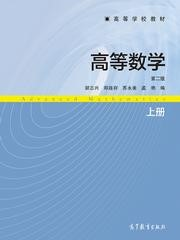
\includegraphics[width=\textwidth]{App1_1}
      \caption{上册.}
    \end{subfigure}
    \begin{subfigure}[b]{.23\textwidth}
      \centering
      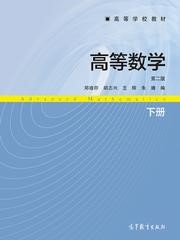
\includegraphics[width=\textwidth]{App1_2}
      \caption{下册.}
    \end{subfigure}
    \caption{北京科技大学 胡志兴等 编.高等数学(第二版),高等教育出版社.}\label{fig:教材}
  \end{figure}

  \hspace*{2em}再来说说如何入门。我们借一个例子来指出一些概念和知识上的错误,如\autoref{fig:一张错误的高等数学知识结构图}所示,
  \begin{figure}[!htb]
    \centering
    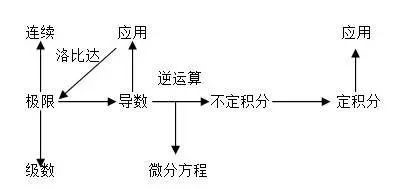
\includegraphics[width=.4\textwidth]{App1_3}
    \caption{一张错误的高等数学知识结构图.}\label{fig:一张错误的高等数学知识结构图}
  \end{figure}
  事实上,这张图不仅在内容上没有说清高等数学的梗概\footnote{应当包括一元函数微分学、一元函数积分学、向量代数与空间解析几何、多元函数微分学、多元函数积分学、无穷级数以及常微分方程七大板块,图中只提及了三个板块。}
  ,甚至在正确性上也令人怀疑。例如,极限是微积分的基础,用一个箭头从导数的应用指向极限,而这个箭头上标注着洛必达法则是合适的吗\footnote{作者的本意可能是指可以利用洛必达法则来计算函数的极限,但这仅仅是高等数学里一个非常细节性的知识点,把它放在概括高等数学全貌的知识结构图里是不合适的。}
  ?再如,导数与不定积分互为逆运算,为何没有用双向箭头连接?不是所有的定积分都可以通过不定积分计算(有的被积函数并不存在原函数,却是可积的),那么凭什么用一个箭头从不定积分指向定积分呢?这些问题尽管细节,却正说明这张图的作者并没有深入理解微积分这门学科里的概念,而只是浅尝辄止,至多停留于“考好即可”的地步。读者若想真正学好这门课,就绝不能有这样的想法——至少,课本上没有打星号指明可读可不读的章节,一定要反复读,学完之后还要回过头来思考各章节之间的联系。这样的学习甚至可能需要持续到本科高年级阶段。笔者在考研复习时整理的高等数学知识点结构图之某部分(未完成)如\autoref{fig:笔者在考研复习时整理的高等数学知识点结构图之某部分(未完成)}所示。
  \begin{figure}[!htb]
    \centering
    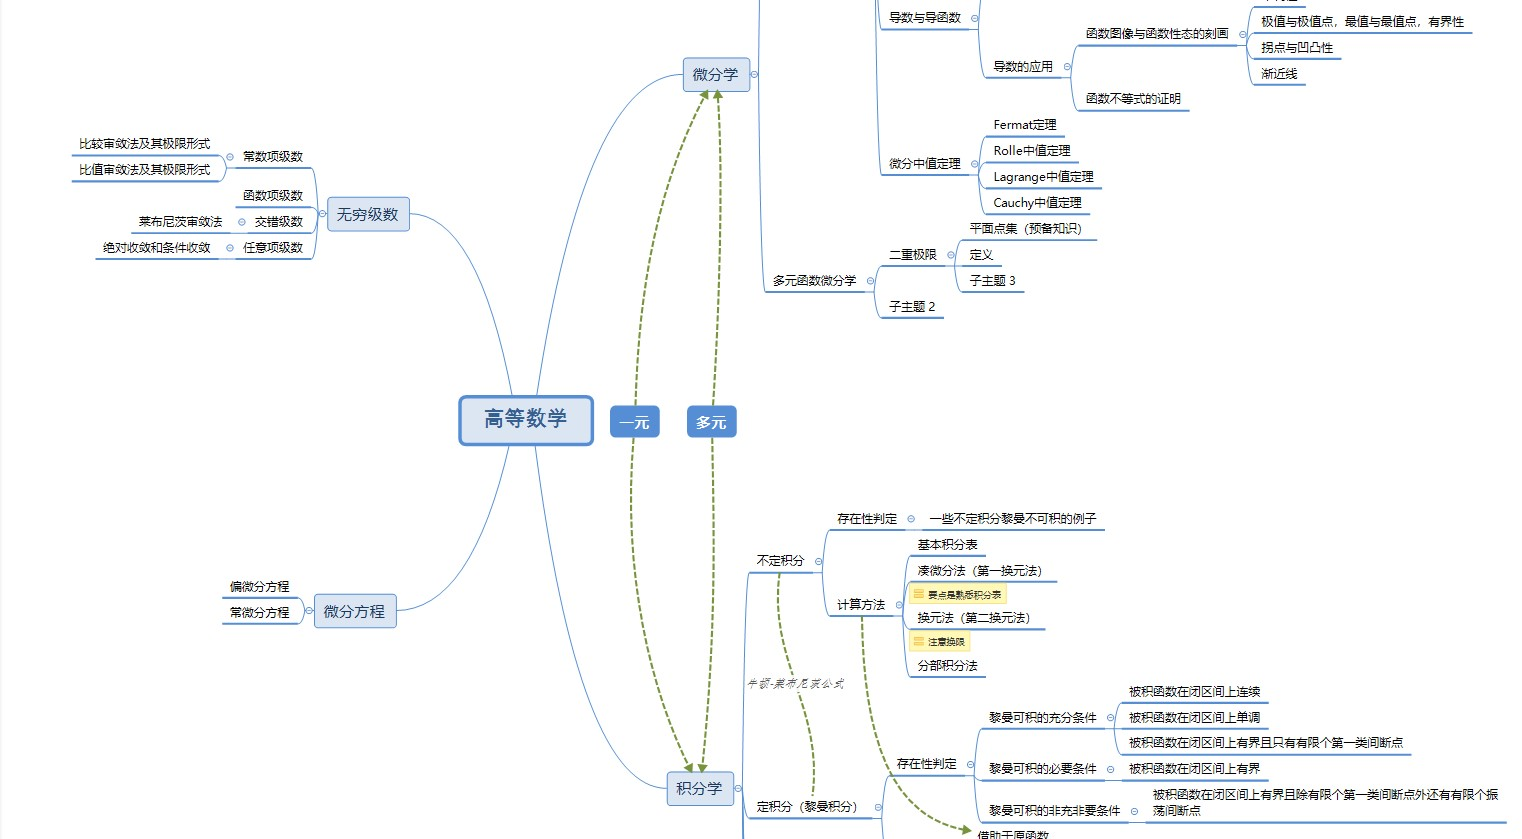
\includegraphics[width=.75\textwidth]{App1_4}
    \caption{笔者在考研复习时整理的高等数学知识点结构图之某部分(未完成).}\label{fig:笔者在考研复习时整理的高等数学知识点结构图之某部分(未完成)}
  \end{figure}

  \hspace*{2em}说完了这门学科大体上应当如何学习,我们再来聊点具体的、同时也是大家最关注的,那就是具体到课上课下时应该怎么做。笔者的经验是:高效的预习工作是每一轮学习中最重要的部分,课堂听讲抓住重点是必不可少的部分,课后及时的复习和总结是收获最大的部分。这样说是因为,高等数学这门课程抽象性比较强,概念多而且联系紧密、深刻而富有内涵,课程时间跨度大、强度大,课后练习题型丰富。尽管每年考试的题型大同小异,难度也很友好,但仍不能就此掉以轻心,而必须重视每一轮学习的每一个环节。

  \hspace*{2em}在课前预习部分,要做到了解下一堂课会提到哪些概念,这些概念同已经学过的部分有什么联系(例如,是从什么问题引出的,与之相关的命题是否能被前文所述的定理证明,等等);课堂上要重点关注两方面,一是老师是如何讲解自己在预习时尚未理解的部分,二是老师是如何解题的;课后复习要及时清完习题,以及再次阅读课本——对照老师在课堂上讲述的观点,以期加深理解、弥补不足。

  \hspace*{2em}在除教材以外的其他参考资料方面,学弟学妹们不必担心。自2009年自主编辑第一版《高等数学》、2013年修订编辑第二版《高等数学》,乃至学生讲师团建立以来,校内的各类资料可以说是无比丰富了。笔者自己使用过的纸质资料里,除物美复印店里可以找到的《高等数学练习册(2013版)》,以及期中、期末考试前讲师团发下的历年考试题外,还有其他一些学校的试卷,以及《吉米多维奇数学分析习题集学习指引》(谢惠民)、《高等数学复习指导——思路、方法与技巧》(陈文灯)、《大学生数学竞赛习题精讲》(陈兆斗)等等,至于电子版资料就更是数不胜数了,笔者使用过的部分电子版资料如\autoref{fig:笔者使用过的部分电子版资料}所示。
  \begin{figure}[!htb]
    \centering
    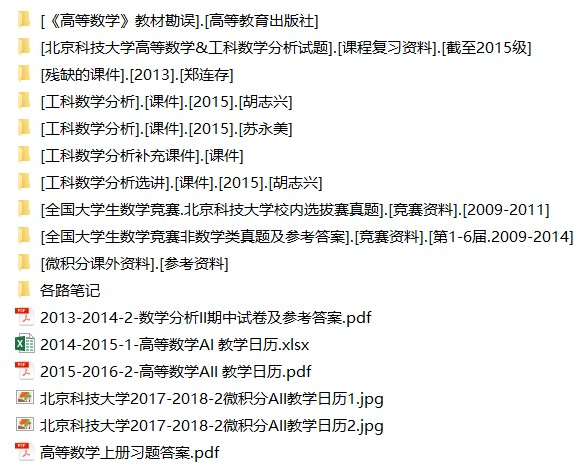
\includegraphics[width=.43\textwidth]{App1_5}
    \caption{笔者使用过的部分电子版资料.}\label{fig:笔者使用过的部分电子版资料}
  \end{figure}

  \hspace*{2em}总地来说,对于普通本科生而言,过于拔高习题的难度是没有太大意义的,但仅仅局限于课后习题也难以让学生深刻理解知识点(尽管我说的“深刻理解”可能不是读者以为的“深刻理解”)。斟酌再三,笔者认为在课后习题保质保量完成,而课余时间仍然充足的前提下,适当地看一些课外书、了解一些竞赛知识、做一些竞赛题是可以的,而刷大量的历年考试题则是没有必要的。个中滋味、如何平衡就待诸君正式开始学习之后,自行体会吧!

\section{学好高等数学有什么必要性以及帮助}
  \begin{marker}
  {\heiti 第三个问题:学习高等数学的意义在于什么?对于今后的学习、工作乃至生活有什么帮助?}
  \end{marker}

  \hspace*{2em}在谈论学习某一门学科的必要性之前,必须先了解这门学科的意义;而在了解其意义之后,“为什么要学习/不必学习这门课”也就不证自明了。

  \hspace*{2em}大而言之,冯·诺依曼在论述微积分时曾这样评价:“微积分是现代数学取得的最高成就,对它的重要性怎样估计也是不会过分的。”而今天,在微积分问世300余年之后,它依然值得被这样赞美——这不仅仅是因为其广泛而又重要的应用,更是由于人类在攀登这座高峰的历程中付出的艰辛努力,以及由此在思想史上写下的辉煌篇章。小而言之,今后几乎任何领域的研究工作的推进——从人工智能的训练模式到城市排水系统的改进,从航天器的设计到交通灯的安排……都要依靠、或者至少是借助数学工具,而微积分则是这些工具里最基础并且重要的之一。

  \hspace*{2em}以笔者自己学习专业课的经历为例,微积分工具乃至在大一大二其他课程里学习过的数学工具,在很多专业课里都有应用。例如,在经济学理论里经常要研究一些复杂的情况,这些情况通常被很多个因素影响。为了研究一种可变因素的数量变动会对其他可变因素的变动产生多大影响,需要用到边际分析方法,而“边际”这个概念回归到微积分理论里正是最基本的概念之一——导数。再如,理解计量经济学中的各种模型,需要先修微积分、线性代数、运筹学、概率论等多门基础数学课的知识,其中有一种GARCH模型,它应用于分析具有波动性集群效应的微观金融数据,或持有某项资产的风险(异方差)的情况。GARCH模型的基本形式GARCH$(p,q)$写为
  \begin{subnumcases}{}
    {y_t} = {{x'}_t}\phi  + {u_t}, \quad {u_t} \sim N\left( {0,\sigma _t^2} \right) \\
    \sigma _t^2 = {\alpha _0} + \sum_{i = 1}^p {{\alpha _i}u_{t - i}^2}  + \sum_{j = 1}^q {{\beta _j}\sigma _{t - j}^2} \label{equ:GARCH}
  \end{subnumcases}
  在平稳随机过程的条件下\autoref{equ:GARCH}也可以写成
  $\sigma _t^2 = \beta {\left( L \right)^{ - 1}}{\alpha _0} + \beta {\left( L \right)^{ - 1}}\alpha \left( L \right)u_t^2$
  的形式,而这两种形式之间的变换则要涉及到微分算子\footnote{读者将会在大一年级下学期的《高等数学\ROMAN{1}》或《工科数学分析\ROMAN{2}》课程里首次接触到“微分算子”的概念。}
  的概念了。定义这样一个平稳过程中的滞后算子:
  \[ \begin{cases}
    \alpha \left( L \right) = {\alpha _1}L + {\alpha _2}{L^2} +  \cdots  + {\alpha _p}{L^p} \hfill \\
    \beta \left( L \right) = 1 - {\beta _1}L - {\beta _2}{L^2} -  \cdots  - {\beta _p}{L^p}
  \end{cases} \]
  \hspace*{2em}于是有
  $\beta \left( L \right)\sigma _t^2 = {\alpha _0} + \alpha \left( L \right)u_t^2$
  ,代入\autoref{equ:GARCH}便得到其变换后的形式。

  再如,对于借助计算机研究各种工程现象的工程人员来讲,求解一个代数方程通常要比求解一个微分方程容易得多,而要将微分方程转化为代数方程则需要使用积分变换的方法。例如,经典控制理论中对控制系统的分析和综合都建立在Laplace变换的基础上,而引入拉普拉斯变换的一个主要优点,是可以用传递函数代替常系数微分方程来描述系统的特性,为采用直观和简便的图解方法来确定控制系统特性、分析控制系统的运动过程,以及控制系统的参数整定提供极大的便利。而要想理解Laplace变换,就必须先修微积分课程里的积分学,并深入理解复变函数的概念和性质。

  \hspace*{2em}当然,也有同学志不在科研或深造,而是希望毕业之后投身职业圈——怀有这样志向的学生并不少见,也并无可指摘之处,但若就此认为大学里的高等数学(乃至某些其他必修课程)是没有必要学习的,那笔者只好送他们一句流传甚广的玩笑话了:“数学不能用来买菜,却可以决定你在哪里买菜。”

\section{一些笔者推荐的课外数学资料}
~
  \subsection{书籍}
    \hspace*{2em}必须事先指出的是,以下这些书籍不一定对“使课程取得高分”有用,而仅以飨读者之思想。排名不分先后,尽可凭兴趣阅读。
  \begin{enumerate}[label=(\arabic*),leftmargin=4em]
    \item 《数学——它的内容、方法和意义》[俄]A.D.亚历山大洛夫 等 著

    本书由前苏联数位著名数学家为普及数学知识而合力撰写,介绍了现代数学各个分支的内容、历史发展及其在自然科学和工程技术中的应用,语言通俗简练,内容由浅入深,可供高等院校理工科师生、普通高中师生、工程技术人员和数学爱好者阅读。

    \item 《古今数学思想》[美]Morris Klein 著

    本书论述了从古代一直到20世纪头几十年中的重大数学创造和发展,目的是介绍中心思想,特别着重于那些在数学历史的主要时期中逐渐冒出来并成为最突出的、并且对于促进和形成尔后的数学活动有影响的主流工作。不同于一般数学史的著作,而主要作为“从历史角度来讲解的数学入门书”,该书突出了数学发展历程中涌现的各类思想方法,论述了数学思想的古往今来,被誉为“我们现有的数学史中最好的一本数学史”。

    \item 《微积分的历程:从牛顿到勒贝格》[美]William Dunham 著

    本书宛如一座陈列室,汇聚了十多位数学大师的杰作,当你徜徉其中时会对人类的想象力惊叹不已,当你离去时必然满怀对天才们的钦佩感激之情。作者同读者一起分享了分析学历史中为人景仰的理论成果。书中的每一个结果,从牛顿的正弦函数的推导,到伽玛函数的表示,再到贝尔的分类定理,无一不处于各个时代的研究前沿,至今还闪烁着耀眼夺目的光芒。
  \end{enumerate}
    \begin{figure}[!htb]
      % \centering
    \hfill
    \begin{subfigure}[b]{.2\textwidth}
      \centering
      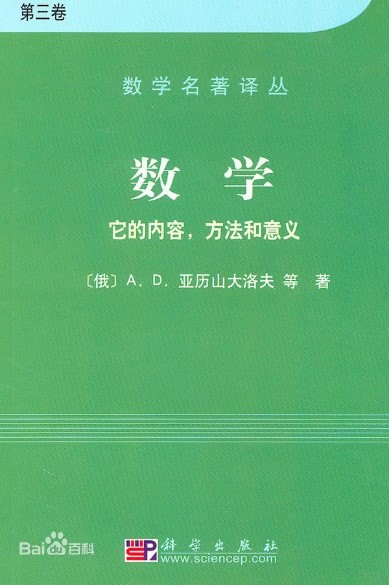
\includegraphics[width=\textwidth]{App1_6}
      \caption{《数学——它的内容、方法和意义》[俄]A.D.亚历山大洛夫 等 著.}
    \end{subfigure}
    \hfill
    \begin{subfigure}[b]{.2\textwidth}
      \centering
      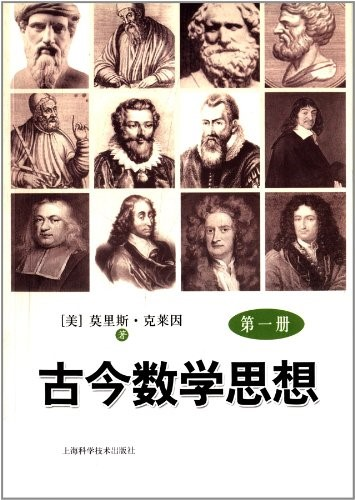
\includegraphics[width=\textwidth]{App1_7}
      \caption{《古今数学思想》[美]Morris Klein 著.}
    \end{subfigure}
    \hfill
    \begin{subfigure}[b]{.2\textwidth}
      \centering
      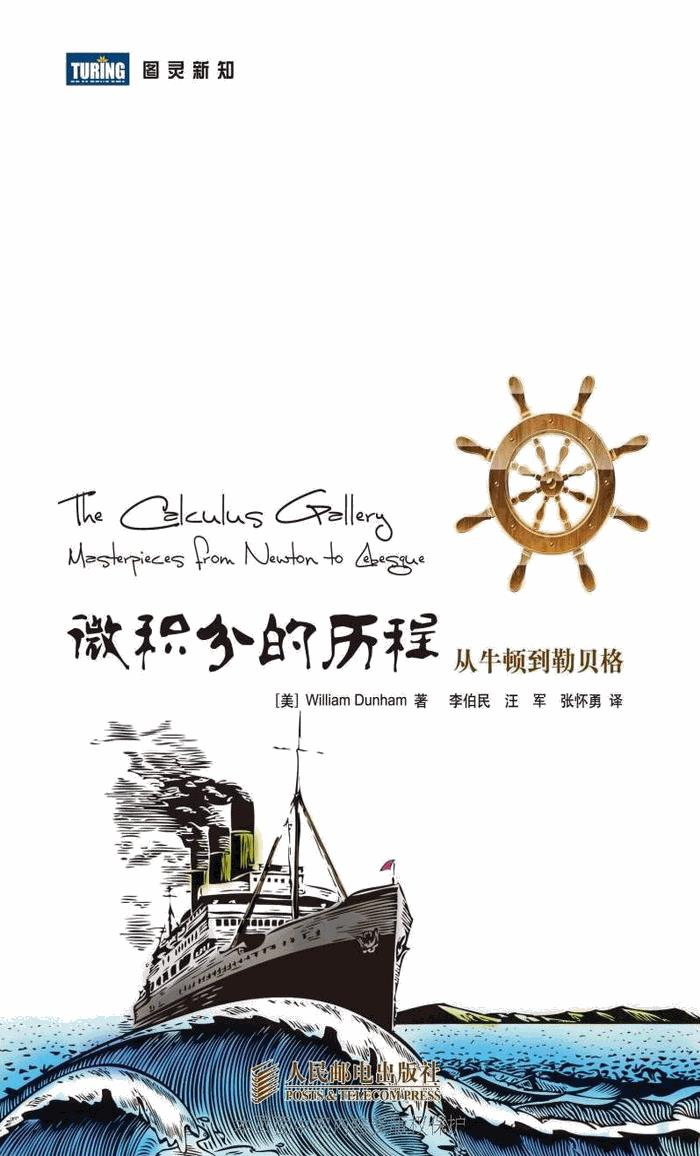
\includegraphics[width=\textwidth]{App1_8}
      \caption{《微积分的历程:从牛顿到勒贝格》[美]William Dunham 著.}
    \end{subfigure}
    \caption{笔者推荐的部分书目.}
  \end{figure}
  \hspace*{2em}当然,好书还有很多,为免贪多嚼不烂,笔者就不一一列举了。

  \subsection{公共资源平台}
    \hspace*{2em}除去本校学生讲师团为每届学弟学妹们建立的数学交流群之外,还有许多公共平台可以为希望提高自身数学水平(以在期末考试乃至数学竞赛中取得好成绩)的大学生提供各类学习资源,包括书籍、习题、文章等等。例如\autoref{fig:笔者推荐的部分微信公众号}所示微信公众号。
    \begin{figure}[!htb]
    \centering
    \hfill
    \begin{subfigure}[b]{.2\textwidth}
      \centering
      
\includegraphics[width=\textwidth]{App1_9}
      \caption{高等数学.}
    \end{subfigure}
    \hfill
    \begin{subfigure}[b]{.2\textwidth}
      \centering
      
\includegraphics[width=\textwidth]{App1_10}
      \caption{向老师讲数学.}
    \end{subfigure}
    \hfill
    \begin{subfigure}[b]{.2\textwidth}
      \centering
      
\includegraphics[width=\textwidth]{App1_11}
      \caption{考研竞赛数学.}
    \end{subfigure}
    \hfill
    \begin{subfigure}[b]{.2\textwidth}
      \centering
      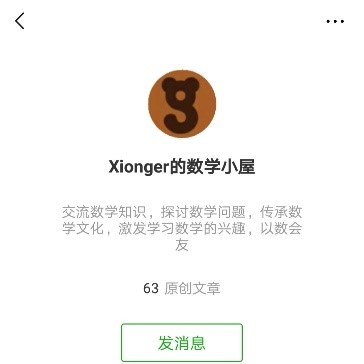
\includegraphics[width=\textwidth]{App1_12}
      \caption{Xionger的数学小屋.}
    \end{subfigure}
    \caption{笔者推荐的部分微信公众号.}\label{fig:笔者推荐的部分微信公众号}
    \end{figure}

    \hspace*{2em}有兴趣的学弟学妹们也可以自行搜索各种数学交流群(我的经验告诉我,大佬们都在各个QQ群里交流,就看你有没有本事加进去了),这里就不赘述了。


  \chapter{谈单变量微积分里几个基本的概念}
    % !TEX root = ./HTNotes-Demo.tex
% !TEX program = xelatex
\begin{flushright}
文/似雪飞扬
\end{flushright}

\section{预备知识}
  \subsection*{初等函数与分段函数}
    \begin{defn}
      由基本初等函数经过有限次四则运算和复合运算得到的,可以只用一个式子表达的函数称为初等函数.
    \end{defn}
    \begin{defn}
      由多个定义在不同区间上的式子组合在一次表达的函数称为分段函数.
    \end{defn}
    几点说明:
    \begin{enumerate}[label=(\arabic*)]
      \item 分段函数不一定不是初等函数.

      举例:$f(x) = \abs{x} =
      \begin{cases}
        x, & x \ge 0 \\
        -x, & x < 0
      \end{cases}
      = \sqrt{x^2}, x \in \mathbb{R}$.

      一般地,若分段函数$f(x)$的各段定义区间是连着的,且 是连续函数,则$f(x)$是初等函数.
      \item 基本初等函数在定义域上处处连续.
      \item 初等函数在各段定义区间上分别处处连续(在分段点处可能间断也可能连续).

      举例:$f(x) =\sin \dfrac{1}{x}, x \in \mathbb{R}$在$(0,+\infty)$, $(-\infty,0)$上均连续,而在原点处振荡间断.

      这个命题不放在微分学部分是因为一般将其作为不证自明的基本命题.
    \end{enumerate}

\section{一元函数微分学部分}
~ \subsection{连续、间断与可导}
    \hspace*{2em}讨论点态连续的前提是函数在该点邻域内有定义,讨论点态间断的前提是函数在该点去心邻域内有定义. 例如,对$f\left( x \right) =x$, $x\in \mathbb{Q}$讨论连续性是无意义的.

    \hspace*{2em}间断点的分类标准是两侧极限是否存在. 若函数在某点处间断但两侧极限均存在,则将该点定义为第一类间断点,并按两侧极限是否相等分为可去间断点和跳跃间断点(立即可知对于可去间断点必定有函数在该点处无定义的结论);若函数在某点两侧的极限至少有一侧不存在(或者两侧都不存在. 显然第二类间断点对该点是否有定义并无要求,可以有也可以没有),则将该点定义为第二类间断点,并按单侧极限不存在的方式是趋于无穷还是振荡将该侧间断分为无穷间断和振荡间断.

    \hspace*{2em}举例:
    $$f\left( x \right) =
    \begin{cases}
      \sin \dfrac{1}{x}, & x \ne 0\\
      0, & x=0 \\
    \end{cases}$$
    在原点处振荡间断,图像如\autoref{fig:一个常见振荡间断点的例子.}所示. 这也是也是振荡间断点最常用的例子.
    \begin{figure}[!h]
      \centering
      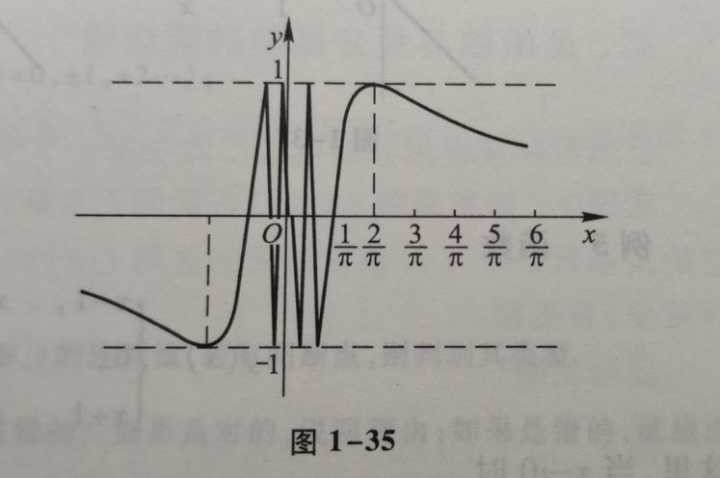
\includegraphics[width=.3\textwidth]{App2_1}
      \caption{一个常见振荡间断点的例子.}\label{fig:一个常见振荡间断点的例子.}
    \end{figure}

    几点说明:
    \begin{enumerate}[label={(\arabic*)}]
      \item  非初等函数可能只在某些点处连续,也可能处处不连续,但不可能几乎处处
      \footnote{“几乎处处”是数学分析中的一个说法. 若某性质P对于集合 中的每一个元素都成立,称性质P在集合 上处处成立;若性质P对于集合 中的每一个元素都成立,其中 是零测集,则称性质P在集合 上几乎处处成立. 这个概念我们还将会在积分学部分再次遇到.}
       连续.

      举例:狄利克雷(Dirichlet)函数
      \[ D\left( x \right) =\begin{cases}
        \text{1,}&    x\in \mathbb{Q}\\
        0, &    x\in \mathbb{R}\backslash\mathbb{Q}\\
      \end{cases} \]
      处处不连续,略作变化即可得到只在原点处连续的函数
      $$f\left( x \right) =x\rd \left( x \right) =\begin{cases}
        x,&   x\in \mathbb{Q}\\
        0, &    x\in \mathbb{R}\backslash\mathbb{Q}\\
      \end{cases}$$

      事实上,初等函数才是在其定义域上几乎处处连续的
      \footnote{举例:$\tan x$和$\tan \frac{1}{x}$在$\mathbb{R}$上几乎处处连续.}
      .

      \item 处处连续的函数在某点处不一定可导,甚至可能处处不可导.

      举例:$f\left( x \right) =
      \begin{cases}
        x\sin \dfrac{1}{x}, & x \ne 0\\
        0, & x=0 \\
      \end{cases}$
      处处连续但在原点处不可导;
      魏尔斯特拉斯(Weierstrass)函数
      $$f\left( x \right) =\sum_{i=1}^{\infty}{a^n\cos \left( b^n\pi x \right)}\left( a\in \left( 0, 1 \right) ,b=2k+\text{1,}k\in \mathbb{N},ab>1+\frac{3}{2}\pi \right) $$
      \begin{figure}[!h]
        \centering
        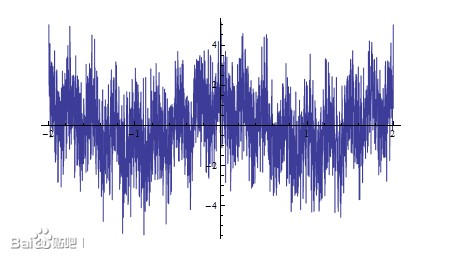
\includegraphics[width=.3\textwidth]{App2_2}
        \caption{Weierstrass函数图像示意图.}\label{fig:Weierstrass函数图像示意图.}
      \end{figure}
      处处连续但无处可导,如\ref{fig:Weierstrass函数图像示意图.}所示;

      \item 处处可导的函数,它的导函数在其定义域上不一定连续.

      举例:$f\left( x \right) =
      \begin{cases}
        x^2 \sin \dfrac{1}{x}, & x \ne 0\\
        0, & x=0 \\
      \end{cases}$.

      \item 函数在某点处的左右导数均存在(但不一定相等),则可以推出函数在该点连续.

      简单证明如下:由左右导数存在可知$\Delta y=\begin{cases}
        y'_-\left( x_0 \right) \cdot \Delta x,&   \Delta x<0\\
        y'_+\left( x_0 \right) \cdot \Delta x,&   \Delta x>0\\
      \end{cases}\rightarrow 0\left( \Delta x\rightarrow 0 \right)$.

      \item 函数在某点处可导,不一定在该点去心邻域内连续.

      举例:借助狄利克雷函数构造$f\left( x \right) =x^2\text{D}\left( x \right)$在$x=0$处可导,但在$\mathbb{R}\backslash\{0\}$内处处不连续.

      \item 导函数在某点处的极限存在,不能推知函数在该点连续.

      举例:$f\left( x \right) =\left[ \sgn \left( x \right) \right] ^2=\begin{cases}  \text{1,}&    x\ne 0\\  0, &    x=0\\\end{cases}$.

      \item 导函数在某点处的极限存在,且函数在该点处连续,则函数在该点可导,且导函数在该点连续.

      这个命题称为导数极限定理,可以通过洛必达法则证明:设$f(x)$在$x = x_0$处连续,且$\lim\limits_{x \to x_0} f'(x)$存在,则
      \[ f'\left( x_0 \right) =\underset{x\rightarrow x_0}{\lim}\frac{f\left( x \right) -f\left( x_0 \right)}{x-x_0}\xlongequal{\text{L'Hospital}}\underset{x\rightarrow x_0}{\lim}\frac{f'\left( x \right)}{1}=\underset{x\rightarrow x_0}{\lim}f'\left( x \right) \]

      \item 连续性是介值性
      \footnote{介值定理:定义在区间上的连续函数,其值域必定也是区间(可缩为一点). 该定理可借助零点存在定理,由构造函数法证明. 介值性:设$I_f=\left[ a,b \right], $若$\forall a\le x_1<x_2\le b,f\left( x_1 \right) \ne f\left( x_2 \right)$, $f\left( x \right) $可取到$f\left( x_1 \right) \text{和}f\left( x_2 \right) $之间的任意值,称$f$在$[a,b]$上具有介值性.}
      的充分不必要条件.

      举例:已在前文出现过的$f\left( x \right) =x\text{D}\left( x \right) =\begin{cases}
        x,&   x\in \mathbb{Q}\\
        0, &    x\in \mathbb{R}\backslash\mathbb{Q}\\
      \end{cases}$还告诉我们,区间上的函数即使处处不连续,也可以具有介值性.

      另外一个非常有意思的例子是导数介值定理(也被称为达布中值定理):闭区间上可导的函数,其导函数可以取到该区间两端点处导数值之间的一切值,即导函数具有介值性. 可以通过费马引理证明之,此处不再赘述.
    \end{enumerate}

  \subsection{可导、极值与单调性}
    \begin{enumerate}[label=(\arabic*)]

      \item 连续函数在某点处取得极值,不能推知函数在该点邻域内的单调性.
      举例:魏尔斯特拉斯函数在原点处取得极大值,但在原点的任意单侧去心邻域内不单调.

      \item 连续函数在某点可导且导数不为0,不能推知函数在该点邻域内的单调性.

      如2004年考研数学一8题/数学二10题:设函数$f(x)$连续,且$f'(0)>0$,则存在$\delta>0$,使得(\qquad)
      \options{在$(0,\delta)$内单调增加}
      {在$(-\delta,0)$内单调减少}
      {对任意的$x \in (0,\delta)$有$f(x)>f(0)$}
      {对任意的$x \in (-\delta,0)$有$f(x)>f(0)$}
      答案:C. 对错解AB构造反例:$f\left( x \right) =\begin{cases}
        x^2\sin \dfrac{1}{x} + \dfrac{x}{2}, & x\ne 0, \\
        0, & x=0 \\
      \end{cases}$.

      \item 可导函数在某点处导数为0是其在该点处取得极值的必要不充分条件.

      该命题可以通过费马引理证明,此处不加赘述.

      \item 函数在某点处连续、在该点去心邻域内可导且导函数在该点两侧变号,是其在该点处取得极值的第一充分不必要条件.

      这一点也警示我们,讨论极值点时不能仅看函数的导数为0的点,还应当关注其不可导的点. 例如对于函数$f(x) = \sqrt{\abs{x}}, x \in \mathbb{R}$,其在原点处不可导,但在原点处取得极小值,如\ref{fig:原点不可导但是在原点取得极限值的一个例子.}所示.
      \begin{figure}[!h]
        \centering
        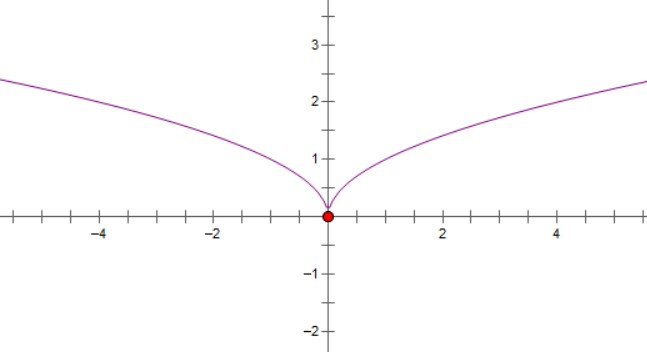
\includegraphics[width=.3\textwidth]{App2_3}
        \caption{原点不可导但是在原点取得极限值的一个例子.}\label{fig:原点不可导但是在原点取得极限值的一个例子.}
      \end{figure}

      \item 函数在某点处二阶可导且在该点处一阶导数为0、二阶导数不为0,是其在该点处取得极值的第二充分不必要条件. 该条件还可推广为在某点处偶数阶可导且除最高阶导数值外其他阶导数均为0.
    \end{enumerate}

  \subsection{二阶可导与凹凸性}
    \hspace*{2em}连续函数在某点处存在二阶导数,且该点处一阶导等于0、二阶导不等于0,不能推知函数在该点邻域内的凹凸性.

    如这样一题:设函数$f(x)$在$x = x_0$处存在二阶导数,且$f'(x_0)=0$, $f''(x_0)<0$,则必定存在$\delta > 0$使得(\qquad)
    \options{曲线$y=f(x)$在区间$(x_0 - \delta, x_0 + \delta)$上是凸的}
    {曲线$y=f(x)$在区间$(x_0 - \delta, x_0 + \delta)$上是凹的}
    {函数$f(x)$在区间$(x_0-\delta,x_0]$上严格单增,在区间$[x_0, x_0+\delta)$上严格单减}
    {函数$f(x)$在区间$(x_0-\delta,x_0]$上严格单减,在区间$[x_0, x_0+\delta)$上严格单增}
    答案:C. 对错解AB构造反例:$f\left( x \right) = \displaystyle\int_0^x{\left( t^2\sin \frac{1}{t}+\frac{t}{2} \right) \rd t}$.

  \subsection{后记}
    \hspace*{2em}以上举出的函数,有能力的话最好自己尝试作出图像或草图,以加深理解.
    最后留一道习题:讨论函数
    $f\left( x \right) =\begin{cases}
      ax^{\lambda}+bx^{\alpha}\sin \left( x^{\beta} \right), & x\ne 0 \\
      0, & x=0 \\
    \end{cases}\left( a,b,\alpha ,\beta ,\lambda \in \mathbb{R} \right)$
    在原点处存在几阶导数,各阶导函数在原点处是否连续.

\section{一元函数积分学部分}
~ \subsection{定积分与不定积分,可积与原函数,以及变限积分}
    \begin{enumerate}[label=(\arabic*)]
      \item 定积分存在$\Leftrightarrow$可积,不定积分存在$\Leftrightarrow$原函数存在.
      \item 不定积分和定积分是两个概念,不定积分存在不一定可积,可积也不一定有原函数.
      \item 变限积分借助微积分基本定理和Newton-Leibniz公式担当了沟通定积分和不定积分的桥梁,但要注意对被积函数的可积性/连续性、变限积分的连续性/可导性的区分.
    \end{enumerate}

  \subsection{可积(定积分存在)的三类条件}
    \begin{enumerate}[label=(\arabic*)]
      \item 必要不充分条件:有限区间上有界

      若不满足有限区间,立即成为无穷限的反常积分;若不满足有界,立即成为无界的反常积分. 对不满足充分性举例:狄利克雷函数在闭区间$[0,1]$上有界,但不可积.
      \item 充分不必要条件:
      \begin{enumerate}[label=(\roman*)]
        \item 闭区间上连续.

        注意和上文必要不充分条件里的“有限区间”区分开,前者可以是开区间(采用补充定义法立即变为闭区间),而这里必须是闭区间(开区间上的连续函数可能无界).
        \item 闭区间上有界,且只有有限个间断点.

        注意:第一,这里的间断点不能是无穷间断点;第二,教材上一般写为“且只有有限个第一类间断点”,并未讨论振荡间断点的情况. 实际上闭区间内含有有限个振荡间断点的有界函数也是可积的(但不一定有原函数),如
        $f\left( x \right) =\begin{cases}
          2x\sin \dfrac{1}{x}-\cos \dfrac{1}{x},&   x\ne 0\\
          0, &    x=0\\
        \end{cases}$
        在$[0,1]$上的定积分为$\sin 1$.
        对不满足必要性举例:函数$\sgn\left(\sin\dfrac{x}{\pi}\right)$在$[0,1]$上有无穷个间断点(一个振荡间断点$x = 0$以及可列无穷个跳跃间断点$x_k = \frac{1}{k}, k \in \mathbb{N}^\ast$),但可积. 具体为何可积将在充要条件里介绍.
        \item 闭区间上单调.
      \end{enumerate}
      \item 充要条件(注意,这部分超纲!)
      若定义在闭区间$[a,b]$上且有界的函数$f(x)$的全体间断点构成的集合是零测度集,则$f(x)$在$[a,b]$上(勒贝格)可积,逆命题也成立.

        注:把可以用总长度任意小的有限个区间覆盖的点集称为“零测度集”,简称零集. 上文中跳跃间断点$x_k = \frac{1}{k}, k \in \mathbb{N}^\ast$构成的集合是可数无穷集,故而为零测集.

      上述充要条件也表述为:区间上的有界函数可积的充要条件是几乎处处连续.
    \end{enumerate}

  \subsection{原函数(不定积分)存在的条件}
    \begin{enumerate}[label=(\arabic*)]
      \item 必要不充分条件:$f(x)$有原函数,则必定不含有第一类间断点或无穷间断点.
      \item 充分不必要条件:$f(x)$连续,则必定有原函数.
      \item 既非充分也非必要,需分类讨论:$f(x)$含有振荡间断点,则原函数不一定不存在.

      举例:$f\left( x \right) =\begin{cases}
        2x\sin \dfrac{1}{x}-\cos \dfrac{1}{x},&   x\ne 0\\
        0, &    x=0\\
      \end{cases}$
      有原函数
      $F\left( x \right) =\begin{cases}
        x^2\sin \dfrac{1}{x},&   x\ne 0\\
        0, &    x=0\\
      \end{cases}$.
    \end{enumerate}

\section{参考文献}
\begin{enumerate}[label={[\arabic*]}]
  \item 张宇等.~2019张宇高等数学18讲[M].北京:高等教育出版社,2017.12:120.
  \item 同济大学数学系.高等数学.第7版[M].北京:高等教育出版社,2017,9:59.
  \item 胡志兴等.高等数学.第2版[M].北京:高等教育出版社,2015.6:161.
  \item 谢惠民等.吉米多维奇数学分析习题集学习指引(第二册)[M].北京:高等教育出版社,2012,12:121-122.
  \item 谢惠民.数学分析习题课讲义上册[M].北京:高等教育出版社,2003:132
\end{enumerate}

  \chapter{高等数学常用公式表}
    % !TEX root = ./HTNotes-Demo.tex
\section{基本初等函数导数、微分公式}
  \begin{center}
    \begin{tabular}{r @{\qquad} c @{\qquad} l}
    \toprule[1pt]
      原函数 & 导数 & 微分\\
    \midrule[0.5pt]
      $y=\mathrm{C}$ & $y' = 0$ & $\rd y = 0$\\
      $y=x^\mu$ & $y' = \mu x^{\mu - 1}$ & $\rd y = \mu x^{\mu - 1} \rd x$\\
      $y = \sin x$ & $y' = \cos x \rd x$ & $\rd y = \cos x \rd x$\\
      $y = \cos x$ & $y' = - \sin x \rd x$ & $\rd y = - \sin x \rd x$\\
      $y = \tan x$ & $y' = \sec ^2 x$ & $\rd y = \sec ^2 x \rd x$\\
      $y = \cot x$ & $y' = - \csc ^2 x \rd x$ & $\rd y = - \csc ^2 x \rd x$\\
      $y = \sec x$ & $y' = \sec x \tan x$ & $\rd y = \sec x \tan x \rd x$\\
      $y = \csc x$ & $y' = -\csc x \cot x$ & $\rd y = -\csc x \cot x \rd x$\\
      $y = a^x$ & $y' = a^x \ln a$ & $\rd y = a^x \ln a \rd x$\\
      $y = e^x$ & $y' = e^x$ & $\rd y = e^x \rd x$\\
      $y = \log_a x$ & $y' = \frac{1}{x \ln a}$ & $\rd y = \frac{1}{x \ln a} \rd x$\\
      $y = \ln x$ & $y' = \frac{1}{x}$ & $\rd y = \frac{1}{x} \rd x$\\
      $y = \arcsin x$ & $y' = \frac{1}{\sqrt{1-x^2}}$ & $\rd y = \frac{1}{\sqrt{1-x^2}} \rd x$\\
      $y = \arccos x$ & $y' = - \frac{1}{\sqrt{1-x^2}}$ & $\rd y = - \frac{1}{\sqrt{1-x^2}} \rd x$\\
      $y = \arctan x$ & $y' = \frac{1}{1+x^2}$ & $\rd y = \frac{1}{1+x^2} \rd x$\\
      $y = \mathrm{arccot\,} x$ & $y' = - \frac{1}{1+x^2}$ & $\rd y = - \frac{1}{1+x^2} \rd x$\\
      $y = \mathrm{sh\,}x$ & $y' = \mathrm{ch\,} x$ & $\rd y = \mathrm{ch\,} x \rd x$\\
      $y = \mathrm{ch\,}x$ & $y' = \mathrm{sh\,} x$ & $\rd y = \mathrm{sh\,} x \rd x$\\
      $y = \mathrm{th\,} x$ & $y' = \frac{1}{\mathrm{ch}^2 \,x}$ & $\rd y = \frac{1}{\mathrm{ch}^2 \,x} \rd x $\\
    \bottomrule[1pt]
    \end{tabular}
  \end{center}

\newpage
\section{基本导数、微分法则}
  \begin{tabular}{r @{\qquad} c @{\qquad} l}
  \toprule[1pt]
    函数 & 导数法则 & 微分法则\\
  \midrule[0.5pt]
    $u(x) \pm v(x)$ & $\left[ u(x) \pm v(x) \right]' = u'(x) \pm v'(x)$ & $\rd (u \pm v) = \rd u \pm \rd v$\\
    $u(x)v(x)$ & $\left[ u(x)v(x) \right]' = u'(x)v(x) + u(x)v(x)'$ & $\rd (uv) = v \rd u + u \rd v$\\
    $\mathrm{C}u$ & $(\mathrm{C}u)' = \mathrm{C}u'$ & $\rd (\mathrm{C}u) = C\rd u$\\
    $\frac{u(x)}{v(x)}$ & $\left( \frac{u(x)}{v(x)} \right)' = \frac{u'(x)v(x) - u(x)v(x)'}{v^2(x)}$ & $\rd \left( \frac{u}{v} \right) = \frac{v \rd u - u \rd v}{v^2(x)}$\\
    $\frac{1}{v(x)}$ & $\left( \frac{1}{v(x)} \right)' = - \frac{v'(x)}{v^2(x)}$ & $\rd \left( \frac{1}{v} \right) = - \frac{\rd v}{v^2}$\\
    $x=f(y)$ & $\left[ f^{-1}(y) \right]' = \frac{1}{f'(y)}$ & $\frac{\rd y}{\rd x} = \frac{1}{\frac{\rd x}{\rd y}}$\\
  \bottomrule[1pt]
  \end{tabular}

\section{常见高阶导数}
  \begin{tabular}{r @{\qquad} l @{\qquad} r @{\qquad} l}
  \toprule[1pt]
    函数 & 高阶导数 & 函数 & 高阶导数 \\
  \midrule[0.5pt]
    $e^x$ & $e^x$ & $\ln (1-x)$ & $- \frac{(n-1)\mathrm{!}}{(1-x)^n}$\\
    $\sin x$ & $\sin (x + n \cdot \frac{\pi}{2})$ & $\frac{1}{x}$ & $(-1)^n \cdot \frac{n\mathrm{!}}{x^(n+1)}$\\
    $\cos x$ & $\cos (x + n \cdot \frac{\pi}{2})$ & $\frac{1}{(1+x)}$ & $(-1)^n \cdot \frac{n\mathrm{!}}{(1+x)^(n+1)}$\\
    $x^\alpha$ & $\alpha(\alpha-1)\cdots(\alpha-n+1)x^{\alpha-n}$ & $\frac{1}{(1-x)}$ & $- \frac{n\mathrm{!}}{(1-x)^(n+1)}$\\
    $\ln (1+x)$ & $(-1)^n \cdot \frac{(n-1)\mathrm{!}}{(1+x)^n}$\\
  \bottomrule[1pt]
  \end{tabular}

\section{微分中值定理}
  \begin{description}
    \item[Fermat~引理] 设函数~$f(x)$~在点~$x_0$~的某领域~$U(x_0)$~内有定义,并且在~$x_0$~处可导,如果对任意的~$x \in U(x_0)$,有~$f(x) \le f(x_0)$~(或~$f(x) \ge f(x_0)$~),那么~$f'(x_0)=0$.
    \item[Rolle~定理] 如果函数~$f(x)$~满足:\ding{192}~在闭区间~$[a, b]$~连续,\ding{193}~在开区间~$(a, b)$~可导,\ding{194}~$f(a)=f(b)$,那么在~$(a, b)$~内至少有一点~$\xi(a<\xi<b)$~使得~$f'(\xi)=0$.
    \item[Lagrange~中值定理] 如果函数~$f(x)$~满足:\ding{192}~在闭区间~$[a, b]$~连续,\ding{193}~在开区间~$(a, b)$~可导,那么在~$(a, b)$~内至少有一点~$\xi(a<\xi<b)$~使等式~$f'(\xi)=\frac{f(b)-f(a)}{b-a}$~成立.
    \item[Cauchy~中值定理] 如果函数~$f(x)$~及~$F(x)$~满足:\ding{192}~在闭区间~$[a, b]$~连续,\ding{193}~在开区间~$(a, b)$~可导,\ding{194}对~$\forall x \in (a, b)$,$F(x)\ne0$,那么在~$(a, b)$~内至少有一点~$\xi(a<\xi<b)$~使等式~$\frac{f'(\xi)}{F(\xi)}=\frac{f(b)-f(a)}{F(b)-F(a)}$~成立.
  \end{description}

\section{Taylor~公式}
  \begin{enumerate}[label=\arabic*., leftmargin=2em ]
  \item Taylor~公式
    \begin{enumerate}[label=(\arabic*)]
      \item Lagrange~型余项
      $$f(x)=f(0)+f'(x_0)(x-x_0)+\dfrac{f''(x_0)}{2\text{!}}(x-x_0)^2+\cdots+\dfrac{f^{(n)}(x_0)}{n\text{!}}(x-x_0)^n+R_n$$
      其中,$R_n=\dfrac{f^{(n+1)}(\xi)}{(n+1)\text{!}}(x-x_0)^{(n+1)}$.
      \item Peano~型余项
      $$f(x)=f(x_0)+f'(x_0)(x-x_0)+\dfrac{f''(x_0)}{2\text{!}}(x-x_0)^2+\cdots+\dfrac{f^{(n)}(x_0)}{n\text{!}}(x-x_0)^n+o(x^n)$$
      \item 积分型余项
      $$f(x)=f(x_0)+f'(x_0)(x-x_0)+\dfrac{f''(x_0)}{2\text{!}}(x-x_0)^2+\cdots+\dfrac{f^{(n)}(x_0)}{n\text{!}}(x-x_0)^n+R_n$$
      其中,$R_n=\dfrac{1}{n\text{!}} \int_{x_0}^x (x-t)^n f^{(n+1)}(t)\rd t$.
    \end{enumerate}
  \item Maclaurin~公式(Peano~型余项)
    $$f(x)=f(0)+f'(0)x+\dfrac{f''(0)}{2\text{!}}x^2+\cdots+\dfrac{f^{(n)}(0)}{n\text{!}}x^n+o(x^n)$$
  \item 常用~Maclaurin~公式(Peano~型余项)
    \begin{enumerate}[label=(\arabic*)]
      \item $e^x = 1+x+\dfrac{1}{2\text{!}}x^2+\cdots+\dfrac{1}{n\text{!}}x^n+o(x^n)$
      \item $\sin x = x-\dfrac{1}{3\text{!}}x^3+\dfrac{1}{5\text{!}}x^5+\cdots+\dfrac{(-1)^n x^(2n-1)}{(2n-1)\text{!}}x^n+o(x^{2n})$
      \item $\cos x = 1-\dfrac{1}{2\text{!}}x^2+\dfrac{1}{4\text{!}}x^4+\cdots+\dfrac{(-1)^n x^2n}{(2n)\text{!}}x^n+o(x^{2n})$
      \item $\ln (1+x) = 1-\dfrac{1}{2}x^2+\dfrac{1}{3}x^3+\cdots+\dfrac{(-1)^(n+1) x^n}{n}x^n+o(x^{(n+1)})$
      \item $(1+x)^\alpha = 1+\alpha x+\cdots+\dfrac{\alpha(\alpha-1)\cdots(\alpha-n+1)x^{\alpha-n}}{n\text{!}}x^n+o(x^n)$
      \item $\arctan x = -x+\dfrac{1}{3}x^3-\dfrac{1}{5}x^5+\cdots+\dfrac{(-1)^n x^(2n+1)}{(2n+1)}x^n+o(x^{2n+2})$
      \item $\tan x = x+\dfrac{1}{3}x^3+\dfrac{2}{5}x^5+\dfrac{17}{315}x^7+o(x^7)$
    \end{enumerate}
  \end{enumerate}

\section{基本积分表}
\begin{tabenum}[(1)]
  \tabenumitem $\displaystyle\int k \rd x = kx + \text{C}$ ;\quad
  \tabenumitem $\displaystyle\int x^\alpha \rd x = \dfrac{1}{\alpha+1} x^{\alpha+1} + \text{C}\ (\alpha \ne -1)$;\\
  \tabenumitem $\displaystyle\int \dfrac{1}{x} \rd x = \ln x + \text{C}$;
  \tabenumitem $\displaystyle\int \dfrac{1}{1+x^2} \rd x = \tan x + \text{C}$;\\
  \tabenumitem $\displaystyle\int \dfrac{1}{\sqrt{1-x^2}} \rd x = \arcsin x + \text{C}$;
  \tabenumitem $\displaystyle\int \cos x \rd x = \sin x + \text{C}$;\\
  \tabenumitem $\displaystyle\int \sin x \rd x = - \cos x + \text{C}$;
  \tabenumitem $\displaystyle\int \sec^2 x \rd x = \tan x + \text{C}$;\\
  \tabenumitem $\displaystyle\int \csc^2 x \rd x = - \cot x + \text{C}$;
  \tabenumitem $\displaystyle\int e^x x \rd x = e^x + \text{C}$;\\
  \tabenumitem $\displaystyle\int a^x \rd x = \dfrac{a^x}{\ln a} + \text{C}$;
  \tabenumitem $\displaystyle\int \text{sh\,} x \rd x = \text{ch\,} x + \text{C}$;\\
  \tabenumitem $\displaystyle\int \text{ch\,} x \rd x = \text{sh\,} x + \text{C}$;
  \tabenumitem $\displaystyle\int \tan x \rd x = \ln \left| \cos x \right| + \text{C}$;\\
  \tabenumitem $\displaystyle\int \cot x \rd x = \ln \left| \sin x \right| + \text{C}$;
  \tabenumitem $\displaystyle\int \sec x \rd x = x \ln \left|\sec x + \tan x \right| + \text{C}$;\\
  \tabenumitem $\displaystyle\int \csc x \rd x = x \ln \left|\csc x + \cot x \right| + \text{C}$;
  \tabenumitem $\displaystyle\int \dfrac{1}{x^2 + a^2} \rd x = \dfrac{1}{a} \tan \dfrac{x}{a} + \text{C}$;\\
  \tabenumitem $\displaystyle\int \dfrac{1}{x^2 - a^2} \rd x = \dfrac{1}{2a} \ln \dfrac{x-a}{x+a} + \text{C}$;
  \tabenumitem $\displaystyle\int \dfrac{1}{\sqrt{x^2 - a^2}} \rd x = \arcsin \dfrac{x}{a} + \text{C}$;\\
  \tabenumitem $\displaystyle\int \dfrac{1}{\sqrt{x^2 \pm a^2}} \rd x = \ln \left|x + \sqrt{x^2 \pm a^2} \right| + \text{C}$;
  \tabenumitem $\displaystyle\int \sec x \tan x \rd x = \sec x + \text{C}$;\\
  \tabenumitem $\displaystyle\int \csc x \cot x \rd x = - \csc x + \text{C}$;
  \tabenumitem $\displaystyle\int \ln x \rd x = x \ln x - x + \text{C}$;\\
  \tabenumitem $\displaystyle\int \dfrac{1}{\left( 1 \pm x^2 \right)^\frac{3}{2}} \rd x = \dfrac{x}{\sqrt{1 \pm x^2}} + \text{C}$;\\
  \tabenumitem $\displaystyle\int \sqrt{x^2 \pm a^2} \rd x = \dfrac{1}{2} \left[x\sqrt{x^2 \pm a^2} \pm a^2\ln \left( \sqrt{x^2 \pm a^2} + x \right) \right] + \text{C}$;\hidewidth\skipitem\\
  \tabenumitem $\displaystyle\int \dfrac{1}{\left( x^2 + a^2 \right)^2} \rd x = \dfrac{1}{2a^2} \left( \dfrac{x}{x^2 + a^2} + \dfrac{1}{a} \tan \dfrac{x}{a} \right) + \text{C}$;\hidewidth\skipitem\\
\end{tabenum}

\newpage
\backmatter
\makebackcover
\end{document}